\documentclass[11pt,expanded]{fsuthesis}
%,expanded
\usepackage{standalone}
\usepackage{textcase}
%\usepackage{hyperref}
%\hypersetup{breaklinks=true}


% Added packages
\usepackage[usenames]{color}
\usepackage{amsfonts, amsmath, amssymb, graphics}

% NOTE: bibentry MUST appear before the hyperref or build will fail
\usepackage{bibentry}
\nobibliography*
\usepackage[square,sort,comma,numbers]{natbib}
  
\usepackage{float}
\usepackage[
	hidelinks,%
    %hyperindex=true,		% Make numbers of index links as well
   	backref=page, 		% Provide page listing where refs occur in the bibliography
	%breaklinks=true,
    %colorlinks,%
    %citecolor=green,%
    %filecolor=blue,%
    %linkcolor=red,%
    %urlcolor=red, 
]{hyperref}

\usepackage{dsfont}
%%%% USEPACKAGES for MACROS %%%%%
\usepackage{algpseudocode}
\usepackage[chapter]{algorithm}
%\usepackage{caption}
\usepackage{subcaption}
\usepackage{url}

\usepackage{array}
\usepackage{arydshln}
\usepackage{multirow}
\usepackage{multicol}
%\usepackage[section]{placeins}

\usepackage[usenames,dvipsnames]{color}
%\usepackage[english]{babel}
\usepackage{tabularx}
\usepackage{soul}
\usepackage{xparse}
\usepackage{listings}
%\usepackage[normalem]{ulem}



%%%%%%%%%%%%%%%
% Show a list of items "todo" or "done" 
% USAGE: 
% \begin{todolist} 
% 	\todo Something not finished
% 	\done Something finished
% \end{todolist} 
\newenvironment{todolist}{%
  \begin{list}{}{}% whatever you want the list to be
  \let\olditem\item
  \renewcommand\item{\olditem \textcolor{red}{(TODO)}: }
  \newcommand\todo{\olditem \textcolor{red}{(TODO)}: }
   \newcommand\done{\olditem \textcolor{ForestGreen}{(DONE)}: }
}{%
  \end{list}
} 
%%%%%%%%%%%%%%%

%%%%%%%%%%%%%%%
% Show a Author's Note
% USAGE: 
% \incomplete[Optional footnote message to further clarify note]{The text which is currently not finished}
\DeclareDocumentCommand \incomplete{ o m }
{%
\IfNoValueTF {#1}
{\textcolor{red}{Incomplete: \ul{#2}}} 
{\textcolor{red}{Incomplete: \ul{#2}}\footnote{Comment: #1}}%
}
%%%%%%%%%%%%%%%



%%%%%%%%%%%%%%%
% Show a Author's Note
% USAGE: 
% \authnote[Optional footnote message to further clarify note]{The note to your readers}
\DeclareDocumentCommand \authnote { o m }
{%
\IfNoValueTF {#1}
{\textcolor{blue}{Author's Note: \ul{#2}}} 
{\textcolor{blue}{Author's Note: \ul{#2}}\footnote{Comment: #1}}%
}
%%%%%%%%%%%%%%%



%%%%%%%%%%%%%%%
% Strike out text that doesn't belong in the paper
% USAGE: 
% \strike[Optional footnote to state why it doesn't belong]{Text to strike out}
\DeclareDocumentCommand \strike { o m }
{%
\setstcolor{Red}
\IfNoValueTF {#1}
{\textcolor{Gray}{\st{#2}}} 
{\textcolor{Gray}{\st{#2}}\footnote{Comment: #1}}%
}
%%%%%%%%%%%%%%%

\definecolor{light-gray}{gray}{0.95}

\newcommand{\cbox}[3]{
\ \\
\fcolorbox{#1}{#2}{
\parbox{\textwidth}{
#3
}
}
}

% Setup an environment similar to verbatim but which will highlight any bash commands we have
\lstnewenvironment{unixcmds}[0]
{
%\lstset{language=bash,frame=shadowbox,rulesepcolor=\color{blue}}
\lstset{ %
language=sh,		% Language
basicstyle=\ttfamily,
backgroundcolor=\color{light-gray}, 
rulecolor=\color{blue},
%frame=tb, 
columns=fullflexible,
%framexrightmargin=-.2\textwidth,
linewidth=0.8\textwidth,
breaklines=true,
%prebreak=/, 
  prebreak = \raisebox{0ex}[0ex][0ex]{\ensuremath{\hookleftarrow}},
%basicstyle=\footnotesize,       % the size of the fonts that are used for the code
%numbers=left,                   % where to put the line-numbers
%numberstyle=\footnotesize,      % the size of the fonts that are used for the line-numbers
%stepnumber=2,                   % the step between two line-numbers. If it's 1 each line 
                                % will be numbered
%numbersep=5pt,                  % how far the line-numbers are from the code
showspaces=false,               % show spaces adding particular underscores
showstringspaces=false,         % underline spaces within strings
showtabs=false,                 % show tabs within strings adding particular underscores
frame=single,	                % adds a frame around the code
tabsize=2,	                % sets default tabsize to 2 spaces
captionpos=b,                   % sets the caption-position to bottom
breakatwhitespace=false,        % sets if automatic breaks should only happen at whitespace
}
} { }

% Setup an environment similar to verbatim but which will highlight any bash commands we have
\lstnewenvironment{cppcode}[1]
{
%\lstset{language=bash,frame=shadowbox,rulesepcolor=\color{blue}}
\lstset{ %
	backgroundcolor=\color{light-gray}, 
	rulecolor=\color[rgb]{0.133,0.545,0.133},
	tabsize=4,
	language=[GNU]C++,
%	basicstyle=\ttfamily,
        basicstyle=\scriptsize,
        upquote=true,
        aboveskip={1.5\baselineskip},
        columns=fullflexible,
        %framexrightmargin=-.1\textwidth,
       %framexleftmargin=6mm,
        showstringspaces=false,
        extendedchars=true,
        breaklines=true,
        prebreak = \raisebox{0ex}[0ex][0ex]{\ensuremath{\hookleftarrow}},
        frame=single,
        showtabs=false,
        showspaces=false,
        showstringspaces=false,
        numbers=left,                   % where to put the line-numbers
	numberstyle=\footnotesize,      % the size of the fonts that are used for the line-numbers
	stepnumber=4,                   % the step between two line-numbers. If it's 1 each line 
                                % will be numbered
	firstnumber=#1,
         numbersep=5pt,                  % how far the line-numbers are from the code
        identifierstyle=\ttfamily,
        keywordstyle=\color[rgb]{0,0,1},
        commentstyle=\color[rgb]{0.133,0.545,0.133},
        stringstyle=\color[rgb]{0.627,0.126,0.941},
}
} { }

% Setup an environment similar to verbatim but which will highlight any bash commands we have
\lstnewenvironment{mcode}[1]
{
\lstset{ %
	backgroundcolor=\color{light-gray}, 
	rulecolor=\color[rgb]{0.133,0.545,0.133},
	tabsize=4,
	language=Matlab,
%	basicstyle=\ttfamily,
        basicstyle=\scriptsize,
        upquote=true,
        aboveskip={1.5\baselineskip},
        columns=fullflexible,
        %framexrightmargin=-.1\textwidth,
       %framexleftmargin=6mm,
        showstringspaces=false,
        extendedchars=true,
        breaklines=true,
        prebreak = \raisebox{0ex}[0ex][0ex]{\ensuremath{\hookleftarrow}},
        frame=single,
        showtabs=false,
        showspaces=false,
        showstringspaces=false,
        numbers=left,                   % where to put the line-numbers
	numberstyle=\footnotesize,      % the size of the fonts that are used for the line-numbers
	stepnumber=4,                   % the step between two line-numbers. If it's 1 each line 
                                % will be numbered
	firstnumber=#1,
         numbersep=5pt,                  % how far the line-numbers are from the code
        identifierstyle=\ttfamily,
        keywordstyle=\color[rgb]{0,0,1},
        commentstyle=\color[rgb]{0.133,0.545,0.133},
        stringstyle=\color[rgb]{0.627,0.126,0.941},
}
} { }

\newcommand{\inputmcode}[1]{%
\lstset{ %
	backgroundcolor=\color{light-gray},  %
	rulecolor=\color[rgb]{0.133,0.545,0.133}, %
	tabsize=4, %
	language=Matlab, %
%	basicstyle=\ttfamily,
        basicstyle=\scriptsize, %
        %        upquote=true,
        aboveskip={1.5\baselineskip}, %
        columns=fullflexible, %
        %framexrightmargin=-.1\textwidth,
       %framexleftmargin=6mm,
        showstringspaces=false, %
        extendedchars=true, %
        breaklines=true, %
        prebreak = \raisebox{0ex}[0ex][0ex]{\ensuremath{\hookleftarrow}}, %
        frame=single, %
        showtabs=false, %
        showspaces=false, %
        showstringspaces=false,%
        numbers=left,                   % where to put the line-numbers
	numberstyle=\footnotesize,      % the size of the fonts that are used for the line-numbers
	stepnumber=4,                   % the step between two line-numbers. If it's 1 each line 
                                % will be numbered
         numbersep=5pt,                  % how far the line-numbers are from the code
        identifierstyle=\ttfamily, %
        keywordstyle=\color[rgb]{0,0,1}, %
        commentstyle=\color[rgb]{0.133,0.545,0.133}, %
        stringstyle=\color[rgb]{0.627,0.126,0.941} %
}
\lstinputlisting{#1}%
}

%\lstset{ %
%	backgroundcolor=\color{light-gray}, 
%	rulecolor=\color[rgb]{0.133,0.545,0.133},
%	tabsize=4,
%	language=Matlab,
%%	basicstyle=\ttfamily,
%        basicstyle=\scriptsize,
%        upquote=true,
%        aboveskip={1.5\baselineskip},
%        columns=fullflexible,
%        %framexrightmargin=-.1\textwidth,
%       %framexleftmargin=6mm,
%        showstringspaces=false,
%        extendedchars=true,
%        breaklines=true,
%        prebreak = \raisebox{0ex}[0ex][0ex]{\ensuremath{\hookleftarrow}},
%        frame=single,
%        showtabs=false,
%        showspaces=false,
%        showstringspaces=false,
%        numbers=left,                   % where to put the line-numbers
%	numberstyle=\footnotesize,      % the size of the fonts that are used for the line-numbers
%	stepnumber=4,                   % the step between two line-numbers. If it's 1 each line 
%                                % will be numbered
%	firstnumber=#1,
%         numbersep=5pt,                  % how far the line-numbers are from the code
%        identifierstyle=\ttfamily,
%        keywordstyle=\color[rgb]{0,0,1},
%        commentstyle=\color[rgb]{0.133,0.545,0.133},
%        stringstyle=\color[rgb]{0.627,0.126,0.941},
%}


\newcommand{\Laplacian}[1]{\nabla^2 #1}

% set of all nodes received and contained on GPU
\newcommand{\setAllNodes}[0]{\mathcal{G}}
% set of stencil centers on GPU
\newcommand{\setCenters}[0]{\mathcal{Q}}
% set of stencil centers with nodes in \setDepend
\newcommand{\setBoundary}[0]{\mathcal{B}}
% set of nodes received by other GPUs
\newcommand{\setDepend}[0]{\mathcal{R}}
% set of nodes sent to other GPUs
\newcommand{\setProvide}[0]{\mathcal{O}}


\newcommand{\toprule}[0]{\hline}
\newcommand{\midrule}[0]{\hline\hline}
\newcommand{\bottomrule}[0]{\hline}

\newcolumntype{C}{>{\centering\arraybackslash}b{1in}}
\newcolumntype{L}{>{\flushleft\arraybackslash}b{1.5in}}
\newcolumntype{R}{>{\flushright\arraybackslash}b{1.5in}}
\newcolumntype{D}{>{\flushright\arraybackslash}b{2.0in}}
\newcolumntype{E}{>{\flushright\arraybackslash}b{1.0in}}

\DeclareSymbolFont{AMSb}{U}{msb}{m}{n}
\DeclareMathSymbol{\N}{\mathbin}{AMSb}{"4E}
\DeclareMathSymbol{\Z}{\mathbin}{AMSb}{"5A}
\DeclareMathSymbol{\R}{\mathbin}{AMSb}{"52}
\DeclareMathSymbol{\Q}{\mathbin}{AMSb}{"51}
\DeclareMathSymbol{\PP}{\mathbin}{AMSb}{"50}
\DeclareMathSymbol{\I}{\mathbin}{AMSb}{"49}
%\DeclareMathSymbol{\C}{\mathbin}{AMSb}{"43}

%%%%%% VECTOR NORM: %%%%%%%
\newcommand{\vectornorm}[1]{\left|\left|#1\right|\right|}
\newcommand{\vnorm}[1]{\left|\left|#1\right|\right|}
\newcommand{\by}[0]{\times}
\newcommand{\vect}[1]{\mathbf{#1}}
%\newcommand{\mat}[1]{\mathbf{#1}} 

%\renewcommand{\vec}[1]{ \textbf{#1} }
%%%%%%%%%%%%%%%%%%%%%%

%%%%%%% THM, COR, DEF %%%%%%%
%\newtheorem{theorem}{Theorem}[section]
%\newtheorem{lemma}[theorem]{Lemma}
%\newtheorem{proposition}[theorem]{Proposition}
%\newtheorem{corollary}[theorem]{Corollary}
%\newenvironment{proof}[1][Proof]{\begin{trivlist}
%\item[\hskip \labelsep {\bfseries #1}]}{\end{trivlist}}
%\newenvironment{definition}[1][Definition]{\begin{trivlist}
%\item[\hskip \labelsep {\bfseries #1}]}{\end{trivlist}}
%\newenvironment{example}[1][Example]{\begin{trivlist}
%\item[\hskip \labelsep {\bfseries #1}]}{\end{trivlist}}
%\newenvironment{remark}[1][Remark]{\begin{trivlist}
%\item[\hskip \labelsep {\bfseries #1}]}{\end{trivlist}}
%\newcommand{\qed}{\nobreak \ifvmode \relax \else
%      \ifdim\lastskip<1.5em \hskip-\lastskip
%      \hskip1.5em plus0em minus0.5em \fi \nobreak
%      \vrule height0.75em width0.5em depth0.25em\fi}
%%%%%%%%%%%%%%%%%%%%%%

%
%\usepackage[algochapter]{algorithm2e}
%\usepackage[usenames]{color}
% colors to show the corrections
\newcommand{\red}[1]{\textbf{\textcolor{red}{#1}}}
\newcommand{\blue}[1]{\textbf{\textcolor{blue}{#1}}}
\newcommand{\cyan}[1]{\textbf{\textcolor{cyan}{#1}}}
\newcommand{\green}[1]{\textbf{\textcolor{green}{#1}}}
\newcommand{\magenta}[1]{\textbf{\textcolor{magenta}{#1}}}
\newcommand{\orange}[1]{\textbf{\textcolor{orange}{#1}}}
%%%%%%%%%% DK DK
% comments between authors
\newcommand{\toall}[1]{\textbf{\green{@@@ All: #1 @@@}}}
\newcommand{\toevan}[1]{\textbf{\red{*** Evan: #1 ***}}}
%\newcommand{\toevan}[1]{}  % USE FOR FINAL VERSION
\newcommand{\toe}[1]{\textbf{\red{*** Evan: #1 ***}}}
\newcommand{\tog}[1]{\textbf{\blue{*** Gordon: #1 ***}}}
%\newcommand{\togordon}[1]{\textbf{\blue{*** Gordon: #1 ***}}}
\renewcommand{\ge}[3]{{\textcolor{blue}{*** \textbf{Gordon:}\strike{#1} #2 ***}}\red{(#3)}}
\renewcommand{\ge}[3]{{\textcolor{blue}{#2}}}
\renewcommand{\ge}[3]{{\textcolor{Red}{#2}}}
\newcommand{\eb}[3]{{\textcolor{Red}{*** \textbf{Evan:}\strike{#1} #2 ***}}\red{(#3)}}
\renewcommand{\eb}[3]{{{\textcolor{Red}{#2}}}}
%\def\ge#1#2#3{}{\textbf{\blue{*** Gordon: #2 ***}}}{(#3)}
\newcommand{\gee}[1]{{\bf{\blue{{\em #1}}}}}
\newcommand{\old}[1]{}
\newcommand{\del}[1]{***#1*** }



% \DeclareMathOperator{\Sample}{Sample}
%\let\vaccent=\v % rename builtin command \v{} to \vaccent{}
%\renewcommand{\vec}[1]{\ensuremath{\mathbf{#1}}} % for vectors
\newcommand{\gv}[1]{\ensuremath{\mbox{\boldmath$ #1 $}}} 
% for vectors of Greek letters
\newcommand{\uv}[1]{\ensuremath{\mathbf{\hat{#1}}}} % for unit vector
\newcommand{\abs}[1]{\left| #1 \right|} % for absolute value
\newcommand{\avg}[1]{\left< #1 \right>} % for average
\let\underdot=\d % rename builtin command \d{} to \underdot{}
\renewcommand{\d}[2]{\frac{d #1}{d #2}} % for derivatives
\newcommand{\dd}[2]{\frac{d^2 #1}{d #2^2}} % for double derivatives
\newcommand{\pd}[2]{\frac{\partial #1}{\partial #2}} 
% for partial derivatives
\newcommand{\pdd}[2]{\frac{\partial^2 #1}{\partial #2^2}} 
\newcommand{\pdda}[3]{\frac{\partial^2 #1}{\partial #2 \partial #3}} 
% for double partial derivatives
\newcommand{\pdc}[3]{\left( \frac{\partial #1}{\partial #2}
 \right)_{#3}} % for thermodynamic partial derivatives
\newcommand{\ket}[1]{\left| #1 \right>} % for Dirac bras
\newcommand{\bra}[1]{\left< #1 \right|} % for Dirac kets
\newcommand{\braket}[2]{\left< #1 \vphantom{#2} \right|
 \left. #2 \vphantom{#1} \right>} % for Dirac brackets
\newcommand{\matrixel}[3]{\left< #1 \vphantom{#2#3} \right|
 #2 \left| #3 \vphantom{#1#2} \right>} % for Dirac matrix elements
\newcommand{\grad}[1]{\gv{\nabla} #1} % for gradient
\let\divsymb=\div % rename builtin command \div to \divsymb
\renewcommand{\div}[1]{\gv{\nabla} \cdot #1} % for divergence
\newcommand{\curl}[1]{\gv{\nabla} \times #1} % for curl
\let\baraccent=\= % rename builtin command \= to \baraccent
\renewcommand{\=}[1]{\stackrel{#1}{=}} % for putting numbers above =
\newcommand{\diffop}[1]{\mathcal{L}#1}
\newcommand{\boundop}[1]{\mathcal{B}#1}
\newcommand{\rvec}[0]{{\bf r}}

\newcommand{\Interior}[0]{\Omega}
\newcommand{\domain}[0]{\Omega}
%\newcommand{\Boundary}[0]{\partial \Omega}
\newcommand{\Boundary}[0]{\Gamma}

\newcommand{\on}[1]{\hskip1.5em \textrm{ on } #1}

\newcommand{\gemm}{\texttt{GEMM}}
\newcommand{\trmm}{\texttt{TRMM}}
\newcommand{\gesvd}{\texttt{GESVD}}
\newcommand{\geqrf}{\texttt{GEQRF}}


\newcommand{\minitab}[2][l]{\begin{tabular}{#1}#2\end{tabular}}
\newcommand{\comm}[1]{\textcolor{red}{\textit{#1}}}

\newcommand{\nfrac}[2]{
\nicefrac{#1}{#2}
%\frac{#1}{#2}
}

\usepackage{xparse}
\usepackage{soul}


%%%%%%%%%%%%%%%
% Show a Author's Note
% USAGE: 
% \incomplete[Optional footnote message to further clarify note]{The text which is currently not finished}
\DeclareDocumentCommand \incomplete{ o m }
{%
\IfNoValueTF {#1}
{\textcolor{red}{Incomplete: \ul{#2}}} 
{\textcolor{red}{Incomplete: \ul{#2}}\footnote{Comment: #1}}%
}
%%%%%%%%%%%%%%%



%%%%%%%%%%%%%%%
% Show a Author's Note
% USAGE: 
% \authnote[Optional footnote message to further clarify note]{The note to your readers}
\DeclareDocumentCommand \authnote { o m }
{%
\IfNoValueTF {#1}
{\textcolor{blue}{Author's Note: \ul{#2}}} 
{\textcolor{blue}{Author's Note: \ul{#2}}\footnote{Comment: #1}}%
}
%%%%%%%%%%%%%%%



%%%%%%%%%%%%%%%
% Strike out text that doesn't belong in the paper
% USAGE: 
% \strike[Optional footnote to state why it doesn't belong]{Text to strike out}
\DeclareDocumentCommand \strike { o m }
{%
\setstcolor{red}
\IfNoValueTF {#1}
{\textcolor{Gray}{\st{#2}}} 
{\textcolor{Gray}{\st{#2}}\footnote{Comment: #1}}%
}
%%%%%%%%%%%%%%%



%
% colors to show the corrections
\newcommand{\red}[1]{\textbf{\textcolor{red}{#1}}}
\newcommand{\blue}[1]{\textbf{\textcolor{blue}{#1}}}
\newcommand{\cyan}[1]{\textbf{\textcolor{cyan}{#1}}}
\newcommand{\green}[1]{\textbf{\textcolor{green}{#1}}}
\newcommand{\magenta}[1]{\textbf{\textcolor{magenta}{#1}}}
\newcommand{\orange}[1]{\textbf{\textcolor{orange}{#1}}}
%%%%%%%%%% DK DK
% comments between authors
\newcommand{\toall}[1]{\textbf{\green{@@@ All: #1 @@@}}}
\newcommand{\toevan}[1]{\textbf{\red{*** Evan: #1 ***}}}
%\newcommand{\toevan}[1]{}  % USE FOR FINAL VERSION
\newcommand{\toe}[1]{\textbf{\red{*** Evan: #1 ***}}}
\newcommand{\tog}[1]{\textbf{\blue{*** Gordon: #1 ***}}}
%\newcommand{\togordon}[1]{\textbf{\blue{*** Gordon: #1 ***}}}
\renewcommand{\ge}[3]{{\textcolor{blue}{*** \textbf{Gordon:}\strike{#1} #2 ***}}\red{(#3)}}
\renewcommand{\ge}[3]{{\textcolor{blue}{#2}}}
\renewcommand{\ge}[3]{{\textcolor{red}{#2}}}
\newcommand{\eb}[3]{{\textcolor{red}{*** \textbf{Evan:}\strike{#1} #2 ***}}\red{(#3)}}
\renewcommand{\eb}[3]{{{\textcolor{red}{#2}}}}
%\def\ge#1#2#3{}{\textbf{\blue{*** Gordon: #2 ***}}}{(#3)}
\newcommand{\gee}[1]{{\bf{\blue{{\em #1}}}}}
\newcommand{\old}[1]{}
\newcommand{\del}[1]{***#1*** }



% Rename  this file          misc_mac.tex
%----------------------------------------------------------------------
%%%%%%%%%%%%%%%%%%%%%%%%%%%%%%%%%%%%%%%%%%%%%%%%%%%%%%%%%%%%%%%%%%%%%%%%%%%%%%%
%
%	Math Symbols   Math Symbols   Math Symbols   Math Symbols   
%
%%%%%%%%%%%%%%%%%%%%%%%%%%%%%%%%%%%%%%%%%%%%%%%%%%%%%%%%%%%%%%%%%%%%%%%%%%%%%%%
\def\pmb#1{\setbox0=\hbox{$#1$}%
	\kern-.025em\copy0\kern-\wd0
	\kern.05em\copy0\kern-\wd0
	\kern-.025em\raise.0433em\box0}
\def\pmbf#1{\pmb#1}
\def\bfg#1{\pmb#1}

% BETTER VALUES FOR AUTOMATIC FIGURE PLACEMENT THAN THOSE PROVIDED BY 
% LATEX DEFAULTS.

\renewcommand{\textfloatsep}{1ex}
\renewcommand{\floatpagefraction}{0.9}
\renewcommand{\intextsep}{1ex}
\renewcommand{\topfraction}{.9}
\renewcommand{\bottomfraction}{.9}
\renewcommand{\textfraction}{.1}

% #1  position of floating figure (h|t|b|p)
% #1  EPS postscript file
% #2  size
% #3  caption

%usage of newfig:
%  \newfig{file.ps}{3in}{Fig1: this is a figure}

\input{epsf}
\def\newfig#1#2#3{
  \begin{figure}[htbp]
  \vspace{1ex}
  \setlength{\epsfxsize}{#2}
  \centerline{\epsfbox{#1}}
  \vspace{-.1in}\caption{\small #3}\break\vspace{.2in}
  \label{#1}
  \end{figure}
}

%usage of newfigtwo: 2 figures, vertically stacked
% \newfig
%	{file1.ps}
%	{file2.ps}
%	{width}
%	{vertical space}
%	{Caption}

\def\newfigtwo#1#2#3#4#5{
  \begin{figure}[htbp]
  \vspace{1ex}
  \setlength{\epsfxsize}{#3}
  \centerline{\epsfbox{#1}}
  \vspace{#4}
  \setlength{\epsfxsize}{#3}
  \centerline{\epsfbox{#2}}
  \vspace{-.1in}\caption{\small #5}\break\vspace{.2in}
  \label{#1}
  \end{figure}
}

\def\newfigh#1#2#3#4{  % add height specification
  \begin{figure}[htbp]
  \vspace{1ex}
  \setlength{\epsfxsize}{#2}
  \setlength{\epsfysize}{#4}
  \centerline{\epsfbox{#1}}
  \vspace{-.1in}\caption{\small #3}\break\vspace{.2in}
  \label{#1}
  \end{figure}
}

\def\herefig#1#2#3{
  \begin{figure}[h]
  \setlength{\epsfxsize}{#2}
  \centerline{\epsfbox{#1}}
  \caption{\small #3}
  \label{#1}
  \end{figure}
}

\def\etal{{{\em et~al.\,\,}}}
\def\note#1{\\ =====#1===== \\}
\def\FBOX#1{\ \\ \fbox{\begin{minipage}{5in}#1\end{minipage}}\\ }
\newcount\sectionno     \sectionno=0
\newcount\eqnum         \eqnum=0
\def\addeqno{\global\advance \eqnum by  1 }
\def\subeqno{\global\advance \eqnum by -1 }
%\def\eqn{\addeqno \eqno \hbox{(\number\sectionno.\number\eqnum)} }

\def\tildetilde#1{\tilde{\tilde{#1}}}
\def\barbar#1{\overbar{\overbar{#1}}}

\def\vsp#1{\vspace{#1 ex}}
\def\fpar{\hspace{\parindent}}
%
%  \pf : 2 arguments: numerator and denominator of partial derivative
%
\def\pf#1#2{{\frac{\partial{#1}}{\partial{#2}}}}
\def\pfs#1#2{{\partial_{#2}{#1}}}
\def\pftwo#1#2{{\frac{\partial^2{#1}}{\partial{#2}^2}}}
\def\pfxx#1#2{{\frac{\partial^2{#1}}{\partial{#2}^2}}}
%\def\pfxy#1#2{{\frac{\partial^2{#1}}{\partial{#2}\partial{#3}}}}
\def\pfn#1#2#3{{\frac{\partial^{#1}{#2}}{\partial{#3}^{#1}}}}
\def\df#1#2{{\frac{d{#1}}{d{#2}}}}
\def\dfn#1#2#3{{\frac{d^{#1}{#2}}{d{#3}^{#1}}}}
\def\Dt#1#2{\frac{D#1}{D#2}}
\def\dt#1#2{\frac{d#1}{d#2}}
\def\bld#1{{\bf #1}}
\def\pfp#1#2#3{\pf{}{#3}{\left(\frac{#1}{#2}\right)}}

\def\norm#1{\|#1\|}

%
% Graphic characters  (\dot already defined by TeX/LateX)
%
\def\dash{\rule[1.5pt]{2mm}{.3mm}\HS{.9mm}}
\def\dott{\rule[1.5pt]{.7mm}{.3mm}\HS{.7mm}}
\def\dashline{\dash\dash\dash}
\def\dotline{\dott\dott\dott\dott\dott\dott}
\def\dashdotline{\dash$\cdot$\HS{.9mm}\dash}
\def\solidline{\rule[2pt]{7mm}{.3mm}}
% 
% overcircle
%
\def\ovcircle#1{\buildrel{\circ}\over{#1}}
%\def\below#1#2{\buildrel{#2}\under{#1}}
%\def\above#1#2{\buildrel{#2}\over{#1}}
%
%  big parenthesis and brackets
%
\def\bigpar#1#2{{\left(\frac{#1}{#2}\right)}}
\def\bigbra#1#2{{\left\[\frac{#1}{#2}\right\]}}

\def\Lp{\left(}
\def\Rp{\right)}
\def\Lb{\left[}
\def\Rb{\right]}
\def\Ln{\left\langle}
\def\Rn{\right\rangle}
\def\Ld{\left.}
\def\Rd{\right.}
\def\Lv{\left|}
\def\Rv{\right|}
\def\Lbr{\left|}
\def\Rbr{\right|}
\def\lng{\langle}
\def\rng{\rangle}
\def\Lc{\left\{}
\def\Rc{\right\}}
%%% %

% Cannot be handled by Lyx
%\def\[{{[}}
%\def\]{{]}}

%
\def\eol{\nonumber \\}
\def\eolnonb{\nonumber\\}
\def\eolnb{\\}
\def\nonb{\nonumber}
\def\be{\begin{equation}}
\def\ee{\end{equation}}
\def\BEQNA{\begin{eqnarray}}
\def\EEQNA{\end{eqnarray}}
\def\eqa{&=&}
\def\beqna{\begin{eqnarray}}
\def\eeqna{\end{eqnarray}}
\def\bverb{\begin{verbatim}}
\def\everb{\end{verbatim}}
\def\VERB#1{\bverb #1 \everb}
\def\btbl{\begin{tabular}}
\def\etbl{\end{tabular}}
\def\bmini{\begin{minipage}[t]{5.5in}}
\def\emini{\end{minipage}}
\def\parray#1#2{\left(\begin{array}{#1}#2\end{array}\right)}
\def\barray#1#2{\left[\begin{array}{#1}#2\end{array}\right]}
\def\carray#1#2{\left\{\begin{array}{#1}#2\end{array}\right.}
\def\darray#1#2{\left|\begin{array}{#1}#2\end{array}\right|}

\def\BEGTABLE#1{\begin{table}[hbt]\vspace{2ex}\begin{center}\bmini\centering\btbl{#1}}
\def\ENDTABLE#1#2{\etbl\caption[#1]{#2}\EMINI\end{center}\vspace{2ex}\end{table}}

\def\bfltbl#1{\begin{table}[hbt]\vspace{2ex}\begin{center}\bmini\centering\btbl{#1}}
\def\efltbl#1#2{\etbl\caption[#1]{#2}\emini\end{center}\vspace{2ex}\end{table}}
\def\mcol{\multicolumn}
%
%  label equations with (#)
%
\def\reff#1{(\ref{#1})}
%
%  macros borrowed from viewgraph package
%

\newenvironment{LETTRS}[3]{\begin{letter}{#1}
\input{origin}\opening{Dear #2:}\input{#3}\closing{Sincerely yours,}\end{letter}}{\clearpage}

\newenvironment{VIEW}[1]{{\BC\Huge\bf #1 \EC}\LARGE\VS{.05in}}{\clearpage}

\def\RM#1{\rm{#1\ }}
\def\BV{\begin{VIEW}}
\def\EV{\end{VIEW}}

\def\NI{\noindent}

\def\VS{\vspace*}
\def\HS{\hspace*}
\def\IT{\item}

\def\BARR{\begin{array}}
\def\EARR{\end{array}}

\def\BPARR{\left(\begin{array}}
\def\EPARR{\end{array}\right)}

\def\BDET{\left|\begin{array}}
\def\EDET{\end{array}\right|}

\def\BDF{\begin{definition}}
\def\EDF{\end{definition}}

\def\BSU{\begin{block}{Summary}}
\def\ESU{\end{block}}

\def\BEX{\begin{example}}
\def\EEX{\end{example}}

\def\BTH{\begin{theorem}}
\def\ETH{\end{theorem}}

\def\BCO{\begin{corollary}}
\def\ECO{\end{corollary}}

\def\BPROOF{\begin{proof}}
\def\EPROOF{\end{proof}}

\def\BLM{\begin{lemma}}
\def\ELM{\end{lemma}}

\def\BEQ{\begin{equation}}
\def\EEQ{\end{equation}}

\def\BEQNNB{$$}
\def\EEQNNB{$$}

\def\BE{\begin{enumerate}}
\def\EE{\end{enumerate}}

\def\BD{\begin{description}}
\def\ED{\end{description}}

\def\BI{\begin{itemize}}
\def\EI{\end{itemize}}

\def\BC{\begin{center}}
\def\EC{\end{center}}

\def\BFIG{\begin{figure}}
\def\EFIG{\end{figure}}

\def\BTABB{\begin{tabbing}}
\def\ETABB{\end{tabbing}}

\def\BMINI{\begin{minipage}}
\def\EMINI{\end{minipage}}

\def\BTABLE{\begin{table}}
\def\ETABLE{\end{table}}

\def\BTABUL{\begin{tabular}}
\def\ETABUL{\end{tabular}}

\def\MCOL{\multicolumn}
\def\UL{\underline}
\def\ULL#1{\UL{\UL{#1}}}

\def\BDOC{\begin{document}}
\def\EDOC{\end{document}}

\def\EM#1{{\em #1\/}}
\def\FN{\footnote}

% Courtesy of Ugo Piomelli

\def\latexfig #1 #2 #3 #4 #5 {\ \vfill
\hfill\hbox to 0.05in{\vbox to #3truein{
         \special{psfile="#1" angle=270 hscale=100 
                  hoffset=#4 voffset=#5 vscale=100} }\hfill}
\hfill\vspace{-0.1in}        }

% #1 is the .ps filename
% #2 is not used in the present version
% #3 is the size of the white space left above the caption (in inches)
% #4 is the horizontal offset from some unknown reference point.
%    It is in 1/72 of an inch and is positive to the right.
% #5 is the vertical offset from some unknown reference point.
%    It is in 1/72 of an inch and is positive upwards.


\newcommand{\mathsym}[1]{{}}
\newcommand{\unicode}[1]{{}}
\newcommand{\ep}{\epsilon}
\newcommand{\vv}{\mathbf{v}}
\newcommand{\vu}{\mathbf{u}}
\newcommand{\vx}{\mathbf{x}}

\newcommand{\Laplacian}[1]{\nabla^2 #1}
\newcommand{\LaplaceBeltrami}[1]{\Delta_S #1}

% set of all nodes received and contained on GPU
\newcommand{\setAllNodes}[0]{\mathcal{G}}
% set of stencil centers on GPU
\newcommand{\setCenters}[0]{\mathcal{Q}}
% set of stencil centers with nodes in \setDepend
\newcommand{\setBoundary}[0]{\mathcal{B}}
% set of nodes received by other GPUs
\newcommand{\setDepend}[0]{\mathcal{R}}
% set of nodes sent to other GPUs
\newcommand{\setProvide}[0]{\mathcal{O}}





\usepackage{tabularx} 
\newcolumntype{C}{>{\centering\arraybackslash}b{1in}}
\newcolumntype{L}{>{\flushleft\arraybackslash}b{1.5in}}
\newcolumntype{R}{>{\flushright\arraybackslash}b{1.5in}}
\newcolumntype{D}{>{\flushright\arraybackslash}b{2.0in}}
\newcolumntype{E}{>{\flushright\arraybackslash}b{1.0in}}


 


%\usepackage{xcolor}

%\usepackage{refcheck}
% Sepia
%\definecolor{myBGcolor}{HTML}{F6F0D6}
%\definecolor{myTextcolor}{HTML}{4F452C}
% Dark
%\definecolor{myBGcolor}{HTML}{3E3535}
%\definecolor{myTextcolor}{HTML}{CFECEC}
%\color{myTextcolor}
%\pagecolor{myBGcolor}



\title{Multi-GPU Solutions of Geophysical PDEs with Radial Basis Function-generated Finite Differences}
\author{Evan F. Bollig}
\college{College of Arts and Sciences}
\department{Department of Scientific Computing} % Delete if no department
\manuscripttype{Dissertation}                    % [Thesis, Dissertation, Treatise]
\degree{Doctor of Philosophy}                 
\semester{Fall}                          % [Spring, Summer, Fall]
\degreeyear{2013}
\defensedate{November 6, 2013}
%\subject{My Topic}
%\keywords{keyterm1; keyterm2; keyterm3; ...}

\committeeperson{Gordon Erlebacher}{Professor Directing Dissertation}
\committeeperson{Mark Sussman}{University Representative}
\committeeperson{Natasha Flyer}{Committee Member}
\committeeperson{Dennis Slice}{Committee Member}
\committeeperson{Ming Ye}{Committee Member}
\committeeperson{Janet Peterson}{Committee Member}

\renewcommand*{\appendixtocname}{Appendices}


\begin{document}

%% UNCOMMENT THIS FOR ETD CLEARANCE
\frontmatter
\maketitle
\makecommitteepage
%%

\begin{dedication}
To the one who taught me patience, compassion, and determination. Thank you, mom.

\begin{center}
\emph{--E}
\end{center}
\end{dedication}
\begin{acknowledgments}

I feel compelled to start by thanking my major professor, Dr. Gordon Erlebacher, who shared with me a unique attitude and excitement in regard to research. After years of collaboration, I find myself echoing his own audacious style in questioning the work done by others; never quite satisfied by their responses. Without his supervision and constant prodding this dissertation would not have been possible. %Gordon's skill as a computational scientist is exemplary. Time and again I have watched him fearlessly work in areas outside his own domain of expertise in a way I can only hope to simulate. 

Of no lesser significance is Dr. Natasha Flyer, who is not formally listed as a co-advisor due to restrictions at the university level, but who has in all capacities fulfilled that role. I am sincerely grateful for the time spent at NCAR under her tutelage. In addition to fortifying my understanding of RBF methods and geophysical PDEs, Natasha shared a number of unforgettable life-lessons that reflect in my choice of employment and pursuit of happiness today. 

I also extend my deepest gratitude to the remainder of my committee for their patience and willingness to participate in this venture. 

In no particular order, I am indebted to:
\begin{itemize}
\item Leeia for being my best friend and biggest fan, and for supporting me through every trial and tribulation on the path to complete this;
\item Drs. David Yuen, Bengt Fornberg, Grady Wright, John Burkardt and Kiran Katta for their support and feedback on numerical modeling;
\item the RBF research group at CU-Boulder for a number of ideas that led to interesting investigations;
\item Dr. Geoff Womeldorff for insightful discussion and the high resolution Spherical CVT meshes tested herein;
\item Steven Henke for a number of discussions regarding our concurrent investigations into space-filling curves, neighbor queries, and GPU computing;
\item Brent Swartz, Yectli Huerta, Andrew Ring, and the rest of the University of Minnesota Supercomputing Institute for playing sounding board to my ideas and providing access to computational resources;
\item the faculty and students in the FSU Department of Scientific Computing (DSC) who built a community of collaboration and interdisciplinary research that I am proud to be part of;
\item the DSC staff for their tireless support and assistance;  
\item and past and present students in Gordon's research group (esp. Ian Johnson, Andrew Young, and Nathan Crock) for brainstorming sessions, weekend hack-a-thons and camaraderie.
\end{itemize}

This research was funded in part by NSF awards DMS-\#0934331 (FSU), DMS-\#0934317 (NCAR) and ATM-\#0602100 (NCAR). It used resources of the University of Minnesota Supercomputing Institute, as well as the Keeneland Computing Facility at the Georgia Institute of Technology, which is supported by the National Science Foundation under Contract OCI-0910735.

I now close with a very special thank you to my loved ones (both friends and family) who have supported me during the course of this work. You have waited patiently as I devoted all time and energy into completing this milestone. I look forward to resuming life with all of you in it. 

%
%\begin{quote}
%This is science, not politics! Don't you know the difference? A politician starts in the middle with ``$ = b$" and draws conclusions based on smoke and mirrors. In science you have no choice but to start from the beginning with something like ``$Ax = b$". (Gordon Erlebacher, c. 2010). 
%\end{quote} 
%

\end{acknowledgments}

%%
\tableofcontents
\listoftables
\listoffigures
\listofalgorithms
%%
%\begin{listofsymbols}
\end{listofsymbols}




%\chapter{Notation and Symbols}

The following conventions are used throughout the text. 


%\begin{listofabbrevs}
\end{listofabbrevs}

%%
\begin{abstract}
    Many numerical methods based on Radial Basis Functions (RBFs) are gaining popularity in the geosciences due to their competitive accuracy, functionality on unstructured meshes, and natural extension into higher dimensions. One method in particular, the Radial Basis Function-generated Finite Differences (RBF-FD), has drawn significant attention due to its comparatively low computational complexity versus other RBF methods, high-order accuracy (6th to 10th order is common), and embarrassingly parallel nature. 

    Similar to classical Finite Differences, RBF-FD computes weighted differences of stencil node values to approximate derivatives at stencil centers. The method differs from classical FD in that the test functions used to calculate the differentiation weights are $n$-dimensional RBFs rather than one-dimensional polynomials. This allows for generalization to $n$-dimensional space on completely scattered node layouts.

    We present our effort to capitalize on the parallelism within RBF-FD for geophysical flow. Many HPC systems around the world are transitioning toward significantly more Graphics Processing Unit (GPU) accelerators than CPUs. As the problem size, $N$, grows larger, it behooves us to work on parallel architectures, be it CPUs or GPUs. In addition to spanning hundreds of compute nodes, this work introduces parallelization strategies to span RBF-FD across GPU clusters. The stability and accuracy of our parallel implementations are presented to verify correctness.
    
\end{abstract}

\mainmatter

\makeatletter
\@ifundefined{standalonetrue}{\newif\ifstandalone}{}
\@ifundefined{section}{\standalonetrue}{\standalonefalse}
\makeatother
\ifstandalone
\documentclass[11pt]{report}
\usepackage{textcase}
%\usepackage{hyperref}
%\hypersetup{breaklinks=true}


% Added packages
\usepackage[usenames]{color}
\usepackage{amsfonts, amsmath, amssymb, graphics}

% NOTE: bibentry MUST appear before the hyperref or build will fail
\usepackage{bibentry}
\nobibliography*
\usepackage[square,sort,comma,numbers]{natbib}
  
\usepackage{float}
\usepackage[
	hidelinks,%
    %hyperindex=true,		% Make numbers of index links as well
   	backref=page, 		% Provide page listing where refs occur in the bibliography
	%breaklinks=true,
    %colorlinks,%
    %citecolor=green,%
    %filecolor=blue,%
    %linkcolor=red,%
    %urlcolor=red, 
]{hyperref}

\usepackage{dsfont}
%%%% USEPACKAGES for MACROS %%%%%
\usepackage{algpseudocode}
\usepackage[chapter]{algorithm}
%\usepackage{caption}
\usepackage{subcaption}
\usepackage{url}

\usepackage{array}
\usepackage{arydshln}
\usepackage{multirow}
\usepackage{multicol}
%\usepackage[section]{placeins}

\usepackage[usenames,dvipsnames]{color}
%\usepackage[english]{babel}
\usepackage{tabularx}
\usepackage{soul}
\usepackage{xparse}
\usepackage{listings}
%\usepackage[normalem]{ulem}



%%%%%%%%%%%%%%%
% Show a list of items "todo" or "done" 
% USAGE: 
% \begin{todolist} 
% 	\todo Something not finished
% 	\done Something finished
% \end{todolist} 
\newenvironment{todolist}{%
  \begin{list}{}{}% whatever you want the list to be
  \let\olditem\item
  \renewcommand\item{\olditem \textcolor{red}{(TODO)}: }
  \newcommand\todo{\olditem \textcolor{red}{(TODO)}: }
   \newcommand\done{\olditem \textcolor{ForestGreen}{(DONE)}: }
}{%
  \end{list}
} 
%%%%%%%%%%%%%%%

%%%%%%%%%%%%%%%
% Show a Author's Note
% USAGE: 
% \incomplete[Optional footnote message to further clarify note]{The text which is currently not finished}
\DeclareDocumentCommand \incomplete{ o m }
{%
\IfNoValueTF {#1}
{\textcolor{red}{Incomplete: \ul{#2}}} 
{\textcolor{red}{Incomplete: \ul{#2}}\footnote{Comment: #1}}%
}
%%%%%%%%%%%%%%%



%%%%%%%%%%%%%%%
% Show a Author's Note
% USAGE: 
% \authnote[Optional footnote message to further clarify note]{The note to your readers}
\DeclareDocumentCommand \authnote { o m }
{%
\IfNoValueTF {#1}
{\textcolor{blue}{Author's Note: \ul{#2}}} 
{\textcolor{blue}{Author's Note: \ul{#2}}\footnote{Comment: #1}}%
}
%%%%%%%%%%%%%%%



%%%%%%%%%%%%%%%
% Strike out text that doesn't belong in the paper
% USAGE: 
% \strike[Optional footnote to state why it doesn't belong]{Text to strike out}
\DeclareDocumentCommand \strike { o m }
{%
\setstcolor{Red}
\IfNoValueTF {#1}
{\textcolor{Gray}{\st{#2}}} 
{\textcolor{Gray}{\st{#2}}\footnote{Comment: #1}}%
}
%%%%%%%%%%%%%%%

\definecolor{light-gray}{gray}{0.95}

\newcommand{\cbox}[3]{
\ \\
\fcolorbox{#1}{#2}{
\parbox{\textwidth}{
#3
}
}
}

% Setup an environment similar to verbatim but which will highlight any bash commands we have
\lstnewenvironment{unixcmds}[0]
{
%\lstset{language=bash,frame=shadowbox,rulesepcolor=\color{blue}}
\lstset{ %
language=sh,		% Language
basicstyle=\ttfamily,
backgroundcolor=\color{light-gray}, 
rulecolor=\color{blue},
%frame=tb, 
columns=fullflexible,
%framexrightmargin=-.2\textwidth,
linewidth=0.8\textwidth,
breaklines=true,
%prebreak=/, 
  prebreak = \raisebox{0ex}[0ex][0ex]{\ensuremath{\hookleftarrow}},
%basicstyle=\footnotesize,       % the size of the fonts that are used for the code
%numbers=left,                   % where to put the line-numbers
%numberstyle=\footnotesize,      % the size of the fonts that are used for the line-numbers
%stepnumber=2,                   % the step between two line-numbers. If it's 1 each line 
                                % will be numbered
%numbersep=5pt,                  % how far the line-numbers are from the code
showspaces=false,               % show spaces adding particular underscores
showstringspaces=false,         % underline spaces within strings
showtabs=false,                 % show tabs within strings adding particular underscores
frame=single,	                % adds a frame around the code
tabsize=2,	                % sets default tabsize to 2 spaces
captionpos=b,                   % sets the caption-position to bottom
breakatwhitespace=false,        % sets if automatic breaks should only happen at whitespace
}
} { }

% Setup an environment similar to verbatim but which will highlight any bash commands we have
\lstnewenvironment{cppcode}[1]
{
%\lstset{language=bash,frame=shadowbox,rulesepcolor=\color{blue}}
\lstset{ %
	backgroundcolor=\color{light-gray}, 
	rulecolor=\color[rgb]{0.133,0.545,0.133},
	tabsize=4,
	language=[GNU]C++,
%	basicstyle=\ttfamily,
        basicstyle=\scriptsize,
        upquote=true,
        aboveskip={1.5\baselineskip},
        columns=fullflexible,
        %framexrightmargin=-.1\textwidth,
       %framexleftmargin=6mm,
        showstringspaces=false,
        extendedchars=true,
        breaklines=true,
        prebreak = \raisebox{0ex}[0ex][0ex]{\ensuremath{\hookleftarrow}},
        frame=single,
        showtabs=false,
        showspaces=false,
        showstringspaces=false,
        numbers=left,                   % where to put the line-numbers
	numberstyle=\footnotesize,      % the size of the fonts that are used for the line-numbers
	stepnumber=4,                   % the step between two line-numbers. If it's 1 each line 
                                % will be numbered
	firstnumber=#1,
         numbersep=5pt,                  % how far the line-numbers are from the code
        identifierstyle=\ttfamily,
        keywordstyle=\color[rgb]{0,0,1},
        commentstyle=\color[rgb]{0.133,0.545,0.133},
        stringstyle=\color[rgb]{0.627,0.126,0.941},
}
} { }

% Setup an environment similar to verbatim but which will highlight any bash commands we have
\lstnewenvironment{mcode}[1]
{
\lstset{ %
	backgroundcolor=\color{light-gray}, 
	rulecolor=\color[rgb]{0.133,0.545,0.133},
	tabsize=4,
	language=Matlab,
%	basicstyle=\ttfamily,
        basicstyle=\scriptsize,
        upquote=true,
        aboveskip={1.5\baselineskip},
        columns=fullflexible,
        %framexrightmargin=-.1\textwidth,
       %framexleftmargin=6mm,
        showstringspaces=false,
        extendedchars=true,
        breaklines=true,
        prebreak = \raisebox{0ex}[0ex][0ex]{\ensuremath{\hookleftarrow}},
        frame=single,
        showtabs=false,
        showspaces=false,
        showstringspaces=false,
        numbers=left,                   % where to put the line-numbers
	numberstyle=\footnotesize,      % the size of the fonts that are used for the line-numbers
	stepnumber=4,                   % the step between two line-numbers. If it's 1 each line 
                                % will be numbered
	firstnumber=#1,
         numbersep=5pt,                  % how far the line-numbers are from the code
        identifierstyle=\ttfamily,
        keywordstyle=\color[rgb]{0,0,1},
        commentstyle=\color[rgb]{0.133,0.545,0.133},
        stringstyle=\color[rgb]{0.627,0.126,0.941},
}
} { }

\newcommand{\inputmcode}[1]{%
\lstset{ %
	backgroundcolor=\color{light-gray},  %
	rulecolor=\color[rgb]{0.133,0.545,0.133}, %
	tabsize=4, %
	language=Matlab, %
%	basicstyle=\ttfamily,
        basicstyle=\scriptsize, %
        %        upquote=true,
        aboveskip={1.5\baselineskip}, %
        columns=fullflexible, %
        %framexrightmargin=-.1\textwidth,
       %framexleftmargin=6mm,
        showstringspaces=false, %
        extendedchars=true, %
        breaklines=true, %
        prebreak = \raisebox{0ex}[0ex][0ex]{\ensuremath{\hookleftarrow}}, %
        frame=single, %
        showtabs=false, %
        showspaces=false, %
        showstringspaces=false,%
        numbers=left,                   % where to put the line-numbers
	numberstyle=\footnotesize,      % the size of the fonts that are used for the line-numbers
	stepnumber=4,                   % the step between two line-numbers. If it's 1 each line 
                                % will be numbered
         numbersep=5pt,                  % how far the line-numbers are from the code
        identifierstyle=\ttfamily, %
        keywordstyle=\color[rgb]{0,0,1}, %
        commentstyle=\color[rgb]{0.133,0.545,0.133}, %
        stringstyle=\color[rgb]{0.627,0.126,0.941} %
}
\lstinputlisting{#1}%
}

%\lstset{ %
%	backgroundcolor=\color{light-gray}, 
%	rulecolor=\color[rgb]{0.133,0.545,0.133},
%	tabsize=4,
%	language=Matlab,
%%	basicstyle=\ttfamily,
%        basicstyle=\scriptsize,
%        upquote=true,
%        aboveskip={1.5\baselineskip},
%        columns=fullflexible,
%        %framexrightmargin=-.1\textwidth,
%       %framexleftmargin=6mm,
%        showstringspaces=false,
%        extendedchars=true,
%        breaklines=true,
%        prebreak = \raisebox{0ex}[0ex][0ex]{\ensuremath{\hookleftarrow}},
%        frame=single,
%        showtabs=false,
%        showspaces=false,
%        showstringspaces=false,
%        numbers=left,                   % where to put the line-numbers
%	numberstyle=\footnotesize,      % the size of the fonts that are used for the line-numbers
%	stepnumber=4,                   % the step between two line-numbers. If it's 1 each line 
%                                % will be numbered
%	firstnumber=#1,
%         numbersep=5pt,                  % how far the line-numbers are from the code
%        identifierstyle=\ttfamily,
%        keywordstyle=\color[rgb]{0,0,1},
%        commentstyle=\color[rgb]{0.133,0.545,0.133},
%        stringstyle=\color[rgb]{0.627,0.126,0.941},
%}


\newcommand{\Laplacian}[1]{\nabla^2 #1}

% set of all nodes received and contained on GPU
\newcommand{\setAllNodes}[0]{\mathcal{G}}
% set of stencil centers on GPU
\newcommand{\setCenters}[0]{\mathcal{Q}}
% set of stencil centers with nodes in \setDepend
\newcommand{\setBoundary}[0]{\mathcal{B}}
% set of nodes received by other GPUs
\newcommand{\setDepend}[0]{\mathcal{R}}
% set of nodes sent to other GPUs
\newcommand{\setProvide}[0]{\mathcal{O}}


\newcommand{\toprule}[0]{\hline}
\newcommand{\midrule}[0]{\hline\hline}
\newcommand{\bottomrule}[0]{\hline}

\newcolumntype{C}{>{\centering\arraybackslash}b{1in}}
\newcolumntype{L}{>{\flushleft\arraybackslash}b{1.5in}}
\newcolumntype{R}{>{\flushright\arraybackslash}b{1.5in}}
\newcolumntype{D}{>{\flushright\arraybackslash}b{2.0in}}
\newcolumntype{E}{>{\flushright\arraybackslash}b{1.0in}}

\DeclareSymbolFont{AMSb}{U}{msb}{m}{n}
\DeclareMathSymbol{\N}{\mathbin}{AMSb}{"4E}
\DeclareMathSymbol{\Z}{\mathbin}{AMSb}{"5A}
\DeclareMathSymbol{\R}{\mathbin}{AMSb}{"52}
\DeclareMathSymbol{\Q}{\mathbin}{AMSb}{"51}
\DeclareMathSymbol{\PP}{\mathbin}{AMSb}{"50}
\DeclareMathSymbol{\I}{\mathbin}{AMSb}{"49}
%\DeclareMathSymbol{\C}{\mathbin}{AMSb}{"43}

%%%%%% VECTOR NORM: %%%%%%%
\newcommand{\vectornorm}[1]{\left|\left|#1\right|\right|}
\newcommand{\vnorm}[1]{\left|\left|#1\right|\right|}
\newcommand{\by}[0]{\times}
\newcommand{\vect}[1]{\mathbf{#1}}
%\newcommand{\mat}[1]{\mathbf{#1}} 

%\renewcommand{\vec}[1]{ \textbf{#1} }
%%%%%%%%%%%%%%%%%%%%%%

%%%%%%% THM, COR, DEF %%%%%%%
%\newtheorem{theorem}{Theorem}[section]
%\newtheorem{lemma}[theorem]{Lemma}
%\newtheorem{proposition}[theorem]{Proposition}
%\newtheorem{corollary}[theorem]{Corollary}
%\newenvironment{proof}[1][Proof]{\begin{trivlist}
%\item[\hskip \labelsep {\bfseries #1}]}{\end{trivlist}}
%\newenvironment{definition}[1][Definition]{\begin{trivlist}
%\item[\hskip \labelsep {\bfseries #1}]}{\end{trivlist}}
%\newenvironment{example}[1][Example]{\begin{trivlist}
%\item[\hskip \labelsep {\bfseries #1}]}{\end{trivlist}}
%\newenvironment{remark}[1][Remark]{\begin{trivlist}
%\item[\hskip \labelsep {\bfseries #1}]}{\end{trivlist}}
%\newcommand{\qed}{\nobreak \ifvmode \relax \else
%      \ifdim\lastskip<1.5em \hskip-\lastskip
%      \hskip1.5em plus0em minus0.5em \fi \nobreak
%      \vrule height0.75em width0.5em depth0.25em\fi}
%%%%%%%%%%%%%%%%%%%%%%

%
%\usepackage[algochapter]{algorithm2e}
%\usepackage[usenames]{color}
% colors to show the corrections
\newcommand{\red}[1]{\textbf{\textcolor{red}{#1}}}
\newcommand{\blue}[1]{\textbf{\textcolor{blue}{#1}}}
\newcommand{\cyan}[1]{\textbf{\textcolor{cyan}{#1}}}
\newcommand{\green}[1]{\textbf{\textcolor{green}{#1}}}
\newcommand{\magenta}[1]{\textbf{\textcolor{magenta}{#1}}}
\newcommand{\orange}[1]{\textbf{\textcolor{orange}{#1}}}
%%%%%%%%%% DK DK
% comments between authors
\newcommand{\toall}[1]{\textbf{\green{@@@ All: #1 @@@}}}
\newcommand{\toevan}[1]{\textbf{\red{*** Evan: #1 ***}}}
%\newcommand{\toevan}[1]{}  % USE FOR FINAL VERSION
\newcommand{\toe}[1]{\textbf{\red{*** Evan: #1 ***}}}
\newcommand{\tog}[1]{\textbf{\blue{*** Gordon: #1 ***}}}
%\newcommand{\togordon}[1]{\textbf{\blue{*** Gordon: #1 ***}}}
\renewcommand{\ge}[3]{{\textcolor{blue}{*** \textbf{Gordon:}\strike{#1} #2 ***}}\red{(#3)}}
\renewcommand{\ge}[3]{{\textcolor{blue}{#2}}}
\renewcommand{\ge}[3]{{\textcolor{Red}{#2}}}
\newcommand{\eb}[3]{{\textcolor{Red}{*** \textbf{Evan:}\strike{#1} #2 ***}}\red{(#3)}}
\renewcommand{\eb}[3]{{{\textcolor{Red}{#2}}}}
%\def\ge#1#2#3{}{\textbf{\blue{*** Gordon: #2 ***}}}{(#3)}
\newcommand{\gee}[1]{{\bf{\blue{{\em #1}}}}}
\newcommand{\old}[1]{}
\newcommand{\del}[1]{***#1*** }



% \DeclareMathOperator{\Sample}{Sample}
%\let\vaccent=\v % rename builtin command \v{} to \vaccent{}
%\renewcommand{\vec}[1]{\ensuremath{\mathbf{#1}}} % for vectors
\newcommand{\gv}[1]{\ensuremath{\mbox{\boldmath$ #1 $}}} 
% for vectors of Greek letters
\newcommand{\uv}[1]{\ensuremath{\mathbf{\hat{#1}}}} % for unit vector
\newcommand{\abs}[1]{\left| #1 \right|} % for absolute value
\newcommand{\avg}[1]{\left< #1 \right>} % for average
\let\underdot=\d % rename builtin command \d{} to \underdot{}
\renewcommand{\d}[2]{\frac{d #1}{d #2}} % for derivatives
\newcommand{\dd}[2]{\frac{d^2 #1}{d #2^2}} % for double derivatives
\newcommand{\pd}[2]{\frac{\partial #1}{\partial #2}} 
% for partial derivatives
\newcommand{\pdd}[2]{\frac{\partial^2 #1}{\partial #2^2}} 
\newcommand{\pdda}[3]{\frac{\partial^2 #1}{\partial #2 \partial #3}} 
% for double partial derivatives
\newcommand{\pdc}[3]{\left( \frac{\partial #1}{\partial #2}
 \right)_{#3}} % for thermodynamic partial derivatives
\newcommand{\ket}[1]{\left| #1 \right>} % for Dirac bras
\newcommand{\bra}[1]{\left< #1 \right|} % for Dirac kets
\newcommand{\braket}[2]{\left< #1 \vphantom{#2} \right|
 \left. #2 \vphantom{#1} \right>} % for Dirac brackets
\newcommand{\matrixel}[3]{\left< #1 \vphantom{#2#3} \right|
 #2 \left| #3 \vphantom{#1#2} \right>} % for Dirac matrix elements
\newcommand{\grad}[1]{\gv{\nabla} #1} % for gradient
\let\divsymb=\div % rename builtin command \div to \divsymb
\renewcommand{\div}[1]{\gv{\nabla} \cdot #1} % for divergence
\newcommand{\curl}[1]{\gv{\nabla} \times #1} % for curl
\let\baraccent=\= % rename builtin command \= to \baraccent
\renewcommand{\=}[1]{\stackrel{#1}{=}} % for putting numbers above =
\newcommand{\diffop}[1]{\mathcal{L}#1}
\newcommand{\boundop}[1]{\mathcal{B}#1}
\newcommand{\rvec}[0]{{\bf r}}

\newcommand{\Interior}[0]{\Omega}
\newcommand{\domain}[0]{\Omega}
%\newcommand{\Boundary}[0]{\partial \Omega}
\newcommand{\Boundary}[0]{\Gamma}

\newcommand{\on}[1]{\hskip1.5em \textrm{ on } #1}

\newcommand{\gemm}{\texttt{GEMM}}
\newcommand{\trmm}{\texttt{TRMM}}
\newcommand{\gesvd}{\texttt{GESVD}}
\newcommand{\geqrf}{\texttt{GEQRF}}


\newcommand{\minitab}[2][l]{\begin{tabular}{#1}#2\end{tabular}}
\newcommand{\comm}[1]{\textcolor{red}{\textit{#1}}}

\newcommand{\nfrac}[2]{
\nicefrac{#1}{#2}
%\frac{#1}{#2}
}

\usepackage{xparse}
\usepackage{soul}


%%%%%%%%%%%%%%%
% Show a Author's Note
% USAGE: 
% \incomplete[Optional footnote message to further clarify note]{The text which is currently not finished}
\DeclareDocumentCommand \incomplete{ o m }
{%
\IfNoValueTF {#1}
{\textcolor{red}{Incomplete: \ul{#2}}} 
{\textcolor{red}{Incomplete: \ul{#2}}\footnote{Comment: #1}}%
}
%%%%%%%%%%%%%%%



%%%%%%%%%%%%%%%
% Show a Author's Note
% USAGE: 
% \authnote[Optional footnote message to further clarify note]{The note to your readers}
\DeclareDocumentCommand \authnote { o m }
{%
\IfNoValueTF {#1}
{\textcolor{blue}{Author's Note: \ul{#2}}} 
{\textcolor{blue}{Author's Note: \ul{#2}}\footnote{Comment: #1}}%
}
%%%%%%%%%%%%%%%



%%%%%%%%%%%%%%%
% Strike out text that doesn't belong in the paper
% USAGE: 
% \strike[Optional footnote to state why it doesn't belong]{Text to strike out}
\DeclareDocumentCommand \strike { o m }
{%
\setstcolor{red}
\IfNoValueTF {#1}
{\textcolor{Gray}{\st{#2}}} 
{\textcolor{Gray}{\st{#2}}\footnote{Comment: #1}}%
}
%%%%%%%%%%%%%%%



%
% colors to show the corrections
\newcommand{\red}[1]{\textbf{\textcolor{red}{#1}}}
\newcommand{\blue}[1]{\textbf{\textcolor{blue}{#1}}}
\newcommand{\cyan}[1]{\textbf{\textcolor{cyan}{#1}}}
\newcommand{\green}[1]{\textbf{\textcolor{green}{#1}}}
\newcommand{\magenta}[1]{\textbf{\textcolor{magenta}{#1}}}
\newcommand{\orange}[1]{\textbf{\textcolor{orange}{#1}}}
%%%%%%%%%% DK DK
% comments between authors
\newcommand{\toall}[1]{\textbf{\green{@@@ All: #1 @@@}}}
\newcommand{\toevan}[1]{\textbf{\red{*** Evan: #1 ***}}}
%\newcommand{\toevan}[1]{}  % USE FOR FINAL VERSION
\newcommand{\toe}[1]{\textbf{\red{*** Evan: #1 ***}}}
\newcommand{\tog}[1]{\textbf{\blue{*** Gordon: #1 ***}}}
%\newcommand{\togordon}[1]{\textbf{\blue{*** Gordon: #1 ***}}}
\renewcommand{\ge}[3]{{\textcolor{blue}{*** \textbf{Gordon:}\strike{#1} #2 ***}}\red{(#3)}}
\renewcommand{\ge}[3]{{\textcolor{blue}{#2}}}
\renewcommand{\ge}[3]{{\textcolor{red}{#2}}}
\newcommand{\eb}[3]{{\textcolor{red}{*** \textbf{Evan:}\strike{#1} #2 ***}}\red{(#3)}}
\renewcommand{\eb}[3]{{{\textcolor{red}{#2}}}}
%\def\ge#1#2#3{}{\textbf{\blue{*** Gordon: #2 ***}}}{(#3)}
\newcommand{\gee}[1]{{\bf{\blue{{\em #1}}}}}
\newcommand{\old}[1]{}
\newcommand{\del}[1]{***#1*** }



% Rename  this file          misc_mac.tex
%----------------------------------------------------------------------
%%%%%%%%%%%%%%%%%%%%%%%%%%%%%%%%%%%%%%%%%%%%%%%%%%%%%%%%%%%%%%%%%%%%%%%%%%%%%%%
%
%	Math Symbols   Math Symbols   Math Symbols   Math Symbols   
%
%%%%%%%%%%%%%%%%%%%%%%%%%%%%%%%%%%%%%%%%%%%%%%%%%%%%%%%%%%%%%%%%%%%%%%%%%%%%%%%
\def\pmb#1{\setbox0=\hbox{$#1$}%
	\kern-.025em\copy0\kern-\wd0
	\kern.05em\copy0\kern-\wd0
	\kern-.025em\raise.0433em\box0}
\def\pmbf#1{\pmb#1}
\def\bfg#1{\pmb#1}

% BETTER VALUES FOR AUTOMATIC FIGURE PLACEMENT THAN THOSE PROVIDED BY 
% LATEX DEFAULTS.

\renewcommand{\textfloatsep}{1ex}
\renewcommand{\floatpagefraction}{0.9}
\renewcommand{\intextsep}{1ex}
\renewcommand{\topfraction}{.9}
\renewcommand{\bottomfraction}{.9}
\renewcommand{\textfraction}{.1}

% #1  position of floating figure (h|t|b|p)
% #1  EPS postscript file
% #2  size
% #3  caption

%usage of newfig:
%  \newfig{file.ps}{3in}{Fig1: this is a figure}

\input{epsf}
\def\newfig#1#2#3{
  \begin{figure}[htbp]
  \vspace{1ex}
  \setlength{\epsfxsize}{#2}
  \centerline{\epsfbox{#1}}
  \vspace{-.1in}\caption{\small #3}\break\vspace{.2in}
  \label{#1}
  \end{figure}
}

%usage of newfigtwo: 2 figures, vertically stacked
% \newfig
%	{file1.ps}
%	{file2.ps}
%	{width}
%	{vertical space}
%	{Caption}

\def\newfigtwo#1#2#3#4#5{
  \begin{figure}[htbp]
  \vspace{1ex}
  \setlength{\epsfxsize}{#3}
  \centerline{\epsfbox{#1}}
  \vspace{#4}
  \setlength{\epsfxsize}{#3}
  \centerline{\epsfbox{#2}}
  \vspace{-.1in}\caption{\small #5}\break\vspace{.2in}
  \label{#1}
  \end{figure}
}

\def\newfigh#1#2#3#4{  % add height specification
  \begin{figure}[htbp]
  \vspace{1ex}
  \setlength{\epsfxsize}{#2}
  \setlength{\epsfysize}{#4}
  \centerline{\epsfbox{#1}}
  \vspace{-.1in}\caption{\small #3}\break\vspace{.2in}
  \label{#1}
  \end{figure}
}

\def\herefig#1#2#3{
  \begin{figure}[h]
  \setlength{\epsfxsize}{#2}
  \centerline{\epsfbox{#1}}
  \caption{\small #3}
  \label{#1}
  \end{figure}
}

\def\etal{{{\em et~al.\,\,}}}
\def\note#1{\\ =====#1===== \\}
\def\FBOX#1{\ \\ \fbox{\begin{minipage}{5in}#1\end{minipage}}\\ }
\newcount\sectionno     \sectionno=0
\newcount\eqnum         \eqnum=0
\def\addeqno{\global\advance \eqnum by  1 }
\def\subeqno{\global\advance \eqnum by -1 }
%\def\eqn{\addeqno \eqno \hbox{(\number\sectionno.\number\eqnum)} }

\def\tildetilde#1{\tilde{\tilde{#1}}}
\def\barbar#1{\overbar{\overbar{#1}}}

\def\vsp#1{\vspace{#1 ex}}
\def\fpar{\hspace{\parindent}}
%
%  \pf : 2 arguments: numerator and denominator of partial derivative
%
\def\pf#1#2{{\frac{\partial{#1}}{\partial{#2}}}}
\def\pfs#1#2{{\partial_{#2}{#1}}}
\def\pftwo#1#2{{\frac{\partial^2{#1}}{\partial{#2}^2}}}
\def\pfxx#1#2{{\frac{\partial^2{#1}}{\partial{#2}^2}}}
%\def\pfxy#1#2{{\frac{\partial^2{#1}}{\partial{#2}\partial{#3}}}}
\def\pfn#1#2#3{{\frac{\partial^{#1}{#2}}{\partial{#3}^{#1}}}}
\def\df#1#2{{\frac{d{#1}}{d{#2}}}}
\def\dfn#1#2#3{{\frac{d^{#1}{#2}}{d{#3}^{#1}}}}
\def\Dt#1#2{\frac{D#1}{D#2}}
\def\dt#1#2{\frac{d#1}{d#2}}
\def\bld#1{{\bf #1}}
\def\pfp#1#2#3{\pf{}{#3}{\left(\frac{#1}{#2}\right)}}

\def\norm#1{\|#1\|}

%
% Graphic characters  (\dot already defined by TeX/LateX)
%
\def\dash{\rule[1.5pt]{2mm}{.3mm}\HS{.9mm}}
\def\dott{\rule[1.5pt]{.7mm}{.3mm}\HS{.7mm}}
\def\dashline{\dash\dash\dash}
\def\dotline{\dott\dott\dott\dott\dott\dott}
\def\dashdotline{\dash$\cdot$\HS{.9mm}\dash}
\def\solidline{\rule[2pt]{7mm}{.3mm}}
% 
% overcircle
%
\def\ovcircle#1{\buildrel{\circ}\over{#1}}
%\def\below#1#2{\buildrel{#2}\under{#1}}
%\def\above#1#2{\buildrel{#2}\over{#1}}
%
%  big parenthesis and brackets
%
\def\bigpar#1#2{{\left(\frac{#1}{#2}\right)}}
\def\bigbra#1#2{{\left\[\frac{#1}{#2}\right\]}}

\def\Lp{\left(}
\def\Rp{\right)}
\def\Lb{\left[}
\def\Rb{\right]}
\def\Ln{\left\langle}
\def\Rn{\right\rangle}
\def\Ld{\left.}
\def\Rd{\right.}
\def\Lv{\left|}
\def\Rv{\right|}
\def\Lbr{\left|}
\def\Rbr{\right|}
\def\lng{\langle}
\def\rng{\rangle}
\def\Lc{\left\{}
\def\Rc{\right\}}
%%% %

% Cannot be handled by Lyx
%\def\[{{[}}
%\def\]{{]}}

%
\def\eol{\nonumber \\}
\def\eolnonb{\nonumber\\}
\def\eolnb{\\}
\def\nonb{\nonumber}
\def\be{\begin{equation}}
\def\ee{\end{equation}}
\def\BEQNA{\begin{eqnarray}}
\def\EEQNA{\end{eqnarray}}
\def\eqa{&=&}
\def\beqna{\begin{eqnarray}}
\def\eeqna{\end{eqnarray}}
\def\bverb{\begin{verbatim}}
\def\everb{\end{verbatim}}
\def\VERB#1{\bverb #1 \everb}
\def\btbl{\begin{tabular}}
\def\etbl{\end{tabular}}
\def\bmini{\begin{minipage}[t]{5.5in}}
\def\emini{\end{minipage}}
\def\parray#1#2{\left(\begin{array}{#1}#2\end{array}\right)}
\def\barray#1#2{\left[\begin{array}{#1}#2\end{array}\right]}
\def\carray#1#2{\left\{\begin{array}{#1}#2\end{array}\right.}
\def\darray#1#2{\left|\begin{array}{#1}#2\end{array}\right|}

\def\BEGTABLE#1{\begin{table}[hbt]\vspace{2ex}\begin{center}\bmini\centering\btbl{#1}}
\def\ENDTABLE#1#2{\etbl\caption[#1]{#2}\EMINI\end{center}\vspace{2ex}\end{table}}

\def\bfltbl#1{\begin{table}[hbt]\vspace{2ex}\begin{center}\bmini\centering\btbl{#1}}
\def\efltbl#1#2{\etbl\caption[#1]{#2}\emini\end{center}\vspace{2ex}\end{table}}
\def\mcol{\multicolumn}
%
%  label equations with (#)
%
\def\reff#1{(\ref{#1})}
%
%  macros borrowed from viewgraph package
%

\newenvironment{LETTRS}[3]{\begin{letter}{#1}
\input{origin}\opening{Dear #2:}\input{#3}\closing{Sincerely yours,}\end{letter}}{\clearpage}

\newenvironment{VIEW}[1]{{\BC\Huge\bf #1 \EC}\LARGE\VS{.05in}}{\clearpage}

\def\RM#1{\rm{#1\ }}
\def\BV{\begin{VIEW}}
\def\EV{\end{VIEW}}

\def\NI{\noindent}

\def\VS{\vspace*}
\def\HS{\hspace*}
\def\IT{\item}

\def\BARR{\begin{array}}
\def\EARR{\end{array}}

\def\BPARR{\left(\begin{array}}
\def\EPARR{\end{array}\right)}

\def\BDET{\left|\begin{array}}
\def\EDET{\end{array}\right|}

\def\BDF{\begin{definition}}
\def\EDF{\end{definition}}

\def\BSU{\begin{block}{Summary}}
\def\ESU{\end{block}}

\def\BEX{\begin{example}}
\def\EEX{\end{example}}

\def\BTH{\begin{theorem}}
\def\ETH{\end{theorem}}

\def\BCO{\begin{corollary}}
\def\ECO{\end{corollary}}

\def\BPROOF{\begin{proof}}
\def\EPROOF{\end{proof}}

\def\BLM{\begin{lemma}}
\def\ELM{\end{lemma}}

\def\BEQ{\begin{equation}}
\def\EEQ{\end{equation}}

\def\BEQNNB{$$}
\def\EEQNNB{$$}

\def\BE{\begin{enumerate}}
\def\EE{\end{enumerate}}

\def\BD{\begin{description}}
\def\ED{\end{description}}

\def\BI{\begin{itemize}}
\def\EI{\end{itemize}}

\def\BC{\begin{center}}
\def\EC{\end{center}}

\def\BFIG{\begin{figure}}
\def\EFIG{\end{figure}}

\def\BTABB{\begin{tabbing}}
\def\ETABB{\end{tabbing}}

\def\BMINI{\begin{minipage}}
\def\EMINI{\end{minipage}}

\def\BTABLE{\begin{table}}
\def\ETABLE{\end{table}}

\def\BTABUL{\begin{tabular}}
\def\ETABUL{\end{tabular}}

\def\MCOL{\multicolumn}
\def\UL{\underline}
\def\ULL#1{\UL{\UL{#1}}}

\def\BDOC{\begin{document}}
\def\EDOC{\end{document}}

\def\EM#1{{\em #1\/}}
\def\FN{\footnote}

% Courtesy of Ugo Piomelli

\def\latexfig #1 #2 #3 #4 #5 {\ \vfill
\hfill\hbox to 0.05in{\vbox to #3truein{
         \special{psfile="#1" angle=270 hscale=100 
                  hoffset=#4 voffset=#5 vscale=100} }\hfill}
\hfill\vspace{-0.1in}        }

% #1 is the .ps filename
% #2 is not used in the present version
% #3 is the size of the white space left above the caption (in inches)
% #4 is the horizontal offset from some unknown reference point.
%    It is in 1/72 of an inch and is positive to the right.
% #5 is the vertical offset from some unknown reference point.
%    It is in 1/72 of an inch and is positive upwards.


\newcommand{\mathsym}[1]{{}}
\newcommand{\unicode}[1]{{}}
\newcommand{\ep}{\epsilon}
\newcommand{\vv}{\mathbf{v}}
\newcommand{\vu}{\mathbf{u}}
\newcommand{\vx}{\mathbf{x}}

\newcommand{\Laplacian}[1]{\nabla^2 #1}
\newcommand{\LaplaceBeltrami}[1]{\Delta_S #1}

% set of all nodes received and contained on GPU
\newcommand{\setAllNodes}[0]{\mathcal{G}}
% set of stencil centers on GPU
\newcommand{\setCenters}[0]{\mathcal{Q}}
% set of stencil centers with nodes in \setDepend
\newcommand{\setBoundary}[0]{\mathcal{B}}
% set of nodes received by other GPUs
\newcommand{\setDepend}[0]{\mathcal{R}}
% set of nodes sent to other GPUs
\newcommand{\setProvide}[0]{\mathcal{O}}





\usepackage{tabularx} 
\newcolumntype{C}{>{\centering\arraybackslash}b{1in}}
\newcolumntype{L}{>{\flushleft\arraybackslash}b{1.5in}}
\newcolumntype{R}{>{\flushright\arraybackslash}b{1.5in}}
\newcolumntype{D}{>{\flushright\arraybackslash}b{2.0in}}
\newcolumntype{E}{>{\flushright\arraybackslash}b{1.0in}}


 


%\usepackage{xcolor}

%\usepackage{refcheck}
% Sepia
%\definecolor{myBGcolor}{HTML}{F6F0D6}
%\definecolor{myTextcolor}{HTML}{4F452C}
% Dark
%\definecolor{myBGcolor}{HTML}{3E3535}
%\definecolor{myTextcolor}{HTML}{CFECEC}
%\color{myTextcolor}
%\pagecolor{myBGcolor}


\begin{document}
\fi



\chapter{Introduction}
\label{chap:introduction}

A plethora of scientific problems can be expressed as a collection of partial differential equations defined for some domain. In order to solve these 
problems, computational numerical methods are employed on some discretization of the domain. Traditionally, numerical methods have been \emph{meshed methods}, in that they rely on some underlying grid/lattice to connect discretized points in a well-defined manner. More recently a new class of methods have surfaced, called \emph{meshfree methods}, which discard the requirement for connectivity and operate only on point clouds. Each class of methods offers numerous and, in many ways, complementary benefits. This work focuses on \emph{Radial Basis Function-generated Finite Differences (RBF-FD)}; a method that draws inspiration from both meshed and meshfree methods.

%\authnote{this paragraph does not fit well}
%The first task in traditional meshed methods is to generate an
%underlying grid/mesh. Node placement can be done in a variety of
%ways including uniform, non-uniform and random (monte carlo)
%sampling, or through iterative methods like Lloyd's algorithm
%that generate a regularized sampling of the domain (see e.g.,
%\cite{Du1999}). In addition to choosing nodes, meshed methods
%require connectivity/adjacency lists to form stencils (e.g., Finite Differences) or
%elements (e.g., Finite Element Method). 
%Well balanced meshes play a significant role in isolating nodes and allowing methods to be partitioned for distributed computing. 

%this implies an added challenge to cover
%the domain closure with a chosen element type. While these tasks
%may be straightforward in one- or two-dimensions, the extension
%into higher dimensions becomes increasingly more cumbersome
%\cite{Li2007}. Also, it is often the case that methods have limited support for irregular node distributions (e.g., FD)

For decades meshed methods like Finite Difference, Finite Element and Finite Volume have been the powerhouses in computational modeling. The well-studied Eulerian schemes, with structured and stationary nodes, come backed by a vast literature on topics related to solvers, preconditioners, parallelization, etc. Unfortunately, those methods often come with many restrictions, be it limitations on node placement or other concerns like difficulties in scaling to higher dimensions. In the ideal case we seek a method defined on arbitrary geometries, that behaves regularly in any dimension, and avoids the cost of 
mesh generation. The ability to locally refine areas of interest in a practical fashion is also desirable. Fortunately, meshfree 
methods provide all of these properties: based wholly on a set of independent points in $n$-dimensional space, 
there is minimal cost for mesh generation, and refinement is as simple as adding new points where 
they are needed. 

%Since their adoption by the mathematics community in the 1980s (\cite{Fasshauer2007}), a vast number of meshfree methods have 
%arisen for the solution of partial differential equations (PDEs). Smoothed Particle Hydrodynamics, Partition of Unity method, and element-free Galerkin are all examples applied to fluid flow \cite{Chandhini2007}, but they are not even a scratch on the surface . A good survey of meshfree methods can be found in \cite{Li2007}.
%

A subset of meshfree methods of particular interest to the
numerical modeling community today revolves around Radial Basis Functions (RBFs).
RBFs are a class of radially symmetric functions (i.e.,
symmetric about a point, $x_j$, called the \emph{center}) of the
form: 
	\begin{equation*} 
		\phi_j(\vx) = \phi(r(\vx))
	\end{equation*} 
where the value of the univariate function $\phi$ is a
function of the Euclidean distance from the center point $\vx_j$ given by
$r(\vx) = ||\vx-\vx_j||_2 = \sqrt{(x-x_j)^2 + (y-y_j)^2 + (z-z_j)^2}$. Examples of
commonly used RBFs are shown in Figure~\ref{fig:rbfs} (for corresponding equations refer to Table~\ref{tbl:rbfs}). RBF
methods are based on a superposition of translates of these
radially symmetric functions, providing a linearly independent
but non-orthogonal basis to interpolate between nodes in
$n$-dimensional space. 

\begin{figure}[ht]
\centering
	\begin{subfigure}[b]{0.25\textwidth}
    	\centering
		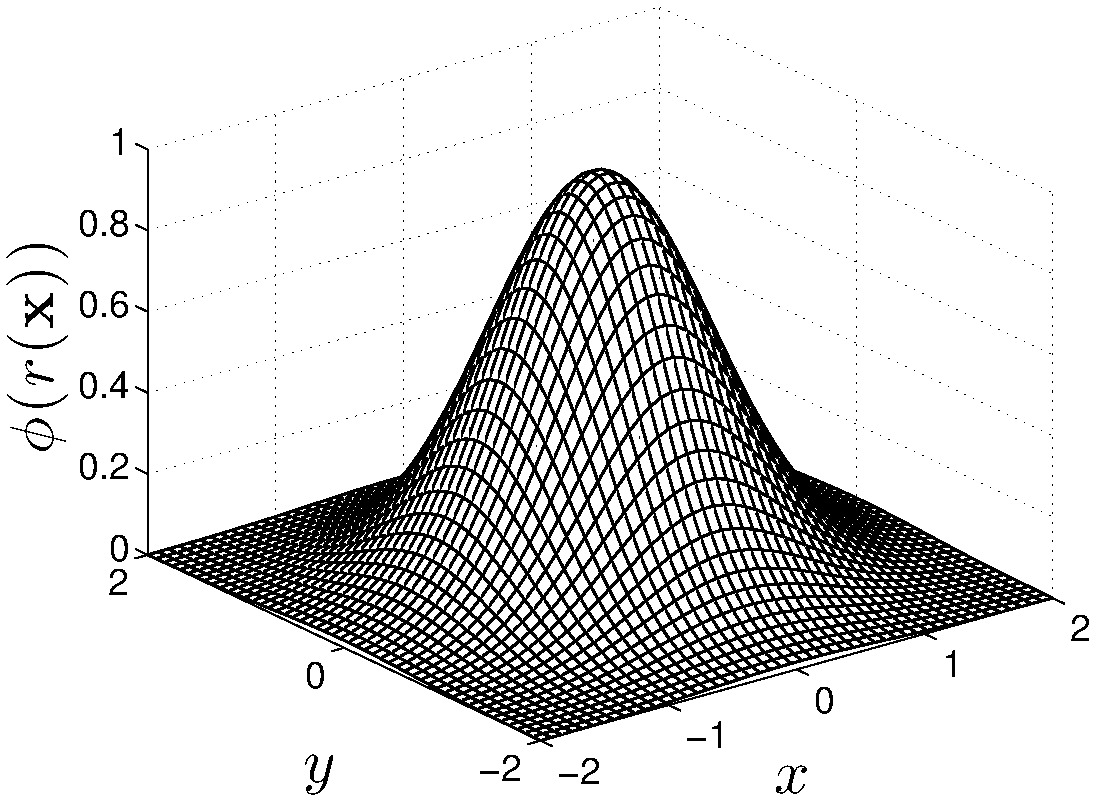
\includegraphics[width=1.0\textwidth]{../figures/paper1/figures/ga_rbf2d-eps-converted-to.pdf} 
		\caption{Gaussian}
	\end{subfigure}
	\begin{subfigure}[b]{0.25\textwidth}
	\centering
		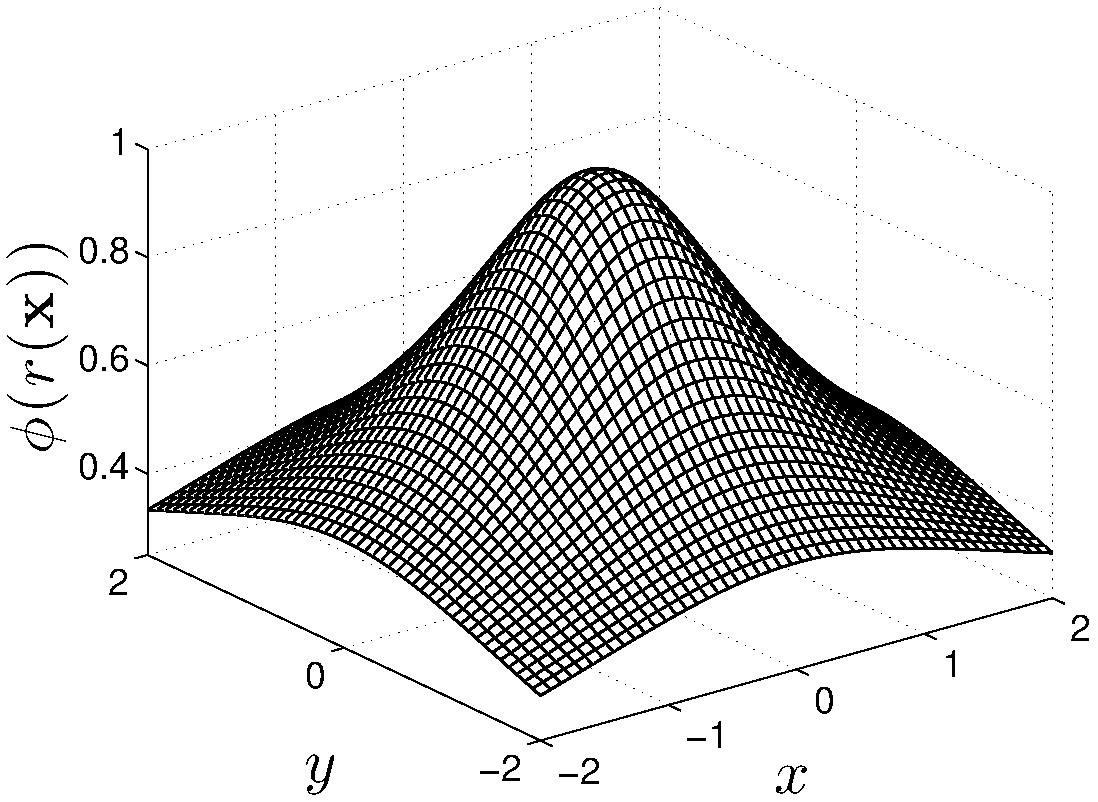
\includegraphics[width=1.0\textwidth]{../figures/paper1/figures/imq_rbf2d-eps-converted-to.pdf}
		\caption{Inverse Multiquadric}
	\end{subfigure}
	\begin{subfigure}[b]{0.25\textwidth}
	\centering
		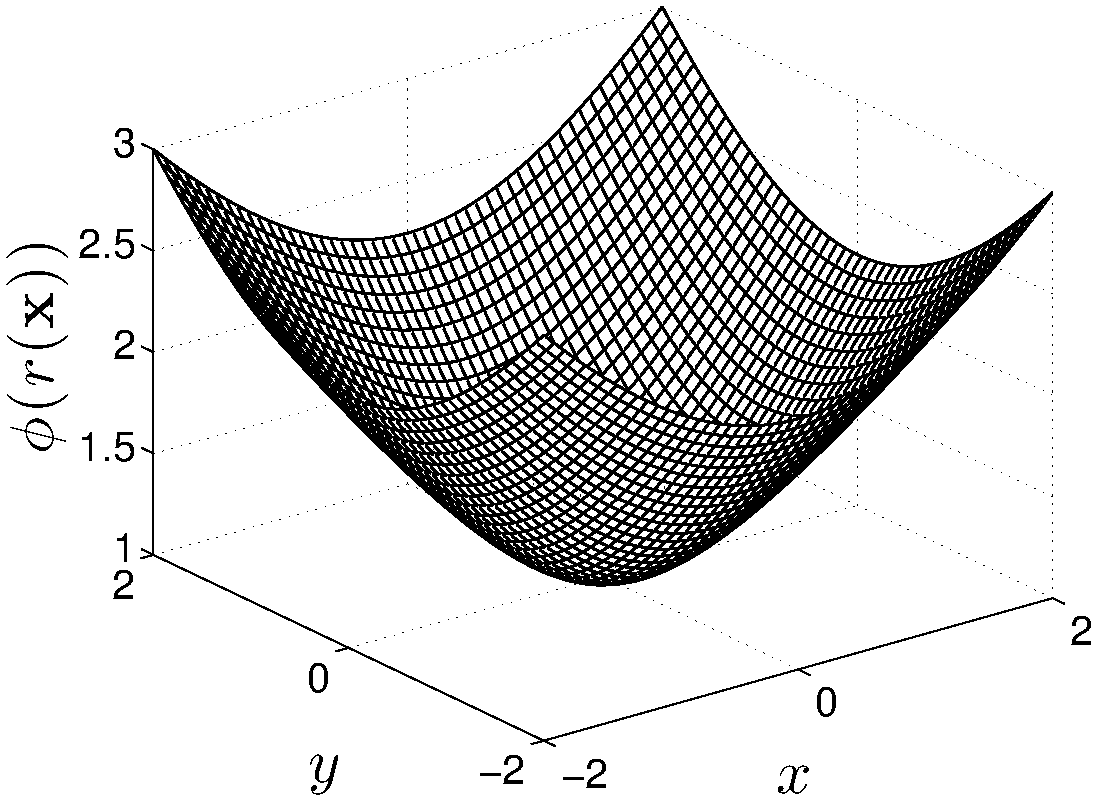
\includegraphics[width=1.0\textwidth]{../figures/paper1/figures/mq_rbf2d-eps-converted-to.pdf} 
		\caption{Multiquadric}
	\end{subfigure} 
    \caption{Commonly Used Radial Basis Functions (RBFs).}
    \label{fig:rbfs}
\end{figure}

At the core of all RBF-based PDE methods lies the fundamental problem of approximation/interpolation. Some methods (e.g., global- and compact-RBF methods) apply RBFs to approximate derivatives directly. Others (e.g., RBF-FD) leverage the basis functions to compute stencil weights, which in turn are used in generalized finite-difference approximations of derivatives. 

As ``meshless" methods, RBF methods excel at solving problems that require geometric flexibility with scattered node layouts in $d$-dimensional space. They naturally extend into higher dimensions with minimal increase in programming complexity \cite{FlyerWright07,WrightFlyerYuen10}. In addition to competitive accuracy and convergence compared with other state-of-the-art methods \cite{FlyerWright07, FlyerWright09, FlyerLehto10, WrightFlyerYuen10, FlyerFornberg11}, RBF methods boast stability for large time steps. Not all RBF methods are truly meshless. Most of them operate the same given an input set of nodes, whether or not the input includes an underlying mesh. However, some methods connect all nodes to all others (to be meshless), while methods like RBF-FD rely on stencils to connect points within small neighborhoods of one another. The generated stencils limit the scope of influence for nodes and complexity of the method, but also simulate a mesh. 

%Most literature surrounding RBF solutions for PDEs apply the concept of collocation (see Chapter~\ref{chap:background}). Recent trends in the community appear to have shifted, and RBF-FD seems to be top of the list. 


%RBF-FD is a hybrid of RBF scattered data interpolation and classical Finite Difference (FD). It shares many of the benefits from other RBF methods, like functionality on scattered node layouts in any dimension and high-order accurate solutions. Likewise, benefits akin to classical FD such as compact stencils for derivative approximation, and low computational complexity.

%Classical FD derivatives are expressed at a single node (center) as a weighted combination/difference of solution values from a small neighborhood (i.e., a stencil) around the center. Common approximations such as upwind differencing, center differencing, and other higher order approximations are of this form. 
%In similar fashion, RBF-FD combines solutions values based on stencils, but it does so in a more generalized sense than standard FD. For example, classical FD is typically restricted to regular meshes and often symmetric stencils in practice with the same set of weights for each stencil. Weights can be derived from polynomial expansion and obtained in 1D by solving a Vandermonde interpolation matrix \cite{FornbergLehto11}. Higher dimension FD stencils are composed from combinations of 1D formulas applied to each dimension. This implies restrictions on the shape/layout of stencils. In contrast to this, RBF-FD is designed for stencils with irregular node placement and can easily provide a unique set of weights for each stencil with no restrictions on stencil shape. 

%TODO:  \cite{Wright2004, Wright2003, WrightFornberg06, Chandhini2007}. 
To track the history of RBF methods, one must rewind to 1971 and R.L. Hardy's seminal research on interpolation with multi-quadric basis functions \cite{Hardy1971}. The transition from interpolation to RBF PDE methods dates back to 1990 \cite{Kansa1990a,Kansa1990b}. 
The RBF-FD method was first introduced in concept in 2000 \cite{Tolstykh2000}, but it took another few years for the method to really get a start (\cite{Shu2003}, \cite{Tolstykh2003a}, \cite{Wright2003} and \cite{Cecil2004}). Now a little over a decade old, the method is finally showing signs that it has the critical-mass following necessary for use in large-scale scientific models. At the onset of this work, most of the literature considered RBF-FD for problem sizes up to a few thousand nodes; at most into tens of thousands of nodes. Similar to most RBF methods, RBF-FD is predominantly implemented within small-scale, serial computing environments. The RBF community at-large continues to depend on MATLAB for investigation and extension development.

The goal of this dissertation is to scale RBF-FD solutions on high resolution meshes across high performance clusters, and to lead the way for its adoption within HPC and supercomputing circles. As part of this push to HPC, leveraging \emph{Graphics Processing Units (GPUs)} for computation is considered critical. GPUs, introduced in Chapter~\ref{chap:gpu_rbffd}, are many-core accelerators capable of general purpose, embarrassingly parallel computations. Accelerators represent the latest trend in HPC, where compute nodes are commonly supplemented by one or more accessory boards for offloading compute intensive tasks. Our effort leads the way for RBF-FD applicationss in an age when compute nodes with attached accelerator boards are considered key to breaching the exa-scale computing barrier \cite{GPUandExascale2011}. 

Parallelization of RBF-FD is achieved at two levels. On the first level, the
physical domain of the problem is partitioned
into overlapping subdomains, each handled by different MPI processes. All processes
operate independently to compute/load RBF-FD stencil weights, run diagnostic
tests and perform other initialization tasks. A process only computes weights
corresponding to stencils centered in the interior of its partition. After
initialization, processes work together to concurrently solve the PDE. Communication
barriers ensure that processes execute in lockstep and maintain consistent
solution values across the domain.  

The second level of
parallelization offloads tasks to the GPU at each iteration of the PDE solver. The bulk of computation in RBF-FD relies on a \emph{Sparse Matrix-Vector multiply (SpMV)} to evaluate derivatives. When mapped to the GPU, the SpMV operation is broken into two parts in order to overlap communication and computation, and amortize the cost of data transfer across multiple levels of hardware (see Chapter~\ref{chap:multigpu_rbffd}). 
% Although the stencil weight calculation is also data-parallel, we assume that in this context that the weights are precomputed and loaded once from disk during the initialization phase. 

%Additional key challenges lie in the choice of grid, the choice of stencil, and stability of scalable solutions. 
%To demonstrate Chapter~\ref{chap:applied_rbffd} verifies 


%
%Even today, RBFs are still up-and-coming in the scientific world with many avenues of research left to consider. Global formulations are understood to have spectral convergence properties, high accuracy and other benefits like adaptivity and ease of implementation over meshed methods \cite{Fasshauer:2007}. However, little is known about the behavior of local and RBF-FD methods. Open questions include (but are in no way limited to): a) ideal node placement to eliminate singularities; b) data-structures for stencil storage and evaluation; c) problem sizes larger than a few thousand nodes; and d) parallel implementations across new heterogeneous multi- and many-core architectures. In response to this, our group, in collaboration with researchers assembled from a national lab and four universities (see Chapter~\ref{chap:funding}), has been granted funds by the National Science Foundation to collaboratively:
%
%\begin{quote}
%\emph{``Bring RBFs to the forefront of multi-scale geophysical modeling by developing fast, efficient, and parallelizable RBF algorithms in arbitrary geometries, with performance enhanced by hardware accelerators, such as graphic processing units (GPUs)."} \cite{RBF_proposal:2009}
%\end{quote}
%
%



The layout of this document is as follows. This chapter continues with a survey of work related to parallelizing RBF-FD, targeting the GPU, and spanning a multi-GPU cluster. Chapter~\ref{chap:background} provides a historical survey of RBF methods as a backdrop to present RBF-FD in Chapter~\ref{chap:rbffd_method}. Chapter~\ref{chap:stencils} introduces a new algorithm for generating RBF-FD stencils as a faster alternative to the RBF community favorite, $k$-D Tree. In Chapter~\ref{chap:distributed_rbffd}, the first scalable implementation of RBF-FD to span one thousand processors is described in detail. Chapter~\ref{chap:gpu_rbffd} continues with the challenge of offloading computation to GPUs, and Chapter~\ref{chap:multigpu_rbffd} expands the discussion to RBF-FD on a multi-GPU cluster. In Chapter~\ref{chap:applications} the parallel RBF-FD implementation is applied and verified on the solutions of both explicit and implicit geophysical PDEs. Finally, Chapter~\ref{chap:conclusions} concludes with a summary of novel contributions, results and a discussion on future directions.

\section{On Parallel/Distributed RBF-FD} 

%TODO: why implement independent of PETSc, Deal.II, Trilinos, etc. 

%\authnote{Related work for start of Parallel/GPU chapter}
Parallel implementations of RBF methods rely on \emph{domain decomposition}. Depending on the implementation, domain decomposition not only accelerates solution procedures, but can decrease the ill-conditioning that plague all global RBF methods (\cite{Divo2007}). The ill-conditioning is reduced if each domain is treated as a separate RBF domain, and the boundary update is treated separately. Domain decomposition methods for RBFs were introduced by Beatson et al. \cite{Beatson2000}. Their work provided a solution to solve problem sizes into the millions of nodes.

This work leverages a domain decomposition, but not for the purpose of conditioning. Instead subdomains are distributed across multiple compute nodes and scaling RBF-FD across more than a thousand CPU cores of an HPC cluster. Add to this a twist to incorporate a novel implementation on the GPU with overlapping communication and computation. This combination is unmatched in related work. However, RBF methods do have a bit of history of parallel implementations. 

In 2007, Divo and Kassab \cite{Divo2007} used a domain decomposition method with artificial 
subdomain boundaries for their implementation of a local collocation method \cite{Divo2007}. 
The subdomains are processed independently, with derivative values 
at artificial boundary points averaged to maintain global consistency of physical values. Their implementation 
was designed for a 36 node cluster, but benchmarks and scalability tests are not provided.

% Divo: it seems almost unnecessary to use domain decomposition if they have the local method.
% I suppose the domain decomposition is necessary for averaging physical values more than RBF collocation.
However, research on the parallelization of RBF algorithms to solve PDEs on multiple CPU/GPU architectures is essentially non-existent. We have found three studies that have addressed this topic, none of which implement RBF-FD but rather take the avenue of domain decomposition for global RBFs (similar to a spectral element approach). In \cite{Divo2007}, Divo and Kassab introduce subdomains with artificial boundaries that are processed independently. Their implementation was designed for a 36 node cluster, but benchmarks and scalability tests are not provided. Kosec and \v{S}arler \cite{Kosec2008} parallelize coupled heat transfer and fluid flow models using OpenMP on a single workstation with one dual-core processor. They achieved a speedup factor of 1.85x over serial execution, although there were
no results from scaling tests. Yokota, Barba and Knepley \cite{Yokota2010} apply a restrictive additive Schwarz domain decomposition to parallelize global RBF interpolation of more then 50 million nodes on 1024 CPU processors.

Kosec and \v{S}arler \cite{Kosec2008} have the only known (to our knowledge) OpenMP implementation for RBFs. The authors parallelize coupled heat transfer 
and fluid flow problems on a single workstation. 
The application involves the local RBF collocation method, explicit time-stepping and Neumann boundary conditions. A speedup 
factor of 1.85x over serial execution was achieved by executing on two CPU cores; no further 
results from scaling tests were provided. 

Stevens et al. \cite{Stevens2009a} mention a parallel implementation under development, but no document is available at this time. 

Perhaps the most competitive parallel implementation of RBFs is the PetRBF branch of PETSc \cite{Yokota2010}. The authors of PetRBF have implemented a highly scalable, efficient RBF interpolation method based on compact RBFs (i.e., they operate on sparse matrices). The authors demonstrate efficient weak scaling of PetRBF across 1024 processes on a Blue Gene/L, and strong scaling up to 128 processes on the same hardware. On the Blue Gene/L, PetRBF is demonstrated to achieve an impressive 74\% parallel weak scaling efficiency on 1024 processes (operating on over 50 million points), and 84\% strong scaling efficiency for 128 processes. Strong scaling was also tested on a Cray XT4, where strong scaling tops out at 36\% for 128 processes, a respectable number---and similar to observed results for our own code on for the same number of processes (see Chapter~\ref{chap:distributed_rbffd}).  


%Within the scope of this paper we detail our method for spanning RBF-FD across multiple CPU/GPU processors and emphasize numerical validation of the implementation rather than optimization strategies. We will consider optimization in future work. The calculations are performed on Keeneland, a high performance computing installation supported by the National Science Foundation and located at Oak Ridge National Lab. Keeneland currently has 240 CPUs accompanied by 360 NVidia Fermi class GPUs with at least double that number expected by the end of 2012 \cite{Vetter2011}.



\section{On GPU RBF Methods (Incomplete)}

With regard to the latter, there is some research on leveraging RBFs on GPUs in the fields of visualization \cite{Cuntz2007,Weiler2005},  surface reconstruction \cite{Corrigan2005,Carr2003}, and neural networks \cite{Brandstetter2008}.

 %Originally GPUs were designed as parallel rasterizing units. They had limited logic control in contrast to the serial CPUs and their advanced branching and looping logic. 
%
%Gradually new and complex logic was added to the GPU to produce the shader languages that allowed developers to customize specific parts of the rendering pipeline. This allowed scientific problems such as the diffusion equation to be solved in process of rendering \cite{Harris2005}. In other words, the GPU was tricked into computing.
%
%The year 2006 brought the modern age of GPU computing with the introduction of CUDA from NVidia. The high level language allowed scientists to leverage the GPU as a parallel accelerator without all of the overhead of setting up graphics contexts and tricking the hardware into computing. Memory management is still the developer's responsibility, but compiler transforms generic C/Fortran code to GPU instruction set. 
%
%Scientific Computing has seen a widespread adoption of GPGPU because of the goal to get to ``exa-scale'' computing, which may only be possible in the near future with the help of GPU accelerators \cite{GPUandExascale2011}. 
%
%NVidia is not the only company involved in many core parallel accelerators. Other groups like AMD and Intel have been increasing the number of cores as well. The end effect is a hybridization where CPUs look similar to GPUs and vice-versa. 
%
%Until 2009, the hardware distinction required that developers target parallelism on CPUs and GPUs using different languages. Then the OpenCL standard was drafted and implemented. OpenCL is a parallel language that strives to provide functional portability rather than performance. 
%
%We focus on the OpenCL language within this dissertation with confidence that hardware will change frequently. In fact, every 18 months \cite{CudaGuide2011} shows a new release of GPU hardware, many-core CPU hardware and extensions to parallel languages. But if hardware is constantly changing, then one must focus on a high level implementation that allows portability across hardware. Enter the Open Compute Language (OpenCL) in 2009. OpenCL is standards based a to carry our implementations into the future regardless of what hardware and which company survive. 


Related work on RBFs and GPUs is sparse. In 2009, Schmidt et al. \cite{Schmidt2009a, Schmidt2009b} implemented a global RBF method for Tsunami simulation on the GPU using the AccelerEyes Jacket \cite{JacketGuide2009} add-on for MATLAB. Jacket provides a MATLAB interface to data structures and routines that internally call to the NVidia CUDA API. Their model was based on a single large dense matrix solve, and with the help of Jacket the authors were able to achieve approximately 7x speedup over the standard MATLAB solution on the then current generation of the MacBook Pro laptop. The authors compared the laptop CPU (processor details not specified) to the built-in NVidia GeForce 8600M GT GPU. Schmidt et al.'s implementation was the first contribution to the RBF community to leverage accelerators. The results were significant and promising, but no further contributions were made on the topic. 

While both Schmidt et al.'s method and the method presented here are based on RBFs, the two problems are only distantly related when it comes to implementation on the GPU. Dense matrix operations have a high computational complexity, are considered ideal (or near to) by linear algebra libraries like BLAS \cite{BLAS} and LAPACK \cite{Lapack1999}, and were demonstrated to fit well on GPUs from the onset of General Purpose GPU (GPGPU) Computing. In fact, NVidia included CUBLAS \cite{CudaToolkitDoc} (a GPU based BLAS library for their hardware) with their initial public release of the game-changing CUDA development kit in 2006. In stark contrast to this, sparse matrix operations have minimal computational complexity and are less than ideal for the GPU.


Earlier this year (2013), Cuomo et al. \cite{Cuomo2013} implemented RBF-interpolation on the GPU for surface reconstruction. Their implementation utilizes PetRBF \cite{Yokota2010}, and new built-in extensions that allow GPU access within PETSc. PETSc internally wraps the CUSP project \cite{Cusp2012} for sparse matrix algebra on the GPU. With the help of these libraries, Cuomo et al. solve and apply sparse interpolation systems on the GPU for up to three million nodes on an NVidia Fermi C1060 GPU (4GB). They compare results to a single core CPU implementation on an Intel i7-940 CPU and demonstrate that the GPU accelerate their solutions between 6x and 25x. Unfortunately, the authors do not show evidence of scaling the interpolation across multiple GPUs; so while evidence exists that PetRBF now has full GPU support, it remains to be seen how well the code can scale in GPU mode. 
 
\section{On Multi-GPU Methods}
 
Multi-GPU Jacobi iteration for Navier stokes flow in cavity \url{http://scholarworks.boisestate.edu/cgi/viewcontent.cgi?article=1003&context=mecheng_facpubs}

Thibault et al. have multiple works on Multi-GPU and overlapping comm and comp. 

The latest version of PETSc includes GPU support. PETSc is a widely-used library for distributed sparse and dense matrix algebra. 

\section{Major Contributions}

Within this thesis readers should expect to find the following major contributions to the communities surrounding RBF methods, GPGPU, and HPC: 
\begin{itemize} 
\item The first implementation of RBF-FD on GPUs, with one and many GPU environments considered. 
\begin{itemize} 
\item Multiple GPU kernels are tested, including custom OpenCL kernels for RK4 time-stepping and 
\end{itemize} 
\item The first implementation of RBF-FD on multiple CPUs through the use of domain decomposition
\item The first application of the Fixed-Grid neighbor query algorithm to generate stencils for RBF-FD. 
\end{itemize}



\ifstandalone
%Bei direkter Übersetzung sollte gleich noch das Literaturverzeichnis rein.
\bibliographystyle{plain}
\bibliography{merged_references}
\end{document}
\else
\expandafter\endinput
\fi


\makeatletter
\@ifundefined{standalonetrue}{\newif\ifstandalone}{}
\@ifundefined{section}{\standalonetrue}{\standalonefalse}
\makeatother
\ifstandalone
\documentclass[11pt]{report}

\usepackage{textcase}
%\usepackage{hyperref}
%\hypersetup{breaklinks=true}


% Added packages
\usepackage[usenames]{color}
\usepackage{amsfonts, amsmath, amssymb, graphics}

% NOTE: bibentry MUST appear before the hyperref or build will fail
\usepackage{bibentry}
\nobibliography*
\usepackage[square,sort,comma,numbers]{natbib}
  
\usepackage{float}
\usepackage[
	hidelinks,%
    %hyperindex=true,		% Make numbers of index links as well
   	backref=page, 		% Provide page listing where refs occur in the bibliography
	%breaklinks=true,
    %colorlinks,%
    %citecolor=green,%
    %filecolor=blue,%
    %linkcolor=red,%
    %urlcolor=red, 
]{hyperref}

\usepackage{dsfont}
%%%% USEPACKAGES for MACROS %%%%%
\usepackage{algpseudocode}
\usepackage[chapter]{algorithm}
%\usepackage{caption}
\usepackage{subcaption}
\usepackage{url}

\usepackage{array}
\usepackage{arydshln}
\usepackage{multirow}
\usepackage{multicol}
%\usepackage[section]{placeins}

\usepackage[usenames,dvipsnames]{color}
%\usepackage[english]{babel}
\usepackage{tabularx}
\usepackage{soul}
\usepackage{xparse}
\usepackage{listings}
%\usepackage[normalem]{ulem}



%%%%%%%%%%%%%%%
% Show a list of items "todo" or "done" 
% USAGE: 
% \begin{todolist} 
% 	\todo Something not finished
% 	\done Something finished
% \end{todolist} 
\newenvironment{todolist}{%
  \begin{list}{}{}% whatever you want the list to be
  \let\olditem\item
  \renewcommand\item{\olditem \textcolor{red}{(TODO)}: }
  \newcommand\todo{\olditem \textcolor{red}{(TODO)}: }
   \newcommand\done{\olditem \textcolor{ForestGreen}{(DONE)}: }
}{%
  \end{list}
} 
%%%%%%%%%%%%%%%

%%%%%%%%%%%%%%%
% Show a Author's Note
% USAGE: 
% \incomplete[Optional footnote message to further clarify note]{The text which is currently not finished}
\DeclareDocumentCommand \incomplete{ o m }
{%
\IfNoValueTF {#1}
{\textcolor{red}{Incomplete: \ul{#2}}} 
{\textcolor{red}{Incomplete: \ul{#2}}\footnote{Comment: #1}}%
}
%%%%%%%%%%%%%%%



%%%%%%%%%%%%%%%
% Show a Author's Note
% USAGE: 
% \authnote[Optional footnote message to further clarify note]{The note to your readers}
\DeclareDocumentCommand \authnote { o m }
{%
\IfNoValueTF {#1}
{\textcolor{blue}{Author's Note: \ul{#2}}} 
{\textcolor{blue}{Author's Note: \ul{#2}}\footnote{Comment: #1}}%
}
%%%%%%%%%%%%%%%



%%%%%%%%%%%%%%%
% Strike out text that doesn't belong in the paper
% USAGE: 
% \strike[Optional footnote to state why it doesn't belong]{Text to strike out}
\DeclareDocumentCommand \strike { o m }
{%
\setstcolor{Red}
\IfNoValueTF {#1}
{\textcolor{Gray}{\st{#2}}} 
{\textcolor{Gray}{\st{#2}}\footnote{Comment: #1}}%
}
%%%%%%%%%%%%%%%

\definecolor{light-gray}{gray}{0.95}

\newcommand{\cbox}[3]{
\ \\
\fcolorbox{#1}{#2}{
\parbox{\textwidth}{
#3
}
}
}

% Setup an environment similar to verbatim but which will highlight any bash commands we have
\lstnewenvironment{unixcmds}[0]
{
%\lstset{language=bash,frame=shadowbox,rulesepcolor=\color{blue}}
\lstset{ %
language=sh,		% Language
basicstyle=\ttfamily,
backgroundcolor=\color{light-gray}, 
rulecolor=\color{blue},
%frame=tb, 
columns=fullflexible,
%framexrightmargin=-.2\textwidth,
linewidth=0.8\textwidth,
breaklines=true,
%prebreak=/, 
  prebreak = \raisebox{0ex}[0ex][0ex]{\ensuremath{\hookleftarrow}},
%basicstyle=\footnotesize,       % the size of the fonts that are used for the code
%numbers=left,                   % where to put the line-numbers
%numberstyle=\footnotesize,      % the size of the fonts that are used for the line-numbers
%stepnumber=2,                   % the step between two line-numbers. If it's 1 each line 
                                % will be numbered
%numbersep=5pt,                  % how far the line-numbers are from the code
showspaces=false,               % show spaces adding particular underscores
showstringspaces=false,         % underline spaces within strings
showtabs=false,                 % show tabs within strings adding particular underscores
frame=single,	                % adds a frame around the code
tabsize=2,	                % sets default tabsize to 2 spaces
captionpos=b,                   % sets the caption-position to bottom
breakatwhitespace=false,        % sets if automatic breaks should only happen at whitespace
}
} { }

% Setup an environment similar to verbatim but which will highlight any bash commands we have
\lstnewenvironment{cppcode}[1]
{
%\lstset{language=bash,frame=shadowbox,rulesepcolor=\color{blue}}
\lstset{ %
	backgroundcolor=\color{light-gray}, 
	rulecolor=\color[rgb]{0.133,0.545,0.133},
	tabsize=4,
	language=[GNU]C++,
%	basicstyle=\ttfamily,
        basicstyle=\scriptsize,
        upquote=true,
        aboveskip={1.5\baselineskip},
        columns=fullflexible,
        %framexrightmargin=-.1\textwidth,
       %framexleftmargin=6mm,
        showstringspaces=false,
        extendedchars=true,
        breaklines=true,
        prebreak = \raisebox{0ex}[0ex][0ex]{\ensuremath{\hookleftarrow}},
        frame=single,
        showtabs=false,
        showspaces=false,
        showstringspaces=false,
        numbers=left,                   % where to put the line-numbers
	numberstyle=\footnotesize,      % the size of the fonts that are used for the line-numbers
	stepnumber=4,                   % the step between two line-numbers. If it's 1 each line 
                                % will be numbered
	firstnumber=#1,
         numbersep=5pt,                  % how far the line-numbers are from the code
        identifierstyle=\ttfamily,
        keywordstyle=\color[rgb]{0,0,1},
        commentstyle=\color[rgb]{0.133,0.545,0.133},
        stringstyle=\color[rgb]{0.627,0.126,0.941},
}
} { }

% Setup an environment similar to verbatim but which will highlight any bash commands we have
\lstnewenvironment{mcode}[1]
{
\lstset{ %
	backgroundcolor=\color{light-gray}, 
	rulecolor=\color[rgb]{0.133,0.545,0.133},
	tabsize=4,
	language=Matlab,
%	basicstyle=\ttfamily,
        basicstyle=\scriptsize,
        upquote=true,
        aboveskip={1.5\baselineskip},
        columns=fullflexible,
        %framexrightmargin=-.1\textwidth,
       %framexleftmargin=6mm,
        showstringspaces=false,
        extendedchars=true,
        breaklines=true,
        prebreak = \raisebox{0ex}[0ex][0ex]{\ensuremath{\hookleftarrow}},
        frame=single,
        showtabs=false,
        showspaces=false,
        showstringspaces=false,
        numbers=left,                   % where to put the line-numbers
	numberstyle=\footnotesize,      % the size of the fonts that are used for the line-numbers
	stepnumber=4,                   % the step between two line-numbers. If it's 1 each line 
                                % will be numbered
	firstnumber=#1,
         numbersep=5pt,                  % how far the line-numbers are from the code
        identifierstyle=\ttfamily,
        keywordstyle=\color[rgb]{0,0,1},
        commentstyle=\color[rgb]{0.133,0.545,0.133},
        stringstyle=\color[rgb]{0.627,0.126,0.941},
}
} { }

\newcommand{\inputmcode}[1]{%
\lstset{ %
	backgroundcolor=\color{light-gray},  %
	rulecolor=\color[rgb]{0.133,0.545,0.133}, %
	tabsize=4, %
	language=Matlab, %
%	basicstyle=\ttfamily,
        basicstyle=\scriptsize, %
        %        upquote=true,
        aboveskip={1.5\baselineskip}, %
        columns=fullflexible, %
        %framexrightmargin=-.1\textwidth,
       %framexleftmargin=6mm,
        showstringspaces=false, %
        extendedchars=true, %
        breaklines=true, %
        prebreak = \raisebox{0ex}[0ex][0ex]{\ensuremath{\hookleftarrow}}, %
        frame=single, %
        showtabs=false, %
        showspaces=false, %
        showstringspaces=false,%
        numbers=left,                   % where to put the line-numbers
	numberstyle=\footnotesize,      % the size of the fonts that are used for the line-numbers
	stepnumber=4,                   % the step between two line-numbers. If it's 1 each line 
                                % will be numbered
         numbersep=5pt,                  % how far the line-numbers are from the code
        identifierstyle=\ttfamily, %
        keywordstyle=\color[rgb]{0,0,1}, %
        commentstyle=\color[rgb]{0.133,0.545,0.133}, %
        stringstyle=\color[rgb]{0.627,0.126,0.941} %
}
\lstinputlisting{#1}%
}

%\lstset{ %
%	backgroundcolor=\color{light-gray}, 
%	rulecolor=\color[rgb]{0.133,0.545,0.133},
%	tabsize=4,
%	language=Matlab,
%%	basicstyle=\ttfamily,
%        basicstyle=\scriptsize,
%        upquote=true,
%        aboveskip={1.5\baselineskip},
%        columns=fullflexible,
%        %framexrightmargin=-.1\textwidth,
%       %framexleftmargin=6mm,
%        showstringspaces=false,
%        extendedchars=true,
%        breaklines=true,
%        prebreak = \raisebox{0ex}[0ex][0ex]{\ensuremath{\hookleftarrow}},
%        frame=single,
%        showtabs=false,
%        showspaces=false,
%        showstringspaces=false,
%        numbers=left,                   % where to put the line-numbers
%	numberstyle=\footnotesize,      % the size of the fonts that are used for the line-numbers
%	stepnumber=4,                   % the step between two line-numbers. If it's 1 each line 
%                                % will be numbered
%	firstnumber=#1,
%         numbersep=5pt,                  % how far the line-numbers are from the code
%        identifierstyle=\ttfamily,
%        keywordstyle=\color[rgb]{0,0,1},
%        commentstyle=\color[rgb]{0.133,0.545,0.133},
%        stringstyle=\color[rgb]{0.627,0.126,0.941},
%}


\newcommand{\Laplacian}[1]{\nabla^2 #1}

% set of all nodes received and contained on GPU
\newcommand{\setAllNodes}[0]{\mathcal{G}}
% set of stencil centers on GPU
\newcommand{\setCenters}[0]{\mathcal{Q}}
% set of stencil centers with nodes in \setDepend
\newcommand{\setBoundary}[0]{\mathcal{B}}
% set of nodes received by other GPUs
\newcommand{\setDepend}[0]{\mathcal{R}}
% set of nodes sent to other GPUs
\newcommand{\setProvide}[0]{\mathcal{O}}


\newcommand{\toprule}[0]{\hline}
\newcommand{\midrule}[0]{\hline\hline}
\newcommand{\bottomrule}[0]{\hline}

\newcolumntype{C}{>{\centering\arraybackslash}b{1in}}
\newcolumntype{L}{>{\flushleft\arraybackslash}b{1.5in}}
\newcolumntype{R}{>{\flushright\arraybackslash}b{1.5in}}
\newcolumntype{D}{>{\flushright\arraybackslash}b{2.0in}}
\newcolumntype{E}{>{\flushright\arraybackslash}b{1.0in}}

\DeclareSymbolFont{AMSb}{U}{msb}{m}{n}
\DeclareMathSymbol{\N}{\mathbin}{AMSb}{"4E}
\DeclareMathSymbol{\Z}{\mathbin}{AMSb}{"5A}
\DeclareMathSymbol{\R}{\mathbin}{AMSb}{"52}
\DeclareMathSymbol{\Q}{\mathbin}{AMSb}{"51}
\DeclareMathSymbol{\PP}{\mathbin}{AMSb}{"50}
\DeclareMathSymbol{\I}{\mathbin}{AMSb}{"49}
%\DeclareMathSymbol{\C}{\mathbin}{AMSb}{"43}

%%%%%% VECTOR NORM: %%%%%%%
\newcommand{\vectornorm}[1]{\left|\left|#1\right|\right|}
\newcommand{\vnorm}[1]{\left|\left|#1\right|\right|}
\newcommand{\by}[0]{\times}
\newcommand{\vect}[1]{\mathbf{#1}}
%\newcommand{\mat}[1]{\mathbf{#1}} 

%\renewcommand{\vec}[1]{ \textbf{#1} }
%%%%%%%%%%%%%%%%%%%%%%

%%%%%%% THM, COR, DEF %%%%%%%
%\newtheorem{theorem}{Theorem}[section]
%\newtheorem{lemma}[theorem]{Lemma}
%\newtheorem{proposition}[theorem]{Proposition}
%\newtheorem{corollary}[theorem]{Corollary}
%\newenvironment{proof}[1][Proof]{\begin{trivlist}
%\item[\hskip \labelsep {\bfseries #1}]}{\end{trivlist}}
%\newenvironment{definition}[1][Definition]{\begin{trivlist}
%\item[\hskip \labelsep {\bfseries #1}]}{\end{trivlist}}
%\newenvironment{example}[1][Example]{\begin{trivlist}
%\item[\hskip \labelsep {\bfseries #1}]}{\end{trivlist}}
%\newenvironment{remark}[1][Remark]{\begin{trivlist}
%\item[\hskip \labelsep {\bfseries #1}]}{\end{trivlist}}
%\newcommand{\qed}{\nobreak \ifvmode \relax \else
%      \ifdim\lastskip<1.5em \hskip-\lastskip
%      \hskip1.5em plus0em minus0.5em \fi \nobreak
%      \vrule height0.75em width0.5em depth0.25em\fi}
%%%%%%%%%%%%%%%%%%%%%%

%
%\usepackage[algochapter]{algorithm2e}
%\usepackage[usenames]{color}
% colors to show the corrections
\newcommand{\red}[1]{\textbf{\textcolor{red}{#1}}}
\newcommand{\blue}[1]{\textbf{\textcolor{blue}{#1}}}
\newcommand{\cyan}[1]{\textbf{\textcolor{cyan}{#1}}}
\newcommand{\green}[1]{\textbf{\textcolor{green}{#1}}}
\newcommand{\magenta}[1]{\textbf{\textcolor{magenta}{#1}}}
\newcommand{\orange}[1]{\textbf{\textcolor{orange}{#1}}}
%%%%%%%%%% DK DK
% comments between authors
\newcommand{\toall}[1]{\textbf{\green{@@@ All: #1 @@@}}}
\newcommand{\toevan}[1]{\textbf{\red{*** Evan: #1 ***}}}
%\newcommand{\toevan}[1]{}  % USE FOR FINAL VERSION
\newcommand{\toe}[1]{\textbf{\red{*** Evan: #1 ***}}}
\newcommand{\tog}[1]{\textbf{\blue{*** Gordon: #1 ***}}}
%\newcommand{\togordon}[1]{\textbf{\blue{*** Gordon: #1 ***}}}
\renewcommand{\ge}[3]{{\textcolor{blue}{*** \textbf{Gordon:}\strike{#1} #2 ***}}\red{(#3)}}
\renewcommand{\ge}[3]{{\textcolor{blue}{#2}}}
\renewcommand{\ge}[3]{{\textcolor{Red}{#2}}}
\newcommand{\eb}[3]{{\textcolor{Red}{*** \textbf{Evan:}\strike{#1} #2 ***}}\red{(#3)}}
\renewcommand{\eb}[3]{{{\textcolor{Red}{#2}}}}
%\def\ge#1#2#3{}{\textbf{\blue{*** Gordon: #2 ***}}}{(#3)}
\newcommand{\gee}[1]{{\bf{\blue{{\em #1}}}}}
\newcommand{\old}[1]{}
\newcommand{\del}[1]{***#1*** }



% \DeclareMathOperator{\Sample}{Sample}
%\let\vaccent=\v % rename builtin command \v{} to \vaccent{}
%\renewcommand{\vec}[1]{\ensuremath{\mathbf{#1}}} % for vectors
\newcommand{\gv}[1]{\ensuremath{\mbox{\boldmath$ #1 $}}} 
% for vectors of Greek letters
\newcommand{\uv}[1]{\ensuremath{\mathbf{\hat{#1}}}} % for unit vector
\newcommand{\abs}[1]{\left| #1 \right|} % for absolute value
\newcommand{\avg}[1]{\left< #1 \right>} % for average
\let\underdot=\d % rename builtin command \d{} to \underdot{}
\renewcommand{\d}[2]{\frac{d #1}{d #2}} % for derivatives
\newcommand{\dd}[2]{\frac{d^2 #1}{d #2^2}} % for double derivatives
\newcommand{\pd}[2]{\frac{\partial #1}{\partial #2}} 
% for partial derivatives
\newcommand{\pdd}[2]{\frac{\partial^2 #1}{\partial #2^2}} 
\newcommand{\pdda}[3]{\frac{\partial^2 #1}{\partial #2 \partial #3}} 
% for double partial derivatives
\newcommand{\pdc}[3]{\left( \frac{\partial #1}{\partial #2}
 \right)_{#3}} % for thermodynamic partial derivatives
\newcommand{\ket}[1]{\left| #1 \right>} % for Dirac bras
\newcommand{\bra}[1]{\left< #1 \right|} % for Dirac kets
\newcommand{\braket}[2]{\left< #1 \vphantom{#2} \right|
 \left. #2 \vphantom{#1} \right>} % for Dirac brackets
\newcommand{\matrixel}[3]{\left< #1 \vphantom{#2#3} \right|
 #2 \left| #3 \vphantom{#1#2} \right>} % for Dirac matrix elements
\newcommand{\grad}[1]{\gv{\nabla} #1} % for gradient
\let\divsymb=\div % rename builtin command \div to \divsymb
\renewcommand{\div}[1]{\gv{\nabla} \cdot #1} % for divergence
\newcommand{\curl}[1]{\gv{\nabla} \times #1} % for curl
\let\baraccent=\= % rename builtin command \= to \baraccent
\renewcommand{\=}[1]{\stackrel{#1}{=}} % for putting numbers above =
\newcommand{\diffop}[1]{\mathcal{L}#1}
\newcommand{\boundop}[1]{\mathcal{B}#1}
\newcommand{\rvec}[0]{{\bf r}}

\newcommand{\Interior}[0]{\Omega}
\newcommand{\domain}[0]{\Omega}
%\newcommand{\Boundary}[0]{\partial \Omega}
\newcommand{\Boundary}[0]{\Gamma}

\newcommand{\on}[1]{\hskip1.5em \textrm{ on } #1}

\newcommand{\gemm}{\texttt{GEMM}}
\newcommand{\trmm}{\texttt{TRMM}}
\newcommand{\gesvd}{\texttt{GESVD}}
\newcommand{\geqrf}{\texttt{GEQRF}}


\newcommand{\minitab}[2][l]{\begin{tabular}{#1}#2\end{tabular}}
\newcommand{\comm}[1]{\textcolor{red}{\textit{#1}}}

\newcommand{\nfrac}[2]{
\nicefrac{#1}{#2}
%\frac{#1}{#2}
}

\usepackage{xparse}
\usepackage{soul}


%%%%%%%%%%%%%%%
% Show a Author's Note
% USAGE: 
% \incomplete[Optional footnote message to further clarify note]{The text which is currently not finished}
\DeclareDocumentCommand \incomplete{ o m }
{%
\IfNoValueTF {#1}
{\textcolor{red}{Incomplete: \ul{#2}}} 
{\textcolor{red}{Incomplete: \ul{#2}}\footnote{Comment: #1}}%
}
%%%%%%%%%%%%%%%



%%%%%%%%%%%%%%%
% Show a Author's Note
% USAGE: 
% \authnote[Optional footnote message to further clarify note]{The note to your readers}
\DeclareDocumentCommand \authnote { o m }
{%
\IfNoValueTF {#1}
{\textcolor{blue}{Author's Note: \ul{#2}}} 
{\textcolor{blue}{Author's Note: \ul{#2}}\footnote{Comment: #1}}%
}
%%%%%%%%%%%%%%%



%%%%%%%%%%%%%%%
% Strike out text that doesn't belong in the paper
% USAGE: 
% \strike[Optional footnote to state why it doesn't belong]{Text to strike out}
\DeclareDocumentCommand \strike { o m }
{%
\setstcolor{red}
\IfNoValueTF {#1}
{\textcolor{Gray}{\st{#2}}} 
{\textcolor{Gray}{\st{#2}}\footnote{Comment: #1}}%
}
%%%%%%%%%%%%%%%



%
% colors to show the corrections
\newcommand{\red}[1]{\textbf{\textcolor{red}{#1}}}
\newcommand{\blue}[1]{\textbf{\textcolor{blue}{#1}}}
\newcommand{\cyan}[1]{\textbf{\textcolor{cyan}{#1}}}
\newcommand{\green}[1]{\textbf{\textcolor{green}{#1}}}
\newcommand{\magenta}[1]{\textbf{\textcolor{magenta}{#1}}}
\newcommand{\orange}[1]{\textbf{\textcolor{orange}{#1}}}
%%%%%%%%%% DK DK
% comments between authors
\newcommand{\toall}[1]{\textbf{\green{@@@ All: #1 @@@}}}
\newcommand{\toevan}[1]{\textbf{\red{*** Evan: #1 ***}}}
%\newcommand{\toevan}[1]{}  % USE FOR FINAL VERSION
\newcommand{\toe}[1]{\textbf{\red{*** Evan: #1 ***}}}
\newcommand{\tog}[1]{\textbf{\blue{*** Gordon: #1 ***}}}
%\newcommand{\togordon}[1]{\textbf{\blue{*** Gordon: #1 ***}}}
\renewcommand{\ge}[3]{{\textcolor{blue}{*** \textbf{Gordon:}\strike{#1} #2 ***}}\red{(#3)}}
\renewcommand{\ge}[3]{{\textcolor{blue}{#2}}}
\renewcommand{\ge}[3]{{\textcolor{red}{#2}}}
\newcommand{\eb}[3]{{\textcolor{red}{*** \textbf{Evan:}\strike{#1} #2 ***}}\red{(#3)}}
\renewcommand{\eb}[3]{{{\textcolor{red}{#2}}}}
%\def\ge#1#2#3{}{\textbf{\blue{*** Gordon: #2 ***}}}{(#3)}
\newcommand{\gee}[1]{{\bf{\blue{{\em #1}}}}}
\newcommand{\old}[1]{}
\newcommand{\del}[1]{***#1*** }



% Rename  this file          misc_mac.tex
%----------------------------------------------------------------------
%%%%%%%%%%%%%%%%%%%%%%%%%%%%%%%%%%%%%%%%%%%%%%%%%%%%%%%%%%%%%%%%%%%%%%%%%%%%%%%
%
%	Math Symbols   Math Symbols   Math Symbols   Math Symbols   
%
%%%%%%%%%%%%%%%%%%%%%%%%%%%%%%%%%%%%%%%%%%%%%%%%%%%%%%%%%%%%%%%%%%%%%%%%%%%%%%%
\def\pmb#1{\setbox0=\hbox{$#1$}%
	\kern-.025em\copy0\kern-\wd0
	\kern.05em\copy0\kern-\wd0
	\kern-.025em\raise.0433em\box0}
\def\pmbf#1{\pmb#1}
\def\bfg#1{\pmb#1}

% BETTER VALUES FOR AUTOMATIC FIGURE PLACEMENT THAN THOSE PROVIDED BY 
% LATEX DEFAULTS.

\renewcommand{\textfloatsep}{1ex}
\renewcommand{\floatpagefraction}{0.9}
\renewcommand{\intextsep}{1ex}
\renewcommand{\topfraction}{.9}
\renewcommand{\bottomfraction}{.9}
\renewcommand{\textfraction}{.1}

% #1  position of floating figure (h|t|b|p)
% #1  EPS postscript file
% #2  size
% #3  caption

%usage of newfig:
%  \newfig{file.ps}{3in}{Fig1: this is a figure}

\input{epsf}
\def\newfig#1#2#3{
  \begin{figure}[htbp]
  \vspace{1ex}
  \setlength{\epsfxsize}{#2}
  \centerline{\epsfbox{#1}}
  \vspace{-.1in}\caption{\small #3}\break\vspace{.2in}
  \label{#1}
  \end{figure}
}

%usage of newfigtwo: 2 figures, vertically stacked
% \newfig
%	{file1.ps}
%	{file2.ps}
%	{width}
%	{vertical space}
%	{Caption}

\def\newfigtwo#1#2#3#4#5{
  \begin{figure}[htbp]
  \vspace{1ex}
  \setlength{\epsfxsize}{#3}
  \centerline{\epsfbox{#1}}
  \vspace{#4}
  \setlength{\epsfxsize}{#3}
  \centerline{\epsfbox{#2}}
  \vspace{-.1in}\caption{\small #5}\break\vspace{.2in}
  \label{#1}
  \end{figure}
}

\def\newfigh#1#2#3#4{  % add height specification
  \begin{figure}[htbp]
  \vspace{1ex}
  \setlength{\epsfxsize}{#2}
  \setlength{\epsfysize}{#4}
  \centerline{\epsfbox{#1}}
  \vspace{-.1in}\caption{\small #3}\break\vspace{.2in}
  \label{#1}
  \end{figure}
}

\def\herefig#1#2#3{
  \begin{figure}[h]
  \setlength{\epsfxsize}{#2}
  \centerline{\epsfbox{#1}}
  \caption{\small #3}
  \label{#1}
  \end{figure}
}

\def\etal{{{\em et~al.\,\,}}}
\def\note#1{\\ =====#1===== \\}
\def\FBOX#1{\ \\ \fbox{\begin{minipage}{5in}#1\end{minipage}}\\ }
\newcount\sectionno     \sectionno=0
\newcount\eqnum         \eqnum=0
\def\addeqno{\global\advance \eqnum by  1 }
\def\subeqno{\global\advance \eqnum by -1 }
%\def\eqn{\addeqno \eqno \hbox{(\number\sectionno.\number\eqnum)} }

\def\tildetilde#1{\tilde{\tilde{#1}}}
\def\barbar#1{\overbar{\overbar{#1}}}

\def\vsp#1{\vspace{#1 ex}}
\def\fpar{\hspace{\parindent}}
%
%  \pf : 2 arguments: numerator and denominator of partial derivative
%
\def\pf#1#2{{\frac{\partial{#1}}{\partial{#2}}}}
\def\pfs#1#2{{\partial_{#2}{#1}}}
\def\pftwo#1#2{{\frac{\partial^2{#1}}{\partial{#2}^2}}}
\def\pfxx#1#2{{\frac{\partial^2{#1}}{\partial{#2}^2}}}
%\def\pfxy#1#2{{\frac{\partial^2{#1}}{\partial{#2}\partial{#3}}}}
\def\pfn#1#2#3{{\frac{\partial^{#1}{#2}}{\partial{#3}^{#1}}}}
\def\df#1#2{{\frac{d{#1}}{d{#2}}}}
\def\dfn#1#2#3{{\frac{d^{#1}{#2}}{d{#3}^{#1}}}}
\def\Dt#1#2{\frac{D#1}{D#2}}
\def\dt#1#2{\frac{d#1}{d#2}}
\def\bld#1{{\bf #1}}
\def\pfp#1#2#3{\pf{}{#3}{\left(\frac{#1}{#2}\right)}}

\def\norm#1{\|#1\|}

%
% Graphic characters  (\dot already defined by TeX/LateX)
%
\def\dash{\rule[1.5pt]{2mm}{.3mm}\HS{.9mm}}
\def\dott{\rule[1.5pt]{.7mm}{.3mm}\HS{.7mm}}
\def\dashline{\dash\dash\dash}
\def\dotline{\dott\dott\dott\dott\dott\dott}
\def\dashdotline{\dash$\cdot$\HS{.9mm}\dash}
\def\solidline{\rule[2pt]{7mm}{.3mm}}
% 
% overcircle
%
\def\ovcircle#1{\buildrel{\circ}\over{#1}}
%\def\below#1#2{\buildrel{#2}\under{#1}}
%\def\above#1#2{\buildrel{#2}\over{#1}}
%
%  big parenthesis and brackets
%
\def\bigpar#1#2{{\left(\frac{#1}{#2}\right)}}
\def\bigbra#1#2{{\left\[\frac{#1}{#2}\right\]}}

\def\Lp{\left(}
\def\Rp{\right)}
\def\Lb{\left[}
\def\Rb{\right]}
\def\Ln{\left\langle}
\def\Rn{\right\rangle}
\def\Ld{\left.}
\def\Rd{\right.}
\def\Lv{\left|}
\def\Rv{\right|}
\def\Lbr{\left|}
\def\Rbr{\right|}
\def\lng{\langle}
\def\rng{\rangle}
\def\Lc{\left\{}
\def\Rc{\right\}}
%%% %

% Cannot be handled by Lyx
%\def\[{{[}}
%\def\]{{]}}

%
\def\eol{\nonumber \\}
\def\eolnonb{\nonumber\\}
\def\eolnb{\\}
\def\nonb{\nonumber}
\def\be{\begin{equation}}
\def\ee{\end{equation}}
\def\BEQNA{\begin{eqnarray}}
\def\EEQNA{\end{eqnarray}}
\def\eqa{&=&}
\def\beqna{\begin{eqnarray}}
\def\eeqna{\end{eqnarray}}
\def\bverb{\begin{verbatim}}
\def\everb{\end{verbatim}}
\def\VERB#1{\bverb #1 \everb}
\def\btbl{\begin{tabular}}
\def\etbl{\end{tabular}}
\def\bmini{\begin{minipage}[t]{5.5in}}
\def\emini{\end{minipage}}
\def\parray#1#2{\left(\begin{array}{#1}#2\end{array}\right)}
\def\barray#1#2{\left[\begin{array}{#1}#2\end{array}\right]}
\def\carray#1#2{\left\{\begin{array}{#1}#2\end{array}\right.}
\def\darray#1#2{\left|\begin{array}{#1}#2\end{array}\right|}

\def\BEGTABLE#1{\begin{table}[hbt]\vspace{2ex}\begin{center}\bmini\centering\btbl{#1}}
\def\ENDTABLE#1#2{\etbl\caption[#1]{#2}\EMINI\end{center}\vspace{2ex}\end{table}}

\def\bfltbl#1{\begin{table}[hbt]\vspace{2ex}\begin{center}\bmini\centering\btbl{#1}}
\def\efltbl#1#2{\etbl\caption[#1]{#2}\emini\end{center}\vspace{2ex}\end{table}}
\def\mcol{\multicolumn}
%
%  label equations with (#)
%
\def\reff#1{(\ref{#1})}
%
%  macros borrowed from viewgraph package
%

\newenvironment{LETTRS}[3]{\begin{letter}{#1}
\input{origin}\opening{Dear #2:}\input{#3}\closing{Sincerely yours,}\end{letter}}{\clearpage}

\newenvironment{VIEW}[1]{{\BC\Huge\bf #1 \EC}\LARGE\VS{.05in}}{\clearpage}

\def\RM#1{\rm{#1\ }}
\def\BV{\begin{VIEW}}
\def\EV{\end{VIEW}}

\def\NI{\noindent}

\def\VS{\vspace*}
\def\HS{\hspace*}
\def\IT{\item}

\def\BARR{\begin{array}}
\def\EARR{\end{array}}

\def\BPARR{\left(\begin{array}}
\def\EPARR{\end{array}\right)}

\def\BDET{\left|\begin{array}}
\def\EDET{\end{array}\right|}

\def\BDF{\begin{definition}}
\def\EDF{\end{definition}}

\def\BSU{\begin{block}{Summary}}
\def\ESU{\end{block}}

\def\BEX{\begin{example}}
\def\EEX{\end{example}}

\def\BTH{\begin{theorem}}
\def\ETH{\end{theorem}}

\def\BCO{\begin{corollary}}
\def\ECO{\end{corollary}}

\def\BPROOF{\begin{proof}}
\def\EPROOF{\end{proof}}

\def\BLM{\begin{lemma}}
\def\ELM{\end{lemma}}

\def\BEQ{\begin{equation}}
\def\EEQ{\end{equation}}

\def\BEQNNB{$$}
\def\EEQNNB{$$}

\def\BE{\begin{enumerate}}
\def\EE{\end{enumerate}}

\def\BD{\begin{description}}
\def\ED{\end{description}}

\def\BI{\begin{itemize}}
\def\EI{\end{itemize}}

\def\BC{\begin{center}}
\def\EC{\end{center}}

\def\BFIG{\begin{figure}}
\def\EFIG{\end{figure}}

\def\BTABB{\begin{tabbing}}
\def\ETABB{\end{tabbing}}

\def\BMINI{\begin{minipage}}
\def\EMINI{\end{minipage}}

\def\BTABLE{\begin{table}}
\def\ETABLE{\end{table}}

\def\BTABUL{\begin{tabular}}
\def\ETABUL{\end{tabular}}

\def\MCOL{\multicolumn}
\def\UL{\underline}
\def\ULL#1{\UL{\UL{#1}}}

\def\BDOC{\begin{document}}
\def\EDOC{\end{document}}

\def\EM#1{{\em #1\/}}
\def\FN{\footnote}

% Courtesy of Ugo Piomelli

\def\latexfig #1 #2 #3 #4 #5 {\ \vfill
\hfill\hbox to 0.05in{\vbox to #3truein{
         \special{psfile="#1" angle=270 hscale=100 
                  hoffset=#4 voffset=#5 vscale=100} }\hfill}
\hfill\vspace{-0.1in}        }

% #1 is the .ps filename
% #2 is not used in the present version
% #3 is the size of the white space left above the caption (in inches)
% #4 is the horizontal offset from some unknown reference point.
%    It is in 1/72 of an inch and is positive to the right.
% #5 is the vertical offset from some unknown reference point.
%    It is in 1/72 of an inch and is positive upwards.


\newcommand{\mathsym}[1]{{}}
\newcommand{\unicode}[1]{{}}
\newcommand{\ep}{\epsilon}
\newcommand{\vv}{\mathbf{v}}
\newcommand{\vu}{\mathbf{u}}
\newcommand{\vx}{\mathbf{x}}

\newcommand{\Laplacian}[1]{\nabla^2 #1}
\newcommand{\LaplaceBeltrami}[1]{\Delta_S #1}

% set of all nodes received and contained on GPU
\newcommand{\setAllNodes}[0]{\mathcal{G}}
% set of stencil centers on GPU
\newcommand{\setCenters}[0]{\mathcal{Q}}
% set of stencil centers with nodes in \setDepend
\newcommand{\setBoundary}[0]{\mathcal{B}}
% set of nodes received by other GPUs
\newcommand{\setDepend}[0]{\mathcal{R}}
% set of nodes sent to other GPUs
\newcommand{\setProvide}[0]{\mathcal{O}}





\usepackage{tabularx} 
\newcolumntype{C}{>{\centering\arraybackslash}b{1in}}
\newcolumntype{L}{>{\flushleft\arraybackslash}b{1.5in}}
\newcolumntype{R}{>{\flushright\arraybackslash}b{1.5in}}
\newcolumntype{D}{>{\flushright\arraybackslash}b{2.0in}}
\newcolumntype{E}{>{\flushright\arraybackslash}b{1.0in}}


 


%\usepackage{xcolor}

%\usepackage{refcheck}
% Sepia
%\definecolor{myBGcolor}{HTML}{F6F0D6}
%\definecolor{myTextcolor}{HTML}{4F452C}
% Dark
%\definecolor{myBGcolor}{HTML}{3E3535}
%\definecolor{myTextcolor}{HTML}{CFECEC}
%\color{myTextcolor}
%\pagecolor{myBGcolor}
 
\usepackage[margin=1.25in]{geometry}
\usepackage{xcolor}

% Sepia
%\definecolor{myBGcolor}{HTML}{F6F0D6}
%\definecolor{myTextcolor}{HTML}{4F452C}

\definecolor{myBGcolor}{HTML}{3E3535}
\definecolor{myTextcolor}{HTML}{CFECEC}
%\pagecolor{myBGcolor}
%\color{myTextcolor}

\begin{document}
\tableofcontents
\fi

{ \graphicspath{{rbffd_methods_content/}} 

%introduction
%	- argue what we show within (i.e., first GPGPU, first multi-CPU, approximate nearest neighbors, etc.)
%numerical method
%	- TOD: Explain that preliminaries cover status entering the field
%		- DONE: global RBFs formulation, applications
%		- DONE: compact RBFs formulation, applications
%	- which brings us to our method of choice, RBF-FD
%		- Benefits in complexity, versatility
%		- inherits global RBFs
%		- new method with limited application
%implementation
%	- describe our neighbor queries
%		- approximate neighbors are good enough
%		- benchmark performance of kDTree vs LSH Raster
%		- Plot bandwidth of each method vs N on sphere
%		- 



\part{Preliminaries}


\chapter{RBF Methods for PDEs}

The process of solving partial differential equations (PDEs) using radial basis functions (RBFs) dates back to 1990 \cite{Kansa1990a,Kansa1990b}. However, at the core of all RBF methods lies the fundamental problem of approximation/interpolation. Some methods (e.g., global- and compact-RBF methods) apply RBFs to approximate derivatives directly. Others (e.g., RBF-generated Finite Differences) leverage the basis functions to generate weights for finite-differencing stencils, utilizing the weights in turn to approximate derivatives. Regardless, to track the history of RBF methods, one must look back to 1971 and R.L. Hardy's seminal research on interpolation with multi-quadric basis functions \cite{Hardy1971}. 

As ``meshless" methods, RBF methods excel at solving problems that require geometric flexibility with scattered node layouts in $d$-dimensional space. They naturally extend into higher dimensions without significant increase in programming complexity \cite{FlyerWright07,WrightFlyerYuen10}. In addition to competitive accuracy and convergence compared with other state-of-the-art methods \cite{FlyerWright07, FlyerWright09, FlyerLehto10, WrightFlyerYuen10, FlyerFornberg11}, they also boast stability for large time steps.

This chapter is dedicated to summarizing the four-decade history of RBF methods leading up to the development of the 
RBF-generated Finite Differences (RBF-FD) method. Beginning with a brief introduction to RBFs and a historical survey, we attempt to classify related work into three three types: global, compact, and local methods. Following this, the general approximation problem is introduced, with a look at the core of all three method classificiations: RBF scattered-data interpolation. %We categorize existing methods for solving PDEs with RBFs as either global 
%or local. Global methods use collocation and invert a single large linear system to find the interpolant that satisfies 
%the differential equations at RBF centers. Local methods limit the influence of basis functions and seek an interpolant 
%at each RBF center defined in terms of neighboring basis functions (local collocation) or nodal values (RBF-FD).

Three global RBF collocation methods are presented: Kansa's method, Fasshauer's method and Direct collocation. Within the historical context of RBF methods we highlight extensions that lead to local interpolation matrices instead of a single global interpolation matrix. Additionally, the RBF-pseudospectral (RBF-PS) method is shown as an extension to fit global RBF methods into the framework of lower complexity pseudo-spectral methods. %Finally, we discuss the most recent methods for solving PDEs, emphasizing RBF-FD as the focus of this work. 

By surveying related work in the field of RBF PDE methods, we frame the context in which RBF-FD was developed, and illustrate both the benefits and pitfalls inherited from its predecessors. 

\section{Survey of Related Work}

In Radial Basis Function methods, radially symmetric functions provide a non-orthogonal basis used to interpolate between 
nodes of a point cloud. RBFs are univariate and a function of distance from a center point defined in $\R^d$, so 
they easily extend into higher dimensions without significant change in programming complexity. Examples of commonly used RBFs from the literature are provided in Table~\ref{tbl:rbfs}; 2D representations of the same functions can be found in Figure~\ref{fig:rbf_examples}. 
%When solving PDEs, infinitely smooth RBFs (e.g., MQ, IMQ, and GA) are usually preferred over non-smooth and compactly supported RBFs (e.g., TPS and W2), which suffer from slow convergence rates \cite{Chen2002}. 
Figure~\ref{fig:rbf_dimension_example} illustrates the radial symmetry of RBFs---in this case, a Gaussian RBF---in the first three dimensions. 

RBF methods are based on a superposition of translates of these radially symmetric functions, providing a linearly independent but non-orthogonal basis used to interpolate between nodes in $d$-dimensional space. The interpolation problem---referred to as \emph{RBF scattered data interpolation}---seeks the unknown coefficients, $\vc = \{c_j\}$, that satisfy: 
 
\begin{eqnarray*}
    \sum_{j=1}^{N} \phi_j(r(\vx)) c_{j}   = f(\vx),
\end{eqnarray*}
where $\phi_j(r(\vx))$ is an RBF centered at $\{\vx_j\}_{j=1}^{n}$. In theory the radial coordinate, $r(\vx)$, could be any distance metric, but is most often assumed to be $r(\vx) = ||\vx-\vx_j||_2$ (i.e., Euclidean distance), as it is here. The coefficients $\vc$ result in a smooth interpolant that collocates sample values $f(\vx_j)$. An example of RBF interpolation in 2D using 15 Gaussians is shown in Figure~\ref{fig:rbfInterpolation}. 


%Infinitely smooth 

RBFs have been shown in 
some cases to have exponential convergence for function approximation \cite{Fasshauer2007}. It is also possible to 
reformulate RBF methods as pseudospectral methods that have 
generated solutions to ill-posed problems for which Chebyshev-based and other pseudospectral methods 
fail \cite{Fasshauer2006}. However, as with all methods, RBFs come with certain limitations. For example, RBF interpolation is---in general---not a well-posed problem, so it requires careful choice of positive definite or conditionally positive definite basis functions (see \cite{Iske2004, Fasshauer2007} for details). 

RBFs depend on a shape or support parameter $\epsilon$ that controls the width of the function. The functional form of the shape function becomes $\phi(\epsilon\  r(\vx))$. For simplicity in what follows, we use the notation $\phi_j(\vx)$ to imply $\phi(\epsilon ||\vx-\vx_j||_2)$. Decreasing $\epsilon$ increases the support of the RBF and in most cases, the accuracy of the interpolation, but worsens the conditioning of the RBF interpolation problem \cite{Schaback1995}. This inverse relationship is widely known as the \emph{Uncertainty Relation} \cite{Schaback1995, Iske2004}. 
Fortunately, recent algorithms such as Contour-Pad\'{e} \cite{Fornberg2004} and RBF-QR \cite{Fornberg2007, Fornberg2011a} allow for numerically stable computation of interpolants in the nearly flat RBF regime (i.e., $\epsilon \rightarrow 0$) where high accuracy has been observed \cite{Larsson2003, Fornberg2008}. 



\newcommand{\rbf}[4]{#1 & #2 & #3 & #4}
\begin{table}[t]
   \centering
   \begin{tabular}{L | C | c |C| } % Column formatting, @{} suppresses leading/trailing space
   \rbf{Name}{Abbrev.}{Formula}{Order (p)} \\
   \hline\hline
   \rbf{Multiquadric}{MQ}{$\sqrt{1+(\varepsilon r)^2}$}{1} \\
   \rbf{Inverse Multiquadric}{IMQ}{$\frac{1}{\sqrt{1+(\varepsilon r)^2}}$}{0} \\
   \rbf{Gaussian}{GA}{$e^{-(\varepsilon r)^2}$}{0} \\
   \rbf{Thin Plate Splines}{TPS}{$r^2 ln |r|$}{2} \\
   \rbf{Wendland ($C^2$)}{W2}{$(1-\varepsilon r)^4 (4\varepsilon r + 1)$}{0}
   \end{tabular}
   \caption{Examples of frequently used RBFs based on \cite{Fornberg2008, Fasshauer2007}. $\varepsilon$ is the support parameter. For details on orders refer to Chapter~\ref{chap:rbf_pde} and \cite{Iske2004}. All RBFs have global support. For compact support, enforce a cut-off radius (see Equation~\ref{eqn:csrbf}).}
   \label{tbl:rbfs}
\end{table}

\begin{figure}[t]
\centering
%\begin{tabular}{cc}
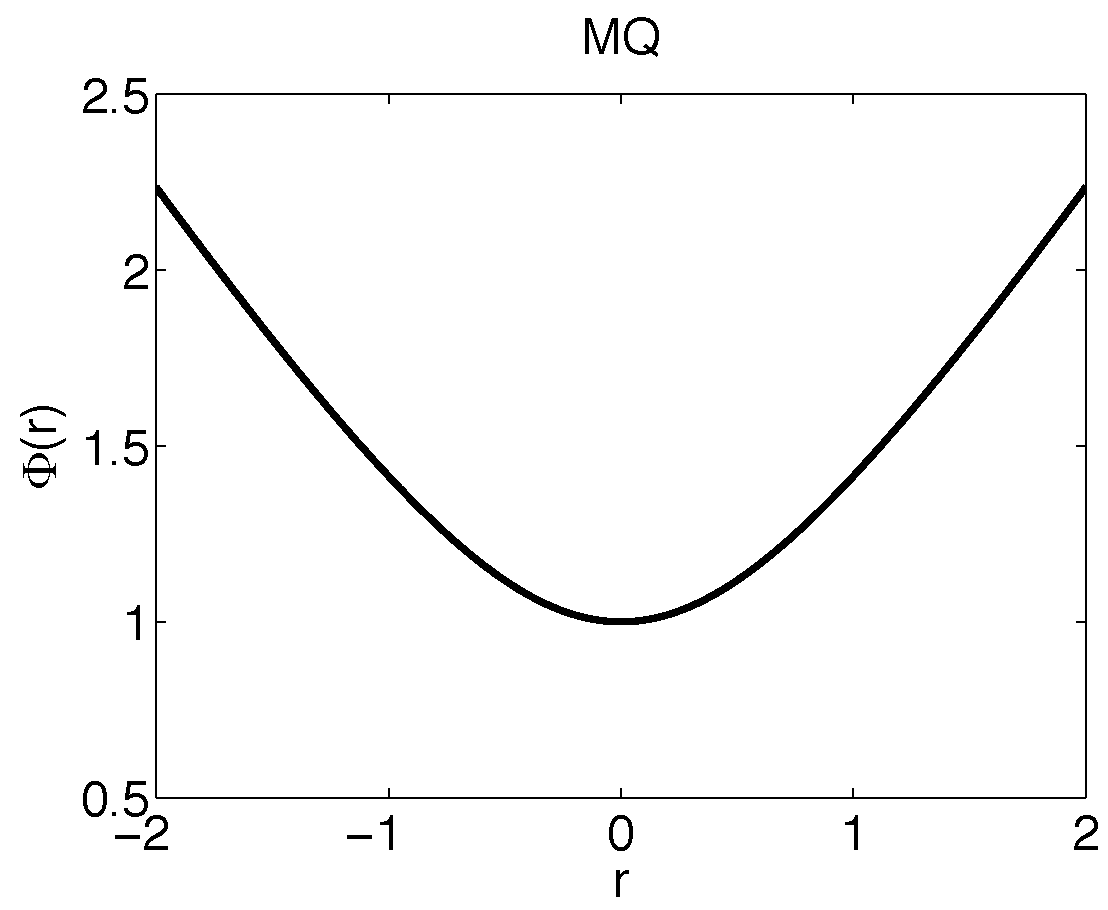
\includegraphics[width=0.25\textwidth]{matlab/mq_rbf.pdf}   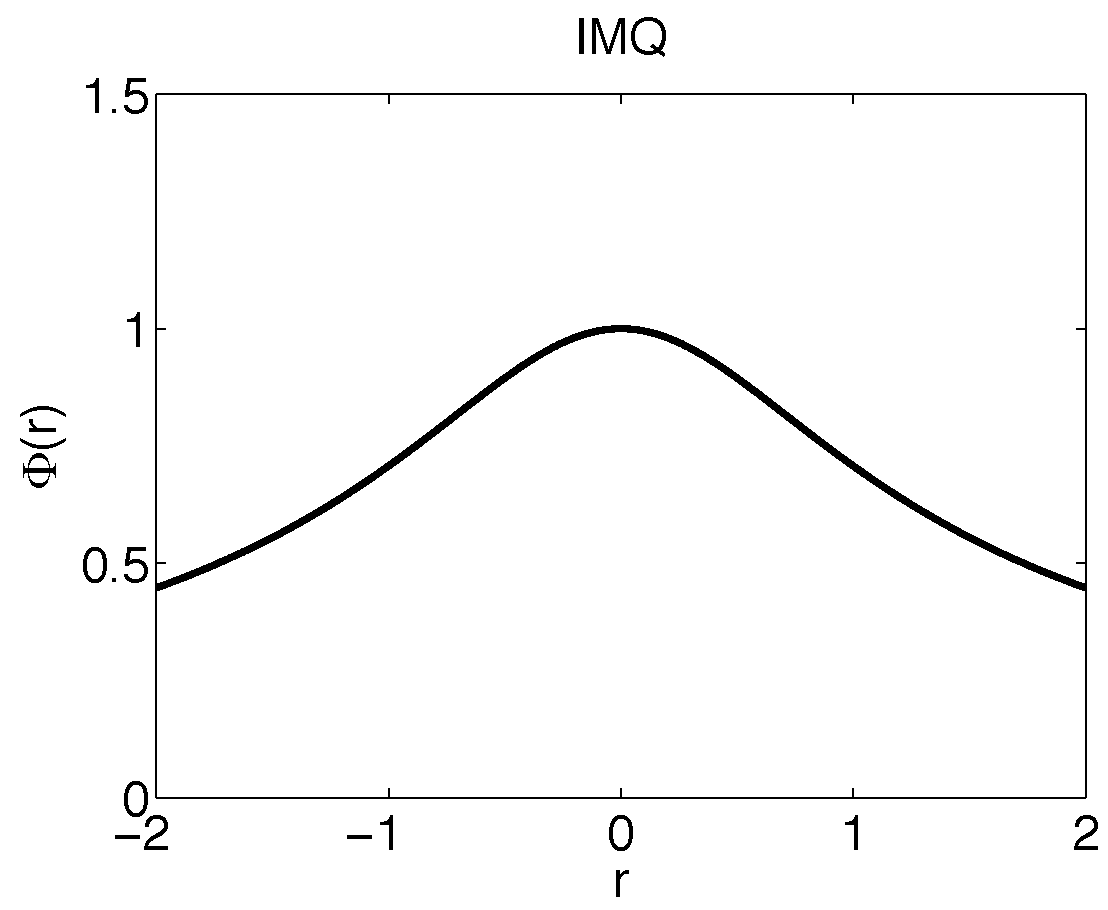
\includegraphics[width=0.25\textwidth]{matlab/imq_rbf.pdf} 
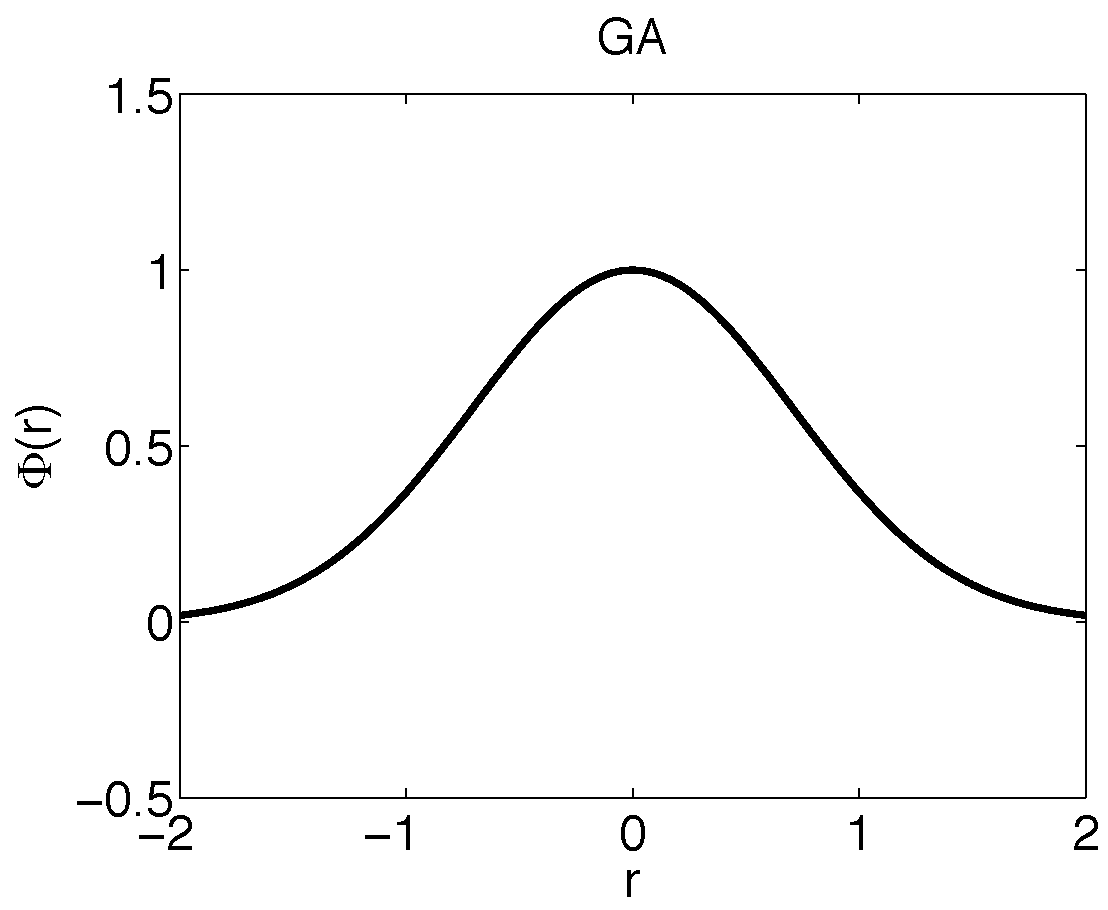
\includegraphics[width=0.25\textwidth]{matlab/ga_rbf.pdf} \\  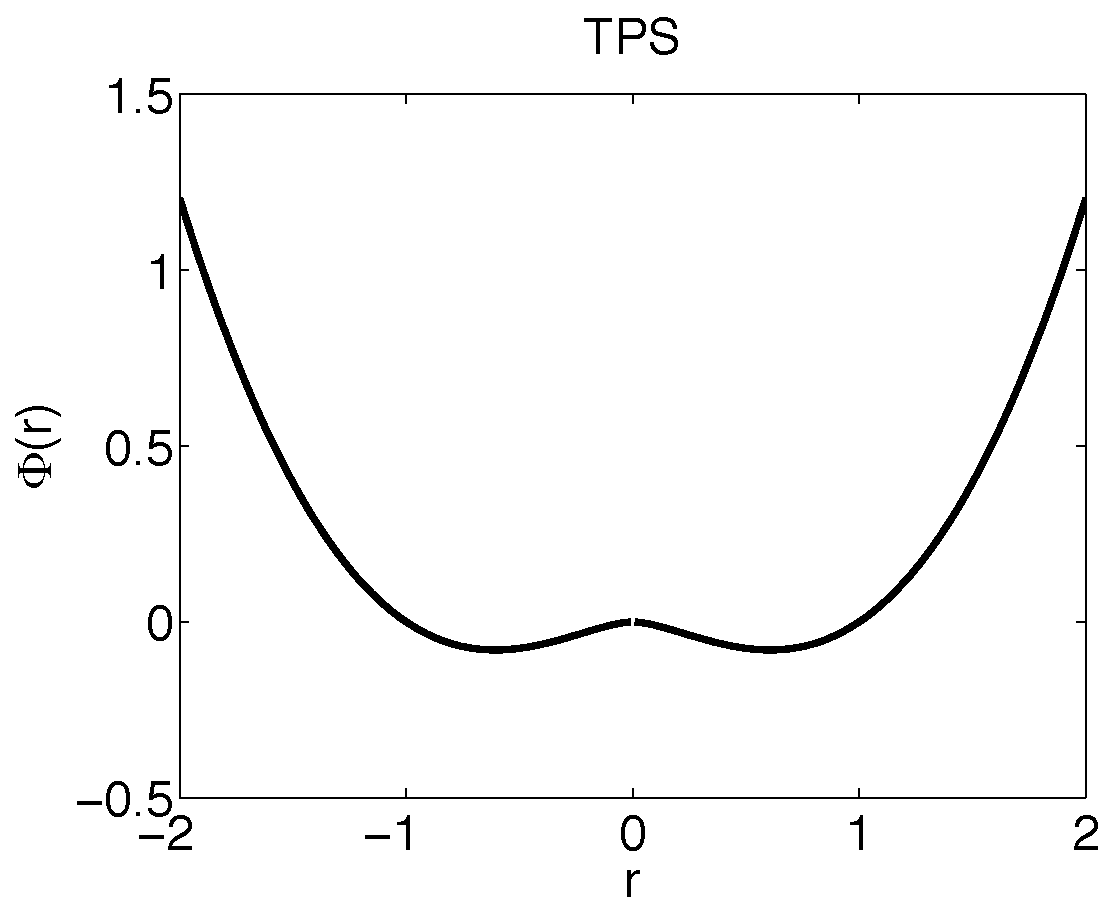
\includegraphics[width=0.25\textwidth]{matlab/tps_rbf.pdf} 
%\end{tabular} \\
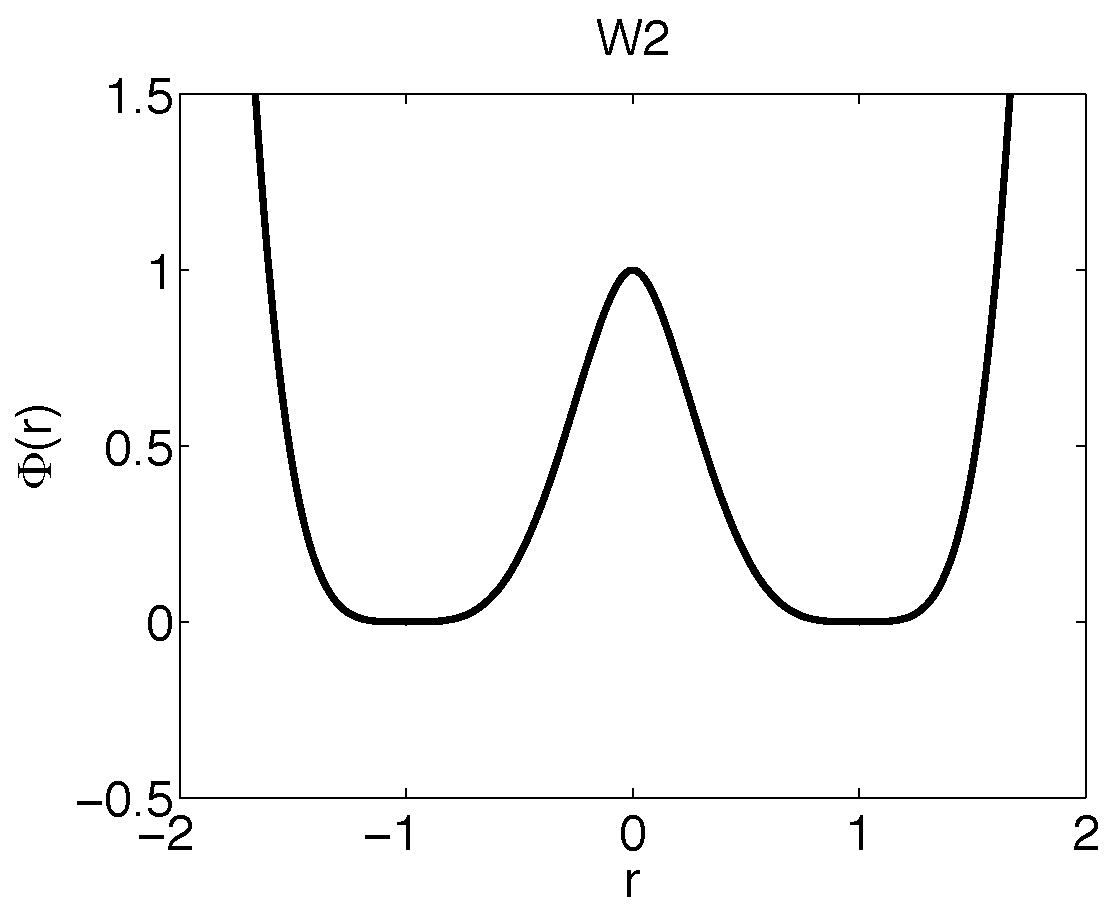
\includegraphics[width=0.25\textwidth]{matlab/w2_rbf.pdf}
\caption{Example RBF shapes from Table~\ref{tbl:rbfs} with parameter $\varepsilon=1$.}
\label{fig:rbf_examples}
\end{figure} 


\begin{figure}[t]
\centering
\begin{tabular}{cc}
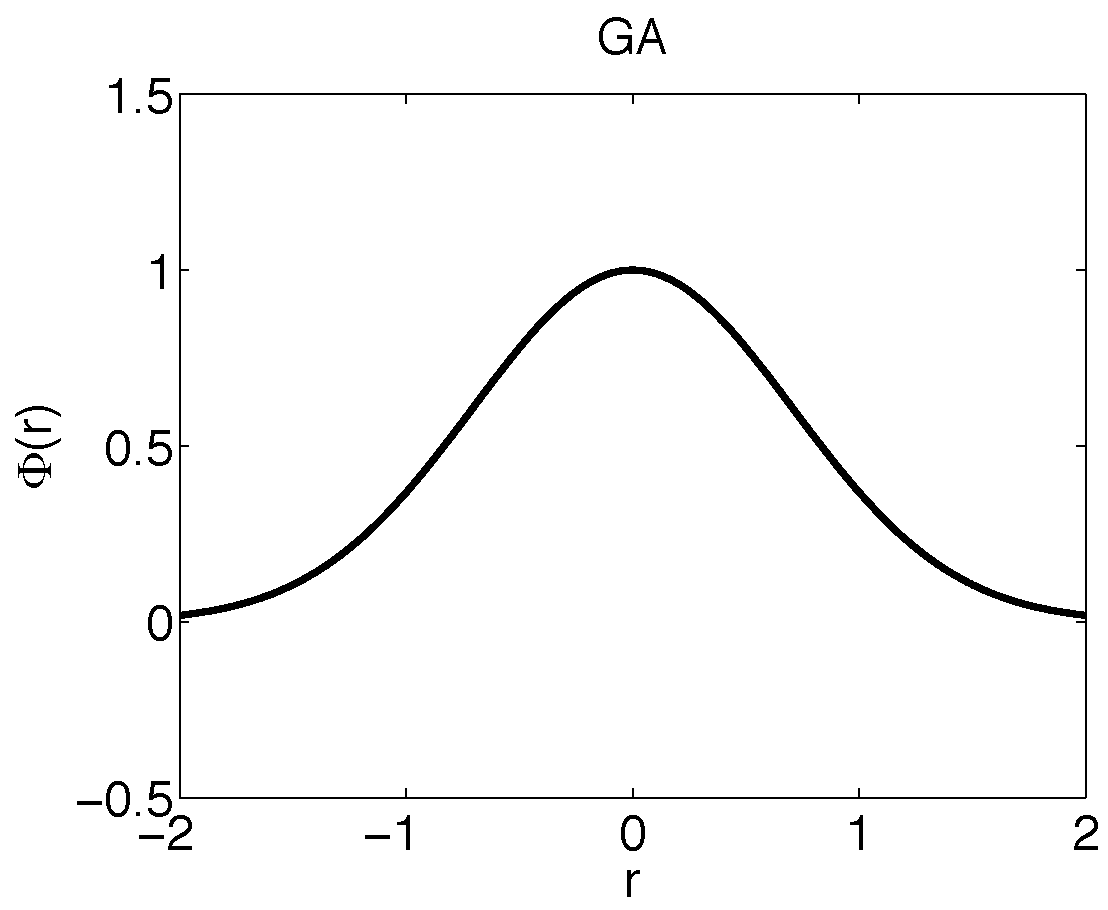
\includegraphics[width=0.25\textwidth]{matlab/ga_rbf.pdf}
\includegraphics[width=0.35\textwidth]{matlab/ga_rbf2D.eps}
\includegraphics[width=0.35\textwidth]{matlab/ga_rbf3D.eps}
\end{tabular} 
\caption{The Gaussian (GA) RBF (Table~\ref{tbl:rbfs}) with parameter $\varepsilon=1$ in dimensions 1, 2 and 3.}
\label{fig:rbf_dimension_example}
\end{figure} 

\begin{figure}[t]
    \centering
    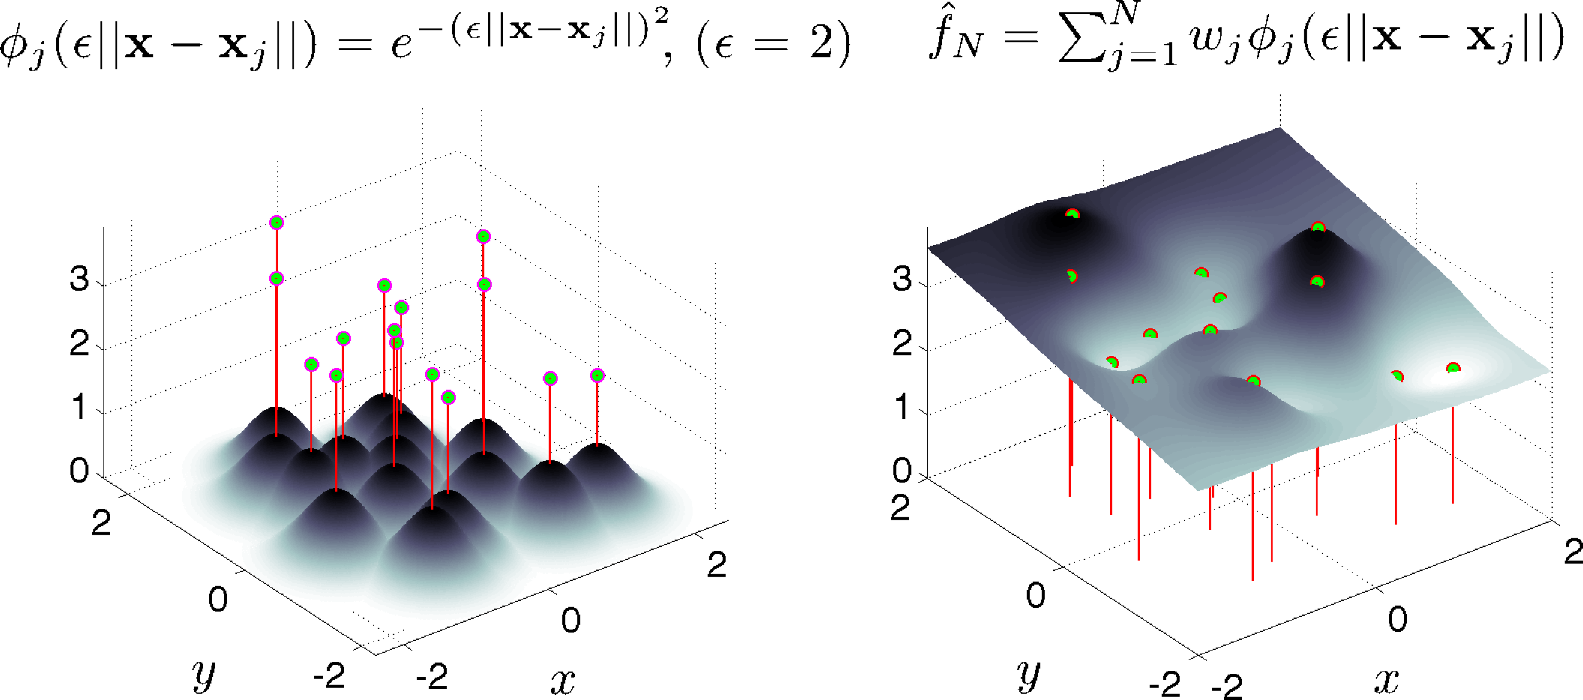
\includegraphics[scale=0.4]{figures/trimmed_interpolate2D_ga__m.pdf}
    \caption{RBF interpolation using 15 translates of the Gaussian RBF with $\epsilon=2$. One RBF is centered at each node in the domain. Linear
    combinations of these produce an interpolant over the domain passing through known function values. }
    \label{fig:rbfInterpolation}
\end{figure}

%TODO: expand with new literature since 2009
%TODO: any new methods?


RBF methods for interpolation first appeared in 1971 with Hardy's seminal research on multiquadrics
\cite{Hardy1971}. In his 1982 survey of scattered data interpolation methods \cite{Franke1982}, Franke rated multiquadrics first-in-class against 28 other methods (3 of which were RBFs) \cite{Franke1982}. Many other RBFs, 
including those presented in Table~\ref{tbl:rbfs} have been applied in literature, but for PDEs in particular, none have rivaled the 
attention received by multiquadrics. 


By 1990, the understanding of the scientific community regarding RBFs was sufficiently developed for collocating PDEs \cite{Kansa1990a,Kansa1990b}. PDE collocation seeks a solution of the form
\begin{eqnarray*}
(\diffop{u})(x_i) = \sum_{j=1}^{N} \phi_j(x_i) c_j = f(x_i)
\end{eqnarray*}
where $\diffop{}$ is, in general, a nonlinear differential operator acting on $u(x)$. The solution $u(x)$ is expressed as a linear combination of $N$ basis functions $\phi_j(x)$, not necessarily RBFs: 
$$
u(x) = \sum_{i=1}^N \phi_j(x) c_j 
$$
As in the problem of RBF scattered data interpolation, $ \vc = \{c_j\} $ is the unknown coefficient vector. 
Under the assumption that $\mathcal{L}$ is a linear operator, one can collocate the differential equation. Alternatively, individual derivative operators can be expressed as linear combinations of the unknowns $u_j$ (leading to the RBF-FD methods). 
In all cases, a linear system of equations arises, with different degrees of sparsity, dependent on the chosen basis functions and how the various constraints are enforced.  While we restrict the $\phi_j(x)$ to RBFs or various operators applied to the RBFs, we note that spectral methods, finite-element or spectral-element methods can be formulated in a similar way with different choices of basis functions.  Of course, $u$ can be a vector of unknown variables ($\vc$ then becomes a matrix). 

In Table~\ref{tbl:rbfcolloctypes} we classify references according to their choice of collocation method and RBF 
interpolation type. 
There are three main categories of RBF interpolation; we list them in Table~\ref{tbl:interp_types}. The first is \emph{Global} in the case that a single, large ($N\times N$) and 
dense matrix corresponding to globally supported RBFs is inverted; second, \emph{Compact} if compactly supported RBFs are used to 
produce a single, large, but \emph{sparse} matrix; and third, \emph{Local} if compactly supported RBFs are used to produce many small but 
dense matrices with one corresponding to each collocation point. In all three cases the matrices are symmetric and with the correct choice of RBF they are at least conditionally positive definite. The final row of Table~\ref{tbl:rbfcolloctypes} considers literature on the RBF-FD method and is discussed in depth in Chapter~\ref{chap:rbffd_method}.

\begin{table}[t]
   \centering
   \begin{tabular}{E | C | C | C | c | } % Column formatting, @{} suppresses leading/trailing space
   Interpolation Type & Dense/Sparse $A$ & Dim($A$) ($N_S \ll N$) &  \# of $A^{-1}$  & RBF Support \\ 
   \hline \hline
   Global & Dense & $N \times N$ & 1 & Global \\
   Compact & Sparse & $N \times N$ & 1 & Compact \\
   Local & Dense & $N_S \times N_S$ & N & Global/Compact
   \end{tabular}
   \caption{RBF interpolation types and properties, assuming a problem with $N$ nodes.}
   \label{tbl:interp_types}
\end{table}


We note that three types of collocation occur throughout the RBF literature: 
Kansa's unsymmetric collocation method \cite{Kansa1990a, Kansa1990b}, Fasshauer's symmetric collocation method \cite
{Fasshauer1997}, and the Direct collocation method \cite{Fedoseyev2002}. 
%TODO: classify RBF-PS applications

% While not a collocation method, RBF-FD represents the latest trend in solving PDEs with RBFs.  %A full explanation of RBF based collocation is deferred to Chapter~\ref{chap:rbf_pde}. 

We now turn to discussion of the benefits and shortcomings of each RBF method, before covering derivation of the methods. 
%Prior to launching into derivation each RBF collocation method, we first survey the classifications to highlight benefits, shortcomings, and to provide a brief historical context. A survey of related work in the RBF community that involves parallelization and optimization is deferred to Chapter~\ref{chap:parallel_rbf}. 

\subsection{Global RBF Methods}

\emph{Kansa's method} \cite{Kansa1990a, Kansa1990b} (a.k.a. unsymmetric collocation) was the first RBF method for PDEs, and is still the most frequently used method. The idea behind Kansa's method is that an 
approximate solution to the PDE can be found by finding an interpolant which satisfies the differential operator with zero residual at a set of \emph{collocation points} (these coincide with the RBF centers). To find the interpolant, the differential equation is formulated as a two block (unsymmetric) linear system with: 1) the approximation of values 
at boundary 
points with boundary data only, and 2) the approximation of interior points by directly applying the differential operator. It was 
shown in \cite{Fasshauer1997, Hon2001} that the unsymmetric linear system produced by Kansa's method does not guarantee 
non-singularity; although it is also noted that in practice singularities are rare encounters \cite{Larsson2003}. 

The second alternative for RBF collocation, is based on Hermite scattered 
data interpolation (see \cite{Wu1992}). The so-called \emph{Fasshauer} or \emph{Symmetric Collocation} method (\cite{Fasshauer1997}) 
performs a change of basis for the interpolant by directly applying the differential operator to the RBFs. It then collocates using the same approach as Kansa's method \cite{Stevens2009b, Larsson2003}. The resulting block structure of the linear system is symmetric and 
guaranteed to be non-singular \cite{Fasshauer1997}. In comparison to Kansa's method, the disadvantages of Fasshauer's method 
include: a) requirement of higher order differentiability of the basis functions (to satisfy double application of the differential operator)
% it has stronger regularity assumptions (it is Hermite interpolation), 
and b) the linear system is larger and more complex to form
%, and c) it is not ideally suited for non-linear problems
 \cite{Fasshauer2007}. As \cite{Hon2001} points out, 
the possible existence of a singularity in Kansa's method is not enough to justify the added difficulties of using Fasshauer's 
method.

%TODO: refs that refer to global RBF methods and RBF-PS as just RBF methods. 

The last collocation method, \emph{Direct Collocation}, was introduced by Fedoseyev, Friedman and Kansa
 \cite{Fedoseyev2002} and satisfies the differential operator on the interior and the boundary. Larsson and Fornberg \cite{Larsson2003} observe that this third method has a matrix structure similar to that found in Kansa's method; however, it is noted that the dimensions of the matrix blocks for each method differ. This is due to collocation constraints added for 
the differential operator applied to the boundary. Aside from the survey on RBF collocation presented by Larsson and Fornberg \cite{Larsson2003}, no related 
work was found that applied, or investigated, this method further.  

Both Kansa's method and Fasshauer's methods were shown in \cite{Fasshauer2006} to fit well in the generalized framework of pseudo-spectral methods with a subtle change in algorithm. While collocation methods explicitly compute the coefficients for a continuous derivative approximation, their alternates, referred to in literature as RBF-pseudospectral (RBF-PS) methods, never explicitly compute the interpolant coefficients. Instead, a differentiation matrix (DM) is assembled and used to approximate derivates at the collocation points only \cite{FasshauerZhang2007}. Since most computational models are simply concerned with the solution at collocation points, the change to assemble DMs as in RBF-PS is organic. 


Following the evolution of the RBF-PS algorithm, applications of global RBFs in the classic collocation sense (i.e., without the RBF-PS DMs) become impractical. This statement stems from the algorithmic complexity of each method. 
%As discussed in \cite{Fasshauer2007, FlyerWright09}, RBF methods result in matrices that are full. The 
Global RBF methods result in full matrices \cite{Fasshauer2007}. The global collocation methods then scale on the order of $O(N^3)$ floating point operations (FLOPs) to solve for weighting coefficients on a given node layout, plus $O(N^2)$ to apply the weights for derivatives. If time-stepping is required, global collocation methods must recompute the time-dependent coefficients with additional cost dominated by $O(N^3)$ operations. RBF-PS methods have similar requirements for $O(N^3)$ operations to assemble the differentiation matrix and $O(N^2)$ to apply for derivatives. However, by avoiding time-dependent coefficients, RBF-PS methods only apply the differentiation matrix each time-step for $O(N^2)$ operations. As an aside, the $O(N^3)$ complexity for each method---typically due to an LU-decomposition, with subsequent forward- and back-solves---could be reduced. While not in mainstream use by the RBF community, \cite{Morse2005} correctly points out that the use of iterative solvers could reduce complexity of preprocessing to the order of $O(N^2)$. 
%For mid- to large-scale problems, in the unlikely event that conditioning of the system is not a limiting factor, the cost of the method is still seen as prohibitively high. 

Hon et al. \cite{Hon1999} employed Kansa's method to solve shallow water equations for Typhoon simulation.
In \cite{FlyerWright09}, Flyer and Wright employed RBF-PS (Kansa method) for the solution of shallow water equations on a sphere. Their 
results show that RBFs allow for longer time steps with spectral accuracy. The survey \cite{FlyerFornberg11} by Flyer and Fornberg showcases RBF-PS (Kansa) out-performing some of the of the best available methods in geosciences, namely: Finite Volume, Spectral Elements, Double Fourier, and Spherical Harmonics. When applied to problems such as transport on the sphere \cite{FlyerWright07}, shallow water equations \cite{FlyerWright09}, and 3D mantle convection\cite{WrightFlyerYuen10}, RBF-PS consistently required fewer time steps, and a fraction of the nodes for similar accuracy \cite{FlyerFornberg11}. 
%TODO: add \cite{Neves2009}

%
%In the survey on RBF collocation presented by Larsson and Fornberg \cite{Larsson2003}, it was found that performance of the 
%collocation methods depends on the choice of RBFs (i.e., whether they are infinitely smooth or piecewise smooth). Their end 
%conclusion, however, was that infinitely smooth RBFs are preferred for Elliptic PDEs as they do not require node placement 
%optimization.

%Kansa collocation
\newcommand{\kansaglobalrbf}[0]{\cite{Kansa:1990a, Kansa:1990b, Fasshauer:2006, Fornberg:2004, Mouat:2002, Hon:2001, Franke:1982, Flyer:2009b, Flyer:2007, Hon:1999, Fornberg:2008, Larsson:2003}}
\newcommand{\kansacsrbf}[0]{\cite{Fornberg:2008, Wang:2002}}
\newcommand{\kansalocalrbf}[0]{\cite{Divo:2007, Kosec:2008, Sarler:2006, Vertnik:2006}}

% Fasshauer collocation
\newcommand{\fassglobalrbf}[0]{\cite{Fasshauer:2006, Fasshauer:1997, Larsson:2003}}
\newcommand{\fasscsrbf}[0]{\cite{Liu:2005}}
\newcommand{\fasslocalrbf}[0]{\cite{Stevens:2008a, Stevens:2009a, Stevens:2009b}}

% Direct collocation
\newcommand{\directglobalrbf}[0]{\cite{Fedoseyev:2002, Larsson:2003}}
\newcommand{\directcsrbf}[0]{}
\newcommand{\directlocalrbf}[0]{}


% RBF-FD
\newcommand{\rbffdglobalrbf}[0]{N/A}
\newcommand{\rbffdcsrbf}[0]{N/A}
\newcommand{\rbffdlocalrbf}[0]{\cite{Wright:2006,Wright:2003, Shu:2003, Cecil:2004, Wright:2004, Shu:2006, Chandhini:2007}}


%\begin{sidewaystable}
\begin{table}[t]
\begin{center}
	\begin{tabular}{@{} R|C|C|C|}
		& \multicolumn{3}{c|}{RBF Interpolation Type} \\
		\hline
		Method & Global (Dense) & Compact (Sparse Global) & Local \\
		\hline \hline
		Kansa's Method &\kansaglobalrbf & \kansacsrbf & \kansalocalrbf \\
		\hdashline
		Fasshauer's Method &\fassglobalrbf & \fasscsrbf & \fasslocalrbf \\
		\hdashline
		Direct Collocation &\directglobalrbf & \directcsrbf & \directlocalrbf \\
		\hdashline
		RBF-FD & \rbffdglobalrbf & \rbffdcsrbf & \rbffdlocalrbf \\
		\hline
	\end{tabular}
\end{center}
\caption{Classification of references based on choice of RBF interpolation types and method for solving PDEs. References may appear in multiple cells according to the breadth of their research.}
\label{tbl:rbfcolloctypes}
\end{table}
%\end{sidewaystable}




\subsection{Compactly Support RBFs} 

Thus far, all cases of collocation and interpolation mentioned have assumed globally supported RBFs. While global RBFs are well-studied and have nice properties, a major limitation is the large, dense system that must be solved. One alternative to global support is to use a set of compactly supported RBFs (CSRBFs) that are defined as: 
\begin{equation}
\phi(r) = \begin{cases} \varphi(r) & r \in [0,1]\\
0 & r > 1
\end{cases}
\label{eqn:csrbf}
\end{equation}
where a cut-off radius is defined past which the RBF (in this case $\varphi(r)$) has no influence on the interpolant. Note that the radius can be scaled to fit a desired support. Methods that leverage CSRBFs produce a global interpolation matrix that is \emph{sparse} and therefore results in a system that is more efficiently assembled and solved with smaller memory requirements \cite{Fasshauer2007}. The actual complexity estimate of the CSRBF method depends on the sparsity of the problem as well as the ordering of the assembled system. Assuming $n \ll N$ where $n$ represents the number of nodes in support, \cite{Zhang2004} lists the complexity as dominated by $O(N)$ for properly structured systems within MATLAB, and the investigation in \cite{Morse2005} found $O(N^{1.5})$ consistent with the estimate provided by their choice of general sparse solver package. A multi-level CSRBF method, introduced by Fasshauer \cite{Fasshauer2007}, collocates solutions over multiple grid refinements to achieve reduced $O(N)$ complexity, but the method is plagued by poor convergence. We also notes that in the context of CSRBFs, analogues to Kansa's method and Fasshauer's method are known by the names \emph{radial point interpolation method (RPIM)} \cite{Wang2002} and \emph{radial point interpolation collocation method (RPICM)} \cite{Liu2005}, respectively. A more thorough survey of CSRBF history can be found in \cite{Fasshauer2007,Iske2004}.

CSRBFs have attracted a lot of attention in applications. For example, in the field of dynamic surface and image deformation, compact support allows for local transformations which do not induce global deformation (see e.g., \cite{Yang2008, Lin2009, Correa2007}). 




\subsection{Local RBF Methods}
% TODO: review these papers
Around 2005, \v{S}arler and Vertnik \cite{Sarler2006, Vertnik2006} demonstrated that if compactly supported RBFs are chosen, the traditional global 
collocation matrix from Kansa's method, can be avoided altogether in favor of small localized collocation matrices defined for 
each node. Local collocation still faces possible ill-conditioning and singularities 
like global collocation, but make it easier to distribute computation across parallel systems. Also, the smaller linear systems can be 
solved 
with less conditioning issues. In \cite{Sarler2006}, the authors consider 2D diffusion problems. Divo and Kassab \cite{Divo2007} 
employ the 
method for Poisson-like PDEs including fluid flow and heat transfer. Kosec and \v{S}arler \cite{Kosec2008} apply the 
same technique to solve coupled heat transfer and fluid flow problems.

In similar fashion, Stevens et al. \cite{Stevens2009a} introduced a local version of 
Fasshauer's method called \emph{local Hermitian interpolation}. The authors have applied their method to 3D soil 
problems based on transient Richards' equations \cite{Stevens2008a, Stevens2009a, Stevens2009b}.


\subsection{Recent Advances in Conditioning}

The most limiting factor in the success of RBF methods is not the complexity of the methods, nor the task of collocating the PDE. Rather, it is the support parameter, $\epsilon$, and the dilemma one faces in the \emph{Uncertainty Relation} \cite{Schaback1995}. Recall that as $\epsilon \rightarrow 0$ ill-conditioning increases, but the accuracy of the method also increases. Similarly, as the number of collocation points increases, so too does the ill-conditioning. 

In response to this problem, Fornberg and Wright 
\cite{Fornberg2004} presented the \emph{Contour--Pad\'{e} algorithm}, which allows for numerically stable 
computation of highly 
accurate interpolants for (very small) cases typically associated with ill-conditioning induced by nearly flat RBFs (i.e., $\epsilon \rightarrow 0$). Larsson and Fornberg \cite{Larsson2003} 
applied the 
algorithm to all three methods of collocation (Kansa's, Fasshauer's and Direct Collocation) with considerable gain in accuracy over solutions from classical second-order FD and a pseudospectral method. %TODO: verify 
Note that currently, the Contour-Pad\'{e} 
algorithm was only studied for global RBF interpolation, not for compact or local collocation methods. 

The \emph{RBF-QR} method, an alternative for numerically stable computation in the limit as $\epsilon \rightarrow 0$, was introduced by Fornberg  and 
Piret \cite{Fornberg2007} in context of a sphere, and later extended to planar 2D problems in \cite{Fornberg2009b}. The 
RBF-QR 
method is simple 
to implement (less than 100 lines of Matlab code), and it allows solution of large problems that are typically ill-conditioned. Fornberg, Larsson and Flyer \cite{Fornberg2009b} successfully applied RBF-QR on large problems with 6000 nodes for globally supported basis functions. 
%TODO: add mention of bengt's latest on RBF-QR \cite{Fornberg2011a, Fornberg2011b}

With these two algorithms, global RBF methods have overcome most ill-conditioning issues for small to mid-sized problems. Unfortunately, both Contour-Pad\'{e} and RBF-QR fail for large problems.
% due to ill-conditioning. 
As the number of RBFs increases beyond a few thousand nodes it is impossible to avoid  ill-conditioning of the extremely large interpolation matrix.

This reveals the benefit of local methods, which decrease the number of RBFs and ill-conditioning. However, in the limit as local stencil size increases to include all nodes in a domain, the local and global method are equivalent; thus it is known that local methods also suffer extreme ill-conditioning around 2000 nodes per stencil \cite{Shu2006}. Although, to our knowledge, no applications of local methods require more than a few hundred nodes per local solution. 

 


%To our our knowledge, no research has yet been published that applies the RBF-QR method to RBF-FD stencils.

%
%In 2002, Mouat and Beatson \cite{Mouat2002} suggested that Matern functions would be more accurate than the more 
%commonly chosen multiquadrics. 
%The authors also considered the problem of a large number of nodes with a discussion of a 
%domain decomposition method for PDE solution. 


\section{Comparison of RBF Methods}

We now detail RBF methods for PDEs leading up to the derivation of RBF-FD. 

Following \cite{Mouat2002}, consider a PDE expressed in terms of a (linear) differential operator, $\diffop$: 
\begin{eqnarray*}
\diffop{u} & = & f \on{\Interior} \\
u &=& g \on{\Boundary}
\end{eqnarray*}
where $\Interior$ is the interior of the physical domain, $\Boundary$ is the boundary of $\Interior$ and $f,g$ are known explicitly. In the case of a non-linear differential operator, a Newton's iteration, or some other method, can be used to linearize the problem (see e.g., \cite{WrightFornberg06}); of course, this increases the complexity of a single time step. Then, the unknown solution, $u$, which produces the observations on the right hand side can be approximated by an interpolant function $u_{\phi}$ expressed as a linear combination of radial basis functions, $\{\phi_j(x) = \phi(\vectornorm{x-x_j})\}_{j=1}^{N}$, and polynomial functions$\{P_l(x)\}_{l=1}^{M}$:
\begin{equation}
	u_{\phi}(x) = \sum_{j=1}^{N}  \phi_j(x) c_{j} + \sum_{l=1}^{M}  P_l(x) d_{l}, \hskip1.5em P_l(x) \in \Pi^{d}_{p}
	\label{eqn:pde_approx}
\end{equation}
where $\phi_j(x) = \vectornorm{x - x_j}_2$ (Euclidean distance). The 
second sum represents a linear combination of polynomials that enforces zero approximation error
 when $u(x)$ is a polynomial of degree less than or equal to $p$. The variable $d$ is the 
 problem dimension (i.e., $u_{\phi}(x) \in \R^{d}$). 
%\toevan{Finish to end of paragraph} 
To eliminate degrees of freedom for well-posedness, $p$ should be greater than or equal to the order of the chosen RBF
 (see Table~\ref{tbl:rbfs}) \cite{Iske2004}.  
Note that Equation~\ref{eqn:pde_approx} is evaluated 
 at $\{x_j\}_{j=1}^{N}$ 
data points through which the interpolant is required to pass with zero residual.  We refer to 
the $x_j$'s as \emph{collocation points} (a.k.a. trial points), taken as the RBF centers. The test points, $x$, usually coincide with collocation points, although this is not a requirement. 
%$P_l(x)$ is needed to eliminate degrees of freedom for well-posedness \cite{Iske:2004}. 

To clarify the role of the polynomial part in Equation~\ref{eqn:pde_approx}, it is necessary to
put aside the PDE for the moment and consider only the problem of \emph{scattered data 
interpolation} with Radial Basis Functions.

\subsection{RBF Scattered Data Interpolation}
 Borrowing notation from \cite{Fasshauer2007, Iske2004}, 
we seek an interpolant of the form
\begin{eqnarray*}
f(x) = \sum_{j=1}^{N} \phi_j(x) c_{j}  \label{eq:rbf_scattered_data_interp}
\end{eqnarray*}
where $f(x)$ is expressed as a scalar product between the unknown coefficient weights $c_j$ and the radial basis functions $\phi_j(x)$.

To obtain the unknown coefficients, $c_j$, form a linear system in terms of the $N$ RBF centers:
\begin{eqnarray*}
f(x) & = & \sum_{j=1}^{N} c_{j}  \phi_j(x)  \hskip1.5em \textrm{for\ } x = \{x_j\}_{j = 1}^{N} \\
 \parray{c}{ f } & =&  \barray{c}{\phi}\parray{c}{ c } 
\end{eqnarray*}
The invertibility of this system depends on the choice of RBF, so one typically chooses a function that is positive definite to avoid issues. It has been shown (see \cite{Fasshauer2007, Iske2004}) that some choices of RBFs (e.g. multiquadrics and thin-plate splines \cite{Hon2001}) are not positive definite and therefore there is no guarantee that the approximation is well-posed. A sufficient condition for well-posedness is that the matrix be \emph{conditionally positive definite}. In \cite{Fasshauer2007}, Fasshauer demonstrates that conditional positive definiteness is guaranteed when Equation~\ref{eqn:pde_approx} exactly reproduces functions of degree less than or equal $m$. 
For RBF scattered data interpolation in one dimension, this can be achieved by adding a polynomial of order $m$ with $M =$${m+1}\choose{1}$ terms (e.g., $x^0, x^1, \cdots, x^{m}$). 
%For $\R^2$, the terms would be: $1, x, y, xy, x^2y, xy^2, \cdots, x^{m}y^{m-1}, x^{m-1}y^{m}, x^my^m$. 
In $\R^d$, $M =$${m+d}\choose{d}$ \cite{Iske2004}, giving
\begin{eqnarray}
\sum_{j=1}^{N} c_{j}  \phi_j(x)  +  \sum_{l=1}^{M} d_{l} P_l(x) & = & f(x),  \hskip1.5em  P_l(x) \in \Pi^{d}_{m} \label{eqn:interpolation_constraints} \\
\left[ \begin{array}{c c} 
	\phi & P
	\end{array} \right] \left( \begin{array}{c}
							c \\
							d
							 \end{array}
						 \right) & = & \parray{c}{ f } \nonumber
\end{eqnarray}
where the second summation (referred to as \emph{interpolation conditions} \cite{Iske2004}) ensures the minimum degree of the interpolant. Refer to Table~\ref{tbl:rbfs} for a short list of recommended RBFs and minimally required orders of $m$. This document prefers the Gaussian RBF. Notice, in Equation~\ref{eqn:interpolation_constraints}, that the interpolation conditions add $M$ new degrees of freedom, so we must provide $M$ 
additional constraints to square the system. In this case:
$$
\sum_{j=1}^{N} c_{j} P_l(x_j) = 0,  \hskip1.5em  l=1,..., M 
$$
or 
\begin{eqnarray}
P^T {c}  = {0}. 
\label{eqn:extra_constraints}
\end{eqnarray}
It is now possible again to write the interpolation problem as a complete linear system using Equations~\ref{eqn:interpolation_constraints} and ~\ref{eqn:extra_constraints}:%as
\begin{eqnarray}
 \underbrace{\left[ \begin{array}{c c} 
	\phi & P \\
	P^T & 0
	\end{array} \right]}_{A} \left( \begin{array}{c}
							c \\
							d
							 \end{array}
						 \right) = \left( \begin{array}{c}
							f \\
							0
							 \end{array}
						 \right) \label{eq:solve_rbf_scattered_interp}
\end{eqnarray}
%This system then produces coefficients capable of exactly approximating data from polynomials of degree less than or equal to $m$ \cite{Fasshauer2007}. 
Equation~\ref{eq:solve_rbf_scattered_interp}---typically a dense system except in the case of RBFs with compact support---can be solved efficiently via standard methods like LU-decomposition.  With the coefficients, the interpolant can be sampled at any test points, $\{x_i\}_{i=1}^{n}$, by substitution into Equation~\ref{eq:rbf_scattered_data_interp}:
\begin{eqnarray}
f(x_i) & = & \sum_{j=1}^{N} c_{j}  \phi_j(x_i) +  \sum_{l=1}^{M} d_{l} P_l(x_i)  \nonumber \\
 & = & \left. \underbrace{\left[ \begin{array}{c c} 
       \phi &  P
	\end{array} \right]}_{B} 
	  \left( \begin{array}{cc}  c \\ d  \end{array} \right) \ \right|_{x={x_i}}
	\label{eqn:interpolate_x}
\end{eqnarray}


\subsection{Reconstructing Solutions for PDEs}
In the next few subsections, we will consider collocation equations based on this general form: 
\begin{eqnarray*}
\diffop{u_\phi(x)} &=& f(x) \on{\Interior} \label{eqn:colloc_interior}\\ 
\boundop{u_\phi(x)} &=& g(x) \on{\Boundary}  \label{eqn:colloc_boundary} 
\end{eqnarray*}
where the methods presented below will apply the differential operators, $\diffop{}$ and $\boundop{}$, to different choices of $u_\phi$ and different sets of collocation points. In many applications $\diffop{}$ is chosen as a differential operator (e.g., $\pd{}{x}$, $\nabla$, $\nabla^2$) and $\boundop = I$ (i.e. identity operator for Dirichlet boundary conditions) for PDEs. For RBF scattered data interpolation, $\diffop{} = I$. There are also  applications where $\diffop{}$ is a convolution operator (see e.g., \cite{Carr2001, Carr2003}) capable of smoothing/de-noising a surface reconstructed from point clouds. 

%TODO: label x_j's as TRIAL and x_is as TEST points
%\section{Approximating the Solution}
For all the methods that follow a linear system is generated: 
$$
A_{\diffop{}}  \left( \begin{array}{cc}  c \\ d  \end{array} \right)  =  \left( \begin{array}{cc}  f \\ 0  \end{array} \right) 
$$
\begin{equation}
  \left( \begin{array}{cc}  c \\ d  \end{array} \right) = A^{-1}_{\diffop{}}  \left( \begin{array}{cc}  f \\ 0  \end{array} \right) \nonumber
  %\label{eqn:solve_coeffs}
 \end{equation}
 where matrix $A_{\diffop{}}$ depends on the choice of collocation method. 
 % TODO: fix use of A_diffop; "but contains $\diffop{\phi} = \phi_\diffop{}$. 
Once the linear system is solved, the value $u(x)$ is reconstructed at the test points following Equation~\ref{eqn:interpolate_x}:
\begin{eqnarray}
u(x) & \approx &  \left.
\left[ \begin{array}{c c} 
       \phi &  P
	\end{array} \right]
	  \left( \begin{array}{cc}  c \\ d  \end{array} \right)  \ \right|_{x={x_i}} \nonumber\\
	 & \approx & B A^{-1}_\diffop{} \left( \begin{array}{cc}  f \\ 0  \end{array} \right) 
	\label{eqn:solve_u}
\end{eqnarray}
Likewise, to obtain differential quantities we have: 
\begin{eqnarray*}
\diffop{u}(x) & \approx & \left.
\left[ \begin{array}{c c} 
       \phi_{\diffop{}} &  P_{\diffop{}}
	\end{array} \right]
	  \left( \begin{array}{cc}  c \\ d  \end{array} \right)  \ \right|_{x={x_i}} \\
  	 & \approx & B_{\diffop{}} A^{-1}_\diffop{} \left( \begin{array}{cc}  f \\ 0  \end{array} \right)
	\label{eqn:solve_uxx}
\end{eqnarray*}
%where $\phi_{\diffop}$ is the analytic RBF with 

%TODO: \subsection{Applying Methods for PDEs}
%TODO: \subsubsection{Explicit PDEs}
%TODO: \subsubsection{Implicit PDEs} 

%Here we substitute $B$ for test samples in Equation~\ref{eqn:solve_u} to get the reconstructed solution:
%\begin{eqnarray}
%u(x) = B A^{-1}_\diffop{} \left( \begin{array}{cc}  f \\ 0  \end{array} \right)
%	\label{eqn:solve_rbf}
%\end{eqnarray}
%where the vector-matrix inner product $(A A^{-1}_{\diffop{}})$ is a row-vector. Since the coefficient vectors ${c}$ and ${d}$ are the same for all $x_i$, we can group the evaluation of $\diffop{u(x_i)}$ for $i=1,...,n$ as a matrix-vector multiplication where the matrix rows correspond to $(A_\diffop{} A^{-1})$ for each $x_i$. 


%TODO: mention equation~\ref{eqn:solve_rbf} can be precomputed DM applied to f for collocation points in pseudo-spectral method.  
%Relevant to the discussion of RBF-PS and computational and memory efficient global RBF methods, if $A$ contains rows corresponding to the interpolation problem can be rewritten independent of coefficients by assembling a differentiation 
 
\subsection{PDE Methods} 

Now, since $u_{\phi}(x)$ from Equation~\ref{eqn:pde_approx} cannot (in general) satisfy the PDE everywhere, we enforce the PDE at a set of collocation points, which are  distributed over both the interior and the boundary. Again, these points do not necessarily coincide with the RBF centers, but it is convenient for this to be true in practice. Also, for each of the methods the choice of RBF can be either global, resulting in a large dense system, or compact, resulting in a large sparse system. 

\subsubsection{Kansa's Method}

The first global RBF method for PDEs, \emph{Kansa's method} \cite{Kansa1990a, Kansa1990b}, collocates the solution through known values on the boundary, while constraining the interpolant to satisfy the PDE operator on the interior. This is equivalent to choosing $u_\phi$ according to Equation~\ref{eqn:pde_approx}. The resulting system is given by \cite{Mouat2002}; assuming that $\diffop{}$ is a linear operator, 
\begin{eqnarray}
\diffop{u_\phi(x_i)} = \sum_{j=1}^{N}c_j\diffop{\phi_j(x_i)} + \sum_{l=1}^{M}d_l \diffop{P_l(x_i)} &=&f(x_i)  \hskip1.5em i = 1,...,n_I  \label{eqn:kansa_interior} \\ 
\boundop{u_\phi(x_i)} = \sum_{j=1}^{N}c_j \boundop{\phi_j(x_i)} + \sum_{l=1}^{M}d_l \boundop{P_l(x_i)} &=& g(x_i)  \hskip1.5em i = n_I + 1, \cdots, n \label{eqn:kansa_boundary} \\
\sum_{j=1}^{N} c_j P_l(x_j) & = & 0 \hskip3.0em l=1,\cdots,M \label{eqn:kansa_constraints} 
\end{eqnarray}
where $n_I$ are the number of interior collocation points, with the number of boundary collocation points equal to $n - n_I$. First, observe that the differential operators are applied directly to the RBFs inside summations, rather than first solving the scattered data interpolation problem and then applying the operator to the interpolant.  Second, since the basis functions are known analytically, it is possible (although sometimes painful) to derive $\diffop{\phi}$ (refer to \cite{Fasshauer2007} for RBF derivative tables); the same is true for the polynomials $P_l$. 

We can now reformulate Kansa's method as the linear system: 
\begin{eqnarray}
\underbrace{\left[ \begin{array}{c c} 
	\phi_\diffop{} & P_\diffop{} \\
	\phi_\boundop{} & P_\boundop{} \\
	P^T & 0
	\end{array} \right]}_{A_{\diffop{}}}  \left( \begin{array}{c}
							{c} \\
							{d}
							 \end{array}
						 \right) = \left( \begin{array}{c}
							{f} \\
							{g} \\
							0
							 \end{array}
						 \right) 
	\label{eqn:kansa_method}
\end{eqnarray}
% TODO: add underline stating that matrix is A. 


where $\phi_\diffop{} = \diffop{\phi}$, $P_\diffop{} = \diffop{P}$ are the interior components (Equation~\ref{eqn:kansa_interior}), $\phi_\boundop{}$ and $P_\boundop{}$ are the boundary components (Equation~\ref{eqn:kansa_boundary}), and $P^T = \left[P_\diffop{}^T \ \ P_\boundop{}^T\right]$ are constraints for both interior and boundary polynomial parts (Equation~\ref{eqn:kansa_constraints}). From Equation~\ref{eqn:kansa_method} it should be clear why Kansa's method is also known as the \emph{Unsymmetric} collocation method. 

%\toevan{Isn't $N+M=n$? For each case, you must put the proper relationships between $N$, $M$, $n_I$, $n$ so that the number of constraints equals the number of relations.}
Recall that the matrix in Equation~\ref{eqn:kansa_method} has no guarantee of non-singularity \cite{Fasshauer1997}; however, singularities are rare in practice \cite{Larsson2003}. 

\subsubsection{Fasshauer's Method}

\emph{Fasshauer's method} \cite{Fasshauer1997} addresses the problem of singularity in Kansa's method by assuming the interpolation to be Hermite. That is, it requires higher differentiability of the basis functions (they must be at least $C^k$-continuous if $\diffop{}$ is of order $k$). Leveraging this assumption, Fasshauer's method chooses: 
\begin{eqnarray}
u_\phi(x_i) & = & \sum_{j=1}^{N_I}  c_j \diffop{\phi_j(x_i)} + \sum_{j=N_{I} + 1}^{N} c_j \boundop{\phi_j(x_i)} + \sum_{l=1}^{M}d_l P_l(x_i)
\label{eqn:fasshauer_approx}
\end{eqnarray}
as the interpolant passing through collocation points. Note $N_I$ is used here to specify the number of RBF centers in the interior of $\Omega$. Here the interpolant is similar to Equation~\ref{eqn:pde_approx}, but a change of basis functions is used for the expansion: $\diffop{\phi_j(x)}$ on the interior and $\boundop{\phi_j(x)}$ on the boundary.

Substituting Equation~\ref{eqn:fasshauer_approx} into Equations~\ref{eqn:kansa_interior}-\ref{eqn:kansa_constraints} we get: 
\begin{eqnarray}
\sum_{j=1}^{N_I}c_j\diffop^2{\phi_j(x_i)} + \sum_{j=N_I+1}^{N}c_j\diffop{\boundop{\phi_j(x_i)}} + \sum_{l=1}^{M}d_l \diffop{P_l(x_i)} &=&f(x_i)  \hskip1.5em i = 1,...,n_I  \label{eqn:fasshauer_interior} \\ 
\sum_{j=1}^{N_I}c_j\boundop{\diffop{\phi_j(x_i)}} + \sum_{j=N_I+1}^{N}c_j\boundop^2{\phi_j(x_i)} + \sum_{l=1}^{M}d_l \boundop{P_l(x_i)} &=& g(x_i)  \hskip1.5em i = n_I + 1,..., n \label{eqn:fasshauer_boundary} \nonumber \\
\sum_{j=1}^{N_I} c_j \diffop{P_l(x_j)} + \sum_{j=N_I + 1}^{N} c_j \boundop{P_l(x_j)} &=& 0 \hskip3.0em l=1,...,M \label{eqn:fasshauer_constraints} \nonumber 
\end{eqnarray}
which becomes the following: 
\begin{eqnarray}
\underbrace{\left[ \begin{array}{c c c} 
	\phi_{\diffop{}\diffop{}} & \phi_{\diffop{}\boundop{}} & P_\diffop{} \\
	\phi_{\boundop{}\diffop{}} & \phi_{\boundop{}\boundop{}} & P_\boundop{} \\
	P^T_{\diffop{}} & P^T_{\boundop{}} & 0 \\
	\end{array} \right]}_{A_{\diffop{}}} \left( \begin{array}{c}
							{c} \\
							{d}
							 \end{array}
						 \right) = \left( \begin{array}{c}
							{f} \\
							{g} \\
							0
							 \end{array}
						 \right) 
	\label{eqn:fasshauer_method}
\end{eqnarray}
Note that $\phi_{\diffop{}\diffop{}}$ represents the first summation in Equation~\ref{eqn:fasshauer_interior}. 
%The linear system generated by Fasshauer's method reveals an interesting structure: namely, the subscripts $\diffop{}$ and $\boundop{}$ show blocks of influence in the matrix. For example, the interior RBF centers influence collocation on the interior collocation points ($\phi_{\diffop{}\diffop{}}$), boundary centers influence collocation on the interior ($\phi_{\diffop{}\boundop{}}$), interior centers influence collocation on the boundary($\phi_{\boundop{}\diffop{}}$), and so forth. In the case where the collocation points and RBF centers do not coincide, the subscripts would also indicate which set of points the operators are applied to \cite{Stevens2009b}. 

The symmetry of Fasshauer's (\emph{symmetric collocation}) method is apparent in Equation~\ref{eqn:fasshauer_method}. Likewise, it is clear that the symmetric method requires more storage and computation to solve compared to Kansa's method. However, based on the assumption that collocation points coincide with RBF centers, the symmetry reduces storage requirements by half. 
 
%\toevan{Its important to understand that Fasshauer's method reveals a general structure of collocation methods. Specifically, using the general notation in Equation~\ref{eqn:fasshauer_method}, we could separate the operators intended for RBF centers from those intended for the collocation points, which would allow reproduction of the cases: kansa, fasshauer, direct. Where kansa chooses $\diffop_{centers} = 1$,  $\diffop_{colloc} = \diffop$, and $\boundop_{both} = 1$. Fasshauer chooses  $\diffop_{centers} = \diffop{}$, $\diffop_{colloc} = \diffop$ and  $\boundop_{both}=1$. Direct chooses  $\diffop_{centers} = 1$ $\diffop_{colloc} = \diffop$, $\boundop_{centers}=1$, $\boundop_{colloc} = \diffop{}$. Thus Direct is a hybrid of Kansa and Fasshauer. Also, there are additional cases visible here which have not been considered in literature.} 
 
\subsubsection{Direct Collocation}

In \emph{Direct collocation} (see \cite{Larsson2003, Fedoseyev2002}, the interpolant is chosen as Equation~\ref{eqn:pde_approx} (the same as Kansa's method). However, the Direct method collocates both the interior and boundary operators at the boundary points:
%\toevan{Add boundary term and specify that Kansa's method is a special case that sets boundary to 0 (i.e. Dirichlet)}  
\begin{eqnarray}
\sum_{j=1}^{N}c_j\diffop{\phi_j(x_i)} + \sum_{l=1}^{M}d_l \diffop{P_l(x_i)} &=&f(x_i)  \hskip1.5em i = 1,...,n  \label{eqn:direct_interior} \\ 
\sum_{j=1}^{N}c_j\boundop{\phi_j(x_i)} + \sum_{l=1}^{M}d_l \boundop{P_l(x_i)} &=& g(x_i)  \hskip1.5em i = 1,..., n_B=n-n_I \label{eqn:direct_boundary} \nonumber \\
 \sum_{j=1}^{N} c_j P_l(x_j) &=& 0 \hskip3.0em l=1,...,M \label{eqn:direct_constraints} \nonumber 
\end{eqnarray}
Reformulating as a linear system we get: 
\begin{eqnarray}
\left[ \begin{array}{c c} 
	\phi_{\diffop{}} & P_\diffop{} \\
	\phi_{\boundop{}} & P_\boundop{} \\
	P^T  & 0 \\
	\end{array} \right] \left( \begin{array}{c}
							{c} \\
							{d}
							 \end{array}
						 \right) = \left( \begin{array}{c}
							{f} \\
							{g} \\
							0
							 \end{array}
						 \right) 
	\label{eqn:direct_method}
\end{eqnarray}

While the final system in Equation~\ref{eqn:direct_method} is structured the same as Kansa's method (Equation~\ref{eqn:kansa_method}), %and is often confused with it (see e.g. \cite{Fasshauer2007}), 
careful inspection of the index $i$ in Equations~\ref{eqn:kansa_interior} and \ref{eqn:direct_interior} reveals that Direct collocation produces a larger system. %Similar to Fasshauer's method, the larger system is due to additional information about influence of centers on collocation points (e.g.,  boundary on interior, interior on boundary, interior on interior, etc.). Unlike Fasshauer's method, the Direct collocation approach does not change the basis functions in the interpolant making it less obvious to readers when when a linear system represents Kansa's method or the Direct method. 


%DONE: RBF-PS
\subsubsection{RBF-PS}
%DONE: shown to solve great things
%DONE: in most cases nodes are constant

The extension of global collocation to traditional pseudo-spectral form was introduced by Fasshauer in \cite{Fasshauer2006}. Dubbed RBF-PS, the method utilizes the same logic from Kansa's and Fasshauer's collocation methods to form matrix $A_{\diffop{}}$ (i.e., $A_\diffop{}$ can be either Equation~\ref{eqn:kansa_method} or \ref{eqn:fasshauer_method}). However, RBF-PS subtly assumes the solution, $u(x)$, is only required at collocation points (i.e., $\{x_i\} = \{x_c\}$) \cite{Fasshauer2006, Fasshauer2007}. Then, extending Equation~\ref{eqn:solve_u}, RBF-PS gives:
\begin{eqnarray}
u(x) & = & \left( B A^{-1}_\diffop{} \right) \left( \begin{array}{cc}  f \\ 0  \end{array} \right) \nonumber \\
& = & D^T_{\diffop{}} \left( \begin{array}{cc}  f \\ 0  \end{array} \right) \label{eq:rbf-ps}.
\end{eqnarray}
where $D_\diffop{}$ is a discrete differentiation matrix (DM) for the operator $\diffop{}$.
Here, $D_\diffop{}$ is independent of the function $f(x)$ and is assembled by solving the system: 
\begin{eqnarray}
D_{\diffop{}} & = & A^{-T}_{\diffop{}} B^T
\end{eqnarray}
An LU-decomposition ($O(N^3)$) in preprocessing with forward- and back-solves ($O(N^2)$) are fitting to efficiently solve the multiple RHS system\cite{WrightFlyerYuen10,Fasshauer2007}. 

Since matrix $D_{\diffop{}}$ is independent of functions $u(x)$ and $f(x)$, the matrix requires update only if the RBF centers move---a compelling benefit for time-dependent problems on stationary nodes. The complexity of RBF-PS for time-dependent solutions is then reduced to a matrix-vector multiply ($O(N^2)$) for each time-step. In contrast, classic RBF collocation methods also construct LU factors of $A_{\diffop{}}^{-1}$ in preprocessing, but delay application of forward- and back-solves to acquire time-dependent weighting coefficients at each time-step. This is then followed by the pre-multiply of $B$ (i.e., additional $O(N^2)$) to complete the time-step.
 


%TODO: RBF-PS literature \cite{Fasshauer2006, Fasshauer2007}\cite{FasshauerZhang2007}\cite{WrightFlyerYuen10}


\subsection{Local Methods}

Another trend in RBF methods is to use compact support to produce local linear systems defined at each collocation point. Examples of this include \cite{Sarler2006, Vertnik2006} for Kansa's method, \cite{Stevens2008a, Stevens2009a, Stevens2009b} for Fasshauer's method. To our knowledge no one has considered local Direct collocation.  Also, instead of specifying a cut-off radius for RBF support, some authors specify the exact stencil size (i.e., number of neighboring points to include); see e.g., \cite{Divo2007, Stevens2009b}. 

After observing the general structure of the symmetric and unsymmetric collocation methods above, it is necessary only to present the symmetric (i.e. Fasshauer's) local method and note that in the unsymmetric case certain blocks will be zero allowing the system to shrink. 

The formula for the interpolant local to the $(k)$-th collocation point (i.e., RBF center) is given by: 
\begin{eqnarray*}
u^{(k)}_\phi(x_i) & = & \sum_{j(k)=1}^{N_{I}}  c_j^{(k)} \diffop{\phi_j(x_i)} + \sum_{j(k)=N_{I} + 1}^{N_{S}} c^{(k)}_j\boundop{\phi_j(x_i)} + \sum_{l=1}^{M}d^{(k)}_l P_l(x_i)
%\label{eqn:fasshauer_local_approx}
\end{eqnarray*}
where $N_{S}$ represents the number of points that defines the local stencil; $N$ is possibly a function of the cut-off radius in the RBF, $N_{I}$ is the number of interior stencil points (those points of the stencil that lie in the interior of $\Omega$). The index $j$ is a function of the stencil center $k$ allowing the system to include a local neighborhood of stencil points.

This results in a linear system with similar structure to the global collocation problem, but the dimensions are much smaller:
\begin{eqnarray}
\underbrace{\left[ \begin{array}{c c c} 
	\phi_{\diffop{}\diffop{}} & \phi_{\diffop{}\boundop{}} & P_\diffop{} \\
	\phi_{\boundop{}\diffop{}} & \phi_{\boundop{}\boundop{}} & P_\boundop{} \\
	P^T_{\diffop{}} & P^T_{\boundop{}} & 0 \\
	\end{array} \right]}_{A_{\diffop{}}} \left( \begin{array}{c}
							{c}^{(k)} \\
							{d}^{(k)}
							 \end{array}
						 \right) = \left( \begin{array}{c}
							{f} \\
							{g} \\
							0
							 \end{array}
						 \right) 
	\label{eqn:local_method}
\end{eqnarray}
Solving this system gives an interpolant locally defined around the stencil center. Note that approximating the PDE solution $u(x)$ requires finding the stencil center nearest $x$, then using the local interpolant for that stencil. Since interpolation is local (i.e., $c_j^{(k)}$'s are unique to each RBF center), reconstructing the derivatives with Equation~\ref{eqn:solve_uxx} is limited to an inner product for each center rather than the matrix-vector grouping possible with global RBFs.  
%In the event that a point lies on the perpendicular bisector between two stencils, one of them can be arbitrarily selected. 
This approach decomposes the problem into smaller and more manageable parts. However, because the interpolants are local, there is no notion of global continuity/smoothness of the solution. 


%TODO: time stepping integrated into global collocation? For now, cut (see toadd timestepping.tex)

%\part{The RBF-FD Method}
%The RBF-FD chapter needs:
%•	Related papers on RBF-FD specifically (i.e., the complete history; follow Flyer Fornberg book). 
%o	Clearly state what every paper in the RBF-FD group accomplished
%•	Weight method
%•	Similarly to spectral and pseudospectral (only collocation points allow optimizations) modes, RBF-FD and FD are related and share much of the same approach. Use RBF-FD for general node placement and high order accuracy. Use FD for optimized solution, faster solvers (Fourier decomposition, Band solver, etc). 
%•	Apply weights to single node (figure from Paper 1) or form a DM
%•	Solve PDEs with explicit/implicit form (solvers)
%o	Mention GMRES
%•	List of weight types
%o	Projection operators
%•	Choosing epsilon
%•	Hyperviscosity stabilization

\chapter{Introduction to RBF-FD}
\label{chap:rbffd_method}

% TODO: how does the RBF-FD method expand on existing?
While most of the literature surrounding RBFs for PDEs involves collocation, an alternative method does exist: RBF-generated Finite Differences (RBF-FD). RBF-FD is a hybrid of RBF scattered data interpolation and Finite Difference (FD) stencils. 

The idea behind FD stencils is to express various derivative operators as a linear combination of known functional values in the neighborhood of a point where an approximation to the derivative operator is desired. Common approximations such as upwind differencing, center differencing, and higher order approximations are of this form. 
%A common approach to building such discrete operators is to form a local interpolant in a neighborhood of the target point, and simply differentiate it analytically. 
Similarly, RBF-FD combines functional values, but it does so in a more generalized sense than standard FD stencils. While one is typically restricted to regular meshes and often symmetric stencils in classic FD, RBF-FD allows for stencils with irregular placement and number of nodes. 
%A detailed derivation is provided in the next chapter. 
%TODO:  \cite{Wright2004, Wright2003, WrightFornberg06, Chandhini2007}. 

%Such an approach leads to very simple implementations of time-advancement schemes, whether explicit or implicit. The solution at the new time step is simply some linear---if $\diffop{}$ is linear, nonlinear otherwise---combination of the unknown functional values (if implicit scheme) or known functional value (if explicit scheme). 





%This is followed by a description of Radial Basis Function-generated Finite Differences and examples of operators approximated by the method within this work.

The choice to study RBF-FD within this work is motivated by two factors. First, RBF-FD represents one of the latest developments within the RBF community. The method was first introduced in 2000 \cite{Tolstykh2000}, but is only now showing signs it has obtained the critical-mass following necessary for the method's use in large-scale scientific models. Our goal throughout the dissertation has been to scale RBF-FD to complex problems on high resolution meshes, and to lead the way for its adoption in high performance computational geophysics. Graphics Processing Units (GPUs), introduced in Chapter~\ref{chap:parallel_rbf}, are many-core accelerators capable of general purpose, embarrassingly parallel computations. GPUs represent the latest trend in high performance computing, where compute nodes are commonly supplemented by one or more accessory GPUs. %We capitalize on the inherent parallelism of RBF-FD to develop a collection of multi-GPU test cases that span the compute nodes of a Top 500 supercomputer. 
Our effort leads the way for application of RBF-FD in an age when compute nodes with attached accelerator boards will be key to breaching the exa-scale computing barrier \cite{GPUandExascale2011}. Second, RBF-FD inherits many of the positive features from global and local collocation schemes, but sacrifices others for reduced computational complexity and potentially increased parallelism. The method is sufficiently young, so many opportunities for investigation still remain. Key challenges lie in the choice of grid, the choice of stencil, whether or not to change the support as a function of the stencil, how to guaranty the stability of the differentiation  operator after discretization, etc. 



%Prior to considering implementation of RBF-FD and optimizations on one or more GPUs, it is prudent to dedicate significant attention to the method definition and related works.


%Rather than solely focus on the optimizations of said algorithms on the GPU, we dedicate significant attention to the practical application of RBF-FD to interesting problems in geophysics. This means we have walked a fine line between research topics to both apply the method to 

\section{Background}

RBF-generated Finite Differences (RBF-FD) were first introduced by Tolstykh in 2000 \cite{Tolstykh2000}, 
but it was the simultaneous, yet independent,
efforts in \cite{Shu2003}, \cite{Tolstykh2003a}, \cite{Wright2003} and \cite{Cecil2004} that gave the method its real start. 
The RBF-FD method (and the RBF-HFD, ``Hermite" equivalent \cite{WrightFornberg06}) is similar in concept to classical 
finite-differences (FD), but differs in that the underlying differentiation 
weights are exact for RBFs rather than polynomials. The method contrasts with global RBF methods in the sense that it does not collocate the PDE. Instead, RBF-FD provides a set of generalized FD weights representing the discrete differential operator for a small neighborhood of nodes.

RBF-FD 
share many advantages with global RBF methods, 
like the ability to function without an underlying mesh, easily extend to higher dimensions and afford large time steps; however spectral accuracy is lost. 
Other advantages of RBF-FD 
include lower computational complexity together with high-order accuracy
(6th to 10th order accuracy is common). 
As in FD, increasing the stencil size, $n$, increases the order accuracy of the approximation. While not a panacea for PDEs, the method is simple to code, easily extensible to higher dimensions, and powerful in its ability to avoid singularities introduced by the coordinate systems that might impact other methods (see e.g., \cite{FlyerWright07,FornbergLehto11}). 
% TODO: rbffd has the opportunity for parallelization.

In some ways, RBF-FD and global RBF methods are plagued by the same difficulties. For example, as the number of nodes in the stencil increases, so too does the ill-conditioning of the linear systems to be inverted. Similarly, the most accurate weights occur when $\epsilon \rightarrow 0$, but values in that regime beget additional ill-conditioning problems---a recurrence of the \emph{Uncertainty Relation} \cite{Schaback1995}. One key difference in the multiple independent RBF-FD origins was that Wright \cite{Wright2003} focused on bypassing ill-conditioning of RBF-FD and investigated its behavior in the limit as $\epsilon \rightarrow 0$ by means of the Contour-Pad\'{e} algorithm. 

Given $N$ total nodes in the domain, $N$ linear systems, each of size $(n+1) \times (n+1)$, are solved to calculate the differentiation weights for derivatives at each node. With $n \ll N$, the RBF-FD preprocessing complexity is dominated by $O(N)$; significantly lower than the global RBF or RBF-PS methods ($O(N^3)$). Additionally, the cost per time step is also dominated by $O(N)$. 

RBF-FD have been successfully employed for a variety of problems including Hamilton-Jacobi equations \cite{Cecil2004}, convection-diffusion problems \cite{Chandhini2007, Stevens2009b},
incompressible Navier-Stokes equations \cite{Shu2003,Chinchapatnam2009}, transport on the sphere \cite{FornbergLehto11}, and the shallow water equations \cite{FlyerLehto11}.
%Another local alternative for solving PDEs with RBFs was presented by Wright and Fornberg \cite{Wright2004, WrightFornberg06}. 
%However, in the limit as RBF-FD stencils include all nodes in the domain, Kansa's method is reproduced \cite{Shu2006}. 
%\togordon{Statement about RBF-FD and Kansa's method is given without proof.}
%According to Wright and Fornberg \cite{Wright2004}, RBF-FD (and \emph{RBF-HFD} for the Hermite version) was i%ndependently 
%proposed by many authors including Wright \cite{Wright2003} in his dissertation, Tolstykh \cite{Tolstykh2000,Tolstykh2003a, Tolstykh2003b}, Shu et al. \cite{Shu2003}, and Cecil et al. \cite{Cecil2004}. 
Shu et al. \cite{Shu2006} compared the RBF-FD method to Least Squares FD (LSFD) in context of 2D incompressible viscous 
cavity flow, and found that under similar conditions, the RBF-FD method was more accurate than LSFD, but the solution required 
more iterations of an iterative solver. RBF-FD was applied to Poisson's 
equation in \cite{Wright2004}.  Chandhini and Sanyasiraju \cite{Chandhini2007} studied it in context of 1D and 2D, 
linear and non-linear, 
convection-diffusion equations, demonstrating solutions that are non-oscillatory for high Reynolds number, with improved 
accuracy over classical FD. An application to Hamilton-Jacobi problems \cite{Cecil2004}, and 2D linear and non-linear PDEs 
including Navier-Stokes equations \cite{Shu2003} have all been considered. 


%TODO: Expand description of each related work



%TODO : this should only be a reference
%\section{History}
%
%The process of solving PDEs using RBFs dates back to 1990 \cite{Kansa1990a,Kansa1990b}. This chapter starts with a description of the general approximation problem and provides background on RBF scattered data interpolation that will be required for the remainder of the chapter. This is followed by \authnote{FINISH}
%
%We categorize existing methods for solving PDEs with RBFs as either global or local. Global methods are based on collocation and invert a single large linear system to find the interpolant that satisfies the differential equations at nodes in the domain. Local methods limit the influence of basis functions and seek an interpolant at each node defined in terms of neighboring basis functions (local collocation) or nodal values (RBF-FD). 
%
%The selling points of RBF-FD are numerous. While not a panacea for PDEs, the method combines many inherited traits of global RBF methods with lower computational complexity. As demonstrated here, the method is simple to code, easily extensible for higher accuracy and dimensions, and powerful in its ability to avoid singularities introduced by the coordinate system that might impact other methods.  




\section{The RBF-generated Finite Differences Method}
%TODO: follow fornberg and flyer book 
The RBF-FD method is similar to classical Finite Differences in that RBF-FD allows derivatives of a function $u(x)$ to be approximated by weighted combinations of $n$ function values in a small neighborhood (i.e., $n \ll N$) around a \emph{center} node, $x_c$. That is: 
 %derivative of u (i.e., $\diffop{u}$) at the stencil center ($x_1$) as a weighted combination of neighbors (like typical Finite Differencing): 
        \begin{align} 
        \left. \diffop{u(x)} \ \right|_{x = x_c} &\approx \sum_{j=1}^{n} c_j u(x_j) 
        \label{eq:derivFromFDWeights}
        \end{align}
where $\diffop{u}$ again represents a differential quantity over $u(x)$ (e.g., $\diffop{} = \pd{}{x}$). We refer to the $n$ nodes around $x_c$ as a \emph{stencil} with size $n$. While not required, in practice one considers stencils to include the center, $x_c$, plus the $n - 1$ nearest neighboring nodes. The definition of ``nearest" depends the choice of distance metric; here, Euclidean distance ($||x-x_c||_2$) is preferred. 

Generally, one typically needs derivatives at every node in the discretized domain to solve PDEs. To achieve this with RBF-FD, stencils are generated around each node in the domain. Stencils need not have the same size ($n$), but this is assumed here for simplicity in discussion. Furthermore, the number of stencils need not match the number of nodes in the domain, but this is also assumed. 
%TODO: need ref to example of ghost nodes and/or leave-one-out}.

%TODO: convergence depends on stencil size

\begin{figure}[htbp]
	\centering
	\begin{subfigure}[m]{0.6\textwidth}
		\centering
		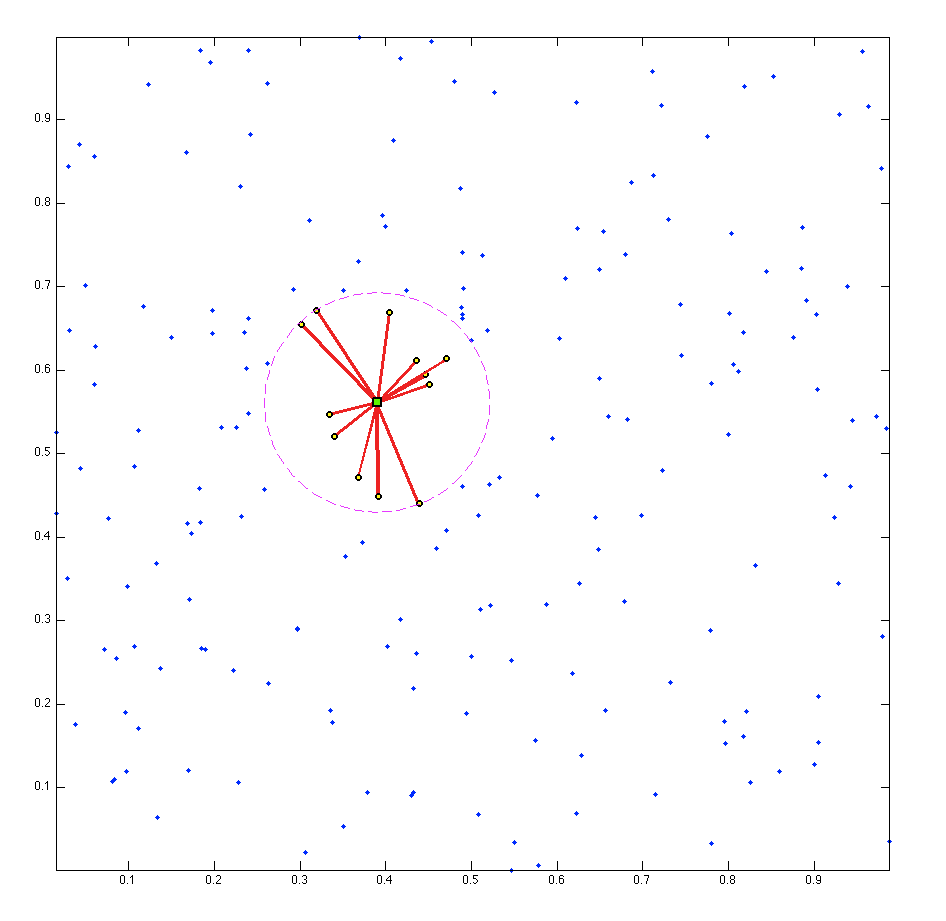
\includegraphics[width=1.0\textwidth]{../figures/chapter2/preview_stencils_example.png}
		\caption{A 13 node RBF-FD stencil of randomly distributed nodes. The stencil centered at the green square contains the 12 nearest neighbors contained within the minimum covering circle drawn in purple.}
		\label{fig:stencil_example_random}
	\end{subfigure}
	\begin{subfigure}[m]{0.35\textwidth}
		\centering
		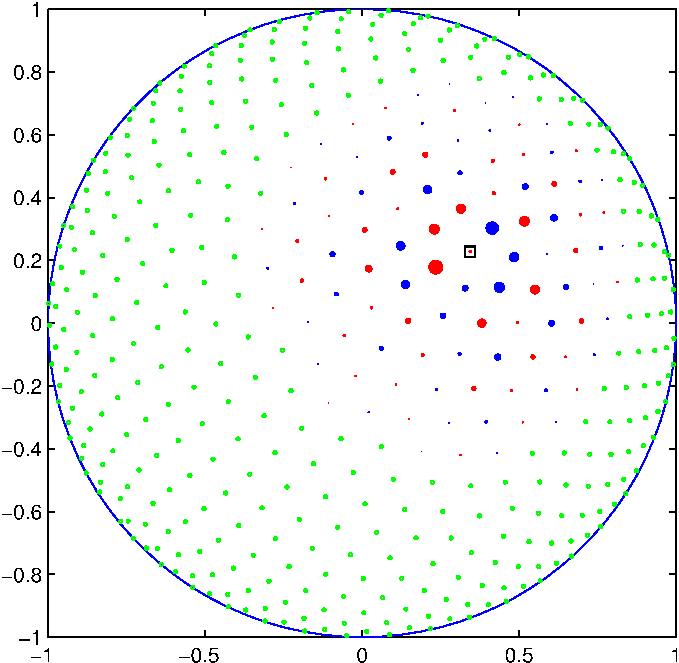
\includegraphics[width=1.0\textwidth]{../figures/chapter2/RBFFD_single-eps-converted-to.pdf}
		\caption{A 75 node RBF-FD stencil with blue (negative) and red (positive) differentiation weights to approximate advective operator at the square. Stencils weights indicated by scale of disk radii. (Image courtesy of Bengt Fornberg and Natasha Flyer)}
		\label{fig:stencil_example_sphere}
	\end{subfigure}
	\caption{Examples of stencils computable with RBF-FD}
	%TODO: Consider: show example FD stencil (5pt with regular grid)
	\label{fig:stencil_example}
\end{figure}

Figure~\ref{fig:stencil_example} provides two examples of RBF-FD stencils. First, Figure~\ref{fig:stencil_example_random} illustrates a single stencil of size $n=13$ in a domain of randomly distributed nodes. The stencil center, $x_c$, is represented by a green square, with the 12 neighboring nodes connected via red edges. The purple circle, the minimum covering circle for the stencil, demonstrates that the stencil contains only the 12 nearest neighbors of the center node. In Figure~\ref{fig:stencil_example_sphere}, a larger RBF-FD stencil of size $n=75$ on the unit sphere is shown as red and blue disks surrounding the center represented as a square. Green disks are nodes outside of the stencil. The radii and color of the red and blue disks represent the magnitude and alternating sign of coefficients, $c_j$, determined to calculate a derivative quantity at the stencil center. 

%TODO: stencil does not need to be regular distribution.
%One of the most appealing benefits of RBF-FD is its built-in support for irregular and unstructured node distributions. 





% The center node and its neighbors define a \emph{stencil}, $\{\vx\}_{i=1}^{n}$, in a localized (small) region or \emph{neighborhood} of the domain. 


%TODO: Weights for both classical Finite Difference and RBF-FD can be obtained through the solution of linear systems. In the case of Finite Difference, the system is a Vandermonde matrix. 
%TODO: For RBF-FD the system is based on a symmetric distance matrix. 
%TODO: Need better description and ref The key difference between FD and RBF-FD systems is the singularity that occurs when two nodes swap.

\subsection{Stencil Weights} 

 To approximate $\diffop{u(x)}$, one requires the stencil \emph{weights} (coefficients), ${c_j}$. Stencil weights are a discrete representation of the differential operator at the stencil center and may vary by node location (e.g., nodes at the boundary are usually governed by another operator, $\boundop$). Weights are obtained by enforcing that they be exact within the space spanned by the RBFs centered at stencil nodes (i.e., $\phi_j(x) = \phi(\epsilon ||x-x_j||_2)$; an RBF centered at $x_j$). Various studies  \cite{WrightFornberg06,FornbergDriscoll02,FornbergLehto11,FlyerLehto11} show that better accuracy is achieved when the 
interpolant can exactly reproduce a constant, $p_0$, such that	\begin{align*}
	       \left. \diffop{\phi_i(x)} \ \right|_{x=x_c} = \sum_{j=1}^{n} c_j \phi_j(x_i) + c_{n+1} p_0 \ \ \ \ \ \ \textrm{for }i=1,2,...,n  
	\end{align*}
	with $\diffop{\phi}_i$ provided by analytically applying the differential operator to the RBF. Assuming $p_0 = 1$, the constraint $\sum_{i=1}^{n}c_i=\diffop{p_0}|_{x=x_{c}}=0$ completes the system: 
	\begin{eqnarray}        
          \begin{bmatrix} \phi_1(x_1) & \phi_2(x_1) & \cdots & \phi_n(x_{1}) & 1 \\ 
            \phi_1(x_2) & \phi_2(x_2) & \cdots & \phi_n(x_{2}) & 1\\ 
            \vdots & \ddots & \ddots & \vdots & \vdots \\ 
            \phi_{1}(x_n) & \phi_{2}(x_n) & \cdots & \phi_{n}(x_{n}) & 1 
            \\ 1 & 1 & \cdots & 1 & 0 \end{bmatrix} 
            \begin{pmatrix} c_1 \\ c_2 \\ \vdots \\ c_n \\ c_{n+1} \end{pmatrix} & = & \begin{pmatrix} \left.\diffop{\phi_1}(x)\ \right|_{x=x_c} \\  \left.\diffop{\phi_2}(x)\ \right|_{x=x_c} \\ \vdots \\  \left.\diffop{\phi_{n}}(x)\ \right|_{x=x_c} \\ 0 \end{pmatrix} \label{eq:rbffd_weight_system} \\
\begin{bmatrix} \phi & P \\
		P^T & 0 \end{bmatrix} \begin{pmatrix} c_\diffop{} \\ 
							d_\diffop{} \end{pmatrix} & = & \begin{pmatrix} \phi_{\diffop{}} \\
							0 \end{pmatrix}. \nonumber
	\end{eqnarray}	
The choice of $\diffop{}$ can be any linear operator. As an example, if $\diffop$ is the identity operator, then the above procedure leads to RBF-FD weights for interpolation. If $\diffop=\pd{}{x}$, one obtains the weights to approximate the first derivative in $x$. Refer to \cite{Fasshauer2007} for a table of commonly used RBF derivatives. Section~\ref{sec:weight_operators} provides a list of derivatives used in this work. 

The small $(n + 1) \times (n + 1)$ system in Equation~\ref{eq:rbffd_weight_system} is dense, and is solved at a cost of $O(n^3)$ floating point operations (FLOPs) using direct methods like LU-decomposition. The resulting stencil weights, $c_\diffop{} = \{c_j\}_{j=1}^n$ can be substituted into Equation~\ref{eq:derivFromFDWeights} for the derivative approximation at $x_c$. Coefficient $c_{n+1}$ ($d_\diffop{} = c_{n+1}$), included in the solution of Equation~\ref{eq:rbffd_weight_system}, is of no use and discarded once the system has been solved. 

Based on the choice of support parameter, $\epsilon$, the Equation~\ref{eq:rbffd_weight_system} may suffer problems with conditioning. In such cases, stable methods like Contour--Pad\'{e} \cite{Wright2003} or RBF-QR \cite{Fornberg2011a,Davydov2011} may be preferred.  


%The above procedure 
%As an example, if $\diffop$ is the identity operator, 
%then the above procedure leads to RBF-FD interpolation. If $\diffop=\pd{}{x}$, one obtains the DM that approximates the first derivative in $x$. 

%TODO: Use of the 1's constraint is highly recommended. It keeps weights within magnitude 100, whereas not providing the constraint results in much higher magnitudes in the thousands or tens of thousands. Using first order monomials does not add benefit. Include examples of weights in 2D with 5 to 10 nodes.

%TODO: weights applied to u
\subsection{Differentiation Matrix}
Note that Equation~\ref{eq:rbffd_weight_system} resolves the weights only for the stencil $x_c$. The small system solve is repeated $N$ times---once for each stencil---to obtain a total of $N \times n$ stencil weights. 

For PDEs, it is common practice to assemble a \emph{differentiation matrix} (DM); a discrete representation of the PDE operator on the domain. Given the set of nodes in the domain $\{x_k\}_{k=1}^N$, the $c$-th row of the DM represents the discrete PDE operator for the stencil centered at node $x_c$ with stencil nodes $\{x_j\}_{j=1}^{n}$: 
\begin{align*}
 \diffop{u(x)} & \approx D_{\diffop{}} u \\
D_\diffop{}^{(c,k)} & = \begin{cases} c_j & x_k = x_j \\
                                    0 & x_k \neq x_j \\
                                    \end{cases} 
\end{align*}
where $(c,k)$ represents the (row, column) index of $D_\diffop{}$ and vector $u = \{u(x_k)\}_{k=1}^{N}$. Equation~\ref{eq:derivFromFDWeights} can be rewritten as:
\begin{align*}
\left. \diffop{u(x)} \ \right|_{x = x_c} & \approx D_{\diffop{}}^{(c)} u \ \ .
\end{align*}
In the solution of PDEs the DMs are utilized in explicit and implicit modes. Here explicit implies evaluating the matrix-vector mulitply to get derivative values, $u'$, from explicitly known vector of solution values $u$: 
\begin{align}
u' = D_{\diffop{}} u
\label{eq:explicit_eq}
\end{align}
whereas implicit solves for unknown $u$:
\begin{align}
D_{\diffop{}} u = f
\label{eq:implicit_eq}
\end{align}

An example RBF-FD DM is illustrated in Figure~\ref{fig:example_DM_rows}. In this example, assume operator $\diffop{} = \pd{}{x}$ is approximated at all $N$ stencil centers of an arbitrary domain. RBF-FD weights assemble the rows of the differentiation matrix, $D_{x}$. On each row, weights are indicated by blue dots. The sparsity of rows reflects the subset of $\{x_k\}_{k=1}^N$ included in corresponding stencils of size $n$. On the right hand side, discrete derivative values $\d{u}{x}$ are approximated at all stencil centers. 

\begin{figure}[htbp]
	\centering
		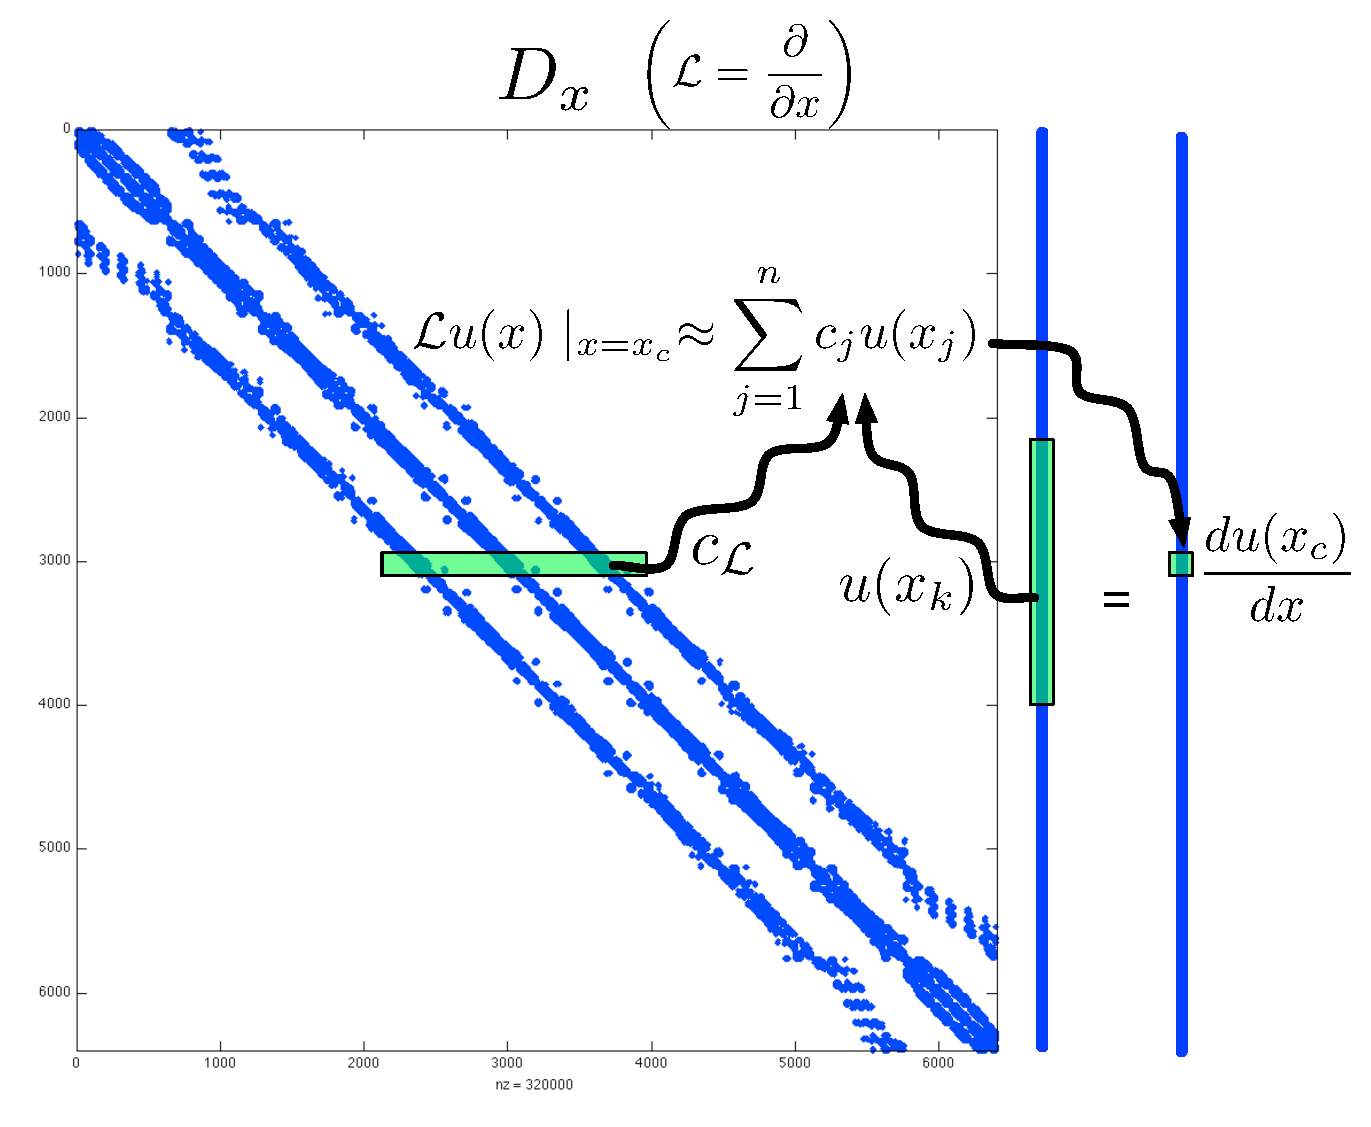
\includegraphics[width=0.65\textwidth]{omnigraffle/DM_rows.pdf}
		\caption{Differentiation matrix $D_x$ is applied to the solution values $u(x)$ to obtain derivative approximations, $\d{u}{x}$. }
		\label{fig:example_DM_rows}
\end{figure}

%TODO: note that DM does not depend on $u(x)$; only x. if the function u(x) wer
Differentiation matrices are assembled at a cost of $O(n^3 N)$ FLOPs. However, since the goal of RBF-FD is to keep stencil neighborhoods small ($n \ll N$), the cost of assembly scales as $O(N)$. Furthermore, RBF-FD weights are independent of function values ($u(x)$) and rely only on stencil node locations. The implications of this are as profound as in the context RBF-PS for time-dependent PDEs: the stencil weights are constant so long as the nodes are stationary. Thus, the DM assembly is part of a one-time preprocessing step.% and can applied explicitly in $O(N)$ operations  

%TODO: verify
% Generally speaking DM application at each time-step scales as $O(N)$ for explicit solutions and $O(N^2)$ for implicit. 

The sparsity exhibited by the DM in Figure~\ref{fig:example_DM_rows} is typical for RBF-FD due to $n \ll N$. 
%A problem of size $N$ with stencil size $n$ results in an $N \times N$ DM with only $N*n$ non-zeros. For $N=10,000$ and $n=31$, roughly $0.3\%$ of the matrix is non-zero, and the percentage only decreases as $N$ increases. 
Best practices dictate that the DMs be stored in a compressed sparse storage format to retain only non-zeros and their corresponding indices in memory. 
%TODO: This reduces the $N^2$ matrix elements to a memory footprint of  

%TODO: storage in sparse rather than dense form
%TODO: storage allows us to precompute and apply at later time-steps. 

%TODO: swapping nodes does not cause singularity



\subsection{Multiple Operators}

In many cases, multiple derivatives (e.g., $\diffop{} = \nabla^2$, $\pd{}{x}$, $\pd{}{y}$, etc.) are required at stencil centers. This is common, for example, when solving coupled PDEs. For RBF-FD, acquiring weights for each additional operator can be both straight-forward and computationally efficient. For each change of differential operator, observe that only the RHS of Equation~\ref{eq:rbffd_weight_system} is modified. Thus, new operators amount to extending Equation~\ref{eq:rbffd_weight_system} to solve 
\begin{eqnarray}
    \begin{bmatrix} \phi & P \\
		P^T & 0 \end{bmatrix} \begin{bmatrix} c_{\nabla^2} & c_{x} & c_{y} & \cdots \\ 
							d_{\nabla^2} & d_{x} & d_{y} & \dots \end{bmatrix} & = &     
		\begin{bmatrix} \phi_{\nabla^2} & \phi_{x} & \phi_{y} & \cdots \\
							0 & 0 & 0 & \cdots \end{bmatrix}. \nonumber
	\end{eqnarray}
where multiple sets of weights ($c_\nabla, c_x, c_y$) solved simultaneously. This dense, symmetric, multiple RHS linear system is considered ideal by linear algebra packages, and many highly optimized routines exist to solve them (e.g., LAPACK ``dgesv") \cite{Lapack1999}. 

%TODO: boundaries can be, but are not always handled by special operators
%TODO: preprocessing complexity vs timestep 


\subsection{Weight Operators}
\label{sec:weight_operators}
%Throughout the development of our parallel code we have verified code correctness through the solution of a variety of PDEs.
In the course of this work we work with a variety of PDEs. This section enumerates a list of relevant operators and their corresponding equations for the RHS of Equation~\ref{eq:rbffd_weight_system}. Whenever possible the general form of $\diffop{\phi}$ is provided; otherwise the Gaussian RBF ($\phi(r) = e^{-(\epsilon r)^2}$) is assumed. 

\subsubsection{First and Second Derivatives ($\frac{1}{r}\pd{\phi}{r}, \pdd{\phi}{r}$)}
The following are used in subsequent derviatives:
\begin{align*}
\frac{1}{r}\d{}{r}\phi(r) & = -2 \epsilon^2 \phi(r) \\
\pdd{\phi}{r} & = \epsilon^2(-2 + 4(\epsilon r)^2)\phi(r)
\end{align*}



\subsubsection{Cartesian Gradient ($\grad$)}
The first derivatives in Cartesian coordinates ($\pd{}{x}, \pd{}{y}, \pd{}{z}$) are produced via the chain rule:
	\begin{align*} 
	 \pd{\phi}{x} = \pd{r}{x} \pd{\phi}{r} = \frac{(x-x_{j})}{r} \pd{\phi}{r} \\
	 \pd{\phi}{y} = \pd{r}{y} \pd{\phi}{r} = \frac{(y-y_{j})}{r} \pd{\phi}{r} \\
	 \pd{\phi}{z} = \pd{r}{z} \pd{\phi}{r} = \frac{(z-z_{j})}{r} \pd{\phi}{r}
	\end{align*}
where $\pd{\phi}{r}$ for the Gaussian RBFs is given above. 


\subsubsection{Cartesian Laplacian ($\Laplacian$)}
Fasshauer \cite{Fasshauer2007} provides the general form of $\nabla^2$ in 2D as: 
\begin{align*}
\nabla^2 = \pdd{}{r}\phi(r) + \frac{1}{r}\pd{}{r} \phi(r) 
\end{align*}
For Gaussian RBFs in particular we have the following operators:
\begin{itemize}
\item 1D: $$\nabla^2 = \epsilon^2 (-2 + 4 (\epsilon r)^2) \phi(r)$$
\item 2D: $$\nabla^2 = \epsilon^2 (-4 + 4 (\epsilon r)^2) \phi(r)$$
% e^{-(\epsilon r)^2}$
\item 3D: $$\nabla^2 = \epsilon^2 (-6 + 4 (\epsilon r)^2) \phi(r)$$
% e^{-(\epsilon r)^2}$
\end{itemize}
which all fit $\nabla^2 = \pdd{}{r}\phi(r) + \frac{d - 1}{r}\pd{}{r} \phi(r)$ for dimension $d$.

%
%
%
%2D: \begin{align}
% \nabla^2 = 
% \end{align}
%3D: 
%\begin{align} 
%\epsilon^2 \\
%r^2 \\
%r^2 (\epsilon r)^2 \\
%\nabla^2 = \pd{}{x^2} = 2 \epsilon^2 ( -1 + 2 r^2 ( \epsilon r)^2) \phi(r)
%\end{align}
%
%
%\begin{verbatim}
%                eps2 = ep.^2;
%                xdv = nodes(imat,1) - nodes(imat(1),1);
%                x2eps2 = xdv.^2 * eps2;
%                switch dim
%                    case 1
%                        B(1:n, windx) = 2 .* eps2 .* (-1 + 2.*x2eps2) .* rbf.phi(ep, rdv);
%                    case 2
%                        % Imat is stencil indices
%                        % imat(1) gets stencil center
%                        % ydv = x_i.y - x_j.y
%                        % nodes(imat(1),:) = x_j
%                        ydv = nodes(imat,2) - nodes(imat(1),2);
%                        y2eps2 = ydv.^2 * eps2;
%                        B(1:n, windx) = 4 .* eps2 .* (-1 + x2eps2 + y2eps2) .* rbf.phi(ep, rdv);
%                    case 3
%                        ydv = nodes(imat,2) - nodes(imat(1),2);
%                        zdv = nodes(imat,3) - nodes(imat(1),3);
%                        r2eps4 = (xdv.^2 + ydv.^2 + zdv.^2) * eps2 * eps2;
%                        % r2eps4 = r^2 \epsilon^4
%                        B(1:n, windx) = (-6 .* eps2 + 4 .* r2eps4) .* rbf.phi(ep, rdv);
%\end{verbatim}


\subsubsection{Laplace-Beltrami ($\LaplaceBeltrami$) on the Sphere}

The $\Laplacian$ operator can be represented in spherical polar coordinates for $\mathbb{R}^3$ as: 
\begin{align*} 
\Laplacian = \underbrace{\frac{1}{r} \pd{}{r} \left( r^{2} \pd{}{r}  \right)}_{\mathsf{radial}} + \underbrace{\frac{1}{r^2} \Delta_{S}}_{\mathsf{angular}} , \label{eq:laplacian_in_spherical}
\end{align*}
where $\LaplaceBeltrami$ is the Laplace-Beltrami operator---i.e., the Laplacian operator constrained to the surface of the sphere. This form nicely illustrates the separation of components into radial and angular terms. 

In the case of PDEs solved on the unit sphere, there is no radial term, so we have:
\begin{align}
\Laplacian  \equiv \LaplaceBeltrami.
\end{align}
Although this originated in the spherical coordinate system, \cite{WrightFlyerYuen10} introduced the following Laplace-Beltrami operator for the surface of the sphere: 
\begin{align*} 
\LaplaceBeltrami = \frac{1}{4} \left[ \left(4-r^2\right) \pdd{\phi}{r} + \frac{4-3r^2}{r} \pd{\phi}{r} \right],
\end{align*} 
where $r$ is the Euclidean distance between nodes of an RBF-FD stencil and is independent of our choice of coordinate system. 

\subsubsection{Constrained Gradient ($P_{x} \cdot \grad$) on the Sphere}

Following \cite{FlyerWright09, FlyerLehto11}, the gradient operator can be constrained to the sphere with this projection matrix: 
%\frac{1}{||\mathbf{x}||}
\begin{align}
P = I - \mathbf{x} \mathbf{x}^T =  \begin{pmatrix} 
(1-x_1^2) & -x_1 x_2 & -x_1 x_3 \\
-x_1 x_2 & (1-x_2^2) & -x_2 x_3 \\ 
-x_1 x_3 & -x_2 x_3 & (1-x_3^2) 
\end{pmatrix} = \begin{pmatrix} P_{x_1} \\ P_{x_2} \\ P_{x_3} \end{pmatrix}
\label{eq:project_gradient}
\end{align}
where $\mathbf{x}$ is the unit normal at the stencil center. 


The direct method of computing RBF-FD weights for the projected gradient for $\mathbf{P} \cdot \nabla $ is presented in \cite{FlyerWright09}. When solving for the weights, we apply the projection on the right hand side of our small linear system. We let $\vx = \begin{pmatrix} x_1, x_2, x_3 \end{pmatrix} $ be the stencil center, and $\vx_k=\begin{pmatrix} x_{1,k}, x_{2,k}, x_{3,k}\end{pmatrix}$ indicate an RBF-FD stencil node. 

Using the chain rule, and assumption that 
$$r(\vx_k-\vx)=\vectornorm{\vx_k-\vx} = \sqrt{(x_{1,k}-x_1)^2 + (x_{2,k}-x_2)^2 + (x_{3,k}-x_3)^2},$$
 we obtain the unprojected gradient of $\phi$ as
\begin{align*}
\nabla \phi(r(\vx_k - \vx)) = \pd{r}{\vx} \pd{\phi(r(\vx_k - \vx))}{r} = - (\vx_k - \vx)\frac{1}{r(\vx_k - \vx)} \pd{\phi(r(\vx_k - \vx))}{r} .
\end{align*} 

Applying the projection matrix gives 
\begin{align*}
\mathbf{P} \nabla \phi(r(\vx_k - \vx)) & = - (\mathbf{P} \cdot \vx_k - \mathbf{P}\cdot\vx)\frac{1}{r(\vx_k - \vx)} \pd{\phi(r(\vx_k - \vx))}{r} \\
& =  - (\mathbf{P}\cdot\vx_k - 0)\frac{1}{r(\vx_k - \vx)} \pd{\phi(r(\vx_k - \vx))}{r} \\
& = - (I-\vx\vx^T)(\vx_k
)\frac{1}{r(\vx_k - \vx)} \pd{\phi(r(\vx_k - \vx))}{r} \\
& = \begin{pmatrix} x \vx^T \vx_k - x_k \\ y \vx^T \vx_k -  y_k \\ z \vx^T \vx_k -z_k \end{pmatrix} \frac{1}{r(\vx_k - \vx)} \pd{\phi(r(\vx_k - \vx))}{r} 
 \end{align*}
Thus, we directly compute the weights for $P_{x}\cdot\grad{}$ using these three RHS in Equation~\ref{eq:rbffd_weight_system}: 
\begin{align*} 
P\pd{}{x_1} = ( x_1 \vx^T \vx_k - x_{1,k}) \frac{1}{r(\vx_k - \vx)} \pd{\phi(r(\vx_k - \vx))}{r} |_{\vx=\vx_j} \\
P\pd{}{x_2} = ( x_2 \vx^T \vx_k - x_{2,k}) \frac{1}{r(\vx_k - \vx)} \pd{\phi(r(\vx_k - \vx))}{r} |_{\vx=\vx_j} \\
P\pd{}{x_3} = ( x_3 \vx^T \vx_k - x_{3,k}) \frac{1}{r(\vx_k - \vx)} \pd{\phi(r(\vx_k - \vx))}{r} |_{\vx=\vx_j}
\end{align*}

%TODO: finish appendix
%Alternatively, assuming weights for operators $\grad = \pd{}{x_{1}}, \pd{}{x_{2}}, \pd{}{x_{3}}$ are already computed, the projected operator could be constructed via weighting the unprojected gradient components. For example: 

%\authnote{Show accuracy of derivative approximation when using projected operator vs linear combinations of dx,dy,dz operators}


\subsubsection{Hyperviscosity $\Delta^k$ for Stabilization}

When explicitly solving hyperbolic equations, differentiation matrices encode convective operators of the form 
\begin{equation}
D = \alpha \pd{}{\lambda} + \beta \pd{}{\theta} \label{eqconv}
\end{equation}
%TODO: where $\alpha$ and $\beta$ are a function of the fluid velocity. 
The convective operator, discretized
through RBF-FD, has eigenvalues  
 in the right half-plane causing the method to be unstable~\cite{FornbergLehto11, FlyerLehto11}.  
Stabilization of the RBF-FD method is achieved through the application of a hyperviscosity filter 
to Equation~(\ref{eqconv}) \cite{FornbergLehto11}. By using Gaussian 
 RBFs, $\phi(r) = e^{-(\epsilon r)^2}$, the hyperviscosity (a high order Laplacian operator) simplifies to
\begin{equation}
\Delta^{k}\phi(r) = \epsilon^{2k} p_k(r) \phi(r)
\label{eqn:gaussian_hv}
\end{equation}
where $k$ is the order of the Laplacian and  $p_k(r)$ are multiples of generalized Laguerre polynomials that
are generated recursively (\cite{FornbergLehto11}):
\begin{align*}
\begin{cases} 
p_0(r) &=1, \\
p_1(r) &= 4(\epsilon r)^2 - 2d, \\
p_k(r) &= 4((\epsilon r)^2 - 2(k-1) - \frac{d}{2})  p_{k-1}(r) - 8(k-1)(2(k-1) - 2 + d) p_{k-2}(r), \ \ \ \ k = 2, 3, ...
\end{cases}
\end{align*}
where $d$ is the dimension of the problem. The application of hyperviscosity in Chapter~\ref{chap:explicit_implicit_pdes}, utilizes the operator as a filter to shift eigenvalues and stabilize advection equations on the surface of the unit sphere. In that case, $d=2$ is assumed ksince individual RBF-FD stencils can be viewed as (nearly) lying on a plane. For small $N$, the diameter of the stencil may not be sufficiently 
small compared to the radius of the sphere, and hyperviscosity might not work as advertised. 
%However,
%numerical evidence in \cite{FornbergLehto11,BolligFlyer} \ci suggests that if the RBFs adequately resolve the convective operator, the 2D 
%hyperviscosity operator does its job. 
%We base our work on the work of Fornberg and Lehto \cite{FornbergLehto11}, which was
%performed on a sphere, and tune our parameters following their guidelines. 

In the case of parabolic and hyperbolic PDEs, hyperviscosity is added as a filter to the right hand side of the evaluation. For example, at the continuous level, 
the equation solved takes the form
\begin{equation}
\pd{u}{t} = - \diffop u + H u,
\label{eq:evaluation_with_hyperviscosity}
\end{equation}
where $\diffop$ is the PDE operator, and $H$ is the hyperviscosity filter operator.
Applying hyperviscosity shifts all the eigenvalues of $L$ (the discrete form of $\diffop{}$) to the left half of the complex plane. 
This shift is controlled by $k$, the order of the Laplacian, and a scaling parameter $\gamma_c$, defined by
\begin{equation*}	
H = \gamma \Delta^{k} = \gamma_c N^{-k} \Delta^{k}.
\end{equation*}
It was found in \cite{FlyerLehto11}, and verified in our own application, that $\gamma = \gamma_c N^{-k}$  provides stability and good accuracy for all values of $N$ considered here. It also ensures that the viscosity vanishes as $N\rightarrow\infty$ \cite{FlyerLehto11}.
In general, the larger the stencil size, the higher the order of the Laplacian.  This is attributed to the fact that, for convective operators, larger stencils treat a wider range of modes accurately. As a result, the hyperviscosity operator should preserve as much of that range as possible. The parameter $\gamma_c$ must also be chosen with care and its sign depends on $k$ (for $k$ even, $\gamma_c$ will be negative and for $k$ odd, it will be positive). If $\gamma_c$ is too large, the eigenvalues move outside the stability domain of our time-stepping scheme and/or eigenvalues corresponding to lower physical modes are not left intact, reducing the accuracy of our approximation. If $\gamma_c$ is too small, eigenvalues remain in the right half-plane \cite{FornbergLehto11,FlyerLehto11}.


%TODO: sparsity
%TODO: Node ordering
%TODO: show blocks for boundary conditions (annulus)
%TODO: application (explicit/implicit solution)

\section{Implementation}

This section provides an overview of how one implements RBF-FD. Consider Algorithm~\ref{alg:rbffd_high_level}. The algorithm is partitioned into two phases: preprocessing and application. The complexity of each phase depends on the choice of algorithms/method utilized for each task. 

Preprocessing encompasses tasks such as grid setup/generation, stencil generation and stencil weight calculations. As output from these tasks one expects one or more DMs representing the discrete differential operators. Assuming the grid nodes do not move, the DMs remain constant for the duration of the second phase. Additionally, DMs can be loaded from disk on subsequent runs to effectively bypass the cost of all preprocessing. 


\begin{algorithm}                      
\caption{A High-Level View of RBF-FD}          
\label{alg:rbffd_high_level}                           
\textbf{Preprocessing:}
\begin{algorithmic}[0]                   
    \State $\{x\}_{j=1}^N$ = GenerateGrid()
   	\For {$j = 1$ to $N$} \label{alg:stencil_gen} 
   	    \State Stencil $\{S_{j,i}\}_{i=1}^{n}$ = QueryNeighbors($x_j$)
   	\EndFor
    \For {$j = 1$ to $N$} \label{alg:weight_calc} 
   	    \State $\{w_{j,i}\}_{i=1}^{n} = $ SolveForWeights($\{S_j\}$)
   	    \State $D_{\diffop{}}^{(j)} = $ AssembleDM($\{w_j\}$)     
    \EndFor
    \algstore{myalg}    % Store the algorithm number count
\end{algorithmic}
\textbf{Application:}
\begin{algorithmic}[1] 
\algrestore{myalg}      % continue to count from store line
    \State $t = t_{min}$                
    \While{ $t < t_{max}$ }
        \State $\{u'\} =$ SolvePDE($D_{\diffop{}}$, $\{u\}$)
        \State $\{u\} =$ UpdateSolution($\{u\}$, $\{u'\}$, $\Delta t$)
        \State $t$ += $\Delta t$
    \EndWhile
\end{algorithmic}
\end{algorithm}


The constructed DMs are applied in the Application phase to solve a PDE either explicitly or implicitly. Note that regardless of the explicit or implicit method, this phase reduces to a Sparse Matrix-Vector Multiply (SpMV) within the SolvePDE step. For explicit solutions, SolvePDE computes the SpMV in Equation~\ref{eq:explicit_eq}. In the implicit case, SolvePDE must invert the DM in Equation~\ref{eq:implicit_eq} via a direct or iterative linear system solve. Although it is not mandatory, many PDE solutions are time-dependent and require some time advancement scheme. The time-scheme could be as simple as an Euler update with a single call to SolvePDE. Higher order methods (e.g., Runge-Kutta, Adams-Bashforth, etc.) may require multiple applications of the DM, with the outputs weighted and combined within UpdateSolution. 

Tuning the performance of the RBF-FD method requires one to focus on the Application phase. This is especially true for time-dependent PDEs where an increase in grid size results in proportional increase in the number time-steps. The recurring cost of computing an SpMV each time-step quickly amortizes the one-time cost of preprocessing. 
 
On the other hand, preprocessing tasks have more impact on accuracy, stability and conditioning of the method. As each of these properties improve, the overall time to solution can decrease thanks to larger stable time-steps, smaller grid size, and fewer iterations in iterative linear system solves.

Here we discuss various design decisions in implementing the preprocessing tasks for RBF-FD and consider potential impacts on performance (if any).  Chapter~\ref{chap:rbffd_multi_gpu} will discuss Application and SpMV performance in more detail. 

\subsection{Grid} 

An implementation of RBF-FD begins with the grid. The method has no requirement for structured grids, or for a well-refined mesh/lattice that limits connectivity between nodes. It operates both on structured grids and random point clouds; although, the choice of grid does impact the accuracy of the method. This freedom to function on domains of any shape, dimension, and granularity is a major selling point for RBF-FD and often impossible for many other PDE methods. 
%Typically, the only constraint placed on the grid is that nodes should not coincide. If two nodes do coincide it is possible for a stencil to include both, and 

%TODO: cubed, ying-yang
% For example classic Finite Difference and many Finite Volume methods operate on regular/Cartesian grids. When operating on the sphere, it is common to encounter Cubed-spheres \cite{TODO:NairJablonowski08} and/or Ying-Yang grids in attempts to bypass the need for small time-steps and to alleviate troubling pole singularities common to Latitude/Longitude grids \cite{TODO}. Generalizations to unstructured meshes 
% TODO: Discontinuous Galerkin? How deep do I want to go?
%are possible for many methods (e.g., Finite Volume on multi-resolution \cite{RinglerJuGunzberger2008}) and Finite Element methods \cite{TODO}, but such methods still have a strong dependence on a Delaunay Triangulation or other mesh to determine the connectivity between nodes. 

The choice of grid is only relevant to the extent that it impacts the connectivity between nodes in stencils. Connectivity translates to non-zeros in rows of the DMs, so the various grid distributions result in a number of sparsity patterns. For all other intents and purposes, the choice of grid is only pertinent to ensure consistency with the PDEs to solve. 

In the course of this work, we applied RBF-FD to a number of PDEs and grid distributions. Here we focus on the subset utilized in Chapter~\ref{chap:explicit_implicit_pdes}. This subset is chosen for two reasons: a) to verify our solutions against existing methods, and b) easily construct refinements in 2D/3D for consistent benchmarking and convergence studies. 

%In Chapter~\ref{chap:explicit_implicit_pdes} we test the performance of our method with application to transient and steady-state PDEs. For the purpose of verification we demonstrate convergence for sets of grids previously published in the RBF literature. We briefly describe each type of grid and when it is used. 

\subsubsection{Regular Grid}
For basic debugging and benchmarking purposes the most natural choice is to start with a regular or Cartesian grid. Equally spaced nodes in multiple dimensions are simple to generate. Additionally, refinements---for convergence tests---are direct subsamples. 

In theory, RBF-FD functions the same whether nodes are uniformly spaced or random. However, regular grids do not fully exercise advantages that RBF-FD has over other methods with its ability to operate on scattered nodes.


\subsubsection{Maximum Determinant Nodes}

In Chapter~\ref{chap:explicit_implicit_pdes} we verify our RBF-FD implementation by solving PDEs on the unit sphere. For consistency in verification, we choose the Maximum Determinant (MD) node sets \cite{Sloan2001, Sloan2003} to compare against related investigations (e.g., \cite{Fornberg2009a, Fornberg2007,FornbergLehto11}). %TODO: need ref Sloan2001

As \cite{FornbergLehto11} explain choice to use MD nodes in references such as \cite{FornbergLehto11,Fornberg2009a} is based on numerical stability exhibited spherical harmonics interpolation on the node sets. 

MD node sets have gained popularity in the RBF community due demonstrated success in spherical harmonics interpolation, where the seemingly irregular distribution of nodes is demonstrated to achieve  
The node sets are available for download on the authors' web site (\url{http://web.maths.unsw.edu.au/~rsw/Sphere}), and range in size from $N=4$ up to $N=27556$. 


In case of interpolation with spherical harmonics, the MD node sets are much more stable numerically
than the ME (minimal energy) type sets [29]. This is due to the MD nodes’ subtle location irregularities, which can be seen in
Fig. 4.1. This difference in stability is therefore also present for global RBFs in their e?0 limit [14], but it becomes insignificant
for larger e-values. Tests that we have carried out show that such node location details are irrelevant also for the accuracy
and robustness of the RBF-FD approach.

Two sets of MD nodes are plotted in Figure~\ref{fig:md_nodes}. On the left is $N=4096$ and the right $N=8100$. 

Node sets from 1024 to 27,556 are considered with stencil sizes ranging from
17 to 101.
\begin{figure} 
\centering
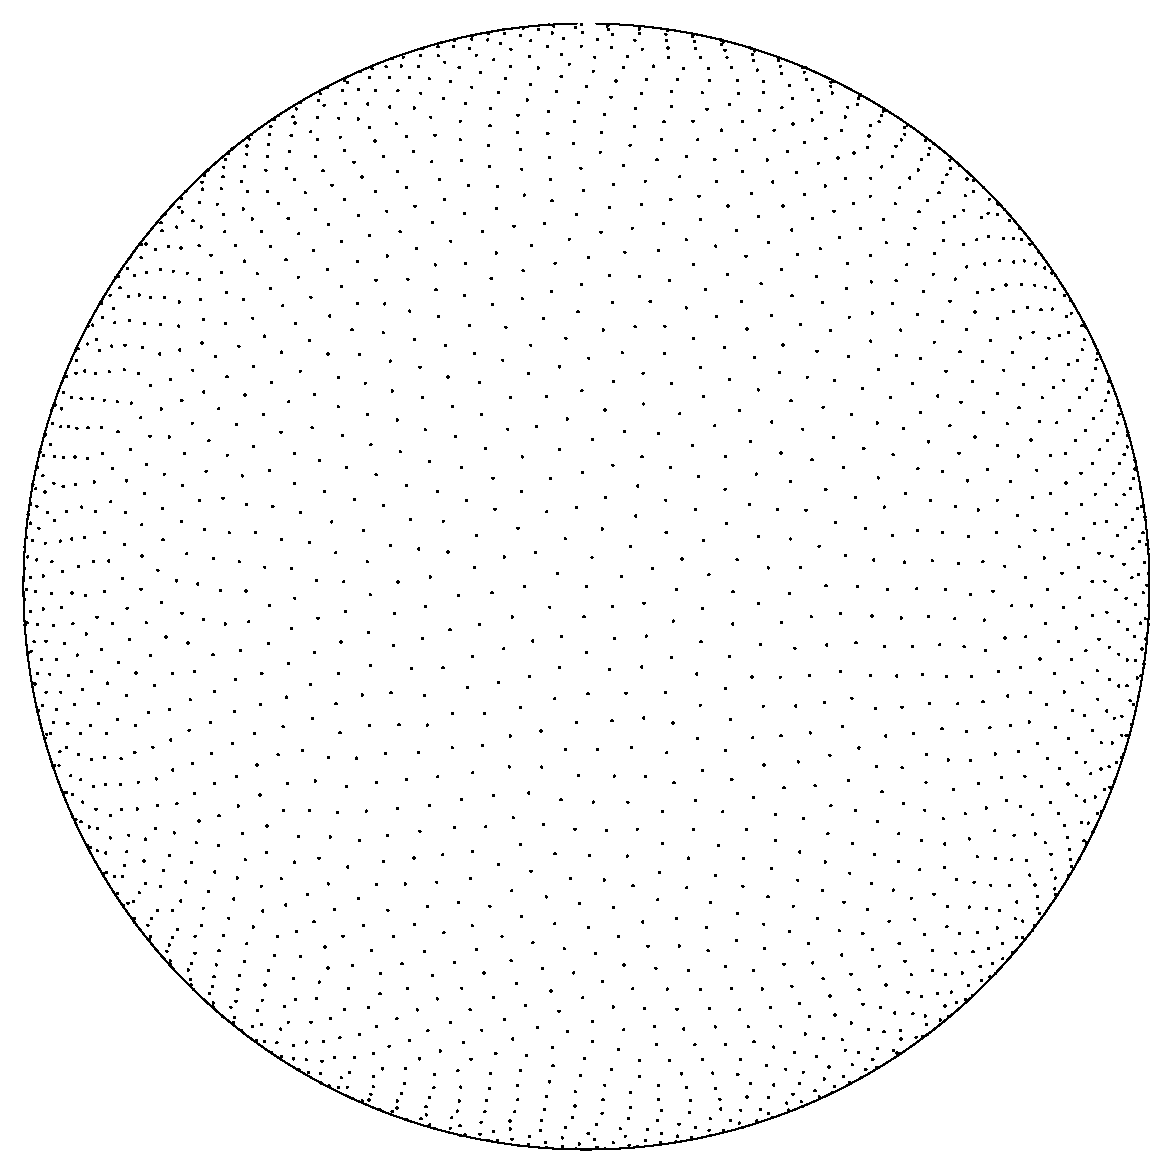
\includegraphics[width=0.4\textwidth]{rbffd_methods_content/grids/N4096_points.pdf} 
\caption{Example of $N=4096$ maximum determinant (MD) node sets on the unit sphere.} 
\label{fig:md_nodes}
\end{figure}



\begin{itemize}
\item Benefits: well studied refinements; many applications in RBF literature
\item Pitfalls: limited resolution ($27556$ max); 
\end{itemize}


\subsubsection{Centroidal Voronoi Tessellations}
To test scaling of our implementations problems greater than $N=27,556$ are required. To this end we leverage Centroidal Voronoi Tessellations (CVTs) of the sphere for higher resolution grids. 
For large node sets we also consider CVTs since they keep nodes from overlapping. 
Have I mentioned nodes should not coincide with RBF-FD? 
CVT simple algorithm (Lloyd’s)

\begin{itemize}
\item Benefits: theoretically unbounded resolution; converged grids have a sense of ``optimal" node placement; 
\item Pitfalls: refinements are not direct; long time to convergence; limited to 1M nodes
\end{itemize}

% TODO: mention other grids generated with CVTs and provide examples 
\subsubsection{Other Grids}

% TODO: wanted to test without the presence of boundary conditions 
% TODO: other grids tested boundary conditions

Integrating CVTs within our implementation opens the door to a plethora of applications. While not discussed in detail in the following sections, CVTs were used to generate other complex geometries such as the 3D sphere shell, 2D annulus, ellipse and ellipsoid, 

Other grids considered during the thesis, but not included in the applications below: 

\begin{itemize}
\item Anulus
\item Nested Sphere CVT
\item a
\end{itemize}


\subsection{On Choosing the Right $\epsilon$} 
% TODO: expand missing content

%First, the method is not infallible; it faces similar conditioning issues as global/compact RBF method in that the success of the method depends on the choice of support parameter, $\epsilon$. Second, proper choice of $\epsilon$ varies based on the underlying node distribution, as well as the generated stencils. Third, the complexity of the method is low, but there are a few 

If solving for the weights directly (i.e., inverting Equation~\ref{eq:rbffd_weight_system}), one must carefully choose $\epsilon$ to prevent ill-conditioning. Numerous attempts exist in literature to provide ``good" functions for $\epsilon$ based on node spacing, $h$, stencil size $n$, etc. In general, the values provided are particular to the specific problem and/or grid under consideration. No fool-proof method exists to select the support parameters, so the prospect of hassle-free application of the RBF-FD method is still out of reach. 

Modern algorithms introduced in the last couple years provide methods for acquiring weights. Contour-Pad\'{e}, RBF-QR, and RBF-GA are all options for weights corresponding to the $\epsilon \rightarrow 0$. These methods appear to resolve many issues including conditioning of implicit systems for more accurate solutions \cite{Davydov2011}  \cite{Fornberg2013} 

In this work, we have attempted a variety of scalings on $\epsilon$. We forego discussion of these attempts since they are outside our current scope of investigation. In the end, we find that the most effective method for choosing $\epsilon$ was to adopt the approach introduced in \cite{FlyerLehto11}, wherein $\epsilon$ is expressed as a function of the number of nodes $N$ and desired mean condition number, $\bar{\kappa}_A$. 

%TODO: what papers provide epsilon choice? based on grid? based on node density? proportional to what?
%TODO: what is the algorithm to choose epsilon?
%TODO: what examples are provided? 
%TODO: does the choice of c1 and c2 depend on the problem? 
%TODO: what level coarse grid is necessary to get contours? 
%TODO: what other epsilon tests? why not uniform epsilon? why not variable epsilon? 

%TODO: add references and descriptions. 
The optimal $\epsilon$ for general node distributions is out of the scope of this research and not necessary for our purposes. For now we assume that nodes are more or less regularly distributed, either via some algorithm such as Lloyd's method to create Centroidal Voronoi Tessellations, repelling springs (distmesh), minimum energy or minimum determinant, or some other algorithm. Except in cases where convergence on PDE solutions can not be attained via RBF-FD, we find that a direct solve for RBF-FD weights is sufficient. To a certain extent, this work considers parallelization of the method so it does not matter if our weights are precise or not. 

\subsection{Generating Stencils}
%reply to the LSH question from the reviewer involving parallelization of the search process for each point, and the issue regarding embarrassingly parallel process. Also note: this is done only once so efficiency is not an issue, nor is parallelization.

For each of the $N$ small system solves of Equation~(\ref{eq:rbffd_weight_system}), the $n$ nearest neighbors to $\vx_j$ need to be located. This can be done efficiently using neighbor query algorithms or spatial partitioning data-structures such as Locality Sensitive Hashing (LSH) and $k$D-Tree. Different query algorithms often have a profound impact on the DM structure and memory access patterns. We choose a Raster ($ijk$) ordering LSH algorithm \cite{Bollig2011} leading to the matrix structure in Figures~\ref{fig:oneThreadPerStencil} and \ref{fig:oneWarpPerStencil}. While querying neighbors for each stencil is an embarrassingly parallel operation, the node sets used here are stationary and require stencil generation only once. Efficiency and parallelism for this task has little impact on the overall run-time of tests, which is dominated by the time-stepping. We preprocess node sets and generate stencils serially, then load stencils and nodes from disk at run-time. In contrast to the RBF-FD view of a static grid, Lagrangian/particle based PDE algorithms promote efficient parallel variants of LSH in order to accelerate querying neighbors at each time-step \cite{Pan2011, Goswami2010}. 


Many algorithms exist to query the $k$-nearest neighbors (equivalently all nodes in the minimum/smallest enclosing circle). Some algorithms overlay a grid similar to Locality Sensitive Hashing and query such as... \cite{HarPeledMazumdar2003}.

RBF-FD is designed to handle irregular node distributions. Therefore, it is not essential that stencils contain only nearest neighbors. Instead, one can acquire the \emph{approximate nearest neighbors}. Figure~\ref{fig:ann_example} demonstrates a case where a does not contain all nearest neighbors. As illustrated in the Figure, the ANN stencil and true nearest neighbor stencil differ by one node. THis is not dire


\subsubsection{KDTree}

\subsubsection{Hashing}

Hashing, shown in Figure~\ref{fig:hashing_example} overlays a regular grid. This is equivalent to an axis aligned bounding box AABB, with refinement. In other words, we form a quad-tree in 2D, an octree in 3D. The neighbor query starts with the cell in which $x_c$ resides. Since we use an axis aligned bounding box, this cell index is easily calculated given the coordinate and number of subdivisions in each dimension. Once the cell index is resolved, the stencil is populated by taking the $n$ nearest neighbors from within the current cell. If the cell does not contain sufficient number of nodes to fill the stencil, the search for neighbors expands to include the cells immediately adjoining the center cell, taking only the nearest nodes in the provided cells. The search continues to expand outward in a rasterized circle/sphere until $n$ is satisifed. This search is considered approximate because it can happen that a true nearest neighbor would lie in a cell that is is not included in the rasterized circle, and other nodes are substituted from the far reaches of the discretized grid.

%TODO: cite lagrangian sph knn
The complexity of the method is still higher than the more efficient implementations used by Lagrangian methods, but as demonstrated in Figure~\ref{sten_methods_compare} the savings are significant. Generating stencils for RBF-FD is a preprocessing cost, so we do not dedicate an excessive amount of attention to this algorithm. However, a few ideas that would improve: hilbert ordering, choose AABB resolution based on $N$ not user parameters, faster sorting, GPU implementation


\subsubsection{Savings}
To demonstrate the savings in choice of stencil generation method, we provide Figure~\ref{fig:sten_methods_compare}. 





\subsection{Node Placement -- Centroidal Voronoi Tessellation}



We make the assumption for now that we use regularly distributed nodes. Centroidal Voronoi tessellations provide reasonably good distributions for solutions. Examples (heat ellipse, ellipsoid, sphere, square cavity).

The motivation behind RBF-FD is generality/functionality in the numerical method. Scattered nodes are supported. Distribution requires proper choice of support, and tight nodes result in increased conditioning

\subsection{Approximate Nearest Neighbor (ANN) Query}

RBF-FD operates on general node distributions. Historically, stencils are uniform in size ($n$) and generated by selecting the $(n-1)$ true nearest neighbors to a node $x_c$. This is a $k$-NN query. 

Alternative queries are possible: ball query and approximate nearest neighbor. The approximate is of particular interest because nodes closest to the stencil will always be selected, whereas the nodes further away have minimal influence so swapping out cant hurt. The justification in altering the selection is for reduced complexity in neighbor queries.  

%RBF methods are traditionally described as general and meshless in that they apply to unstructured clouds of points in arbitrary dimensions. However, although the term meshless implies a method capable of operating with no node connectivity, all numerical methods---meshless RBF methods included---connect nodes in the domain. For example, the ``meshless'' global RBF method connects every node in the domain to all other nodes. Compact support or local RBF methods like RBF-FD limit connections to nodes that lie within a predetermined radius.

%The connections between nodes form a directed adjacency graph with edges that dictate the paths along which data/phenomena can travel. For example, a plus shaped stencil of five points with a center node and four neighboring nodes allows values to propagate north, south, east and west; not northeast, southeast, etc.


%They are robust and function on scattered point clouds. RBF-FD in particular requires stencils to be generated from $n$ nearest neighbors to a stencil center. The cost of these neighbor queries can vary greatly depending on the choice of algorithm or data-structure used to make the query. 

For example, in general brute force is inefficient 
The author of \cite{Fasshauer2007} queries $n$ nearest neighbors for a compact-support RBF partition of unity example with a $k$-D tree. In \cite{FlyerLehto11,FornbergLehto11} a $k$-D Tree is leveraged for all neighbor queries for RBF-FD. 

In our work in \cite{BolligFlyerErlebacher2012} an alternative to $k$-D tree was leveraged, based loosely on Locality Sensitive Hashing. 

Rather than iterate through all $N$ nodes to find the true neighbors, or step through a k-D tree in something like $O(log N)$ that requires extra built-out, ANN allows us to use a set of nodes that satisfy

\subsubsection{$k$-D Tree}

Most of the RBF community leverages the $k$-D tree, due to its low computational complexity for querying neighbors and its wide availability as standalone software in the public domain (e.g., matlab central has a few implementations for download, and the MATLAB Statistics Toolbox includes an efficient k-D Tree). 

The complexity of assembling he tree is

The Matlab central $k$-D Tree is MEX compiled and efficient. We integrated the standalone C++ code into our library.  

While the $k$-D Tree functions well for queries, its downfall is a large cost in preprocessing to build the tree. For moving nodes, such as in Lagrangian schemes, this cost is prohibitively high. In an attempt to reduce the cost, lagrangian schemes introduced approximate nearest neighbor queries based on 

Approximate nearest neighbors will be nearly balanced. 
We observe that RBF-FD functions as well on stencils of true nearest neighbors as it does on approximate nearest neighbors. 


\subsubsection{Sparsity}
To quantify the sparsity of a Differentiation Matrix we consider the ratio of non-zeros ($N*n$) to total elements in the matrix ($N^2$). For example, a problem of size $N = 10,000$ with stencil size $n=31$ has a ratio of $0.0031$ and is $99.69\%$ empty. 

%TODO: sparsity
%TODO: Node ordering
%TODO: show blocks for boundary conditions (annulus)





\chapter{A Distributed Multi-GPU RBF-FD Implementation}
\label{chap:rbffd_multi_gpu}

%\authnote{Related work for start of Parallel/GPU chapter}
Parallel implementations of RBF methods currently rely on parallel domain decomposition. Depending on the implementation, domain decomposition not only accelerates solution procedures, but can decrease the ill-conditioning that plague all global RBF methods \cite{Divo2007}. The ill-conditioning is reduced if each domain is treated as a separate RBF domain, and the boundary update is treated separately. Domain decomposition methods for RBFs were introduced by Beatson et al. \cite{Beatson2000} in the year 2000 as a way to increase problem sizes into the millions of nodes.

Divo and Kassab \cite{Divo2007} used a domain decomposition method with artificial 
subdomain boundaries for their implementation of a local collocation method \cite{Divo2007}. 
Subdomains are processed independently. The derivative values 
at artificial boundary points are averaged to maintain global consistency of physical values. Their implementation 
was designed for a 36 node cluster, but benchmarks and scalability tests are not provided.

% Divo: it seems almost unnecessary to use domain decomposition if they have the local method.
% I suppose the domain decomposition is necessary for averaging physical values more than RBF collocation.

Kosec and \v{S}arler \cite{Kosec2008} used OpenMP to parallelize coupled heat transfer 
and fluid flow problems on a single workstation. 
Their test cases used local collocation, explicit time-stepping and Neumann boundary conditions. A speedup 
factor of 1.85x over serial execution was achieved by executing on two CPU cores; no 
results from scaling tests were provided. 

Stevens et al. \cite{Stevens2009a} mention a parallel implementation under development, but no document is available yet. 

Additional RBF implementations are discussed at the end of this chapter in the context of parallel co-processing with the GPU. 

In this work, we will add to the above experiences, with the added twist of incorporating an implementation on the GPU (see later chapters). 


RBFs on GPU work: \cite{Schmidt2009a, Schmidt2009b} (global), \cite{Yokota2010} (compact)


We are investigating optimizations that target both GPUs and Phi cards for a class of numerical methods based on Radial Basis Functions (RBFs) to solve Partial Differential Equations. RBF methods are increasingly popular across disciplines due to their low complexity, natural ability to function in higher dimension with minimal requirements for an underlying mesh, and high-order---in many cases, spectral---accuracy. RBF methods can be viewed as generalizations of many traditional methods such as Finite Difference and Finite Element to allow for truly unstructured grids. This generalization allows one to reuse many of the same techniques (e.g., sparse matrices, iterative solvers, domain decompositions, etc.) to efficiently obtain solutions. The variety of hardware available on Cascade will help us establish a clear argument in the choice of accelerator type and resolve the dilemma between choosing Phi vs GPU for our method. Since RBFs generalize other methods, our results should have broad reaching impact to answer similar questions for related methods.


}

%\part{Appendices}
%\appendix
%The following appendices are included to illuminate subtleties of the RBF-FD method. The first discusses the method's ability to avoid pole singularities when applied to solid body transport on the sphere. The second considers the difference between directly computing weights for differentiation operators versus leveraging linear combinations of weights to indirectly construct the same operators. 
%%\makeatletter
%\@ifundefined{standalonetrue}{\newif\ifstandalone}{}
%\@ifundefined{section}{\standalonetrue}{\standalonefalse}
%\makeatother
%\ifstandalone
%\documentclass{report}
%
%\usepackage{textcase}
%\usepackage{hyperref}
%\hypersetup{breaklinks=true}


% Added packages
\usepackage[usenames]{color}
\usepackage{amsfonts, amsmath, amssymb, graphics}

% NOTE: bibentry MUST appear before the hyperref or build will fail
\usepackage{bibentry}
\nobibliography*
\usepackage[square,sort,comma,numbers]{natbib}
  
\usepackage{float}
\usepackage[
	hidelinks,%
    %hyperindex=true,		% Make numbers of index links as well
   	backref=page, 		% Provide page listing where refs occur in the bibliography
	%breaklinks=true,
    %colorlinks,%
    %citecolor=green,%
    %filecolor=blue,%
    %linkcolor=red,%
    %urlcolor=red, 
]{hyperref}

\usepackage{dsfont}
%%%% USEPACKAGES for MACROS %%%%%
\usepackage{algpseudocode}
\usepackage[chapter]{algorithm}
%\usepackage{caption}
\usepackage{subcaption}
\usepackage{url}

\usepackage{array}
\usepackage{arydshln}
\usepackage{multirow}
\usepackage{multicol}
%\usepackage[section]{placeins}

\input{macros/macros.tex}
\input{macros/authnote_macros.tex}
%\input{macros/track_changes_macros.tex}
\input{macros/misc_mac.tex}
\input{macros/aliases.tex}
\input{macros/table_macros.tex} 


%\usepackage{xcolor}

%\usepackage{refcheck}
% Sepia
%\definecolor{myBGcolor}{HTML}{F6F0D6}
%\definecolor{myTextcolor}{HTML}{4F452C}
% Dark
%\definecolor{myBGcolor}{HTML}{3E3535}
%\definecolor{myTextcolor}{HTML}{CFECEC}
%\color{myTextcolor}
%\pagecolor{myBGcolor}
 
%
%\begin{document}
%\fi

\chapter{Avoiding Pole Singularities with RBF-FD}
This content follows \cite{FlyerWright07,FlyerWright09}. 

Within the test cases of this dissertation, we solve convective PDEs on the unit sphere with the form: 
$$
\pd{h}{t} = \vu \cdot \nabla h
$$
where $\vu$ is velocity. For example, the cosine bell advection has this particular form:
\begin{equation}
\pd{h}{t} = \frac{u}{\cos{\theta}} \pd{h}{\lambda} + v \pd{h}{\theta} \label{eq:cosine_bell_appendix}
\end{equation}
in the spherical coordinate system defined by
\begin{align*}
x & = \cos{\theta}\cos{\lambda} \\
y & = \cos{\theta}\sin{\lambda} \\
z & = \sin{\theta}
\end{align*}
where $\theta \in (-\frac{\pi}{2}, \frac{\pi}{2})$ is the elevation angle and $\lambda \in (-\pi,\pi)$ is the azimuthal angle.
Observe that as $\theta \rightarrow \pm \frac{\pi}{2}$, the $\frac{1}{\cos{\theta}}$ term goes to infinity as a discontinuity. 

One of the many selling points for RBF-FD and other RBF methods is their ability analytically avoid pole singularities, which arise from the choice of coordinate system and not from the methods themselves. Since RBFs are inherently based on Euclidean distance between nodes, and not geodesic distance, it is said that they do not ``feel'' the effects of the geometry or recognize singularities naturally inherent in the coordinate system \cite{FlyerWright07}. 
Here we demonstrate how pole singularities are analytically avoided with RBF-FD for cosine bell advection.  


Let $r = || \vx - \vx_j ||$ be the Euclidean distance which is invariant of the coordinate system. In Cartesian coordinates, we have
$$
r = \sqrt{(x-x_j)^2 + (y-y_j)^2 + (z-z_j)^2}.
$$
In spherical coordinates we have:
$$
r = \sqrt{2(1-\cos{\theta}\cos{\theta_j}\cos{(\lambda-\lambda_j)} - \sin{\theta}\sin{\theta_j})}.
$$

The RBF-FD operators for $\d{}{\lambda}, \d{}{\theta}$ are discretized with the chain rule: 

\begin{align}
\d{\phi_{j}(r)}{\lambda} = \d{r}{\lambda} \d{\phi_{j}(r)}{r} & = \frac{\cos{\theta}\cos{\theta_j}\sin{(\lambda - \lambda_j)}}{r} \d{\phi_j(r)}{r}, \label{eq:rbfffd_d_dlambda} \\
\d{\phi_{j}(r)}{\theta} = \d{r}{\theta} \d{\phi_{j}(r)}{r} & = \frac{\sin{\theta}\cos{\theta_j}\cos{(\lambda-\lambda_j)} - \cos{\theta}\sin{\theta_j}}{r} \d{\phi}{r}, \label{eq:rbfffd_d_dtheta}
\end{align}
where $\phi_{j}(r)$ is the RBF centered at $\vx_{j}$. 

Plugging \ref{eq:rbfffd_d_dlambda} and \ref{eq:rbfffd_d_dtheta} into \ref{eq:cosine_bell_appendix}, produces the following explicit form: 
\begin{align*}
\d{h}{t} = u(\cos{\theta_j}\sin{(\lambda - \lambda_j)} \frac{1}{r} \d{\phi_j}{r}) + v (\sin{\theta}\cos{\theta_j}\cos{(\lambda-\lambda_j)} - \cos{\theta}\sin{\theta_j} \frac{1}{r} \d{\phi}{r}) 
\end{align*}
where $\cos{\theta}$ from \ref{eq:rbfffd_d_dlambda} analytically cancels with the $\frac{1}{\cos{\theta}}$ in \ref{eq:cosine_bell_appendix}.


Then, formally, one would assemble differentiation matrices containing weights for the following operators: 
\begin{align}
\D_\lambda & = \cos{\theta_j}\sin{(\lambda - \lambda_j)} \frac{1}{r} \d{\phi_j}{r}, \label{eq:dm_lambda} \\
\D_\theta &=  \sin{\theta}\cos{\theta_j}\cos{(\lambda-\lambda_j)} - \cos{\theta}\sin{\theta_j} \frac{1}{r} \d{\phi}{r}, \label{eq:dm_theta}
\end{align} 
and solve the explicit method of lines problem:
$$
\d{h}{t} = u \D_\lambda h + v \D_\theta h
$$
where now the system is completely free of singularities at the poles \cite{FlyerWright09}. 

We note that the expression $\cos{(\frac{\pi}{2})}$ evaluates on some systems to a very small number rather than zero (e.g., $6.1(10^{-17}$) on the Keeneland system with the GNU gcc compiler). The small value in turn allows $\frac{1}{\cos{\theta}}$ to evaluate to a large value (e.g., $1.6(10^{16})$) rather than ``inf" or ``NaN". A large value allows the cosine terms to cancel in double precision, whereas an ``inf'' or ``NaN'' would corrupt the numerics. Rather than avoid placing nodes at the poles, or assuming the machine will numerically cancel the singularities, it is preferred to use operators \ref{eq:dm_lambda}, \ref{eq:dm_theta} on the RHS of Equation~\ref{eq:rbffd_weight_system} to compute RBF-FD weights. 

%
%\ifstandalone
%\bibliographystyle{plain}
%\bibliography{merged_references}
%\end{document}
%\else
%\expandafter\endinput
%\fi
%%\makeatletter
%\@ifundefined{standalonetrue}{\newif\ifstandalone}{}
%\@ifundefined{section}{\standalonetrue}{\standalonefalse}
%\makeatother
%\ifstandalone
%\documentclass{report}
%
%\usepackage{textcase}
%\usepackage{hyperref}
%\hypersetup{breaklinks=true}


% Added packages
\usepackage[usenames]{color}
\usepackage{amsfonts, amsmath, amssymb, graphics}

% NOTE: bibentry MUST appear before the hyperref or build will fail
\usepackage{bibentry}
\nobibliography*
\usepackage[square,sort,comma,numbers]{natbib}
  
\usepackage{float}
\usepackage[
	hidelinks,%
    %hyperindex=true,		% Make numbers of index links as well
   	backref=page, 		% Provide page listing where refs occur in the bibliography
	%breaklinks=true,
    %colorlinks,%
    %citecolor=green,%
    %filecolor=blue,%
    %linkcolor=red,%
    %urlcolor=red, 
]{hyperref}

\usepackage{dsfont}
%%%% USEPACKAGES for MACROS %%%%%
\usepackage{algpseudocode}
\usepackage[chapter]{algorithm}
%\usepackage{caption}
\usepackage{subcaption}
\usepackage{url}

\usepackage{array}
\usepackage{arydshln}
\usepackage{multirow}
\usepackage{multicol}
%\usepackage[section]{placeins}

\input{macros/macros.tex}
\input{macros/authnote_macros.tex}
%\input{macros/track_changes_macros.tex}
\input{macros/misc_mac.tex}
\input{macros/aliases.tex}
\input{macros/table_macros.tex} 


%\usepackage{xcolor}

%\usepackage{refcheck}
% Sepia
%\definecolor{myBGcolor}{HTML}{F6F0D6}
%\definecolor{myTextcolor}{HTML}{4F452C}
% Dark
%\definecolor{myBGcolor}{HTML}{3E3535}
%\definecolor{myTextcolor}{HTML}{CFECEC}
%\color{myTextcolor}
%\pagecolor{myBGcolor}
 
%
%\begin{document}
%\fi


\chapter{Projected Weights on the Sphere} 
\label{app:indirect_weights}

Operating on the sphere requires constrained operators described in Section~\ref{sec:projected_grad}:
\begin{align}
\mathbf{P} \cdot \nabla \phi_{k}(r(\vx)) & = \mathbf{P} \cdot \frac{(\vx-\vx_{k})}{r(\vx)} \d{\phi_{k}(r(\vx))}{r(\vx)}  \nonumber \\
& = -\mathbf{P} \cdot \vx_{k}\frac{1}{r(\vx)} \d{\phi_{k}(r(\vx))}{r(\vx)}  \nonumber \\ %\label{eq:xsfc_negative}
& = \begin{pmatrix} x \vx^{T} \vx_{k} - x_{k} \\  y \vx^{T} \vx_{k} - y_{k} \\  z \vx^{T} \vx_{k} - z_{k} \end{pmatrix} \frac{1}{r(\vx)} \d{\phi(r(\vx))}{r} \label{eq:sfc_gradient_operator}.
\end{align}
where 
\begin{align}
P = I - \mathbf{x} \mathbf{x}^T =  \begin{pmatrix} 
(1-x_1^2) & -x_1 x_2 & -x_1 x_3 \\
-x_1 x_2 & (1-x_2^2) & -x_2 x_3 \\ 
-x_1 x_3 & -x_2 x_3 & (1-x_3^2) 
\end{pmatrix} 
\label{eq:sfc_project_gradient}
\end{align}
%The operator $\mathbf{I} - \vx \vx^{T}$ for $\vx = (x,y,z)$ projects a vector onto the plane tangent to the unit sphere at $(x,y,z)$. Therefore, Equation~\ref{eq:sfc_gradient_operator} gives the projection of the gradient operator at $\vx_{k}$ onto the plane tangent to $\vx$. 

Here we investigate the difference between constructing DMs using Equation~\ref{eq:sfc_gradient_operator} on the RHS of Equation~\ref{eq:rbffd_weight_system} versus composing DMs for the standard Cartesian $\grad$ operator and combined using Equation~\ref{eq:sfc_project_gradient}.


\section{Direct Weights} 

Following \cite{FlyerLehto11}, \ref{eq:sfc_gradient_operator} takes the following form when adapted to RBF-FD:  
\begin{equation}
[ \mathbf{p}_{x} \cdot \nabla{f(\vx)}] |_{\vx = \vx_{c}} = \sum_{k=1}^{n} c_{k} \underbrace{\left[ x_{c} \vx_{c}^{T} \vx_{k} - x_{k} \right] \frac{1}{r} \d{\phi(r(x_{c}))}{r}}_{B_{c,k}^{\mathbf{p}_{x}}}. 
\label{eq:xsfc_operator_flyer_et_al}
\end{equation}
and so forth for the $\mathbf{p}_{y} \cdot \nabla, \mathbf{p}_{z}  \cdot \nabla$ operators, where $\vx_{c}$ is the stencil center and $\vx_{k}$ are stencil nodes. To compute RBF-FD weights for the $\mathbf{p}_{x} \cdot \nabla$ operator, the RHS of Equation~\ref{eq:rbffd_weight_system} is filled with elements $B_{c,k}^{\mathbf{p}_{x}}$. We will refer to this method of obtaining the weights as the \emph{direct} method due to the ability to directly compute RBF-FD weights for the operators $\mathbf{P} \cdot \nabla $, and assemble the differentiation matrices $\D_{\mathbf{p_{x}} \cdot \nabla}, \D_{\mathbf{p_{y}} \cdot \nabla}, \D_{\mathbf{p_{z}} \cdot \nabla}$ without the need to compute   and/or store other weights.

\section{Indirect Weights} 

%TODO: refer to sloan2001 for a set of test functions on the sphere that would be good test cases. 

Alternatively, weights can be computed \emph{indirectly} as a weighted combination of existing RBF-FD DMs for the unprojected $\nabla$ operator. Here we assume that differentiation matrices to compute the components of $\nabla$ are readily available in memory: 
$$
\D_{\nabla} = \begin{pmatrix} \D_{x} \\ \D_{y} \\ \D_{z} \end{pmatrix},
$$
where each matrix contains weights computed with the operators from Section~\ref{sec:rbffd_grad_weights} applied to the RHS of Equation~\ref{eq:rbffd_weight_system}.  

The differentiation matrices for $\mathbf{P} \cdot \nabla$ can then be assembled as a weighted combination of the differentiation matrices for the unprojected operator: 
\begin{equation}
\D_{\mathbf{P} \cdot \nabla} = \begin{pmatrix} \D_{\mathbf{p_{x} \cdot \nabla}} \\  \D_{\mathbf{p_{y}\cdot \nabla}} \\  \D_{\mathbf{p_{z}\cdot \nabla}} \end{pmatrix} = \begin{pmatrix} 
diag(1-X^{2}) \D_{x} - diag(XY) \D_{y} - diag(XZ) \D_{z} \\
- diag(XY)\D_{x} + diag(1-Y^{2}) \D_{y} - diag(YZ) \D_{z} \\
- diag(XZ)\D_{x} - diag(YZ) \D_{y} + diag(1-Y^{2}) \D_{z} 
\end{pmatrix}
\end{equation}
 where $X = \{x_{c,i}\}_{i=1}^{N}$, $Y = \{y_{c,i}\}_{i=1}^{N}$, $Z = \{z_{c,i}\}_{i=1}^{N}$ are the individual component values of the stencil centers $\{\vx_{c,i}\}_{i=1}^{N}$ respectively (i.e., $x_c = (x_c, y_c, z_c)$). 
%TODO: Gordon discussion: B1: explain why we use this manufactured solution. what was it designed to check.

This concept equates to classical Finite Differences where for example, the standard 5-point finite difference formula in 2-D for approximating the Laplacian can be expressed a weighted combination of coefficients for 1-D differences. 

Indirectly computing weights is of interest for at least two reasons: 
\begin{itemize}
\item The potential for memory conservation. For example, consider a coupled PDE that requires four operators: $D_x, D_y, D_z, D_{\Laplacian{}}$. A single DM on $N=10^6$ nodes with stencil size $n=101$ requires roughly $1.6$ GB of memory in double precision. Indirectly computing $D_{\Laplacian{}}$ based on the three other DMs can save a large chunk of memory. For a GPU or other accelerator (e.g., Intel Phi) with only 6 GB of global memory, the savings can be compelling.
\item The ability to compose an operator with weights loaded from disk. Possible use cases include distributing a generated grid online with precomputed RBF-FD weights for the Cartesian gradient. New investigations can reuse the grid and indirectly compose consistent operators for their problem.
%\item The cost to solve for weights and assemble DMs is $O(N*n^{3})$. The cost of adding DMs $O(N*n)$.  
\end{itemize}


\section{Comparison of Direct and Indirect Weights (INCOMPLETE)} 

%TODO: code in ~/Karen/rbffd_prototypes/matlab/stokes/test_weights

To compare direct and indirect approaches, weights are computed with each method for the MD-node sets ranging between $N = 121$ and $N=27556$. The resulting DMs for each resolution are applied to reproduce a manufactured solution. 

We monitor relative error in approximation, defined as: 
$$ \text{relative $\ell_{2}$ error} = \frac{|| f_{approx} - f_{exact} ||_{2} }{ || f_{exact} ||_{2} }, $$ 
where $f_{approx}$ is the approximate derivatives and $f_{exact}$ is the manufactured solution. 


We also look at the difference of relative errors and its absolute value: 
$$
|\text{($\ell_{2}$)}_{\text{direct}} - \text{($\ell_{2}$)}_{\text{indirect}}|
$$

We find that our indirect approach functions well compared to the direct method. For small node sizes ($N < 2500$ nodes) we see that the direct method has the advantage with 

%But the question is, how accurate is it? In situations where memory is critical and these FLOPs need to be saved (i.e., large $N$ and complicated equations), would it be useful?

%TODO: analyze results in this appendix
\begin{figure}
\begin{center}
	\centering
	\begin{subfigure}[t]{0.48\textwidth}
	\centering
	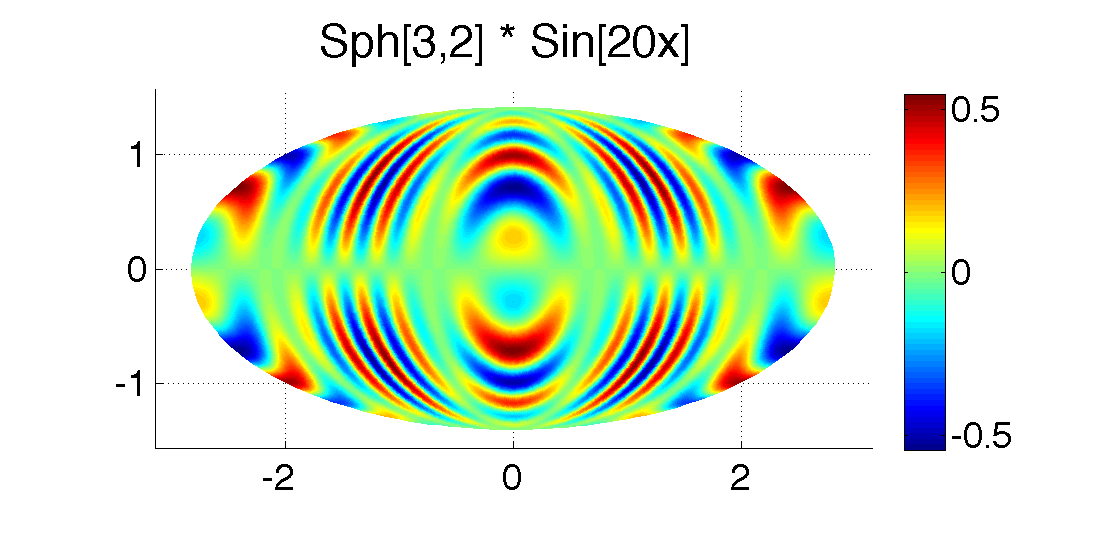
\includegraphics[width=1.0\textwidth]{../figures/appendices/direct_vs_indirect_weights/compare_weight_generation/xsfc_vs_xsfc_alt_on_sph32_times_sine_20x/sph32_times_sin20x.eps}
	\caption{Test function:  \\ $Y_{3}^{2} \sin(20 x) $.  }
	\end{subfigure}
	
	\begin{subfigure}[t]{0.48\textwidth}
		\centering
	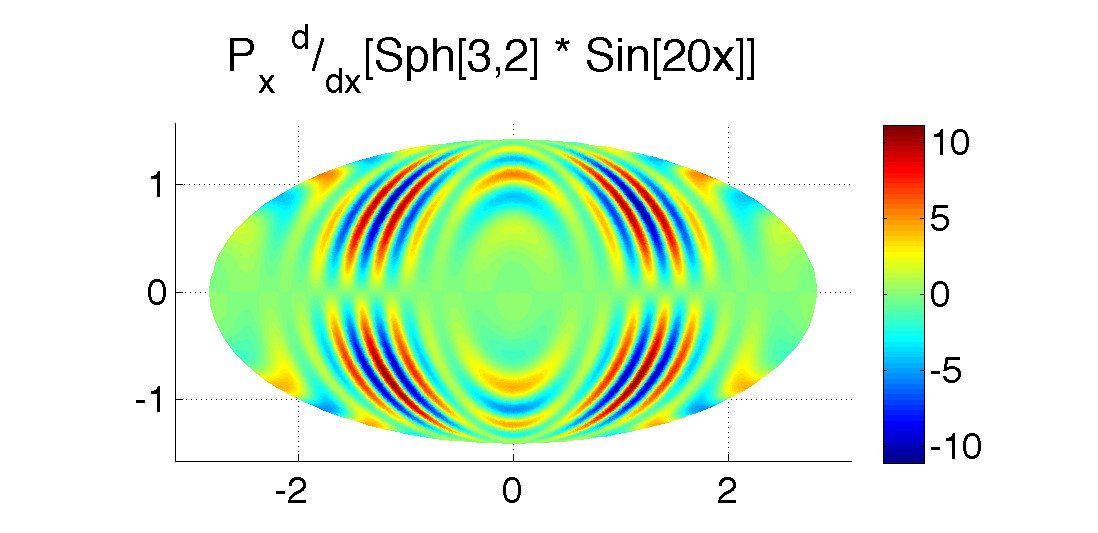
\includegraphics[width=1.0\textwidth]{../figures/appendices/direct_vs_indirect_weights/compare_weight_generation/xsfc_vs_xsfc_alt_on_sph32_times_sine_20x/pdx_sph32_times_sin20x.eps}
	\caption{$\mathbf{p}_{x} \cdot \nabla ( Y_{3}^{2} \sin(20 x))$ }
	\end{subfigure}
	\begin{subfigure}[t]{0.48\textwidth}
		\centering
	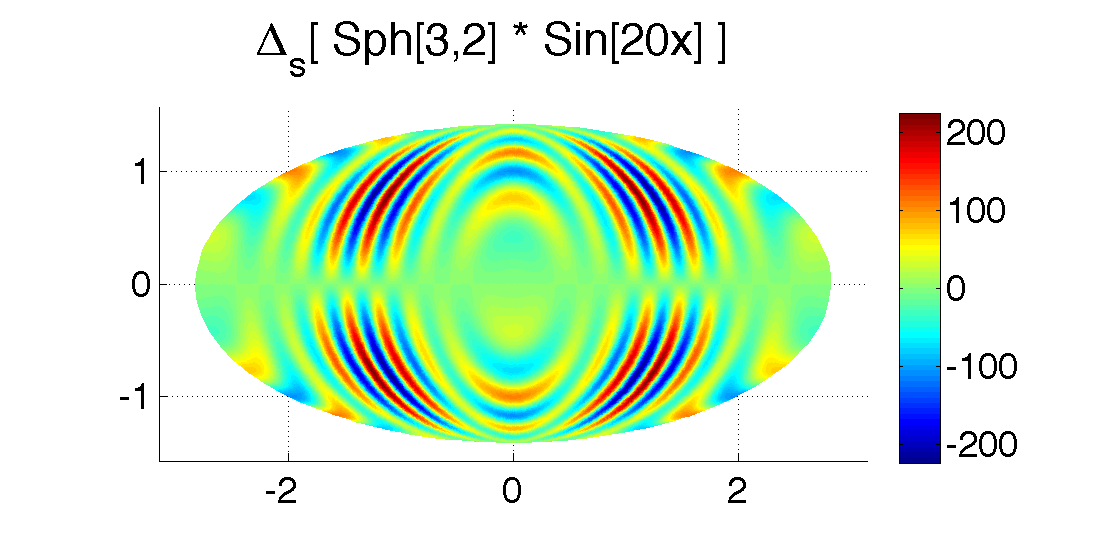
\includegraphics[width=1.0\textwidth]{../figures/appendices/direct_vs_indirect_weights/compare_weight_generation/lsfc_vs_px_grad_dot_px_grad/lsfc_sph32_times_sin20x.eps}
	\caption{Surface Laplacian: \\ $\LaplaceBeltrami ( Y_{3}^{2} \sin(20 x) )$  }
	\end{subfigure}
	\caption{Test function and its projected derivatives on the surface of the unit sphere. }
	\end{center}
\end{figure}

\begin{figure}
	\centering
	\begin{subfigure}[t]{0.48\textwidth}
	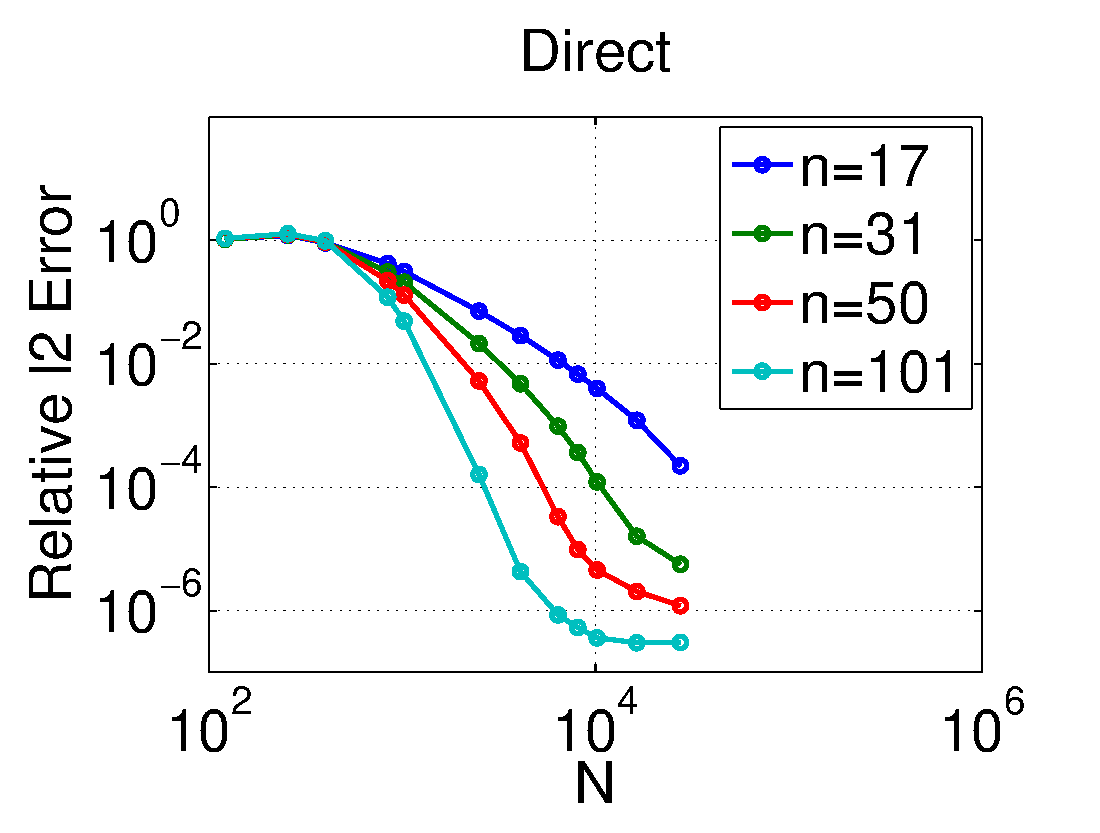
\includegraphics[width=1.0\textwidth]{../figures/appendices/direct_vs_indirect_weights/compare_weight_generation/xsfc_vs_xsfc_alt_on_sph32_times_sine_20x/direct_rel_l2_error.eps}
	\caption{$\mathbf{p}_{x} \cdot \nabla ( Y_{3}^{2} \sin(20 x))$ }
	\end{subfigure}
	\begin{subfigure}[t]{0.48\textwidth}
	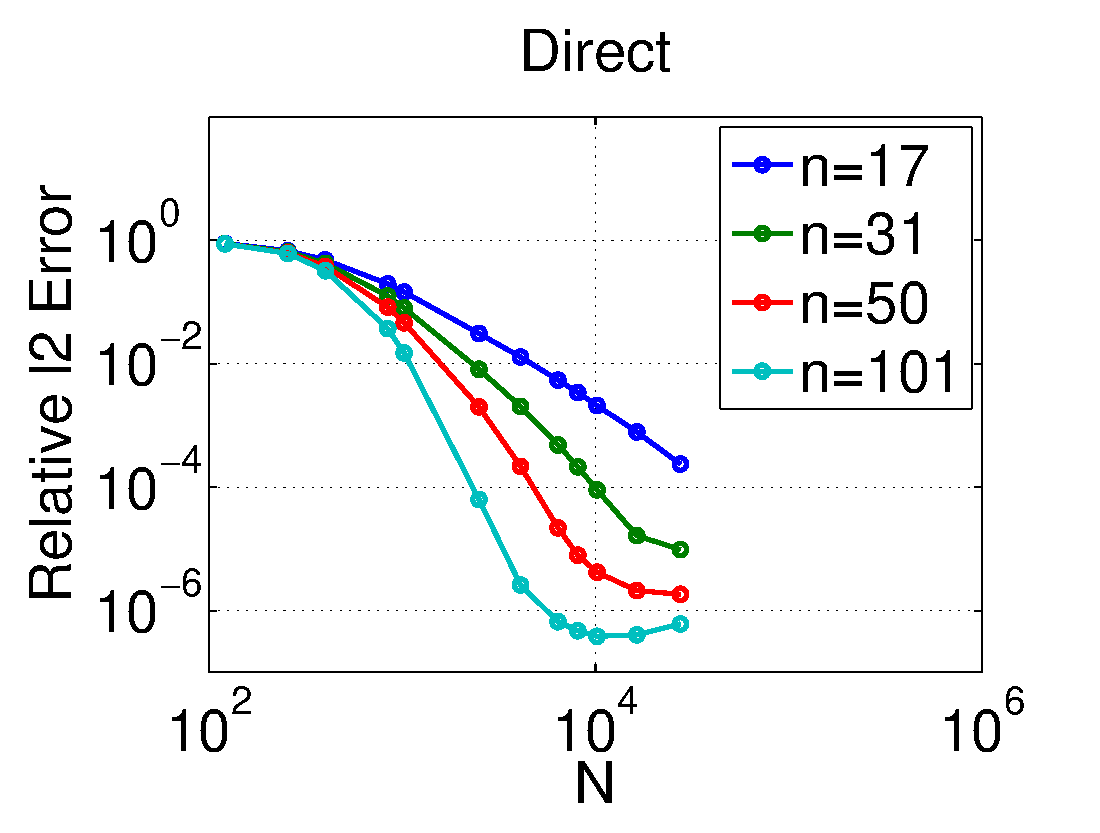
\includegraphics[width=1.0\textwidth]{../figures/appendices/direct_vs_indirect_weights/compare_weight_generation/lsfc_vs_px_grad_dot_px_grad/direct_rel_l2_error.eps}
	\caption{$\LaplaceBeltrami ( Y_{3}^{2} \sin(20 x) )$}
    \end{subfigure}
	\caption{Relative $\ell_{2}$ error in differentiation.}
\end{figure}


\begin{figure}
	\centering
	\begin{subfigure}[t]{0.48\textwidth}
	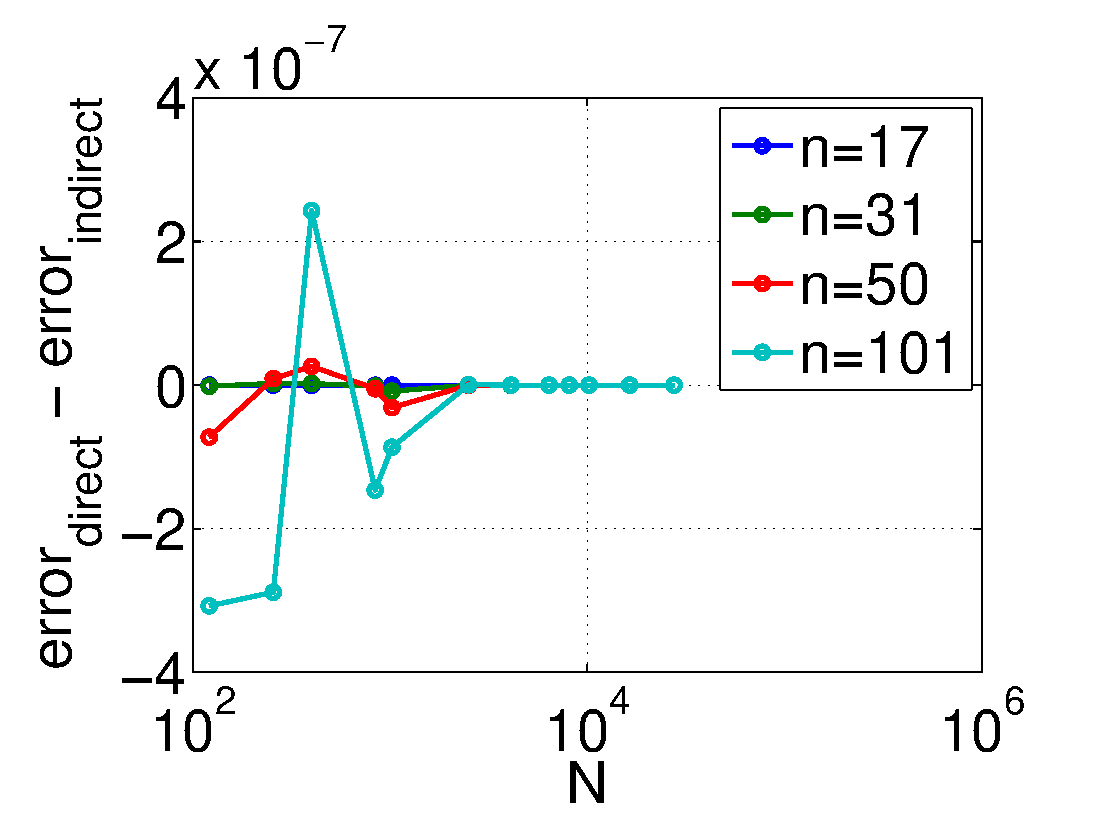
\includegraphics[width=1.0\textwidth]{../figures/appendices/direct_vs_indirect_weights/compare_weight_generation/xsfc_vs_xsfc_alt_on_sph32_times_sine_20x/diff_of_rel_l2_errors.eps}
	\caption{$\mathbf{p}_{x} \cdot \nabla ( Y_{3}^{2} \sin(20 x))$}
	\end{subfigure}
		\begin{subfigure}[t]{0.48\textwidth}
	\centering
	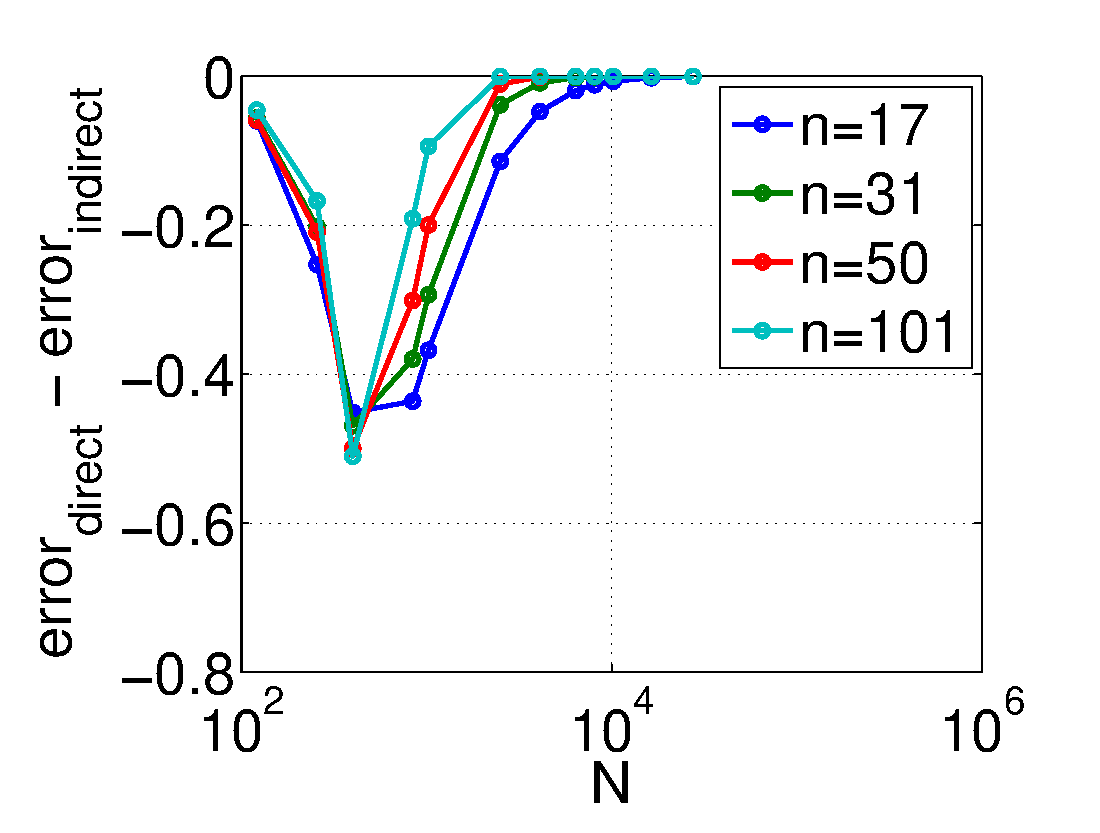
\includegraphics[width=1.0\textwidth]{../figures/appendices/direct_vs_indirect_weights/compare_weight_generation/lsfc_vs_px_grad_dot_px_grad/diff_of_rel_l2_errors.eps}
	\caption{$\LaplaceBeltrami ( Y_{3}^{2} \sin(20 x) )$ (Indirect error is significantly higher for small resolutions. This likely due to compounding errors from the operator $P_x (D_x D_x + D_y D_y + D_z D_z)$). Where negative this figure indicates that the error is higher for indirect weight calculation. }
	\end{subfigure}
	\caption{Signed differences of relative $\ell_{2}$ errors in differentiation between Direct and Indirect weights. The sign indicates on the error indicates the higher of the two weight approaches.}
\end{figure}


\begin{figure}
	\centering
		\begin{subfigure}[t]{0.48\textwidth}
		\centering
	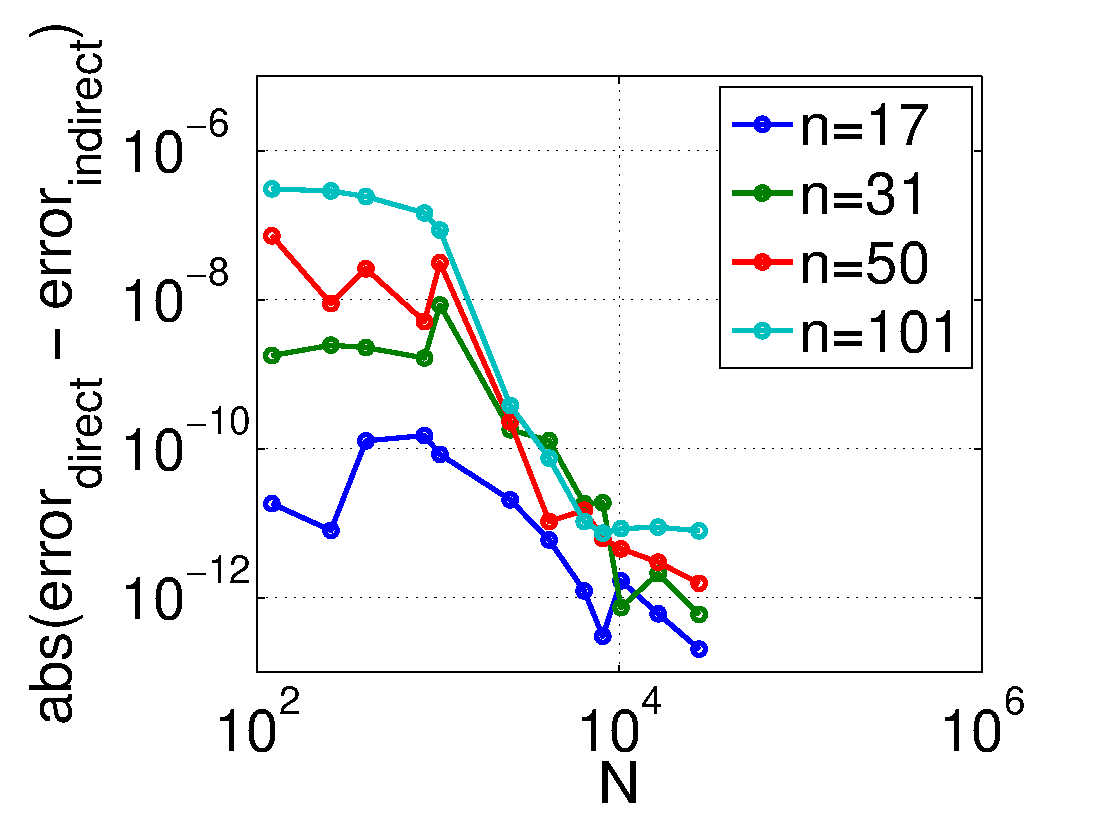
\includegraphics[width=1.0\textwidth]{../figures/appendices/direct_vs_indirect_weights/compare_weight_generation/xsfc_vs_xsfc_alt_on_sph32_times_sine_20x/abs_diff_of_rel_l2_errors.eps}
	\caption{$\mathbf{p}_{x} \cdot \nabla ( Y_{3}^{2} \sin(20 x))$}
	\end{subfigure}
	\begin{subfigure}[t]{0.48\textwidth}
	\centering
	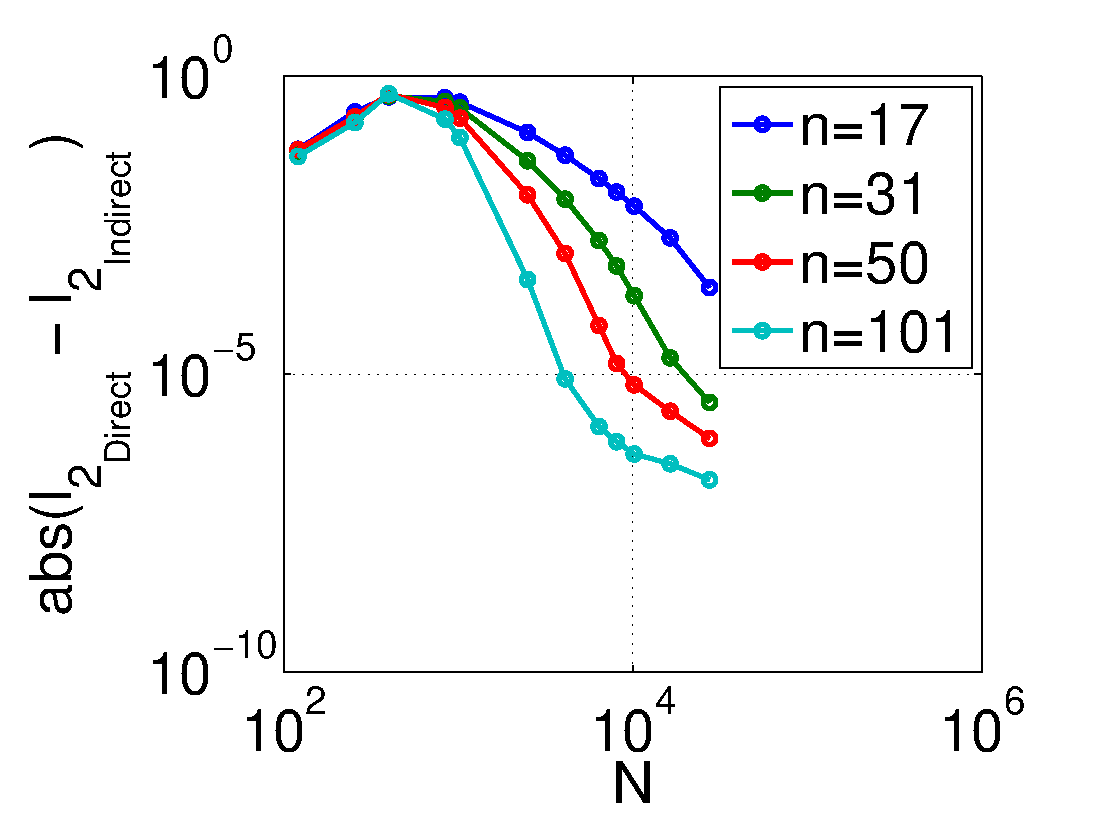
\includegraphics[width=1.0\textwidth]{../figures/appendices/direct_vs_indirect_weights/compare_weight_generation/lsfc_vs_px_grad_dot_px_grad/abs_diff_of_rel_l2_errors.eps}
	\caption{$\LaplaceBeltrami ( Y_{3}^{2} \sin(20 x) )$}
	\end{subfigure}
		\caption{Absolute differences of relative $\ell_{2}$ errors in differentiation between Direct and Indirect weights.}
\end{figure}

%% NOT USEFUL: %%
%\begin{figure}[htbp]
%\centering
%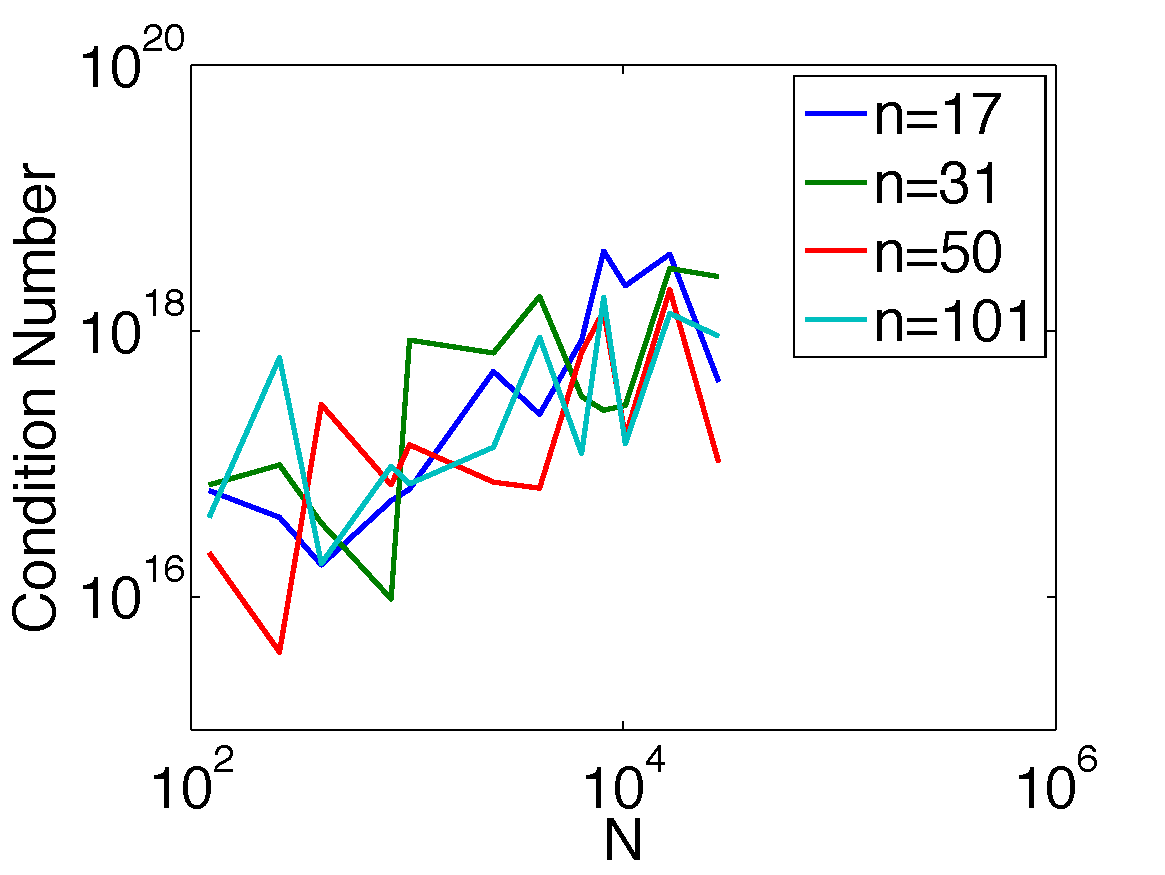
\includegraphics[width=0.425\textwidth]{../figures/chapter2/compare_weight_generation/xsfc_vs_xsfc_alt_on_sph32/condest_dm_xsfc.pdf}
%\caption{Condition number estimates (condest) of direct $\mathbf{p}_{x}\nabla$ differentiation matrix}
%\end{figure}


\section{Conclusions}

%TODO: It appears that indirect weight calculations function. 
%TODO: They do have potential for savings
%TODO: Low resolution amplifies the errors in indirect weights. 
%TODO: still need to compare with the RBF-GA stable weight methods. What if stable weights initially resolve the extra error we see for small resolutions?




%Although it is clear the indirect method functions well compared to the direct method, we must consider its usefulness. Typically, weights are computed only as necessary for a PDE. If the PDE is on the sphere, then directly computing the $\mathbf{P}\cdot \nabla$ operator would be most efficient for both memory and computation. However, one could imagine a scenario such as a 3-D spherical shell domain with physics on the boundaries that must be constrained to the surface, while the interior requires only an unprojected $\nabla$ operator. In such cases, by simply computing for the $\nabla$ operator, we assemble all necessary operators with minimal loss of accuracy and significant savings ($3Nn$ doubles) in storage. 


%\ifstandalone
%\bibliographystyle{plain}
%\bibliography{merged_references}
%\end{document}
%\else
%\expandafter\endinput
%\fi


\ifstandalone
\bibliographystyle{plain}
\bibliography{merged_references}
\end{document}
\else
\expandafter\endinput
\fi


\makeatletter
\@ifundefined{standalonetrue}{\newif\ifstandalone}{}
\@ifundefined{section}{\standalonetrue}{\standalonefalse}
\makeatother
\ifstandalone
\documentclass{report}

\usepackage{textcase}
%\usepackage{hyperref}
%\hypersetup{breaklinks=true}


% Added packages
\usepackage[usenames]{color}
\usepackage{amsfonts, amsmath, amssymb, graphics}

% NOTE: bibentry MUST appear before the hyperref or build will fail
\usepackage{bibentry}
\nobibliography*
\usepackage[square,sort,comma,numbers]{natbib}
  
\usepackage{float}
\usepackage[
	hidelinks,%
    %hyperindex=true,		% Make numbers of index links as well
   	backref=page, 		% Provide page listing where refs occur in the bibliography
	%breaklinks=true,
    %colorlinks,%
    %citecolor=green,%
    %filecolor=blue,%
    %linkcolor=red,%
    %urlcolor=red, 
]{hyperref}

\usepackage{dsfont}
%%%% USEPACKAGES for MACROS %%%%%
\usepackage{algpseudocode}
\usepackage[chapter]{algorithm}
%\usepackage{caption}
\usepackage{subcaption}
\usepackage{url}

\usepackage{array}
\usepackage{arydshln}
\usepackage{multirow}
\usepackage{multicol}
%\usepackage[section]{placeins}

\usepackage[usenames,dvipsnames]{color}
%\usepackage[english]{babel}
\usepackage{tabularx}
\usepackage{soul}
\usepackage{xparse}
\usepackage{listings}
%\usepackage[normalem]{ulem}



%%%%%%%%%%%%%%%
% Show a list of items "todo" or "done" 
% USAGE: 
% \begin{todolist} 
% 	\todo Something not finished
% 	\done Something finished
% \end{todolist} 
\newenvironment{todolist}{%
  \begin{list}{}{}% whatever you want the list to be
  \let\olditem\item
  \renewcommand\item{\olditem \textcolor{red}{(TODO)}: }
  \newcommand\todo{\olditem \textcolor{red}{(TODO)}: }
   \newcommand\done{\olditem \textcolor{ForestGreen}{(DONE)}: }
}{%
  \end{list}
} 
%%%%%%%%%%%%%%%

%%%%%%%%%%%%%%%
% Show a Author's Note
% USAGE: 
% \incomplete[Optional footnote message to further clarify note]{The text which is currently not finished}
\DeclareDocumentCommand \incomplete{ o m }
{%
\IfNoValueTF {#1}
{\textcolor{red}{Incomplete: \ul{#2}}} 
{\textcolor{red}{Incomplete: \ul{#2}}\footnote{Comment: #1}}%
}
%%%%%%%%%%%%%%%



%%%%%%%%%%%%%%%
% Show a Author's Note
% USAGE: 
% \authnote[Optional footnote message to further clarify note]{The note to your readers}
\DeclareDocumentCommand \authnote { o m }
{%
\IfNoValueTF {#1}
{\textcolor{blue}{Author's Note: \ul{#2}}} 
{\textcolor{blue}{Author's Note: \ul{#2}}\footnote{Comment: #1}}%
}
%%%%%%%%%%%%%%%



%%%%%%%%%%%%%%%
% Strike out text that doesn't belong in the paper
% USAGE: 
% \strike[Optional footnote to state why it doesn't belong]{Text to strike out}
\DeclareDocumentCommand \strike { o m }
{%
\setstcolor{Red}
\IfNoValueTF {#1}
{\textcolor{Gray}{\st{#2}}} 
{\textcolor{Gray}{\st{#2}}\footnote{Comment: #1}}%
}
%%%%%%%%%%%%%%%

\definecolor{light-gray}{gray}{0.95}

\newcommand{\cbox}[3]{
\ \\
\fcolorbox{#1}{#2}{
\parbox{\textwidth}{
#3
}
}
}

% Setup an environment similar to verbatim but which will highlight any bash commands we have
\lstnewenvironment{unixcmds}[0]
{
%\lstset{language=bash,frame=shadowbox,rulesepcolor=\color{blue}}
\lstset{ %
language=sh,		% Language
basicstyle=\ttfamily,
backgroundcolor=\color{light-gray}, 
rulecolor=\color{blue},
%frame=tb, 
columns=fullflexible,
%framexrightmargin=-.2\textwidth,
linewidth=0.8\textwidth,
breaklines=true,
%prebreak=/, 
  prebreak = \raisebox{0ex}[0ex][0ex]{\ensuremath{\hookleftarrow}},
%basicstyle=\footnotesize,       % the size of the fonts that are used for the code
%numbers=left,                   % where to put the line-numbers
%numberstyle=\footnotesize,      % the size of the fonts that are used for the line-numbers
%stepnumber=2,                   % the step between two line-numbers. If it's 1 each line 
                                % will be numbered
%numbersep=5pt,                  % how far the line-numbers are from the code
showspaces=false,               % show spaces adding particular underscores
showstringspaces=false,         % underline spaces within strings
showtabs=false,                 % show tabs within strings adding particular underscores
frame=single,	                % adds a frame around the code
tabsize=2,	                % sets default tabsize to 2 spaces
captionpos=b,                   % sets the caption-position to bottom
breakatwhitespace=false,        % sets if automatic breaks should only happen at whitespace
}
} { }

% Setup an environment similar to verbatim but which will highlight any bash commands we have
\lstnewenvironment{cppcode}[1]
{
%\lstset{language=bash,frame=shadowbox,rulesepcolor=\color{blue}}
\lstset{ %
	backgroundcolor=\color{light-gray}, 
	rulecolor=\color[rgb]{0.133,0.545,0.133},
	tabsize=4,
	language=[GNU]C++,
%	basicstyle=\ttfamily,
        basicstyle=\scriptsize,
        upquote=true,
        aboveskip={1.5\baselineskip},
        columns=fullflexible,
        %framexrightmargin=-.1\textwidth,
       %framexleftmargin=6mm,
        showstringspaces=false,
        extendedchars=true,
        breaklines=true,
        prebreak = \raisebox{0ex}[0ex][0ex]{\ensuremath{\hookleftarrow}},
        frame=single,
        showtabs=false,
        showspaces=false,
        showstringspaces=false,
        numbers=left,                   % where to put the line-numbers
	numberstyle=\footnotesize,      % the size of the fonts that are used for the line-numbers
	stepnumber=4,                   % the step between two line-numbers. If it's 1 each line 
                                % will be numbered
	firstnumber=#1,
         numbersep=5pt,                  % how far the line-numbers are from the code
        identifierstyle=\ttfamily,
        keywordstyle=\color[rgb]{0,0,1},
        commentstyle=\color[rgb]{0.133,0.545,0.133},
        stringstyle=\color[rgb]{0.627,0.126,0.941},
}
} { }

% Setup an environment similar to verbatim but which will highlight any bash commands we have
\lstnewenvironment{mcode}[1]
{
\lstset{ %
	backgroundcolor=\color{light-gray}, 
	rulecolor=\color[rgb]{0.133,0.545,0.133},
	tabsize=4,
	language=Matlab,
%	basicstyle=\ttfamily,
        basicstyle=\scriptsize,
        upquote=true,
        aboveskip={1.5\baselineskip},
        columns=fullflexible,
        %framexrightmargin=-.1\textwidth,
       %framexleftmargin=6mm,
        showstringspaces=false,
        extendedchars=true,
        breaklines=true,
        prebreak = \raisebox{0ex}[0ex][0ex]{\ensuremath{\hookleftarrow}},
        frame=single,
        showtabs=false,
        showspaces=false,
        showstringspaces=false,
        numbers=left,                   % where to put the line-numbers
	numberstyle=\footnotesize,      % the size of the fonts that are used for the line-numbers
	stepnumber=4,                   % the step between two line-numbers. If it's 1 each line 
                                % will be numbered
	firstnumber=#1,
         numbersep=5pt,                  % how far the line-numbers are from the code
        identifierstyle=\ttfamily,
        keywordstyle=\color[rgb]{0,0,1},
        commentstyle=\color[rgb]{0.133,0.545,0.133},
        stringstyle=\color[rgb]{0.627,0.126,0.941},
}
} { }

\newcommand{\inputmcode}[1]{%
\lstset{ %
	backgroundcolor=\color{light-gray},  %
	rulecolor=\color[rgb]{0.133,0.545,0.133}, %
	tabsize=4, %
	language=Matlab, %
%	basicstyle=\ttfamily,
        basicstyle=\scriptsize, %
        %        upquote=true,
        aboveskip={1.5\baselineskip}, %
        columns=fullflexible, %
        %framexrightmargin=-.1\textwidth,
       %framexleftmargin=6mm,
        showstringspaces=false, %
        extendedchars=true, %
        breaklines=true, %
        prebreak = \raisebox{0ex}[0ex][0ex]{\ensuremath{\hookleftarrow}}, %
        frame=single, %
        showtabs=false, %
        showspaces=false, %
        showstringspaces=false,%
        numbers=left,                   % where to put the line-numbers
	numberstyle=\footnotesize,      % the size of the fonts that are used for the line-numbers
	stepnumber=4,                   % the step between two line-numbers. If it's 1 each line 
                                % will be numbered
         numbersep=5pt,                  % how far the line-numbers are from the code
        identifierstyle=\ttfamily, %
        keywordstyle=\color[rgb]{0,0,1}, %
        commentstyle=\color[rgb]{0.133,0.545,0.133}, %
        stringstyle=\color[rgb]{0.627,0.126,0.941} %
}
\lstinputlisting{#1}%
}

%\lstset{ %
%	backgroundcolor=\color{light-gray}, 
%	rulecolor=\color[rgb]{0.133,0.545,0.133},
%	tabsize=4,
%	language=Matlab,
%%	basicstyle=\ttfamily,
%        basicstyle=\scriptsize,
%        upquote=true,
%        aboveskip={1.5\baselineskip},
%        columns=fullflexible,
%        %framexrightmargin=-.1\textwidth,
%       %framexleftmargin=6mm,
%        showstringspaces=false,
%        extendedchars=true,
%        breaklines=true,
%        prebreak = \raisebox{0ex}[0ex][0ex]{\ensuremath{\hookleftarrow}},
%        frame=single,
%        showtabs=false,
%        showspaces=false,
%        showstringspaces=false,
%        numbers=left,                   % where to put the line-numbers
%	numberstyle=\footnotesize,      % the size of the fonts that are used for the line-numbers
%	stepnumber=4,                   % the step between two line-numbers. If it's 1 each line 
%                                % will be numbered
%	firstnumber=#1,
%         numbersep=5pt,                  % how far the line-numbers are from the code
%        identifierstyle=\ttfamily,
%        keywordstyle=\color[rgb]{0,0,1},
%        commentstyle=\color[rgb]{0.133,0.545,0.133},
%        stringstyle=\color[rgb]{0.627,0.126,0.941},
%}


\newcommand{\Laplacian}[1]{\nabla^2 #1}

% set of all nodes received and contained on GPU
\newcommand{\setAllNodes}[0]{\mathcal{G}}
% set of stencil centers on GPU
\newcommand{\setCenters}[0]{\mathcal{Q}}
% set of stencil centers with nodes in \setDepend
\newcommand{\setBoundary}[0]{\mathcal{B}}
% set of nodes received by other GPUs
\newcommand{\setDepend}[0]{\mathcal{R}}
% set of nodes sent to other GPUs
\newcommand{\setProvide}[0]{\mathcal{O}}


\newcommand{\toprule}[0]{\hline}
\newcommand{\midrule}[0]{\hline\hline}
\newcommand{\bottomrule}[0]{\hline}

\newcolumntype{C}{>{\centering\arraybackslash}b{1in}}
\newcolumntype{L}{>{\flushleft\arraybackslash}b{1.5in}}
\newcolumntype{R}{>{\flushright\arraybackslash}b{1.5in}}
\newcolumntype{D}{>{\flushright\arraybackslash}b{2.0in}}
\newcolumntype{E}{>{\flushright\arraybackslash}b{1.0in}}

\DeclareSymbolFont{AMSb}{U}{msb}{m}{n}
\DeclareMathSymbol{\N}{\mathbin}{AMSb}{"4E}
\DeclareMathSymbol{\Z}{\mathbin}{AMSb}{"5A}
\DeclareMathSymbol{\R}{\mathbin}{AMSb}{"52}
\DeclareMathSymbol{\Q}{\mathbin}{AMSb}{"51}
\DeclareMathSymbol{\PP}{\mathbin}{AMSb}{"50}
\DeclareMathSymbol{\I}{\mathbin}{AMSb}{"49}
%\DeclareMathSymbol{\C}{\mathbin}{AMSb}{"43}

%%%%%% VECTOR NORM: %%%%%%%
\newcommand{\vectornorm}[1]{\left|\left|#1\right|\right|}
\newcommand{\vnorm}[1]{\left|\left|#1\right|\right|}
\newcommand{\by}[0]{\times}
\newcommand{\vect}[1]{\mathbf{#1}}
%\newcommand{\mat}[1]{\mathbf{#1}} 

%\renewcommand{\vec}[1]{ \textbf{#1} }
%%%%%%%%%%%%%%%%%%%%%%

%%%%%%% THM, COR, DEF %%%%%%%
%\newtheorem{theorem}{Theorem}[section]
%\newtheorem{lemma}[theorem]{Lemma}
%\newtheorem{proposition}[theorem]{Proposition}
%\newtheorem{corollary}[theorem]{Corollary}
%\newenvironment{proof}[1][Proof]{\begin{trivlist}
%\item[\hskip \labelsep {\bfseries #1}]}{\end{trivlist}}
%\newenvironment{definition}[1][Definition]{\begin{trivlist}
%\item[\hskip \labelsep {\bfseries #1}]}{\end{trivlist}}
%\newenvironment{example}[1][Example]{\begin{trivlist}
%\item[\hskip \labelsep {\bfseries #1}]}{\end{trivlist}}
%\newenvironment{remark}[1][Remark]{\begin{trivlist}
%\item[\hskip \labelsep {\bfseries #1}]}{\end{trivlist}}
%\newcommand{\qed}{\nobreak \ifvmode \relax \else
%      \ifdim\lastskip<1.5em \hskip-\lastskip
%      \hskip1.5em plus0em minus0.5em \fi \nobreak
%      \vrule height0.75em width0.5em depth0.25em\fi}
%%%%%%%%%%%%%%%%%%%%%%

%
%\usepackage[algochapter]{algorithm2e}
%\usepackage[usenames]{color}
% colors to show the corrections
\newcommand{\red}[1]{\textbf{\textcolor{red}{#1}}}
\newcommand{\blue}[1]{\textbf{\textcolor{blue}{#1}}}
\newcommand{\cyan}[1]{\textbf{\textcolor{cyan}{#1}}}
\newcommand{\green}[1]{\textbf{\textcolor{green}{#1}}}
\newcommand{\magenta}[1]{\textbf{\textcolor{magenta}{#1}}}
\newcommand{\orange}[1]{\textbf{\textcolor{orange}{#1}}}
%%%%%%%%%% DK DK
% comments between authors
\newcommand{\toall}[1]{\textbf{\green{@@@ All: #1 @@@}}}
\newcommand{\toevan}[1]{\textbf{\red{*** Evan: #1 ***}}}
%\newcommand{\toevan}[1]{}  % USE FOR FINAL VERSION
\newcommand{\toe}[1]{\textbf{\red{*** Evan: #1 ***}}}
\newcommand{\tog}[1]{\textbf{\blue{*** Gordon: #1 ***}}}
%\newcommand{\togordon}[1]{\textbf{\blue{*** Gordon: #1 ***}}}
\renewcommand{\ge}[3]{{\textcolor{blue}{*** \textbf{Gordon:}\strike{#1} #2 ***}}\red{(#3)}}
\renewcommand{\ge}[3]{{\textcolor{blue}{#2}}}
\renewcommand{\ge}[3]{{\textcolor{Red}{#2}}}
\newcommand{\eb}[3]{{\textcolor{Red}{*** \textbf{Evan:}\strike{#1} #2 ***}}\red{(#3)}}
\renewcommand{\eb}[3]{{{\textcolor{Red}{#2}}}}
%\def\ge#1#2#3{}{\textbf{\blue{*** Gordon: #2 ***}}}{(#3)}
\newcommand{\gee}[1]{{\bf{\blue{{\em #1}}}}}
\newcommand{\old}[1]{}
\newcommand{\del}[1]{***#1*** }



% \DeclareMathOperator{\Sample}{Sample}
%\let\vaccent=\v % rename builtin command \v{} to \vaccent{}
%\renewcommand{\vec}[1]{\ensuremath{\mathbf{#1}}} % for vectors
\newcommand{\gv}[1]{\ensuremath{\mbox{\boldmath$ #1 $}}} 
% for vectors of Greek letters
\newcommand{\uv}[1]{\ensuremath{\mathbf{\hat{#1}}}} % for unit vector
\newcommand{\abs}[1]{\left| #1 \right|} % for absolute value
\newcommand{\avg}[1]{\left< #1 \right>} % for average
\let\underdot=\d % rename builtin command \d{} to \underdot{}
\renewcommand{\d}[2]{\frac{d #1}{d #2}} % for derivatives
\newcommand{\dd}[2]{\frac{d^2 #1}{d #2^2}} % for double derivatives
\newcommand{\pd}[2]{\frac{\partial #1}{\partial #2}} 
% for partial derivatives
\newcommand{\pdd}[2]{\frac{\partial^2 #1}{\partial #2^2}} 
\newcommand{\pdda}[3]{\frac{\partial^2 #1}{\partial #2 \partial #3}} 
% for double partial derivatives
\newcommand{\pdc}[3]{\left( \frac{\partial #1}{\partial #2}
 \right)_{#3}} % for thermodynamic partial derivatives
\newcommand{\ket}[1]{\left| #1 \right>} % for Dirac bras
\newcommand{\bra}[1]{\left< #1 \right|} % for Dirac kets
\newcommand{\braket}[2]{\left< #1 \vphantom{#2} \right|
 \left. #2 \vphantom{#1} \right>} % for Dirac brackets
\newcommand{\matrixel}[3]{\left< #1 \vphantom{#2#3} \right|
 #2 \left| #3 \vphantom{#1#2} \right>} % for Dirac matrix elements
\newcommand{\grad}[1]{\gv{\nabla} #1} % for gradient
\let\divsymb=\div % rename builtin command \div to \divsymb
\renewcommand{\div}[1]{\gv{\nabla} \cdot #1} % for divergence
\newcommand{\curl}[1]{\gv{\nabla} \times #1} % for curl
\let\baraccent=\= % rename builtin command \= to \baraccent
\renewcommand{\=}[1]{\stackrel{#1}{=}} % for putting numbers above =
\newcommand{\diffop}[1]{\mathcal{L}#1}
\newcommand{\boundop}[1]{\mathcal{B}#1}
\newcommand{\rvec}[0]{{\bf r}}

\newcommand{\Interior}[0]{\Omega}
\newcommand{\domain}[0]{\Omega}
%\newcommand{\Boundary}[0]{\partial \Omega}
\newcommand{\Boundary}[0]{\Gamma}

\newcommand{\on}[1]{\hskip1.5em \textrm{ on } #1}

\newcommand{\gemm}{\texttt{GEMM}}
\newcommand{\trmm}{\texttt{TRMM}}
\newcommand{\gesvd}{\texttt{GESVD}}
\newcommand{\geqrf}{\texttt{GEQRF}}


\newcommand{\minitab}[2][l]{\begin{tabular}{#1}#2\end{tabular}}
\newcommand{\comm}[1]{\textcolor{red}{\textit{#1}}}

\newcommand{\nfrac}[2]{
\nicefrac{#1}{#2}
%\frac{#1}{#2}
}

\usepackage{xparse}
\usepackage{soul}


%%%%%%%%%%%%%%%
% Show a Author's Note
% USAGE: 
% \incomplete[Optional footnote message to further clarify note]{The text which is currently not finished}
\DeclareDocumentCommand \incomplete{ o m }
{%
\IfNoValueTF {#1}
{\textcolor{red}{Incomplete: \ul{#2}}} 
{\textcolor{red}{Incomplete: \ul{#2}}\footnote{Comment: #1}}%
}
%%%%%%%%%%%%%%%



%%%%%%%%%%%%%%%
% Show a Author's Note
% USAGE: 
% \authnote[Optional footnote message to further clarify note]{The note to your readers}
\DeclareDocumentCommand \authnote { o m }
{%
\IfNoValueTF {#1}
{\textcolor{blue}{Author's Note: \ul{#2}}} 
{\textcolor{blue}{Author's Note: \ul{#2}}\footnote{Comment: #1}}%
}
%%%%%%%%%%%%%%%



%%%%%%%%%%%%%%%
% Strike out text that doesn't belong in the paper
% USAGE: 
% \strike[Optional footnote to state why it doesn't belong]{Text to strike out}
\DeclareDocumentCommand \strike { o m }
{%
\setstcolor{red}
\IfNoValueTF {#1}
{\textcolor{Gray}{\st{#2}}} 
{\textcolor{Gray}{\st{#2}}\footnote{Comment: #1}}%
}
%%%%%%%%%%%%%%%



%
% colors to show the corrections
\newcommand{\red}[1]{\textbf{\textcolor{red}{#1}}}
\newcommand{\blue}[1]{\textbf{\textcolor{blue}{#1}}}
\newcommand{\cyan}[1]{\textbf{\textcolor{cyan}{#1}}}
\newcommand{\green}[1]{\textbf{\textcolor{green}{#1}}}
\newcommand{\magenta}[1]{\textbf{\textcolor{magenta}{#1}}}
\newcommand{\orange}[1]{\textbf{\textcolor{orange}{#1}}}
%%%%%%%%%% DK DK
% comments between authors
\newcommand{\toall}[1]{\textbf{\green{@@@ All: #1 @@@}}}
\newcommand{\toevan}[1]{\textbf{\red{*** Evan: #1 ***}}}
%\newcommand{\toevan}[1]{}  % USE FOR FINAL VERSION
\newcommand{\toe}[1]{\textbf{\red{*** Evan: #1 ***}}}
\newcommand{\tog}[1]{\textbf{\blue{*** Gordon: #1 ***}}}
%\newcommand{\togordon}[1]{\textbf{\blue{*** Gordon: #1 ***}}}
\renewcommand{\ge}[3]{{\textcolor{blue}{*** \textbf{Gordon:}\strike{#1} #2 ***}}\red{(#3)}}
\renewcommand{\ge}[3]{{\textcolor{blue}{#2}}}
\renewcommand{\ge}[3]{{\textcolor{red}{#2}}}
\newcommand{\eb}[3]{{\textcolor{red}{*** \textbf{Evan:}\strike{#1} #2 ***}}\red{(#3)}}
\renewcommand{\eb}[3]{{{\textcolor{red}{#2}}}}
%\def\ge#1#2#3{}{\textbf{\blue{*** Gordon: #2 ***}}}{(#3)}
\newcommand{\gee}[1]{{\bf{\blue{{\em #1}}}}}
\newcommand{\old}[1]{}
\newcommand{\del}[1]{***#1*** }



% Rename  this file          misc_mac.tex
%----------------------------------------------------------------------
%%%%%%%%%%%%%%%%%%%%%%%%%%%%%%%%%%%%%%%%%%%%%%%%%%%%%%%%%%%%%%%%%%%%%%%%%%%%%%%
%
%	Math Symbols   Math Symbols   Math Symbols   Math Symbols   
%
%%%%%%%%%%%%%%%%%%%%%%%%%%%%%%%%%%%%%%%%%%%%%%%%%%%%%%%%%%%%%%%%%%%%%%%%%%%%%%%
\def\pmb#1{\setbox0=\hbox{$#1$}%
	\kern-.025em\copy0\kern-\wd0
	\kern.05em\copy0\kern-\wd0
	\kern-.025em\raise.0433em\box0}
\def\pmbf#1{\pmb#1}
\def\bfg#1{\pmb#1}

% BETTER VALUES FOR AUTOMATIC FIGURE PLACEMENT THAN THOSE PROVIDED BY 
% LATEX DEFAULTS.

\renewcommand{\textfloatsep}{1ex}
\renewcommand{\floatpagefraction}{0.9}
\renewcommand{\intextsep}{1ex}
\renewcommand{\topfraction}{.9}
\renewcommand{\bottomfraction}{.9}
\renewcommand{\textfraction}{.1}

% #1  position of floating figure (h|t|b|p)
% #1  EPS postscript file
% #2  size
% #3  caption

%usage of newfig:
%  \newfig{file.ps}{3in}{Fig1: this is a figure}

\input{epsf}
\def\newfig#1#2#3{
  \begin{figure}[htbp]
  \vspace{1ex}
  \setlength{\epsfxsize}{#2}
  \centerline{\epsfbox{#1}}
  \vspace{-.1in}\caption{\small #3}\break\vspace{.2in}
  \label{#1}
  \end{figure}
}

%usage of newfigtwo: 2 figures, vertically stacked
% \newfig
%	{file1.ps}
%	{file2.ps}
%	{width}
%	{vertical space}
%	{Caption}

\def\newfigtwo#1#2#3#4#5{
  \begin{figure}[htbp]
  \vspace{1ex}
  \setlength{\epsfxsize}{#3}
  \centerline{\epsfbox{#1}}
  \vspace{#4}
  \setlength{\epsfxsize}{#3}
  \centerline{\epsfbox{#2}}
  \vspace{-.1in}\caption{\small #5}\break\vspace{.2in}
  \label{#1}
  \end{figure}
}

\def\newfigh#1#2#3#4{  % add height specification
  \begin{figure}[htbp]
  \vspace{1ex}
  \setlength{\epsfxsize}{#2}
  \setlength{\epsfysize}{#4}
  \centerline{\epsfbox{#1}}
  \vspace{-.1in}\caption{\small #3}\break\vspace{.2in}
  \label{#1}
  \end{figure}
}

\def\herefig#1#2#3{
  \begin{figure}[h]
  \setlength{\epsfxsize}{#2}
  \centerline{\epsfbox{#1}}
  \caption{\small #3}
  \label{#1}
  \end{figure}
}

\def\etal{{{\em et~al.\,\,}}}
\def\note#1{\\ =====#1===== \\}
\def\FBOX#1{\ \\ \fbox{\begin{minipage}{5in}#1\end{minipage}}\\ }
\newcount\sectionno     \sectionno=0
\newcount\eqnum         \eqnum=0
\def\addeqno{\global\advance \eqnum by  1 }
\def\subeqno{\global\advance \eqnum by -1 }
%\def\eqn{\addeqno \eqno \hbox{(\number\sectionno.\number\eqnum)} }

\def\tildetilde#1{\tilde{\tilde{#1}}}
\def\barbar#1{\overbar{\overbar{#1}}}

\def\vsp#1{\vspace{#1 ex}}
\def\fpar{\hspace{\parindent}}
%
%  \pf : 2 arguments: numerator and denominator of partial derivative
%
\def\pf#1#2{{\frac{\partial{#1}}{\partial{#2}}}}
\def\pfs#1#2{{\partial_{#2}{#1}}}
\def\pftwo#1#2{{\frac{\partial^2{#1}}{\partial{#2}^2}}}
\def\pfxx#1#2{{\frac{\partial^2{#1}}{\partial{#2}^2}}}
%\def\pfxy#1#2{{\frac{\partial^2{#1}}{\partial{#2}\partial{#3}}}}
\def\pfn#1#2#3{{\frac{\partial^{#1}{#2}}{\partial{#3}^{#1}}}}
\def\df#1#2{{\frac{d{#1}}{d{#2}}}}
\def\dfn#1#2#3{{\frac{d^{#1}{#2}}{d{#3}^{#1}}}}
\def\Dt#1#2{\frac{D#1}{D#2}}
\def\dt#1#2{\frac{d#1}{d#2}}
\def\bld#1{{\bf #1}}
\def\pfp#1#2#3{\pf{}{#3}{\left(\frac{#1}{#2}\right)}}

\def\norm#1{\|#1\|}

%
% Graphic characters  (\dot already defined by TeX/LateX)
%
\def\dash{\rule[1.5pt]{2mm}{.3mm}\HS{.9mm}}
\def\dott{\rule[1.5pt]{.7mm}{.3mm}\HS{.7mm}}
\def\dashline{\dash\dash\dash}
\def\dotline{\dott\dott\dott\dott\dott\dott}
\def\dashdotline{\dash$\cdot$\HS{.9mm}\dash}
\def\solidline{\rule[2pt]{7mm}{.3mm}}
% 
% overcircle
%
\def\ovcircle#1{\buildrel{\circ}\over{#1}}
%\def\below#1#2{\buildrel{#2}\under{#1}}
%\def\above#1#2{\buildrel{#2}\over{#1}}
%
%  big parenthesis and brackets
%
\def\bigpar#1#2{{\left(\frac{#1}{#2}\right)}}
\def\bigbra#1#2{{\left\[\frac{#1}{#2}\right\]}}

\def\Lp{\left(}
\def\Rp{\right)}
\def\Lb{\left[}
\def\Rb{\right]}
\def\Ln{\left\langle}
\def\Rn{\right\rangle}
\def\Ld{\left.}
\def\Rd{\right.}
\def\Lv{\left|}
\def\Rv{\right|}
\def\Lbr{\left|}
\def\Rbr{\right|}
\def\lng{\langle}
\def\rng{\rangle}
\def\Lc{\left\{}
\def\Rc{\right\}}
%%% %

% Cannot be handled by Lyx
%\def\[{{[}}
%\def\]{{]}}

%
\def\eol{\nonumber \\}
\def\eolnonb{\nonumber\\}
\def\eolnb{\\}
\def\nonb{\nonumber}
\def\be{\begin{equation}}
\def\ee{\end{equation}}
\def\BEQNA{\begin{eqnarray}}
\def\EEQNA{\end{eqnarray}}
\def\eqa{&=&}
\def\beqna{\begin{eqnarray}}
\def\eeqna{\end{eqnarray}}
\def\bverb{\begin{verbatim}}
\def\everb{\end{verbatim}}
\def\VERB#1{\bverb #1 \everb}
\def\btbl{\begin{tabular}}
\def\etbl{\end{tabular}}
\def\bmini{\begin{minipage}[t]{5.5in}}
\def\emini{\end{minipage}}
\def\parray#1#2{\left(\begin{array}{#1}#2\end{array}\right)}
\def\barray#1#2{\left[\begin{array}{#1}#2\end{array}\right]}
\def\carray#1#2{\left\{\begin{array}{#1}#2\end{array}\right.}
\def\darray#1#2{\left|\begin{array}{#1}#2\end{array}\right|}

\def\BEGTABLE#1{\begin{table}[hbt]\vspace{2ex}\begin{center}\bmini\centering\btbl{#1}}
\def\ENDTABLE#1#2{\etbl\caption[#1]{#2}\EMINI\end{center}\vspace{2ex}\end{table}}

\def\bfltbl#1{\begin{table}[hbt]\vspace{2ex}\begin{center}\bmini\centering\btbl{#1}}
\def\efltbl#1#2{\etbl\caption[#1]{#2}\emini\end{center}\vspace{2ex}\end{table}}
\def\mcol{\multicolumn}
%
%  label equations with (#)
%
\def\reff#1{(\ref{#1})}
%
%  macros borrowed from viewgraph package
%

\newenvironment{LETTRS}[3]{\begin{letter}{#1}
\input{origin}\opening{Dear #2:}\input{#3}\closing{Sincerely yours,}\end{letter}}{\clearpage}

\newenvironment{VIEW}[1]{{\BC\Huge\bf #1 \EC}\LARGE\VS{.05in}}{\clearpage}

\def\RM#1{\rm{#1\ }}
\def\BV{\begin{VIEW}}
\def\EV{\end{VIEW}}

\def\NI{\noindent}

\def\VS{\vspace*}
\def\HS{\hspace*}
\def\IT{\item}

\def\BARR{\begin{array}}
\def\EARR{\end{array}}

\def\BPARR{\left(\begin{array}}
\def\EPARR{\end{array}\right)}

\def\BDET{\left|\begin{array}}
\def\EDET{\end{array}\right|}

\def\BDF{\begin{definition}}
\def\EDF{\end{definition}}

\def\BSU{\begin{block}{Summary}}
\def\ESU{\end{block}}

\def\BEX{\begin{example}}
\def\EEX{\end{example}}

\def\BTH{\begin{theorem}}
\def\ETH{\end{theorem}}

\def\BCO{\begin{corollary}}
\def\ECO{\end{corollary}}

\def\BPROOF{\begin{proof}}
\def\EPROOF{\end{proof}}

\def\BLM{\begin{lemma}}
\def\ELM{\end{lemma}}

\def\BEQ{\begin{equation}}
\def\EEQ{\end{equation}}

\def\BEQNNB{$$}
\def\EEQNNB{$$}

\def\BE{\begin{enumerate}}
\def\EE{\end{enumerate}}

\def\BD{\begin{description}}
\def\ED{\end{description}}

\def\BI{\begin{itemize}}
\def\EI{\end{itemize}}

\def\BC{\begin{center}}
\def\EC{\end{center}}

\def\BFIG{\begin{figure}}
\def\EFIG{\end{figure}}

\def\BTABB{\begin{tabbing}}
\def\ETABB{\end{tabbing}}

\def\BMINI{\begin{minipage}}
\def\EMINI{\end{minipage}}

\def\BTABLE{\begin{table}}
\def\ETABLE{\end{table}}

\def\BTABUL{\begin{tabular}}
\def\ETABUL{\end{tabular}}

\def\MCOL{\multicolumn}
\def\UL{\underline}
\def\ULL#1{\UL{\UL{#1}}}

\def\BDOC{\begin{document}}
\def\EDOC{\end{document}}

\def\EM#1{{\em #1\/}}
\def\FN{\footnote}

% Courtesy of Ugo Piomelli

\def\latexfig #1 #2 #3 #4 #5 {\ \vfill
\hfill\hbox to 0.05in{\vbox to #3truein{
         \special{psfile="#1" angle=270 hscale=100 
                  hoffset=#4 voffset=#5 vscale=100} }\hfill}
\hfill\vspace{-0.1in}        }

% #1 is the .ps filename
% #2 is not used in the present version
% #3 is the size of the white space left above the caption (in inches)
% #4 is the horizontal offset from some unknown reference point.
%    It is in 1/72 of an inch and is positive to the right.
% #5 is the vertical offset from some unknown reference point.
%    It is in 1/72 of an inch and is positive upwards.


\newcommand{\mathsym}[1]{{}}
\newcommand{\unicode}[1]{{}}
\newcommand{\ep}{\epsilon}
\newcommand{\vv}{\mathbf{v}}
\newcommand{\vu}{\mathbf{u}}
\newcommand{\vx}{\mathbf{x}}

\newcommand{\Laplacian}[1]{\nabla^2 #1}
\newcommand{\LaplaceBeltrami}[1]{\Delta_S #1}

% set of all nodes received and contained on GPU
\newcommand{\setAllNodes}[0]{\mathcal{G}}
% set of stencil centers on GPU
\newcommand{\setCenters}[0]{\mathcal{Q}}
% set of stencil centers with nodes in \setDepend
\newcommand{\setBoundary}[0]{\mathcal{B}}
% set of nodes received by other GPUs
\newcommand{\setDepend}[0]{\mathcal{R}}
% set of nodes sent to other GPUs
\newcommand{\setProvide}[0]{\mathcal{O}}





\usepackage{tabularx} 
\newcolumntype{C}{>{\centering\arraybackslash}b{1in}}
\newcolumntype{L}{>{\flushleft\arraybackslash}b{1.5in}}
\newcolumntype{R}{>{\flushright\arraybackslash}b{1.5in}}
\newcolumntype{D}{>{\flushright\arraybackslash}b{2.0in}}
\newcolumntype{E}{>{\flushright\arraybackslash}b{1.0in}}


 


%\usepackage{xcolor}

%\usepackage{refcheck}
% Sepia
%\definecolor{myBGcolor}{HTML}{F6F0D6}
%\definecolor{myTextcolor}{HTML}{4F452C}
% Dark
%\definecolor{myBGcolor}{HTML}{3E3535}
%\definecolor{myTextcolor}{HTML}{CFECEC}
%\color{myTextcolor}
%\pagecolor{myBGcolor}
 

\begin{document}
\fi




\chapter{An Alternative Stencil Generation Algorithm for RBF-FD}
\label{chap:stencils}

Like all RBF methods, RBF-FD is designed to handle irregular node distributions, so the emphasis in the literature focuses on how the method manages point clouds. While nothing prevents implementations of RBF-FD from utilizing existing meshes/lattices, most work in the field concentrates on simple geometries to better understand properties of the method and develop extensions. Without mesh/lattice connectivity available, stencils are generated by choosing the $n$-nearest neighbors to a center node, inclusive of the center. This is known more formally as a \emph{$k$-nearest neighbor (k-NN)} problem \cite{TagliasacchiMFE} (a.k.a. $\ell$-nearest neighbor search \cite{WendlandBook}). Here ``nearest" is defined with the Euclidean distance metric, although it is possible to generalize to other metrics (see e.g., \cite{MatlabKDTreeSearcher}). 

Compared to the RBF-FD method, global RBF methods with infinite support connect all nodes to all other nodes, so there is no need for neighbor queries. On the other hand, compact RBF methods require all nodes---with no limit on the count---that lie within the support/radius of the RBF centered at each node. This type of neighbor query is referred to as a \emph{ball query} (a.k.a. range query \cite{WendlandBook}) due to the closed ball created by the radius of support for a compact RBF (see Equation~\ref{eqn:csrbf}). 

The $k$-NN and ball query share many similarities, but the former is harder to solve. Consider, for example, the scenario in Figure~\ref{fig:nearest_neighbor_example}. Two ball queries around a blue stencil center are represented as dashed and dash-dot circles. The inner query returns four neighbors, and the outer returns six. If a stencil of size $n=6$ is desired, then the outer query can be truncated to give the five required neighbors shown in blue. In this example the red node and the farthest blue node are equidistant from the center, and ties are broken arbitrarily. Although $k$-NN is simply a truncated ball query, the real challenge lies in finding the proper search radius to enclose at least the $n$ desired neighbors. To find the radius in practice depends on the choice of data structure used to access node locations. 

\begin{figure}
\centering
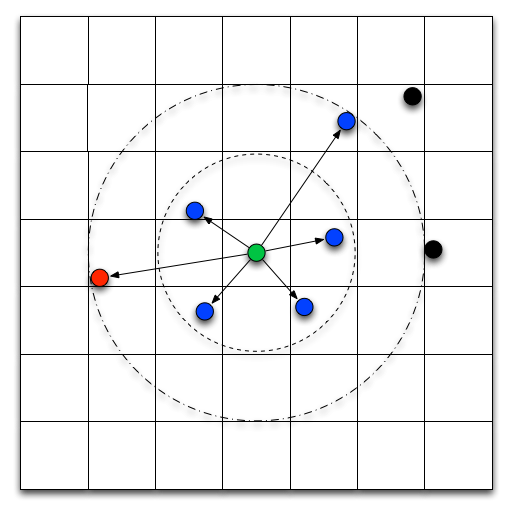
\includegraphics[width=5.5cm]{rbffd_methods_content/neighbors/ball_query_vs_kNN.png}
\caption{A stencil center in blue finds neighboring stencil nodes in blue. Two ball queries are shown as dashed and dash-dot circles to demonstrate the added difficulty of finding the right query radius to obtain the $k$-nearest neighbors.}
\label{fig:nearest_neighbor_example}
\end{figure}


A na\"{i}ve approach for neighbor queries would be a brute-force search that checks distances from all nodes to every other node. Obviously the cost of such a method is high: $O(N^2)$ for all stencils. Multi-dimensional data structures, such as those discussed here, can limit the scope of searching and reduce the cost of stencil generation to $O(N \log{N})$. 

For the most part, investigations in RBF communities that delve into efficient neighbor queries are limited to ball queries, for example, the Partition of Unity method for approximation (e.g., \cite{Wendland2002,WendlandBook}), and particle methods such as the Fast Multipole Method (e.g., \cite{Ying2006, Gumerov2003}) or Smoothed Particle Hydrodynamics (e.g., \cite{Krog2010}). Examples of fast algorithms employed in these fields include the fixed-grid method \cite{WendlandBook,Krog2010}, $k$-D Trees \cite{WendlandBook}, Range Trees \cite{Wendland2002,WendlandBook}, and $2^d$-Trees (i.e., Quad- and Octrees) \cite{Gumerov2003, Ying2006}. Surprisingly, while other communities continue the quest for fast neighbor queries, RBF collocation and RBF-FD communities have been slow on the uptake. For many years, the standard in the community has been to use $k$-D Trees (see e.g., \cite{Fasshauer2007, FlyerLehto11,FornbergLehto11}). 


This chapter considers the use of an alternative neighbor query algorithm to generate RBF-FD stencils. It is based loosely on the fixed-grid method from \cite{Krog2010,Green2010,Johnson2011}. Samet\cite{Samet2005} would classify the algorithm as a \emph{fixed grid ``bucket" method with one-dimensional spatial ordering}. The fixed-grid method loosens the requirements for finding the $k$-nearest neighbors ($k$-NN) stencils to accept $k$-``approximately nearest" neighbors ($k$-ANN). It also reorders nodes according to space-filling curves. In what follows, the fixed-grid method is compared to an efficient implementation of $k$-D Tree available for use in C++ and MATLAB (\cite{TagliasacchiMFE}). Benchmarks in \S~\ref{sec:fixed_grid_benchmarks} demonstrate that, with the proper choice of parameters for the fixed-grid, the method can be up to 2x faster than $k$-D Tree, and it comes with a free bonus: up to 5x faster SpMV performance due to the impact of spatial reordering that occurs during stencil generation. 


\section{$k$-D Tree}

A $k$-D Tree is a spatial data structure that generally decomposes a space/volume into a small number of cells. All $k$-D Trees are binary and iteratively partition volumes and sub-volumes at each level into two parts. The ``$k$" in $k$-D Tree refers to the dimensionality of the data/volume  partitioned---that is $k \equiv d$. 


Given a set of points bounded by a $d$-dimensional volume, a $k$-D Tree applies a hierarchy of $(d-1)$-dimensional axis aligned \emph{splitting planes} to cut the space. At each level of the hierarchy the splitting planes result in two new \emph{half-planes} \cite{Skiena2008}. Consecutive splits intercept one another at a \emph{splitting value}. $k$-D Trees do not require that half-planes equally subdivide a volume; more often it is the data contained within the volume that is equally partitioned. The choice of dimension for the splitting plane, in conjunction with a variety of methods for choosing the splitting values allows for many flavors of $k$-D Trees (see e.g., \cite{Samet2005, Skiena2008, Berg2008} for comprehensive lists). \emph{Point $k$-D Trees}, \emph{$2^d$ Trees} (i.e., quad-/octrees), \emph{BSP-Trees}, and \emph{R-trees} are all members of the general $k$-D Tree class \cite{Skiena2008,Ying2006}.

This work considers \emph{Point $k$-D Trees} \cite{Samet2005}, which partition a set of discrete points/nodes as outlined by the recursive procedure in Algorithm~\ref{alg:kdtree_build}. Point $k$-D Trees assume that splitting planes intercept at node coordinates rather than occur arbitrarily along the half-plane. The splitting value at each level of the tree is set to the \emph{median coordinate} of the points in the half-plane, which ensures that the tree is well balanced on construction. All nodes with coordinate (in the current dimension) less than or equal to the splitting value are contained by the left half-plane, and all nodes with coordinate greater than the splitting value are contained by the right. Half-planes containing only one element correspond to leaves of the tree. The median coordinate of a half-plane is found by sorting the $n$ node coordinates contained by the partition and selecting the $\left\lceil \frac{n}{2} \right\rceil$-th element \cite{Berg2008}. 
\begin{algorithm} 
\caption{BuildKDTree($P$, $depth$)}         \label{alg:kdtree_build}  
\begin{algorithmic}[1]    
    \State \textbf{Input:} A set of $d$-dimensional points $P$ and the current $depth$.
    \State \textbf{Output:} The root of the $k$-D Tree for $P$.
    \State
    \If{$size(P) = 1$}
    \State \Return a new leaf storing $P$
    \EndIf
    \State $L_i := median(coord(P, depth))$ 
    \State $v_{l} := $ BuildKDTree($coord(P, depth) \leq L_i$, $(depth+1)$ modulo $d$)
    \State $v_{r} := $ BuildKDTree($coord(P, depth) > L_i$, $(depth+1)$ modulo $d$) 
    \State \Return A new node $v := \begin{pmatrix} \text{value} := L_i \\ \text{left} := v_l \\ \text{right} := v_r \end{pmatrix}$ 
\end{algorithmic}
\end{algorithm}

The $k$-D Tree in Figure~\ref{fig:kdtree_example} is an example of a Point $k$-D Tree. Given a set of eight nodes in two dimensions, the tree is constructed by applying one-dimensional cuts along the $x$-dimension, then the $y$-dimension, then back to the $x$-dimension. This approach is referred to as \emph{cyclic splitting}, as consecutive cuts are applied by iterating dimensions in a round-robin fashion \cite{Samet2005}. The first cut, $L1$, shown in blue, splits the nodes into two sets on either side of $A$. The corresponding tree in the center of Figure~\ref{fig:kdtree_example} shows $L1$ as the tree root with all nodes having $x$-coordinates less than or equal to $A$ to the left, and all nodes having $x$-coordinates greater than $A$ to the right. The second level of the tree, $L2$ and $L3$ (in blue), splits the half-planes on either side of $A$ at nodes $B$ and $C$. The axis parallel splits for each half-plane intercept $L1$ independently to partition half-planes along the $y$-dimension; once again, nodes with coordinates less than or equal (i.e., below) to the splitting value branch left in the tree, and $y$-coordinates greater than  (i.e., above) the value branch right. The third level (red) returns to splitting half-planes in the $x$-dimension. Nodes $D$ and $H$ are not intersected by a splitting plane; their half-planes contain only one node so they immediately become leaves of the tree. This process to build a Point $k$-D Tree has a complexity of $O(N \log N)$ with $O(N)$ storage \cite{Berg2008,Samet2005}.

\begin{figure}
\centering
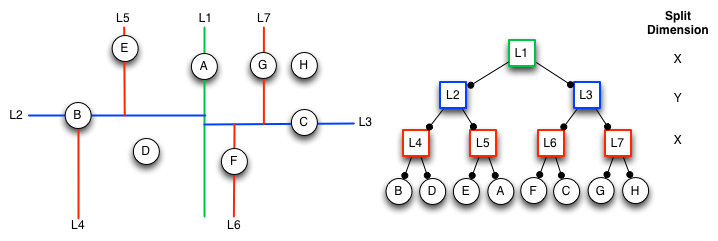
\includegraphics[width=0.9\textwidth]{rbffd_methods_content/neighbors/kdTree_example.png}
\caption{An example $k$-D Tree in 2-Dimensions. Nodes are partitioned with a cyclic dimension splitting rule (i.e., splits occur first in $X$, then $Y$, then $X$, etc.); all splits occur at the median node in each dimension. }
\label{fig:kdtree_example}
\end{figure}

Frequently, the terms \emph{$k$-D Tree} and \emph{Point $k$-D Tree} are used synonymously by the RBF community (see e.g., \cite{Fasshauer2007,FlyerLehto11,FornbergLehto11}); the same convention is adopted here. 

Generating an RBF-FD stencil with a $k$-D Tree can be efficiently accomplished in $O(n \log{N})$ time---where $n$ is the stencil size---following an approach introduced in \cite{Friedman1977}, and presented in Algorithm~\ref{alg:kdtree_knn}. The $k$-NN search starts a depth-first recursive search of the $k$-D Tree to find the nearest neighbor to a query point, $X_q$. Traversal of the the tree occurs by following branches left or right based on comparison of $X_q$ coordinates to the splitting value stored at each node of the tree, with the objective to find the smallest half-plane containing $X_q$. The search traverses the height of the tree in $O(\log N)$ steps to find the leaf that stores the nearest neighbor to $X_q$. The neighbor point and its distance from $X_q$ are inserted into a global priority queue, $pq$. Points in the priority queue are sorted in descending order according to distance. 


\begin{algorithm} 
\caption{KNNSearchKDTree($X_q$, $n$, $root$, $depth$)}         \label{alg:kdtree_knn}  
\begin{algorithmic}[1]    
    \State \textbf{Input:} A query node $X_q$, number of desired neighbors ($n$), the current \emph{root} of the $k$-D Tree, and the current $depth$ of traversal.
    \State \textbf{Output:} A global priority queue, $pq$, containing the $n$-nearest neighbors to $X_q$ sorted by distance from $X_q$ in descending order.
    \State \textbf{Assume:} A routine named ``BoundsOverlapBall" exists to determine if the boundaries of the current half-plane are intersected by the ball centered at $X_q$ with radius equal to the maximum distance in $pq$. As long as $pq.size < n$, ``BoundsOverlapBall" defaults to true. %$B_{+}$ and $B_{-}$ are $d$-dimensional arrays initialized to $\pm \infty$ on first call and used within BoundsOverlapBall.
    \State
    \If{$root$ is leaf}
        \State Insert $\{root,\text{dist}(X_q,root)\}$ into $pq$
        \If{$pq.\text{size} > n$} 
            \State $pq$.pop \Comment{Keep only $n$-nearest neighbors}
        \EndIf
        \State \Return
    \EndIf
    \State
    \If{$\text{coord}(X_q, depth) <= root.\text{value}$} 
       % \State $temp := B_{+}[depth]$, and $B_{+}[depth] := root.\text{value}$
        \State KNNSearchKDTree($X_q$, $n$, $root.\text{left}$, $(depth+1) \text{ \% } d$)
       % \State $B_{+}[depth] := temp$
    \Else
        %\State $temp := B_{-}[depth]$, and $B_{-}[depth] := root.\text{value}$
        \State KNNSearchKDTree($X_q$, $n$, $root.\text{right}$, $(depth+1) \text{ \% } d$)
       % \State $B_{-}[depth] := temp$
    \EndIf
    \State 
    \If{$\text{coord}(X_q, depth) <= root.\text{value}$} 
        %\State $temp := B_{-}[depth]$, and $B_{-}[depth] := root.\text{value}$
        \If{BoundsOverlapBall($X_q$)}
            \State KNNSearchKDTree($X_q$, $n$, $root.\text{right}$, $(depth+1) \text{ \% } d$)
        \EndIf
        %\State $B_{-}[depth] := temp$
    \Else
        %\State $temp := B_{-}[depth]$, and $B_{-}[depth] := root.\text{value}$
        \If{BoundsOverlapBall($X_q$)}
            \State KNNSearchKDTree($X_q$, $n$, $root.\text{left}$, $(depth+1) \text{ \% } d$)
        \EndIf
        %\State $B_{+}[depth] := temp$
    \EndIf
    \State \Return
    \end{algorithmic}
\end{algorithm}

After finding the nearest neighbor the algorithm returns to the previous split in the tree and traverses onto the opposing half-plane (i.e., down the far branch) to look for other leaves. So long as the size of $pq$ is at less than capacity ($n$) the search automatically adds points to the priority queue. If $pq$ reaches capacity the algorithm starts to pop off excess points with the understanding that the action removes those points farthest from $X_q$. 

In order to prune branches from the search and reduce complexity, Algorithm~\ref{alg:kdtree_knn} makes use of a routine called ``BoundsOverlapBall", which checks if any boundaries of the current level half-plane intersect/overlap with a closed ball centered at $X_q$. The ball is given a radius equal to the maximum distance in $pq$. Then, if the ball and a boundary intersect, the search will continue onto the half-plane on the opposite side of that boundary. This step handles the possibility that nearer nodes occur within the overlapped region in the other half-plane. If the ball and boundary do not intersect, the opposing half-plane and its related subtree are pruned from the search. Additional details on the implementation of ``BoundsOverlapBall" can be found in \cite{Friedman1977,TagliasacchiGC}. 

The authors of \cite{Friedman1977} find Algorithm~\ref{alg:kdtree_knn} capable of efficiently querying the $n$-nearest neighbors with a complexity proportional to $O(\log{N})$ (dominated by the cost of tree traversal). %The relationship between stencil size $n$, and grid size, $N$, is better expressed as $O(n \log{N})$ for one stencil. 

RBF-FD only needs to generate stencils once, so the overall time for stencil generation subsumes the cost of tree construction and $N$ queries. The resulting total complexity of stencil generation for all stencils is thus proportional to $O(N\log{N})$. %The implementation of $k$-D Tree tested in Section~\ref{sec:stencils_benchmarks} reflects this complexity. 


% TODO: other related work. What implementations are available in MATLAB and C++?



\section{A Fixed-Grid Algorithm}

While a $k$-D Tree is designed to accommodate high dimensional data, the cost to build the tree structure is unnecessary overhead. Among the many data-structures that exist for nearest neighbor queries, alternatives like fixed-grid methods \cite{Samet2005,Wendland2002,WendlandBook} (a.k.a. uniform grid \cite{Krog2010,Green2010}) assume that stencils are generated based on their 2-D or 3-D spatial coordinates only. This discards the need to build a tree and shifts the focus onto querying neighbors.
%avoid constructing a tree by assuming that the input data represent nodes, and stencils of $d$-dimensional input data only require 2-D or 3-D spatial coordinates to be generated. In that case, the fixed-grid method skips building the tree and focuses on neighbor queries. 


Fixed-grid methods get their name from a coarse 2-D or 3-D regular grid that is overlaid on the domain. The $d$-dimensional grid divides the domain's axis aligned bounding box (AABB)---that is, the minimum bounding box containing the entire domain with edges parallel to axes---into $(h_n)^d$ cells. The variable $h_n$ is used here to distinguish the cell count in one dimension from the cell spacing. Subdivisions are uniform, so one can easily identify the cell containing any sample point, $p$, given the coordinates of the AABB and $(h_n)^d$. For example, let $(c_x, c_y, c_z)$ be the desired cell in 3-D, and $(x_{min}, y_{min}, z_{min})$ and $(x_{max}, y_{max}, z_{max})$ be the minimum and maximum coordinates of the AABB (resp.). Then the cell coordinates are found by:  
\begin{align}
(d_x, d_y, d_z) & = \left(\frac{(x_{max} - x_{min})}{h_n}, \frac{(y_{max} - y_{min})}{h_n}, \frac{(z_{max} - z_{min})}{h_n}\right) \nonumber \\
(c_x, c_y, c_z) & = \left(\left\lfloor\frac{(p_x - x_{min})}{d_x}\right\rfloor , \left\lfloor\frac{(p_y - y_{min})}{d_y}\right\rfloor , \left\lfloor\frac{(p_z - z_{min})}{d_z}\right\rfloor \right).
\label{eq:cell_hash}
\end{align}
This work assumes the AABB bounding the domain is a cube (i.e., $d_x = d_y = d_z$) to ensure neighbor queries are true balls and not ellipsoids. 
Cells neighboring $(c_x, c_y, c_z)$ are trivial to find by adding positive and negative offsets to each coordinate. %Note that the fixed-grid in this method is virtual. Nodes are matched with cell coordinates, but the full grid (i.e., vertices/edges) is never explicitly constructed.

Fixed grid methods also make use of \emph{space filling curves}. Space filling curves pass through every point in $d$-dimensional space, and through each point only once. Equivalently, space filling curves map $d$-dimensional space down to 1-D, where every point is converted to a unique index or traversal order based on its spatial coordinates. These mapping properties make space filling curves ideal for use as hash functions. Traversing the $d$-dimensional points (i.e., playing ``connect the dots") draws the space filling curve. Figure~\ref{fig:space_filling_curves} presents two common orderings of a 2-D fixed-grid. Note that one-dimensional orderings are not unique. On the left is a \emph{Raster}-ordering (a.k.a. Scanline- or $ijk$-ordering): $f(c_x,c_y,c_z) = ((c_x * h_n) + c_y) * h_n + c_z$. The right half of Figure~\ref{fig:space_filling_curves} shows an ordering known as Morton- or $Z$-ordering. $Z$-ordering construction is discussed later in this chapter. On both sides of Figure~\ref{fig:space_filling_curves}, the lower left corner of each cell indicates the mapped index. Traversing the cells in order produces the curves superimposed in red. 

\begin{figure}
\centering
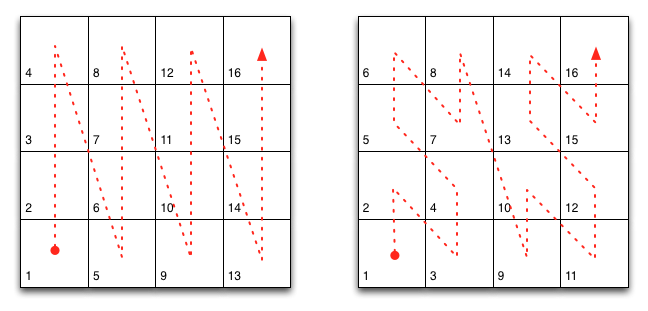
\includegraphics[width=0.65\textwidth]{rbffd_methods_content/neighbors/space_filling_curves.png}
\caption{Two example space filling curves to linearize the same fixed-grid. Left: Raster-ordering ($ijk$); Right: Morton-/Z-ordering.}
\label{fig:space_filling_curves}
\end{figure} 


At a high level, fixed-grid methods have the following construction steps \cite{Krog2010}:
\begin{enumerate}
\item Subdivide the domain with the overlay grid.
\item For each node, identify the containing cell coordinates (Equation~\ref{eq:cell_hash}).
\item For each node, use the cell coordinates as input to a spatial hash function (i.e., a space-filling curve).
\item Sort the nodes according to their spatial hash. 
\end{enumerate}
Particular details of how nodes are sorted, the choice of hashing function, the number of nodes allowed per cell, etc. determine the specific class of fixed-grid method and corresponding complexity. A comprehensive list of options and classifications can be found in \cite{Samet2005}. In this work multiple nodes with the same spatial hash retain their original relative ordering.

\subsection{Fixed-grid Construction}
The algorithm in this work is inspired by fixed-grid approaches for GPU particle simulations (\cite{Krog2010,Green2010,Johnson2011}). Particle methods require a ball query at each time-step. With time-steps often dominated by the cost of querying neighbors, the community understandably devotes significant effort to seek out the most efficient solutions possible \cite{Goswami2010}. The fixed-grid method is competitive for at least two reasons: a) by bypassing the need to build a tree, half the cost in querying neighbors is avoided; and b) nodes sorted according to a spatial hash reside closer in memory to nearby neighbors than in the case of unsorted nodes. The spatial locality moves stencil centers with shared nodes closer in memory, thereby improving the likelihood that data for the shared nodes will be resident in cache when it is required for reuse on consecutive stencil operations. 
Note that reordering by cell hash sorts nodes across cells but not within them---that is, nodes contained by the same cell are contiguous in memory, but remain arbitrarily ordered with respect one another. Fortunately, with contiguous groups of nodes, nearest neighbor queries can directly access all nodes per cell. 

Note that the fixed-grid method works best for quasi-uniform node distributions. In the case of non-uniform node distributions, the search cost is dominated by the regions of high node density.


The authors of \cite{Krog2010,Johnson2011,Green2010} assume a raster-ordering on cells, and that the uniform grid is sufficiently refined to ensure cells contain at most eight nodes. Particle interactions are limited to ball queries on the containing cell plus one halo of neighboring cells. The term \emph{halo} is used to describe the layer of cells neighboring a node's containing cell. The first halo refers to the 8 surrounding cells in 2-D and 26 cells in 3-D. The $i$-th halo in $d$-dimensions contains $\left(2(i+1)-1\right)^d - \left(2i - 1\right)^d$ cells. Returning to Figure~\ref{fig:nearest_neighbor_example}, we find two ball queries intersecting cells of of the first and second halos.


Since the number of cells to check is fixed, the neighboring nodes can be obtained by direct access in constant time. A similar approach is taken by \cite{Goswami2010}, but the authors opt for a $Z$-ordering of cells. 
 As a point of difference in implementations, the authors of \cite{Green2010, Krog2010, Goswami2010} leverage a fast radix sort algorithm to order nodes based on hash index, while \cite{Johnson2011} utilizes a slower bitonic sort algorithm. The fixed-grid method in \cite{Wendland2002,WendlandBook} forgoes logic to refine the grid and enforces a maximum limit on the number of nodes per cell. The author also avoids sorting nodes based on cell hashes. Instead, a list is maintained that stores the indices of all contained nodes per cell. %, which implies random memory access when operating on the nodes of a cell.    


The implementation presented here is a hybrid of the aforementioned algorithms. For example, cells are sorted based on raster-ordering, but without the restriction on a maximum number of nodes per cell. Rather than a radix- or bitonic sort to reorder nodes, the list of node indices for each cell (\cite{Wendland2002,WendlandBook}) is constructed as part of a single-pass bucket sort on the nodes. Finally, in stark contrast to  \cite{Krog2010,Green2010,Johnson2011,Wendland2002,WendlandBook}, querying neighbors is not restricted to a fixed radius, or number of cell halos. To satisfy the $k$-NN query, this implementation iteratively increases the query radius to include a new halo of cells at each iteration. This multi-pass ball-query was illustrated in Figure~\ref{fig:nearest_neighbor_example}. The iteration terminates when the desired count of neighboring nodes is satisfied or exceeded.
%TODO: Figure~\ref{fig:hash_highlevel} demonstrates the algorithm 
%\begin{figure}
%\centering
%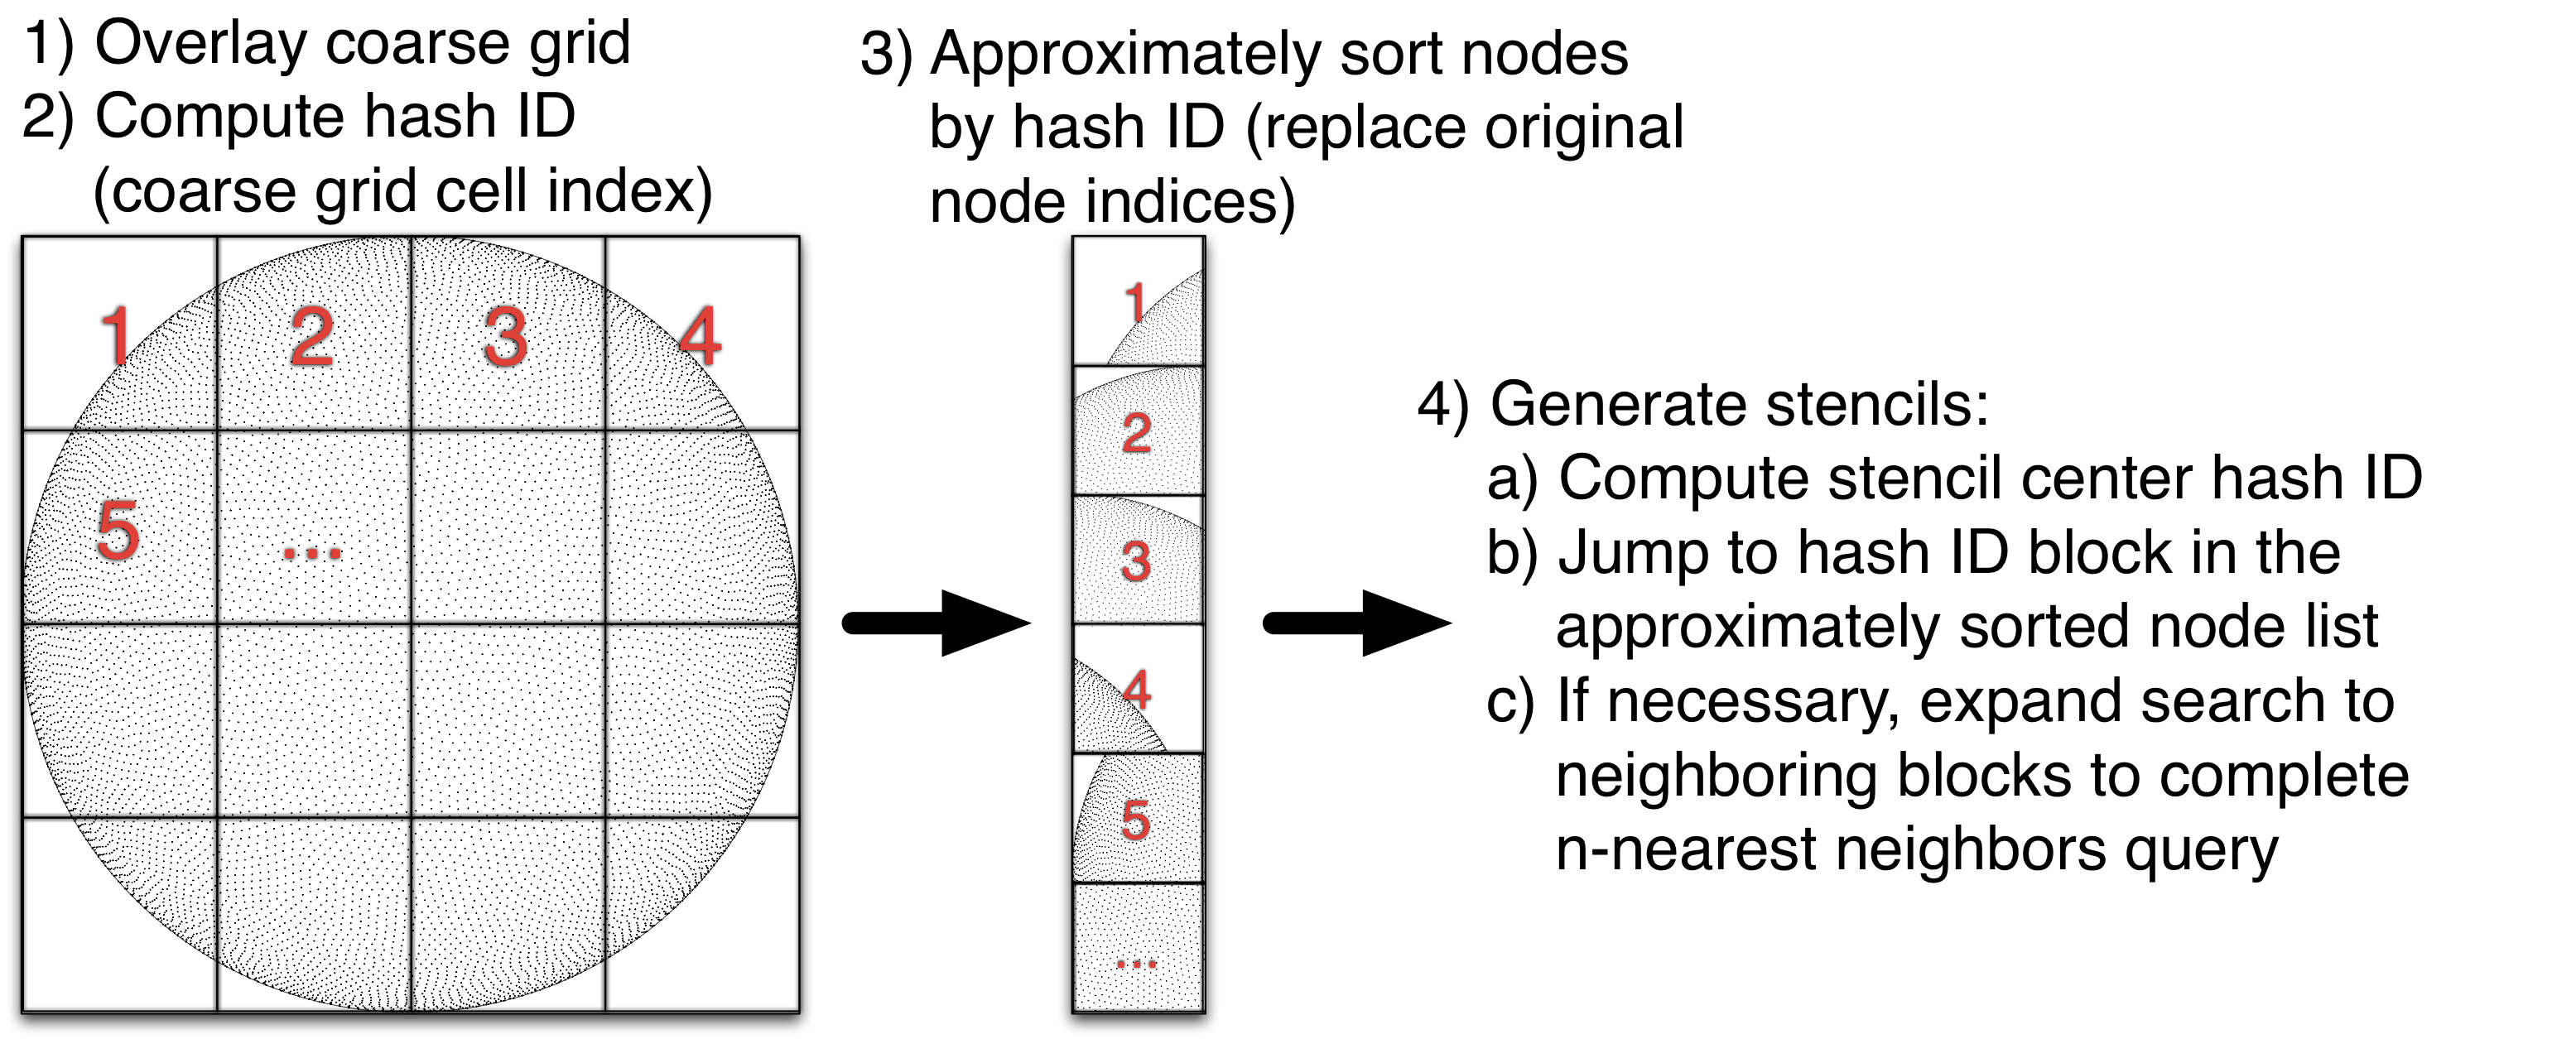
\includegraphics[width=1.0\textwidth]{../figures/chapter2/hashing_example/LSH_Concept.png}
%\caption{High level overview of the \emph{Fixed-Grid Bucket} (a.k.a. Hash) Algorithm. A coarse regular grid is overlaid on the domain. Nodes coordinates are hashed to containing cell indices and pushed onto a list for the appropriate cell. The cells are reordered in memory according to a space filling curve (i.e., Raster (IJK), Morton (Z), Graycode (U), etc.). Stencil queries start search with the cell containing the stencil center and expand to neighboring cells until at least $n$ candidate nodes are found. The candidate list is truncated to the $n$ closest neighbors. }
%\label{fig:hash_highlevel}
%\end{figure} 

\begin{algorithm} 
\caption{BuildFixedGrid($P$, $h_n$)}         
\label{alg:fixed_grid_build}  
\begin{algorithmic}[1]    
    \State \textbf{Input:} A set points $P$, and the fixed-grid resolution, $h_n$.
    \State \textbf{Output:} The reordered points in $P$, and corresponding cell buckets $Q$.
    \State
    \State Create $Q$: an $(h_n)^d$ array of empty buckets. 
    \For{point $p_i$ in $P$}
       \State $c := \text{CellCoords}(p_i)$ 
       \State $ind := \text{SpatialHash}(c)$
       \State Append index $i$ onto $Q[ind]$
    \EndFor
    \For{$j=0,1,...,(h_n)^d$}
    \If{$Q[j]$ is not empty}
        \State Append the set $P[Q[j]]$ onto $\hat{P}$
        \State Overwrite the set $Q[j]$ with new indices of $\hat{P}$ 
    \EndIf
    \EndFor
    \State $P := \hat{P}$
    \State \Return 
    \end{algorithmic}
\end{algorithm}

Algorithm~\ref{alg:fixed_grid_build} presents the fixed-grid build process. The routine starts by allocating an array of empty buckets, $Q$, which is populated based on the spatially hashed cell coordinates. The second for-loop in Algorithm~\ref{alg:fixed_grid_build} iterates through $Q$, looking for non-empty buckets. When one is found, nodes referenced by that bucket are transcribed/appended onto the ``sorted" list of nodes $\hat{P}$. This way the nodes in each cell are contiguous, but maintain the original ordering with respect to one another. Additionally, node indices in $\hat{P}$ replace the old indices within $Q$.

The entire build process complexity is proportional to $O(N)$, and requires $O((h_n)^d + N)$ storage. This approach as a \emph{fixed-grid bucket method with one-dimensional ordering} \cite{Samet2005}. The term \emph{bucket} refers to the allowance for each cell to contain an arbitrary number of nodes. \emph{One-dimensional ordering} is indicative of attempts later in the chapter to employ alternative space-filling curves in place of raster-ordering. 

A special note: rather than discarding the sorted nodes after stencil generation is complete, the final step of Algorithm~\ref{alg:fixed_grid_build} overwrites the original list of nodes with the sorted equivalent. This makes the sorted list available for reuse elsewhere. Since the first step in RBF-FD applications is to generate stencils, overwriting the input node set can guarantee that the node values throughout the entire life-cycle of an RBF-FD application will benefit from the same spatial locality as stencil generation. This benefit is (almost) free. 

Consider Figure~\ref{fig:reorder_example}, which shows two differentiation matrices generated based on the same $N=6400$ MD-node set (unit sphere), with each row representing an RBF-FD stencil of $n=50$ non-zeros (blue dots). The left matrix in Figure~\ref{fig:reorder_example} is generated with stencils queried by a $k$-D Tree. The $k$-D Tree maintains the original ordering on $P$. The matrix on the right of Figure~\ref{fig:reorder_example} is a permuted equivalent of the left, but results from a fixed-grid sorted by raster-ordering with a coarse grid resolution of $h_n = 10$. 

Looking at Figure~\ref{fig:reorder_example} it should be obvious that reordering the nodes can improve memory access patterns for SpMV. If each row is applied as a sparse dot-product with a dense vector, the more condensed non-zeros are in the row, the more likely values from the dense vector will be resident in cache when multiplying later rows. Likewise, non-zeros that appear on consecutive rows can benefit from cache reuse. Later in this chapter, the impact of spatial orderings are compared to determine how RBF-FD can benefit the most. 

\begin{figure}
\centering
\begin{subfigure}{0.425\textwidth}
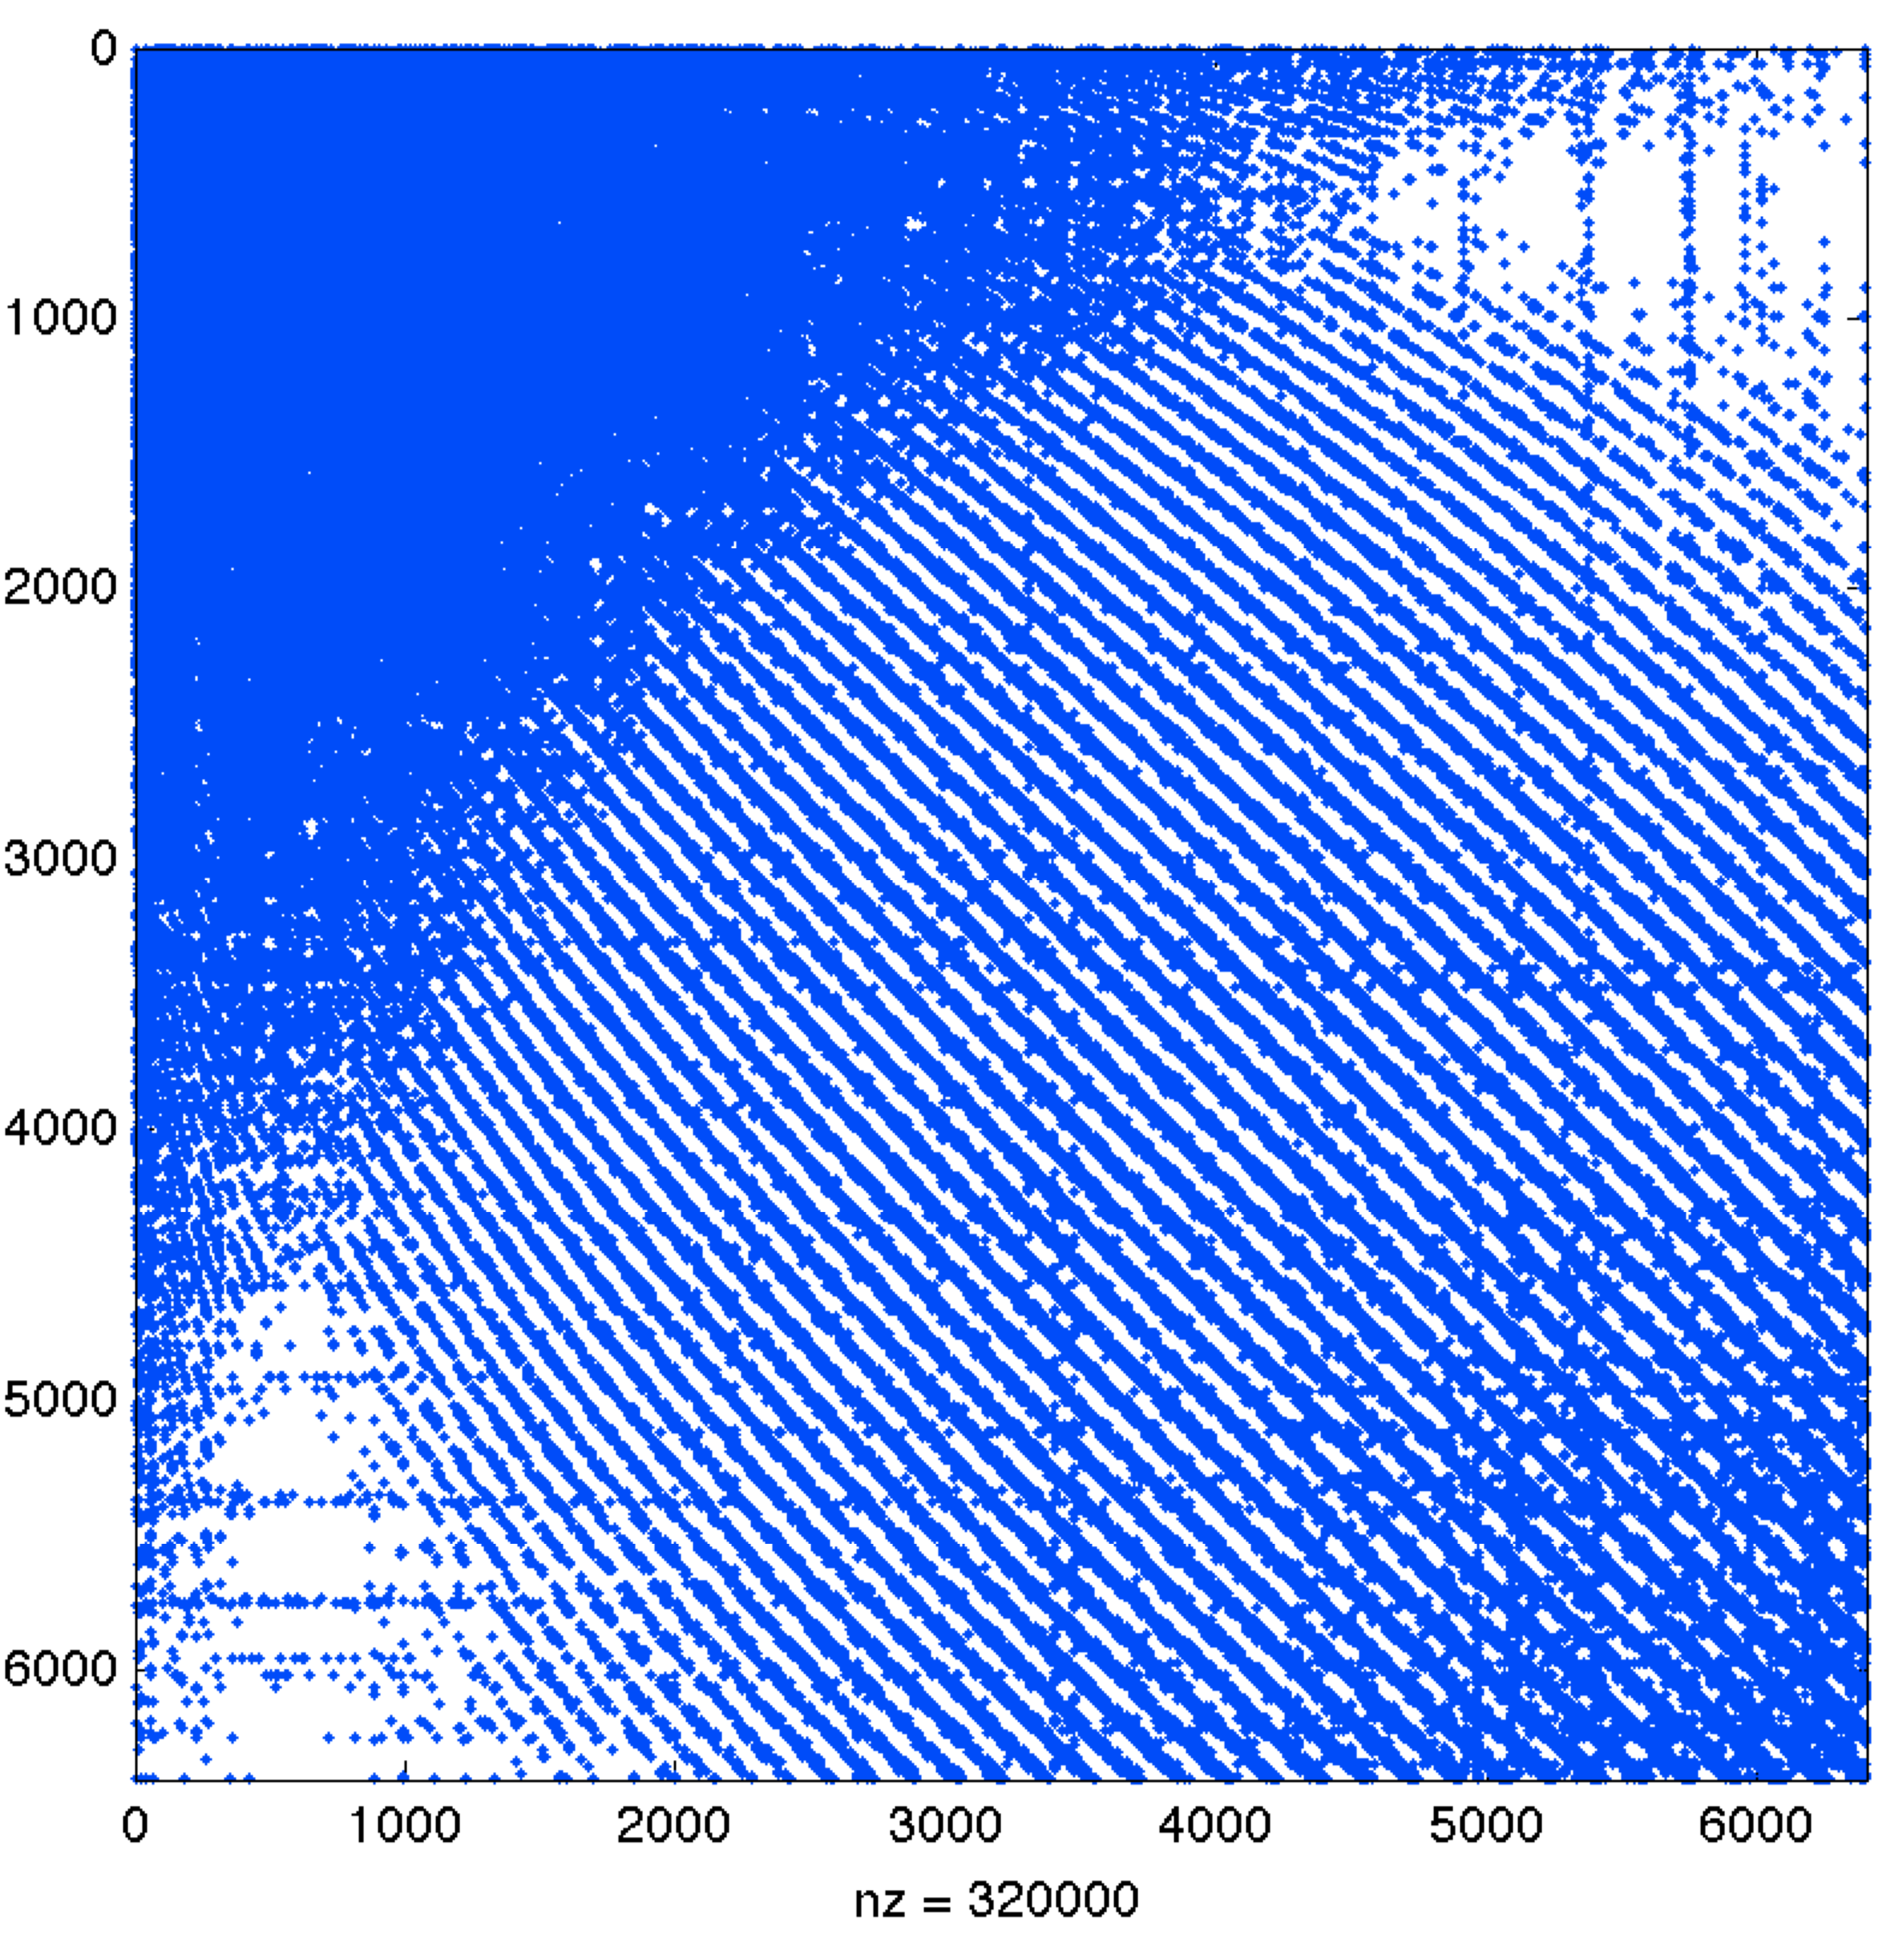
\includegraphics[width=1.0\textwidth]{../figures/chapter2/hashing_example/bruteforce_N6400_n50-eps-converted-to.png}
\caption{$k$-D Tree} 
\end{subfigure} 
\begin{subfigure}{0.425\textwidth}
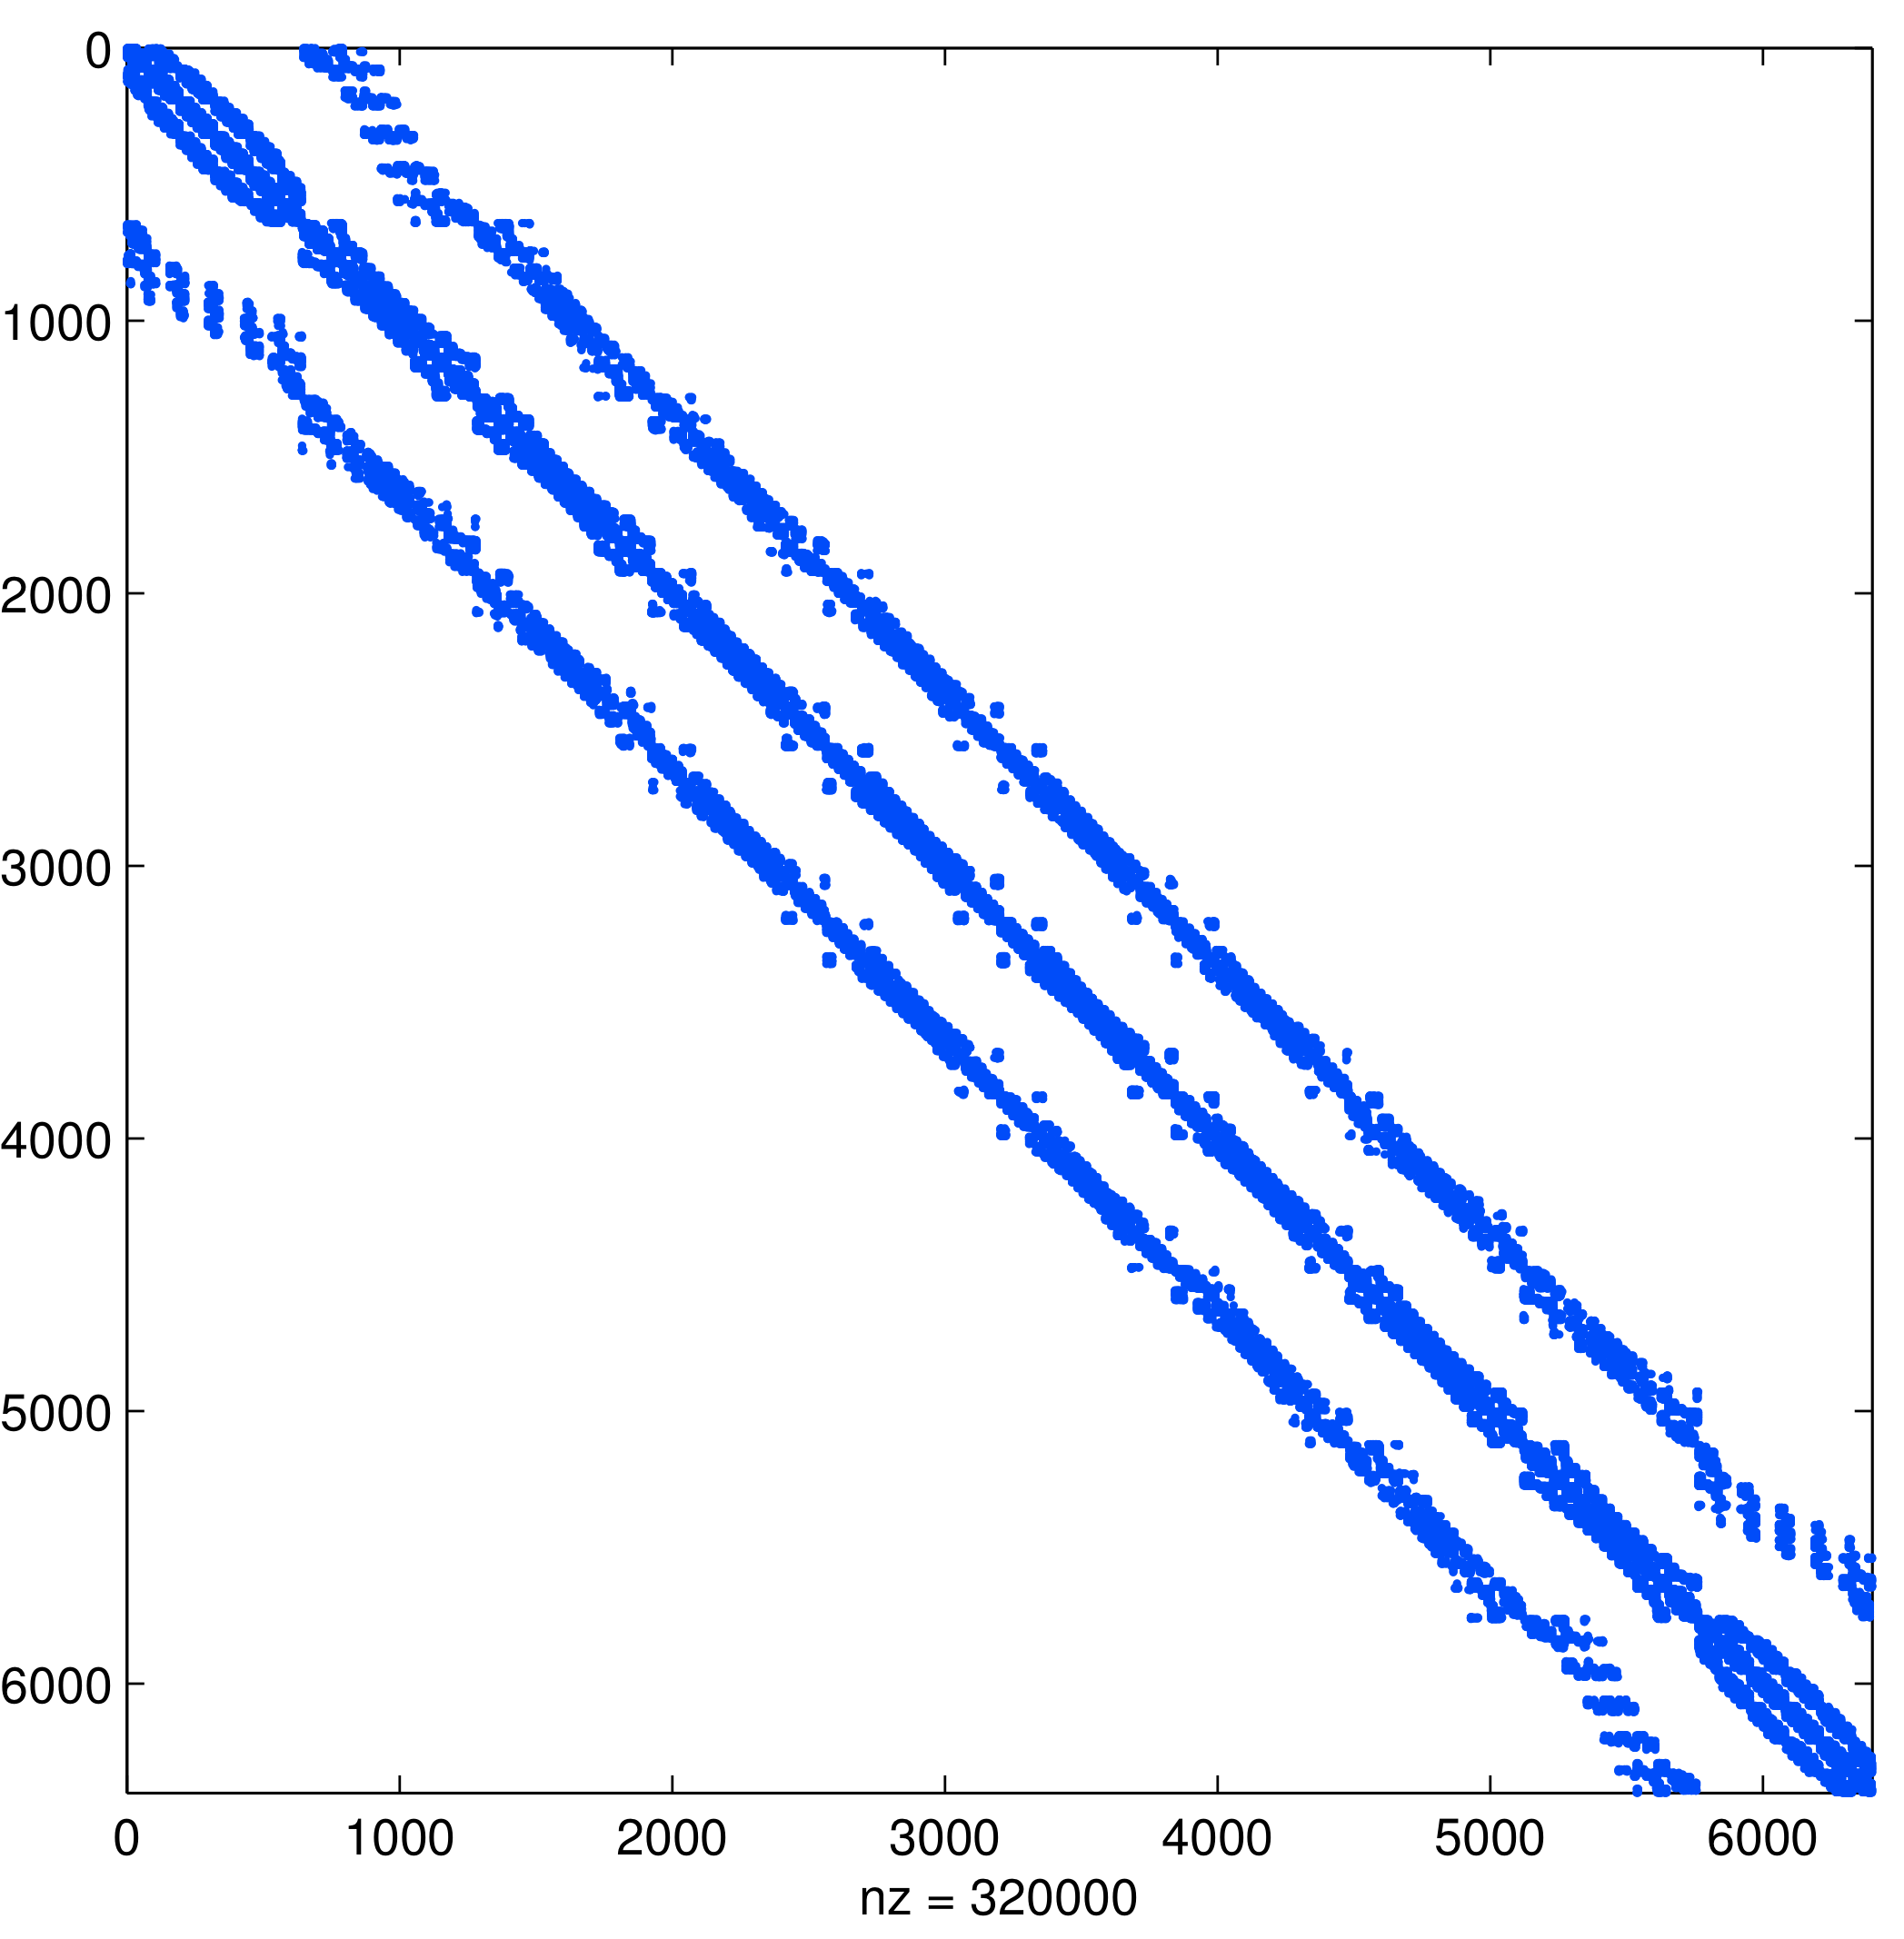
\includegraphics[width=1.0\textwidth]{../figures/chapter2/hashing_example/lsh_N6400_n50-eps-converted-to.png}
\caption{Fixed-Grid}
\end{subfigure}
\caption{Example effects of node reordering for MD node set $N=6400$ with $n=50$. The differentiation matrices are permuted equivalents and roughly $0.78\%$ full. Stencils generated based on $k$-D Tree maintain the original node ordering, while a fixed-grid with $h_n=10$ condenses non-zeros for improved memory access patterns (i.e., cache reuse).}
\label{fig:reorder_example}
\end{figure} 

\subsection{Fixed-Grid Neighbor Query}

Querying the $k$-nearest neighbors for a node, $X_q$, is the subject of Algorithm~\ref{alg:fixed_grid_query}. The process begins by finding $X_q$'s containing cell, $c$. The hash value of $c$ is used in Algorithm~\ref{alg:fixed_grid_query} to identify (in $Q$) the list of nodes contained within that cell, and then the identified nodes are appended to a list named $pq$, which accumulates all neighbor candidates. 

It is possible for the number nodes in $c$ to exceed $n$; however, the algorithm conservatively assumes that it is necessary to search at least one halo of cells around it.  This ensures that nodes near the cell boundaries will find nearby neighbors outside of the current cell, $c$, and the stencils will be balanced. Also, for certain fixed-grid resolutions, a single halo may not satisfy the stencil size requirements, so the algorithm iterates outward. As cells are checked, their nodes are appended to $pq$. 

The final stage of Algorithm~\ref{alg:fixed_grid_query} calculates the distance from all candidate nodes to $X_q$, and uses that metric to sort $pq$ in ascending order. The first $n$ nodes in $pq$ are returned as the stencil. 
\begin{algorithm} 
\caption{QueryFixedGrid($X_q$, $n$, $P$, $Q$ )}         
\label{alg:fixed_grid_query}  
\begin{algorithmic}[1]    
    \State \textbf{Input:} A query point, $X_q$; the desired number of neighbors, $n$; a set of $d$-dimensional points $P$; and the matching cell bucket list, $Q$.
    \State \textbf{Output:} The $n$-nearest neighbors list $pq$.
    \State     
    \State $halo := 1$
    \State $c := \text{CellCoords}(X_q)$ 
    \State $ind := \text{SpatialHash}(cells)$
    \State Append $P[Q[ind]]$ onto $pq$
    \While{$pq$.size $< n$ OR $halo < 2$}
        \State $cells := \text{NeighboringCellCoords}(c, halo)$
        \State $inds := \text{SpatialHash}(cells)$
        \For{each $q$ in $Q[inds]$}
            \If{$q$ is not empty} 
            \State Append node list $P[q]$ onto $pq$
            \EndIf
        \EndFor
        \State increment $halo$
    \EndWhile
    \State $dists := \text{ComputeDistances}(pq)$
    \State Sort $pq$ by $dists$
    \State \Return the first $n$ nodes in $pq$
    \end{algorithmic}
\end{algorithm}


The complexity of Algorithm~\ref{alg:fixed_grid_query} can vary based on the choice of $h_n$. For a sufficiently refined fixed-grid the $k$-ANN is dominated by the cost of the \emph{while-loop} is $O(\log h_n)$ operations per stencil. In the worst case, when $h_n$ is small, the cost of sorting $pq$ dominates, and is proportional to $O(N \log N)$ (using a C++ STL Sort).  
Results below demonstrate that proper choice of $h_n$ can maintain logarithmic complexity similar to the $k$-D Tree query. 


The fixed grid query algorithm is considered an \emph{approximate nearest neighbor} (ANN) search. Consider again the nodes in Figure~\ref{fig:nearest_neighbor_example}. A $k$-NN stencil of size $n=8$ should contain the blue center, all blue nodes, plus the red node and one black node. The true $k$-NN would select the black node in the right-most column of the grid (i.e. the node closer to the dashed ball query). Under the fixed-grid method, however, the alternate black node is selected even though it is more distant. This happens because the more distant black node occupies the second halo of cells around the stencil center, whereas the true near neighbor is in the third. Algorithm~\ref{alg:fixed_grid_query} is able to truncate the search in the second iteration by satisfying the requirement on $n$. 

%Similarly, if cells are rectangular in shape, the ball-query under fixed-grid functions as an ellipsoid. In this case, stencils are biased with more nodes in one direction. To combat this, and ensure spherical stencils, this work assumes the AABB bounding the domain is a cube (i.e., $d_x = d_y = d_z$). 

The difference between a true $k$-NN and $k$-ANN can be significant in terms of performance for the neighbor query, but has little or no impact on RBF-FD operation. The only differences in stencils between $k$-NN and $k$-ANN occur at stencil nodes furthest from the stencil center (i.e., nodes with the least impact on the stencil center). 


%\begin{figure}
%\centering
%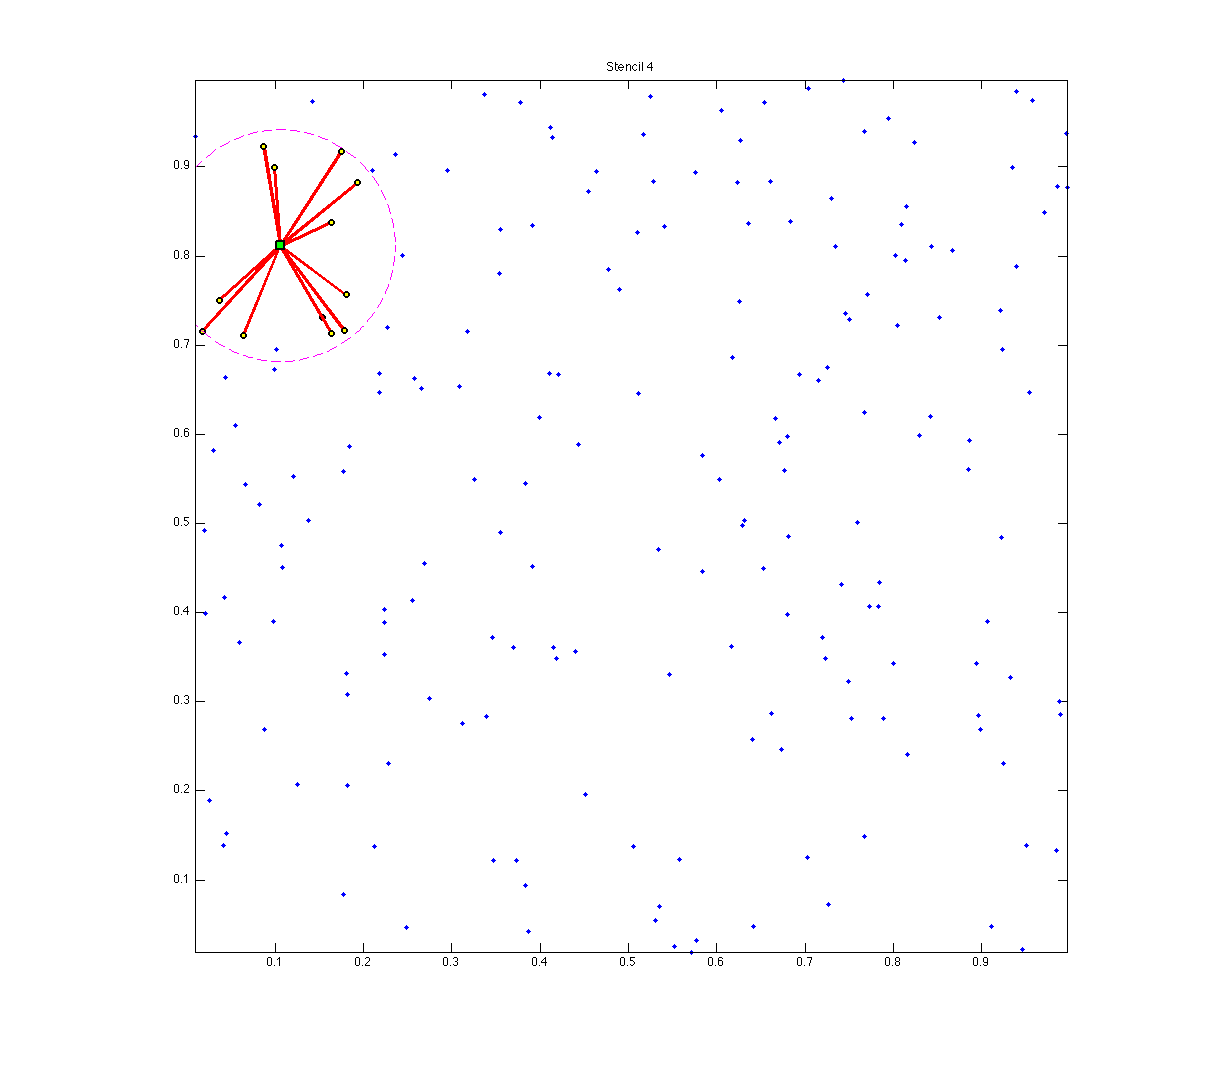
\includegraphics[width=8.5cm]{rbffd_methods_content/neighbors/neighbor_incorrect.png}
%\caption{A stencil generated with $k$-ANN satisfies the required stencil size, but is not guaranteed to choose the true nearest neighbors.}
%\label{fig:approximate_nearest_neighbors}
%\end{figure}


\section{Performance Comparison}
\label{sec:fixed_grid_benchmarks}

The implementation of $k$-D tree compared in this work, the \emph{$kd$-Tree Matlab} library, was originally posted to the Matlab FileExchange in 2008 \cite{TagliasacchiMFE} and now maintained as an independent Google Code project \cite{TagliasacchiGC}. The implementation is written in C++, but includes a MEX compiled interface, allowing for a consistent and efficient $k$-D Tree API in both languages. 
The original release of $kd$-Tree Matlab (pre-2012) was in use throughout the RBF community at the onset of this work. The dual language API is appealing for rapid-prototyping with MATLAB, and then porting applications to C++. 

The pre-2012 implementation of $kd$-Tree Matlab followed the $O(N \log N)$ expected complexity for neighbor queries, but cost significantly more to build the tree. While build times for small and medium sized grids (i.e., less than $N=50000$ nodes) were small enough to be inconspicuous, the implementation scaled as $O(N^2)$ making it prohibitively expensive for large problems. 

The high cost ultimately led to work on a fixed-grid method to test the concept of neighbor queries with low build costs. The original prototype developed in pure MATLAB (\cite{BolligRBFFixedGrid}), outperformed the ``efficient" MEX-compiled $k$-D Tree for problem sizes $N > 20000$, and lead to the development of a C++ implementation tested here. In the 2012 release of $kd$-Tree Matlab (\cite{TagliasacchiGC}), the author has significantly improved the performance of the build process to achieve the $O(N \log N)$ behavior expected for a Point $k$-D Tree with cyclic splitting as presented above. 

All benchmarks in this section were performed on the Itasca HPC cluster at the Minnesota Supercomputing Institute. Itasca is an HPLinux cluster with 1,134HP ProLiant blade servers, each with two-socket, quad-core 2.8 GHz Intel Xeon processors sharing at least 24GB of RAM \cite{MSIItasca}. Both $k$-D Tree and fixed-grid implementations are compiled with the Intel compiler toolchain (v13), and the ``-O3" optimizations for auto-vectorization, loop unrolling, etc.. 

Figure~\ref{fig:stencil_query_old_and_new} demonstrates the performance of the $k$-D Tree and the fixed-grid method on increasing 3-D regular grid resolutions up to four million nodes. Both the current $k$-D Tree implementation (2012) and the original implementation (pre-2012) are shown in Figure~\ref{fig:sten_query_a} as evidence of the significant improvement in the latest release. For comparison, the C++ fixed-grid method is shown with two resolutions: $h_n = 50$ and $h_n=100$. On the bottom, Figure~\ref{fig:stencil_query_old_and_new} shows the associated speedups---defined as the ratio of time to compute $k$-D Tree stencils, over the time for the same stencil generation with a fixed-grid---achieved over the more efficient release of $kd$-Tree Matlab. These results cover the total time to build the data-structure and query all stencils. The test grid is generated in raster-order, as is the fixed-grid. 


Prior to the 2012 improvements, the C++ implementation was over 130x faster for four million nodes. With the newer and more reasonable $k$-D Tree benchmarks, the fixed-grid method is only 2x faster in the best case shown here. Although 2x is not as impressive, it is a notable improvement. One issue in Figure~\ref{fig:stencil_query_old_and_new} is that the fixed-grid with $h_n=50$ is consistently more than twice as slow as the $k$-D Tree. This is due to under-resolved cells with 32 nodes per cell; $h_n=100$ has only 4 nodes per cell. For small $N$ the $k$-D Tree is faster than both resolutions of fixed grid due to over-resolution. As $N$ increases beyond one million nodes the $h_n=100$ fixed-grid loses ground on the $k$-D Tree due to under-resolution. 


\begin{figure}
\centering
\begin{subfigure}{11cm}
\centering
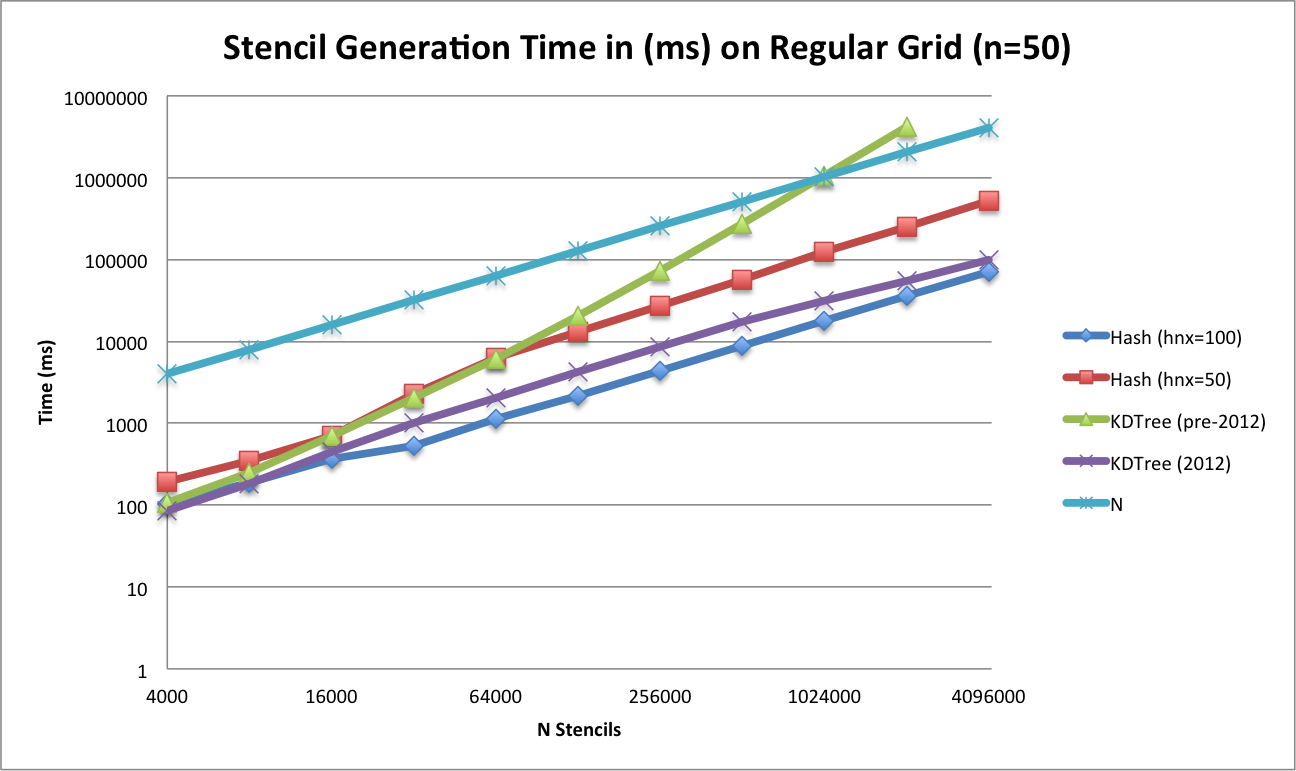
\includegraphics[width=\textwidth]{../figures/stencils/kdtree_old_reg_subsets_4m_stencil_gen_time.png}
\caption{3-D Regular Grid with stencil size $n=50$}
\label{fig:sten_query_a}
\end{subfigure}
\begin{subfigure}{9.5cm}
\centering
%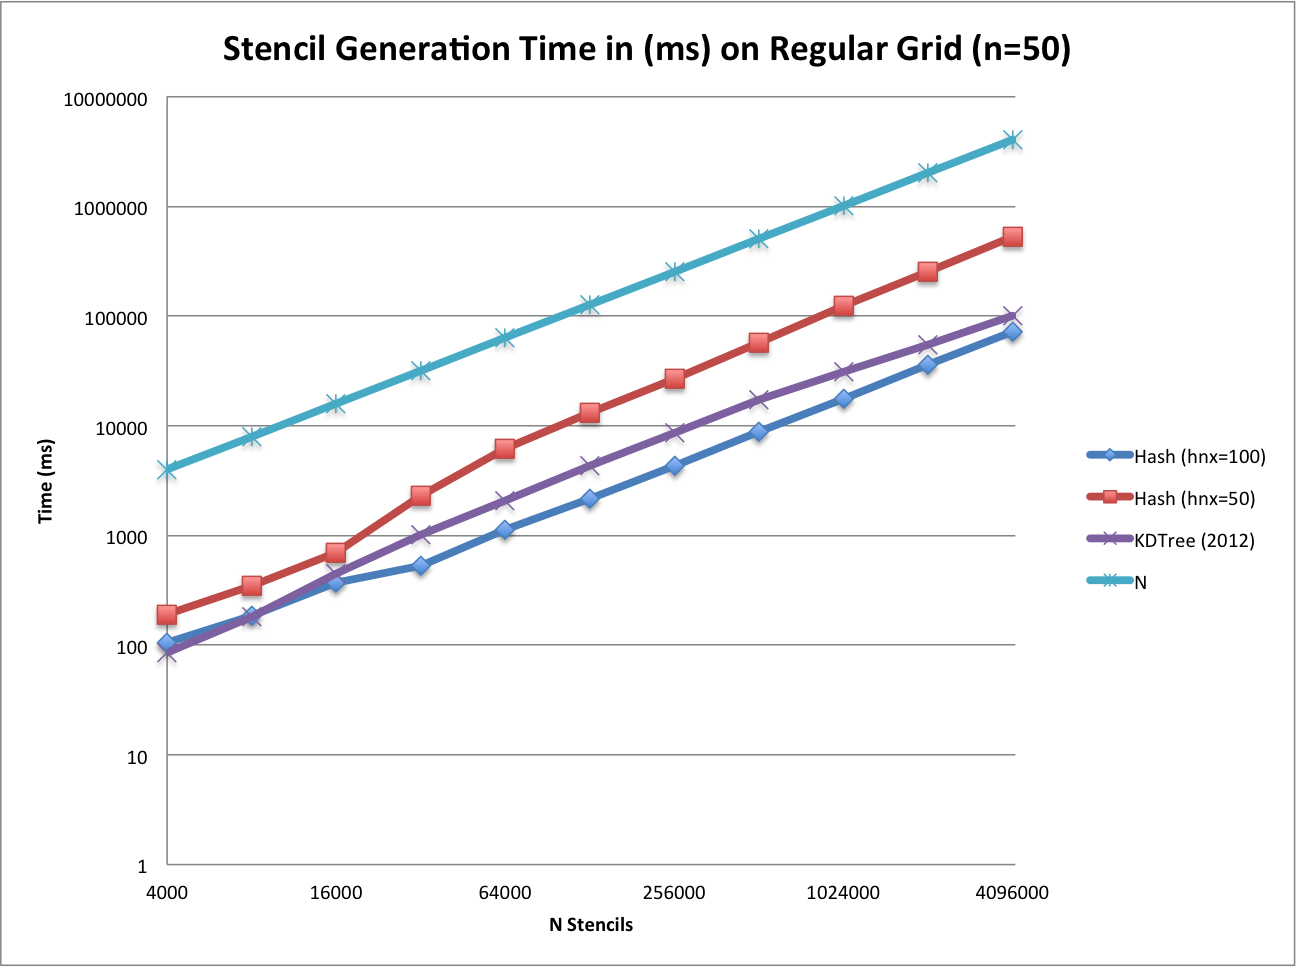
\includegraphics[width=9.5cm]{../figures/stencils/reg_subsets_4m_stencil_gen_time.png}
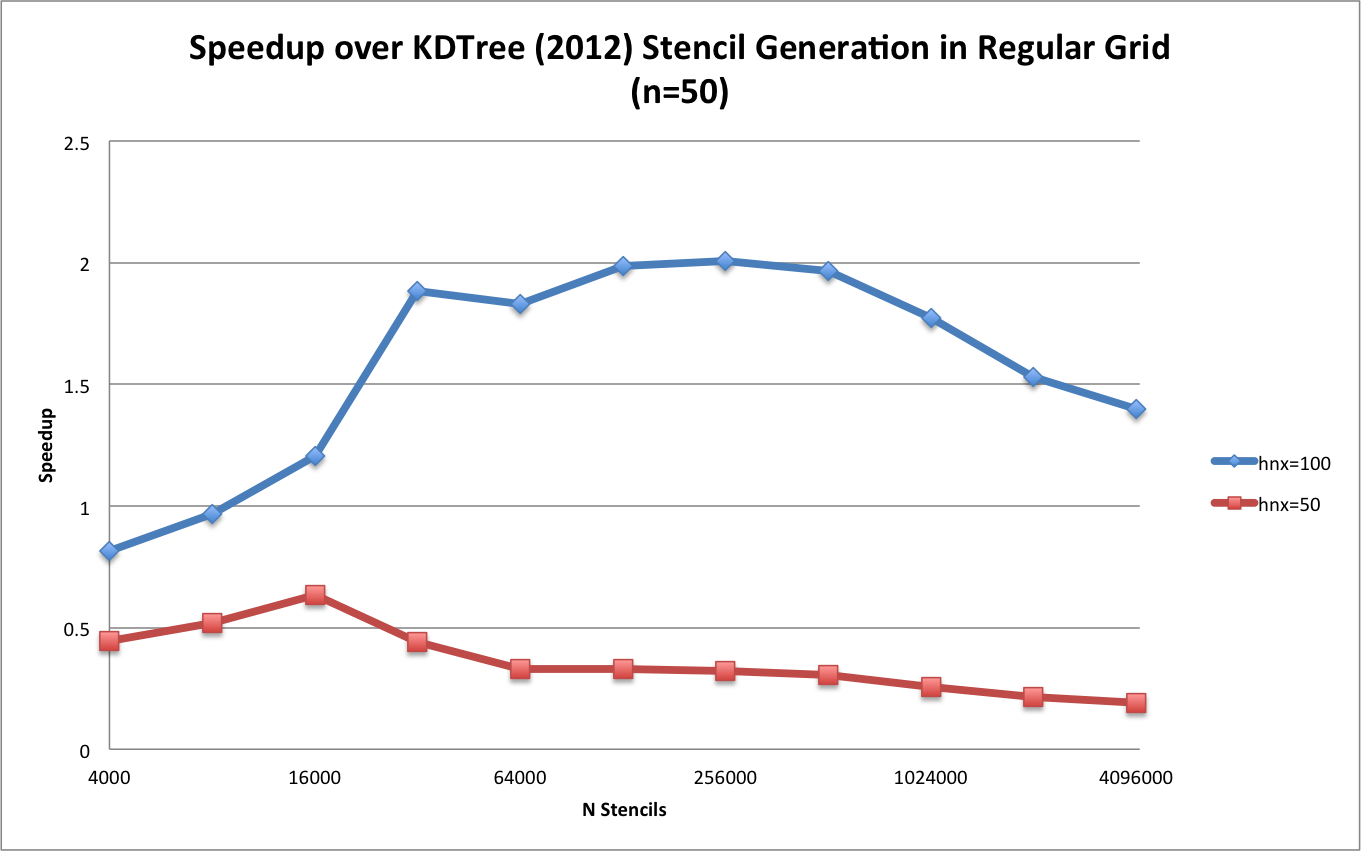
\includegraphics[width=\textwidth]{../figures/stencils/reg_subsets_4m_stencil_gen_speedup.png}
\caption{Speedup of fixed-grid method versus $k$-D Tree}
\end{subfigure}
%TODO: regenerate with true RG generated at specified resolutions
\caption{Querying the $n=50$ nearest neighbors on a regular grid up to $N=160^3$ demonstrates the gains achieved by the fixed-grid neighbor query method.}
\label{fig:stencil_query_old_and_new}
\end{figure}


Similar behavior is seen in Figure~\ref{fig:speedup_sphere} where the fixed-grid and $k$-D Tree are compared for various discretizations of the unit sphere. Each of the node sets described in Figure~\ref{fig:speedup_sphere} are discussed in Chapter~\ref{chap:rbffd_method} and available for download (\cite{BolligSphereGrids}). A range of resolutions are covered from a few hundred up to one million with some overlap. Each distribution (MD, Icosahedral, CVT) are generated differently and the nodes are naturally spatially sorted (icosahedral) or random (MD, CVT). Due to sorting in the fixed-grid method, node sets that are originally random exhibit more gain over $k$-D Tree. This is most evident in Figure~\ref{fig:speedup_sphere}, where different slopes appear for the segment corresponding to MD nodes and similar resolutions of Icosahedral nodes. The speedup curves for $h_n=50$ and $h_n=100$ demonstrate the dependence of fixed-grid method's success on the proper choice of $h_n$. When over-resolved (i.e., for $N < 10000$) the $k$-D Tree performs best. Under-resolution degrades performance rapidly starting at $N=100000$ for $h_n=50$, and $N=500000$ for $h_n=100$. 


\begin{figure}
\centering
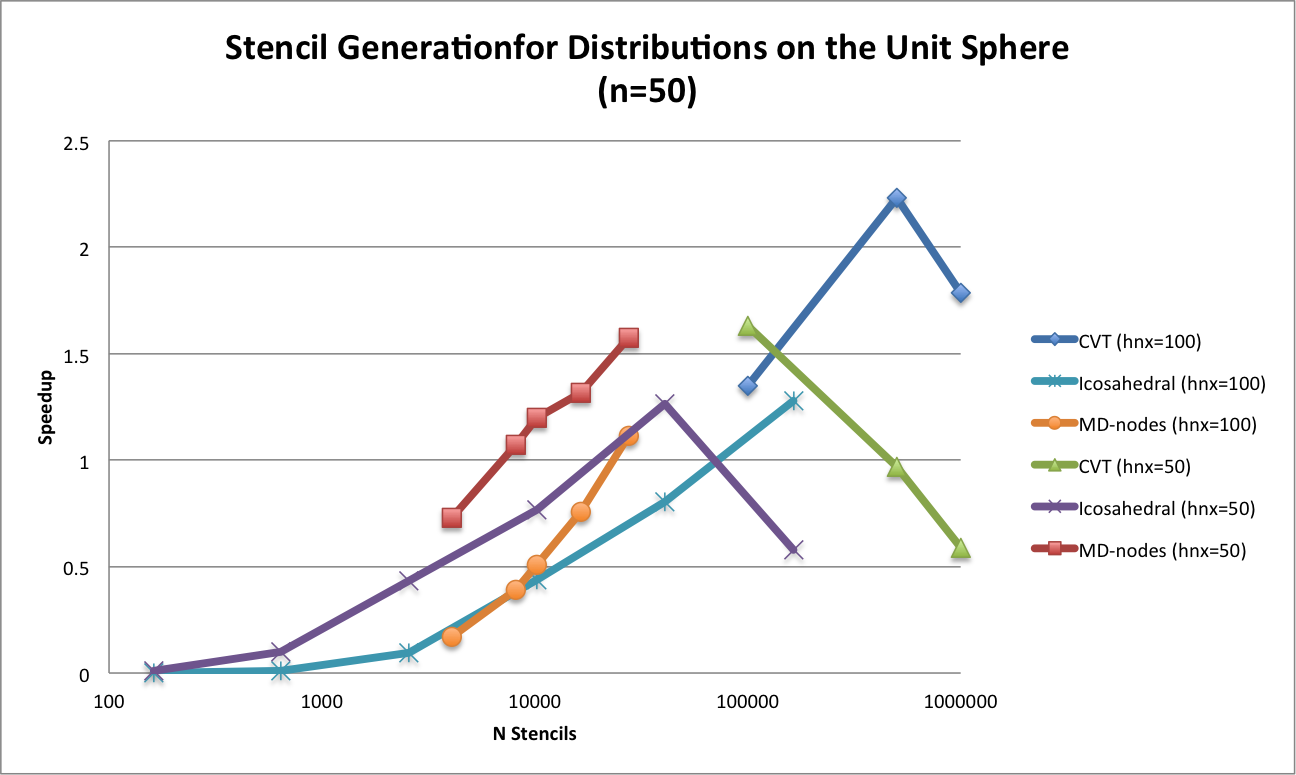
\includegraphics[width=10.5cm]{../figures/stencils/sphere_stencil_gen_speedup.png}
\caption{Fixed-grid speedup versus $k$-D Tree with stencil size $n=50$.}
\label{fig:speedup_sphere}
\end{figure}


The speedup curves in Figures~\ref{fig:stencil_query_old_and_new} and \ref{fig:speedup_sphere} hint at a maximum value $h_n$ for which the fixed-grid will outperform its competitor, and with that value: a maximum speedup possible. In Figure~\ref{fig:cvt_hn_speedup}, the $N=10^6$ resolution CVT is used to generate stencils of $n=50$, with range of values for $h_n$. The maximum of this curve shows that the fixed-grid can achieve up to 2.4x better than the $k$-D Tree for $h_n=160$. In this case the number of cells, $(h_n)^3$, sufficiently resolves the domain for most cells intersecting the sphere to have one or two nodes. At $h_n=70$ the fixed-grid is on par with $k$-D Tree; most cells have less than 8 nodes, which is consistent with the resolution sought by \cite{Krog2010,Goswami2010,Green2010}.

% NOTE: for 160^3 fixed grid for a CVT with 1-million nodes we have the following distribution: 
%  Count \mid Nodes Per Cell
%========================
% 3560709 0
% 409034 1
%  44542 2
%  13669 3
%  11480 4
%  11780 5
%  11422 6
%  10341 7
%   8518 8
%   6077 9
%   4037 10
%   2271 11
%   1190 12
%    552 13
%    243 14
%     86 15
%     38 16
%      9 17
%      1 19
%      1 20
%%%%%
%% Mean :               160            140        180         120            70
% exclude (0, 1, 2)	6.14186            
% exclude (0,1)	    4.68066          
% exclude (0)	        1.86814        2.02195     1.74984     2.24683        4.24401
% All	0.244141


\begin{figure}
\centering
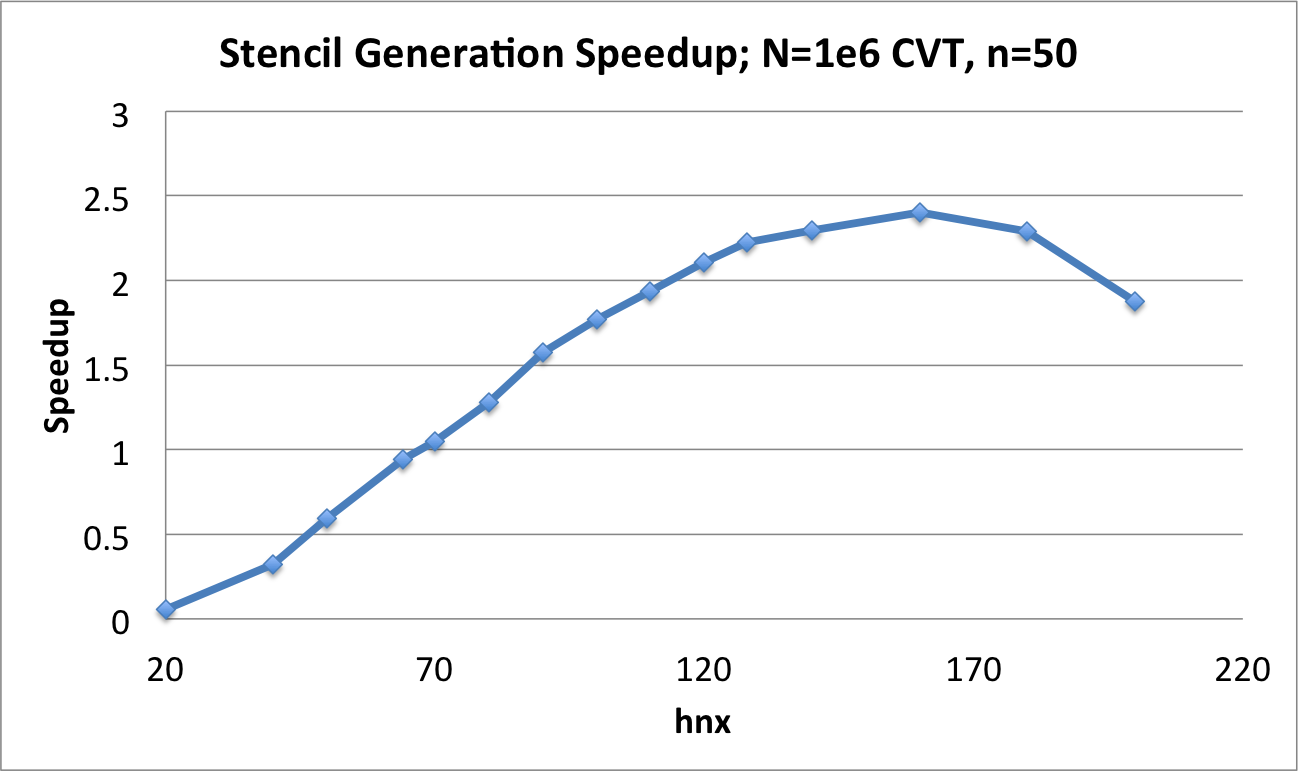
\includegraphics[width=9.5cm]{../figures/stencils/cvt1m_stencil_gen_speedup.png}
\caption{Fixed-grid speedup versus $k$-D Tree on a one-million node CVT (unit sphere), with stencil size $n=50$.}
\label{fig:cvt_hn_speedup}
\end{figure}

%TODO: repeat cvt_hn_speedup but get the number of nodes per cell.
\subsection{Impact on SpMV}

Based on evidence so far, the fixed-grid method is not a big winner against the $k$-D Tree, but it does eke out a small victory with the right choice of $h_n$. The reality is that stencil generation only occurs once, and the difference between $k$-D Tree and fixed-grid is easily amortized by iterations during the bulk of the RBF-FD application phase. However, as Figure~\ref{fig:spmv_impact_rg} illustrates, the fixed-grid method includes another longer lasting benefit. Namely, the Sparse Matrix-Vector Multiply (SpMV)---the major overhead in RBF-FD applications---benefits positively due to the reordering that occurs during stencil generation. Reordering cells improves locality of nearby nodes and associated values, and leads to up to 5x speedup in the SpMV for random node distributions. 

Regular grid and icosahedral sphere test cases in Figure~\ref{fig:spmv_impact_rg} see no more than 5\% improvement, which is unsurprising as their nodes are previously sorted. CVT and MD node sets, however, see a maximum speedup of 5x and 1.4x respectively. Furthermore, none of the test cases result in SpMV slowdown. Figure~\ref{fig:spmv_vs_hn} demonstrates the impact on SpMV as a function of $h_n$ for the $N=10^6$ CVT test case. The results show that even a coarse fixed-grid ($h_n \ge 40$) is capable of achieving the spatial locality of data that results in 5x faster SpMV. The combined results of 2x faster stencils and 5x faster SpMV make a case for the use of a fixed-grid query as a general safety net to precondition RBF-FD when properties of the input grid are unknown. 

\begin{figure}
\centering
\begin{subfigure}{9.5cm}
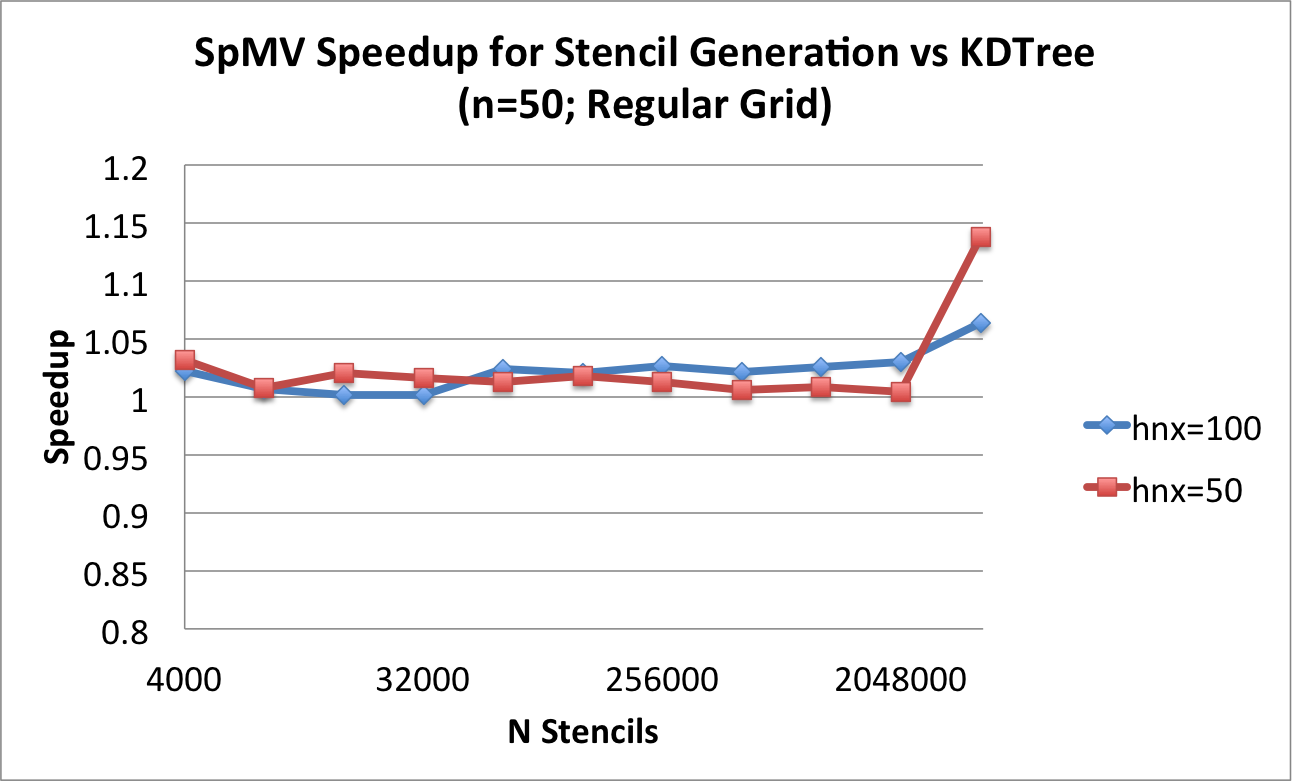
\includegraphics[width=\textwidth]{../figures/stencils/reg_subsets_4m_spmv_speedup.png}
\caption{3-D Regular Grid}
\end{subfigure}
\begin{subfigure}{10.5cm}
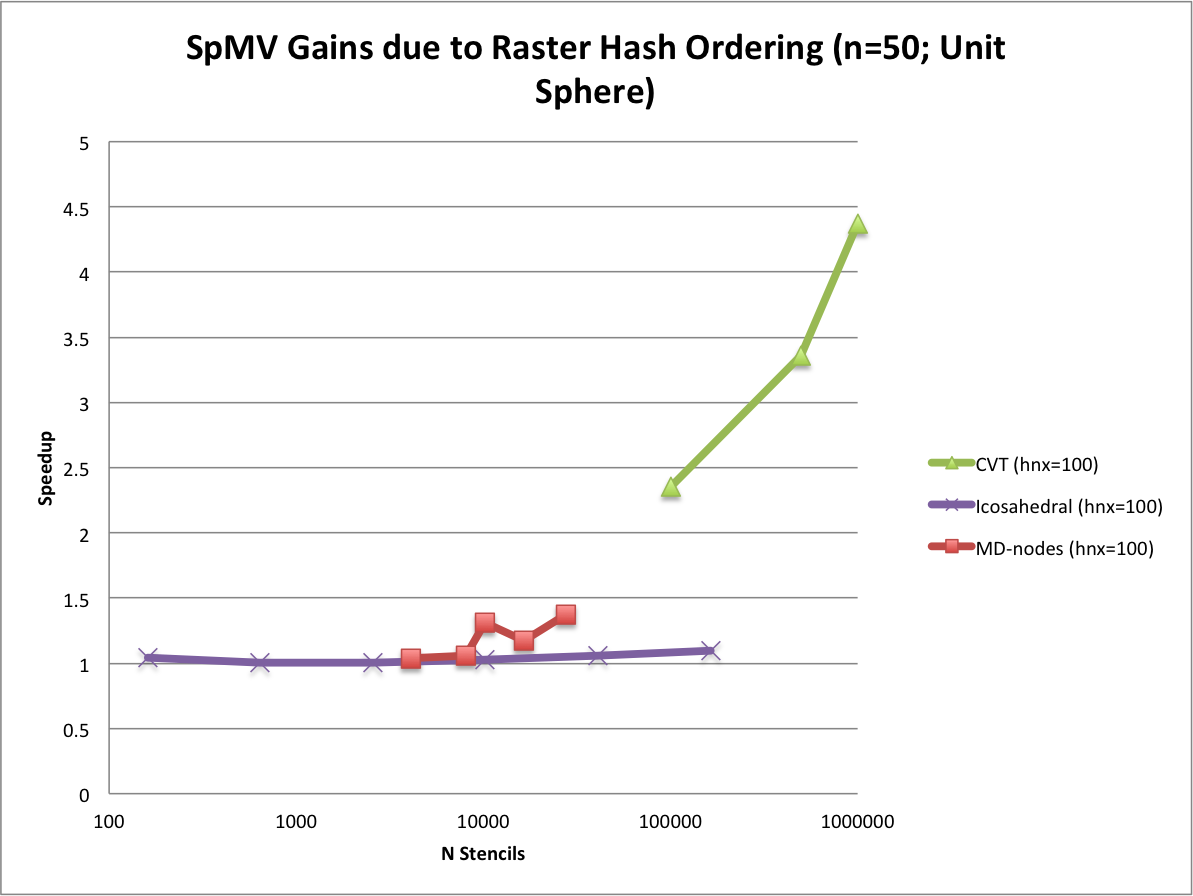
\includegraphics[width=\textwidth]{../figures/stencils/sphere_spmv_speedup.png} 
\caption{Unit Sphere}
\end{subfigure}
\caption{Fixed-grid impact on SpMV for stencil size $n=50$.}
\label{fig:spmv_impact_rg}
\end{figure}


%TODO: add function for N=1e5, 1e4 to see as a function of N and hnx. 
\begin{figure}
\centering
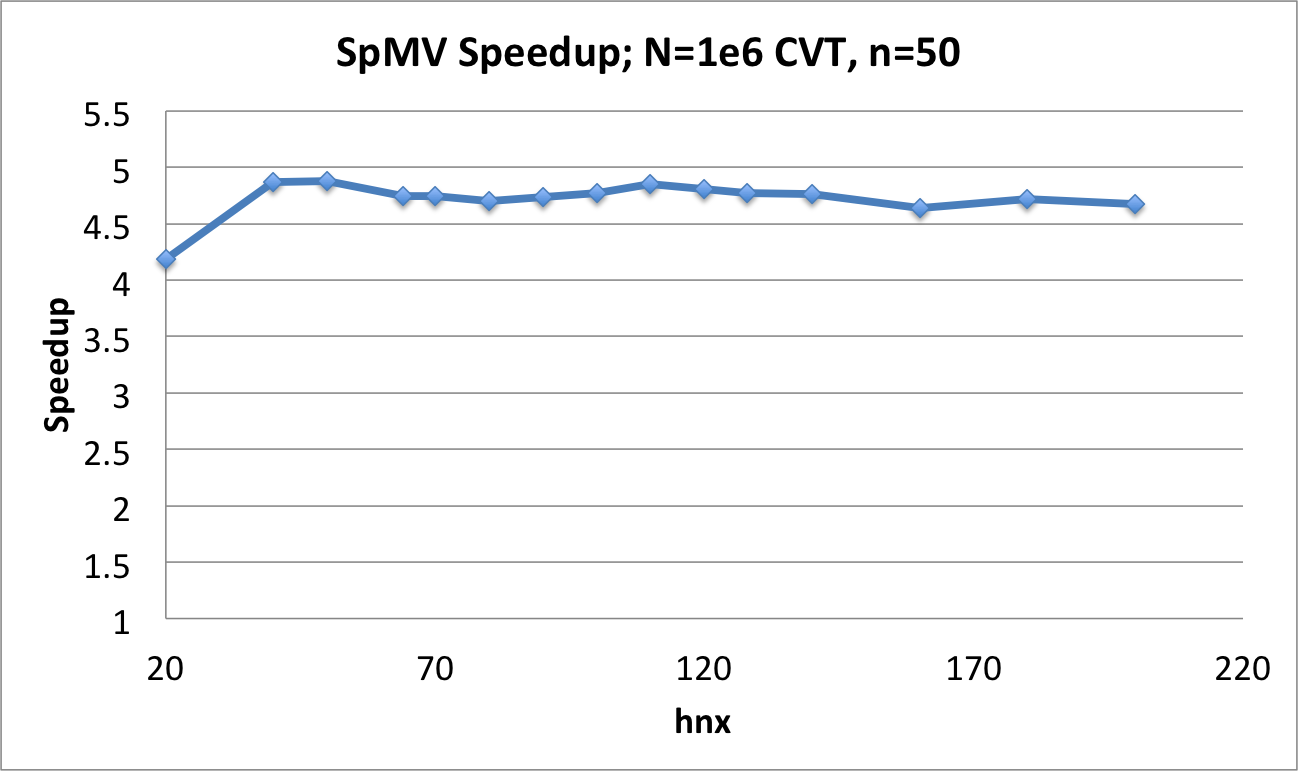
\includegraphics[width=7.5cm]{../figures/stencils/cvt1m_spmv_speedup.png} 
\caption{Impact on SpMV performance for $N=10^6$ CVT of the unit sphere due to choice of $h_n$.}
\label{fig:spmv_vs_hn}
\end{figure}


\section{Alternative Orderings}

As previously mentioned, the choice of space filling curve influences the sparsity pattern of differentiation matrices, which in turn impacts cache effects. The use of $Z$-ordering (Figure~\ref{fig:space_filling_curves}) for potential benefits on memory access is a common recommendation in fixed-grid methods (see e.g., the suggestions by \cite{Johnson2011,Green2010,Krog2010} and implementations in \cite{Goswami2010, MellorCrummey2001}). Under raster-ordering, cells are traversed with priority on one dimension. The resulting layout only has adjacent cells along that one dimension consecutive in memory. Other approaches, like $Z$-ordering, traverse cells by alternating dimensions/directions and increase locality of data in multiple dimensions. 

This section investigates the potential benefits of $Z$-ordering and various other space filling curves implemented as part of the original MATLAB fixed-grid prototype (\cite{BolligRBFFixedGrid}). Examples of the tested curves are presented in Figure~\ref{fig:orderings}. Here each node correlates to a fixed-grid cell, and curves start at coordinates $(0,0)$. 

Of the six cases shown in Figure~\ref{fig:orderings}, five of them (Raster, X, Z, U, 4-node Z) are directly produced via \emph{bit-interleaving} hash functions. Those same tiles are named based on the hierarchical pattern of connected nodes and groups of nodes. 

The sixth tile in Figure~\ref{fig:orderings} shows a Reverse Cuthill-McKee (RCM) ordering. The RCM method is distinct from the other orderings in that it is a \emph{bandwidth reduction} algorithm that focuses on condensing the sparsity pattern of differentiation matrices around the diagonal rather than spatially sorting nodes. Figure~\ref{fig:orderings} shows a special case that results when all nodes have stencils of size $n=3$. It nicely illustrates the RCM as a breadth-first traversal through the grid. More discussion on RCM occurs later in this section. 
\begin{figure}
\centering
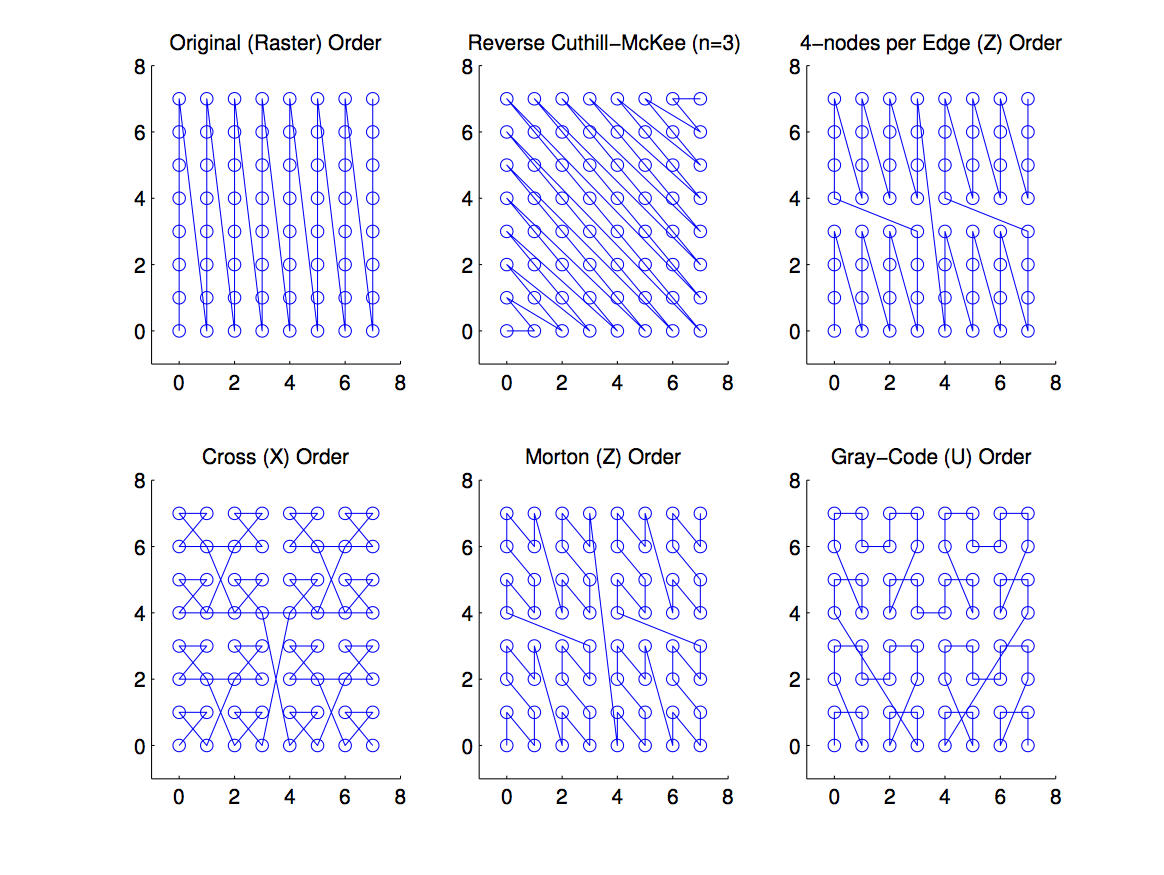
\includegraphics[width=0.9\textwidth]{rbffd_methods_content/hashing/node_orderings.png} 
\caption{Example space filling curves used to reorder cells/nodes. The Raster, $Z$-, $X$-, $U$- and 4-nodes per Edge $Z$-orderings are space filling curves applied to reorder cells of the fixed-grid stencil queries. Reverse Cuthill-McKee (RCM) operates on output stencils and their associated adjacency graph. The RCM shown here is a special case with only 3 neighbors per node.}
\label{fig:orderings}
\end{figure}

%TODO Investigations such as \cite{MellorCrummey2001} consider the impact of orderings on multiple levels of memory hierarchy

%TODO: ordering occurs when nodes are hashed to cell. Hash node with IJK, convert ijk to ordering, hash neighbors with IJK, convert ijk to ordering. Its a prototype, so performance of the conversion is not paramount. 
%TODO: why x, u, z, 4-node z? Originally it was Z, but the 


\subsection{Bit-Interleaved Orderings}

Bit-interleaving zips bits from two or more integers into one. For example, given two integers, $X$, and $Y$ the bits are interleaved as:
\begin{align}
X &= \{x_3x_2x_1x_0\} \nonumber \\
Y &= \{y_3y_2y_1y_0\} ,\nonumber \\
interleave(X,Y) & = \{x_3y_3x_2y_2x_1y_1x_0y_0\}. \label{eq:interleave_2d}
\end{align}
Including a third coordinate, $Z$, results in the following: 
\begin{align*}
interleave(X,Y,Z) & = \{x_3y_3z_3x_2y_2z_3x_1y_1z_3x_0y_0z_3\}.
\end{align*}

Interleaving depends on \emph{integer dilation} to modify an input integer value, so the output value has the original input bits spaced by new zeros. On a $d$-dimensional domain, bit-interleaving requires $d-1$ zeros between each bit. For example, dilating $1111_2$ expands the four bit integer to ${\color{red}0}1{\color{red}0}1{\color{red}0}1{\color{red}0}1_2$ in 2-D, and ${\color{red}0}{\color{red}0}1{\color{red}0}{\color{red}0}1{\color{red}0}{\color{red}0}1{\color{red}0}{\color{red}0}1_2$ in 3-D. 


The process to dilate integers applies multiple bit-mask operations to spread the digits appropriately. 
For any $b$-bit integer, $X_0$, the dilation is given by the following iteration:
\begin{align}
X_{i+1} = ((X_i \ll S_i) \mid X_i)\ \&\ M_i \ \ \ \ \ \text{for }i=0,...,\log_2(b)
\label{eq:dilate}
\end{align}
where operators $\ll$, $\mid$, and $\&$ indicate left-shift, bit-wise OR, and bit-wise AND operators respectively. In general, a $b$-bit integer requires $\log_2(b)$ iterations through the dilation kernel. The masks ($M_i$) and shifts ($S_i$) necessary to dilate a 32-bit integer are provided in Table~\ref{tbl:bitmasks2D} for 2-D, and Table~\ref{tbl:bitmasks3D} for 3-D. Both binary and hexadecimal representations are provided for $M_i$. Observe that the shifts and bit-masks applied during each iteration depend on the size of the integer and the dimension (refer to \cite{Stocco2009} for more details). 


\begin{table}
\centering
\caption{2-D Integer Dilation Masks for 32-Bit Integers}
\label{tbl:bitmasks2D}
\begin{tabular}{ c | c | c | c }
Level ($i$) & \multicolumn{2}{ c | }{Mask ($M_i$)} & $S_i$ \\ 
\hline
0 & $00000000000000001111111111111111_2$  & $0\text{x}0000ffff$  & 32 \\
1 & $11111111000000000000000011111111_2$  & $0\text{x}ff0000ff$  & 16 \\
2 & $00001111000000001111000000001111_2$  & $0\text{x}0f00f00f$  & 8 \\
3 & $11000011000011000011000011000011_2$  & $0\text{x}c30c30c3$  & 4 \\
4 & $01001001001001001001001001001001_2$  & $0\text{x}49249249$  & 2 \\
\hline
\end{tabular}
\end{table}

\begin{table}
\centering
\caption{3-D Integer Dilation Masks for 32-Bit Integers}
\label{tbl:bitmasks3D}
\begin{tabular}{ c | c | c | c }
Level ($i$) & \multicolumn{2}{ c | }{Mask ($M_i$)} & Shift ($S_i$) \\ 
\hline
0 & $00000000000000001111111111111111_2$  & $0\text{x}0000ffff$  & 48 \\
1 & $00000000000000000000000011111111_2$  & $0\text{x}000000ff$  & 24 \\
2 & $00000000000011110000000000001111_2$  & $0\text{x}000f000f$  & 12 \\
3 & $00000011000000110000001100000011_2$  & $0\text{x}03030303$  & 6 \\
4 & $00010001000100010001000100010001_2$  & $0\text{x}11111111$  & 3 \\
\hline
\end{tabular}
\end{table}


%At the end of Equation~\ref{eq:dilate}, the completely dilated integer is stored in $X_5$ with only one caveat: d
It is possible to lose bits in translation when dilating values that require greater than $\left\lfloor ^b/_d \right\rfloor$ bits. That means, in the case of 32-bits, any input to Equation~\ref{eq:dilate} must be representable in 16-bits or less (i.e., $X_0 \leq 65535 $) for 2-D, and 10-bits or less (i.e., $X_0 \leq 1023$) for 3-D. Note that these limits then become the maximum resolution possible for $h_n$ in the fixed-grid method. 

With dilation available, the process for 2-D bit-interleaving (Equation~\ref{eq:interleave_2d}) reduces to:
\begin{align}
(d_x, d_y) = (dilate(X), dilate(Y)) \nonumber \\
interleave(X,Y) = (d_x \ll 1) \mid d_y. 
\label{eq:interleave2d}
\end{align}
And in 3-D: 
\begin{align}
(d_x, d_y, d_z) = (dilate(X), dilate(Y), dilate(Z)) \nonumber \\
interleave(X,Y,Z) = ((d_x \ll 2) \mid (d_y \ll 1)) \mid d_z.
\label{eq:interleave3d}
\end{align}
Equations~\ref{eq:interleave2d} and \ref{eq:interleave3d} can be used as hash functions to produce a vast number of space filling curves (see \cite{Stocco2009}).

By default, Equation~\ref{eq:interleave2d} results in the $Z$-ordering in Figures~\ref{fig:space_filling_curves} and \ref{fig:orderings}. Consider for example:
\begin{align}
(c_x,c_y) & = (5, 3) = (0101_2, 0011_2) \nonumber \\
(d_x,d_y) & =  ({\color{red}0}0{\color{red}0}1{\color{red}0}0{\color{red}0}1_2, {\color{red}0}0{\color{red}0}0{\color{red}0}1{\color{red}0}1_2) \nonumber \\
interleave(c_x, c_y) & = ( 00100111_2 ) = 39. \nonumber
\end{align}
% 0000000100010
%  000000000101
% 0000000100111 = 32 + 7
The mapped $Z$-index of 39 can be verified by counting the number of steps from  $(0,0)$ to $(5,3)$ on the $Z$-order curve in Figure~\ref{fig:orderings}. 

The $X$- and $U$- orders shown in Figure~\ref{fig:orderings} also result from Equation~\ref{eq:interleave2d} with only slight modifications to the input. Table~\ref{tbl:orderings} provides a comparison of orderings and the operators/inputs in 2-D and 3-D that produce them. The $U$ and $X$ orderings depend on a bit-wise XOR operator, $\oplus$, to combine coordinates before interleaving. 

\begin{table}
\centering
\caption{Integer Dilation Interleaving Operators}
\label{tbl:orderings}
\begin{tabular}{ c | c | c }
  Ordering & 2-D & 3-D \\
  \hline                        
  IJK & $(X * h_n) + Y$ & $((X * h_n) + Y)*h_n + Z$ \\
  Z & $interleave(X, Y)$ & $interleave(X, Z, Y)$ \\
  U & $interleave(X, X \oplus Y)$ & $interleave(X, Z, Z \oplus Y)$ \\
  X & $interleave(X \oplus Y, X)$ & $interleave(X \oplus Y, Z, Y)$ \\
  4-Node Z * & $(d_x \ll 2) \mid d_y$ & $((d_x \ll 4) \mid (d_z \ll 2)) \mid d_y$ \\
  \hline  
\end{tabular}
\end{table}


The last row of Table~\ref{tbl:orderings}, the 4-node $Z$-curve, is a special case of bit interleaving. The 4-node Z is similar in theory to a standard $Z$-order, except that an extra zero per bit is requested when coordinates are dilated as though the process were operating in the next higher dimension. Then, using the operators provided in Table~\ref{tbl:orderings} to interleave bits results in the following pattern:
\begin{align*}
interleave_{4node}(X,Y) = \{x_5x_4y_5y_4x_3x_2y_3y_2x_1x_0y_1y_0\}.
\end{align*}
By reserving two bits for each dimension, the 4-node $Z$-curve is able to traverse up to four nodes in the $Y$ direction before taking its first step in the $X$ direction. 

%TODO: why was each curve chosen? 
% Z because of others like Goswami; U because it also widely used (gray-code)


Often, interleaved cell coordinates near the boundaries of the domain do not produce contiguous hash indices and may balloon to values greater than the number of nodes/cells in the domain. In these situations, missing indices reference coordinates outside the domain that would complete the hierarchical power-of-2 curves before entering the domain again. When sorted and traversed least to greatest, the hashed indices give a proper ordering of the domain, and missing indices are skipped. 

%TODO: how are reorderings applied


\subsection{Bandwidth Reduction and Reverse Cuthill-McKee} 

The purpose of reordering nodes/cells is to improve memory access patterns. If condensing non-zeros of a sparse matrix achieves this, then the ideal case arises when $n$ non-zeros occupy the first $n$ diagonals of the matrix (including the main diagonal) for all rows. In terms of stencils on a grid, this ideal case corresponds to all nodes on a 1-D line connected to their left and right nearest neighbors. In higher dimensions, reproducing the ideal structure requires one to neglect spatially nearest neighbors, except in cases of very low resolution or small stencil sizes, and select neighbors by following a space filling curve left and right. Stencils in 2-D or 3-D constructed through $k$-NN (or $k$-ANN) queries result in a sparsity pattern with gaps between non-zeros. In the worst case, matrices would have non-zeros in each row spaced as far apart as possible while maintaining the appropriate connectedness of the adjacency graph. 


As a measure of how well condensed non-zeros are, the \emph{bandwidth} of a matrix, $A$, is defined as (\cite{Cuthill1969, LiuSherman1976}): 
\begin{align*}
bw(A) = \max\{|i - j| + 1 : A_{i,j} \neq 0\}.
\end{align*}
The bandwidth simply counts the number of super- and sub-diagonals---i.e., diagonals above and below the main diagonal---that contain at least one non-zero. Incrementing by one accounts for a non-zero main diagonal. The lower the bandwidth, the better. 

For any matrix, $A$, a permutation, $P$, can be constructed such that 
\begin{align*}
P A P^T
\end{align*}
reorders the matrix and reduces the bandwidth of $A$. A variety of \emph{bandwidth reduction} algorithms exist with unique approaches for the construction of $P$ (see e.g., \cite{Gibbs1976, LiuSherman1976, MellorCrummey2001}).  In contrast to the space filling curves discussed above, bandwidth reduction algorithms are applied \emph{after} stencils are generated in order to operate on the differentiation matrix and corresponding adjacency graph. 

The effect pre- and post-multiplying $A$ by $P$ is equivalent to reindexing nodes and and updating all stencil connections to the new numbering. In practice, rather than construct a full permutation matrix $P$, which has exactly one 1 per row and per column, it is common to represent $P$ as a vector where each entry indicates the column location of the 1. In that case the vector elements reference the original node ordering, and the indices of those elements provide the new ordering. 

The most popular methods for bandwidth reduction are Cuthill-McKee (CM) algorithms \cite{Cuthill1969, LiuSherman1976}. In particular this work is concerned with the \emph{Reverse Cuthill-McKee} (RCM) variant. The authors of \cite{LiuSherman1976} show that, in comparison to regular CM, the RCM algorithm offers better conditioning of $PAP^T$ for reduced fill-in and reduced computation during matrix decompositions. Although fill-in is not a concern in this work, the RCM variant is attained at no extra cost.

At a high level, CM methods start by selecting a node in the adjacency graph with the lowest degree (i.e., fewest non-zeros per row in the matrix). From that node, a breadth-first traversal begins, passing through all connected neighbors in order from least to greatest degree. If nodes have the same degree, as is the situation for RBF-FD with stencil size, $n$, then ties are broken arbitrarily. The original indices for visited nodes are pushed onto a queue, $r$. Another queue is maintained to catalogue previously traversed nodes and prevent the process from doubling back on itself. In the event that the adjacency graph has multiple disconnected sub-graphs, the algorithm exhausts the first sub-graph before beginning the next; as always, beginning with the lowest degree node available. 

CM methods produce $r$ as the vector representation of $P$. The RCM variant differs from CM by reversing the order of $r$ so that rows corresponding to the last traversed nodes are at the top of $PAP^T$. 

Most CM and RCM implementations assume the algorithms operate on square, symmetric adjacency matrices. In the case of RBF-FD the adjacency matrices are symmetrized with $A+A^T$. For rectangular matrices with dimensions $N \times M$ (as are encountered in Chapter~\ref{chap:distributed_rbffd}), RCM is applied only to the $N\times N$ square block with symmetry similarly constructed. 


%Figure~\ref{fig:rcm_example} provides an example of RCM bandwidth reduction for the adjacency graph produced by $N=8^2$ nodes, each with a stencil of size $n=5$ (320 non-zeros). The grid of nodes is originally raster-ordered. In Figure~\ref{fig:rcm_dm_before_after} the matrix before and after RCM is shown with the bandwidth, $bw$, included in the $x$-label. 
%
%\begin{figure}
%\centering
%\begin{subfigure}{12.5cm}
%\centering
%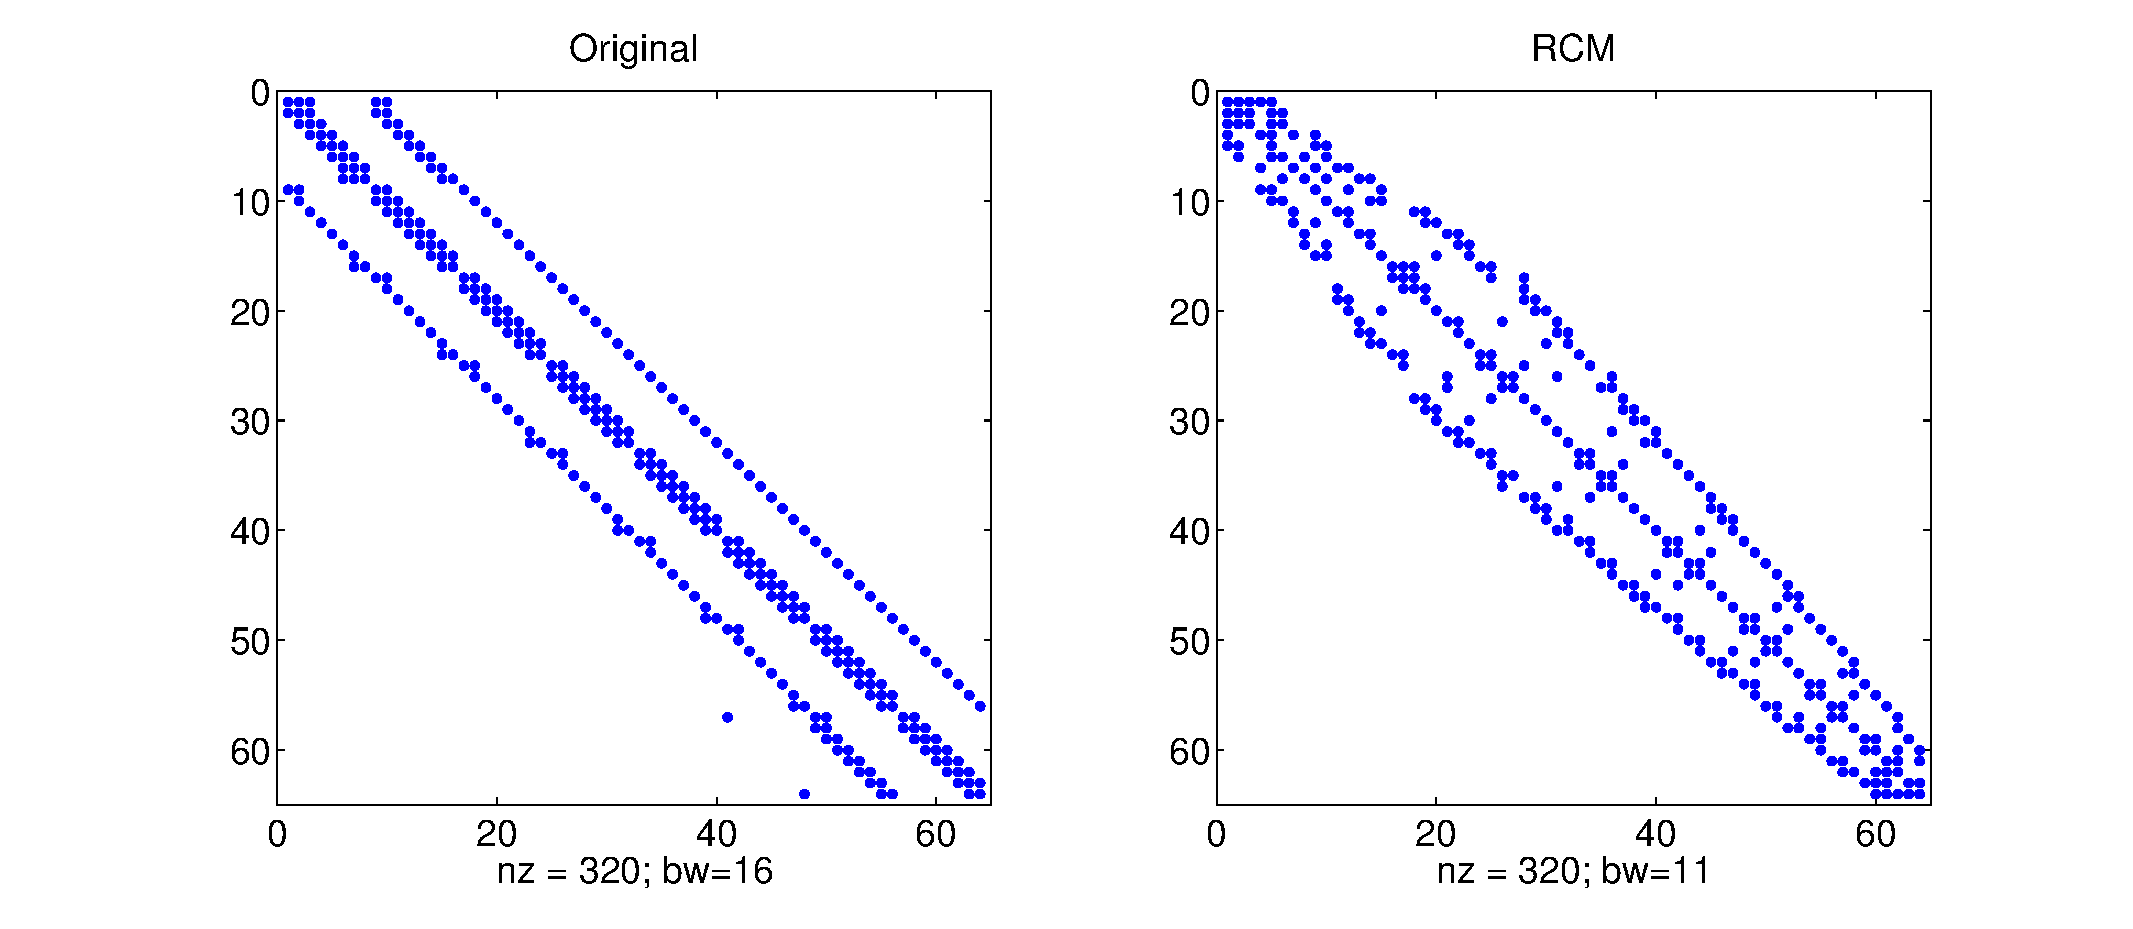
\includegraphics[width=\textwidth]{rbffd_methods_content/hashing/rcm_example_dm-eps-converted-to.pdf} 
%\label{fig:rcm_dm_before_after}
%\caption{DM before and after}
%\end{subfigure}
%\begin{subfigure}{12.5cm}
%\centering
%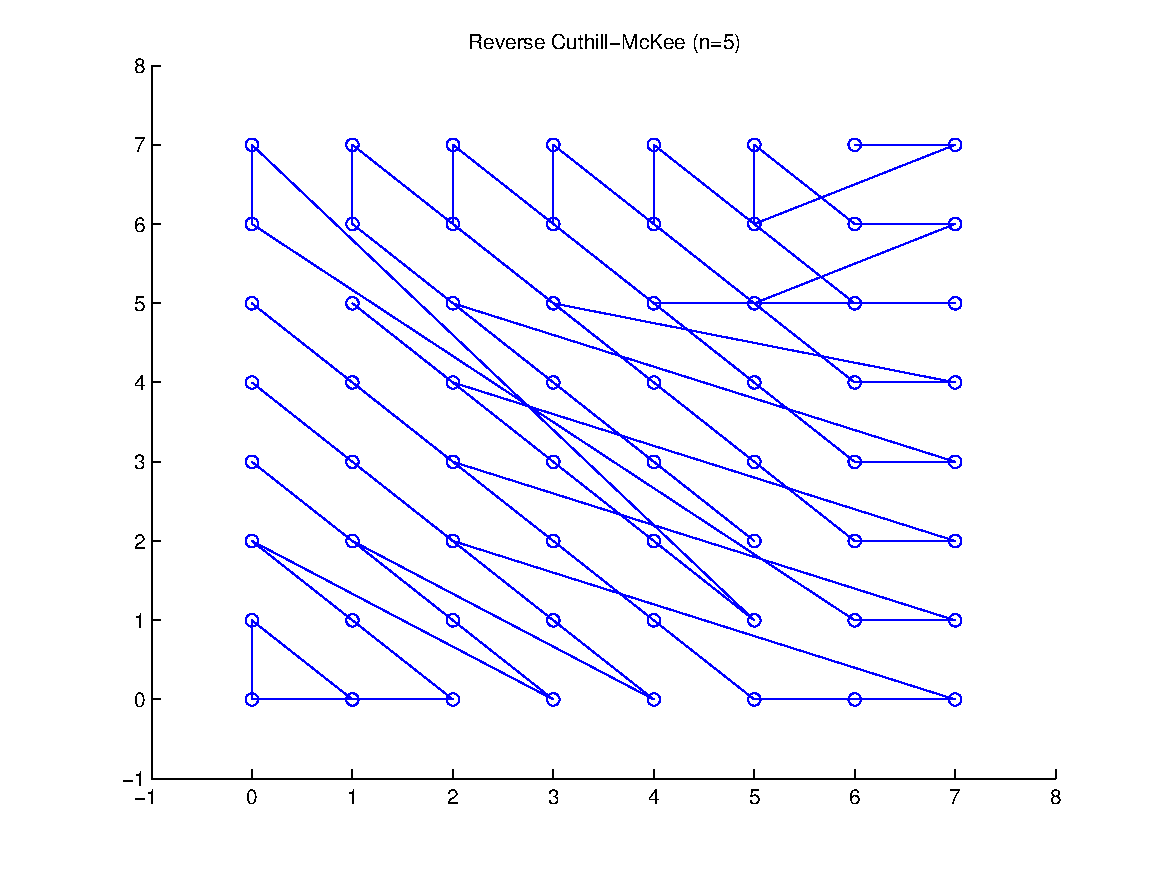
\includegraphics[width=\textwidth]{rbffd_methods_content/hashing/node_ordering_rcm_n5-eps-converted-to.pdf} 
%\caption{The RCM Ordering Curve}
%\label{fig:rcm_curve}
%\end{subfigure}
%\caption{An RCM reordering of $N=64$ nodes with stencil size $n=5$.}
%\label{fig:rcm_example}
%\end{figure}



%TODO: metric; mean speedup in SpMV for range of orderings based on optimal h_n per grid resolution. 
%TODO: metric; ideal h_n per grid resolution; sphere. 

\subsection{Impact of Orderings}

To compare the impact of orderings in Figure~\ref{fig:orderings}, the MATLAB implementation of fixed-grid (\cite{BolligRBFFixedGrid}) generates stencils and writes the sorted nodes and stencils to disk. The nodes and stencils are accepted as input for the C++ SpMV benchmark used above to compare 
the $k$-D Tree and fixed-grid stencils. Visualization and bandwidth calculation are both managed in MATLAB. 
Bit interleaving occurs in a MATLAB script that leverages the internal \emph{bitshift}, \emph{bitand}, \emph{bitor}, and \emph{bitxor} routines for bitwise operations. Bitwise operators in MATLAB are restricted to 32-bits, but the maximum number of cells per dimension allowed by 32-bits ($\leq 1023$ in $3$-D) is more than sufficient. The MATLAB internal \emph{symrcm} computes the Reverse Cuthill-McKee reordering. % based on the output from the raster-order (IJK) stencil generation. 
Since the same number of non-zeros exist per row, RCM selects a different starting node based on the input ordering of nodes; this allows for some variance in the bandwidth. For consistency, results shown here apply RCM to the output of a raster-ordered fixed-grid query. 

Figure~\ref{fig:ordering_impact_rg} illustrates six sparsity patterns resulting from the curves in Figure~\ref{fig:orderings}. The test case is a regular grid of $N=18^3$ nodes, each with stencil size $n=31$. From left to right, the top row shows raster-ordering, Reverse Cuthill-McKee, and the 4-node Z order. The second row shows $X$-, $Z$-, and $U$-orders generated with bit-interleaving. The fixed-grid resolution in each dimension is $h_n = 6$. Bandwidth, $bw$, is included in the bottom label for each matrix, as well as the number of non-zeros, $nz$. Of all the orderings in Figure~\ref{fig:ordering_impact_rg}, RCM is by far the smallest bandwidth ($bw=858$). The runner up, with a 30\% wider bandwidth, is raster-ordering.  The four remaining options are aesthetically pleasing, but their non-zero distributions have significantly less structure. 

In similar fashion, Figure~\ref{fig:ordering_impact_cvt} provides the six orderings for $N=4096$ MD-nodes on the unit sphere. Each row has $n=31$ non-zeros, but in this case the fixed-grid resolution in each dimension is $h_n = 10$. Once again the top two orderings by bandwidth are RCM and raster-ordering. 

While bandwidth is significant, the end-goal of reordering is to improve the benchmark for SpMV. Consider Table~\ref{tbl:ordering_impact}, which lists ordering impact on $N=10^6$ CVT nodes on the unit sphere with $n=50$ and $h_n=160$ (i.e., the optimal $h_n$ found in Figure~\ref{fig:cvt_hn_speedup}). 
%Bandwidths on the first row reveal the raster-/IJK-order is again second only to RCM for bandwidth. 
The first row of Table~\ref{tbl:ordering_impact} provides bandwidths by order, and the second shows the speedup gained in the SpMV versus the benchmark for raster-ordering. In this case, the RCM has both the lowest bandwidth and highest yield in the benchmark with a 9\% improvement (5.06x faster than $k$-D Tree). Surprisingly the $Z$- and $X$-orderings are not far behind RCM even with 80x--120x wider bandwidths. 
%TODO: more? 

\begin{figure}
\centering
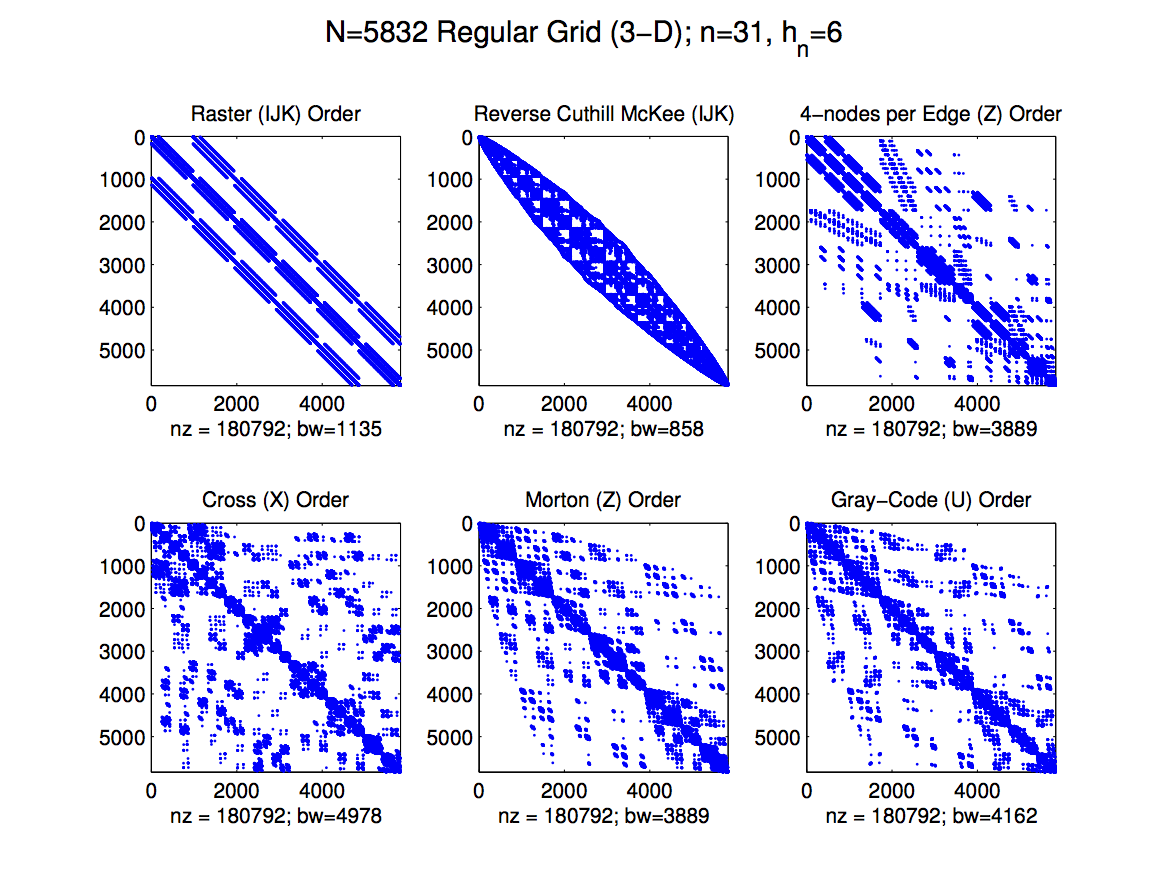
\includegraphics[width=0.95\textwidth]{rbffd_methods_content/hashing/spy_regulargrid_N18d3_n31_hn6.png} 
\caption{Impact of node orderings on an $N=18^3$ regular grid in 3-D. Stencil size $n=31$, fixed-grid resolution $(h_n)^d=6^3$. }
\label{fig:ordering_impact_rg}
\end{figure}

\begin{figure}
\centering
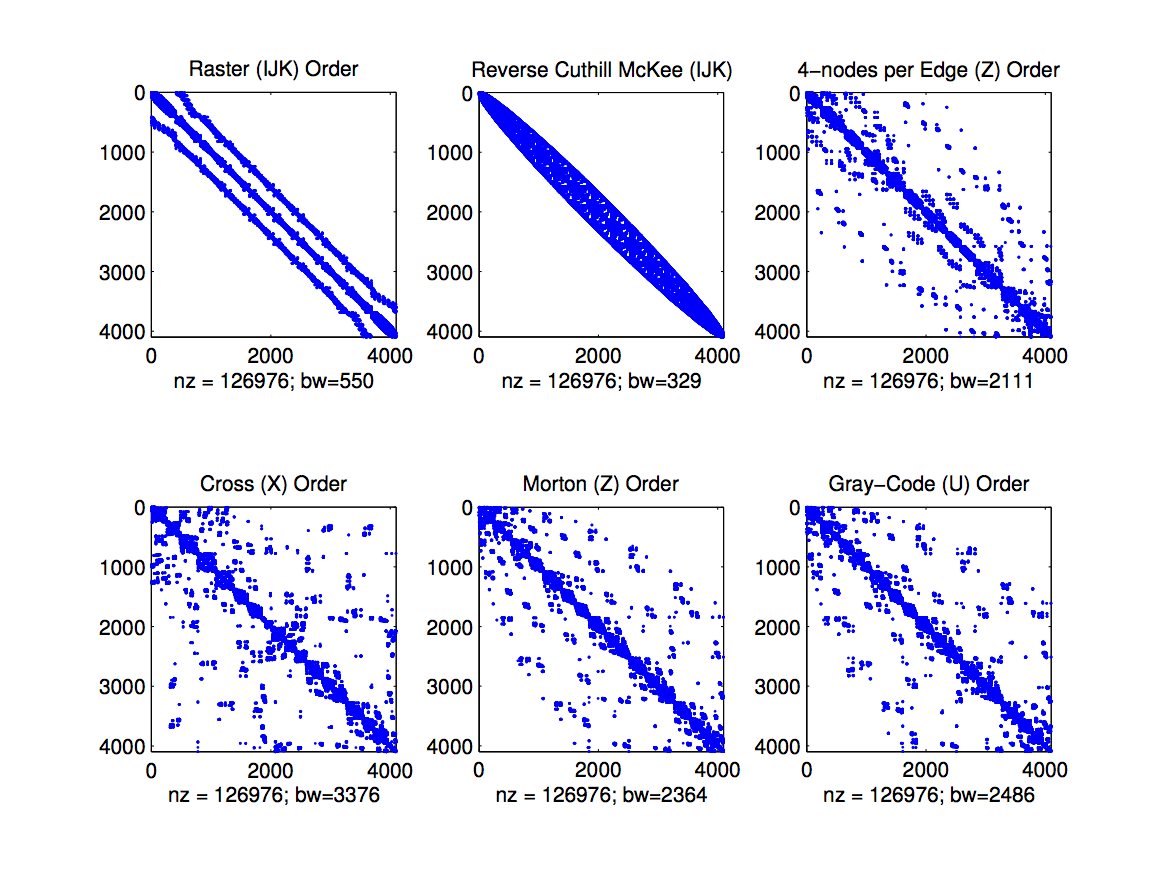
\includegraphics[width=0.95\textwidth]{rbffd_methods_content/hashing/dm_node_orderings_md4096_n31_hn10.png} 
\caption{ The impact of reordering on sparsity patterns for $N=4096$ MD nodes on the sphere. Stencil size $n=31$, fixed-grid resolution per dimension $h_n=10$. }
\label{fig:ordering_impact_cvt}
\end{figure}

\begin{table}[h]\footnotesize
  \centering
  \caption{Ordering Comparison for $N=10^6$ CVT unit sphere. Input nodes are quasi-random and test the best-case scenario for reordering improvements. Stencil size $n=50$, fixed-grid resolution $h_n=160$.}
  \label{tbl:ordering_impact}
  \begin{tabular}{ c | c | c | c | c | c | c }
               & IJK & RCM & Z & X & U & 4-node Z \\
               \hline
   Bandwidth   &  7885	& 6566	& 575606 &	819312 & 611513 & 513579   \\
   \hline
   SpMV Speedup & 1 &	1.09 & 1.06 & 1.06 & 1.04 & 0.94 \\
  \end{tabular}
\end{table}


%\begin{table}[h]\footnotesize
%  \centering
%  \caption{Ordering Comparison for $N=10^5$ CVT unit sphere. Stencil size $n=50$, fixed-grid resolution, $h_n=100$}
%  \begin{tabular}{ c | c | c | c | c | c | c }
%               & IJK & RCM & Z & X & U & 4-node Z \\
%               \hline
%   Bandwidth   &  8209	& 12973	 & 70545	& 87983 & 73699 & 70573   \\
%   \hline
%   SpMV Speedup vs IJK & 1 &	1.005 & 1.004 & 0.98 & 1.01 & 1.01 \\
%  \end{tabular}
%\end{table}

%TODO: possibility that majority of non-zeros are clustered near diagonal and outliers are deceiving the bandwidth metric. 


\section{Conclusion and Future Work}

This chapter introduced a fixed-grid method for RBF-FD stencil generation, and compared it to an efficient implementation of $k$-D Tree. The method proves itself capable of generating stencils twice as fast as $k$-D Tree.  
%---previously employed in work on RBF Partition of Unity schemes \cite{WendlandBook,Wendland2002} and 
%particle-based methods like Smoothed Particle Hydrodynamics \cite{Johnson2011,Green2010,Krog2010}---never 
%to RBF collocation method or RBF-FD---
Reordering nodes during stencil generation improves later performance of some RBF-FD solutions by a factor of five, but with the help of bit-interleaving and space filling curves that performance can be boosted slightly more.

In addition to ordering nodes based on space filling curves, a bandwidth reduction algorithm named Reverse Cuthill-McKee was also employed to reorder the differentiation matrix. Reverse Cuthill-McKee results show that not only is the algorithm exceptional at reducing the bandwidth, it also results in the most improvement to SpMV benchmarks. 

The implementation benchmarked above was developed as a pure CPU prototype with minimal attention to optimization. Although RBF-FD only requires neighbor queries once, the fixed-grid method's long lasting positive impact on memory is sufficient to justify its continued use. 

The C++ fixed-grid stencil generator defaults to the Raster-/IJK-order due to its ability to produce consistently small bandwidths. For situations when reordering is necessary for the best performance, the Reverse Cuthill-McKee algorithm is employed. In order to avoid MATLAB, RBF-FD applications in C++ rely on an implementation of the Cuthill-McKee algorithm provided by the BOOST library \cite{BoostSite}. 


%TODO: Similar conclusions are drawn by the authors of \cite{MellorCrummey2001}, who found that reordering nodes via RCM and space filling curves offer similar benefits in terms of reduced TLB misses and better cache coherency. 


Due to the limited significance of stencil generation under RBF-FD, the overhead in implementing and debugging a GPU implementation of the fixed-grid method is hard to justify. No known investigations consider RBF-FD on moving nodes (e.g., for adaptive node refinement like \cite{FlyerLehto10}), although such research should find the fixed-grid method significantly relevant. Future work in this direction would easily justify a GPU implementation following \cite{Krog2010,Green2010,Johnson2011, Goswami2010}. 

It also is worth noting that recent work by Connor and Kumar \cite{Connor2009} developed operators to directly transform floating point coordinates into $Z$-orderings. The MATLAB fixed-grid prototype (\cite{BolligRBFFixedGrid}) includes a test of those operators, although the investigation is incomplete. Preliminary results are shown in Figure~\ref{fig:float_z_results}. A set of nodes are distributed in $[0,20]^2$ with $d_x = 1.0$ ($d_y = d_x$) in Figure~\ref{fig:connor_works}. Node coordinates are floating point representations of integer values, and the curve drawn shows the successful reproduction of a Z-ordering over the nodes. In Figure~\ref{fig:connor_works2}, the same nodes are scaled to $d_x = 3.0$ (i.e., still integer representations). A number of 3-node Z's appear at coordinates that are multiples of powers of two, but that  is an anticipated flaw in the algorithm. The implementation fails when nodes are scaled to non-integer coordinates with $d_x = 0.3$ (Figure~\ref{fig:connor_fails}) and $d_x=0.05$ (Figure~\ref{fig:connor_fails2}). 

At this time, investigation into floating point Z-ordering is on hold as there is no urgent need for such an algorithm in RBF-FD. Direct communication with the lead author of \cite{Connor2009} attributed the errors in Figures~\ref{fig:connor_fails} and \ref{fig:connor_fails2} to unexpected behavior/handling of doubles in MATLAB, or an unforeseen error in the design of their algorithm. The author indicated the possibility that these cases were not considered during testing.

\begin{figure}
\begin{subfigure}[t]{0.5\textwidth}
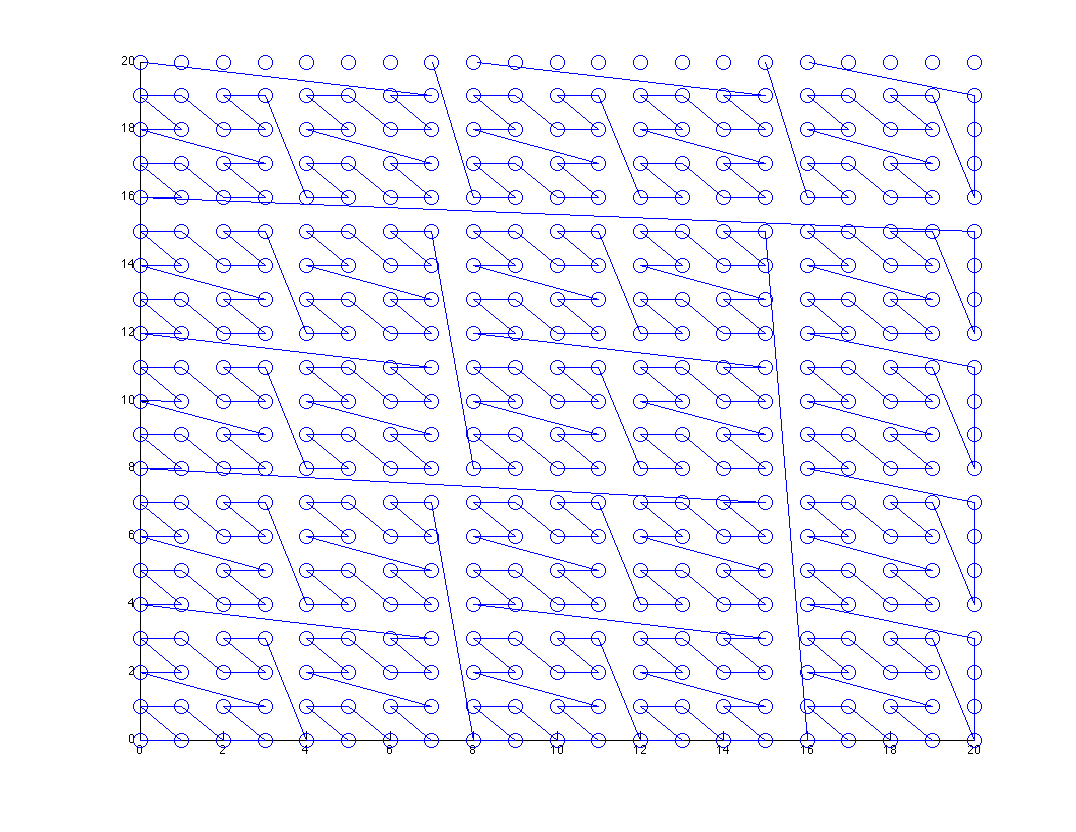
\includegraphics[width=\textwidth]{stencils_content/20x20.png}
\caption{Nodes in range $[0,20]^2$, $d_x = d_y = 1$.}
\label{fig:connor_works}
\end{subfigure}
\begin{subfigure}[t]{0.5\textwidth}
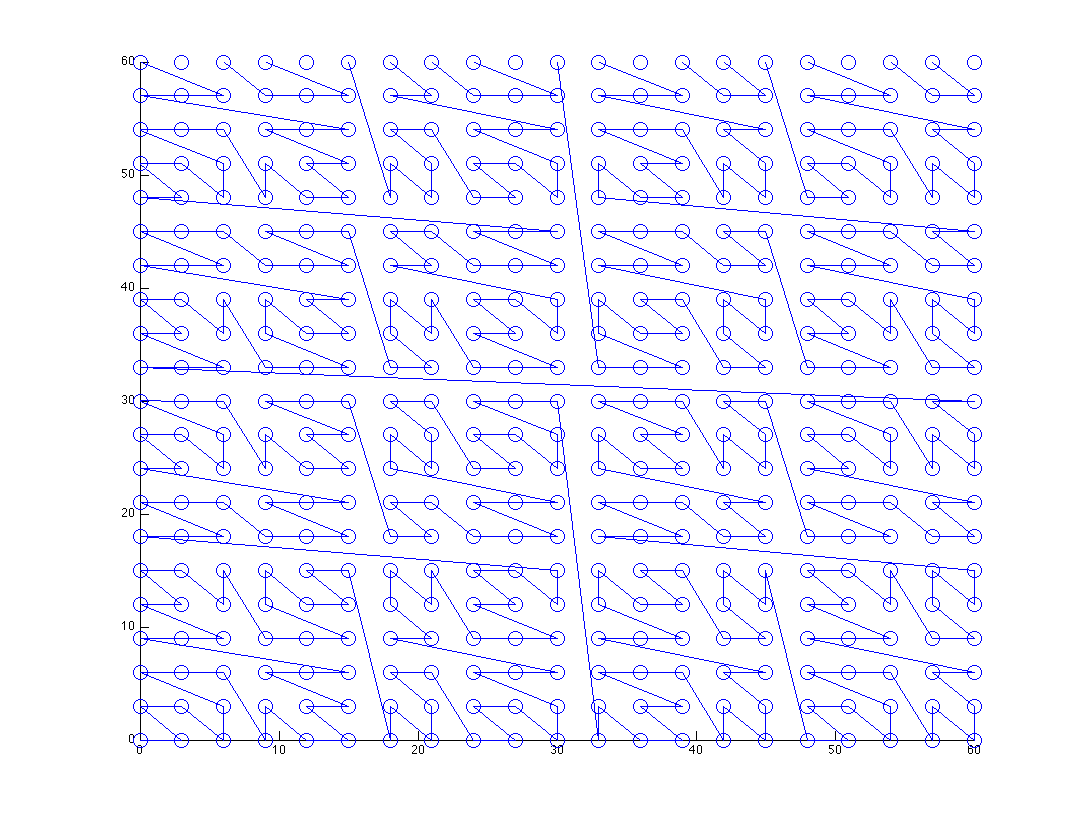
\includegraphics[width=\textwidth]{stencils_content/scale3.png}
\caption{Nodes in range $[0,60]^2$, $d_x = d_y = 3$.}
\label{fig:connor_works2}
\end{subfigure}
\begin{subfigure}[t]{0.5\textwidth}
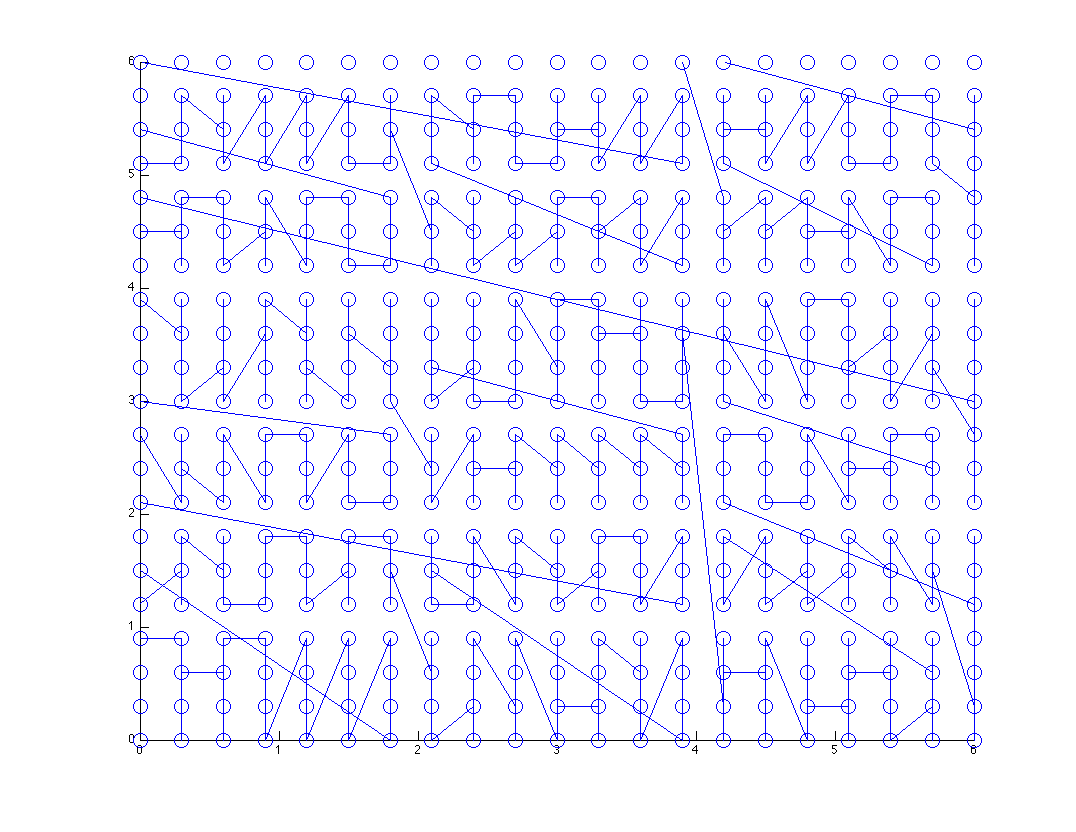
\includegraphics[width=\textwidth]{stencils_content/scale3em1.png}
\caption{Nodes in range $[0,6]^2$, $d_x = d_y = 0.3$.  }
\label{fig:connor_fails}
\end{subfigure}
\begin{subfigure}[t]{0.5\textwidth}
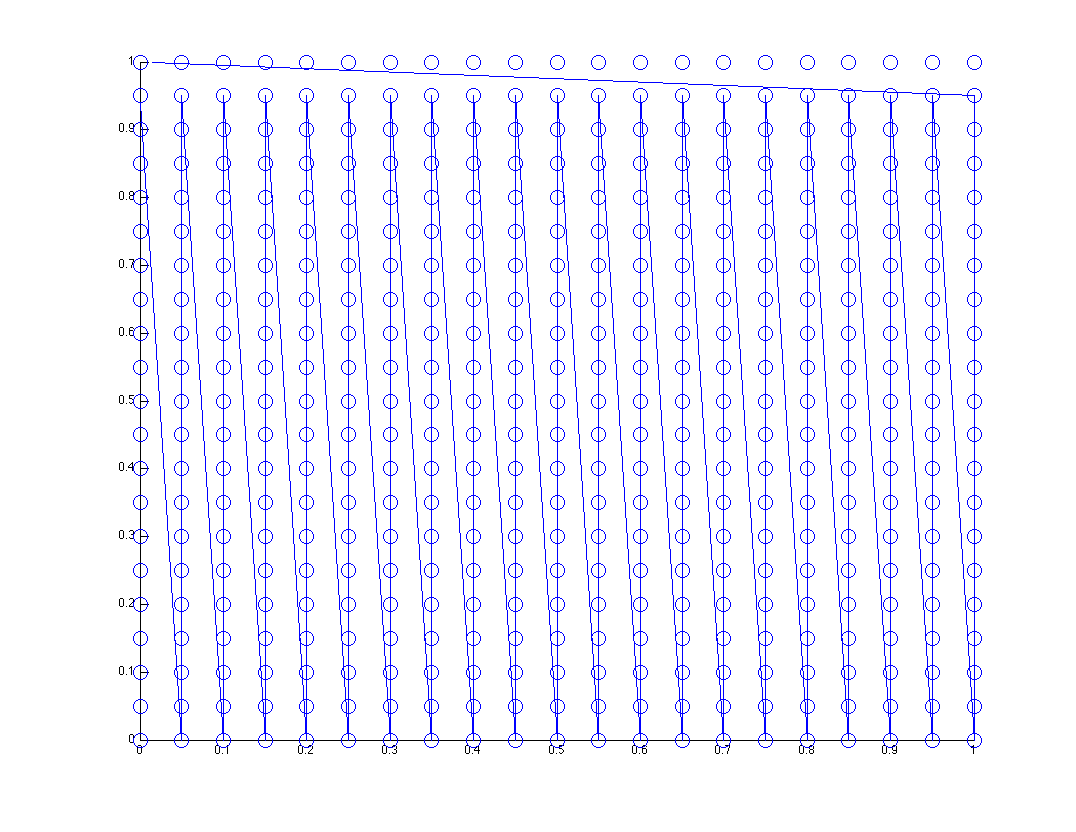
\includegraphics[width=\textwidth]{stencils_content/range0_1.png}
\caption{Nodes in range $[0,1]^2$, $d_x = d_y = 0.05$. }
\label{fig:connor_fails2}
\end{subfigure}
\caption{Preliminary results from $Z$-ordering nodes based on  (double precision) floating point node coordinates (following algorithm in \cite{Connor2009}). Our implementation functions well on integer coordinates when nodes are floating point representations of integers separated by $d_x = 1$ (a). Increasing $d_x$ extends some edges to 3-node Z's, but is mostly correct (b). The implementation fails when nodes are not representations of integers (c) and (d).}
\label{fig:float_z_results}
\end{figure}


\ifstandalone
\bibliographystyle{plain}
\bibliography{merged_references}
\end{document}
\else
\expandafter\endinput
\fi

\makeatletter
\@ifundefined{standalonetrue}{\newif\ifstandalone}{}
\@ifundefined{section}{\standalonetrue}{\standalonefalse}
\makeatother
\ifstandalone
\documentclass{report}

\usepackage{textcase}
%\usepackage{hyperref}
%\hypersetup{breaklinks=true}


% Added packages
\usepackage[usenames]{color}
\usepackage{amsfonts, amsmath, amssymb, graphics}

% NOTE: bibentry MUST appear before the hyperref or build will fail
\usepackage{bibentry}
\nobibliography*
\usepackage[square,sort,comma,numbers]{natbib}
  
\usepackage{float}
\usepackage[
	hidelinks,%
    %hyperindex=true,		% Make numbers of index links as well
   	backref=page, 		% Provide page listing where refs occur in the bibliography
	%breaklinks=true,
    %colorlinks,%
    %citecolor=green,%
    %filecolor=blue,%
    %linkcolor=red,%
    %urlcolor=red, 
]{hyperref}

\usepackage{dsfont}
%%%% USEPACKAGES for MACROS %%%%%
\usepackage{algpseudocode}
\usepackage[chapter]{algorithm}
%\usepackage{caption}
\usepackage{subcaption}
\usepackage{url}

\usepackage{array}
\usepackage{arydshln}
\usepackage{multirow}
\usepackage{multicol}
%\usepackage[section]{placeins}

\usepackage[usenames,dvipsnames]{color}
%\usepackage[english]{babel}
\usepackage{tabularx}
\usepackage{soul}
\usepackage{xparse}
\usepackage{listings}
%\usepackage[normalem]{ulem}



%%%%%%%%%%%%%%%
% Show a list of items "todo" or "done" 
% USAGE: 
% \begin{todolist} 
% 	\todo Something not finished
% 	\done Something finished
% \end{todolist} 
\newenvironment{todolist}{%
  \begin{list}{}{}% whatever you want the list to be
  \let\olditem\item
  \renewcommand\item{\olditem \textcolor{red}{(TODO)}: }
  \newcommand\todo{\olditem \textcolor{red}{(TODO)}: }
   \newcommand\done{\olditem \textcolor{ForestGreen}{(DONE)}: }
}{%
  \end{list}
} 
%%%%%%%%%%%%%%%

%%%%%%%%%%%%%%%
% Show a Author's Note
% USAGE: 
% \incomplete[Optional footnote message to further clarify note]{The text which is currently not finished}
\DeclareDocumentCommand \incomplete{ o m }
{%
\IfNoValueTF {#1}
{\textcolor{red}{Incomplete: \ul{#2}}} 
{\textcolor{red}{Incomplete: \ul{#2}}\footnote{Comment: #1}}%
}
%%%%%%%%%%%%%%%



%%%%%%%%%%%%%%%
% Show a Author's Note
% USAGE: 
% \authnote[Optional footnote message to further clarify note]{The note to your readers}
\DeclareDocumentCommand \authnote { o m }
{%
\IfNoValueTF {#1}
{\textcolor{blue}{Author's Note: \ul{#2}}} 
{\textcolor{blue}{Author's Note: \ul{#2}}\footnote{Comment: #1}}%
}
%%%%%%%%%%%%%%%



%%%%%%%%%%%%%%%
% Strike out text that doesn't belong in the paper
% USAGE: 
% \strike[Optional footnote to state why it doesn't belong]{Text to strike out}
\DeclareDocumentCommand \strike { o m }
{%
\setstcolor{Red}
\IfNoValueTF {#1}
{\textcolor{Gray}{\st{#2}}} 
{\textcolor{Gray}{\st{#2}}\footnote{Comment: #1}}%
}
%%%%%%%%%%%%%%%

\definecolor{light-gray}{gray}{0.95}

\newcommand{\cbox}[3]{
\ \\
\fcolorbox{#1}{#2}{
\parbox{\textwidth}{
#3
}
}
}

% Setup an environment similar to verbatim but which will highlight any bash commands we have
\lstnewenvironment{unixcmds}[0]
{
%\lstset{language=bash,frame=shadowbox,rulesepcolor=\color{blue}}
\lstset{ %
language=sh,		% Language
basicstyle=\ttfamily,
backgroundcolor=\color{light-gray}, 
rulecolor=\color{blue},
%frame=tb, 
columns=fullflexible,
%framexrightmargin=-.2\textwidth,
linewidth=0.8\textwidth,
breaklines=true,
%prebreak=/, 
  prebreak = \raisebox{0ex}[0ex][0ex]{\ensuremath{\hookleftarrow}},
%basicstyle=\footnotesize,       % the size of the fonts that are used for the code
%numbers=left,                   % where to put the line-numbers
%numberstyle=\footnotesize,      % the size of the fonts that are used for the line-numbers
%stepnumber=2,                   % the step between two line-numbers. If it's 1 each line 
                                % will be numbered
%numbersep=5pt,                  % how far the line-numbers are from the code
showspaces=false,               % show spaces adding particular underscores
showstringspaces=false,         % underline spaces within strings
showtabs=false,                 % show tabs within strings adding particular underscores
frame=single,	                % adds a frame around the code
tabsize=2,	                % sets default tabsize to 2 spaces
captionpos=b,                   % sets the caption-position to bottom
breakatwhitespace=false,        % sets if automatic breaks should only happen at whitespace
}
} { }

% Setup an environment similar to verbatim but which will highlight any bash commands we have
\lstnewenvironment{cppcode}[1]
{
%\lstset{language=bash,frame=shadowbox,rulesepcolor=\color{blue}}
\lstset{ %
	backgroundcolor=\color{light-gray}, 
	rulecolor=\color[rgb]{0.133,0.545,0.133},
	tabsize=4,
	language=[GNU]C++,
%	basicstyle=\ttfamily,
        basicstyle=\scriptsize,
        upquote=true,
        aboveskip={1.5\baselineskip},
        columns=fullflexible,
        %framexrightmargin=-.1\textwidth,
       %framexleftmargin=6mm,
        showstringspaces=false,
        extendedchars=true,
        breaklines=true,
        prebreak = \raisebox{0ex}[0ex][0ex]{\ensuremath{\hookleftarrow}},
        frame=single,
        showtabs=false,
        showspaces=false,
        showstringspaces=false,
        numbers=left,                   % where to put the line-numbers
	numberstyle=\footnotesize,      % the size of the fonts that are used for the line-numbers
	stepnumber=4,                   % the step between two line-numbers. If it's 1 each line 
                                % will be numbered
	firstnumber=#1,
         numbersep=5pt,                  % how far the line-numbers are from the code
        identifierstyle=\ttfamily,
        keywordstyle=\color[rgb]{0,0,1},
        commentstyle=\color[rgb]{0.133,0.545,0.133},
        stringstyle=\color[rgb]{0.627,0.126,0.941},
}
} { }

% Setup an environment similar to verbatim but which will highlight any bash commands we have
\lstnewenvironment{mcode}[1]
{
\lstset{ %
	backgroundcolor=\color{light-gray}, 
	rulecolor=\color[rgb]{0.133,0.545,0.133},
	tabsize=4,
	language=Matlab,
%	basicstyle=\ttfamily,
        basicstyle=\scriptsize,
        upquote=true,
        aboveskip={1.5\baselineskip},
        columns=fullflexible,
        %framexrightmargin=-.1\textwidth,
       %framexleftmargin=6mm,
        showstringspaces=false,
        extendedchars=true,
        breaklines=true,
        prebreak = \raisebox{0ex}[0ex][0ex]{\ensuremath{\hookleftarrow}},
        frame=single,
        showtabs=false,
        showspaces=false,
        showstringspaces=false,
        numbers=left,                   % where to put the line-numbers
	numberstyle=\footnotesize,      % the size of the fonts that are used for the line-numbers
	stepnumber=4,                   % the step between two line-numbers. If it's 1 each line 
                                % will be numbered
	firstnumber=#1,
         numbersep=5pt,                  % how far the line-numbers are from the code
        identifierstyle=\ttfamily,
        keywordstyle=\color[rgb]{0,0,1},
        commentstyle=\color[rgb]{0.133,0.545,0.133},
        stringstyle=\color[rgb]{0.627,0.126,0.941},
}
} { }

\newcommand{\inputmcode}[1]{%
\lstset{ %
	backgroundcolor=\color{light-gray},  %
	rulecolor=\color[rgb]{0.133,0.545,0.133}, %
	tabsize=4, %
	language=Matlab, %
%	basicstyle=\ttfamily,
        basicstyle=\scriptsize, %
        %        upquote=true,
        aboveskip={1.5\baselineskip}, %
        columns=fullflexible, %
        %framexrightmargin=-.1\textwidth,
       %framexleftmargin=6mm,
        showstringspaces=false, %
        extendedchars=true, %
        breaklines=true, %
        prebreak = \raisebox{0ex}[0ex][0ex]{\ensuremath{\hookleftarrow}}, %
        frame=single, %
        showtabs=false, %
        showspaces=false, %
        showstringspaces=false,%
        numbers=left,                   % where to put the line-numbers
	numberstyle=\footnotesize,      % the size of the fonts that are used for the line-numbers
	stepnumber=4,                   % the step between two line-numbers. If it's 1 each line 
                                % will be numbered
         numbersep=5pt,                  % how far the line-numbers are from the code
        identifierstyle=\ttfamily, %
        keywordstyle=\color[rgb]{0,0,1}, %
        commentstyle=\color[rgb]{0.133,0.545,0.133}, %
        stringstyle=\color[rgb]{0.627,0.126,0.941} %
}
\lstinputlisting{#1}%
}

%\lstset{ %
%	backgroundcolor=\color{light-gray}, 
%	rulecolor=\color[rgb]{0.133,0.545,0.133},
%	tabsize=4,
%	language=Matlab,
%%	basicstyle=\ttfamily,
%        basicstyle=\scriptsize,
%        upquote=true,
%        aboveskip={1.5\baselineskip},
%        columns=fullflexible,
%        %framexrightmargin=-.1\textwidth,
%       %framexleftmargin=6mm,
%        showstringspaces=false,
%        extendedchars=true,
%        breaklines=true,
%        prebreak = \raisebox{0ex}[0ex][0ex]{\ensuremath{\hookleftarrow}},
%        frame=single,
%        showtabs=false,
%        showspaces=false,
%        showstringspaces=false,
%        numbers=left,                   % where to put the line-numbers
%	numberstyle=\footnotesize,      % the size of the fonts that are used for the line-numbers
%	stepnumber=4,                   % the step between two line-numbers. If it's 1 each line 
%                                % will be numbered
%	firstnumber=#1,
%         numbersep=5pt,                  % how far the line-numbers are from the code
%        identifierstyle=\ttfamily,
%        keywordstyle=\color[rgb]{0,0,1},
%        commentstyle=\color[rgb]{0.133,0.545,0.133},
%        stringstyle=\color[rgb]{0.627,0.126,0.941},
%}


\newcommand{\Laplacian}[1]{\nabla^2 #1}

% set of all nodes received and contained on GPU
\newcommand{\setAllNodes}[0]{\mathcal{G}}
% set of stencil centers on GPU
\newcommand{\setCenters}[0]{\mathcal{Q}}
% set of stencil centers with nodes in \setDepend
\newcommand{\setBoundary}[0]{\mathcal{B}}
% set of nodes received by other GPUs
\newcommand{\setDepend}[0]{\mathcal{R}}
% set of nodes sent to other GPUs
\newcommand{\setProvide}[0]{\mathcal{O}}


\newcommand{\toprule}[0]{\hline}
\newcommand{\midrule}[0]{\hline\hline}
\newcommand{\bottomrule}[0]{\hline}

\newcolumntype{C}{>{\centering\arraybackslash}b{1in}}
\newcolumntype{L}{>{\flushleft\arraybackslash}b{1.5in}}
\newcolumntype{R}{>{\flushright\arraybackslash}b{1.5in}}
\newcolumntype{D}{>{\flushright\arraybackslash}b{2.0in}}
\newcolumntype{E}{>{\flushright\arraybackslash}b{1.0in}}

\DeclareSymbolFont{AMSb}{U}{msb}{m}{n}
\DeclareMathSymbol{\N}{\mathbin}{AMSb}{"4E}
\DeclareMathSymbol{\Z}{\mathbin}{AMSb}{"5A}
\DeclareMathSymbol{\R}{\mathbin}{AMSb}{"52}
\DeclareMathSymbol{\Q}{\mathbin}{AMSb}{"51}
\DeclareMathSymbol{\PP}{\mathbin}{AMSb}{"50}
\DeclareMathSymbol{\I}{\mathbin}{AMSb}{"49}
%\DeclareMathSymbol{\C}{\mathbin}{AMSb}{"43}

%%%%%% VECTOR NORM: %%%%%%%
\newcommand{\vectornorm}[1]{\left|\left|#1\right|\right|}
\newcommand{\vnorm}[1]{\left|\left|#1\right|\right|}
\newcommand{\by}[0]{\times}
\newcommand{\vect}[1]{\mathbf{#1}}
%\newcommand{\mat}[1]{\mathbf{#1}} 

%\renewcommand{\vec}[1]{ \textbf{#1} }
%%%%%%%%%%%%%%%%%%%%%%

%%%%%%% THM, COR, DEF %%%%%%%
%\newtheorem{theorem}{Theorem}[section]
%\newtheorem{lemma}[theorem]{Lemma}
%\newtheorem{proposition}[theorem]{Proposition}
%\newtheorem{corollary}[theorem]{Corollary}
%\newenvironment{proof}[1][Proof]{\begin{trivlist}
%\item[\hskip \labelsep {\bfseries #1}]}{\end{trivlist}}
%\newenvironment{definition}[1][Definition]{\begin{trivlist}
%\item[\hskip \labelsep {\bfseries #1}]}{\end{trivlist}}
%\newenvironment{example}[1][Example]{\begin{trivlist}
%\item[\hskip \labelsep {\bfseries #1}]}{\end{trivlist}}
%\newenvironment{remark}[1][Remark]{\begin{trivlist}
%\item[\hskip \labelsep {\bfseries #1}]}{\end{trivlist}}
%\newcommand{\qed}{\nobreak \ifvmode \relax \else
%      \ifdim\lastskip<1.5em \hskip-\lastskip
%      \hskip1.5em plus0em minus0.5em \fi \nobreak
%      \vrule height0.75em width0.5em depth0.25em\fi}
%%%%%%%%%%%%%%%%%%%%%%

%
%\usepackage[algochapter]{algorithm2e}
%\usepackage[usenames]{color}
% colors to show the corrections
\newcommand{\red}[1]{\textbf{\textcolor{red}{#1}}}
\newcommand{\blue}[1]{\textbf{\textcolor{blue}{#1}}}
\newcommand{\cyan}[1]{\textbf{\textcolor{cyan}{#1}}}
\newcommand{\green}[1]{\textbf{\textcolor{green}{#1}}}
\newcommand{\magenta}[1]{\textbf{\textcolor{magenta}{#1}}}
\newcommand{\orange}[1]{\textbf{\textcolor{orange}{#1}}}
%%%%%%%%%% DK DK
% comments between authors
\newcommand{\toall}[1]{\textbf{\green{@@@ All: #1 @@@}}}
\newcommand{\toevan}[1]{\textbf{\red{*** Evan: #1 ***}}}
%\newcommand{\toevan}[1]{}  % USE FOR FINAL VERSION
\newcommand{\toe}[1]{\textbf{\red{*** Evan: #1 ***}}}
\newcommand{\tog}[1]{\textbf{\blue{*** Gordon: #1 ***}}}
%\newcommand{\togordon}[1]{\textbf{\blue{*** Gordon: #1 ***}}}
\renewcommand{\ge}[3]{{\textcolor{blue}{*** \textbf{Gordon:}\strike{#1} #2 ***}}\red{(#3)}}
\renewcommand{\ge}[3]{{\textcolor{blue}{#2}}}
\renewcommand{\ge}[3]{{\textcolor{Red}{#2}}}
\newcommand{\eb}[3]{{\textcolor{Red}{*** \textbf{Evan:}\strike{#1} #2 ***}}\red{(#3)}}
\renewcommand{\eb}[3]{{{\textcolor{Red}{#2}}}}
%\def\ge#1#2#3{}{\textbf{\blue{*** Gordon: #2 ***}}}{(#3)}
\newcommand{\gee}[1]{{\bf{\blue{{\em #1}}}}}
\newcommand{\old}[1]{}
\newcommand{\del}[1]{***#1*** }



% \DeclareMathOperator{\Sample}{Sample}
%\let\vaccent=\v % rename builtin command \v{} to \vaccent{}
%\renewcommand{\vec}[1]{\ensuremath{\mathbf{#1}}} % for vectors
\newcommand{\gv}[1]{\ensuremath{\mbox{\boldmath$ #1 $}}} 
% for vectors of Greek letters
\newcommand{\uv}[1]{\ensuremath{\mathbf{\hat{#1}}}} % for unit vector
\newcommand{\abs}[1]{\left| #1 \right|} % for absolute value
\newcommand{\avg}[1]{\left< #1 \right>} % for average
\let\underdot=\d % rename builtin command \d{} to \underdot{}
\renewcommand{\d}[2]{\frac{d #1}{d #2}} % for derivatives
\newcommand{\dd}[2]{\frac{d^2 #1}{d #2^2}} % for double derivatives
\newcommand{\pd}[2]{\frac{\partial #1}{\partial #2}} 
% for partial derivatives
\newcommand{\pdd}[2]{\frac{\partial^2 #1}{\partial #2^2}} 
\newcommand{\pdda}[3]{\frac{\partial^2 #1}{\partial #2 \partial #3}} 
% for double partial derivatives
\newcommand{\pdc}[3]{\left( \frac{\partial #1}{\partial #2}
 \right)_{#3}} % for thermodynamic partial derivatives
\newcommand{\ket}[1]{\left| #1 \right>} % for Dirac bras
\newcommand{\bra}[1]{\left< #1 \right|} % for Dirac kets
\newcommand{\braket}[2]{\left< #1 \vphantom{#2} \right|
 \left. #2 \vphantom{#1} \right>} % for Dirac brackets
\newcommand{\matrixel}[3]{\left< #1 \vphantom{#2#3} \right|
 #2 \left| #3 \vphantom{#1#2} \right>} % for Dirac matrix elements
\newcommand{\grad}[1]{\gv{\nabla} #1} % for gradient
\let\divsymb=\div % rename builtin command \div to \divsymb
\renewcommand{\div}[1]{\gv{\nabla} \cdot #1} % for divergence
\newcommand{\curl}[1]{\gv{\nabla} \times #1} % for curl
\let\baraccent=\= % rename builtin command \= to \baraccent
\renewcommand{\=}[1]{\stackrel{#1}{=}} % for putting numbers above =
\newcommand{\diffop}[1]{\mathcal{L}#1}
\newcommand{\boundop}[1]{\mathcal{B}#1}
\newcommand{\rvec}[0]{{\bf r}}

\newcommand{\Interior}[0]{\Omega}
\newcommand{\domain}[0]{\Omega}
%\newcommand{\Boundary}[0]{\partial \Omega}
\newcommand{\Boundary}[0]{\Gamma}

\newcommand{\on}[1]{\hskip1.5em \textrm{ on } #1}

\newcommand{\gemm}{\texttt{GEMM}}
\newcommand{\trmm}{\texttt{TRMM}}
\newcommand{\gesvd}{\texttt{GESVD}}
\newcommand{\geqrf}{\texttt{GEQRF}}


\newcommand{\minitab}[2][l]{\begin{tabular}{#1}#2\end{tabular}}
\newcommand{\comm}[1]{\textcolor{red}{\textit{#1}}}

\newcommand{\nfrac}[2]{
\nicefrac{#1}{#2}
%\frac{#1}{#2}
}

\usepackage{xparse}
\usepackage{soul}


%%%%%%%%%%%%%%%
% Show a Author's Note
% USAGE: 
% \incomplete[Optional footnote message to further clarify note]{The text which is currently not finished}
\DeclareDocumentCommand \incomplete{ o m }
{%
\IfNoValueTF {#1}
{\textcolor{red}{Incomplete: \ul{#2}}} 
{\textcolor{red}{Incomplete: \ul{#2}}\footnote{Comment: #1}}%
}
%%%%%%%%%%%%%%%



%%%%%%%%%%%%%%%
% Show a Author's Note
% USAGE: 
% \authnote[Optional footnote message to further clarify note]{The note to your readers}
\DeclareDocumentCommand \authnote { o m }
{%
\IfNoValueTF {#1}
{\textcolor{blue}{Author's Note: \ul{#2}}} 
{\textcolor{blue}{Author's Note: \ul{#2}}\footnote{Comment: #1}}%
}
%%%%%%%%%%%%%%%



%%%%%%%%%%%%%%%
% Strike out text that doesn't belong in the paper
% USAGE: 
% \strike[Optional footnote to state why it doesn't belong]{Text to strike out}
\DeclareDocumentCommand \strike { o m }
{%
\setstcolor{red}
\IfNoValueTF {#1}
{\textcolor{Gray}{\st{#2}}} 
{\textcolor{Gray}{\st{#2}}\footnote{Comment: #1}}%
}
%%%%%%%%%%%%%%%



%
% colors to show the corrections
\newcommand{\red}[1]{\textbf{\textcolor{red}{#1}}}
\newcommand{\blue}[1]{\textbf{\textcolor{blue}{#1}}}
\newcommand{\cyan}[1]{\textbf{\textcolor{cyan}{#1}}}
\newcommand{\green}[1]{\textbf{\textcolor{green}{#1}}}
\newcommand{\magenta}[1]{\textbf{\textcolor{magenta}{#1}}}
\newcommand{\orange}[1]{\textbf{\textcolor{orange}{#1}}}
%%%%%%%%%% DK DK
% comments between authors
\newcommand{\toall}[1]{\textbf{\green{@@@ All: #1 @@@}}}
\newcommand{\toevan}[1]{\textbf{\red{*** Evan: #1 ***}}}
%\newcommand{\toevan}[1]{}  % USE FOR FINAL VERSION
\newcommand{\toe}[1]{\textbf{\red{*** Evan: #1 ***}}}
\newcommand{\tog}[1]{\textbf{\blue{*** Gordon: #1 ***}}}
%\newcommand{\togordon}[1]{\textbf{\blue{*** Gordon: #1 ***}}}
\renewcommand{\ge}[3]{{\textcolor{blue}{*** \textbf{Gordon:}\strike{#1} #2 ***}}\red{(#3)}}
\renewcommand{\ge}[3]{{\textcolor{blue}{#2}}}
\renewcommand{\ge}[3]{{\textcolor{red}{#2}}}
\newcommand{\eb}[3]{{\textcolor{red}{*** \textbf{Evan:}\strike{#1} #2 ***}}\red{(#3)}}
\renewcommand{\eb}[3]{{{\textcolor{red}{#2}}}}
%\def\ge#1#2#3{}{\textbf{\blue{*** Gordon: #2 ***}}}{(#3)}
\newcommand{\gee}[1]{{\bf{\blue{{\em #1}}}}}
\newcommand{\old}[1]{}
\newcommand{\del}[1]{***#1*** }



% Rename  this file          misc_mac.tex
%----------------------------------------------------------------------
%%%%%%%%%%%%%%%%%%%%%%%%%%%%%%%%%%%%%%%%%%%%%%%%%%%%%%%%%%%%%%%%%%%%%%%%%%%%%%%
%
%	Math Symbols   Math Symbols   Math Symbols   Math Symbols   
%
%%%%%%%%%%%%%%%%%%%%%%%%%%%%%%%%%%%%%%%%%%%%%%%%%%%%%%%%%%%%%%%%%%%%%%%%%%%%%%%
\def\pmb#1{\setbox0=\hbox{$#1$}%
	\kern-.025em\copy0\kern-\wd0
	\kern.05em\copy0\kern-\wd0
	\kern-.025em\raise.0433em\box0}
\def\pmbf#1{\pmb#1}
\def\bfg#1{\pmb#1}

% BETTER VALUES FOR AUTOMATIC FIGURE PLACEMENT THAN THOSE PROVIDED BY 
% LATEX DEFAULTS.

\renewcommand{\textfloatsep}{1ex}
\renewcommand{\floatpagefraction}{0.9}
\renewcommand{\intextsep}{1ex}
\renewcommand{\topfraction}{.9}
\renewcommand{\bottomfraction}{.9}
\renewcommand{\textfraction}{.1}

% #1  position of floating figure (h|t|b|p)
% #1  EPS postscript file
% #2  size
% #3  caption

%usage of newfig:
%  \newfig{file.ps}{3in}{Fig1: this is a figure}

\input{epsf}
\def\newfig#1#2#3{
  \begin{figure}[htbp]
  \vspace{1ex}
  \setlength{\epsfxsize}{#2}
  \centerline{\epsfbox{#1}}
  \vspace{-.1in}\caption{\small #3}\break\vspace{.2in}
  \label{#1}
  \end{figure}
}

%usage of newfigtwo: 2 figures, vertically stacked
% \newfig
%	{file1.ps}
%	{file2.ps}
%	{width}
%	{vertical space}
%	{Caption}

\def\newfigtwo#1#2#3#4#5{
  \begin{figure}[htbp]
  \vspace{1ex}
  \setlength{\epsfxsize}{#3}
  \centerline{\epsfbox{#1}}
  \vspace{#4}
  \setlength{\epsfxsize}{#3}
  \centerline{\epsfbox{#2}}
  \vspace{-.1in}\caption{\small #5}\break\vspace{.2in}
  \label{#1}
  \end{figure}
}

\def\newfigh#1#2#3#4{  % add height specification
  \begin{figure}[htbp]
  \vspace{1ex}
  \setlength{\epsfxsize}{#2}
  \setlength{\epsfysize}{#4}
  \centerline{\epsfbox{#1}}
  \vspace{-.1in}\caption{\small #3}\break\vspace{.2in}
  \label{#1}
  \end{figure}
}

\def\herefig#1#2#3{
  \begin{figure}[h]
  \setlength{\epsfxsize}{#2}
  \centerline{\epsfbox{#1}}
  \caption{\small #3}
  \label{#1}
  \end{figure}
}

\def\etal{{{\em et~al.\,\,}}}
\def\note#1{\\ =====#1===== \\}
\def\FBOX#1{\ \\ \fbox{\begin{minipage}{5in}#1\end{minipage}}\\ }
\newcount\sectionno     \sectionno=0
\newcount\eqnum         \eqnum=0
\def\addeqno{\global\advance \eqnum by  1 }
\def\subeqno{\global\advance \eqnum by -1 }
%\def\eqn{\addeqno \eqno \hbox{(\number\sectionno.\number\eqnum)} }

\def\tildetilde#1{\tilde{\tilde{#1}}}
\def\barbar#1{\overbar{\overbar{#1}}}

\def\vsp#1{\vspace{#1 ex}}
\def\fpar{\hspace{\parindent}}
%
%  \pf : 2 arguments: numerator and denominator of partial derivative
%
\def\pf#1#2{{\frac{\partial{#1}}{\partial{#2}}}}
\def\pfs#1#2{{\partial_{#2}{#1}}}
\def\pftwo#1#2{{\frac{\partial^2{#1}}{\partial{#2}^2}}}
\def\pfxx#1#2{{\frac{\partial^2{#1}}{\partial{#2}^2}}}
%\def\pfxy#1#2{{\frac{\partial^2{#1}}{\partial{#2}\partial{#3}}}}
\def\pfn#1#2#3{{\frac{\partial^{#1}{#2}}{\partial{#3}^{#1}}}}
\def\df#1#2{{\frac{d{#1}}{d{#2}}}}
\def\dfn#1#2#3{{\frac{d^{#1}{#2}}{d{#3}^{#1}}}}
\def\Dt#1#2{\frac{D#1}{D#2}}
\def\dt#1#2{\frac{d#1}{d#2}}
\def\bld#1{{\bf #1}}
\def\pfp#1#2#3{\pf{}{#3}{\left(\frac{#1}{#2}\right)}}

\def\norm#1{\|#1\|}

%
% Graphic characters  (\dot already defined by TeX/LateX)
%
\def\dash{\rule[1.5pt]{2mm}{.3mm}\HS{.9mm}}
\def\dott{\rule[1.5pt]{.7mm}{.3mm}\HS{.7mm}}
\def\dashline{\dash\dash\dash}
\def\dotline{\dott\dott\dott\dott\dott\dott}
\def\dashdotline{\dash$\cdot$\HS{.9mm}\dash}
\def\solidline{\rule[2pt]{7mm}{.3mm}}
% 
% overcircle
%
\def\ovcircle#1{\buildrel{\circ}\over{#1}}
%\def\below#1#2{\buildrel{#2}\under{#1}}
%\def\above#1#2{\buildrel{#2}\over{#1}}
%
%  big parenthesis and brackets
%
\def\bigpar#1#2{{\left(\frac{#1}{#2}\right)}}
\def\bigbra#1#2{{\left\[\frac{#1}{#2}\right\]}}

\def\Lp{\left(}
\def\Rp{\right)}
\def\Lb{\left[}
\def\Rb{\right]}
\def\Ln{\left\langle}
\def\Rn{\right\rangle}
\def\Ld{\left.}
\def\Rd{\right.}
\def\Lv{\left|}
\def\Rv{\right|}
\def\Lbr{\left|}
\def\Rbr{\right|}
\def\lng{\langle}
\def\rng{\rangle}
\def\Lc{\left\{}
\def\Rc{\right\}}
%%% %

% Cannot be handled by Lyx
%\def\[{{[}}
%\def\]{{]}}

%
\def\eol{\nonumber \\}
\def\eolnonb{\nonumber\\}
\def\eolnb{\\}
\def\nonb{\nonumber}
\def\be{\begin{equation}}
\def\ee{\end{equation}}
\def\BEQNA{\begin{eqnarray}}
\def\EEQNA{\end{eqnarray}}
\def\eqa{&=&}
\def\beqna{\begin{eqnarray}}
\def\eeqna{\end{eqnarray}}
\def\bverb{\begin{verbatim}}
\def\everb{\end{verbatim}}
\def\VERB#1{\bverb #1 \everb}
\def\btbl{\begin{tabular}}
\def\etbl{\end{tabular}}
\def\bmini{\begin{minipage}[t]{5.5in}}
\def\emini{\end{minipage}}
\def\parray#1#2{\left(\begin{array}{#1}#2\end{array}\right)}
\def\barray#1#2{\left[\begin{array}{#1}#2\end{array}\right]}
\def\carray#1#2{\left\{\begin{array}{#1}#2\end{array}\right.}
\def\darray#1#2{\left|\begin{array}{#1}#2\end{array}\right|}

\def\BEGTABLE#1{\begin{table}[hbt]\vspace{2ex}\begin{center}\bmini\centering\btbl{#1}}
\def\ENDTABLE#1#2{\etbl\caption[#1]{#2}\EMINI\end{center}\vspace{2ex}\end{table}}

\def\bfltbl#1{\begin{table}[hbt]\vspace{2ex}\begin{center}\bmini\centering\btbl{#1}}
\def\efltbl#1#2{\etbl\caption[#1]{#2}\emini\end{center}\vspace{2ex}\end{table}}
\def\mcol{\multicolumn}
%
%  label equations with (#)
%
\def\reff#1{(\ref{#1})}
%
%  macros borrowed from viewgraph package
%

\newenvironment{LETTRS}[3]{\begin{letter}{#1}
\input{origin}\opening{Dear #2:}\input{#3}\closing{Sincerely yours,}\end{letter}}{\clearpage}

\newenvironment{VIEW}[1]{{\BC\Huge\bf #1 \EC}\LARGE\VS{.05in}}{\clearpage}

\def\RM#1{\rm{#1\ }}
\def\BV{\begin{VIEW}}
\def\EV{\end{VIEW}}

\def\NI{\noindent}

\def\VS{\vspace*}
\def\HS{\hspace*}
\def\IT{\item}

\def\BARR{\begin{array}}
\def\EARR{\end{array}}

\def\BPARR{\left(\begin{array}}
\def\EPARR{\end{array}\right)}

\def\BDET{\left|\begin{array}}
\def\EDET{\end{array}\right|}

\def\BDF{\begin{definition}}
\def\EDF{\end{definition}}

\def\BSU{\begin{block}{Summary}}
\def\ESU{\end{block}}

\def\BEX{\begin{example}}
\def\EEX{\end{example}}

\def\BTH{\begin{theorem}}
\def\ETH{\end{theorem}}

\def\BCO{\begin{corollary}}
\def\ECO{\end{corollary}}

\def\BPROOF{\begin{proof}}
\def\EPROOF{\end{proof}}

\def\BLM{\begin{lemma}}
\def\ELM{\end{lemma}}

\def\BEQ{\begin{equation}}
\def\EEQ{\end{equation}}

\def\BEQNNB{$$}
\def\EEQNNB{$$}

\def\BE{\begin{enumerate}}
\def\EE{\end{enumerate}}

\def\BD{\begin{description}}
\def\ED{\end{description}}

\def\BI{\begin{itemize}}
\def\EI{\end{itemize}}

\def\BC{\begin{center}}
\def\EC{\end{center}}

\def\BFIG{\begin{figure}}
\def\EFIG{\end{figure}}

\def\BTABB{\begin{tabbing}}
\def\ETABB{\end{tabbing}}

\def\BMINI{\begin{minipage}}
\def\EMINI{\end{minipage}}

\def\BTABLE{\begin{table}}
\def\ETABLE{\end{table}}

\def\BTABUL{\begin{tabular}}
\def\ETABUL{\end{tabular}}

\def\MCOL{\multicolumn}
\def\UL{\underline}
\def\ULL#1{\UL{\UL{#1}}}

\def\BDOC{\begin{document}}
\def\EDOC{\end{document}}

\def\EM#1{{\em #1\/}}
\def\FN{\footnote}

% Courtesy of Ugo Piomelli

\def\latexfig #1 #2 #3 #4 #5 {\ \vfill
\hfill\hbox to 0.05in{\vbox to #3truein{
         \special{psfile="#1" angle=270 hscale=100 
                  hoffset=#4 voffset=#5 vscale=100} }\hfill}
\hfill\vspace{-0.1in}        }

% #1 is the .ps filename
% #2 is not used in the present version
% #3 is the size of the white space left above the caption (in inches)
% #4 is the horizontal offset from some unknown reference point.
%    It is in 1/72 of an inch and is positive to the right.
% #5 is the vertical offset from some unknown reference point.
%    It is in 1/72 of an inch and is positive upwards.


\newcommand{\mathsym}[1]{{}}
\newcommand{\unicode}[1]{{}}
\newcommand{\ep}{\epsilon}
\newcommand{\vv}{\mathbf{v}}
\newcommand{\vu}{\mathbf{u}}
\newcommand{\vx}{\mathbf{x}}

\newcommand{\Laplacian}[1]{\nabla^2 #1}
\newcommand{\LaplaceBeltrami}[1]{\Delta_S #1}

% set of all nodes received and contained on GPU
\newcommand{\setAllNodes}[0]{\mathcal{G}}
% set of stencil centers on GPU
\newcommand{\setCenters}[0]{\mathcal{Q}}
% set of stencil centers with nodes in \setDepend
\newcommand{\setBoundary}[0]{\mathcal{B}}
% set of nodes received by other GPUs
\newcommand{\setDepend}[0]{\mathcal{R}}
% set of nodes sent to other GPUs
\newcommand{\setProvide}[0]{\mathcal{O}}





\usepackage{tabularx} 
\newcolumntype{C}{>{\centering\arraybackslash}b{1in}}
\newcolumntype{L}{>{\flushleft\arraybackslash}b{1.5in}}
\newcolumntype{R}{>{\flushright\arraybackslash}b{1.5in}}
\newcolumntype{D}{>{\flushright\arraybackslash}b{2.0in}}
\newcolumntype{E}{>{\flushright\arraybackslash}b{1.0in}}


 


%\usepackage{xcolor}

%\usepackage{refcheck}
% Sepia
%\definecolor{myBGcolor}{HTML}{F6F0D6}
%\definecolor{myTextcolor}{HTML}{4F452C}
% Dark
%\definecolor{myBGcolor}{HTML}{3E3535}
%\definecolor{myTextcolor}{HTML}{CFECEC}
%\color{myTextcolor}
%\pagecolor{myBGcolor}
 
\usepackage[margin=1.25in]{geometry}

\begin{document}
\fi

\chapter{GPU SpMV}
\label{chap:gpu_rbffd}

General Purpose GPU (GPGPU) computing is one of today's hottest trends in scientific computing. As problem sizes grow larger, it behooves us to work on parallel architectures, be it across multiple CPUs or one or more GPUs. With over 1 TFLOP/s peak possible throughput in double precision on a single GPU \cite{KeplerFactSheet}, a compelling argument is made for the latter. 

In the last decade, CPU designers have been forced to transition to multi- and many-core chips in order to keep up with demand for continued growth in computational performance. 
%TODO: Moore's law states that 
Power constraints make further frequency scaling on CPUs almost impossible, which leaves increased core counts as the only viable solution for designers to continue satisfying Moore's Law \cite{Owens2007}. 


GPUs originated as dedicated hardware for video games and computer graphics. 
Due to the inherent task parallelism in computer graphics  (e.g., for rasterization), early GPU designers adopted a many-core strategy for hardware, which persists today. Computer graphics traditionally involved simple operations, so the majority of transistors on a GPU are dedicated to computation in vector pipelines with limited control for logic. The earliest GPUs had static rendering pipelines with fixed functions. In contrast to this, CPUs have always focused on fast serial and scalar operations. This means they allocate less transistors to computation in order to free space for the needs of advanced logic tasks like branching, caching, etc. \cite{Owens2007,CudaGuide2013}. %Figure~\ref{fig:gpu-devotes-more-transistors-to-data-processing} (Courtesy of NVidia, \cite{CudaGuide2013}) illustrates the difference between CPUs and GPUs at a high level. The high density of Arithmetic Logic Units (ALUs) with simple control and caching units is signature design feature of GPUs. 

Thanks to the highly profitable and always demanding game industry, the static rendering pipeline of yore was molded into a fully programmable and dynamic execution platform with a SIMD-like flavor. Prior to 2006, the GPU had already evolved away from fixed-function pipelines and into limited programmable functionality with control over a subset of phases in the rendering process. At the time researchers were able---with substantial effort---to trick the GPU into solving scientific problems by encoding solutions within the graphics rendering process (see e.g., \cite{Trendall2000,Jansen2007,Harris2005,Owens2007}).
GPUs, miles ahead in the many-core arena, only required a bit of flexibility in control and logic to compete against the CPU for general purpose computing.  

The release of NVidia's CUDA architecture and software stack \cite{CudaGuide2013} at the end of 2006, reduced substantially the need for tricks as developers could suddenly target the GPU with the ease of writing a generic C-like program. The monumental new hardware bypassed the graphics rendering pipeline and allowed programs to execute as though the GPU were just another compute device. The CUDA software stack included NVidia's compiler, \emph{nvcc}, for developers to compile custom GPU codes. Since day one, developers who wanted to quickly transition existing code-bases to the GPU had access to the CUBLAS API, an implementation of the Basic Linear Algebra Subprograms (BLAS) suite on the GPU. CUFFT, a CUDA implementation of the Fast Fourier Transform (FFT), was also provided with the same justification. In many ways NVidia ensured that GPGPU computing was easily accessible to the general public. 


The success of GPGPU is largely due to the incredible gap between compute capabilities of the GPU versus a CPU. Individual cores on a GPU operate at a lower clock frequency than CPU cores, but the sheer number of them leads to an astounding level of throughput in terms of floating point operations per second (FLOPs). Figure~\ref{fig:floating-point-operations-per-second} (from \cite{CudaGuide2013}) illustrates the historical growth in terms of billions of FLOP/s (GFLOP/sec) achieved by NVidia GPUs versus Intel CPUs. Over the last decade the peak GFLOP/sec for a single GPU has sky-rocketed and consistently leads CPUs by a full order of magnitude. To supply much needed data to parallel cores, GPUs have also evolved a memory hierarchy with bandwidth up to five times higher than CPUs \cite{CudaGuide2013}. %Figure~\ref{fig:memory-bandwidth} (courtesy of NVidia; \cite{CudaGuide2013}) compares the evolving memory bandwidth for NVidia and Intel. 

%TODO: update with latest GFLOPs (up to TFLOPs now)
\begin{figure}
\centering
\includegraphics[width=0.6\textwidth]{../figures/prospectus/GPU_Evolution_opencl.pdf}
\caption{Performance comparison for Graphics Processing Units (GPUs). GFLOP/sec data based on \cite{CudaGuide2013}.}
\label{fig:floating-point-operations-per-second}
\end{figure}

In the years since CUDA was released, a vast number of libraries and language extensions have surfaced to leverage the GPU architecture for scientific computing.  



%TODO verify date of open source
In 2012 NVidia open sourced CUDA to lower level virtual machines. This opened the possibility of directly compiling other languages like Python (Anaconda) to build kernels directly within the Python language for CUDA. 

GPUs currently support single and double precision. RBF-FD certainly requires double precision at the moment. Solving for the weights in single precision might work, but the lower precision would not be able to handle the ill-conditioned system. Projecting double precision weights into single precision results in weights that sum to $\approx 10^{-4}$, a poor approximation to zero. 
%
%the addition of a new software layer that finally made GPGPU accessible to the general public. The CUDA API includes routines for memory control, interoperability with graphics contexts (i.e., 
%OpenGL programs), and provides GPU implementation subsets of BLAS and FFTW libraries \cite{CudaGuide2013}. After the undeniable success of CUDA for C, new projects emerged to encourage GPU programming in languages like FORTRAN (see e.g., HMPP \cite{HMPP2009} and Portland Group Inc.'s CUDA-FORTRAN \cite{CudaFortran2009}). 
%
%This transition was 
%followed closely by evolving programming languages. Today, GPUs can be leveraged from C/C++, FORTRAN, Java, Python, MATLAB, and more. The list seems endless, with new developments appearing every day. 



%\section{Test Environments}
%
%\begin{itemize}	
%\item Early testing was completed on the Keeneland GPU cluster. At the time Keeneland was in the Keeneland Initial Deployment System (KIDS) had 320 NVidia M2070 GPUs (Fermi). 240 CPUs. 6GB of memory. 
%%\item The Spear cluster at FSU has 16x NVIDIA Tesla m2050 GPUs. 3GB of memory. 
%\item The Cascade cluster at the Minnesota Supercomputing Institute (UMN) has 32x NVidia M2070 GPUs. 8 nodes, 12 cores each with four GPUs attached to each. 6GB of memory each. In addition, Cascade has 8 NVidia Kepler K20 GPUs. 
%\end{itemize}

\section{Managing Expectations for the GPU}
\begin{figure} 
\begin{subfigure}{0.45\textwidth}
\centering
\includegraphics[width=\textwidth]{../figures/spmv/roofline_m2050_m2070-eps-converted-to.pdf}
\caption{Roofline Model for NVidia Fermi class GPUs, M2050 and M2070. SpMV Peak: 36 GFLOP/sec.}
\label{fig:roofline_m2070}
\end{subfigure}
\quad
\begin{subfigure}{0.45\textwidth}
\centering
\includegraphics[width=\textwidth]{../figures/spmv/roofline_k20-eps-converted-to.pdf}
\caption{Roofline Model for NVidia Kepler K20. SpMV Peak: 52 GFLOP/sec.}
\label{fig:roofline_k20}
\end{subfigure}
\caption{Roofline models manage expectations for maximum possible GFLOP/sec based on the Operational Intensity of kernels. The SpMV needed by RBF-FD has an operational intensity of $0.25$. }
\end{figure}


Success stories abound on the GPU citing massive gains in performance. However, many like \cite{Phillips2009} appear to be impossible

RBF-FD is embarrassingly parallel with stencils applied independently. Unfortunately, maximum concurrency does not always imply perfect performance. %TODO: (SHOW RBF-FD benchmarks for Vortex and Cosine as an example of 1x and 2x SpMV on GPU; state that the generation GPU they were run on has a peak of xxx which means performance was xxx\% (dismal).).

On the Fermi GPUs (Figure~\ref{fig:roofline_m2070}) at 144 GB/s you need an OI of 4 to reach the peak of 515 GFLOP/sec per card. On the K20 (Figure~\ref{fig:roofline_k20}) you need 6 to hit the peak 1.17 TFLOP/s (208 GB/s). But with an OI of 1/16 you could get 9 GFLOP/sec on the Fermi and 13 on the K20 (compared to the 2 GFLOP/sec on Itasca). 

%
%\begin{verbatim}
%"__kernel void vec_mul(\n"
%"          __global const unsigned int * row_indices,\n"
%"          __global const unsigned int * column_indices, \n"
%"          __global const float * elements,\n"
%"          __global const float * vector,  \n"
%"          __global float * result,\n"
%"          unsigned int size) \n"
%"{ \n"
%"  for (unsigned int row = get_global_id(0); row < size; row += get_global_size(0))\n"
%"  {\n"
%"    float dot_prod = 0.0f;\n"
%"    unsigned int row_end = row_indices[row+1];\n"
%"    for (unsigned int i = row_indices[row]; i < row_end; ++i)\n"
%"      dot_prod += elements[i] * vector[column_indices[i]];\n"
%"    result[row] = dot_prod;\n"
%"  }\n"
%"}\n"
%\end{verbatim}
%
%\begin{verbatim}
%"__kernel void vec_mul(\n"
%"    const __global int* coords,\n"
%"    const __global float* elements,\n"
%"    const __global const float * vector,\n"
%"    __global float * result,\n"
%"    const unsigned int row_num,\n"
%"    const unsigned int col_num,\n"
%"    const unsigned int internal_row_num,\n"
%"    const unsigned int items_per_row,\n"
%"    const unsigned int aligned_items_per_row\n"
%"    )\n"
%"{\n"
%"    uint glb_id = get_global_id(0);\n"
%"    uint glb_sz = get_global_size(0);\n"
%"    for(uint row_id = glb_id; row_id < row_num; row_id += glb_sz)\n"
%"    {\n"
%"        float sum = 0;\n"
%"        \n"
%"        uint offset = row_id;\n"
%"        for(uint item_id = 0; item_id < items_per_row; item_id++, offset += internal_row_num)\n"
%"        {\n"
%"            float val = elements[offset];\n"
%"            if(val != 0.0f)\n"
%"            {\n"
%"                int col = coords[offset];    \n"
%"                sum += (vector[col] * val);\n"
%"            }\n"
%"            \n"
%"        }\n"
%"        result[row_id] = sum;\n"
%"    }\n"
%"}\n"
%\end{verbatim}



%TODO: competition in the market led to similar architectures from vendors like AMD and ever-expanding CPUs

CUDA is not the only solution for GPU computing. 

%TODO: in 2009 enter OpenCL as a standard as a parallel language on top of all those hardware

In early 2009, the Khronos Group announced a new specification for a general 
parallel programming lanugage referred to as the Open Compute Language (OpenCL) \cite{OpenCL2009}. Similar in design to the CUDA language---in many ways it is a simple refactoring of the predecessor---the goal of OpenCL is to provide a mid-to-low level API and language to control any multi- or many-core processor in a uniform fashion. Today, OpenCL drivers exist for a variety of hardware including NVidia GPUs, AMD/ATI CPUs and GPUs, and Intel CPUs. 

This \textit{functional portability} is the cornerstone of the OpenCL language. However, functional portability does not imply performance portability. That is, OpenCL allows developers to write kernels capable of running on all types of target hardware, but optimizing kernels for one type of target (e.g., NVidia GPUs) does not guarantee that the kernel will run efficiently on another target (e.g., CPU).

With CPUs tending towards many cores, and the once special purpose, many-core GPUs offering general purpose functionality, it is already possible to see the CPU and GPU converging into general purpose many-core architectures. Already, ATI has introduced the Fusion APU (Accelerated Processing Unit) which couples an AMD CPU and ATI GPU within a single die. OpenCL is an attempt to standardize programming ahead of this intersection. 

%Home computers, smart-phones and other devices containing many- or multi-core compute units internally have driven the generalization of the accelerator language to provide a unified approach to targeting any available hardware. 

\section{Sparse Matrix Libraries}

One thing missing from the original release of CUDA was sparse matrix algebra support. 
This led to investigations like \cite{Bell2009,SuKeutzer2012} and resulted in third party libraries like CUSP \cite{Cusp2012} and ViennaCL \cite{Rupp2010,Rupp2010a}, which are sparse matrix libraries developed for the GPU. The CUSP and ViennaCL libraries are very similar in that they both provide sparse and dense matrix containers, vector containers, iterative Krylov solvers, preconditioners, etc. Both libraries offer similar sparse matrix containers including: Coordinate Matrix format (COO), Compressed-Row Storage format (CSR), ELLPACK Storage format (ELL), and a Hybrid Format (HYB) that is the combination of ELL and CSR. All of these formats were ported to the GPU in \cite{Bell2009} and have also been included in the CUDA SDK since then as part of the cuSPARSE library.  

ViennaCL provides seamless interoperability with the Boost::UBLAS, EIGEN and MTL libraries via C++ templates. We test the performance of our algorithm on one or more CPUs with the Boost::UBLAS library. 

%TODO: get date
NVidia eventually included a library named CUSPARSE as part of the CUDA SDK. Initial releases were 
Developers either implemented their own kernels (as we did in \cite{BolligFlyerErlebacher2012}) or   


%TODO: CUDA MPI not a feature provided by OpenCL. 

Performance of SpMV on GPU will not be optimal. Often one finds in literature examples of applications that have been accelerated by huge factors. In fact, speedup factors greater than 10x should never be possible for SpMV. In order to manage expectations of how much faster tasks will operate on the GPU we can turn to a \emph{roofline model} \cite{Williams2009}. The roofline model 
%TODO: GPU memory layout
%TODO: GPU multi-processor units

%TODO: GPU software (OpenCL vs CUDA)
%TODO: targeting the GPU for SpMV (how to write a kernel as forloop without the for)

 
%TODO: list all known work on SpMV for GPU
%TODO: emphasize that the GPU SpMV has been studied since before 2006.
%TODO: SpMV condenses sparse matrix to dense form. 
%TODO: each of the dense forms are unique (describe each)
%TODO: newer forms are available




%TODO: ALL SPMV related work.
%\cite{Bell2009} 
%TODO: \cite{Kreuzer2012} in distributed GPU. 
%\cite{Vuduc2005} etc. 




\section{Performance}
\subsection{GFLOP/sec}
In order to quantify the performance of our implementation, we can measure two
factors. First, we can check the speedup achieved on the GPU relative to the
CPU to get an idea of how much return of investment is to be expected by all
the effort in porting the application to the GPU. Speedup is measured as the
time to execute on the CPU divided by the time to execute on the GPU. 

The second quantification is to check the throughput of the process. By
quantifying the GFLOP throughput we have a measure that tells us two things:
first, a concrete number quantifying the amount of work performed per second by
either hardware, and second because we can calculate the peak throughput possible on
each hardware, we also have a measure of how occupied our CPU/GPU units are.
With the GFLOP/sec we can also determine the cost per watt for computation and
conclude on what problem sizes the GPU is cost effective to target and use. 

Now, as we parallelize across multiple GPUs, these same numbers can come into
play. However we are also interested in the efficiency. Efficiency is the
speedup divided by the number of processors. With efficiency we have a measure
of how well-utilized processors are as we scale either the problem size (weak)
or the number of processors (strong). As the efficiency diminishes we can
conclude on how many stencils/nodes per processor will keep our processors
occupied balanced with the shortest compute time possible (i.e., we are
maximizing return of investment). 

\subsection{Expectations in Performance}
Many GPU applications claim a 50x or higher speedup. This will never be the case for RBF-FD for the simple reason that the method reduces to an SpMV. The SpMV is a low computational complexity operation with only two operations for every one memory load. 



\section{Targeting the GPU}

\subsection{OpenCL}
In our initial implementation, published in \cite{BolligFlyerErlebacher2012}, all bets were hedged in favor of OpenCL as the future of GPU computing. Custom kernels were developed to apply RBF-FD weights in the equivalent of a CSR SpMV. 

OpenCL is chosen with the future in mind. Hardware changes rapidly and vendors often leapfrog one another in the performance race. By selecting OpenCL, we hedged our bets on the functional portability. 

Apple, Intel, AMD, NVidia all support OpenCL.  Unfortunately Apple overrides vendor specific drivers and offers its own driver without support for concurrent kernel execution. 

One serious limitation exists with the choice of OpenCL. Since the language is intended to function across a slew of platforms, the language itself is limited to a subset of hardware features common to the different vendors. Features like 2-D and 3-D textures, which are part of the CUDA standard, are vendor provided extensions in OpenCL. 

We leverage the OpenCL language for functional portability. 

Our dedication to OpenCL is a hedged bet that the future architectures will merge in the middle between many and multi-core architectures with co-processors alongside CPUs. By selecting an open standard parallel programming language, we increase the likelihood for future support of our programs. 


While the nomenclature used in this paper is typically associated with CUDA programming, the names \textit{thread} and \textit{warp} are used to clearly illustrate kernel execution in context of the NVidia specific hardware used in tests. OpenCL assumes a lowest common denominator of hardware capabilities to provide functional portability. However, intimate knowledge of hardware allows for better understanding of performance and optimization on a target architecture. For example, OpenCL assumes all target architectures are capable at some level of SIMD (Single Instruction Multiple Data) execution, but CUDA architectures allow for Single Instruction Multiple Thread (SIMT). SIMT is similar to traditional SIMD, but while SIMD immediately serializes on divergent operations, SIMT allows for a limited amount of divergence without serialization. 

At the hardware level, a \textit{thread} executes instructions on the GPU. On Fermi level GPUs, groups of 32 threads are referred to as \textit{warps}. A warp is the unit of threads executed concurrently on a single \textit{multi-processor}. 
In OpenCL (i.e., software), a collection of hardware threads performing the same instructions are referred to as a \textit{work-group} of \textit{work-items}. Work-groups execute as a collection of warps constrained to the same multiprocessor. Multiple work-groups of matching dimension are grouped into an \textit{NDRange}. Figure~\ref{fig:grid-of-thread-blocks} shows how threads/work-items are grouped into NDRanges. The \textit{kernel} provides a master set of instructions
for all threads in an NDRange \cite{OpenCL2009}. 


NVidia GPUs have a tiered memory hierarchy related to the grouping of threads described above. 
In multiprocessors, each computing core executes a thread with a limited set of registers. The number of registers varies with the generation of hardware, but always come in small quantities (e.g., 32K shared by all threads of a multiprocessor on the Fermi). Accessing registers is free, but keeping data in registers requires an effort to maintain balance between kernel complexity and the number of threads per block. Threads of a single work-group can share information within a multiprocessor through \textit{shared memory}. With only 48 KB 
available per 
multiprocessor \cite{CudaGuide2011}, shared memory is another fast but limited resource on the GPU. OpenCL refers to shared memory as \textit{local memory}. 
Sharing information across multiprocessors is possible in \textit{global device memory}---the largest and slowest memory space on the GPU. To improve seek times into global memory, Fermi level architectures include L1 on each multiprocessor and a shared L2 cache for all multiprocessors.


%\textit{constant} and \textit{texture} memory caches are available for read-only access. 
%To use shared memory, 
%Threads must 
%explicitly copy intermediate computational results or data in and out. 

%Shared memory is divided evenly into 16 \textit{memory 
%banks} or 
%regions of memory that can be accessed simultaneously. Memory and registers can be accessed equally fast as long as no two 
%threads in the 
%same half-warp (i.e., first 16 threads or last 16 threads of the warp) are accessing the same memory bank. If this occurs, the 
%access is 
%considered to be a \textit{bank conflict} and the multiprocessor is forced to serialize memory access, increasing the delay until 
%the warp can 
%proceed with execution \cite{CudaGuide:2008}. 

%\begin{figure}[t] %  figure placement: here, top, bottom, or page
%   \centering
%   \includegraphics[width=4.5in]{../figures/paper1/figures/opencl_memory_model.pdf} 
%   \caption{Comparison of GPU and CPU implementations underlying the OpenCL memory model for a single compute device.}
%   \label{fig:opencl_memory}
%\end{figure}
%


% and the place to which all data and kernels from the 
%CPU are copied for 
%execution. Note 
%that multiprocessors maintain read-only \textit{caches} for \textit{constants} and \textit{textures}---constants are values that 
%never change during kernel execution, 
%while textures are interpreted as read only arrays and provide a sophisticated cache mechanisms for certain types of non-sequential access. The real memory for constants and textures is part of the global device 
%memory, so reading 
%from texture and constant memory is faster than reads from global memory when no cache misses \cite{CudaGuide:2008}. 
%Also, if a kernel 
%uses too many registers per thread, \textit{local memory} is reserved in the global device memory to temporarily store register 
%contents for 
%later use with an associated penalty in efficiency \cite{CudaGuide:2008}. 

Under OpenCL, the equivalent to CUDA local memory is called \textit{private memory} and is also reserved read-only per work-item in global device memory. CUDA's shared memory is labeled \textit{local memory} and shared by threads of a work-group. The CUDA texture and constant caches are known as \textit{Global/Constant Cache}, and similar to CUDA, exist outside of developer control. OpenCL refers to \textit{global memory} and \textit{constant memory} when referring to read/write and read-only sections of CUDA's global device memory (respectively). Finally, CUDA textures are equivalent to OpenCL \textit{buffers} (1-D arrays) or \textit{images} (2-D/3-D arrays) \cite{OpenCL2009}.

%Based on \cite{Behr2009, OpenCL2009}, Figure~\ref{fig:opencl_memory} compares the underlying implementation of the OpenCL memory hierarchy on GPUs and CPUs. Notably, on current CPUs most of the memory is reserved in System RAM, whereas the hierarchy naturally fits on the deep memory hierarchy of the GPU. 



\begin{figure}
\centering
\includegraphics[width=0.6\textwidth]{../figures/prospectus/opencl_execute_model.pdf}
\caption{The OpenCL execution model executes a kernel in parallel across many work-items. A collection of work-items execute in SIMD as a work-group. The work-groups are further bundled into an NDRange representing the full set of tasks executed within a kernel. } 
\label{fig:grid-of-thread-blocks}
\end{figure}


\begin{figure}
\centering
\includegraphics[width=0.6\textwidth]{../figures/prospectus/opencl_memory_model.pdf}
\caption{The OpenCL memory model provides a hierarchy of increasingly faster memories, each with smaller size and more limited scope. A single GPU contains multiple multiprocessors and a large global memory shared by all multiprocessors. Within each multiprocessor, the many cores/threads execute work-items and have access to local and cache memory shared with other work-items of the same multiprocessor. Individual work-items also private memory independent from other work-items. The OpenCL memory model generically abstracts the memory architectures for both CPUs and GPUs.} 
\label{fig:opencl_memory_model}
\end{figure}


\subsection{OpenCL vs CUDA}
The market is volatile. Companies survive by investing margins in their next great product. If a product fails or the company faces a recall, their survival may come into question. Thus far, NVidia's CUDA has been wildly popular, but for the longest time (until May 2012) it was closed source. The closed source limited the language to NVidia hardware. As such, the OpenCL language gained popularity due to its support for AMD, Intel, mobile devices, web browsers, etc. NVidia's push to provide an open source compiler may be an attempt to regain the market share, but OpenCL appears to be on good footing. One other point: with an open source NVidia compiler, OpenCL can be optimized by the more mature NVidia compiler for their proprietary hardware. OpenCL compilers are also becoming more sophisticated at auto-optimization. 


\subsection{Custom Kernels}
\label{sec:custom_gpu_kernels}

From the definition of RBF-FD we can formulate the problem computationally in two ways. First, stencil operations are independent. Therefore, we can write kernels with perfect parallelism by dedicating a single thread per stencil or a group of threads per stencil.  

Unfortunately, perfect concurrency does not imply perfect or even ideal concurrency on the GPU. 

Since our focus within this work is to lay the foundation for parallel computing
with RBF-FD, we have made several simplifying assumptions in our code design.
Libraries like PETsc, Hypre, Trilinos and Deal.ii distribute sparse matrix
operations in similar fashion to our approach. When work initially began on this
dissertation, none of these competing libraries contained support for the GPU.
PETsc is currently developing support for the GPU, but we have not had the
chance to consider it yet. 

Our codebase began as a prototype demonstrating the feasibility of RBF-FD
operating on the GPU. The initial code, published in \cite{BolligFlyerErlebacher2012}, was developed as $N$ independent dot
products of weights and solution values to approximate derivatives. Weights were
stored linearly in memory, with the solution values read randomly. On the GPU,
stencils were evaluated independently by threads, or shared by a warp of
threads. Operating on stencils in this way implied that GPU kernels were to be
hand written, tuned and optimized. 

Much later, our perspective evolved to see derivative approximation and
time-stepping as sparse matrix operations. This opened new possibilities for
optimization and allowed us to forego hand optimization and fine-tuning of GPU
kernels. With all of the effort put into optimizing sparse operations within
libraries like CUSP \cite{Bell2009}, ViennaCL \cite{Rupp2010} and even the
NVidia provided CUSPARSE \cite{CudaToolkitDoc}, formulating the problem in terms of
sparse matrix operations allows us to quickly prototype on the GPU and leverage
all of the optimizations available within the third party libraries. 


\subsection{Explicit Solvers}

%TODO: add explicit equation formula

Our initial implementation in \cite{BolligFlyerErlebacher2012} leverages the GPU for acceleration of the standard fourth order Runge-Kutta (RK4) scheme. Stencil weights are calculated once at the beginning of the simulation, and reused in every iteration. Subsequent runs load weights from disk. Ignoring code initialization, the cost of the algorithm is simply the explicit time advancement of the solution. 

Figure~\ref{fig:multi_GPU_flow} summarizes the time advancement steps for the multi-CPU/GPU implementation. The RK4 steps are: 
\begin{eqnarray} 
\mathbf{k}_1 &=& \Delta t f(t_n, \mathbf{u}_n) \nonumber \\
\mathbf{k}_2 &=& \Delta t f(t_n+\frac{1}{2}\Delta t, \mathbf{u}_n + \frac{1}{2}\mathbf{k}_1) \nonumber \\
\mathbf{k}_3 &=& \Delta t f(t_n+\frac{1}{2}\Delta t, \mathbf{u}_n + \frac{1}{2}\mathbf{k}_2)  \label{eqn:rk4}\\
\mathbf{k}_4 &=& \Delta t f(t_n+\Delta t, \mathbf{u}_n + \mathbf{k}_3) \nonumber \\
\mathbf{u}_{n+1} &=& \mathbf{u}_{n} + \frac{1}{6}(\mathbf{k}_1 + 2\mathbf{k}_2 + 2\mathbf{k}_3 +\mathbf{k}_4), \nonumber
\end{eqnarray}
where each equation has a corresponding kernel launch. To handle a variety of Runga-Kutta implementations, steps $\mathbf{k}_{1\rightarrow4}$ correspond to calls to the same kernel with different arguments. The evaluation kernel returns two output vectors: 
\begin{enumerate} 
\item $\mathbf{k}_i = \Delta t f(t_n + \alpha_{i} \Delta t, \mathbf{u}_n + \alpha_{i} \mathbf{k}_{i-1})$, for steps $i=1,2,3,4$, and
\item  $\mathbf{u}_n + \alpha_{i+1} \mathbf{k}_i$
\end{enumerate} 
We choose $\alpha_{i}=0, \frac{1}{2}, \frac{1}{2}, 1, 0$ and $\mathbf{k}_{0} = \mathbf{u}_n$. The second output for each $\mathbf{k}_{i=1,2,3}$ serves as input to the next evaluation, $\mathbf{k}_{i+1}$. In an effort to avoid an extra kernel launch---and corresponding memory loads---the SAXPY that produces the second output uses the same evaluation kernel. Both outputs are stored in global device memory. When the computation spans multiple GPUs, steps $\mathbf{k}_{1\rightarrow3}$ are each followed by a communication barrier to synchronize the subsets $\mathcal{O}$ and $\mathcal{R}$ of the second output (this includes copying the subsets between GPU and CPU). An additional synchronization occurs on the updated solution, $\mathbf{u}_{n+1}$, to ensure that all GPUs share a consistent view of the solution going into the next time-step.

\begin{figure}[t]
      \centering
       \includegraphics[width=5in]{../figures/paper1/figures/omnigraffle/RK4_multi_GPU_flow.pdf}
      \caption{Workflow for RK4 on multiple GPUs. }
      \label{fig:multi_GPU_flow}
\end{figure}


To evaluate $\mathbf{k}_{1\rightarrow4}$ in Equation~\ref{eqn:rk4}, the discretized operators from Equation~(\ref{eq:evaluation_with_hyperviscosity}) are applied using sparse matrix-vector multiplication. If the operator $D$ is composed of multiple derivatives, a differentiation matrix for each derivative is applied independently, including an additional multiplication for the discretized $H$ operator.
 On the GPU, the kernel parallelizes across rows of the DMs, so all derivatives for stencils are computed in one kernel call.


For the GPU, the OpenCL language \cite{OpenCL2009} assumes a lowest common denominator of hardware capabilities to provide functional portability. For example, all target architectures are assumed to support some level of SIMD (Single Instruction Multiple Data) execution for kernels. Multiple \textit{work-items} execute a kernel in parallel. 
A collection of work-items performing the same task is called a \textit{work-group}. While a user might think of work-groups as executing all work-items simultaneously, the work-items are divided at the hardware level into one or more SIMD \textit{warps}, which are executed by a single multiprocessor. On the family of Fermi GPUs, a warp is 32 work-items \cite{CudaGuide2011}. 
OpenCL assumes a tiered memory hierarchy that provides fast but small \textit{local memory} space that is shared within a work-group \cite{OpenCL2009}. Local memory on Fermi GPUs is 48 KB per multiprocessor \cite{CudaGuide2011}. The \textit{global device memory} allows sharing between work-groups and is the slowest but most abundant memory. 
In the GPU computing literature, the terms \textit{thread} and \textit{shared memory} are synonymous to \textit{work-item} and \textit{local memory} respectively, and are preferred below. 

%Although the primary focus of this paper is the implementation 
%and verification of the RBF-FD method across multiple CPUs and GPUs, 
%we have nonetheless tested two approaches to the computation of derivatives 
Our initial implementation of RBF-FD on multiple GPUs (\cite{BolligFlyerErlebacher2012}) tested two approaches to computation of derivatives. 
%assess the potential for further improvements in performance. 
In both cases, the stencil weights are stored in CSR format \cite{Bell2009}, 
a packed one-dimensional array in global memory with all the weights 
of a single stencil in consecutive memory addresses. Each operator is stored as an independent CSR matrix. The consecutive ordering on the weights implies that the solution vector %structured according to the ordering of set $\mathcal{G}$ 
is treated as random access. 

All the computation on the GPU is performed in 8-byte double precision. 




\subsubsection{Naive Approach: One thread per stencil}

In this first implementation, each thread computes 
the derivative at one stencil center  (Figure~\ref{fig:oneThreadPerStencil}). 
The advantage of this approach is trivial concurrency.  Since each stencil has the same number of neighbors, each derivative has an identical number of computations. As long as the number of stencils is a multiple of the warp size, there are no idle threads. Should the total number of stencils be less than a multiple of the warp size, the final warp would contain idle threads, but the impact on efficiency would be minimal assuming the stencil size is sufficiently large. 

Perfect concurrency from a logical point of view does not 
imply perfect efficiency in practice. 
Unfortunately, the naive approach 
is memory bound. When threads access weights in global memory, 
a full warp accesses a 128-byte segment in a single memory operation \cite{CudaGuide2011}.
Since each thread handles a single stencil, the various threads in a warp access data in very disparate areas of global memory, rather than the same segment. This leads to very large slowdowns as extra memory operations are added for each 128-byte segment that the threads of a warp must access.
However, with stencils sharing many common nodes, and the Fermi hardware providing caching, some weights in the unused portions of the segments might remain in cache long enough to hide the cost of so many additional memory loads. 



\begin{figure}[htbp]
      \centering
       \includegraphics[width=3in]{../figures/paper1/figures/omnigraffle/oneThreadPerStencil.pdf}
      \caption{Naive approach to sparse matrix-vector multiply. Each thread is responsible for the sparse vector dot product of weights and solution values for derivatives at a single stencil.  }
      \label{fig:oneThreadPerStencil}
\end{figure}


\subsubsection{Alternate Approach: One warp per stencil} 

\begin{figure}[htbp]
      \centering
       \includegraphics[width=3in]{../figures/paper1/figures/omnigraffle/oneWarpPerStencil.pdf}
      \caption{Alternative approach. A full warp (32 threads) collaborate to apply weights  and compute the derivative at a stencil center. }
      \label{fig:oneWarpPerStencil}
\end{figure}


An alternate approach, illustrated in Figure~\ref{fig:oneWarpPerStencil}, dedicates a full warp of threads to a single stencil. Here, 32 threads load the weights of a stencil and the corresponding elements of the solution vector. As the 32 threads each perform a subset of the dot product, their intermediate sums are accumulated in 32 elements of shared memory (one per thread).
Should  a stencil be larger than the warp size, the warp iterates over the stencil in increments of the warp size until the full dot product is complete. Finally, the first thread of the warp performs a sum reduction across the 32 (warp size)  intermediate sums stored in shared memory and writes the derivative value to global memory. 

By operating on a warp by warp basis, weights for a single stencil are loaded with a reduced number of memory accesses. Memory loads for the solution vector remain random access but see some benefit when solution values for a stencil are in a small neighborhood in the memory space. Proximity in memory can be controlled by node indexing (see Chapter~\ref{chap:stencils}). 

For stencil sizes smaller than 32, some threads in the warp always remain idle. Idle threads do not slow down the computation within a warp, but under-utilization of the GPU is not desirable. For small stencil sizes, caching on the Fermi can hide some of the cost of memory loads for the naive approach, with no idle threads, making it more efficient. The real strength of one warp per stencil is seen for large stencil sizes. 
As part of future work on optimization, we will consider a parallel reduction in shared memory, as well as assigning multiple stencils to a single warp for small  $n$. 





\subsection{ViennaCL} 

In the time since the publication of \cite{BolligFlyerErlebacher2012} custom OpenCL kernels have been dropped in favor of a library called ViennaCL. 

Sparse formats supported by ViennaCL are shown in Figure~\ref{fig:sparse_format}.

\begin{figure}
\centering
\includegraphics[width=0.9\textwidth]{gpu_content/omnigraffle/SparseStorage.pdf}
\caption{Sparse format example demonstrating a sparse matrix and corresponding storage data structures. ELL format assumes two non-zeros per row. }
\label{fig:sparse_format}
\end{figure}

Other formats exist such as the Hybrid ELL plus CSR (HYB) format \cite{Bell2009}, Diagonal (DIAG) and Jagged Diagonal (JAD) variants, and a number of variants on the ELL format that operate in blocks (BELL), slices (SELL), or both (SBELL) \cite{SuKeutzer2012}. The HYB format stores the bulk of a matrix in an ELL container and the excess non-zeros per row in a CSR format. HYB benefits from reduced storage and memory loads in the ELL, and maintains the generality of a CSR matrix. 

%\begin{figure}
%\centering
%\includegraphics[width=0.5\textwidth]{../figures/spmv/spmv_vcl_gflops-eps-converted-to.pdf}
%\caption{Single GPU ViennaCL SpMV throughput (GFLOP/sec) compared to Boost::uBLAS CSR. Stencil size $n=50$ for all cases.}
%\label{fig:spmv_vcl_gflops}
%\end{figure}

GFLOP/sec calculated as: 
\begin{align}
GFLOP/sec = ^{N * n * 2} /_{t_ms} * 10^{-9}. 
\end{align}



%TODO: paralution
Paralution is another library that provides sparse matrix containers, iterative solvers, preconditioners, etc. Paralution provides interfaces to plug into Deal.ii, OpenFOAM, and other packages, and runs on multi-core CPUs and GPUs. 


To further optimize RBF-FD on the GPU, we formulate the problem in terms of a Sparse Matrix-Vector Mulitply (SpMV). When we consider the problem in this light we generate a single Differentiation Matrix that can see two optimizations not possible with our stencil-based view: 
\begin{itemize} 
\item First, the sparse containers used in SpMV allow for their own unique optimizations to compress storage and leverage hardware cache.
\item Evaluation of multiple derivatives can be accumulated by association into one matrix operation. This reduces the total number of floating point operations required per iteration. 
\end{itemize}


%TODO: tell the story of ViennaCL. 
%TODO: what motivated the switch
The library includes a variety of sparse matrix formats, solvers, preconditioners, etc. Dense and sparse containers simplify targeting the GPU. 

At the onset of work with ViennaCL two things were apparent: 1) the library was incredibly powerful but limited to square matrices; and 2) the library had no support for distributed computing. Our implementation of RBF-FD (\cite{BolligRBFFDCode}) required rectangular matrices resulting from domain decomposition. The enhancements to the API have since been added to the main branch of ViennaCL. 


%TODO: CSR Bytes:Flop ratio: \url{http://arxiv.org/pdf/1101.0091v1.pdf}





%TODO: list example loops for sparse kernels


Due to the assumption that all stencils have equal size, the ELL format is preferred as the default. 
 

\section{Cascade}

The actual observed GFLOP/sec achieved on Cascade's M2070 GPUs with the ViennaCL package is shown in Figure~\ref{fig:gflops_cascade_m2070}. Figure~\ref{fig:gflops_cascade_k20} provides achieved GFLOP/sec for Cascade's K20 GPUs.  

\begin{figure} 
\centering
\begin{subfigure}[t]{0.48\textwidth}
\centering
\includegraphics[width=\textwidth]{gpu_content/cascade_spmv/gflops_cascade_m2070_n17.png}
\caption{Stencil size $n=17$}
%\label{fig:gflops_cascade_m2070_n17}
\end{subfigure}
\quad
\begin{subfigure}[t]{0.48\textwidth}
\centering
\includegraphics[width=\textwidth]{gpu_content/cascade_spmv/gflops_cascade_m2070_n31.png}
\caption{Stencil size $n=31$}
%\label{fig:gflops_cascade_m2070_n31}
\end{subfigure}
\begin{subfigure}[t]{0.48\textwidth}
\centering
\includegraphics[width=\textwidth]{gpu_content/cascade_spmv/gflops_cascade_m2070_n50.png}
\caption{Stencil size $n=50$}
%\label{fig:gflops_cascade_m2070_n50}
\end{subfigure}
\quad
\begin{subfigure}[t]{0.48\textwidth}
\centering
\includegraphics[width=\textwidth]{gpu_content/cascade_spmv/gflops_cascade_m2070_n101.png}
\caption{Stencil size $n=101$}
%\label{fig:gflops_cascade_m2070_n101}
\end{subfigure}
\caption{Performance comparison of CSR, COO and ELL matrix formats on Cascade's NVidia M2070 GPU and Intel Westmere CPU (Intel Xeon X5675).}
\label{fig:gflops_cascade_m2070}
\end{figure}


\begin{figure} 
\centering
\begin{subfigure}[t]{0.48\textwidth}
\centering
\includegraphics[width=\textwidth]{gpu_content/cascade_spmv/gflops_cascade_k20_n17.png}
\caption{Stencil size $n=17$}
%\label{fig:gflops_cascade_k20_n17}
\end{subfigure}
\quad
\begin{subfigure}[t]{0.48\textwidth}
\centering
\includegraphics[width=\textwidth]{gpu_content/cascade_spmv/gflops_cascade_k20_n31.png}
\caption{Stencil size $n=31$}
%\label{fig:gflops_cascade_k20_n31}
\end{subfigure}
\begin{subfigure}[t]{0.48\textwidth}
\centering
\includegraphics[width=\textwidth]{gpu_content/cascade_spmv/gflops_cascade_k20_n50.png}
\caption{Stencil size $n=50$}
%\label{fig:gflops_cascade_k20_n50}
\end{subfigure}
\quad
\begin{subfigure}[t]{0.48\textwidth}
\centering
\includegraphics[width=\textwidth]{gpu_content/cascade_spmv/gflops_cascade_k20_n101.png}
\caption{Stencil size $n=101$}
%\label{fig:gflops_cascade_k20_n101}
\end{subfigure}
\caption{Performance comparison of ViennaCL CSR, COO and ELL matrix formats on Cascade's NVidia K20 GPU versus the Boost::uBLAS CSR format on and Intel Sandy-Bridge CPU (Intel Xeon E5-2670).}
\label{fig:gflops_cascade_k20}
\end{figure}


Figures~\ref{fig:ell_gflops_cascade_m2070} and \ref{fig:ell_gflops_cascade_k20} summarize the best achieved GFLOP/sec (in all cases the ELL format) for each stencil size on the M2070's and K20's respectively. Figures~\ref{fig:ell_speedup_cascade_m2070} and \ref{fig:ell_speedup_cascade_k20} show the achieved speedup each GPU gained over their respective Westmere and Sandy-Bridge CPUs. In the case of the K20, Figure~\ref{fig:ell_speedup_cascade_k20} shows that the Sandy-Bridge architecture is closing the divide between CPUs and GPUs, although an order of magnitude difference in the GFLOP/sec still exists.

\begin{figure} 
\centering
\begin{subfigure}[t]{0.48\textwidth}
\centering
\includegraphics[width=\textwidth]{gpu_content/cascade_spmv/ell_comparison_cascade_m2070.png}
\caption{GFLOP/sec, NVidia M2070 GPU (Cascade)}
\label{fig:ell_gflops_cascade_m2070}
\end{subfigure}
\quad
\begin{subfigure}[t]{0.48\textwidth}
\centering
\includegraphics[width=\textwidth]{gpu_content/cascade_spmv/ell_comparison_cascade_k20.png}
\caption{GFLOP/sec, NVidia K20 GPU (Cascade)}
\label{fig:ell_gflops_cascade_k20}
\end{subfigure}
\begin{subfigure}[t]{0.48\textwidth}
\centering
\includegraphics[width=\textwidth]{gpu_content/cascade_spmv/ell_comparison_speedup_cascade_m2070.png}
\caption{Speedup, NVidia M2070 GPU (Cascade) vs. CSR format on Intel Westmere (Intel Xeon X5675)}
\label{fig:ell_speedup_cascade_m2070}
\end{subfigure}
\quad
\begin{subfigure}[t]{0.48\textwidth}
\centering
\includegraphics[width=\textwidth]{gpu_content/cascade_spmv/ell_comparison_speedup_cascade_k20.png}
\caption{Speedup, NVidia K20 GPU (Cascade) vs. CSR format on Sandy-Bridge (E5-2670)}
\label{fig:ell_speedup_cascade_k20}
\end{subfigure}
\caption{Comparison by stencil size for the ELL sparse matrix format.}
\end{figure}





\subsection{Intel Phi} 

As part of future work into accelerating RBF methods, investigations are underway into the new Intel Phi architecture. The variety of hardware available on Cascade will help us establish a clear argument in the choice of accelerator type and resolve the dilemma between choosing Phi vs GPU for our method. Since RBFs generalize other methods, our results should have broad reaching impact to answer similar questions for related methods.

%TODO: preliminary benchmarks on performance of ViennaCL SpMV. 

With the generalization of RBF-FD derivative computation formulated as a sparse matrix multiplication, we can 
% TODO: mention CUSP as alternative but concentrate on VCL
consider the various sparse formats provided by CUSP and ViennaCL. 

%TODO later: \item All stencils with non-uniform size
%TODO: What is the optimal choice of sparse container? How do the sparse containers compare in performance to each other, and to our custom kernels? What can we conclude? 


Figure~\ref{fig:gflops_cascade_intel_phi} is provided for comparison with Figures~\ref{fig:gflops_cascade_m2070} and \ref{fig:gflops_cascade_k20}. This stresses the point that although OpenCL offers functional portability, performance portability is still limited. 

\begin{figure} 
\centering
\begin{subfigure}[t]{0.48\textwidth}
\centering
\includegraphics[width=\textwidth]{gpu_content/cascade_spmv/gflops_cascade_intel_phi_n17.png}
\caption{Stencil size $n=17$}
%\label{fig:gflops_cascade_intel_phi_n17}
\end{subfigure}
\quad
\begin{subfigure}[t]{0.48\textwidth}
\centering
\includegraphics[width=\textwidth]{gpu_content/cascade_spmv/gflops_cascade_intel_phi_n31.png}
\caption{Stencil size $n=31$}
%\label{fig:gflops_cascade_intel_phi_n31}
\end{subfigure}
\begin{subfigure}[t]{0.48\textwidth}
\centering
\includegraphics[width=\textwidth]{gpu_content/cascade_spmv/gflops_cascade_intel_phi_n50.png}
\caption{Stencil size $n=50$}
%\label{fig:gflops_cascade_intel_phi_n50}
\end{subfigure}
\quad
\begin{subfigure}[t]{0.48\textwidth}
\centering
\includegraphics[width=\textwidth]{gpu_content/cascade_spmv/gflops_cascade_intel_phi_n101.png}
\caption{Stencil size $n=101$}
%\label{fig:gflops_cascade_intel_phi_n101}
\end{subfigure}
\caption{Performance comparison of ViennaCL CSR, COO and ELL matrix formats on Cascade's Intel Phi Accelerator, and the Boost::uBLAS CSR format on an Intel Sandy-Bridge CPU (Intel Xeon E5-2670). ViennaCL's kernels are optimized for NVidia GPUs, but function (albeit poorly) on the Intel Phi with the current release of Intel's OpenCL SDK (May, 2013). }
\label{fig:gflops_cascade_intel_phi}
\end{figure}




\section{Conclusions and Future Work}

This chapter presents the first implementation of RBF-FD to run on GPUs. Our OpenCL implementations apply RBF-FD differentiation matrices via Sparse Matrix-Vector multiplication (SpMV) to compute derivatives everywhere in the domain. The solution values are then updated via a fourth-order Runge Kutta (RK4) time-step. 

Two custom GPU SpMV kernels were tested: one that performs the SpMV by dedicating one thread to compute each row of the differentiation matrix, and one that applies 32 threads (a warp) to compute each row. 

The Roofline model (\cite{Williams2009}) was introduced to manage expectations for the peak possible performance (in terms of GFLOP/sec) that can be achieved for RBF-FD. Although GPUs advertise over 1 TFLOP/sec peak possible performance in double precision, the actual achieved FLOP/sec for the memory-bound RBF-FD application is significantly lower. The SpMV operational intensity of $\frac{1}{8}$ FLOPs:bytes, limits the expected performance to be less than 20 GFLOP/sec on NVidia M2070 hardware. Our custom OpenCL kernels achieve at most 3 GFLOP/sec on NVidia M2070 GPUs.



Sparse containers allow increased efficiency compared to our custom kernels. 
In an effort to boost performance, we integrated the ViennaCL library into our RBF-FD implementation and compared performance of three sparse containers provided by the library to determine the most appropriate sparse representation for RBF-FD. We compare the performance of the ViennaCL sparse containers (ELL, CSR, COO), and a CPU-only implementation of SpMV to the BOOST::uBLAS compressed-row storage. 

%ViennaCL allows control of the number of work-items for each kernel. 
%ViennaCL includes a set of auto-tuning options. %TODO: provide tuned parameters

%TODO: what is profile for each GPU type
%TODO: What is the significance of tuning on our problem $n=17, 31, 50, 101,$ etc. 
%TODO: experiment: SpMV on N=10^6, n = variable (5->105)
%TODO: idealized experiment: SpMV on N=10^6 regular grid with n=variable.








The latest version of OpenMP (v4.0) introduces pragmas for offloading computation to accelerators. These pragmas will function similarly to pragmas from PGI, OpenACC, and the Intel MIC. 


%
%
%Hardware architecture
%•	Memory layout
%•	Processing cores
%•	Trends in hardware since 2006 (additions and benfits)
%Optimization
%•	SpMV memory layout
%•	Scheduling threads
%•	Reductions
%OpenCL
%•	Why? 
%o	Cross platform support
%o	Asynchronous Queuing with Dependencies
%•	Implementations details
%o	Kernel
%o	Work-Item
%o	Work-Group
%o	NDRange
%o	Queue
%o	Etc.
%•	How does it compare to CUDA? Phi
%•	Latest trends
%o	Phi: bind against MKL for optimized CPU and MIC
%o	CUDA-MPI
%o	CUDA Sub-Kernel calls
%o	CUDA uptake 
%•	E.g., Matlab (MEX compiled kernel wrappers)
%Conclusions on GPGPU
%•	Benefits are good
%o	Cheap to purchase < $1K
%o	superior performance 1.2 TFLOPs possible in one card
%o	was a trending technology (major uptake in supercomputing and national labs)
%•	Downsides were varied
%•	Overall Impression is that
%o	Uptake was wide-spread for research projects
%o	Focus was on determining limits of the hardware
%•	Many studies focused on optimization of primitives which allow general use in applications such as RBF-FD without recreating the wheel when it comes to optimal algorithms. Allows researchers to concentrate on other investigations into application, preconditioning, data analysis, etc.
%Newcomers to the field are interested USING gpgpu applications, rather than writing them  


%TODO: put somewhere else
% When matrix is sparse, a direct LU decomposition causes fill-in on factorization. In some cases the fill-in can be minimal, but in general one must assume that fill in can turn the sparse matrix into a dense matrix. To invert and solve Equation~\ref{eq:implicit_eq}, use an iterative solver like GMRES. The GMRES algorithm (described further in Chapter~\ref{chap:applications} applies successive SpMVs along with other vector operations to converge on a solution. Due to the dominance of SpMV in GMRES, the performance of RBF-FD reduces once again to SpMV.



\ifstandalone
\bibliographystyle{plain}
\bibliography{merged_references}
\end{document}
\else
\expandafter\endinput
\fi




\makeatletter
\@ifundefined{standalonetrue}{\newif\ifstandalone}{}
\@ifundefined{section}{\standalonetrue}{\standalonefalse}
\makeatother
\ifstandalone
\documentclass{report}

\usepackage{textcase}
%\usepackage{hyperref}
%\hypersetup{breaklinks=true}


% Added packages
\usepackage[usenames]{color}
\usepackage{amsfonts, amsmath, amssymb, graphics}

% NOTE: bibentry MUST appear before the hyperref or build will fail
\usepackage{bibentry}
\nobibliography*
\usepackage[square,sort,comma,numbers]{natbib}
  
\usepackage{float}
\usepackage[
	hidelinks,%
    %hyperindex=true,		% Make numbers of index links as well
   	backref=page, 		% Provide page listing where refs occur in the bibliography
	%breaklinks=true,
    %colorlinks,%
    %citecolor=green,%
    %filecolor=blue,%
    %linkcolor=red,%
    %urlcolor=red, 
]{hyperref}

\usepackage{dsfont}
%%%% USEPACKAGES for MACROS %%%%%
\usepackage{algpseudocode}
\usepackage[chapter]{algorithm}
%\usepackage{caption}
\usepackage{subcaption}
\usepackage{url}

\usepackage{array}
\usepackage{arydshln}
\usepackage{multirow}
\usepackage{multicol}
%\usepackage[section]{placeins}

\usepackage[usenames,dvipsnames]{color}
%\usepackage[english]{babel}
\usepackage{tabularx}
\usepackage{soul}
\usepackage{xparse}
\usepackage{listings}
%\usepackage[normalem]{ulem}



%%%%%%%%%%%%%%%
% Show a list of items "todo" or "done" 
% USAGE: 
% \begin{todolist} 
% 	\todo Something not finished
% 	\done Something finished
% \end{todolist} 
\newenvironment{todolist}{%
  \begin{list}{}{}% whatever you want the list to be
  \let\olditem\item
  \renewcommand\item{\olditem \textcolor{red}{(TODO)}: }
  \newcommand\todo{\olditem \textcolor{red}{(TODO)}: }
   \newcommand\done{\olditem \textcolor{ForestGreen}{(DONE)}: }
}{%
  \end{list}
} 
%%%%%%%%%%%%%%%

%%%%%%%%%%%%%%%
% Show a Author's Note
% USAGE: 
% \incomplete[Optional footnote message to further clarify note]{The text which is currently not finished}
\DeclareDocumentCommand \incomplete{ o m }
{%
\IfNoValueTF {#1}
{\textcolor{red}{Incomplete: \ul{#2}}} 
{\textcolor{red}{Incomplete: \ul{#2}}\footnote{Comment: #1}}%
}
%%%%%%%%%%%%%%%



%%%%%%%%%%%%%%%
% Show a Author's Note
% USAGE: 
% \authnote[Optional footnote message to further clarify note]{The note to your readers}
\DeclareDocumentCommand \authnote { o m }
{%
\IfNoValueTF {#1}
{\textcolor{blue}{Author's Note: \ul{#2}}} 
{\textcolor{blue}{Author's Note: \ul{#2}}\footnote{Comment: #1}}%
}
%%%%%%%%%%%%%%%



%%%%%%%%%%%%%%%
% Strike out text that doesn't belong in the paper
% USAGE: 
% \strike[Optional footnote to state why it doesn't belong]{Text to strike out}
\DeclareDocumentCommand \strike { o m }
{%
\setstcolor{Red}
\IfNoValueTF {#1}
{\textcolor{Gray}{\st{#2}}} 
{\textcolor{Gray}{\st{#2}}\footnote{Comment: #1}}%
}
%%%%%%%%%%%%%%%

\definecolor{light-gray}{gray}{0.95}

\newcommand{\cbox}[3]{
\ \\
\fcolorbox{#1}{#2}{
\parbox{\textwidth}{
#3
}
}
}

% Setup an environment similar to verbatim but which will highlight any bash commands we have
\lstnewenvironment{unixcmds}[0]
{
%\lstset{language=bash,frame=shadowbox,rulesepcolor=\color{blue}}
\lstset{ %
language=sh,		% Language
basicstyle=\ttfamily,
backgroundcolor=\color{light-gray}, 
rulecolor=\color{blue},
%frame=tb, 
columns=fullflexible,
%framexrightmargin=-.2\textwidth,
linewidth=0.8\textwidth,
breaklines=true,
%prebreak=/, 
  prebreak = \raisebox{0ex}[0ex][0ex]{\ensuremath{\hookleftarrow}},
%basicstyle=\footnotesize,       % the size of the fonts that are used for the code
%numbers=left,                   % where to put the line-numbers
%numberstyle=\footnotesize,      % the size of the fonts that are used for the line-numbers
%stepnumber=2,                   % the step between two line-numbers. If it's 1 each line 
                                % will be numbered
%numbersep=5pt,                  % how far the line-numbers are from the code
showspaces=false,               % show spaces adding particular underscores
showstringspaces=false,         % underline spaces within strings
showtabs=false,                 % show tabs within strings adding particular underscores
frame=single,	                % adds a frame around the code
tabsize=2,	                % sets default tabsize to 2 spaces
captionpos=b,                   % sets the caption-position to bottom
breakatwhitespace=false,        % sets if automatic breaks should only happen at whitespace
}
} { }

% Setup an environment similar to verbatim but which will highlight any bash commands we have
\lstnewenvironment{cppcode}[1]
{
%\lstset{language=bash,frame=shadowbox,rulesepcolor=\color{blue}}
\lstset{ %
	backgroundcolor=\color{light-gray}, 
	rulecolor=\color[rgb]{0.133,0.545,0.133},
	tabsize=4,
	language=[GNU]C++,
%	basicstyle=\ttfamily,
        basicstyle=\scriptsize,
        upquote=true,
        aboveskip={1.5\baselineskip},
        columns=fullflexible,
        %framexrightmargin=-.1\textwidth,
       %framexleftmargin=6mm,
        showstringspaces=false,
        extendedchars=true,
        breaklines=true,
        prebreak = \raisebox{0ex}[0ex][0ex]{\ensuremath{\hookleftarrow}},
        frame=single,
        showtabs=false,
        showspaces=false,
        showstringspaces=false,
        numbers=left,                   % where to put the line-numbers
	numberstyle=\footnotesize,      % the size of the fonts that are used for the line-numbers
	stepnumber=4,                   % the step between two line-numbers. If it's 1 each line 
                                % will be numbered
	firstnumber=#1,
         numbersep=5pt,                  % how far the line-numbers are from the code
        identifierstyle=\ttfamily,
        keywordstyle=\color[rgb]{0,0,1},
        commentstyle=\color[rgb]{0.133,0.545,0.133},
        stringstyle=\color[rgb]{0.627,0.126,0.941},
}
} { }

% Setup an environment similar to verbatim but which will highlight any bash commands we have
\lstnewenvironment{mcode}[1]
{
\lstset{ %
	backgroundcolor=\color{light-gray}, 
	rulecolor=\color[rgb]{0.133,0.545,0.133},
	tabsize=4,
	language=Matlab,
%	basicstyle=\ttfamily,
        basicstyle=\scriptsize,
        upquote=true,
        aboveskip={1.5\baselineskip},
        columns=fullflexible,
        %framexrightmargin=-.1\textwidth,
       %framexleftmargin=6mm,
        showstringspaces=false,
        extendedchars=true,
        breaklines=true,
        prebreak = \raisebox{0ex}[0ex][0ex]{\ensuremath{\hookleftarrow}},
        frame=single,
        showtabs=false,
        showspaces=false,
        showstringspaces=false,
        numbers=left,                   % where to put the line-numbers
	numberstyle=\footnotesize,      % the size of the fonts that are used for the line-numbers
	stepnumber=4,                   % the step between two line-numbers. If it's 1 each line 
                                % will be numbered
	firstnumber=#1,
         numbersep=5pt,                  % how far the line-numbers are from the code
        identifierstyle=\ttfamily,
        keywordstyle=\color[rgb]{0,0,1},
        commentstyle=\color[rgb]{0.133,0.545,0.133},
        stringstyle=\color[rgb]{0.627,0.126,0.941},
}
} { }

\newcommand{\inputmcode}[1]{%
\lstset{ %
	backgroundcolor=\color{light-gray},  %
	rulecolor=\color[rgb]{0.133,0.545,0.133}, %
	tabsize=4, %
	language=Matlab, %
%	basicstyle=\ttfamily,
        basicstyle=\scriptsize, %
        %        upquote=true,
        aboveskip={1.5\baselineskip}, %
        columns=fullflexible, %
        %framexrightmargin=-.1\textwidth,
       %framexleftmargin=6mm,
        showstringspaces=false, %
        extendedchars=true, %
        breaklines=true, %
        prebreak = \raisebox{0ex}[0ex][0ex]{\ensuremath{\hookleftarrow}}, %
        frame=single, %
        showtabs=false, %
        showspaces=false, %
        showstringspaces=false,%
        numbers=left,                   % where to put the line-numbers
	numberstyle=\footnotesize,      % the size of the fonts that are used for the line-numbers
	stepnumber=4,                   % the step between two line-numbers. If it's 1 each line 
                                % will be numbered
         numbersep=5pt,                  % how far the line-numbers are from the code
        identifierstyle=\ttfamily, %
        keywordstyle=\color[rgb]{0,0,1}, %
        commentstyle=\color[rgb]{0.133,0.545,0.133}, %
        stringstyle=\color[rgb]{0.627,0.126,0.941} %
}
\lstinputlisting{#1}%
}

%\lstset{ %
%	backgroundcolor=\color{light-gray}, 
%	rulecolor=\color[rgb]{0.133,0.545,0.133},
%	tabsize=4,
%	language=Matlab,
%%	basicstyle=\ttfamily,
%        basicstyle=\scriptsize,
%        upquote=true,
%        aboveskip={1.5\baselineskip},
%        columns=fullflexible,
%        %framexrightmargin=-.1\textwidth,
%       %framexleftmargin=6mm,
%        showstringspaces=false,
%        extendedchars=true,
%        breaklines=true,
%        prebreak = \raisebox{0ex}[0ex][0ex]{\ensuremath{\hookleftarrow}},
%        frame=single,
%        showtabs=false,
%        showspaces=false,
%        showstringspaces=false,
%        numbers=left,                   % where to put the line-numbers
%	numberstyle=\footnotesize,      % the size of the fonts that are used for the line-numbers
%	stepnumber=4,                   % the step between two line-numbers. If it's 1 each line 
%                                % will be numbered
%	firstnumber=#1,
%         numbersep=5pt,                  % how far the line-numbers are from the code
%        identifierstyle=\ttfamily,
%        keywordstyle=\color[rgb]{0,0,1},
%        commentstyle=\color[rgb]{0.133,0.545,0.133},
%        stringstyle=\color[rgb]{0.627,0.126,0.941},
%}


\newcommand{\Laplacian}[1]{\nabla^2 #1}

% set of all nodes received and contained on GPU
\newcommand{\setAllNodes}[0]{\mathcal{G}}
% set of stencil centers on GPU
\newcommand{\setCenters}[0]{\mathcal{Q}}
% set of stencil centers with nodes in \setDepend
\newcommand{\setBoundary}[0]{\mathcal{B}}
% set of nodes received by other GPUs
\newcommand{\setDepend}[0]{\mathcal{R}}
% set of nodes sent to other GPUs
\newcommand{\setProvide}[0]{\mathcal{O}}


\newcommand{\toprule}[0]{\hline}
\newcommand{\midrule}[0]{\hline\hline}
\newcommand{\bottomrule}[0]{\hline}

\newcolumntype{C}{>{\centering\arraybackslash}b{1in}}
\newcolumntype{L}{>{\flushleft\arraybackslash}b{1.5in}}
\newcolumntype{R}{>{\flushright\arraybackslash}b{1.5in}}
\newcolumntype{D}{>{\flushright\arraybackslash}b{2.0in}}
\newcolumntype{E}{>{\flushright\arraybackslash}b{1.0in}}

\DeclareSymbolFont{AMSb}{U}{msb}{m}{n}
\DeclareMathSymbol{\N}{\mathbin}{AMSb}{"4E}
\DeclareMathSymbol{\Z}{\mathbin}{AMSb}{"5A}
\DeclareMathSymbol{\R}{\mathbin}{AMSb}{"52}
\DeclareMathSymbol{\Q}{\mathbin}{AMSb}{"51}
\DeclareMathSymbol{\PP}{\mathbin}{AMSb}{"50}
\DeclareMathSymbol{\I}{\mathbin}{AMSb}{"49}
%\DeclareMathSymbol{\C}{\mathbin}{AMSb}{"43}

%%%%%% VECTOR NORM: %%%%%%%
\newcommand{\vectornorm}[1]{\left|\left|#1\right|\right|}
\newcommand{\vnorm}[1]{\left|\left|#1\right|\right|}
\newcommand{\by}[0]{\times}
\newcommand{\vect}[1]{\mathbf{#1}}
%\newcommand{\mat}[1]{\mathbf{#1}} 

%\renewcommand{\vec}[1]{ \textbf{#1} }
%%%%%%%%%%%%%%%%%%%%%%

%%%%%%% THM, COR, DEF %%%%%%%
%\newtheorem{theorem}{Theorem}[section]
%\newtheorem{lemma}[theorem]{Lemma}
%\newtheorem{proposition}[theorem]{Proposition}
%\newtheorem{corollary}[theorem]{Corollary}
%\newenvironment{proof}[1][Proof]{\begin{trivlist}
%\item[\hskip \labelsep {\bfseries #1}]}{\end{trivlist}}
%\newenvironment{definition}[1][Definition]{\begin{trivlist}
%\item[\hskip \labelsep {\bfseries #1}]}{\end{trivlist}}
%\newenvironment{example}[1][Example]{\begin{trivlist}
%\item[\hskip \labelsep {\bfseries #1}]}{\end{trivlist}}
%\newenvironment{remark}[1][Remark]{\begin{trivlist}
%\item[\hskip \labelsep {\bfseries #1}]}{\end{trivlist}}
%\newcommand{\qed}{\nobreak \ifvmode \relax \else
%      \ifdim\lastskip<1.5em \hskip-\lastskip
%      \hskip1.5em plus0em minus0.5em \fi \nobreak
%      \vrule height0.75em width0.5em depth0.25em\fi}
%%%%%%%%%%%%%%%%%%%%%%

%
%\usepackage[algochapter]{algorithm2e}
%\usepackage[usenames]{color}
% colors to show the corrections
\newcommand{\red}[1]{\textbf{\textcolor{red}{#1}}}
\newcommand{\blue}[1]{\textbf{\textcolor{blue}{#1}}}
\newcommand{\cyan}[1]{\textbf{\textcolor{cyan}{#1}}}
\newcommand{\green}[1]{\textbf{\textcolor{green}{#1}}}
\newcommand{\magenta}[1]{\textbf{\textcolor{magenta}{#1}}}
\newcommand{\orange}[1]{\textbf{\textcolor{orange}{#1}}}
%%%%%%%%%% DK DK
% comments between authors
\newcommand{\toall}[1]{\textbf{\green{@@@ All: #1 @@@}}}
\newcommand{\toevan}[1]{\textbf{\red{*** Evan: #1 ***}}}
%\newcommand{\toevan}[1]{}  % USE FOR FINAL VERSION
\newcommand{\toe}[1]{\textbf{\red{*** Evan: #1 ***}}}
\newcommand{\tog}[1]{\textbf{\blue{*** Gordon: #1 ***}}}
%\newcommand{\togordon}[1]{\textbf{\blue{*** Gordon: #1 ***}}}
\renewcommand{\ge}[3]{{\textcolor{blue}{*** \textbf{Gordon:}\strike{#1} #2 ***}}\red{(#3)}}
\renewcommand{\ge}[3]{{\textcolor{blue}{#2}}}
\renewcommand{\ge}[3]{{\textcolor{Red}{#2}}}
\newcommand{\eb}[3]{{\textcolor{Red}{*** \textbf{Evan:}\strike{#1} #2 ***}}\red{(#3)}}
\renewcommand{\eb}[3]{{{\textcolor{Red}{#2}}}}
%\def\ge#1#2#3{}{\textbf{\blue{*** Gordon: #2 ***}}}{(#3)}
\newcommand{\gee}[1]{{\bf{\blue{{\em #1}}}}}
\newcommand{\old}[1]{}
\newcommand{\del}[1]{***#1*** }



% \DeclareMathOperator{\Sample}{Sample}
%\let\vaccent=\v % rename builtin command \v{} to \vaccent{}
%\renewcommand{\vec}[1]{\ensuremath{\mathbf{#1}}} % for vectors
\newcommand{\gv}[1]{\ensuremath{\mbox{\boldmath$ #1 $}}} 
% for vectors of Greek letters
\newcommand{\uv}[1]{\ensuremath{\mathbf{\hat{#1}}}} % for unit vector
\newcommand{\abs}[1]{\left| #1 \right|} % for absolute value
\newcommand{\avg}[1]{\left< #1 \right>} % for average
\let\underdot=\d % rename builtin command \d{} to \underdot{}
\renewcommand{\d}[2]{\frac{d #1}{d #2}} % for derivatives
\newcommand{\dd}[2]{\frac{d^2 #1}{d #2^2}} % for double derivatives
\newcommand{\pd}[2]{\frac{\partial #1}{\partial #2}} 
% for partial derivatives
\newcommand{\pdd}[2]{\frac{\partial^2 #1}{\partial #2^2}} 
\newcommand{\pdda}[3]{\frac{\partial^2 #1}{\partial #2 \partial #3}} 
% for double partial derivatives
\newcommand{\pdc}[3]{\left( \frac{\partial #1}{\partial #2}
 \right)_{#3}} % for thermodynamic partial derivatives
\newcommand{\ket}[1]{\left| #1 \right>} % for Dirac bras
\newcommand{\bra}[1]{\left< #1 \right|} % for Dirac kets
\newcommand{\braket}[2]{\left< #1 \vphantom{#2} \right|
 \left. #2 \vphantom{#1} \right>} % for Dirac brackets
\newcommand{\matrixel}[3]{\left< #1 \vphantom{#2#3} \right|
 #2 \left| #3 \vphantom{#1#2} \right>} % for Dirac matrix elements
\newcommand{\grad}[1]{\gv{\nabla} #1} % for gradient
\let\divsymb=\div % rename builtin command \div to \divsymb
\renewcommand{\div}[1]{\gv{\nabla} \cdot #1} % for divergence
\newcommand{\curl}[1]{\gv{\nabla} \times #1} % for curl
\let\baraccent=\= % rename builtin command \= to \baraccent
\renewcommand{\=}[1]{\stackrel{#1}{=}} % for putting numbers above =
\newcommand{\diffop}[1]{\mathcal{L}#1}
\newcommand{\boundop}[1]{\mathcal{B}#1}
\newcommand{\rvec}[0]{{\bf r}}

\newcommand{\Interior}[0]{\Omega}
\newcommand{\domain}[0]{\Omega}
%\newcommand{\Boundary}[0]{\partial \Omega}
\newcommand{\Boundary}[0]{\Gamma}

\newcommand{\on}[1]{\hskip1.5em \textrm{ on } #1}

\newcommand{\gemm}{\texttt{GEMM}}
\newcommand{\trmm}{\texttt{TRMM}}
\newcommand{\gesvd}{\texttt{GESVD}}
\newcommand{\geqrf}{\texttt{GEQRF}}


\newcommand{\minitab}[2][l]{\begin{tabular}{#1}#2\end{tabular}}
\newcommand{\comm}[1]{\textcolor{red}{\textit{#1}}}

\newcommand{\nfrac}[2]{
\nicefrac{#1}{#2}
%\frac{#1}{#2}
}

\usepackage{xparse}
\usepackage{soul}


%%%%%%%%%%%%%%%
% Show a Author's Note
% USAGE: 
% \incomplete[Optional footnote message to further clarify note]{The text which is currently not finished}
\DeclareDocumentCommand \incomplete{ o m }
{%
\IfNoValueTF {#1}
{\textcolor{red}{Incomplete: \ul{#2}}} 
{\textcolor{red}{Incomplete: \ul{#2}}\footnote{Comment: #1}}%
}
%%%%%%%%%%%%%%%



%%%%%%%%%%%%%%%
% Show a Author's Note
% USAGE: 
% \authnote[Optional footnote message to further clarify note]{The note to your readers}
\DeclareDocumentCommand \authnote { o m }
{%
\IfNoValueTF {#1}
{\textcolor{blue}{Author's Note: \ul{#2}}} 
{\textcolor{blue}{Author's Note: \ul{#2}}\footnote{Comment: #1}}%
}
%%%%%%%%%%%%%%%



%%%%%%%%%%%%%%%
% Strike out text that doesn't belong in the paper
% USAGE: 
% \strike[Optional footnote to state why it doesn't belong]{Text to strike out}
\DeclareDocumentCommand \strike { o m }
{%
\setstcolor{red}
\IfNoValueTF {#1}
{\textcolor{Gray}{\st{#2}}} 
{\textcolor{Gray}{\st{#2}}\footnote{Comment: #1}}%
}
%%%%%%%%%%%%%%%



%
% colors to show the corrections
\newcommand{\red}[1]{\textbf{\textcolor{red}{#1}}}
\newcommand{\blue}[1]{\textbf{\textcolor{blue}{#1}}}
\newcommand{\cyan}[1]{\textbf{\textcolor{cyan}{#1}}}
\newcommand{\green}[1]{\textbf{\textcolor{green}{#1}}}
\newcommand{\magenta}[1]{\textbf{\textcolor{magenta}{#1}}}
\newcommand{\orange}[1]{\textbf{\textcolor{orange}{#1}}}
%%%%%%%%%% DK DK
% comments between authors
\newcommand{\toall}[1]{\textbf{\green{@@@ All: #1 @@@}}}
\newcommand{\toevan}[1]{\textbf{\red{*** Evan: #1 ***}}}
%\newcommand{\toevan}[1]{}  % USE FOR FINAL VERSION
\newcommand{\toe}[1]{\textbf{\red{*** Evan: #1 ***}}}
\newcommand{\tog}[1]{\textbf{\blue{*** Gordon: #1 ***}}}
%\newcommand{\togordon}[1]{\textbf{\blue{*** Gordon: #1 ***}}}
\renewcommand{\ge}[3]{{\textcolor{blue}{*** \textbf{Gordon:}\strike{#1} #2 ***}}\red{(#3)}}
\renewcommand{\ge}[3]{{\textcolor{blue}{#2}}}
\renewcommand{\ge}[3]{{\textcolor{red}{#2}}}
\newcommand{\eb}[3]{{\textcolor{red}{*** \textbf{Evan:}\strike{#1} #2 ***}}\red{(#3)}}
\renewcommand{\eb}[3]{{{\textcolor{red}{#2}}}}
%\def\ge#1#2#3{}{\textbf{\blue{*** Gordon: #2 ***}}}{(#3)}
\newcommand{\gee}[1]{{\bf{\blue{{\em #1}}}}}
\newcommand{\old}[1]{}
\newcommand{\del}[1]{***#1*** }



% Rename  this file          misc_mac.tex
%----------------------------------------------------------------------
%%%%%%%%%%%%%%%%%%%%%%%%%%%%%%%%%%%%%%%%%%%%%%%%%%%%%%%%%%%%%%%%%%%%%%%%%%%%%%%
%
%	Math Symbols   Math Symbols   Math Symbols   Math Symbols   
%
%%%%%%%%%%%%%%%%%%%%%%%%%%%%%%%%%%%%%%%%%%%%%%%%%%%%%%%%%%%%%%%%%%%%%%%%%%%%%%%
\def\pmb#1{\setbox0=\hbox{$#1$}%
	\kern-.025em\copy0\kern-\wd0
	\kern.05em\copy0\kern-\wd0
	\kern-.025em\raise.0433em\box0}
\def\pmbf#1{\pmb#1}
\def\bfg#1{\pmb#1}

% BETTER VALUES FOR AUTOMATIC FIGURE PLACEMENT THAN THOSE PROVIDED BY 
% LATEX DEFAULTS.

\renewcommand{\textfloatsep}{1ex}
\renewcommand{\floatpagefraction}{0.9}
\renewcommand{\intextsep}{1ex}
\renewcommand{\topfraction}{.9}
\renewcommand{\bottomfraction}{.9}
\renewcommand{\textfraction}{.1}

% #1  position of floating figure (h|t|b|p)
% #1  EPS postscript file
% #2  size
% #3  caption

%usage of newfig:
%  \newfig{file.ps}{3in}{Fig1: this is a figure}

\input{epsf}
\def\newfig#1#2#3{
  \begin{figure}[htbp]
  \vspace{1ex}
  \setlength{\epsfxsize}{#2}
  \centerline{\epsfbox{#1}}
  \vspace{-.1in}\caption{\small #3}\break\vspace{.2in}
  \label{#1}
  \end{figure}
}

%usage of newfigtwo: 2 figures, vertically stacked
% \newfig
%	{file1.ps}
%	{file2.ps}
%	{width}
%	{vertical space}
%	{Caption}

\def\newfigtwo#1#2#3#4#5{
  \begin{figure}[htbp]
  \vspace{1ex}
  \setlength{\epsfxsize}{#3}
  \centerline{\epsfbox{#1}}
  \vspace{#4}
  \setlength{\epsfxsize}{#3}
  \centerline{\epsfbox{#2}}
  \vspace{-.1in}\caption{\small #5}\break\vspace{.2in}
  \label{#1}
  \end{figure}
}

\def\newfigh#1#2#3#4{  % add height specification
  \begin{figure}[htbp]
  \vspace{1ex}
  \setlength{\epsfxsize}{#2}
  \setlength{\epsfysize}{#4}
  \centerline{\epsfbox{#1}}
  \vspace{-.1in}\caption{\small #3}\break\vspace{.2in}
  \label{#1}
  \end{figure}
}

\def\herefig#1#2#3{
  \begin{figure}[h]
  \setlength{\epsfxsize}{#2}
  \centerline{\epsfbox{#1}}
  \caption{\small #3}
  \label{#1}
  \end{figure}
}

\def\etal{{{\em et~al.\,\,}}}
\def\note#1{\\ =====#1===== \\}
\def\FBOX#1{\ \\ \fbox{\begin{minipage}{5in}#1\end{minipage}}\\ }
\newcount\sectionno     \sectionno=0
\newcount\eqnum         \eqnum=0
\def\addeqno{\global\advance \eqnum by  1 }
\def\subeqno{\global\advance \eqnum by -1 }
%\def\eqn{\addeqno \eqno \hbox{(\number\sectionno.\number\eqnum)} }

\def\tildetilde#1{\tilde{\tilde{#1}}}
\def\barbar#1{\overbar{\overbar{#1}}}

\def\vsp#1{\vspace{#1 ex}}
\def\fpar{\hspace{\parindent}}
%
%  \pf : 2 arguments: numerator and denominator of partial derivative
%
\def\pf#1#2{{\frac{\partial{#1}}{\partial{#2}}}}
\def\pfs#1#2{{\partial_{#2}{#1}}}
\def\pftwo#1#2{{\frac{\partial^2{#1}}{\partial{#2}^2}}}
\def\pfxx#1#2{{\frac{\partial^2{#1}}{\partial{#2}^2}}}
%\def\pfxy#1#2{{\frac{\partial^2{#1}}{\partial{#2}\partial{#3}}}}
\def\pfn#1#2#3{{\frac{\partial^{#1}{#2}}{\partial{#3}^{#1}}}}
\def\df#1#2{{\frac{d{#1}}{d{#2}}}}
\def\dfn#1#2#3{{\frac{d^{#1}{#2}}{d{#3}^{#1}}}}
\def\Dt#1#2{\frac{D#1}{D#2}}
\def\dt#1#2{\frac{d#1}{d#2}}
\def\bld#1{{\bf #1}}
\def\pfp#1#2#3{\pf{}{#3}{\left(\frac{#1}{#2}\right)}}

\def\norm#1{\|#1\|}

%
% Graphic characters  (\dot already defined by TeX/LateX)
%
\def\dash{\rule[1.5pt]{2mm}{.3mm}\HS{.9mm}}
\def\dott{\rule[1.5pt]{.7mm}{.3mm}\HS{.7mm}}
\def\dashline{\dash\dash\dash}
\def\dotline{\dott\dott\dott\dott\dott\dott}
\def\dashdotline{\dash$\cdot$\HS{.9mm}\dash}
\def\solidline{\rule[2pt]{7mm}{.3mm}}
% 
% overcircle
%
\def\ovcircle#1{\buildrel{\circ}\over{#1}}
%\def\below#1#2{\buildrel{#2}\under{#1}}
%\def\above#1#2{\buildrel{#2}\over{#1}}
%
%  big parenthesis and brackets
%
\def\bigpar#1#2{{\left(\frac{#1}{#2}\right)}}
\def\bigbra#1#2{{\left\[\frac{#1}{#2}\right\]}}

\def\Lp{\left(}
\def\Rp{\right)}
\def\Lb{\left[}
\def\Rb{\right]}
\def\Ln{\left\langle}
\def\Rn{\right\rangle}
\def\Ld{\left.}
\def\Rd{\right.}
\def\Lv{\left|}
\def\Rv{\right|}
\def\Lbr{\left|}
\def\Rbr{\right|}
\def\lng{\langle}
\def\rng{\rangle}
\def\Lc{\left\{}
\def\Rc{\right\}}
%%% %

% Cannot be handled by Lyx
%\def\[{{[}}
%\def\]{{]}}

%
\def\eol{\nonumber \\}
\def\eolnonb{\nonumber\\}
\def\eolnb{\\}
\def\nonb{\nonumber}
\def\be{\begin{equation}}
\def\ee{\end{equation}}
\def\BEQNA{\begin{eqnarray}}
\def\EEQNA{\end{eqnarray}}
\def\eqa{&=&}
\def\beqna{\begin{eqnarray}}
\def\eeqna{\end{eqnarray}}
\def\bverb{\begin{verbatim}}
\def\everb{\end{verbatim}}
\def\VERB#1{\bverb #1 \everb}
\def\btbl{\begin{tabular}}
\def\etbl{\end{tabular}}
\def\bmini{\begin{minipage}[t]{5.5in}}
\def\emini{\end{minipage}}
\def\parray#1#2{\left(\begin{array}{#1}#2\end{array}\right)}
\def\barray#1#2{\left[\begin{array}{#1}#2\end{array}\right]}
\def\carray#1#2{\left\{\begin{array}{#1}#2\end{array}\right.}
\def\darray#1#2{\left|\begin{array}{#1}#2\end{array}\right|}

\def\BEGTABLE#1{\begin{table}[hbt]\vspace{2ex}\begin{center}\bmini\centering\btbl{#1}}
\def\ENDTABLE#1#2{\etbl\caption[#1]{#2}\EMINI\end{center}\vspace{2ex}\end{table}}

\def\bfltbl#1{\begin{table}[hbt]\vspace{2ex}\begin{center}\bmini\centering\btbl{#1}}
\def\efltbl#1#2{\etbl\caption[#1]{#2}\emini\end{center}\vspace{2ex}\end{table}}
\def\mcol{\multicolumn}
%
%  label equations with (#)
%
\def\reff#1{(\ref{#1})}
%
%  macros borrowed from viewgraph package
%

\newenvironment{LETTRS}[3]{\begin{letter}{#1}
\input{origin}\opening{Dear #2:}\input{#3}\closing{Sincerely yours,}\end{letter}}{\clearpage}

\newenvironment{VIEW}[1]{{\BC\Huge\bf #1 \EC}\LARGE\VS{.05in}}{\clearpage}

\def\RM#1{\rm{#1\ }}
\def\BV{\begin{VIEW}}
\def\EV{\end{VIEW}}

\def\NI{\noindent}

\def\VS{\vspace*}
\def\HS{\hspace*}
\def\IT{\item}

\def\BARR{\begin{array}}
\def\EARR{\end{array}}

\def\BPARR{\left(\begin{array}}
\def\EPARR{\end{array}\right)}

\def\BDET{\left|\begin{array}}
\def\EDET{\end{array}\right|}

\def\BDF{\begin{definition}}
\def\EDF{\end{definition}}

\def\BSU{\begin{block}{Summary}}
\def\ESU{\end{block}}

\def\BEX{\begin{example}}
\def\EEX{\end{example}}

\def\BTH{\begin{theorem}}
\def\ETH{\end{theorem}}

\def\BCO{\begin{corollary}}
\def\ECO{\end{corollary}}

\def\BPROOF{\begin{proof}}
\def\EPROOF{\end{proof}}

\def\BLM{\begin{lemma}}
\def\ELM{\end{lemma}}

\def\BEQ{\begin{equation}}
\def\EEQ{\end{equation}}

\def\BEQNNB{$$}
\def\EEQNNB{$$}

\def\BE{\begin{enumerate}}
\def\EE{\end{enumerate}}

\def\BD{\begin{description}}
\def\ED{\end{description}}

\def\BI{\begin{itemize}}
\def\EI{\end{itemize}}

\def\BC{\begin{center}}
\def\EC{\end{center}}

\def\BFIG{\begin{figure}}
\def\EFIG{\end{figure}}

\def\BTABB{\begin{tabbing}}
\def\ETABB{\end{tabbing}}

\def\BMINI{\begin{minipage}}
\def\EMINI{\end{minipage}}

\def\BTABLE{\begin{table}}
\def\ETABLE{\end{table}}

\def\BTABUL{\begin{tabular}}
\def\ETABUL{\end{tabular}}

\def\MCOL{\multicolumn}
\def\UL{\underline}
\def\ULL#1{\UL{\UL{#1}}}

\def\BDOC{\begin{document}}
\def\EDOC{\end{document}}

\def\EM#1{{\em #1\/}}
\def\FN{\footnote}

% Courtesy of Ugo Piomelli

\def\latexfig #1 #2 #3 #4 #5 {\ \vfill
\hfill\hbox to 0.05in{\vbox to #3truein{
         \special{psfile="#1" angle=270 hscale=100 
                  hoffset=#4 voffset=#5 vscale=100} }\hfill}
\hfill\vspace{-0.1in}        }

% #1 is the .ps filename
% #2 is not used in the present version
% #3 is the size of the white space left above the caption (in inches)
% #4 is the horizontal offset from some unknown reference point.
%    It is in 1/72 of an inch and is positive to the right.
% #5 is the vertical offset from some unknown reference point.
%    It is in 1/72 of an inch and is positive upwards.


\newcommand{\mathsym}[1]{{}}
\newcommand{\unicode}[1]{{}}
\newcommand{\ep}{\epsilon}
\newcommand{\vv}{\mathbf{v}}
\newcommand{\vu}{\mathbf{u}}
\newcommand{\vx}{\mathbf{x}}

\newcommand{\Laplacian}[1]{\nabla^2 #1}
\newcommand{\LaplaceBeltrami}[1]{\Delta_S #1}

% set of all nodes received and contained on GPU
\newcommand{\setAllNodes}[0]{\mathcal{G}}
% set of stencil centers on GPU
\newcommand{\setCenters}[0]{\mathcal{Q}}
% set of stencil centers with nodes in \setDepend
\newcommand{\setBoundary}[0]{\mathcal{B}}
% set of nodes received by other GPUs
\newcommand{\setDepend}[0]{\mathcal{R}}
% set of nodes sent to other GPUs
\newcommand{\setProvide}[0]{\mathcal{O}}





\usepackage{tabularx} 
\newcolumntype{C}{>{\centering\arraybackslash}b{1in}}
\newcolumntype{L}{>{\flushleft\arraybackslash}b{1.5in}}
\newcolumntype{R}{>{\flushright\arraybackslash}b{1.5in}}
\newcolumntype{D}{>{\flushright\arraybackslash}b{2.0in}}
\newcolumntype{E}{>{\flushright\arraybackslash}b{1.0in}}


 


%\usepackage{xcolor}

%\usepackage{refcheck}
% Sepia
%\definecolor{myBGcolor}{HTML}{F6F0D6}
%\definecolor{myTextcolor}{HTML}{4F452C}
% Dark
%\definecolor{myBGcolor}{HTML}{3E3535}
%\definecolor{myTextcolor}{HTML}{CFECEC}
%\color{myTextcolor}
%\pagecolor{myBGcolor}
 
\usepackage[margin=1.25in]{geometry}

\begin{document}
\fi


\chapter{Distributed RBF-FD (incomplete)}
\label{chap:distributed_rbffd}



%TODO: related distributed 
\authnote{related work}
The power of hindsight reveals that RBF-FD can be implemented with any library designed for sparse matrix algebra. 

Our implementation is unlikely to to compete well against a number of well established libraries that have seen decades of active development. 
 that PETSc, Hypre, Trilinos are all libraries/frameworks that we could have developed in, but none of them had GPU support. We continued with custom built code, but that decision required additional decisions from us. 

\cite{Yokota2010}
\cite{Yokota2012}
\cite{Schubert2011} 

%TODO: Similar Overlapping algorithm: \url{http://arxiv.org/pdf/1101.0091v1.pdf}
 %Imbalanced computation can be the source of excessive delays as processors sit idle and wait for other processors to catch up. 

Parallelizing applications in a distributed computing environment requires three
design decisions \cite{Saad2003}: 
\begin{enumerate} 
\item Partition the problem to distribute work across multiple processes. Intelligent partitioning
impacts load balancing and communication latency.
\item Determine the subset of node information,
solution values, etc. that are visible to each process, and establish index mappings that translate between a local context and the global problem. 
\item Establish a local ordering of data. The right local order can improve solver performance and/or simplify data movement. %Of particular interest here is how to minimize data movement at each iteration. In Chapter~\ref{chap:multigpu_rbffd} the local ordering will help minimize data transfer between CPU and GPU. 
\end{enumerate}

This chapter details the first implementation of RBF-FD designed for distributed computing environments and a few optimizations that help scale computation across a thousand processes. The discussion in this chapter applies to both multi-CPU and multi-GPU implementations of RBF-FD. Since each GPU is used as an accelerator, details of partitioning, local and global index mappings, and node ordering are managed on the CPU.  

We operate under the assumption that inter-process communication is managed by the \emph{Message Passing Interface (MPI)} \cite{MPI}. Detail on how communication collectives are used is included below in Section~\ref{sec:mpi_collectives}. We use the term \emph{MPI process} to refer to a process that occupies one CPU core and is associated with at most one GPU accelerator. MPI processes on multiple cores of the same CPU behave the same as processes on independent compute nodes in a cluster; the only difference being the fabric used for communication (i.e., fast shared memory versus a slower QDR InfiniBand). MPI always uses the fastest interconnect possible to connect processes. 

In order to manage expectations of how well the code will run in a distributed environment, we turn to Amdahl's law, which states that the total speedup possible for $p$ processors is limited by the fraction of code that must run in serial \cite{Shi2012}:
\begin{align}
S_p = \frac{T_s + T_p}{T_s + \frac{T_p}{p}},  \nonumber
\end{align}
where $T_s$ and $T_p$ are the time spent in serial and parallelizable portions of code respectively. Amdahl's law reveals that scaling to a large number of processors, $p$, can make the time in parallelizable portions of code vanish, but $T_s$ is constant. Communication is always included in $T_s$, so it is pertinent to minimize the cost of communication for maximum gain. Our initial implementation of distributed RBF-FD on multiple CPUs and multiple GPUs (\cite{BolligFlyerErlebacher2012}) had an extremely high cost of communication, which limited parallel execution to only a dozen or so processes. This chapter details the design and tuning of a distributed RBF-FD implementation capable of scaling across more than a thousand processors. 



\section{Partitioning}

Parallelization of RBF-FD relies on \emph{domain decomposition}. Domain decomposition methods simply subdivide/partition the computational domain of a PDE into \emph{subdomains}, which are then solved independently. Subdomains can be solved sequentially by the same MPI process or in parallel across multiple processes. A number of methods exist for domain decomposition including Multiplicative Schwarz, Additive Schwarz, and Restricted Additive Schwarz (see related work in \cite{Yokota2010,StCyr2007}). The choice of method determines how the domain is subdivided, and how often data is passed between subdomains (i.e., how parallelizable the method is). Domain decomposition methods are well known as a form of preconditioning (see e.g., \cite{Beatson2000, StCyr2007}), but the two Additive variants of Schwarz decomposition are inherently parallel and naturally extend to distributed architectures \cite{Yokota2010, Gropp1990}. 

The parallelization strategy employed for RBF-FD in this work is equivalent to a Restricted Additive Schwarz (RAS), although our strategy was implemented prior to formal knowledge of the RAS method. In this case we assume that partitioning occurs within the spatial domain. At each time-step the PDE is first solved independently within subdomains, and then information is shared across subdomain boundaries to ensure a consistent global solution entering the next time-step. We also assume that subdomains are always assigned to independent processes, even though each process could operate on multiple subdomains in theory. 

Following the notation in \cite{StCyr2007}, consider domain, $\Interior$, decomposed into overlapping subdomains $\Interior_1$ and $\Interior_2$, with a global boundary $\Boundary = \Boundary_1 \cup \Boundary_2$. At each time-step we seek the simultaneous solution to
\begin{center}
\begin{minipage}{0.4\linewidth}
\begin{align*}
\diffop{u_{1}^{n+1}} & = f \ \ \text{ in }\Interior_1,\\
\boundop{u_{1}^{n+1}} &= g \ \ \text{ on }\Boundary_1, \\
u_{1}^{n+1} & = u_2^{n} \ \ \text{ on }\Gamma_{12}, 
\end{align*}
\end{minipage}
\begin{minipage}{0.4\linewidth} 
\begin{align}
\diffop{u_{2}^{n+1}} & = f \ \ \text{ in }\Interior_2 \nonumber \\
\boundop{u_{2}^{n+1}} & = g \ \ \text{ on }\Boundary_2, \label{eq:rasm_example} \\
u_{2}^{n+1} & = u_1^{n} \ \ \text{ on }\Gamma_{21},  \nonumber
\end{align}
\end{minipage}
\end{center}
\ 

\noindent where $\Gamma_{ij}$ indicates overlap between subdomains and is read as the subset of subdomain $j$ required by subdomain $i$ (i.e., $\Gamma_{ij} = \Boundary_i \cap \Interior_j$). A Dirichlet boundary condition connects subdomains at the interfaces. Although not considered here, future investigations may find Robin-type conditions of interest due to their convergence accelerating properties in the context of Schwarz methods for elliptic PDEs (\cite{StCyr2007}). 

Equation~\ref{eq:rasm_example} illustrates how nicely a PDE can be split in half, and then solved by independent processes. To enforce the Dirichlet conditions on $\Gamma_{ij}$, MPI transfers values $u_j^{n}$ across interfaces at each time-step. Note that as the number of subdomains increases additional constraints for $\Gamma_{ij}$ must be imposed on each subdomain. The worst case a partitioning for $p$ subdomains requires $p-1$ conditions (i.e., $\Gamma_{ij}$, for $i,j=1,2,...,p$ and $i \neq j$). Ideally each $\Interior_i$ should only overlap with a small number of neighboring subdomains to minimize MPI communication. 


The continuous form of decomposition in Equation~\ref{eq:rasm_example} allows complete freedom in choosing how subdomains are actually partitioned. In this work we assume partitioning of the geometry on which the PDE is solved. Of particular interest here is how to partition the unit sphere, but the challenge of more general geometries is also kept in mind. 

For ease of development and parallel debugging, partitioning is initially
assumed to be linear along one spatial dimension (in this case the $x$-axis). Each partition/subdomain is then contiguous and overlaps with neighboring subdomains to the left and right. This approach is not uncommon when solving PDEs on rectangular domains (see e.g., \cite{Divo2007, Thibault2009}). 

% A similar decomposition occurs in \cite{Divo2007} where the authors apply a local RBF collocation scheme to model viscous flow and heat transfer on rectangular domains. Thibault and Senocak  \cite{Thibault2009} partition a rectangular domain along the $z$-dimension for a variety of 3-D fluid benchmarks. 

Figure~\ref{fig:decomposed_sphere} illustrates the partitioning of
$N=10,201$ nodes on the unit sphere for four processes. 
Each partition, illustrated as a unique color, contains many stencil centers.  
A center's coordinates easily identify the containing partition. In cases where stencils in one partition depend on stencil nodes in another, we say that the dependencies (i.e., the nodes in $\Gamma_{ij}$) are \emph{ghost nodes}. 
In many ways ghost nodes are treated the same as any other stencil node. The MPI process in charge of a partition is fully aware of the ghost node coordinate, current solution value(s), etc. However, ghost nodes are managed by another subdomain/process, so changes must be explicitly synchronized in order to maintain consistency. 

Alternating representations between node points and interpolated surfaces in Figure~\ref{fig:decomposed_sphere} illustrates the
overlap regions where ghost nodes reside. Due to stencil dependencies, the representations of overlap regions are double-wide---i.e., they contain a set of ghost nodes for both the left and right partitions. The illustrated width of the overlap is between five and six nodes. As the stencil size increases, the overlap grows as $\sqrt{n}$. Since stencils need not have symmetric dependencies (i.e., if stencil $s_1$ depends on $s_2$, $s_2$ need not depend on $s_1$), the number of ghost nodes for each partition can vary. 

\begin{figure}[ht!]
\begin{center}
\includegraphics[width=2.5in]{../figures/paper1/figures/vortex_rollup/4procs_N10K_n31.pdf}
\caption{Partitioning of $N=10,201$ nodes to span four processors with stencil size $n=31$. }
\label{fig:decomposed_sphere}
\end{center}
\end{figure}

Linear partitioning is simple and easy to code. Each MPI process has at most two neighbors (left and right), so communication is straightforward. There are two concerns with this approach: 
\begin{enumerate} 
\item Scaling the number of processors can result in stencils spanning more than one narrow partitions in each direction. This introduces the need for complex communication collectives. 
\item In the case of irregular geometries, the partitioning of near uniform node distributions may result imbalanced subdomains with unequal number of stencils.
\end{enumerate}

Alternative sphere partitionings exist. In atmospheric and geophysical communities for example, one often finds the cubed-sphere \cite{Ivan2011, Katta2012}, which transcribes a subdivided cube onto the sphere, and assigns projected rectangular subdivisions to individual processors. Another option is the icosahedral geodesic grid \cite{Randall2002}, which evenly balances the computational load by distributing equal sized geodesic triangles across processors. A complete list of options for partitioning the sphere are outside the scope of this work. %, but many involve recursive subdivisions based on simple geometric elements (i.e., triangle, rectangle, hexagon, etc.). 


\subsection{Graph Partitioning with METIS}

One of the major concerns when partitioning for a distributed environment is load balancing. Consider, for example, the situation where $p-1$ processors have equal sized partitions, each with $W_1$ amount of work, and a $p$-th processors is allocated some larger amount of work, $W_2$. In that case, the maximum possible speedup on $p$ processors obeys \cite{Gropp1990}:  
\begin{align}
S_p = \frac{(p-1) W_1 + W_2}{W_2} = 1 + (p-1)\frac{W_1}{W_2}.
\label{eq:load_balance}
\end{align}
The take-away from Equation~\ref{eq:load_balance} is that potential gains in parallelism are limited by the disproportionality of workloads. 

To ensure load balancing, one commonly turns to \emph{graph partitioning} algorithms. Formally, graph partitioning algorithms attempt to solve the $k$-way partitioning problem \cite{Karypis1999}: given a graph $G = (V,E)$ with vertices ($V$) and any number of edges ($E$), partition $V$ into $k$ subsets, $V_1, V_2, ..., V_k$ such that $V_i \cap V_j = \emptyset$ for $i \neq j$, the size of each partition $|V_i| \approx \frac{N}{k}$, $\bigcup_i V_i = V$, and the number of edges whose incident vertices belong to different $V_i$ is minimized. In other words, we seek a partitioning that results in roughly equal sized subgraphs connected by as few edges as possible. In this case algorithms are applied to the adjacency graph produced by RBF-FD stencils (see \S~\ref{subsec:adjacency}).

The output from graph partitioning algorithms are ideal for distributed applications for two reasons. First, partitions of roughly equal size ensure a balanced workload across processors. Second, edges crossing partitions correspond to ghost node dependencies, so minimizing those connections also ensures minimized data transfer via MPI. 

A number of libraries exist for graph partitioning including Chaco \cite{CHACO1995}, SCOTCH \cite{SCOTCH1996}, and the METIS family of algorithms (e.g., METIS, ParMETIS, hMETIS) \cite{Karypis1999}. The algorithms vary by library, but in all cases vertex reordering and graph coloring capabilities are provided in addition to partitioning. %This work considers only the partitioning features.

Our latest work (in \cite{BolligRBFFDCode}) partitions graphs via METIS using the library's \emph{gpmetis} executable. During stencil generation, the associated adjacency graph is written to file. The METIS executable reads the file and performs a multi-level recursive bisection algorithm to partition the graph. At its core the algorithm first coarsens the graph into a sequence of smaller resolutions, applies a split to the smallest, and then pops back through the levels of recursion to project the coarse split onto finer graphs and smooth/correct the split at each level \cite{Karypis1999}. As input, METIS requires an undirected adjacency graph and the desired number of partitions. 
In return for the graph, METIS writes a file containing one integer per vertex, indicating the partition to which each stencil center is assigned. Note that METIS does not guarantee partitions will be contiguous. While this is often the case, METIS may find the alternative more fitting and assign disjoint subgraphs to the same MPI process. % for reduced communication. 

The adjacency graph for RBF-FD is directed, so symmetry is induced in the associated matrix with $A+A^T$. The added connectivity is harmless to RBF-FD as symmetry is only meant for partitioning purposes and does not impact actual DMs. With respect to load balancing: cutting an edge connecting a stencil center to a stencil node, is equivalent to cutting its transpose, so METIS is equally resistant apply a cut whether the edge is directed or undirected. 

\begin{figure}
\begin{center}
\includegraphics[width=0.8\textwidth]{rbffd_methods_content/decompositions/gpmetis_decomp_sphere_4parts.png}
\caption{METIS partitioning of $N=10,201$ nodes to span four processors with stencil size $n=31$. }
\label{fig:metis_decomposed_sphere}
\end{center}
\end{figure}

Figure~\ref{fig:metis_decomposed_sphere} provides an example of a METIS generated partitioning of $N=10,201$ MD nodes for four processors. Three camera angles show the sphere viewed from the $(-x)$-axis (left), $(+x)$-axis (top-right), and $(-z)$-axis (bottom-right). 

\subsection{A Load Balancing Comparison}
\label{sec:load_balance}

Table~\ref{tbl:load_balance} compares the load balance for linear and METIS-based partitionings of the unit sphere. The first two rows consider $p=4$ processes as shown in Figures~\ref{fig:decomposed_sphere} and \ref{fig:metis_decomposed_sphere}. Also shown in Table~\ref{tbl:load_balance} is the case of $p=16$ processors. 

We assume each partition has $N_p = N_i + N_r$ nodes where $N_i$ nodes are contained within each partition and $N_r$ are ghost nodes. Although values at the $N_r$ nodes are not computed within a partition, each process must still obtain their values. For the sake of argument we assume that the cost of communicating data for $N_r$ nodes is equivalent to the cost of computing them---in practice communication is much more expensive. Based on these assumptions, we consider the ratio of work across partitions, $\frac{W_1}{W_2} \approx \frac{\min N_p}{\max N_p}$, in the column labeled ``Total". Recall that ideal balancing is achieved at a ratio of 1. Columns labeled ``Interior" and ``Ghost Nodes" show the load balancing of only interior and overlap regions, respectively, in an effort to diagnose the source of imbalance across partitions. 

\begin{table}
\centering
\caption{Load balance comparison by partitioning for $N=10201$ MD-nodes on the unit sphere with stencil size $n=31$. A ratio of $1$ is ideal.}
\label{tbl:load_balance}
\begin{tabular}{c|c|c|c|c|c|c|c}
$p$ & Partitioning & Total ($\frac{\min N_p}{\max N_p}$) &  Interior ($\frac{\min N_i}{\max N_i}$) & Ghost Nodes ($\frac{\min N_r}{\max N_r}$)  \\ \hline
\multirow{2}{*}{4} & Linear  &  0.863 & 0.997 & 0.482  \\
& METIS  & 0.986 & 0.971 & 0.913   \\ \hline
\multirow{2}{*}{16} & Linear &  0.551 & 0.980 & 0.264   \\
& METIS & 0.925 & 0.942 & 0.864  \\
\end{tabular}
\end{table}
%\begin{table}
%\centering
%\caption{Load balance comparison by partitioning for $N=10201$ MD-nodes on the unit sphere with stencil size $n=31$. A ratio of $1$ is ideal.}
%\label{tbl:load_balance}
%\begin{tabular}{c|c|c|c|c|c|c|c}
%& $p$ & Total ($\frac{\min N_p}{\max N_p}$) &  Interior ($\frac{\min N_i}{\max N_i}$) & Ghost Nodes ($\frac{\min N_r}{\max N_r}$) & $\max(\frac{N_r}{N_p}) * 100\%$ \\ \hline
%\multirow{2}{*}{4} & Linear & 0.863 & 0.997 & 0.482 & 26.7\% \\
%& METIS & 0.986 & 0.971 & 0.913 & 16.7\% \\ \hline
%\multirow{2}{*}{16} & Linear & 0.551 & 0.980 & 0.264 & 61.1\% \\
%& METIS & 0.925 & 0.942 & 0.864 & 33.2\% \\
%\end{tabular}
%\end{table}
%
Based on the per process $N_p$'s, we find that linear partitioning works moderately well for $p=4$ but becomes horribly imbalanced at $p=16$. In both cases METIS proves significantly better with ratios $> 0.9$. Based on Table~\ref{tbl:load_balance} and Equation~\ref{eq:load_balance}, use of the linear partitioning should expect less than 9.3x speedup for $p=16$ processes, while METIS is bounded by at most 14.9x. Data for the partition interiors reveals that both linear and METIS partitioning distribute roughly equivalent number of nodes per interior---in fact, linear partitioning appears to be the more consistent of the two options. However, the problem with linear partitioning boils down to balancing ghost nodes. There are two obvious issues with linear partitioning:
\begin{itemize} 
\item End-cap partitions only have dependencies in on direction, whereas interior partitions have left and right dependencies. This immediately drops the ratio of $\frac{\min N_r}{\max N_r} \leq 0.5$. 
\item Since each overlap region is a small circle of the sphere and approximately $\sqrt{n}$ ghost nodes thick, the number of nodes in each region is therefore a function of its circumference. As $p$ grows $\frac{\min N_r}{\max N_r}$ scales as the ratio of the smallest and largest overlap region circumferences. 
\end{itemize}
While useful for development and testing, the conclusion is that even at moderate $p$ the situation is dire for linear partitions. METIS is preferred for consistent partition sizes and minimized overlap, but cautiously note the increasing imbalance in ghost nodes for METIS. Scaling tests in \S~\ref{sec:cpu_scaling} demonstrate that even METIS fails to find a partitioning of the graph that properly balances ghost nodes when $p$ is large.  

%DATA: 
%           G & R & O & Q
% Linear (4x): 3001/3479 & 448/928 & 425/952 & 2545/2553 & 928/3473
% METIS (4x): 3021/3064 & 461/505 & 442/483 & 2528/2603 & 505/3021
% Linear (16x): 901/1635 & 263/996 & 223/644 & 631/644 
% METIS (16x): 893/965 & 272/315 & 228/271 & 618/656
% 


\section{Index Mappings}

Once a partitioning is available, each MPI process is responsible for its own subset of nodes. 
To simplify accounting, we track nodes in two ways. Each node is assigned
a global index that uniquely identifies it. This index follows the node 
and its associated data as it is shuffled between processors. In addition, 
it is important to treat the nodes on each CPU/GPU in an identical manner. 
Implementations on the GPU are more efficient when node indices
are sequential. Therefore, we also assign a local index for the nodes on 
a given MPI process, which run from 1 to the maximum number of nodes on that process. 


It is convenient to break up the nodes on a given CPU into various sets
according to whether they are sent to other processors, are retrieved from 
other processors, are permanently on the processor, etc. Note as well, 
that each node has a home processor since the RBF nodes are partitioned into 
multiple domains without overlap.
Table~\ref{tbl:stencil_sets}, defines the collection of index lists that each CPU must maintain for both multi-CPU and multi-GPU implementations.  

        \begin{table}[t]
            \begin{center}
                \begin{tabular}{l l}
                    \hline
                    $\setAllNodes$ &: all nodes received and contained on the CPU/GPU $g$ \\
                    $\setCenters$ &: stencil centers managed by $g$ 
					(equivalently, stencils computed by $g$) \\
                    $\setBoundary$ &: stencil centers managed by $g$ that
                    require nodes from another CPU/GPU \\
                    $\setProvide$ &: nodes managed by $g$ that are sent to other CPUs/GPUs  \\
                    $\setDepend$ &: nodes required by $g$ that are managed by another CPU/GPU \\
                    \hline
                \end{tabular}
                \caption{Sets defined for stencil distribution to multiple CPUs}
                            \label{tbl:stencil_sets}
            \end{center}
        \end{table}
        
                \begin{figure}[ht] 
            \centering
            \includegraphics[width=3.5in]{../figures/paper1/figures/omnigraffle/SimpleExample.pdf} 
            \caption{Partitioning, index mappings and memory transfers for nine stencils ($n=5$) spanning two CPUs and two GPUs. Top: the directed graph created by stencil edges is partitioned for two CPUs. Middle: the partitioned stencil centers are reordered locally by each CPU to keep values sent to/received from other CPUs contiguous in memory. Bottom: to synchronize GPUs, CPUs must act as intermediaries for communication and global to local index translation. Middle and Bottom: color coding on indices indicates membership in sets from Table~\ref{tbl:stencil_sets}: $\setCenters \backslash \setBoundary$ is white, $\setBoundary \backslash \setProvide$ is yellow, $\setProvide$ is green and $\setDepend$ is red.
            }
            \label{fig:stencilSets2CPU}
        \end{figure}	

Refer to Figure~\ref{fig:stencilSets2CPU}, which illustrates a configuration with two 
CPUs and two GPUs, and 9 stencils, four on CPU1, and five on CPU2, separated
by a vertical line in the figure. Each stencil
has size $n=5$. At the top of Figure~\ref{fig:stencilSets2CPU}, stencils are laid out
with blue arrows pointing to stencil neighbors and creating the edges of the directed adjacency graph. Note that the connections between nodes are not 
always bidirectional. For example, node 6 is in the stencil of node 3, but 
node 3 is excluded from the stencil around 6. 
Gray arrows point to stencil neighbors outside the small window and are irrelevant in the following discussion focused only on data flow between two processes on CPU1 and CPU2. 
Since each process is responsible for the derivative evaluation and solution updates for any stencil center, it is clear that edges intersecting the vertical line point to ghost node dependencies. For example, node 8 on CPU1 has a stencil comprised of
nodes 4,5,6,9, and itself. The data associated with node 6 must be retrieved
from CPU2. Similarly, the data from node 5 must be sent to CPU2 to 
complete calculations at the center of node 6.
        
        
       
The center of Figure~\ref{fig:stencilSets2CPU} assigns the nine nodes to local sets for each process. The set of all nodes that a process interacts with is denoted by $\setAllNodes$, which includes both the stencil centers within the partition ($\Interior_i$), and all ghost nodes required to complete the calculations: $\bigcup_{j} \Gamma_{ij}$.  
We let $\setCenters\in\setAllNodes$ contain indices for all nodes within the partition $\Interior_i$. 
Then the set $\setDepend = \setAllNodes \backslash \setCenters$ contains indices of all ghost nodes. 
The set $\setProvide\in\setCenters$ indexes nodes that are needed in other partitions (i.e., $\bigcup_j \Gamma_{ji}$). The set $\setBoundary\in\setCenters$ consists of nodes dependent on values from $\setDepend$. Note that $\setProvide$ and $\setBoundary$ overlap, but can differ in size due to lack of symmetry in the adjacency matrix. To capture the difference, set $\setBoundary \backslash \setProvide$ are nodes that depend on $\setDepend$ but are not sent to other processes, while $\setCenters \backslash \setBoundary$ are nodes that have no dependency on information from other processes.

%TODO: cleanup: 
Constructing these index mappings allows each process to ignore nodes/stencils outside their subdomain and focus only on their subset of the problem. Processes avoid both the cost of storing a complete RBF-FD differentiation matrix (DM) as well as full solution vectors. Instead, a local rectangular DM of size $|\setCenters| \times |\setAllNodes|$ is constructed by each process with compressed solution vectors of size $|\setAllNodes|$ to match. Our implementation follows a workflow that first generates stencils, and then partitions the adjacency graph in serial. In parallel, each processor loads its assigned partition, constructs index mappings, and solves for RBF-FD weights to generate a local DM.  

\section{Local Ordering}

Figure~\ref{fig:stencilSets2CPU} lists global node indices contained in $\setAllNodes$ for each MPI process. Global indices are paired with a local mapping to indicate the internal node ordering for each process. The structure of set $\setAllNodes$,
   \begin{equation}
 		\setAllNodes = \{ \mathcal{Q}\backslash\mathcal{B} \ \ \mathcal{B}\backslash\mathcal{O} \ \ \mathcal{O} \ \ \setDepend \},
            \label{eq:decompose_g}
        \end{equation}
 is designed to simplify both CPU-CPU and CPU-GPU memory transfers by grouping nodes of similar type. The color of the global and local indices in the figure
 indicate the sets to which they belong. They are as follows: white represents $\setCenters \backslash \setBoundary$, 
 yellow represents $\setBoundary \backslash \setProvide$, green indices 
 represent $\setProvide$, and red represent $\setDepend$.  


 The structure of $\setAllNodes$ offers two benefits: first, solution values in $\setDepend$ and $\setProvide$ are contiguous in memory and can be copied to or from the GPU without the filtering and/or re-ordering normally required in preparation for efficient data transfers. Second, asynchronous communication allows for the overlap with computation, where distinguishing the set $\mathcal{B}$ allows the computation of $\mathcal{Q}\backslash \mathcal{B}$ without waiting on MPI communication to send and receive $\mathcal{O}$ and $\mathcal{R}$. 

When targeting the GPU, communication of solution or intermediate values is a multi-step process:
   \begin{enumerate}
    \item Transfer $\mathcal{O}$ from GPU to CPU
    \item Encode $\mathcal{O}$ to send buffer
	\item Distribute $\mathcal{O}$ to other CPUs and receive $R$ from other CPUs
	\item Decode $\mathcal{R}$ from received buffer  
	\item Transfer $\mathcal{R}$ to the GPU
	\item Launch a GPU kernel to operate on $\mathcal{Q}$
   \end{enumerate} 
The data transfers involved in this process are illustrated at the bottom of Figure~\ref{fig:stencilSets2CPU}.
    Each GPU is only aware of the local indexing in Equation~\ref{eq:decompose_g}. Benefiting from the local structure, set 
$\setProvide$ is copied off the GPU and into CPU memory as one contiguous memory block. The CPU is then responsible for an \emph{encode} process that maps local to global indices, copies elements of $\setProvide$ into an MPI buffer with one entry for each receiving CPU (i.e., data is grouped by destination). MPI distributes the encoded buffer and receives $\setDepend$ in a buffer that is sorted by origin. In general, Equation~\ref{eq:decompose_g} need not have $\setDepend$ structured the same as the receive buffer (i.e., data grouped by origin process). However, if the two do not match then received data must go through a \emph{decode} process to shuffle elements into the proper local ordering. The reordered data is then copied as a contiguous block of memory to the GPU. Decoding data is avoided with a simple assumption on the ordering of $\setDepend$. In \S~\ref{sec:cpu_scaling} bypassing the decode phase is one of several strategies employed for improved scalability. 

\begin{figure}
\begin{center}
\includegraphics[width=0.45\textwidth]{rbffd_methods_content/decompositions/MatrixDecompositionSets_RBF-FD_Bowed.pdf} 
\caption{Decomposition for one processor selects a subset of rows from the DM. Blocks corresponding to node sets $\setCenters \backslash \setBoundary$, $\setProvide$, and $\setDepend$ are labeled for clarity. The subdomain/partition is outlined by dashed lines.}
\label{fig:decomp_matrix_view}
\end{center}
\end{figure}

\subsection{Local Differentiation Matrix (DM) Structure}

The local ordering of nodes leads to a unique DM on each MPI process. Consider Figure~\ref{fig:decomp_matrix_view} which shows the index sets for a single partition in context of a global RBF-FD differentiation matrix. Here the gray area is zero, and non-zeros exist between bowed lines. The partition is illustrated as the contiguous set of rows between dashed lines. Set membership for each row is determined based on how the off-diagonal non-zeros in a row match vertically with the center diagonal. When an MPI process constructs the local DM for the partition, the two sets of $\mathcal{B}$ in Figure~\ref{fig:decomp_matrix_view} are compressed into one contiguous set. %An example of this effect is demonstrated in Figure~\ref{fig:decomp_spy}. 

Figure~\ref{fig:decomp_spy} demonstrates the structure of a local DM on an MPI process. Labels denote the components of Equation~\ref{eq:decompose_g}. The local DM represents partition three of four from an original matrix with $N=4096$ rows and $n=31$ non-zeros per row. The RBF-FD stencils were generated on the $N=4096$ MD node set, and partitioned with METIS. 
\begin{figure}
\begin{center}
\includegraphics[width=9cm]{rbffd_methods_content/decompositions/spy_metis_stencil_example_labels.png}
%\includegraphics[width=0.45\textwidth]{rbffd_methods_content/decompositions/spy_metis_stencil_example_part_2_of_4.pdf}
\caption{Spy of the local DM on processor 3 of 4 from a METIS partitioning of $N=4096$ nodes with stencil size $n=31$ and stencils generated with Algorithm~\ref{alg:hash_stencils} ($hnx=100$). Blocks are highlighted to distinguish node sets $\setCenters \backslash \setBoundary$, $\setBoundary$, and $\setDepend$. $\setDepend$ Stencils involved in MPI communications have been permuted to the bottom of the matrix. The split in $\setDepend$ indicates communication with two neighboring partitions. }
\label{fig:decomp_spy}
\end{center}
\end{figure}



%TODO: Domain boundary nodes appear at beginning of the list 

\section{Communication Collectives}
\label{sec:mpi_collectives}

With a partitioning and local ordering decided, communication collectives are established to transfer data between MPI processes. Two types of collectives are possible: all-to-all and all-to-subset. 

All-to-all collectives pass data from every processor to all other processors. The most basic MPI implementation of an all-to-all, the MPI\_Alltoall routine, is illustrated in Figure~\ref{fig:mpi_alltoall_visual}. For a cluster of $p$ processes, MPI\_Alltoall assumes that every process intends to send $N_p$ bytes to all $p-1$ processors. On the left, an output buffer with $p*N_p$ bytes is assembled locally on each process. Block sizes in Figure~\ref{fig:mpi_alltoall_visual} are indicative of the number of bytes sent to each process. The subscripts on example data A, B, C indicate the destination process.  When the collective executes, MPI\_Alltoall scatters $N_p$ bytes from all processes to effectively interchange/transpose data on the right of Figure~\ref{fig:mpi_alltoall_visual}. 

\begin{figure}
\centering
\includegraphics[width=10cm]{../figures/omnigraffle/MPI_Alltoall_Visual.png}
\caption{An ``all-to-all" communication collective interchanges/transposes data across processes. All processors (e.g., 0, 1, 2) connect and transmit data subsets (e.g., A, B, C) to every other processor.}
\label{fig:mpi_alltoall_visual}
\end{figure}

%All-to-all collectives are only useful when data needs to be simultaneously interchanged between all processes. 
Since RBF-FD partitioning via METIS restricts overlap to a subset of neighboring partitions, it makes sense to adopt an all-to-subset approach and avoid the overhead of unnecessary connections and memory padding required by MPI\_Alltoall. 
Two types of all-to-subset are illustrated in Figures~\ref{fig:mpi_alltoallv_visual} and \ref{fig:mpi_isendirecv_visual}. 


\begin{figure}
\centering
\includegraphics[width=10cm]{../figures/omnigraffle/MPI_Alltoallv_Visual.png}
\caption{RBF-FD interchanges a variable number bytes between processes. An ``all-to-subset" collective implemented via the MPI\_Alltoallv collective compresses the interchange by allowing variable message sizes between processors. Zero-byte connections are skipped by the routine internally.}
\label{fig:mpi_alltoallv_visual}
\end{figure}

Figure~\ref{fig:mpi_alltoallv_visual} shows the behavior of an MPI\_Alltoallv. MPI\_Alltoallv improves on the all-to-all counterpart by allowing variable message sizes per connection. Unpadded messages transmit fewer bytes and reduce the overall communication time. Implementations of MPI\_Alltoallv detect \emph{zero-byte messages} (i.e., empty messages), and skip connections to their intended processes. This gives the routine an all-to-subset behavior. Note that MPI\_Alltoallv should be used with caution: while zero-byte connections are avoided, the overhead in checking message sizes grows as the number of processors scales. For very large $p$ the communication time can be dominated by those operations, defeating the gains in all-to-subset connection (see e.g., \cite{Balaji2010}). 


%TODO: 
% cost of communciation is high 
% amdahls law states that we are limited by the serializable portion of 
% so we want to hide it as much as possible
%

MPI\_Alltoallv is also a blocking collective: when the routine is called, all communication must complete before control is returned to computation. This blocking behavior prevents the use of MPI\_Alltoallv in overlapping communication and computation within a distributed CPU environment. A distributed GPU environment can overlap MPI\_Alltoallv communication due to the non-blocking behavior of GPU commands (this is tested in Chapter~\ref{chap:multigpu_rbffd}). As of this writing, a new version of the MPI standard (v3.0) introduced MPI\_Ialltoallv, a non-blocking collective that would allow overlap on the CPU \cite{MPI}. MPI\_Ialltoallv is not considered here as popular MPI distributions did not yet offer MPI v3.0 compliant implementations.

\begin{figure}
\centering
\includegraphics[width=10cm]{../figures/omnigraffle/MPI_IsendIrecv_Visual.png}
\caption{A true ``all-to-subset" collective based on direct sends and receives allows for variable message sizes, and strictly truncates the number of connections between processors to only required connections. This collective is implemented with MPI\_Send/MPI\_Recv or MPI\_Isend/MPI\_Irecv.}
\label{fig:mpi_isendirecv_visual}
\end{figure}

Figure~\ref{fig:mpi_isendirecv_visual} shows a true all-to-subset collective implemented with direct sends and receives between processes that are either blocking (MPI\_Send, MPI\_Recv) or non-blocking (MPI\_Isend, MPI\_Irecv). Processes strictly communicate with required neighbors, so no zero-byte messages inflate communication time. 
A blocking version of this all-to-subset was employed in our first paper (\cite{BolligFlyerErlebacher2012}) for debugging purposes. MPI sends and receives were issued in a round-robin fashion. Unfortunately, the serialized connections made it infeasible to target $p > 10$. 

In an effort to improve performance and scaling of our implementation an MPI\_Alltoallv was employed. Appendix~\ref{app:keeneland_alltoallv_benchmarks} presents benchmarks of the improved collective running on Keeneland for comparison with our first paper. Appendix~\ref{app:spear_alltoallv_benchmarks} benchmarks the MPI\_Alltoallv collective on the FSU Spear cluster. Both appendices consider the scaling of the distributed SpMV on a small number of nodes.  

In what follows the MPI\_Alltoallv implementation is taken as baseline for communication. An attempt is then made to further reduce communication times and improve the scaling of our implementation in a distributed CPU environment. By focusing on the CPU-only environment we can test scaling on moderately large $p$ (we go up to $p = 1024$). Scaling improvements for the CPU-only environment similarly improve the distributed GPU implementation (see Chapter~\ref{chap:multigpu_rbffd}). 

\section{Scaling Improvements} 
\label{sec:cpu_scaling}


Two types of scaling are considered: weak and strong. Weak scaling monitors the growth in run-time as the number of processes ($p$) increases with the per process workload, $N_p$, kept constant; in other words the global problem size grows as $N = p*N_p$. Strong scaling keeps a fixed global problem size to consider $N_p = \frac{N}{p}$, where processes are issued diminishing workloads as $p$ grows. 
The scalings reveal different properties:
\begin{itemize} 
\item Weak scaling demonstrates the ability run problem sizes that are too large for a single CPU. Ideal weak scaling implies that the total run-time remains constant as additional parallelism is added. %Growth in run-time under weak-scaling most can problems with communication and ghost node load imbalances. 
\item Strong scaling finds the point at which the cost of communication overcomes the cost of computation. Ideal strong scaling is linear in terms of speedup (i.e., $S_p = p$), but to achieve it is unrealistic due to the serial cost of communication. 
\end{itemize}
 

For both scalings a simple idealized problem is tested where four derivatives are computed over a regular grid in 3-D and used as the intermediate vectors for an RK4 time-step. At the end of each SpMV a communication collective synchronizes the local derivative vectors. At the end of one thousand iterations, each process computes the local norm of the latest vector and an MPI\_Reduce collects global norms for verification. Timings are reported for the distributed SpMV including MPI communication using \emph{gettimeofday}.

Stencil sizes $n=17, 31, 50$ and $n=101$ are tested. Weak scaling is evaluated for $N_p=4000$ per processor. Strong scaling considers $N=4096000$ (i.e., $N=160^3$) nodes. Timings are reported for total execution time for a distributed SpMV, as well as per-component times for computation and communication only.


Verification details are not reported here since they are only significant in ensuring parallel results are consistent. 


The benchmark is run on the Itasca HPC cluster at the University of Minnesota (Minnesota Supercomputing Institute). Itasca has 1,134HP ProLiant blade servers, each with two-socket, quad-core 2.8 GHz Intel Xeon processors. Each compute node has at least 24GB of RAM. Itasca has a total of 8,744 cores available for computing with a total usable memory size of 31.3 TB \cite{MSIItasca}. Test cases are compiled with the Intel v2013.5 compiler (``icc") and the Intel provided MPI (``IMPI"). Optimization flag ``-O3" is used to enable auto-vectorization, loop unrolling, blocking, etc.

Itasca's InfiniBand network topology is a 2-way fat-tree network. Each compute node, with 8 cores, is considered a \emph{leaf} of the fat-tree. Processes within a leaf communicate via shared memory. Groups of 16 nodes connect via QDR InfiniBand to \emph{leaf switches} at the second level of the tree. All leaf switches are in turn connected to two director nodes via 4x QDR InfiniBand. The topology exhibits 8:1 contention between nodes of the same leaf and additional 2:1 contention between leaf switches \cite{ItascaTuning}. Our implementation of RBF-FD does not detect or adjust to network topology, so network contention can have a pronounced effect on communication times.



\subsection{Baseline: MPI\_Alltoallv}

As a baseline for discussion, consider Figure~\ref{fig:strong_scaling_alltoallv} which shows the strong scaling achieved on Itasca with an MPI\_Alltoallv collective. The average execution times for the distributed SpMV are provided in Figure~\ref{fig:strong_scaling_alltoallv_all_stencils} with corresponding speedups relative to the single process execution in Figure~\ref{fig:strong_scaling_speedup_alltoallv_all_stencils}. For $p <= 8$ the scaling is poor due to the growing number of processes on the same compute node contending for shared memory. The code scales well (i.e., nearly linear) between 8 and 128 processes, but the gains taper off beyond $p > 128$. Per-component data for the MPI\_Alltoallv test case in Figures~\ref{fig:strong_scaling_spmv_only_alltoallv_all_stencils} and \ref{fig:strong_scaling_comm_only_alltoallv_all_stencils} reveals the expected linear decrease in computation for $p>8$, and eventually the communication time exceeding computation time at $p \geq 128$. 


\begin{figure} 
\centering
\begin{subfigure}{0.48\textwidth}
\centering
\includegraphics[width=\textwidth]{performance_content/scaling/strong_scaling_4M_regular_alltoallv.png}  
\caption{Strong scaling}
\label{fig:strong_scaling_alltoallv_all_stencils}
\end{subfigure}
\begin{subfigure}{0.48\textwidth}
\centering
\includegraphics[width=\textwidth]{performance_content/scaling/strong_scaling_4M_regular_alltoallv_speedup.png}
\caption{Speedup ($S_p = \ ^{t_{1}}/_{t_p}$)}
\label{fig:strong_scaling_speedup_alltoallv_all_stencils}
\end{subfigure}
\caption{Strong scaling of the distributed SpMV on $N=4096000$ nodes (i.e., a $160^3$ regular grid) and various stencil sizes. Communication handled by MPI\_Alltoallv. }
\label{fig:strong_scaling_alltoallv}
\end{figure}

\begin{figure} 
\centering
\begin{subfigure}{0.48\textwidth}
\centering
\includegraphics[width=\textwidth]{performance_content/scaling/strong_scaling_4M_regular_spmvOnly.png}
\caption{SpMV only}
\label{fig:strong_scaling_spmv_only_alltoallv_all_stencils}
\end{subfigure}
\begin{subfigure}{0.48\textwidth}
\centering
\includegraphics[width=\textwidth]{performance_content/scaling/strong_scaling_4M_regular_alltoallv_commOnly.png} \caption{Communication Only (MPI\_Alltoallv)}
\label{fig:strong_scaling_comm_only_alltoallv_all_stencils}
\end{subfigure}
\caption{Per-component benchmarks of strong scaling benchmarks for $N=4096000$ nodes. Communication time outweighs computation time for $p>128$ processes.  }
\label{fig:per_component_strong_scaling_alltoallv}
\end{figure}


The data in Figure~\ref{fig:weak_scaling_comm_only_alltoallv_all_stencils} shows MPI\_Alltoallv weak scaling is poor. As $p$ grows, the total time follows at a discouraging rate. Figure~\ref{fig:weak_scaling_spmv_only_alltoallv_all_stencils}, which presents the SpMV time only, verifies that beyond the initial growth in time on a single compute node the SpMV is constant for all stencil sizes. That then implies the cost of communication could be reduced (or hidden). 

\begin{figure}
\centering
\begin{subfigure}{0.48\textwidth}
\centering
\includegraphics[width=\textwidth]{performance_content/scaling/weak_scaling_np4000_regular_alltoallv.png}\caption{Weak Scaling}
\label{fig:weak_scaling_comm_only_alltoallv_all_stencils}
\end{subfigure}
%\begin{subfigure}{0.48\textwidth}
%\centering
%\includegraphics[width=\textwidth]{performance_content/scaling/weak_scaling_np4000_regular_alltoallv_commOnly.png}
%\caption{MPI\_Alltoallv only}
%\label{fig:weak_scaling_comm_only_alltoallv_all_stencils}
%\end{subfigure}
\begin{subfigure}{0.48\textwidth}
\centering
\includegraphics[width=\textwidth]{performance_content/scaling/weak_scaling_np4000_regular_spmvOnly.png}
\caption{SpMV only}
\label{fig:weak_scaling_spmv_only_alltoallv_all_stencils}
\end{subfigure}
\caption{Weak scaling of the SpMV. Increasing time for the SpMV reflects shared memory contention for processes on the same compute node (i.e., $p\leq 8$). Poor weak scaling is the result of growing communication times. }
\end{figure}


\subsection{Improvements}


Figure~\ref{fig:mpi_tuning} illustrates a progression of improvements made in effort to flatten the weak scaling curves from Figure~\ref{fig:weak_scaling_comm_only_alltoallv_all_stencils}. Each tile of Figure~\ref{fig:mpi_tuning} is a timeline for the distributed SpMV. Vertical bars separate the SpMV in focus from execution of the next and last SpMV. Our implementation does not assume a global barrier before starting the next iteration, so load balancing is essential to limit wait times between processors. Operations are concurrent from top to bottom within each tile, and the top-most operations are launched first.

%The distributed GPU implementation in Chapter~\ref{chap:multigpu_rbffd} is based on the collective in Figure~\ref{fig:overlap_cpu}. 

\begin{figure} 
\centering
\begin{subfigure}{0.48\textwidth}
\centering
\includegraphics[width=\textwidth]{../figures/omnigraffle/AlltoallvCPU.pdf}
\caption{MPI\_Alltoallv}
\label{fig:alltoallv_cpu}
\end{subfigure}
\begin{subfigure}{0.48\textwidth}
\centering
\includegraphics[width=\textwidth]{../figures/omnigraffle/IsendIrecvCPU.pdf}
\caption{MPI\_Isend/MPI\_Irecv}
\label{fig:isendirecv_cpu}
\end{subfigure}
\begin{subfigure}{0.48\textwidth}
\centering
\includegraphics[width=\textwidth]{../figures/omnigraffle/IsendPreIrecvCPU.pdf}
\caption{Post an MPI\_Irecv before SpMV (``Pre-Recv")}
\label{fig:preirecv_cpu}
\end{subfigure}
\begin{subfigure}{0.48\textwidth}
\centering
\includegraphics[width=\textwidth]{../figures/omnigraffle/NoDecode.pdf}
\caption{No Decode}
\label{fig:no_decode_cpu}
\end{subfigure}
\begin{subfigure}{0.48\textwidth}
\centering
\includegraphics[width=\textwidth]{../figures/omnigraffle/OverlapCPU.pdf}
\caption{Overlapping SpMV and Communication}
\label{fig:overlap_cpu}
\end{subfigure}
\caption{MPI tuning steps to scale from 10 processors in \cite{BolligFlyerErlebacher2012} to 1024 processors here. Each horizontal timeline indicates the order of operations for a single distributed SpMV (i.e., between vertical bars). } 
\label{fig:mpi_tuning}
\end{figure}


Tuning occurred as follows for the $n=50$ node stencil case and $N_p=4000$ nodes per process:  
\begin{enumerate} 
\item The entire SpMV for $\setCenters$ is executed, followed by a blocking MPI\_Alltoallv collective (Figure~\ref{fig:alltoallv_cpu}). This is the baseline discussed above.
\item The MPI\_Alltoallv is replaced by non-blocking MPI\_Isend/MPI\_Irecv (Figure~\ref{fig:isendirecv_cpu}). This avoids unnecessary overhead in zero-byte message handling. 
\item MPI\_Irecv is issued \emph{before} starting the SpMV to ensure MPI\_Isends have pending connections when ready (Figure~\ref{fig:preirecv_cpu}). Posting the non-blocking receives early helps hide some load balancing issues. 
\item Based on the assumption that elements of $\setDepend$ are sorted contiguous by neighboring process, the entire decode process is skipped (Figure~\ref{fig:no_decode_cpu}). 
\item MPI\_Irecv and MPI\_Isend are issued before computing the SpMV for set $\setCenters \backslash \setBoundary$. MPI\_Isend is non-blocking so the SpMV for $\setCenters \backslash \setBoundary$ starts before communication is complete. A barrier at the end of the first SpMV waits for communication to finish before launching the second SpMV on $\setBoundary$. This hides some cost of communication behind computation on the CPU (Figure~\ref{fig:overlap_cpu}). This collective is the basis for the collective used for distributed GPU computing (Chapter~\ref{chap:multigpu_rbffd})
\end{enumerate}

\noindent Weak scaling for each case is presented in Figure~\ref{fig:compare_weak_scaling_n50}. The gap between MPI\_Alltoallv (blue) and the basic MPI\_Isend/MPI\_Irecv (red) in Figure~\ref{fig:compare_weak_scaling_n50} nicely captures the substantial loss of time due to zero-byte message tests. Posting MPI\_Irecv before the SpMV (see the green line) shows moderate improvement for large $p$, and reflects that the load balancing of the test is getting worse. At $p=1024$ processes the overlapping CPU approach is 2.8x faster than the baseline. Although its scaling is not ideal, overlapping the SpMV and communication does represent a significant improvement over the original MPI\_Alltoallv. %At $p=1024$ the overlapped communication and computation is 
%TODO: what percentage overlapped? diff the comm time and SpMV1 time.

In similar fashion Figure~\ref{fig:compare_strong_scaling_n50} shows strong scaling for each of the collectives. Differences in curves are difficult to discern except for $p \leq 16$ and $p = 1024$. Starting with the latter case, observe that the trend of near linear scaling for the overlapping collective persists at $p=1024$ rather than bottoming-out in the fashion of MPI\_Alltoallv. For small $p$ the MPI\_Alltoallv is up to 2x faster than MPI\_Isend/MPI\_Irecv variants. For $p\leq8$ it is safe to assume MPI\_Alltoallv makes better use of local shared memory to communicate within the same node. Beyond $p=8$, the collective most likely improves on MPI\_Isend/MPI\_Irecv by optimally packing messages or even breaking large messages into smaller pieces. Its also possible to some extent for the collective to adjust to the network topology. Duplicating those optimizations for the overlapped CPU collective is left for future work. Until then, RBF-FD on distributed CPUs assume the use of MPI\_Alltoallv collective for $p \leq 16$ and the overlapped MPI\_Isend/MPI\_Irecv in all other cases. 

\subsection{All Stencil Summary}



\begin{figure}
\centering
\begin{subfigure}[t]{0.48\textwidth}
\centering
\includegraphics[width=\textwidth]{performance_content/scaling/weak_scaling_np4000_compare_SpMV_and_comm_n50.png}
\caption{Weak scaling comparison for $n=50$ and $N_p = 4000$ on a 3D regular grid with maximum resolution $N=4096000$ on Itasca.}
\label{fig:compare_weak_scaling_n50}
\end{subfigure}
\quad
\begin{subfigure}[t]{0.48\textwidth}
\centering
\includegraphics[width=\textwidth]{performance_content/scaling/strong_scaling_4M_compare_SpMV_and_comm_n50.png}
\caption{Strong scaling comparison for $n=50$ and $N = 4096000$ on a 3D regular grid on Itasca.}
\label{fig:compare_strong_scaling_n50}
\end{subfigure}
\caption{Weak and Strong Scaling Improvements}
\end{figure}

Figures~\ref{fig:compare_weak_scaling_all_stencils} and \ref{fig:compare_strong_scaling_all_stencils} consider the scaling for the overlapped communication and computation and various stencil sizes ($n=17,31,50$ and $n=101$ where the problem size fits on the system). 

Weak scaling in Figure~\ref{fig:compare_weak_scaling_all_stencils} shows that degradation in weak scaling starts at smaller $p$ as $n$ grows. This is attributed---at least in part---to the proportional increase in the number of ghost node dependencies per partition sent/received. Similar to the comparison in \S~\ref{sec:load_balance}, we test the ratio of ghost node counts on $p=1024$ ($n=17$) and find  $\frac{\min N_r}{\max N_r} = 0.39$. The low ratio points to imbalanced communication loads as the cause for communication increase. 


\begin{figure}
\centering
\begin{subfigure}{0.48\textwidth}
\centering
\includegraphics[width=\textwidth]{performance_content/scaling/weak_scaling_np4000_overlap_cpu_SpMV_and_comm_all_stencils.png}
\caption{Scaling (All Stencils)}
\label{fig:compare_weak_scaling_all_stencils}
\end{subfigure}
\begin{subfigure}{0.48\textwidth}
\centering
\includegraphics[width=\textwidth]{performance_content/scaling/strong_scaling_4M_overlap_cpu_SpMV_and_comm_all_stencils.png}
\caption{Scaling (All Stencils)}
\label{fig:compare_strong_scaling_all_stencils}
\end{subfigure}
\caption{Weak scaling and efficiency comparison for various stencil sizes ($n=17, 31, 50, 101$) and $N_p = 4000$ on a regular grid with maximum resolution $N=4096000$ on Itasca. } 
\label{fig:weak_scaling_all_stencils}
\end{figure}


\begin{figure}
\centering
\includegraphics[width=0.5\textwidth]{performance_content/scaling/strong_scaling_speedup_4M_overlap_cpu_SpMV_and_comm_all_stencils.png}
\caption{Strong Scaling Speedup ($S_p = \ ^{t_{1}}/_{t_p}$)}
\label{fig:compare_strong_scaling_speedup_all_stencils}
\end{figure}


Figure~\ref{fig:compare_weak_scaling_all_stencils} demonstrates fair strong scaling for the implementation even though all three cases taper off toward the end. Figure~\ref{fig:compare_strong_scaling_speedup_all_stencils} presents the strong scaling in term of speedup: $S_p = \ ^{t_s}/_{t_p}$. Here we see that, after an initial slow-down due to MPI\_Isend/MPI\_Irecv, the implementation scales linearly up to $p=256$.

For comparison with related work we provide weak and strong scaling efficiencies in Figures~\ref{fig:compare_weak_scaling_efficiency_all_stencils} and \ref{fig:compare_strong_scaling_efficiency_all_stencils}. 

%By sampling the time between the start of the $\setCenters \backslash \setBoundary$ SpMV launch and the finish of the $\setBoundary$ SpMV kernel, one gets an approximation to $t_{SpMV}$, the total time spent computing the SpMV. Likewise the time between MPI\_Irecv and an MPI\_Waitall at the end of the $\setCenters \backslash \setBoundary$ SpMV gives the time spent in communication, $t_{Comm}$. Note that $t_{Comm}$ includes the encoding time. Figure~\ref{fig:compare_strong_scaling_comm_only_all_stencils} subtracts the $t_{Comm}$ and $t_{SpMV}$ to get an idea of what percentage of the original ti gives an idea of how much overlap hides communication. 
%


\begin{figure}
\centering
\begin{subfigure}{0.48\textwidth}
\centering
\includegraphics[width=\textwidth]{performance_content/scaling/weak_scaling_efficiency_np4000_overlap_cpu_SpMV_and_comm_all_stencils.png}
\caption{Weak Scaling Efficiency $E_p = \ ^{t_1}/_{t_p}$}
\label{fig:compare_weak_scaling_efficiency_all_stencils}
\end{subfigure}
\begin{subfigure}{0.48\textwidth}
\centering
\includegraphics[width=\textwidth]{performance_content/scaling/strong_scaling_efficiency_4M_overlap_cpu_SpMV_and_comm_all_stencils.png}
\caption{Strong Scaling Efficiency ($E_p = \ ^{t_{1}}/_{p*t_p} $)}
\label{fig:compare_strong_scaling_efficiency_all_stencils}
\end{subfigure}
\caption{Scaling efficiency for various stencil sizes ($n=17, 31, 50, 101$) on a regular grid with $N_p$ maximum resolution $N=4096000$ on Itasca. } 
\label{fig:scaling_efficiency}
\end{figure}

\begin{figure}
\centering
\begin{subfigure}{0.48\textwidth}
\centering
\includegraphics[width=\textwidth]{performance_content/scaling/weak_scaling_comm_only_np4000_overlap_cpu_SpMV_and_comm_all_stencils.png}
\caption{Weak Scaling}
\label{fig:compare_weak_scaling_unoverlapped_comm_all_stencils}
\end{subfigure}
\begin{subfigure}{0.48\textwidth}
\centering
\includegraphics[width=\textwidth]{performance_content/scaling/strong_scaling_comm_only_4M_overlap_cpu_SpMV_and_comm_all_stencils.png}
\caption{Strong Scaling}
\label{fig:compare_strong_scaling_unoverlap_comm_all_stencils}
\end{subfigure}
\caption{Visible communication with respect to total SpMV Time. Lower is better.}
\label{fig:visible_comm}
\end{figure}

Visible communication is calculated as $t_{vis} = \ ^{(t_{Comm} - t_{SpMV (\setCenters \backslash\setBoundary)}}) /_{t_{Total}}$.



Possible causes for the growth: 
\begin{itemize} 
\item Insufficient workload per processor to hide cost of communication
\item Processor workloads are not balanced. \item The underlying network fabric on Itasca limits communication scaling. The QDR-Inifiband network on Itasca is a two-way fat-tree with non-blocking communication in groups of 16 \authnote{nodes/cores?}. 
\item Send and receive buffers may need to be properly padded to ideal message sizes.  \authnote{ref intel/IBM articles for proposed alignment benefits}. 
\item Need to shuffle machine file for best use of topology
\end{itemize}


%
%As an aside, some benchmark on Spear highlight the imbalanced workloads on processors. Excessive wait times on MPI collectives meant that processes were not entering communication stages at similar times. In response launched a new effort to load-balance and tune MPI for a large number of processes.


\section{Conclusion}

      Our approach is scalable, but still limited efficiency on a very large number of 
		processors. 
		
Individual processes do not require the 
		full mapping between RBF nodes and CPUs. 
		
Here scalable is used loosely as there are two types of scaling: weak and strong. Weak scaling implies the total problem size and processor count can increase. The performance scalability of the code depends on the problem size and the MPI collective. In Figure~\ref{fig:strong_scaling} the strong scaling of $N=10^6$ nodes is tested on Itasca, a supercomputer at the Minnesota Supercomputing Institute.   


As part of the future investigations we anticipate the need to consider the impact of properly aligned communication buffers. Potentially a hierarchical communication pattern to fit the topology of the underlying fat-tree topology on Itasca. 





\chapter{Distributed GPU SpMV (incomplete)}
\label{chap:multigpu_rbffd}


\cite{Lawlor2009}
%TODO: \cite{Goeddeke2009} \cite{Erez2007}

Distributing SpMV across multiple GPUs poses a new problem: as previous mentioned, the data sent and received via MPI collectives must be copied from device to host and vice-versa. To amortize this cost we introduce a novel overlapping algorithm to hide the cost of communication behind the cost of a concurrent SpMV on the GPU. 


Petascale computing centers around the world are leveraging GPU accelerators to achieve peak performance. In fact, many of today's high performance computing installations boast significantly more GPU accelerators than CPU counterparts. The Keeneland project is one such example, currently with 240 CPUs accompanied by 360 NVidia Fermi class GPUs with at least double that number expected by the end of 2012 \cite{Vetter2011}. 

Such throughput oriented architectures require developers to decompose problems into thousands of independent parallel tasks in order to fully harness the capabilities of the hardware. To this end, a plethora of research has been dedicated to researching algorithms in all fields of computational science. Of interest to us are methods for atmospheric- and geo-sciences. 


Similar approaches to overlapping communication and computation can be found in \cite{Schubert2011} and \cite{Thibault2009}.

\begin{itemize} 
\item Show no overlap scaling
\item Show overlap scaling
\item 
\end{itemize}

When operating on multiple GPUs we avoid the copy-out or decode phase by requiring that the local ordering of nodes sort the set $\setDepend$ by the rank of the process sending each node. This way, when the MPI collective finishes and all values arrive contiguous by provider, the data can be copied directly to the GPU without reordering.




\subsection{Avoiding Copy-Out on CPU}

\section{Scaling}
We scale the SpMV across the GPUs on Cascade.

\subsection{Fermi}
\subsection{Kepler}
\subsection{Multiple Kernel Scheduling}
describe fermi's ability to schedule multiple kernels, what it means for our queues. Do we need multiple queues, or just one that is non-blocking. How do we indicate we are done communicating if there is no queue to add markers to? 


\section{HPC Spear Cluster} 

\section{Keeneland}

\subsection{Shared K20s}



\section{Future Work}

One of the problems with choosing to work in OpenCL is the fact that the standard offers the lowest common denominator of features from the various hardware vendors that support it. Many vendor specific features never make it into the language. 

Take for example GPUDirect, a technology introduced first CUDA v3.1 for NVidia hardware. GPUDirect allows direct access to GPU memory addresses from various sources including other GPUs. The technology allows GPUs to bypass copies to host memory en-route to another GPU on the same compute node. Combine GPUDirect with the new MPI aware features in CUDA v5.0 and data can pass directly from a GPU onto the infiniband fabric and up to another GPU \cite{NvidiaGPUMPI}. This type of feature may never be available in OpenCL. 




\ifstandalone
\bibliographystyle{plain}
\bibliography{merged_references}
\end{document}
\else
\expandafter\endinput
\fi




\chapter{Distributed GPU SpMV}
\label{chap:multigpu_rbffd}

%%%%%%%%%%

%DONE: extending work from chapter 6 we return to the GPU but this time attempt to span multiple GPUs
%TODO: describe context with multiple devices, we assume one device per context
%TODO: describe multiple queues, assume two for SpMV (why? indep operation, overlapping kernel execution not just comm)
%TODO: nonoverlapping test case description
%TODO: overlapping test case description
%TODO: benchmark nonoverlapping shows significant loss on multiple GPUs one host
%TODO: Known issue on Cascade is that all GPUs are attached to the same I/O hub
%TODO: limits performance because transfers to each GPU are serialized 
%TODO: we have explicit barrier on comm ensuring that each kernel gets to transfer at the same time
%TODO: benchmark overlapping shows 5x boost because queues do not necessarily transfer at the same time
%TODO: also the multiple queues ensure overlapping memtransfer and some comp with the original spmv. 
%TODO: a single queue would have synchronous copy following kernel execution and synchronous SpMV if both in same queue
%TODO: two queues allows asynchronous copy and overlap between SpMVs.

%TODO: cuda mpi aware


Today, high performance computing centers around the world are leveraging GPU accelerators to reach their peak performance. For example, the Titan supercomputer at Oak Ridge National Lab is (as of this writing) ranked \#2 on the world-wide Top500 list, and achieved that spot with a total of 18,688 NVidia K20 GPUs and 18,688 AMD Opteron CPUs in a 1:1 pairing for a theoretical peak of 27.1 PFLOP/sec \cite{TitanGPUCluster}. 
In some cases, HPC installations like the Keeneland project \cite{Vetter2011} boast significantly more GPU accelerators than CPU counterparts. The Keeneland Full-Scale (KFS) system has 528 Intel Sandy-Bridge CPUs and 792 NVidia Fermi-class GPUs in 264 compute nodes (i.e., 2:3 CPUs:GPUs), and a theoretical peak of 615 TFLOP/sec \cite{Vetter2011}. 

Ultimately, finding a way to harness the tera- and peta-scale performance from such clusters is a grand challenge for our work on RBF-FD and other RBF PDE methods. To this end, we present a multi-GPU implementation of RBF-FD.

In Chapter~\ref{chap:gpu_rbffd}, we have already developed two different approaches to computing RBF-FD on a single GPU: the first using custom OpenCL kernels for RK4 time-steps, and the second using ViennaCL for the same tasks. Then in Chapter~\ref{chap:distributed_rbffd}, we laid the foundation for a distributed RBF-FD that spans the nodes of an HPC cluster, and demonstrated scaling up to 1024 processors (128 nodes). This chapter combines those algorithms to produce the first (to our knowledge) multi-GPU implementation of the RBF-FD method with overlapping communication and computation. 

One issue with distributing computation across multiple GPUs is that the GPUs excel at accelerating computation, but do nothing to reduce the cost of communication. With communication latency suddenly disproportionately large compared to computation, the distributed GPU implementation loses its ability to scale well. As part of this chapter, we detail an algorithm to hide communication latency behind overlapped computation. The algorithm presented herein is an organic extension to the overlapping communication and computation algorithm in Chapter~\ref{chap:distributed_rbffd}. 

Our multi-GPU implementation leverages non-blocking MPI communication plus two asynchronous OpenCL queues to amortize the cost of data transfer between CPU and GPU, MPI communication, and in some cases hide some computation. 

%With the popularity of GPU clusters, there are naturally a number of related investigations in the literature that consider overlapping communication and computation for multi-GPU applications. For example, Kim and Park overlap communication and computation in their implementation of a Finite-Difference Time-Domain algorithm and demonstrate near perfect strong scaling up to 6 GPUs \cite{KimPark2012}. \cite{Thibault2009}
%
%TODO: \cite{Goeddeke2009} \cite{Erez2007}
%Similar approaches to overlapping communication and computation can be found in \cite{Schubert2011} and \cite{Thibault2009}.

%Lawlor \cite{Lawlor2009} wraps a subset of MPI collectives, memory copies between GPU and CPU, and---to some extent---callbacks to GPU kernels behind a simplified API called cudaMPI. Although the concept of cudaMPI is good for minimally invasive design, the library only provides a handful of  a limited subset of MPI  a for overlapping communication and computation.  


\section{Multi-GPU RBF-FD}

In order to develop the multi-GPU implementation, we return to the idealized test case proposed in Chapter~\ref{chap:distributed_rbffd}: four derivatives on a 3-D regular grid are computed via SpMV and used as the intermediate vectors for an RK4 time-step. At the end of each SpMV a communication collective synchronizes external dependencies for each subdomain.

In Chapter~\ref{chap:distributed_rbffd}, the SpMV was assumed run on the CPU. Herein, it is assumed to be computed via one of the GPU algorithms presented in Chapter~\ref{chap:gpu_rbffd}. For now the actual choice between custom OpenCL kernels and ViennaCL does not matter. Later, when we consider the scaling of this algorithm, the ViennaCL implementation is assumed. 

Our original attempt at multi-GPU RBF-FD, described in \cite{BolligFlyerErlebacher2012}, utilized blocking communication (i.e., \texttt{MPI\_Send}/\texttt{MPI\_Recv}) for synchronization. The blocking communication functioned for debugging purposes, but was not practical. In Appendix~\ref{app:keeneland_alltoallv_benchmarks}, we provide supplementary data that demonstrates the result of replacing the blocking send and receives with an \texttt{MPI\_Alltoallv} (i.e., the GPU equivalent of Figure~\ref{fig:alltoallv_cpu}). In both cases the SpMV is a single kernel launch and the synchronization includes both an encode and decode phase (see \S~\ref{sec:local_ordering}). 

The two multi-GPU algorithms that follow build off of Figure~\ref{fig:no_decode_cpu} and Figure~\ref{fig:overlap_cpu}; the final collectives tested in \S~\ref{sec:mpi_improvements}. 
When operating on multiple GPUs we avoid the copy-out or decode phase by requiring that the local ordering of nodes sort the set $\setDepend$ by the rank of the process sending each node. This way, when the MPI collective finishes and all values arrive contiguous by provider, the data can be copied directly to the GPU without reordering.

\subsection{Non-overlapped Algorithm}

Figure~\ref{fig:isendirecv_gpu} illustrates the GPU accelerated equivalent of Figure~\ref{fig:no_decode_cpu} with \texttt{MPI\_Isend}/\texttt{MPI\_Irecv} communication. In this case the communication has no overlap with computation of the SpMV. 

The algorithm for Figure~\ref{fig:isendirecv_gpu} is as follows. First, the CPU launches \texttt{MPI\_Irecv} as soon as possible. When control returns from the non-blocking launch, the CPU queues a blocking memory transfer to copy $\mathcal{O}$ from the GPU down to the CPU. Once the transfer is complete the CPU encodes the send buffers and issues the non-blocking \texttt{MPI\_Isend}. An \texttt{MPI\_Waitall} blocks until $\mathcal{R}$ is received. The CPU then queues both a non-blocking memory transfer to copy $\mathcal{R}$ from CPU to the GPU, and the SpMV kernel launch for $\mathcal{Q}$ (i.e., the local subdomain). 

%This non-overlapping algorithm is presented in order capture 

\begin{figure} 
\centering
\begin{subfigure}{0.48\textwidth}
\centering
\includegraphics[width=\textwidth]{../figures/omnigraffle/GPU_IsendIrecv.pdf}
\caption{GPU and MPI\_Isend/MPI\_Irecv (Non-Overlapping)}
\label{fig:isendirecv_gpu}
\end{subfigure}
\quad
\begin{subfigure}{0.48\textwidth}
\centering
\includegraphics[width=\textwidth]{../figures/omnigraffle/GPU_OverlapGPU.pdf}
\caption{GPU and MPI\_Isend/MPI\_Irecv (Overlapping)}
\label{fig:overlap_gpu}
\end{subfigure}
\caption{Overlapping GPU kernels with CPU managed communication. Task block sizes are not drawn to scale.} 
\label{fig:gpu_mpi_tuning}
\end{figure}

\subsection{Overlapping with the GPU}

Our overlapping SpMV algorithm is illustrated in Figure~\ref{fig:overlap_gpu}. This algorithm utilizes two sets of asynchronous commands: 
\begin{itemize} 
\item \emph{Non-blocking MPI}. The \texttt{MPI\_Isend}/\texttt{MPI\_Irecv} routines are used to post communication and immediately return the control of computation to the main CPU thread. 
\item \emph{Asynchronous GPU Queues}. Two OpenCL queues (\cite{Gerstmann2009}) are constructed within the same context for a single GPU. Each queue allows commands (e.g., memory transfers and kernel launches) to be sent to the GPU independently. Fermi- and Kepler-class GPUs, which support concurrent kernel execution, overlap execution of the commands across multiple queues. Within each queue commands are processed sequentially.
\end{itemize}

The algorithm for Figure~\ref{fig:overlap_gpu} starts with the construction of two OpenCL queues, $Q_1$ and $Q_2$. Then, the algorithm first activates $Q_1$ and launches the SpMV for $\mathcal{Q} \backslash \mathcal{B}$ (i.e., nodes on the interior of the subdomain). The kernel launch returns immediately and the non-blocking call \texttt{MPI\_Irecv} is made. Next, the CPU activates $Q_2$ and issues the memory transfer on $\mathcal{O}$. The CPU flushes $Q_2$ to ensure the transfer of $\mathcal{O}$ is complete before it starts encoding MPI buffers. When \texttt{MPI\_Isend} is called, the CPU uses \texttt{MPI\_Waitall} to block until $\mathcal{R}$ is received. The CPU asynchronously issues the memory transfer for $\mathcal{R}$ on $Q_2$, followed by another asynchronous kernel launch for the SpMV on $\mathcal{B}$. Ideally, while all of this activity happens on $Q_2$ and in MPI, the SpMV on $Q_1$ continues processing. Since the SpMV on $Q_1$ may complete before the SpMV on $Q_2$, the CPU flushes $Q_1$. Once $Q_1$ is complete the kernel flushes $Q_2$ to complete the iteration. 

\section{Strong Scaling Performance}

We now demonstrate the performance of our multi-GPU algorithms. In all cases the strong scaling of the ViennaCL ELL GPU implementation is tested.  

%Appendix~\ref{app:keeneland_alltoallv_benchmarks} demonstrates scaling of our custom OpenCL kernels using the \texttt{MPI\_Alltoallv} collective. The data was generated on the Keeneland Initial Delivery (KID) system \cite{Vetter2011} and is provided for comparison with the original benchmarks in \cite{BolligFlyerErlebacher2012}. We tested the strong scaling of RBF-FD kernels up to 10 GPUs (1 GPU per compute node) for the small problem size of $N=27556$ nodes. Non-overlapping communication (\texttt{MPI\_Alltoallv}) synchronizes GPUs as they execute iterations of the RK4 time-scheme. The benchmarks on Keeneland tested

Chapter~\ref{chap:gpu_rbffd} introduced the Cascade cluster, which contains up to 32 NVidia M2070 GPUs, 8 NVidia K20 GPUs and 3 Intel Xeon Phis. Although Cascade is not a large GPU cluster like Titan or Keeneland, it suffices for prototyping and performing simple scaling tests an a variety of hardware. In the benchmarks that follow, we scale up 32 M2070 GPUs and measure the GFLOP/sec for the distributed SpMV with $N=4096000$ rows $n=17, 31, 50$ and $101$ nonzeros per row.  

Table~\ref{tbl:cascade_m2070_nonoverlap} presents the GFLOP/sec achieved

\begin{table}[htb]
\centering
\caption{GFLOP/sec achieved by the distributed ELL SpMV on Cascade's M2070 GPUs, with non-overlapping MPI communication. The SpMV computes derivatives over a 3-D regular grid of size $N=4096000$ nodes (i.e., $160^3$). Data reflects various combinations of stencil sizes, number of compute nodes and number of processes per node (PPN). GPUs are attached to each process per node (i.e. 4 PPN implies 4 GPUs). }
\label{tbl:cascade_m2070_nonoverlap}
\begin{tabular}{c|c|c|c|c|c|c}
 \multicolumn{2}{c}{ } & \multicolumn{4}{|c|}{Observed GFLOP/sec} \\  \hline
Compute Nodes   &   PPN  &   n=17   &   n=31   &   n=50   &   n=101   \\ \hline
1  &  1  &  8.4  &  8.4  &  8.9  &   \\
2  &  1  &  6.1  &  6.8  &  6.4  &  7.6 \\
4  &  1  &  6.9  &  9.1  &  10.3  &  13.3 \\
8  &  1  &  12.1  &  14.6  &  12.1  &  23.0 \\ \hline
1  &  2  &  3.4  &  4.1  &  3.7  &  4.2 \\
2  &  2  &  4.4  &  5.4  &  6.5  &  8.1 \\
4  &  2  &  11.1  &  9.3  &  9.9  &  14.2 \\
8  &  2  &  15.9  &  15.4  &  22.2  &  23.9 \\ \hline
1  &  4  &  3.3  &  4.4  &  5.1  &  5.5 \\
2  &  4  &  8.3  &  7.6  &  9.5  &  11.0 \\
4  &  4  &  12.4  &  12.9  &  18.7  &  18.0 \\
8  &  4  &  17.4  &  28.4  &  28.0  &  37.4 
\end{tabular} 
\end{table}





By comparing benchmarks from the non-overlapped and overlapped GPU cases, we get the speedup: 
\begin{align*} 
S_p = \ ^{t_{non-overlapped}} /_{t_{overlapped}}
\end{align*}
in using the overlapped solution. Any reduction in time is evidence of overlap. 

The 32 M2070 GPUs partitioned into four GPUs per compute node poses a particularly interesting challenge. 

Distributing SpMV across multiple GPUs poses a new problem: as previous mentioned, the data sent and received via MPI collectives must be copied from device to host and vice-versa. To amortize this cost we introduce a novel overlapping algorithm to hide the cost of communication behind the cost of a concurrent SpMV on the GPU. 


I/O Hub contention is a known issue on HP ProLiant GPU clusters like Cascade (see e.g., \cite{Spafford2011}). 


In both cases, the performance is based on a non-overlapping communication collective (MPI\_Alltoallv).




The total time required to compute the distributed SpMV for 1 node and 4 PPN is observed in the neighborhood of 80 ms for $n=50$ and the non-overlapping algorithm (i.e. without splitting $\setCenters \backslash \setBoundary$ and $\setBoundary$). Of those 80 ms, approximately 60 ms is spent performing non-computation tasks such as transferring from GPU down to CPU, encoding and sending data via MPI and then transferring back up to the GPU. The remaining 20 ms is dedicated to performing the SpMV.

By introducing the overlapped GPU kernels, the total time for the distributed SpMV for $n=50$ (1 node, 4 PPN) drops to approximately 15 ms---25\% less than the SpMV-only portion of the non-overlapped approach. Since the non-computation tasks amount to only 12 ms in the overlapped case, our first conclusion is that overlapping hides 100\% of communication for the cases tested in Table~\ref{tbl:cascade_m2070_overlap}, as well as the entire SpMV for $\setBoundary$. 

Within each block of Table~\ref{tbl:cascade_m2070_overlap} we expect the GFLOP/sec to double by row. Obviously the strong scaling in the case of the GPU is not ideal when executing more than one PPN. However, for $n=50$ and 1 PPN we see super but on only 32 GPUs, and impeded by the I/O hub bottleneck, we manage to achieve 130 GFLOP/sec for $n=101$. Compare this to the GFLOP/sec scaling results on Itasca in Figure~\ref{fig:compare_strong_scaling_gflops_all_stencils} where 130 GFLOP/sec requires approximately 


Greater than 4x speedup (bold-faced in Table~\ref{tbl:cascade_m2070_overlap}) is possible due to a design flaw on Cascade: each compute node has four attached GPUs connected to the host via a shared I/O hub. Concurrent data transfers from multiple GPUs to host, or vice versa---as would occur while executing a synchronized, distributed SpMV---result in contention on the hub and serialization of transfers. Serialization effectively quadruples the total run-time for 4 PPN. By overlapping communication and computation we notice two effects: a) I/O hub contention disappears (or it is at least hidden by computation), and b) 


\begin{table}[htb]
\centering
\caption{GFLOP/sec achieved by the distributed ELL SpMV on Cascade's M2070 GPUs, with MPI communication overlapping two GPU kernels. The SpMV computes derivatives over a 3-D regular grid of size $N=4096000$ nodes (i.e., $160^3$). Data reflects various combinations of stencil sizes, number of compute nodes and number of processes per node (PPN). Quantities in parentheses denote the speedup factors achieved by the overlapping algorithm over the non-overlapping approach for identical combinations of compute nodes, PPN, stencil size, etc. }
\label{tbl:cascade_m2070_overlap}
\begin{tabular}{c|c|c|c|c|c|c}
 \multicolumn{2}{c}{ } & \multicolumn{4}{|c|}{Observed GFLOP/sec (Speedup over Non-overlapped)} \\  \hline
Compute Nodes   &   PPN  &   n=17   &   n=31   &   n=50   &   n=101   \\ \hline
1   &   1   &   8.5 (1.0x)   &   8.4 (1.0x)   &   9.0 (1.0x)   &  --    \\
2   &   1   &   13.8 (2.3x)   &   13.0 (1.9x)   &   13.1 (2.0x)   &   13.5 (1.8x)   \\
4   &   1   &   13.1 (1.9x)   &   25.1 (2.8x)   &   24.6 (2.4x)   &   25.2 (1.9x)   \\
8   &   1   &   24.5 (2.0x)   &   33.2 (2.3x)   &   41.2 (3.4x)   &   53.6 (2.3x)   \\ \hline
1   &   2   &   11.3 (3.4x)   &   12.2 (3.0x)   &   12.1 (3.2x)   &   12.7 (3.0x)   \\
2   &   2   &   13.0 (3.0x)   &   22.9 (4.2x)   &   23.1 (3.6x)   &   24.5 (3.0x)   \\
4   &   2   &   25.1 (2.3x)   &   37.8 (4.1x)   &   50.1 (5.0x)   &   53.5 (3.8x)   \\
8   &   2   &   35.8 (2.2x)   &   38.3 (2.5x)   &   59.6 (2.7x)   &   87.6 (3.7x)   \\ \hline
1   &   4   &   14.1 (\textbf{4.3x})   &   22.5 (\textbf{5.1x})   &   24.4 (\textbf{5.4x})   &   24.4 (\textbf{4.4x})   \\
2   &   4   &   19.6 (2.4x)   &   32.0 (4.2x)   &   37.2 (3.9x)   &   50.8 (4.6x)   \\
4   &   4   &   27.5 (2.2x)   &   38.6 (3.0x)   &   57.0 (3.0x)   &   81.3 (4.5x)   \\
8   &   4   &   50.9 (2.9x)   &   61.6 (2.2x)   &   88.8 (3.2x)   &   130.8 (3.5x)  
\end{tabular} 
\end{table}


\section{Conclusion and Future Work}

This chapter presented details of the first implementation of RBF-FD to run on multiple GPUs with overlapping communication and computation. The algorithm leverages non-blocking MPI communication as well as asynchronous GPU kernels to perform operations with the maximum possible overlap. 

Strong scaling benchmarks show that the multi-GPU algorithm achieves 88.8 GFLOP/sec (i.e., a strong scaling efficiency of 31\%) on 32 M2070 GPUs for stencil size $n=50$, which is very reasonable considering the amount the GPU accelerates computation and inflates the relative cost of communication. %Even though the GPU accelerates computation and inflates the relative cost of communication, we find the efficiency for the algorithm to be well within reasonable bounds. 

Future considerations include: 
\begin{itemize} 
\item We have already leveraged the concurrent kernel execution feature on NVidia Fermi (and Kepler) class GPUs for the overlapping communication and computation algorithm when processing a single subdomain per GPU. However, it remains to be seen what benefit (if any) can be had by queueing multiple subdomains per GPU in order to fully occupy the hardware. This would be equivalent to a hierarchical domain decomposition that assigns a large problem size to each GPU that is then processed as smaller subdomains. 

\item One of the problems with choosing to work in OpenCL is the fact that the standard offers the lowest common denominator of features from the various hardware vendors that support it. Many vendor specific features never make it into the standard or even vendor specific extensions.
Take for example GPUDirect, a technology introduced first CUDA v3.1 for NVidia hardware \cite{CudaToolkitDoc}. GPUDirect allows direct access to GPU memory addresses from various sources including other GPUs. The technology allows GPUs to bypass intermediate copies to host memory en-route to another GPU on the same compute node. NVidia has recently combined GPUDirect with a new MPI aware implementation of CUDA in order to pass data directly from one GPU onto the InfiniBand network and directly onto another GPU, bypassing intermediate copies to the CPU \cite{NvidiaGPUMPI}. Since this type of feature may never be available in OpenCL, we plan to proceed with the development of CUDA+MPI implementation of RBF-FD.

\end{itemize}


%Calculating the percentage reduction is useful to consider. The benchmarks are not complete (i.e., the actual time to compute SpMV1 is unknown). However, the time spent in non-SpMV related tasks (e.g., data transfer, encoding, and communication) is known from the unoverlapped case. Therefore, given the time for the overlapped SpMV case, we can calculate the amount of overlap as 
%
%K20s also support CUDA 5.5 which introduces MPI aware CUDA. The nvcc compiler now detects MPI calls and routes data movement directly from InfiniBand to the GPU memory rather than making a stop on the host memory. This is only possible with GPUDirect (direct memory addressing) and dynamic parallelism (to spawn an MPI process from a kernel). 



\makeatletter
\@ifundefined{standalonetrue}{\newif\ifstandalone}{}
\@ifundefined{section}{\standalonetrue}{\standalonefalse}
\makeatother
\ifstandalone
\documentclass{report}

\usepackage{textcase}
%\usepackage{hyperref}
%\hypersetup{breaklinks=true}


% Added packages
\usepackage[usenames]{color}
\usepackage{amsfonts, amsmath, amssymb, graphics}

% NOTE: bibentry MUST appear before the hyperref or build will fail
\usepackage{bibentry}
\nobibliography*
\usepackage[square,sort,comma,numbers]{natbib}
  
\usepackage{float}
\usepackage[
	hidelinks,%
    %hyperindex=true,		% Make numbers of index links as well
   	backref=page, 		% Provide page listing where refs occur in the bibliography
	%breaklinks=true,
    %colorlinks,%
    %citecolor=green,%
    %filecolor=blue,%
    %linkcolor=red,%
    %urlcolor=red, 
]{hyperref}

\usepackage{dsfont}
%%%% USEPACKAGES for MACROS %%%%%
\usepackage{algpseudocode}
\usepackage[chapter]{algorithm}
%\usepackage{caption}
\usepackage{subcaption}
\usepackage{url}

\usepackage{array}
\usepackage{arydshln}
\usepackage{multirow}
\usepackage{multicol}
%\usepackage[section]{placeins}

\usepackage[usenames,dvipsnames]{color}
%\usepackage[english]{babel}
\usepackage{tabularx}
\usepackage{soul}
\usepackage{xparse}
\usepackage{listings}
%\usepackage[normalem]{ulem}



%%%%%%%%%%%%%%%
% Show a list of items "todo" or "done" 
% USAGE: 
% \begin{todolist} 
% 	\todo Something not finished
% 	\done Something finished
% \end{todolist} 
\newenvironment{todolist}{%
  \begin{list}{}{}% whatever you want the list to be
  \let\olditem\item
  \renewcommand\item{\olditem \textcolor{red}{(TODO)}: }
  \newcommand\todo{\olditem \textcolor{red}{(TODO)}: }
   \newcommand\done{\olditem \textcolor{ForestGreen}{(DONE)}: }
}{%
  \end{list}
} 
%%%%%%%%%%%%%%%

%%%%%%%%%%%%%%%
% Show a Author's Note
% USAGE: 
% \incomplete[Optional footnote message to further clarify note]{The text which is currently not finished}
\DeclareDocumentCommand \incomplete{ o m }
{%
\IfNoValueTF {#1}
{\textcolor{red}{Incomplete: \ul{#2}}} 
{\textcolor{red}{Incomplete: \ul{#2}}\footnote{Comment: #1}}%
}
%%%%%%%%%%%%%%%



%%%%%%%%%%%%%%%
% Show a Author's Note
% USAGE: 
% \authnote[Optional footnote message to further clarify note]{The note to your readers}
\DeclareDocumentCommand \authnote { o m }
{%
\IfNoValueTF {#1}
{\textcolor{blue}{Author's Note: \ul{#2}}} 
{\textcolor{blue}{Author's Note: \ul{#2}}\footnote{Comment: #1}}%
}
%%%%%%%%%%%%%%%



%%%%%%%%%%%%%%%
% Strike out text that doesn't belong in the paper
% USAGE: 
% \strike[Optional footnote to state why it doesn't belong]{Text to strike out}
\DeclareDocumentCommand \strike { o m }
{%
\setstcolor{Red}
\IfNoValueTF {#1}
{\textcolor{Gray}{\st{#2}}} 
{\textcolor{Gray}{\st{#2}}\footnote{Comment: #1}}%
}
%%%%%%%%%%%%%%%

\definecolor{light-gray}{gray}{0.95}

\newcommand{\cbox}[3]{
\ \\
\fcolorbox{#1}{#2}{
\parbox{\textwidth}{
#3
}
}
}

% Setup an environment similar to verbatim but which will highlight any bash commands we have
\lstnewenvironment{unixcmds}[0]
{
%\lstset{language=bash,frame=shadowbox,rulesepcolor=\color{blue}}
\lstset{ %
language=sh,		% Language
basicstyle=\ttfamily,
backgroundcolor=\color{light-gray}, 
rulecolor=\color{blue},
%frame=tb, 
columns=fullflexible,
%framexrightmargin=-.2\textwidth,
linewidth=0.8\textwidth,
breaklines=true,
%prebreak=/, 
  prebreak = \raisebox{0ex}[0ex][0ex]{\ensuremath{\hookleftarrow}},
%basicstyle=\footnotesize,       % the size of the fonts that are used for the code
%numbers=left,                   % where to put the line-numbers
%numberstyle=\footnotesize,      % the size of the fonts that are used for the line-numbers
%stepnumber=2,                   % the step between two line-numbers. If it's 1 each line 
                                % will be numbered
%numbersep=5pt,                  % how far the line-numbers are from the code
showspaces=false,               % show spaces adding particular underscores
showstringspaces=false,         % underline spaces within strings
showtabs=false,                 % show tabs within strings adding particular underscores
frame=single,	                % adds a frame around the code
tabsize=2,	                % sets default tabsize to 2 spaces
captionpos=b,                   % sets the caption-position to bottom
breakatwhitespace=false,        % sets if automatic breaks should only happen at whitespace
}
} { }

% Setup an environment similar to verbatim but which will highlight any bash commands we have
\lstnewenvironment{cppcode}[1]
{
%\lstset{language=bash,frame=shadowbox,rulesepcolor=\color{blue}}
\lstset{ %
	backgroundcolor=\color{light-gray}, 
	rulecolor=\color[rgb]{0.133,0.545,0.133},
	tabsize=4,
	language=[GNU]C++,
%	basicstyle=\ttfamily,
        basicstyle=\scriptsize,
        upquote=true,
        aboveskip={1.5\baselineskip},
        columns=fullflexible,
        %framexrightmargin=-.1\textwidth,
       %framexleftmargin=6mm,
        showstringspaces=false,
        extendedchars=true,
        breaklines=true,
        prebreak = \raisebox{0ex}[0ex][0ex]{\ensuremath{\hookleftarrow}},
        frame=single,
        showtabs=false,
        showspaces=false,
        showstringspaces=false,
        numbers=left,                   % where to put the line-numbers
	numberstyle=\footnotesize,      % the size of the fonts that are used for the line-numbers
	stepnumber=4,                   % the step between two line-numbers. If it's 1 each line 
                                % will be numbered
	firstnumber=#1,
         numbersep=5pt,                  % how far the line-numbers are from the code
        identifierstyle=\ttfamily,
        keywordstyle=\color[rgb]{0,0,1},
        commentstyle=\color[rgb]{0.133,0.545,0.133},
        stringstyle=\color[rgb]{0.627,0.126,0.941},
}
} { }

% Setup an environment similar to verbatim but which will highlight any bash commands we have
\lstnewenvironment{mcode}[1]
{
\lstset{ %
	backgroundcolor=\color{light-gray}, 
	rulecolor=\color[rgb]{0.133,0.545,0.133},
	tabsize=4,
	language=Matlab,
%	basicstyle=\ttfamily,
        basicstyle=\scriptsize,
        upquote=true,
        aboveskip={1.5\baselineskip},
        columns=fullflexible,
        %framexrightmargin=-.1\textwidth,
       %framexleftmargin=6mm,
        showstringspaces=false,
        extendedchars=true,
        breaklines=true,
        prebreak = \raisebox{0ex}[0ex][0ex]{\ensuremath{\hookleftarrow}},
        frame=single,
        showtabs=false,
        showspaces=false,
        showstringspaces=false,
        numbers=left,                   % where to put the line-numbers
	numberstyle=\footnotesize,      % the size of the fonts that are used for the line-numbers
	stepnumber=4,                   % the step between two line-numbers. If it's 1 each line 
                                % will be numbered
	firstnumber=#1,
         numbersep=5pt,                  % how far the line-numbers are from the code
        identifierstyle=\ttfamily,
        keywordstyle=\color[rgb]{0,0,1},
        commentstyle=\color[rgb]{0.133,0.545,0.133},
        stringstyle=\color[rgb]{0.627,0.126,0.941},
}
} { }

\newcommand{\inputmcode}[1]{%
\lstset{ %
	backgroundcolor=\color{light-gray},  %
	rulecolor=\color[rgb]{0.133,0.545,0.133}, %
	tabsize=4, %
	language=Matlab, %
%	basicstyle=\ttfamily,
        basicstyle=\scriptsize, %
        %        upquote=true,
        aboveskip={1.5\baselineskip}, %
        columns=fullflexible, %
        %framexrightmargin=-.1\textwidth,
       %framexleftmargin=6mm,
        showstringspaces=false, %
        extendedchars=true, %
        breaklines=true, %
        prebreak = \raisebox{0ex}[0ex][0ex]{\ensuremath{\hookleftarrow}}, %
        frame=single, %
        showtabs=false, %
        showspaces=false, %
        showstringspaces=false,%
        numbers=left,                   % where to put the line-numbers
	numberstyle=\footnotesize,      % the size of the fonts that are used for the line-numbers
	stepnumber=4,                   % the step between two line-numbers. If it's 1 each line 
                                % will be numbered
         numbersep=5pt,                  % how far the line-numbers are from the code
        identifierstyle=\ttfamily, %
        keywordstyle=\color[rgb]{0,0,1}, %
        commentstyle=\color[rgb]{0.133,0.545,0.133}, %
        stringstyle=\color[rgb]{0.627,0.126,0.941} %
}
\lstinputlisting{#1}%
}

%\lstset{ %
%	backgroundcolor=\color{light-gray}, 
%	rulecolor=\color[rgb]{0.133,0.545,0.133},
%	tabsize=4,
%	language=Matlab,
%%	basicstyle=\ttfamily,
%        basicstyle=\scriptsize,
%        upquote=true,
%        aboveskip={1.5\baselineskip},
%        columns=fullflexible,
%        %framexrightmargin=-.1\textwidth,
%       %framexleftmargin=6mm,
%        showstringspaces=false,
%        extendedchars=true,
%        breaklines=true,
%        prebreak = \raisebox{0ex}[0ex][0ex]{\ensuremath{\hookleftarrow}},
%        frame=single,
%        showtabs=false,
%        showspaces=false,
%        showstringspaces=false,
%        numbers=left,                   % where to put the line-numbers
%	numberstyle=\footnotesize,      % the size of the fonts that are used for the line-numbers
%	stepnumber=4,                   % the step between two line-numbers. If it's 1 each line 
%                                % will be numbered
%	firstnumber=#1,
%         numbersep=5pt,                  % how far the line-numbers are from the code
%        identifierstyle=\ttfamily,
%        keywordstyle=\color[rgb]{0,0,1},
%        commentstyle=\color[rgb]{0.133,0.545,0.133},
%        stringstyle=\color[rgb]{0.627,0.126,0.941},
%}


\newcommand{\Laplacian}[1]{\nabla^2 #1}

% set of all nodes received and contained on GPU
\newcommand{\setAllNodes}[0]{\mathcal{G}}
% set of stencil centers on GPU
\newcommand{\setCenters}[0]{\mathcal{Q}}
% set of stencil centers with nodes in \setDepend
\newcommand{\setBoundary}[0]{\mathcal{B}}
% set of nodes received by other GPUs
\newcommand{\setDepend}[0]{\mathcal{R}}
% set of nodes sent to other GPUs
\newcommand{\setProvide}[0]{\mathcal{O}}


\newcommand{\toprule}[0]{\hline}
\newcommand{\midrule}[0]{\hline\hline}
\newcommand{\bottomrule}[0]{\hline}

\newcolumntype{C}{>{\centering\arraybackslash}b{1in}}
\newcolumntype{L}{>{\flushleft\arraybackslash}b{1.5in}}
\newcolumntype{R}{>{\flushright\arraybackslash}b{1.5in}}
\newcolumntype{D}{>{\flushright\arraybackslash}b{2.0in}}
\newcolumntype{E}{>{\flushright\arraybackslash}b{1.0in}}

\DeclareSymbolFont{AMSb}{U}{msb}{m}{n}
\DeclareMathSymbol{\N}{\mathbin}{AMSb}{"4E}
\DeclareMathSymbol{\Z}{\mathbin}{AMSb}{"5A}
\DeclareMathSymbol{\R}{\mathbin}{AMSb}{"52}
\DeclareMathSymbol{\Q}{\mathbin}{AMSb}{"51}
\DeclareMathSymbol{\PP}{\mathbin}{AMSb}{"50}
\DeclareMathSymbol{\I}{\mathbin}{AMSb}{"49}
%\DeclareMathSymbol{\C}{\mathbin}{AMSb}{"43}

%%%%%% VECTOR NORM: %%%%%%%
\newcommand{\vectornorm}[1]{\left|\left|#1\right|\right|}
\newcommand{\vnorm}[1]{\left|\left|#1\right|\right|}
\newcommand{\by}[0]{\times}
\newcommand{\vect}[1]{\mathbf{#1}}
%\newcommand{\mat}[1]{\mathbf{#1}} 

%\renewcommand{\vec}[1]{ \textbf{#1} }
%%%%%%%%%%%%%%%%%%%%%%

%%%%%%% THM, COR, DEF %%%%%%%
%\newtheorem{theorem}{Theorem}[section]
%\newtheorem{lemma}[theorem]{Lemma}
%\newtheorem{proposition}[theorem]{Proposition}
%\newtheorem{corollary}[theorem]{Corollary}
%\newenvironment{proof}[1][Proof]{\begin{trivlist}
%\item[\hskip \labelsep {\bfseries #1}]}{\end{trivlist}}
%\newenvironment{definition}[1][Definition]{\begin{trivlist}
%\item[\hskip \labelsep {\bfseries #1}]}{\end{trivlist}}
%\newenvironment{example}[1][Example]{\begin{trivlist}
%\item[\hskip \labelsep {\bfseries #1}]}{\end{trivlist}}
%\newenvironment{remark}[1][Remark]{\begin{trivlist}
%\item[\hskip \labelsep {\bfseries #1}]}{\end{trivlist}}
%\newcommand{\qed}{\nobreak \ifvmode \relax \else
%      \ifdim\lastskip<1.5em \hskip-\lastskip
%      \hskip1.5em plus0em minus0.5em \fi \nobreak
%      \vrule height0.75em width0.5em depth0.25em\fi}
%%%%%%%%%%%%%%%%%%%%%%

%
%\usepackage[algochapter]{algorithm2e}
%\usepackage[usenames]{color}
% colors to show the corrections
\newcommand{\red}[1]{\textbf{\textcolor{red}{#1}}}
\newcommand{\blue}[1]{\textbf{\textcolor{blue}{#1}}}
\newcommand{\cyan}[1]{\textbf{\textcolor{cyan}{#1}}}
\newcommand{\green}[1]{\textbf{\textcolor{green}{#1}}}
\newcommand{\magenta}[1]{\textbf{\textcolor{magenta}{#1}}}
\newcommand{\orange}[1]{\textbf{\textcolor{orange}{#1}}}
%%%%%%%%%% DK DK
% comments between authors
\newcommand{\toall}[1]{\textbf{\green{@@@ All: #1 @@@}}}
\newcommand{\toevan}[1]{\textbf{\red{*** Evan: #1 ***}}}
%\newcommand{\toevan}[1]{}  % USE FOR FINAL VERSION
\newcommand{\toe}[1]{\textbf{\red{*** Evan: #1 ***}}}
\newcommand{\tog}[1]{\textbf{\blue{*** Gordon: #1 ***}}}
%\newcommand{\togordon}[1]{\textbf{\blue{*** Gordon: #1 ***}}}
\renewcommand{\ge}[3]{{\textcolor{blue}{*** \textbf{Gordon:}\strike{#1} #2 ***}}\red{(#3)}}
\renewcommand{\ge}[3]{{\textcolor{blue}{#2}}}
\renewcommand{\ge}[3]{{\textcolor{Red}{#2}}}
\newcommand{\eb}[3]{{\textcolor{Red}{*** \textbf{Evan:}\strike{#1} #2 ***}}\red{(#3)}}
\renewcommand{\eb}[3]{{{\textcolor{Red}{#2}}}}
%\def\ge#1#2#3{}{\textbf{\blue{*** Gordon: #2 ***}}}{(#3)}
\newcommand{\gee}[1]{{\bf{\blue{{\em #1}}}}}
\newcommand{\old}[1]{}
\newcommand{\del}[1]{***#1*** }



% \DeclareMathOperator{\Sample}{Sample}
%\let\vaccent=\v % rename builtin command \v{} to \vaccent{}
%\renewcommand{\vec}[1]{\ensuremath{\mathbf{#1}}} % for vectors
\newcommand{\gv}[1]{\ensuremath{\mbox{\boldmath$ #1 $}}} 
% for vectors of Greek letters
\newcommand{\uv}[1]{\ensuremath{\mathbf{\hat{#1}}}} % for unit vector
\newcommand{\abs}[1]{\left| #1 \right|} % for absolute value
\newcommand{\avg}[1]{\left< #1 \right>} % for average
\let\underdot=\d % rename builtin command \d{} to \underdot{}
\renewcommand{\d}[2]{\frac{d #1}{d #2}} % for derivatives
\newcommand{\dd}[2]{\frac{d^2 #1}{d #2^2}} % for double derivatives
\newcommand{\pd}[2]{\frac{\partial #1}{\partial #2}} 
% for partial derivatives
\newcommand{\pdd}[2]{\frac{\partial^2 #1}{\partial #2^2}} 
\newcommand{\pdda}[3]{\frac{\partial^2 #1}{\partial #2 \partial #3}} 
% for double partial derivatives
\newcommand{\pdc}[3]{\left( \frac{\partial #1}{\partial #2}
 \right)_{#3}} % for thermodynamic partial derivatives
\newcommand{\ket}[1]{\left| #1 \right>} % for Dirac bras
\newcommand{\bra}[1]{\left< #1 \right|} % for Dirac kets
\newcommand{\braket}[2]{\left< #1 \vphantom{#2} \right|
 \left. #2 \vphantom{#1} \right>} % for Dirac brackets
\newcommand{\matrixel}[3]{\left< #1 \vphantom{#2#3} \right|
 #2 \left| #3 \vphantom{#1#2} \right>} % for Dirac matrix elements
\newcommand{\grad}[1]{\gv{\nabla} #1} % for gradient
\let\divsymb=\div % rename builtin command \div to \divsymb
\renewcommand{\div}[1]{\gv{\nabla} \cdot #1} % for divergence
\newcommand{\curl}[1]{\gv{\nabla} \times #1} % for curl
\let\baraccent=\= % rename builtin command \= to \baraccent
\renewcommand{\=}[1]{\stackrel{#1}{=}} % for putting numbers above =
\newcommand{\diffop}[1]{\mathcal{L}#1}
\newcommand{\boundop}[1]{\mathcal{B}#1}
\newcommand{\rvec}[0]{{\bf r}}

\newcommand{\Interior}[0]{\Omega}
\newcommand{\domain}[0]{\Omega}
%\newcommand{\Boundary}[0]{\partial \Omega}
\newcommand{\Boundary}[0]{\Gamma}

\newcommand{\on}[1]{\hskip1.5em \textrm{ on } #1}

\newcommand{\gemm}{\texttt{GEMM}}
\newcommand{\trmm}{\texttt{TRMM}}
\newcommand{\gesvd}{\texttt{GESVD}}
\newcommand{\geqrf}{\texttt{GEQRF}}


\newcommand{\minitab}[2][l]{\begin{tabular}{#1}#2\end{tabular}}
\newcommand{\comm}[1]{\textcolor{red}{\textit{#1}}}

\newcommand{\nfrac}[2]{
\nicefrac{#1}{#2}
%\frac{#1}{#2}
}

\usepackage{xparse}
\usepackage{soul}


%%%%%%%%%%%%%%%
% Show a Author's Note
% USAGE: 
% \incomplete[Optional footnote message to further clarify note]{The text which is currently not finished}
\DeclareDocumentCommand \incomplete{ o m }
{%
\IfNoValueTF {#1}
{\textcolor{red}{Incomplete: \ul{#2}}} 
{\textcolor{red}{Incomplete: \ul{#2}}\footnote{Comment: #1}}%
}
%%%%%%%%%%%%%%%



%%%%%%%%%%%%%%%
% Show a Author's Note
% USAGE: 
% \authnote[Optional footnote message to further clarify note]{The note to your readers}
\DeclareDocumentCommand \authnote { o m }
{%
\IfNoValueTF {#1}
{\textcolor{blue}{Author's Note: \ul{#2}}} 
{\textcolor{blue}{Author's Note: \ul{#2}}\footnote{Comment: #1}}%
}
%%%%%%%%%%%%%%%



%%%%%%%%%%%%%%%
% Strike out text that doesn't belong in the paper
% USAGE: 
% \strike[Optional footnote to state why it doesn't belong]{Text to strike out}
\DeclareDocumentCommand \strike { o m }
{%
\setstcolor{red}
\IfNoValueTF {#1}
{\textcolor{Gray}{\st{#2}}} 
{\textcolor{Gray}{\st{#2}}\footnote{Comment: #1}}%
}
%%%%%%%%%%%%%%%



%
% colors to show the corrections
\newcommand{\red}[1]{\textbf{\textcolor{red}{#1}}}
\newcommand{\blue}[1]{\textbf{\textcolor{blue}{#1}}}
\newcommand{\cyan}[1]{\textbf{\textcolor{cyan}{#1}}}
\newcommand{\green}[1]{\textbf{\textcolor{green}{#1}}}
\newcommand{\magenta}[1]{\textbf{\textcolor{magenta}{#1}}}
\newcommand{\orange}[1]{\textbf{\textcolor{orange}{#1}}}
%%%%%%%%%% DK DK
% comments between authors
\newcommand{\toall}[1]{\textbf{\green{@@@ All: #1 @@@}}}
\newcommand{\toevan}[1]{\textbf{\red{*** Evan: #1 ***}}}
%\newcommand{\toevan}[1]{}  % USE FOR FINAL VERSION
\newcommand{\toe}[1]{\textbf{\red{*** Evan: #1 ***}}}
\newcommand{\tog}[1]{\textbf{\blue{*** Gordon: #1 ***}}}
%\newcommand{\togordon}[1]{\textbf{\blue{*** Gordon: #1 ***}}}
\renewcommand{\ge}[3]{{\textcolor{blue}{*** \textbf{Gordon:}\strike{#1} #2 ***}}\red{(#3)}}
\renewcommand{\ge}[3]{{\textcolor{blue}{#2}}}
\renewcommand{\ge}[3]{{\textcolor{red}{#2}}}
\newcommand{\eb}[3]{{\textcolor{red}{*** \textbf{Evan:}\strike{#1} #2 ***}}\red{(#3)}}
\renewcommand{\eb}[3]{{{\textcolor{red}{#2}}}}
%\def\ge#1#2#3{}{\textbf{\blue{*** Gordon: #2 ***}}}{(#3)}
\newcommand{\gee}[1]{{\bf{\blue{{\em #1}}}}}
\newcommand{\old}[1]{}
\newcommand{\del}[1]{***#1*** }



% Rename  this file          misc_mac.tex
%----------------------------------------------------------------------
%%%%%%%%%%%%%%%%%%%%%%%%%%%%%%%%%%%%%%%%%%%%%%%%%%%%%%%%%%%%%%%%%%%%%%%%%%%%%%%
%
%	Math Symbols   Math Symbols   Math Symbols   Math Symbols   
%
%%%%%%%%%%%%%%%%%%%%%%%%%%%%%%%%%%%%%%%%%%%%%%%%%%%%%%%%%%%%%%%%%%%%%%%%%%%%%%%
\def\pmb#1{\setbox0=\hbox{$#1$}%
	\kern-.025em\copy0\kern-\wd0
	\kern.05em\copy0\kern-\wd0
	\kern-.025em\raise.0433em\box0}
\def\pmbf#1{\pmb#1}
\def\bfg#1{\pmb#1}

% BETTER VALUES FOR AUTOMATIC FIGURE PLACEMENT THAN THOSE PROVIDED BY 
% LATEX DEFAULTS.

\renewcommand{\textfloatsep}{1ex}
\renewcommand{\floatpagefraction}{0.9}
\renewcommand{\intextsep}{1ex}
\renewcommand{\topfraction}{.9}
\renewcommand{\bottomfraction}{.9}
\renewcommand{\textfraction}{.1}

% #1  position of floating figure (h|t|b|p)
% #1  EPS postscript file
% #2  size
% #3  caption

%usage of newfig:
%  \newfig{file.ps}{3in}{Fig1: this is a figure}

\input{epsf}
\def\newfig#1#2#3{
  \begin{figure}[htbp]
  \vspace{1ex}
  \setlength{\epsfxsize}{#2}
  \centerline{\epsfbox{#1}}
  \vspace{-.1in}\caption{\small #3}\break\vspace{.2in}
  \label{#1}
  \end{figure}
}

%usage of newfigtwo: 2 figures, vertically stacked
% \newfig
%	{file1.ps}
%	{file2.ps}
%	{width}
%	{vertical space}
%	{Caption}

\def\newfigtwo#1#2#3#4#5{
  \begin{figure}[htbp]
  \vspace{1ex}
  \setlength{\epsfxsize}{#3}
  \centerline{\epsfbox{#1}}
  \vspace{#4}
  \setlength{\epsfxsize}{#3}
  \centerline{\epsfbox{#2}}
  \vspace{-.1in}\caption{\small #5}\break\vspace{.2in}
  \label{#1}
  \end{figure}
}

\def\newfigh#1#2#3#4{  % add height specification
  \begin{figure}[htbp]
  \vspace{1ex}
  \setlength{\epsfxsize}{#2}
  \setlength{\epsfysize}{#4}
  \centerline{\epsfbox{#1}}
  \vspace{-.1in}\caption{\small #3}\break\vspace{.2in}
  \label{#1}
  \end{figure}
}

\def\herefig#1#2#3{
  \begin{figure}[h]
  \setlength{\epsfxsize}{#2}
  \centerline{\epsfbox{#1}}
  \caption{\small #3}
  \label{#1}
  \end{figure}
}

\def\etal{{{\em et~al.\,\,}}}
\def\note#1{\\ =====#1===== \\}
\def\FBOX#1{\ \\ \fbox{\begin{minipage}{5in}#1\end{minipage}}\\ }
\newcount\sectionno     \sectionno=0
\newcount\eqnum         \eqnum=0
\def\addeqno{\global\advance \eqnum by  1 }
\def\subeqno{\global\advance \eqnum by -1 }
%\def\eqn{\addeqno \eqno \hbox{(\number\sectionno.\number\eqnum)} }

\def\tildetilde#1{\tilde{\tilde{#1}}}
\def\barbar#1{\overbar{\overbar{#1}}}

\def\vsp#1{\vspace{#1 ex}}
\def\fpar{\hspace{\parindent}}
%
%  \pf : 2 arguments: numerator and denominator of partial derivative
%
\def\pf#1#2{{\frac{\partial{#1}}{\partial{#2}}}}
\def\pfs#1#2{{\partial_{#2}{#1}}}
\def\pftwo#1#2{{\frac{\partial^2{#1}}{\partial{#2}^2}}}
\def\pfxx#1#2{{\frac{\partial^2{#1}}{\partial{#2}^2}}}
%\def\pfxy#1#2{{\frac{\partial^2{#1}}{\partial{#2}\partial{#3}}}}
\def\pfn#1#2#3{{\frac{\partial^{#1}{#2}}{\partial{#3}^{#1}}}}
\def\df#1#2{{\frac{d{#1}}{d{#2}}}}
\def\dfn#1#2#3{{\frac{d^{#1}{#2}}{d{#3}^{#1}}}}
\def\Dt#1#2{\frac{D#1}{D#2}}
\def\dt#1#2{\frac{d#1}{d#2}}
\def\bld#1{{\bf #1}}
\def\pfp#1#2#3{\pf{}{#3}{\left(\frac{#1}{#2}\right)}}

\def\norm#1{\|#1\|}

%
% Graphic characters  (\dot already defined by TeX/LateX)
%
\def\dash{\rule[1.5pt]{2mm}{.3mm}\HS{.9mm}}
\def\dott{\rule[1.5pt]{.7mm}{.3mm}\HS{.7mm}}
\def\dashline{\dash\dash\dash}
\def\dotline{\dott\dott\dott\dott\dott\dott}
\def\dashdotline{\dash$\cdot$\HS{.9mm}\dash}
\def\solidline{\rule[2pt]{7mm}{.3mm}}
% 
% overcircle
%
\def\ovcircle#1{\buildrel{\circ}\over{#1}}
%\def\below#1#2{\buildrel{#2}\under{#1}}
%\def\above#1#2{\buildrel{#2}\over{#1}}
%
%  big parenthesis and brackets
%
\def\bigpar#1#2{{\left(\frac{#1}{#2}\right)}}
\def\bigbra#1#2{{\left\[\frac{#1}{#2}\right\]}}

\def\Lp{\left(}
\def\Rp{\right)}
\def\Lb{\left[}
\def\Rb{\right]}
\def\Ln{\left\langle}
\def\Rn{\right\rangle}
\def\Ld{\left.}
\def\Rd{\right.}
\def\Lv{\left|}
\def\Rv{\right|}
\def\Lbr{\left|}
\def\Rbr{\right|}
\def\lng{\langle}
\def\rng{\rangle}
\def\Lc{\left\{}
\def\Rc{\right\}}
%%% %

% Cannot be handled by Lyx
%\def\[{{[}}
%\def\]{{]}}

%
\def\eol{\nonumber \\}
\def\eolnonb{\nonumber\\}
\def\eolnb{\\}
\def\nonb{\nonumber}
\def\be{\begin{equation}}
\def\ee{\end{equation}}
\def\BEQNA{\begin{eqnarray}}
\def\EEQNA{\end{eqnarray}}
\def\eqa{&=&}
\def\beqna{\begin{eqnarray}}
\def\eeqna{\end{eqnarray}}
\def\bverb{\begin{verbatim}}
\def\everb{\end{verbatim}}
\def\VERB#1{\bverb #1 \everb}
\def\btbl{\begin{tabular}}
\def\etbl{\end{tabular}}
\def\bmini{\begin{minipage}[t]{5.5in}}
\def\emini{\end{minipage}}
\def\parray#1#2{\left(\begin{array}{#1}#2\end{array}\right)}
\def\barray#1#2{\left[\begin{array}{#1}#2\end{array}\right]}
\def\carray#1#2{\left\{\begin{array}{#1}#2\end{array}\right.}
\def\darray#1#2{\left|\begin{array}{#1}#2\end{array}\right|}

\def\BEGTABLE#1{\begin{table}[hbt]\vspace{2ex}\begin{center}\bmini\centering\btbl{#1}}
\def\ENDTABLE#1#2{\etbl\caption[#1]{#2}\EMINI\end{center}\vspace{2ex}\end{table}}

\def\bfltbl#1{\begin{table}[hbt]\vspace{2ex}\begin{center}\bmini\centering\btbl{#1}}
\def\efltbl#1#2{\etbl\caption[#1]{#2}\emini\end{center}\vspace{2ex}\end{table}}
\def\mcol{\multicolumn}
%
%  label equations with (#)
%
\def\reff#1{(\ref{#1})}
%
%  macros borrowed from viewgraph package
%

\newenvironment{LETTRS}[3]{\begin{letter}{#1}
\input{origin}\opening{Dear #2:}\input{#3}\closing{Sincerely yours,}\end{letter}}{\clearpage}

\newenvironment{VIEW}[1]{{\BC\Huge\bf #1 \EC}\LARGE\VS{.05in}}{\clearpage}

\def\RM#1{\rm{#1\ }}
\def\BV{\begin{VIEW}}
\def\EV{\end{VIEW}}

\def\NI{\noindent}

\def\VS{\vspace*}
\def\HS{\hspace*}
\def\IT{\item}

\def\BARR{\begin{array}}
\def\EARR{\end{array}}

\def\BPARR{\left(\begin{array}}
\def\EPARR{\end{array}\right)}

\def\BDET{\left|\begin{array}}
\def\EDET{\end{array}\right|}

\def\BDF{\begin{definition}}
\def\EDF{\end{definition}}

\def\BSU{\begin{block}{Summary}}
\def\ESU{\end{block}}

\def\BEX{\begin{example}}
\def\EEX{\end{example}}

\def\BTH{\begin{theorem}}
\def\ETH{\end{theorem}}

\def\BCO{\begin{corollary}}
\def\ECO{\end{corollary}}

\def\BPROOF{\begin{proof}}
\def\EPROOF{\end{proof}}

\def\BLM{\begin{lemma}}
\def\ELM{\end{lemma}}

\def\BEQ{\begin{equation}}
\def\EEQ{\end{equation}}

\def\BEQNNB{$$}
\def\EEQNNB{$$}

\def\BE{\begin{enumerate}}
\def\EE{\end{enumerate}}

\def\BD{\begin{description}}
\def\ED{\end{description}}

\def\BI{\begin{itemize}}
\def\EI{\end{itemize}}

\def\BC{\begin{center}}
\def\EC{\end{center}}

\def\BFIG{\begin{figure}}
\def\EFIG{\end{figure}}

\def\BTABB{\begin{tabbing}}
\def\ETABB{\end{tabbing}}

\def\BMINI{\begin{minipage}}
\def\EMINI{\end{minipage}}

\def\BTABLE{\begin{table}}
\def\ETABLE{\end{table}}

\def\BTABUL{\begin{tabular}}
\def\ETABUL{\end{tabular}}

\def\MCOL{\multicolumn}
\def\UL{\underline}
\def\ULL#1{\UL{\UL{#1}}}

\def\BDOC{\begin{document}}
\def\EDOC{\end{document}}

\def\EM#1{{\em #1\/}}
\def\FN{\footnote}

% Courtesy of Ugo Piomelli

\def\latexfig #1 #2 #3 #4 #5 {\ \vfill
\hfill\hbox to 0.05in{\vbox to #3truein{
         \special{psfile="#1" angle=270 hscale=100 
                  hoffset=#4 voffset=#5 vscale=100} }\hfill}
\hfill\vspace{-0.1in}        }

% #1 is the .ps filename
% #2 is not used in the present version
% #3 is the size of the white space left above the caption (in inches)
% #4 is the horizontal offset from some unknown reference point.
%    It is in 1/72 of an inch and is positive to the right.
% #5 is the vertical offset from some unknown reference point.
%    It is in 1/72 of an inch and is positive upwards.


\newcommand{\mathsym}[1]{{}}
\newcommand{\unicode}[1]{{}}
\newcommand{\ep}{\epsilon}
\newcommand{\vv}{\mathbf{v}}
\newcommand{\vu}{\mathbf{u}}
\newcommand{\vx}{\mathbf{x}}

\newcommand{\Laplacian}[1]{\nabla^2 #1}
\newcommand{\LaplaceBeltrami}[1]{\Delta_S #1}

% set of all nodes received and contained on GPU
\newcommand{\setAllNodes}[0]{\mathcal{G}}
% set of stencil centers on GPU
\newcommand{\setCenters}[0]{\mathcal{Q}}
% set of stencil centers with nodes in \setDepend
\newcommand{\setBoundary}[0]{\mathcal{B}}
% set of nodes received by other GPUs
\newcommand{\setDepend}[0]{\mathcal{R}}
% set of nodes sent to other GPUs
\newcommand{\setProvide}[0]{\mathcal{O}}





\usepackage{tabularx} 
\newcolumntype{C}{>{\centering\arraybackslash}b{1in}}
\newcolumntype{L}{>{\flushleft\arraybackslash}b{1.5in}}
\newcolumntype{R}{>{\flushright\arraybackslash}b{1.5in}}
\newcolumntype{D}{>{\flushright\arraybackslash}b{2.0in}}
\newcolumntype{E}{>{\flushright\arraybackslash}b{1.0in}}


 


%\usepackage{xcolor}

%\usepackage{refcheck}
% Sepia
%\definecolor{myBGcolor}{HTML}{F6F0D6}
%\definecolor{myTextcolor}{HTML}{4F452C}
% Dark
%\definecolor{myBGcolor}{HTML}{3E3535}
%\definecolor{myTextcolor}{HTML}{CFECEC}
%\color{myTextcolor}
%\pagecolor{myBGcolor}
 

\begin{document}
\fi

\chapter{Numerical Validation} 

\label{chap:explicit_implicit_pdes}
%\label{sec:validation}


with the goal of solving coupled fluid flows modelling the physics (?) in the interior of the earth. We require both advective terms and diffusive terms. The components of a good pressure fluid solver are explicit and implicit differentiation. Whether we solve a steady-state PDE implicitly or a hyperbolic PDE with an implicit time-scheme, we require an \emph{implicit solver}. An implicit solver is nothing but a method of assembling a differentiation matrix, forcing terms on the RHS and then solving the linear system. A direct LU factorization would suffice if our system is dense, but with RBF-FD the system is sparse. Sparse systems can be efficiently solved under the right conditions through sparse iterative solvers. :



%\subsection{CVT epsilon tests}
%
%\cite{FlyerLehto11} consider epsilon as a function of the number of nodes on the sphere. However, this assumption requires nodes to be distributed as MD nodes. When we apply the same functions to CVTs of larger problems we get varying results. The subtle perturbations in nodes 
%
%\hl{test on icosahedral grid}
%
%\hl{function based on min enclosing circle instead. Will be finer tuned to the grid. if nodes are uniform in stencil and stencil size locked then the only things that can influence epsilon and conditioning is the enclosing circle radius.}
%

%\section{Parabolic} 
%
%Include figure tracking max temperature and min temperature. If we have zero flux conditions then they should average out. If we have Dirichlet BCs the temperature will converge to 0. 
%


%\section{RBF-FD for Explicit Solutions} 


Here, we present the first results in the literature for parallelizing RBF-FDs on multi-CPU and multi-GPU architectures for solving PDEs. 
 To verify our multi-CPU, single GPU and multi-GPU implementations, two hyperbolic PDEs on the surface of the sphere are tested: 1) vortex roll-up \cite{NairTransport05, NairJablonowski08} and 2) solid body rotation \cite{JakobChien1995}. These tests were chosen since they are not only standard in the numerical literature, but also
for the development of RBFs in solving PDEs on the sphere \cite{FlyerWright07, Fornberg2008, FlyerLehto10, Fornberg2011a}. Although any `approximately evenly' distributed nodes on the sphere would suffice for our purposes, maximum determinant (MD) node distributions on the sphere are used (see \cite{Sloan2003} for details) in order to be consistent with previously published results (see e.g., \cite{FlyerWright07} and \cite{FornbergLehto11}). Node sets from 1024 to 27,556 are considered with stencil sizes ranging from 17 to 101.

All results in this section are produced by the single-GPU implementation. Multi-CPU and multi-GPU implementations are verified to produce these same results. Synchronization of the solution at each time-step and the use of double precision on both the CPU and GPU ensure consistent results regardless of the number and/or choice of CPU vs GPU. Eigenvalues are computed on the CPU by the Armadillo library \cite{armadillo2010}.

\subsection{Vortex Rollup}
\label{sec:numerical_validation}
The first test case demonstrates vortex roll-up of a fluid on the surface of a unit sphere. An angular velocity field causes the initial condition to spin into two diametrically opposed but stationary vortices.

The governing PDE in latitude-longitude coordinates, $(\theta,\lambda)$, is
\begin{equation}
\pd{h}{t} + \frac{u}{\cos \theta} \pd{h}{\lambda} = 0
\label{eq:vortex}
\end{equation}
where the velocity field, $u$, only depends on latitude and is given by
\begin{equation*}
u  = \omega(\theta) \cos \theta.
\end{equation*}
Note that the $\cos \theta$ in $u$ and $1/\cos{\theta}$ in (\ref{eq:vortex}) cancel in the analytic formulation, so the discrete operator approximates $\omega(\theta) \pd{}{\lambda}$. 

Here, $\omega(\theta)$ is the angular velocity component given by
\begin{equation*}
\omega(\theta) =
\begin{cases}
\frac{3\sqrt{3}}{2 \rho(\theta)} \mathrm{sech}^{2}(\rho(\theta)) \mathrm{tanh}(\rho(\theta)) & \rho(\theta) \neq 0 \\
0 & \rho(\theta) = 0
\end{cases}
\end{equation*}
where $\rho(\theta) = \rho_0 \cos \theta$ is the radial distance of the vortex with $\rho_0=3$. The exact solution to (\ref{eq:vortex}) at non-dimensional time $t$ is
\begin{equation*}
h(\lambda, \theta, t) = 1 - \mathrm{tanh}\left( \frac{\rho(\theta)}{\gamma} \sin(\lambda - \omega(\theta) t) \right),
\end{equation*}
where $\gamma$ defines the width of the frontal zone.

From a method of lines approach, the discretized version of (\ref{eq:vortex}) is
\begin{equation}
%\pd{\mathbf{h}}{t} = - \text{diag}(\omega(\theta)) D_\lambda \mathbf{h}.
\d{\mathbf{h}}{t} = - \text{diag}(\omega(\theta)) D_\lambda \mathbf{h}.
\label{eq:vortex_matrix_form}
\end{equation}
where $D_\lambda$ is the DM containing the RBF-FD weights that approximate $\pd{}{\lambda}$ at each node on the sphere.

For stability, hyperviscosity is added to the right hand side of (\ref{eq:vortex_matrix_form}) in the form given in (\ref{eq:evaluation_with_hyperviscosity}). The scaling parameter $\gamma_c$ and the order of hyperviscosity $k$ are given in
Table~\ref{tbl:vortex_hv_params}. The goal when choosing $k$ is to damp the higher spurious eigenmodes of $\text{diag}(\omega(\theta)) D_\lambda$ while leaving the lower physical modes that can be resolved by the stencil intact. In this process, the eigenvalues will be pushed into the left half of the complex plane. Then, $\gamma_c$ is used to condense the eigenvalues as near to the imaginary axis as possible. Figure \ref{fig:vortex_eigs_hv} shows the effect of hyperviscosity on the eigenvalues of the DM, $-diag(\omega(\theta)) D_\lambda$, in (\ref{eq:vortex_matrix_form}). 

In order to scale to large node sets, the RBF shape parameter, $\epsilon$, is chosen such that the mean condition number of the local RBF interpolation matrices $\bar{\kappa}_A = \frac{1}{N}\sum_{j=1}^N (\kappa_A)_j$ is kept constant as $N$ increases ($(\kappa_A)_j$ is the condition number of the interpolation matrix in (\ref{syst}), representing the $j^{th}$ stencil). For a constant mean condition number, $\epsilon$ varies linearly with $\sqrt{N}$ (see \cite{FlyerLehto11} Figure 4a and b). This is not surprising since the condition number strongly depends on the quantity $\epsilon r$, where $r\thicksim1/\sqrt{N}$ on the sphere. Thus, to obtain a constant condition number, we let $\epsilon (N) = c_1 \sqrt{N} - c_2$, where $c_1$ and $c_2$ are constants based on \cite{FlyerLehto11}.

\begin{table}[t]
\caption{Values for hyperviscosity and the RBF shape parameter $\epsilon$ for vortex roll-up test.}
\begin{center}
\begin{tabular}{|c|c|c|c|c|c|}
\hline		     & \multicolumn{2}{c|}{$\epsilon = c_1 \sqrt{N} - c_2$} & \multicolumn{2}{c|}{$H = -\gamma_{c} N^{-k} \Delta^{k}$ } \\ \hline
Stencil Size ($n$) & $c_{1}$ & $c_{2}$ & $k$ & $\gamma_c$ \\ \hline
17 & 0.026 & 0.08 & 2 & $8$ \\
31 & 0.035 & 0.1  & 4 & $800$ \\
50 & 0.044 & 0.14 & 4 & $145$ \\
101 & 0.058 & 0.16 & 4 & $40$ \\ \hline
\end{tabular}
\end{center}
\label{tbl:vortex_hv_params}
\end{table}



\begin{figure}[htb]
\begin{center}
\begin{subfigure}[b]{0.45\textwidth}
	\centering
	\includegraphics[width=1.0\textwidth]{../figures/paper1/figures/vortex_rollup/eigs_N4096_n101_noHV.pdf}
	\caption{No Hypervsiscosity}
	\label{fig:vortex_eigs_nohv}
\end{subfigure}
\begin{subfigure}[b]{0.45\textwidth}
	\centering
	\includegraphics[width=1.0\textwidth]{../figures/paper1/figures/vortex_rollup/eigs_N4096_n101_HV_k4_gamma40.pdf}
	\caption{With Hyperviscosity}
	\label{fig:vortex_eigs_hv}
\end{subfigure}
\caption{Eigenvalues of $\text{diag}(\omega(\theta)) D_\lambda$ for the vortex roll-up test case for $N=4096$ nodes, stencil size $n=101$ and $\epsilon = 3.5$. Left: no hyperviscosity. Right: hyperviscosity enabled with $k=4$ and $\gamma_c = 40$.\authnote{color} }
\label{fig:eig_vortex}
\end{center}
\end{figure}

\begin{figure}[htbp]
\begin{center}
\begin{subfigure}[b]{0.45\textwidth}
	\centering
	\includegraphics[width=1.0\textwidth]{../figures/paper1/figures/vortex_rollup/vortexComputedSolution-eps-converted-to.pdf}
	\caption{Computed Solution}
	\label{fig:vortex_approx}
\end{subfigure} 
\begin{subfigure}[b]{0.45\textwidth}
	\centering
	\includegraphics[width=1.0\textwidth]{../figures/paper1/figures/vortex_rollup/vortexRelativeError-eps-converted-to.pdf}
	\caption{Relative Absolute Error}
	\label{fig:vortex_relerr}
\end{subfigure}
\caption{Vortex roll-up solution at time $t=10$ using RBF-FD with $N=10,201$ and $n=50$ point stencil. Normalized $\ell_2$ error of solution at $t=10$ is $1.25(10^{-2})$ \authnote{add initial condition figure} }
\label{fig:vortex_t10}
\end{center}
\end{figure}

Figure~\ref{fig:vortex_t10} shows the solution to Equation~(\ref{eq:vortex}) at $t = 10$, on $N=10201$ nodes, with stencil size $n=50$. This resolution is sufficient to properly capture the vortices at $t=10$, but lower resolutions would suffer approximation errors associated with insufficient grid resolution. 
For this reason, the solution at $t=3$ is considered in the normalized $\ell_2$ error convergence study presented in Figure~\ref{fig:conv_plot_vortex_hv}. The time step $\Delta t = 0.05$ for all resolutions.

\begin{figure}[htbp!]
\begin{center}
\includegraphics[width=3in] {../figures/paper1/figures/vortex_rollup/convergence_plot_hv.pdf}
\caption{Convergence plot for vortex roll-up at $t=3$. \authnote{color}}
\label{fig:conv_plot_vortex_hv}
\end{center}
\end{figure}

% TODO: figures without stabilization
\authnote{Include older figures of convergence without stabilization. Mention that CVT nodes require independent tuning of HV param. Its useful but not incredibly convenient at the moment.}

\subsection{Solid body rotation}

The second test case simulates the advection of a cosine bell over the surface of a unit sphere at an angle $\alpha$ relative to the pole of a standard latitude-longitude grid. The governing PDE is
\begin{equation}
\pd{h}{t} + \frac{u}{\cos \theta} \pd{h}{\lambda} + v \pd{h}{\theta} = 0, \label{eq:cosine_bell}
\end{equation}
with velocity field,
\begin{equation*}
%\begin{cases}
%u =  \cos \theta \cos \alpha + \sin \theta \cos \lambda \sin \alpha,  & \\
%v =  -\sin \lambda \sin \alpha &.
%\end{cases}
\begin{cases}
u =  u_0 (\cos \theta \cos \alpha + \sin \theta \cos \lambda \sin \alpha),  & \\
v =  -u_0(\sin \lambda \sin \alpha) &.
\end{cases}
\end{equation*}
inclined at an angle $\alpha$ relative to the polar axis and velocity $u_0 = 2 \pi / (1036800$ seconds$)$ to require 12 days per revolution of the bell as in \cite{NairTransport05, FlyerWright07}.
%$u_0 = 1$.

The discretized form of (\ref{eq:cosine_bell}) is
\begin{equation}
%D = \text{diag}(\frac{u}{\cos \theta}) D_\lambda + \text{diag}(v) D_\theta
\d{\mathbf{h}}{t} = -\text{diag}\left(\frac{u}{\cos \theta}\right) D_\lambda \mathbf{h} - \text{diag}(v) D_\theta \mathbf{h}
\label{eq:cosine_with_hyperviscosity}
\end{equation}
where DMs $D_\lambda$ and $D_\theta$ contain RBF-FD weights corresponding to all $N$ stencils that approximate $\pd{}{\lambda}$ and $\pd{}{\theta}$ respectively. Rather than merge the differentiation matrices in (\ref{eq:cosine_with_hyperviscosity}) into one operator, our implementation evaluates them as two sparse matrix-vector multiplies. The separate matrix-vector multiplies are motivated by an effort to provide general and reusable GPU kernels. Additionally, they artificially increase the amount of computation compared to the vortex roll-up test case to simulate cases when operators cannot be merged into one DM (e.g., a non-linear PDE).

By splitting the DM, the singularities at the poles ($1 / \cos{\theta} \rightarrow \infty$ as $\theta \rightarrow \pm\frac{\pi}{2}$) in (\ref{eq:cosine_bell}) remain. However, in this case, the approach functions without amplification of errors because the MD node sets have nodes near, but not on, the poles. As noted in \cite{FlyerWright07, FornbergLehto11}, applying the entire spatial operator to the right hand side of Equation~\ref{syst} generates a single DM that analytically removes the singularities at poles. 

We will advect a $C^1$ cosine bell height-field given by
\begin{equation*}
h  =
\begin{cases}
\frac{h_0}{2} (1 + \cos(\frac{\pi \rho}{R}))  & \rho \le R  \\
 0 &  \rho \geq R
\end{cases}
\end{equation*}
having a maximum height of $h_0 = 1$, a radius $R = \frac{1}{3}$ and centered at $(\lambda_c, \theta_c) = (^{3\pi}/_{2}, 0)$, with 
$\rho = \arccos( \sin \theta_{c} \sin \theta + \cos \theta_{c} \cos \theta \cos (\lambda - \lambda_{c}) )$.
The angle of rotation, $\alpha =\ ^{\pi}/_{2}$, is chosen to transport the bell over the poles of the coordinate system.

\begin{table}[ht!]
\caption{Values for hyperviscosity and RBF shape parameter for the cosine bell test. }
\begin{center}
\begin{tabular}{|c|c|c|c|c|c|}
\hline		     & \multicolumn{2}{c|}{$\epsilon = c_1 \sqrt{N} - c_2$} & \multicolumn{2}{c|}{$H = -\gamma_{c} N^{-k} \Delta^{k}$ } \\ \hline
Stencil Size ($n$) & $c_{1}$ & $c_{2}$ & $k$ & $\gamma_c$ \\ \hline
17 & 0.026 & 0.08 & 2 & $8 * 10^{-4}$ \\
31 & 0.035 & 0.1 & 4 & $5 * 10^{-2}$ \\
50 & 0.044 & 0.14 & 6 & $5 * 10^{-1}$ \\
101 & 0.058 & 0.16 & 8 & $5 * 10^{-2}$ \\ \hline
\end{tabular}
\end{center}
\label{tbl:cos_hv_params}
\end{table}

\begin{figure}[ht!]
\begin{center}
\begin{subfigure}[b]{0.45\textwidth}
	\centering
	\includegraphics[width=1.0\textwidth]{../figures/paper1/figures/cosine_bell/eigs_N4096_n101_noHV_SCALED.pdf}
	\caption{No Hyperviscosity}
	\label{fig:cosine_eigs_nohv}
\end{subfigure}
\begin{subfigure}[b]{0.45\textwidth}
	\includegraphics[width=1.0\textwidth]{../figures/paper1/figures/cosine_bell/eigs_HV_N4096_n101_k8_gamma5e_m2_SCALED.pdf}
	\caption{With Hyperviscosity}
	\label{fig:cosine_eigs_hv}
\end{subfigure}
\caption{Eigenvalues of (\ref{eq:cosine_with_hyperviscosity}) for the cosine bell test case with $N=4096$ nodes, stencil size $n=101$, and $\epsilon = 3.5$. Left: no hyperviscosity. Right: hyperviscosity enabled with $k=8$ and $\gamma_c = 5*10^{-2}$. Eigenvalues are divided by $u_0$ to remove scaling effects of velocity.  \authnote{color}
}
\label{fig:eig_cosine}
\end{center}
\end{figure}

\begin{figure}[ht!]
\begin{center}
\begin{subfigure}[b]{0.45\textwidth}
	\includegraphics[width=1.0\textwidth]{../figures/paper1/figures/cosine_bell/trimmed_ComputedSolution_ManualBar.pdf}
	\caption{10 Revolutions}
	\label{fig:cosine_approx}
\end{subfigure}
\begin{subfigure}[b]{0.45\textwidth}
	\includegraphics[width=1.0\textwidth]{../figures/paper1/figures/cosine_bell/trimmed_Error_CoveredScale2.pdf}
	\caption{Absolute Error at $10$ Revolutions}
	\label{fig:cosine_abserror}
\end{subfigure}
\caption{Cosine bell solution after 10 revolutions with $N=10201$ nodes and stencil size $n=101$.
Hyperviscosity parameters are $k = 8$, $\gamma_c = 5(10^{-2})$. \authnote{Insert color figures}
}
 \label{fig:cosine_10revs}
\end{center}
\end{figure}

Figure~\ref{fig:eig_cosine} compares eigenvalues of the DM for $N=4096$ nodes and stencil size $n=101$ before and after hyperviscosity is applied. To avoid scaling effects of velocity on the eigenvalues, they have been scaled by $1/u_0$.  The same approach as in the vortex roll-up case is used to determine the parameters for hyperviscosity and $\epsilon$. Our tuned parameters are presented in 
%\blue{However, note the difference in scale on the real axis compared to the vortex roll-up case; the initial range of the real part of the eigenvalues is approximately four orders of magnitude smaller. In this case, eigenvalues are more sensitive to the hyperviscosity filter. 
Table~\ref{tbl:cos_hv_params}.
% provides appropriate parameters for hyperviscosity in this test case. %, which reflect the difference in scale of $\gamma_c$ compared to Table~\ref{tbl:vortex_hv_params}.
%The parameters for hyperviscosity are dependent on $u_0$ 

%\clearpage

Figure~\ref{fig:cosine_10revs} shows the cosine bell transported ten full revolutions around the sphere. Without hyperviscosity, RBF-FD cannot complete a single revolution of the bell before instability takes over. However, adding hyperviscosity allows computation to extend to dozens or even thousands of revolutions and maintain stability (e.g., see \cite{FornbergLehto11}). After ten revolutions, the cosine bell is still intact. The majority of the absolute error (Figure~\ref{fig:cosine_abserror}) appears at the base of the $C^1$ bell where the discontinuity appears in the derivative. At ten revolutions, Figure~\ref{fig:conv_cosine_bell} illustrates the convergence of the RBF-FD method. All tests in Figure~\ref{fig:conv_cosine_bell} assume 1000 time-steps per revolution (i.e., $\Delta t = 1036.8$ seconds). 


\hl{Complete:}
%TODO: where did I get 17.28 minutes? 1036.8 / 60 = 17.28
17.28 minutes was a conservative step that allowed the problem to scale up to $N=27556$ nodes. Compare this to the conservative 30 minute time-step taken for $N=4096$ nodes in \cite{FlyerWright07}, which was already half necessary for DG and 8x less than necessary for both Spherical Harmonics and Double Fourier methods.\authnote{It would be good to quantify the appropriate $dt$ that would compare RBF-FD to their $N=4096$ case with global RBFs.} 


\begin{figure}[htbp]
\begin{center}
% TODO: Color figure
\includegraphics[width=3in]{../figures/paper1/figures/cosine_bell/convergence_plot_hv.pdf}
\caption{Convergence plot for cosine bell advection. Normalized $\ell_2$ error at 10 revolutions with hyperviscosity enabled. }
\label{fig:conv_cosine_bell}
\end{center}
\end{figure}



\section{Fragments (integrate above)}
To verify our multi-CPU and multi-CPU+GPU implementations, two hyperbolic PDEs on the surface of the sphere are tested. For both cases a spherical coordinate system is used in terms of latitude $\lambda$ and longitude $\theta$:
\begin{eqnarray*} 
x & = & \rho \cos \lambda \cos \theta, 	\\
y & = & \rho \sin \lambda \cos \theta, 		\\
z & = & \rho \sin \theta.		
\end{eqnarray*}

Node sets are the Maximum Determinant point distributions on the sphere \cite{Sloan2003} consistent with previously published results (see e.g., \cite{Flyer2007} and \cite{Fornberg2011b}).

Hyperviscosity parameters $\gamma_c$ and $k$ depend on the RHS of the PDE. 
For this test case, hyperviscosity scaling parameters are listed in Table~\ref{tbl:vortex_hv_params}. Linear functions to choose the RBF support parameter $\epsilon$ are also provided. The parameters $\gamma_c$ and $k$ were obtained via trial-and-error parameter searching on $N=4096$ nodes. The goal when choosing parameters is to push all eigenvalues to the left half-plane, and then tweak $\gamma_c$ up or down to condense the eigenvalues as near to the imaginary axis as possible. We try to keep the range of filtered eigenvalue real parts within twice the width of the unfiltered range, so hyperviscosity does not cause too much diffusion in the solution. 

For the cosine bell we use the initial conditions
\begin{equation*}
h  = 
\begin{cases} 
\frac{h_0}{2} (1 + \cos(\frac{\pi \rho}{R})  & \rho \le R  \\
 0 &  \rho \geq R 
\end{cases}
\end{equation*}
where the bell of radius $R = \frac{a}{3}$ is centered at $(\lambda_c, \theta_c)$ and provided by the expression,
\begin{eqnarray*}
\rho = a \arccos( \sin \theta_{c} \sin \theta + \cos \theta_{c} \cos \theta \cos (\lambda - \lambda_{c}) ).
\end{eqnarray*}
We assume $a = 1$, $h_0 = 1$, and $(\lambda_c, \theta_c) = (^{3\pi}/_{2}, 0)$. The angle $\alpha =\ ^{\pi}/_{2}$ is chosen to transport the bell over the poles of the coordinate system, and $u_0 =\ ^{2 \pi a}/_{1036800}$. 

\authnote{State that we can split operator to test cases like nonlinear PDEs.} 

\authnote{Include figures from NCL or Paraview}

\subsection{CFL}
We constrict our timesteps according to the Courant-Friedrich-Lewy (CFL) condition: 

$$
C_{\text{max}} \frac{\Delta x_{\text{min}}}{v_{\text{max}}} < \Delta t
$$
where $\Delta x_{\text{min}}$ is the minimum distance between any two nodes in the domain, and the $v_{\text{max}}$ is the maximum velocity 

For the cosine bell test cases we use a conservative $C_{\text{max}} = 0.4$ to ensure stable transport in all cases with $n=101$. However, in testing it was found that $n=17$ is capable of stably advecting with $C_{\text{max}} > 1$ for $n=17$; $n=101$ can go up to $C_{\text{max}} = 0.51$ for $N=27556$ (e.g. 650 timesteps per revolution). 


apparently, canceling the cosine analytically causes the conditioning of the system to change slightly. The hyperviscosity parameters I have in the paper are for the case with the cosine present. The parameters continue to function well for the other cases, but their impact on the eigenvalue distributions is noticeably higher (further span to the left). 


\ifstandalone
\bibliographystyle{plain}
\bibliography{merged_references}
\end{document}
\else
\expandafter\endinput
\fi




\chapter{Final Discussion, Conclusions and Future Work}
\label{chap:conclusions}

This work is the first known investigation of the RBF-FD method applied to geophysical PDEs within the context of high performance computing. 

In Chapter~\ref{chap:gpu_rbffd}, our implementation of RBF-FD was ported to NVidia GPUs using OpenCL. Two OpenCL kernels designed to time-step to the solution of PDEs with an RK4 iteration 


Chapter~\ref{chap:distributed_rbffd} introduced the design and tuning of the first distributed RBF-FD implementation for CPU and GPU clusters. The implementation scales well achieves 30\% to 40\% (strong and weak) parallel efficiency on 128 processors of the Itasca HPC cluster (CPU-only) at the University of Minnesota when given a problem size of $N=4096000$ nodes and stencil sizes between $n=17$ and $n=50$. 

Our implementation leverages METIS for general domain decomposition and load balancing. Individual processes do not require a full mapping between RBF nodes and CPUs. Instead, processes assemble and operate on local linear systems for their subdomains. Communication between processes is limited to nearest-neighbor or all-to-subset collectives based on the intersection of subdomains. 

A number of tuning steps reduce communication times and increase scalability beyond the results in our first paper, \cite{BolligFlyerErlebacher2012}. Starting with an MPI\_Alltoallv collective, the tuning effort ultimately leads to a scheme which overlaps communication and computation on the CPU. Chapter~\ref{chap:multigpu_rbffd} extends this collective to overlap with computation on GPUs. 



\begin{enumerate} 
\item 
\begin{itemize} 
\item Performance comparison with the RBF community favorite, $k$-D Tree, shows that the lower complexity fixed-grid method is able to achieve up to 2.5x speedup over the former method on randomly distributed nodes. 
\item The fixed-grid method is also shown to accelerate RBF-FD time-step performance by up to 5x due spatial locality of node information in memory and improved cache effects.
\end{itemize} 
\item Integer dilation and bit interleaving are introduced to the RBF community at large to construct a number of space-filling curve variants in 2-D and 3-D. The curves reorder cells of the fixed-grid algorithm on the prospect of additional cache hits for derivative calculations. 
\begin{itemize} 
\item A comparison of the variants to the result of the well-known Reverse Cuthill-McKee (RCM) algorithm concludes that RCM remains the better option for reordering and matrix bandwidth minimization.
\end{itemize} 
\item The design and tuning of the only known implementation of the RBF-FD method to scale across multiple compute nodes of a supercomputing cluster.
\begin{itemize} 
\item Our home-grown implementation divides computation with a Restricted Additive Schwarz (RAS) domain decomposition in a first-of-its-kind application to RBF-FD. % (note: other RBF methods have already encountered RAS decomposition \cite{Yokota2010}). 
\item As part of the tuning process described herein, balanced workloads are achieved through the use of the METIS graph partitioning algorithm \cite{Karypis1999}.  
\item A number of steps are taken to improve communication collectives in the CPU-only implementation. The resulting algorithm splits derivative calculation into two steps and overlaps communication with computation. We observe that up to 80\% of the cost in communication can be hidden in some cases. 
\item Scaling benchmarks up to 1024 processes (divided into 8 processes per node) and a grid resolution of $N=160^3$ vertices (i.e., 4.1 million) prove that the implementation scales well in both a strong and weak sense. 
\end{itemize} 
\item The design and tuning of the only known single- and multi-GPU implementation of RBF-FD. Also, ours is the only known investigation in the broader RBF community to target multiple GPUs (\cite{Schmidt2009a,Cuomo2013} are single-GPU). 
\begin{itemize} 
\item Our first paper (\cite{BolligFlyerErlebacher2012}) introduced a set of custom OpenCL kernels for RBF-FD time-stepping of hyperbolic PDEs with an explicit RK4 scheme (up to 10 GPUs). 
\item Here, the performance per GPU is tuned by choosing an alternative sparse matrix representation. The investigation reveals that the Ellpack (ELL) structure provided by the ViennaCL library \cite{Rupp2010} is a great fit for RBF-FD differentiation matrices, with over 4x faster performance than the original compressed-row storage (CSR). %On one GPU (NVidia M2070) our implementation performs at approximately 8 GFLOP/sec. 
\item The multi-GPU implementation is extended to a novel overlapping algorithm that naturally derives from our distributed CPU optimizations. Non-blocking MPI collectives plus two asynchronous OpenCL queues amortize the cost of data transfer between CPU and GPU, MPI communication, and in some cases a substantial amount of computation. Iterations of the resulting implementation achieve an average of 3x better strong scaling compared to a non-overlapping equivalent. 
\end{itemize} 
\end{enumerate}
Of lesser significance we also: 
\begin{enumerate}
\item Verify our explicit solvers against two well studied hyperbolic PDEs (Vortex Roll-up \cite{NairTransport05, NairJablonowski08} and Cosine Bell Advection \cite{JakobChien1995}).
\begin{itemize} 
\item Convergence studies confirm that hyperviscosity (\cite{Fornberg2011b}) stabilizes solutions.
\item Tuned parameters are provided for selecting the RBF support parameter and scaling hyperviscosity as a function of the problem size
\end{itemize}
\item Provide preliminary benchmarks evaluating the performance of RBF-FD on the Intel Phi Architecture. 
\end{enumerate}


%The question, however, is frequently asked: is GPU computing a buzzword that will die out, or is it here to stay? 
%
%Fine tuning of kernels is the way of the past. Anyone fine tuning kernels will be operating at a lower level, attempting to optimize library routines underlying large scale codes. The fine tuning can ultimately be replaced by auto-tuned kernels (e.g., see work in ViennaCL to auto-tune similar to libATLAS). 
%
%Already this is seen in attempts to port applications to the GPU in so-called ``minimally invasive" fashion. 
%
%So the short answer is: yes. And it is from this assumption that we proceed with our efforts to target the GPU with RBF-FD. However, we have made a few predictions on the future of GPUs and these predictions guided our efforts to port RBFs onto GPUs. 
%
%First, we are proponents for OpenCL over CUDA. Although CUDA has a large following due to its early release, we believe in functional portability of code enabled by OpenCL over the performance provided by CUDA. 

\section{Future Work}


This work suggests a number of additional investigations:
\begin{itemize}
\item There are a number of alternatives for SpMV that target various matrix features (e.g., BELL, SELL, SELL-T, etc.) \cite{Kreutzer2012,SuKeutzer2012}. Some may be more beneficial than others. 

\item ViennaCL has support for multiple backends, including the Intel Phi. Initial experiments result in performance $\frac{1}{10}$-th as fast as the K20 GPU. Those results are: a) limited by a beta driver for OpenCL on Intel Phi; and b) using OpenCL kernels intended for the GPU architecture. Targeting features of the Phi such as low-level vector instructions, . 
\item 
New features on NVidia Kepler level GPUs and CUDA v5 allow dynamic parallelism. Dynamic parallelism allows GPU kernels to spawn new kernels directly on the GPU without returning to the CPU. It provides stream priority features which allow kernels to preemptively execute out of order based on priority and dependencies. Such a feature is powerful for MPI support where the GPU can continue processing kernels while waiting on MPI communication to complete. 
\item In Section~\ref{sec:epsilon_contours} we mention the need for stable methods to solve for weights. We have partially implemented the RBF-GA method from \cite{Fornberg2012}.  Initial exposure to the algorithm leaves the impression that the change of basis on the RHS is a nuisance. In effort to bypass the difficulty in deriving new RHS expressions, we plan to assemble complex DMs using DMs of lower (e.g., first-) order operators. See Appendix~\ref{app:indirect_weights} for details on how such DMs would be composed.
\item Another major effort currently underway is the implicit solution of coupled PDEs with RBF-FD on multiple GPUs. Implicit methods assemble a sparse linear system that must be solved by either inverting the differentiation matrix directly (e.g., via a sparse LU decomposition), or by solving the system via a sparse iterative solver (e.g., GMRES or BiCGStab).
Our effort adopts the iterative solver method, and we have implemented a multi-GPU preconditioned GMRES method in OpenCL similar to the CUDA implementation in \cite{Bahi2011}. The core operation within sparse iterative solvers is the SpMV. Therefore, all optimizations achieved in Chapters~\ref{chap:gpu_rbffd}, \ref{chap:distributed_rbffd}, and \ref{chap:multigpu_rbffd} continue to apply in this case. Additional details related to this effort are provided in Appendix~\ref{app:implicit_solver}.

\end{itemize}



%!TEX root = karen.tex

\subsection{Multi-GPU Preconditioned GMRES Applied to Stokes Flow}

%This whole chapter is incomplete work. We started working toward stoke solutions on the unit sphere but it has yet to be completed. 
%
%\section{Introduction}

%We consider herein the 

Another major effort currently underway is the implicit solution of coupled PDEs with RBF-FD on multiple GPUs. Implicit methods assemble a sparse linear system that must be solved by either inverting the differentiation matrix directly (e.g., via a sparse LU decomposition), or solving the system via a sparse iterative solver (e.g., GMRES or BiCGStab).
Our effort adopts the iterative solver method, and we have implemented a multi-GPU preconditioned GMRES method in OpenCL similar to the CUDA implementation in \cite{Bahi2011}. The core operation within sparse iterative solvers is the SpMV. Therefore, all optimizations achieved in Chapters~\ref{chap:gpu_rbffd}, \ref{chap:distributed_rbffd}, and \ref{chap:multigpu_rbffd} continue to apply in this case. 

Many practical applications in sciences such as geophysics, climate modeling, and computational fluid dynamics must solve variations of the Navier-Stokes equations, and depend on an implicit solve component. This paper develops multi-GPU algorithms for implicit RBF-FD systems toward the goal of integration within transient flow problems.

To verify the functionality of the implicit solver, we attempt to solve a simplified model of steady-state viscous Stokes flow on the surface of a sphere, governed by: 
  \begin{align}
\div{[\eta(\grad{\vu} + (\grad{\vu})^T)]} + Ra T \hat{r} & = \grad{p} \label{eq:stokes_momentum} \\
%\pd{T}{t} + (\vu \cdot \grad) T & = \Laplacian T \ \ \ \ \ \ \ \ \textsl{(Energy)}\label{eq:stokes_energy}
\div{\vu} & = 0 \label{eq:stokes_continuity} 
\end{align}
where the unknowns $\vu = \begin{pmatrix} U \\ V \\ W\end{pmatrix}$ and $p$ represent the vector velocity- and scalar pressure-field respectively, $\eta$ is the viscosity tensor, $Ra$ is the non-dimensional Rayleigh number, and $T$ is an initial temperature profile. 

This effort leads to a number of different avenues for future work, which we now survey. 

%This article introduces the first (to our knowledge) parallel approach to solve the steady-state equations on the surface of the unit sphere with the Radial Basis Function-generated Finite Differences (RBF-FD) method. Building on our work in \cite{BolligFlyerErlebacher2012}, which parallelized explicit RBF-FD advection, our goal is to integrate both explicit and implicit components within a larger transient flow model. 


%For decades, the demand for fast and accurate numerical solutions in fluid flow has lead to a plethora of computational methods for various geometries, discretizations and dimensions.  On the sphere in $\R^3$ popular discretizations include the standard latitude-longitude grid, cubed-sphere \cite{NairTransport05}, Ying-Yang overlapping grid \cite{Kameyama2008a}, icosahedral grid \cite{Randall2002} and centroidal voronoi tessellations \cite{Du2006}. Associate with each discretization is a mesh---specific to the choice of numerical method---that indicates connectivity of nodes for differentiation.


 %The explicit component of transient flow is a natural extension of our work in \cite{BolligFlyerErlebacher2012}. 

%While RBF-FD differentiation matrices are applied in the same fashion as standard FD methods, they are unique in that they are asymmetric, non-positive definite and potentially have high condition numbers. To solve an implicit system therefore, we requie an iterative krylov solver like GMRES or BiCGStab which are applicable to matrices of this type. Additionally, preconditioned variants of these methods are required to reduce the complexity of the solution process. 
%%
%
%Parallel GMRES
%\begin{itemize} 
%	\item CPU only: PETSc \cite{Yokota2010}, Hypre \cite{Wildemann2009} 
%	\item Parallel GMRES on single GPU available in ViennaCL \cite{Rupp2010} and CUSP \cite{Cusp2012}
%	\item Parallel GMRES on Multiple GPUs \cite{Bahi2011}
%	\item Reduced Communication with increased computation \cite{Dekker2000}
%\end{itemize} 

%\section{Bad Problem} 
%
%Our initial derivation of the Stokes problem was incorrect. What we thought was
%the proper identity reduced the problem to simple scalar velocity laplacians and
%pressure gradients. The correct formulation of Stokes flow in 3-D would have a
%curl component connecting each dimension. 
%
%Rather than start over and reformulate our problem, we opted to continue
%development of our GPU-based solver with the recognition that the problem we
%posed is actually a coupled Poisson problem and can be solved using the same
%iterative solver. By implementing and testing the solver and preconditioners for
%one problem, we prepare for the other.  
%
%\subsection{Details}
%Items to test for our solver: GFLOP/sec throughput (CPU,GPU), Convergence of Solver (in
%iteration residual) vs Preconditioners.
%
%Test problems: Sphere coupled poisson. Annulus. Stokes on annulus? 
%
%

\subsubsection{Multi-GPU Preconditioned GMRES}

The Generalized Minimum Residual (GMRES) iterative solver was introduced in 1986 by Saad and Schultz \cite{Saad1986}. In contrast to methods like the popular Conjugate Gradient method, which requires symmetric positive definiteness to converge to a solution, the GMRES method allows for general matrix structures. The differentiation matrices produced by RBF-FD are typically unsymmetric, non-positive definite, and non-diagonally dominant. 

At the core of the GMRES algorithm is an Arnoldi (orthogonalization) process to compute an implicit QR factorization. Two common variants of GMRES exist, which differ in their approach to orthogonalization (see \cite{Saad2003}): the first, based on Given's rotation, and the second dependent on Householder reflections. The original GMRES iteration, the Given's variant, is highly parallelizable. The Householder variant was later introduced for reduced memory and operation counts at the cost of reduced parallelism. 

Our implementation of multi-GPU GMRES leverages ViennaCL to directly benefit from the performance of SpMV, vector dot products and other linear algebra primitives. 
Unfortunately, the implementation of GMRES included in the ViennaCL library depends on Householder reflections. As part of our effort, the Given's variant is implemented similar to \cite{Bahi2011}. 

Algorithm~\ref{alg:gmres} presents the basic algorithm of our implementation for a left-preconditioned GMRES algorithm with restarts. The comments in blue denote portions of the algorithm that depend on MPI collectives and the MPI routine that is required. 
Spanning the GMRES across multiple GPUs depends on the same collectives as those developed in Chapter~\ref{chap:multigpu_rbffd}. 


%At the core of the GMRES algorithm is an Arnoldi (orthogonalization) process. 
%
%Saad \cite{Saad1986} introduced a practical implementation of the GMRES method based on Given's rotations to compute an implicit QR factorization. The Given's based algorithm is part of libraries like CUSP \cite{Cusp2012} and CULA Sparse \cite{CULA}; ViennaCL implements the Householder reflection algorithm.

%At the core of the GMRES algorithm is an Arnoldi (orthogonalization) process. %TODO: \authnote{significance of orthogonalization}. 

%TODO: variants in orthogonalization steps and variants in preconditioners, actual iterations, restarts etc. 
%



%The authors of \cite{Bahi2011} do not describe their orthogonalization process, but based on the description of their parallelization strategy it is safe to assume a Given's rotation is used.

%TODO: The Arnoldi process can be completed using in a variety of ways. Some libraries like CUSP and \cite{Saad2003} prefer the straightforward Givens rotations because they are easily parallelizable. The givens algorithm is provided in Algorithm~\ref{alg:gmres_givens}

%TODO: Others like [...] prefer to use an alternate algorithm. This algorithm is demonstrated in Algorithm~\ref{alg:gmres_h}.


\begin{algorithm}                      % enter the algorithm environment
\caption{Left-preconditioned GMRES(k) with Given's Rotations}          % give the algorithm a caption
\label{alg:gmres}                           % and a label for \ref{} commands later in the document
\begin{algorithmic}[1]                    % enter the algorithmic environment
    \State $\varepsilon$ (tolerance for the residual norm $r$), $x_0$ (initial guess), and set $convergence = false$
   	\State {\color{blue} MPI\_Alltoallv($x_0$)}
    \While{ $convergence == false$}  
    \State $r_0 = M^{-1} (b-Ax_0)$ \label{alg:gmres_precond}
   	\State {\color{blue} MPI\_Alltoallv($r_0$)}
    \State $\beta = ||r_0||_2$			\Comment{{\color{blue} MPI\_Allreduce($<r_0,r_0>$)}}
    \State $v_1 = r_0 / \beta$ 

	\For {$j=1$ to $k$} %\label{alg:gmres_rotation_loop_start} 
			\State $w_j = M^{-1} A v_j$  \label{alg:gmres_precond2} 
			\Comment{{\color{blue} MPI\_Alltoallv($w_j$)}}
			\For {$i = 1$ to $j$} %\label{alg:gmres_inner_loop_start}
				\State $h_{i,j} = <w_j, v_i>$ \Comment{{\color{blue} MPI\_Allreduce }}
				\State $w_j = w_j - h_{i,j} v_i$
			\EndFor %\label{alg:gmres_inner_loop_stop}
			\State $h_{j+1, j}  = ||w_j||_2$		\Comment{{\color{blue} MPI\_Allreduce}}
			\State $v_{j+1} = w_j / h_{j+1,j}$		
	\EndFor %\label{alg:gmres_rotation_loop_stop} 

			\State Set $V_k = [v_1, \cdots, v_k]$ and $\bar{H}_k = (h_{i,j})$ an upper Hesssenberg matrix of order $(m+1)\times m$
			\State Solve a least-square problem of size $m$: $\min_{y \in \R^k} ||\beta e_1 - \bar{H}_k y||_2$ %\label{alg:gmres_least_squares} 	
			\State $x_k = x_0 + V_k y_k$ %\label{alg:gmes_residual_norm}

	\If { $||M^{-1}(b-Ax_k)||_2  < \varepsilon$ }
		\State $convergence = true$
	\EndIf
	%\State $x_0 = x_k$ \Comment{{\color{blue} MPI\_Alltoallv(x_0)}}
    \EndWhile
\end{algorithmic}
\end{algorithm}

Lines \ref{alg:gmres_precond} and \ref{alg:gmres_precond2} of Algorithm~\ref{alg:gmres} depend on the application of a preconditioner, $M^{-1}$, to accelerate convergence of the solver. Our initial tests of GMRES applied to RBF-FD have found that the method is slow to converge without preconditioning. Our current effort includes testing a number of preconditioners including Incomplete LU decomposition, and both geometric and algebraic multigrid methods \cite{Saad2003}.
%
%demonstrates slow  that GMRES applied without preconditioning is slow to converge and often requires more than 250 iterations to reach a reasonable level of convergence. 
%
%Our tests show that an incomplete LU factorization with zero fill-in \cite{Saad2003} functions well. 
%
%We also find that a large Krylov subspace must be saved. GMRES converges best when approximately 250 dimensions are saved between restarts. 


%Note that the application of a preconditioner such as ILU0 introduces an additional call to MPI\_Alltoallv before everywhere $M^{-1}$ is present in Algorithm~\ref{alg:gmres}.


\subsubsection{Stokes Flow on the Unit Sphere}

As part of the verification process for our multi-GPU GMRES implementation, we attempt to solve for manufactured solutions of an overly simplified steady state example of Stokes flow on the surface of the unit sphere. 

%TODO: Boundary conditions detract from the accuracy of RBF-FD and introduce other issues such as Runge phenomena \cite{RBFRungePaper}, so we first verify the solution without boundaries. Also, this section 

%TODO: \authnote{ Need to reference work that solves problem in two steps and justify our approach to solve in one step. Golub paper might be good for this. Or the Stoke preconditioners paper. SIMPLE method?  }

Assuming $\eta$ is a constant (i.e., $\grad\eta = 0$), Equations~\ref{eq:stokes_momentum} and \ref{eq:stokes_continuity} result in a linear system of the following form:
\begin{align}
\begin{pmatrix}
-\eta \Laplacian & 0 & 0 & \pd{}{x_1} \\ 
0 & -\eta \Laplacian & 0 & \pd{}{x_2} \\ 
0 & 0 & -\eta \Laplacian & \pd{}{x_3} \\ 
\pd{}{x_1} & \pd{}{x_2} & \pd{}{x_3} & 0 \\
\end{pmatrix} \begin{pmatrix}
U \\ V \\ W \\ p 
\end{pmatrix} = \frac{RaT}{\sqrt{x_1^2 + x_2^2 + x_3^2}}\begin{pmatrix} x_1 \\ x_2 \\ x_3 \\ 0\end{pmatrix}.
\label{eq:stokes_constant_viscosity}
\end{align} 
Recall from Chapter~\ref{chap:rbffd_method} that on the surface of the unit sphere the radial term vanishes, so we are left with:
\begin{align*}
\Laplacian    \equiv \LaplaceBeltrami . 
\end{align*}
The following RBF operator from \cite{WrightFlyerYuen10}---Equation (20)---is applied to the RHS of Equation~\ref{eq:rbffd_weight_system} to generate Laplace-Beltrami RBF-FD weights: 
\begin{align*} 
\LaplaceBeltrami{} \phi = \frac{1}{4} \left[ \left(4-r^2\right) \pdd{}{r} + \frac{4-3r^2}{r} \pd{}{r} \right] \phi,
\end{align*} 
where $r$ is the Euclidean distance between nodes of an RBF-FD stencil and is independent of our choice of coordinate system. 
Additionally, the off-diagonal blocks in Equation~\ref{eq:stokes_constant_viscosity} must be constrained to the sphere via the projection matrix $P = I - \mathbf{x} \mathbf{x}^T$ (also from Chapter~\ref{chap:rbffd_method}) and can be obtained from Equation~\ref{eq:rbffd_weight_system} with the following operator:  
\begin{align*} 
P\pd{}{x_i} \phi = ( x_i \vx^T \vx_k - x_{i,k}) \frac{1}{r(\vx_k - \vx)}  \pd{}{r} \phi(r(\vx_k - \vx)) |_{\vx=\vx_j} 
\end{align*}
% following \cite{FlyerWright09, FlyerLehto11},
% following \cite{FlyerWright09, FlyerLehto11},
%Recall from Chapter~\ref{chap:rbffd_method} that the on the unit Sphere, $\Laplacian \equiv \LaplaceBeltrami$. 
% operator in spherical polar coordinates for $\mathbb{R}^3$ is: 
%\begin{align*} 
%\Laplacian \phi = \left(\underbrace{\frac{1}{\hat{r}} \pd{}{\hat{r}} \left( \hat{r}^{2} \pd{}{\hat{r}}  \right)}_{\mathsf{radial}} + \underbrace{\frac{1}{\hat{r}^2} \Delta_{S}}_{\mathsf{angular}} \right) \phi. %\label{eq:laplacian_as_radial_angular}
%\end{align*}
%Here $\LaplaceBeltrami$ is the Laplace-Beltrami operator---i.e., the Laplacian constrained to the surface of the sphere with radius $\hat{r}$. This form nicely illustrates the components of the $\Laplacian$ corresonding to the radial and angular terms.
%\frac{1}{||\mathbf{x}||}
%\begin{align}
%P = I - \mathbf{x} \mathbf{x}^T =  \begin{pmatrix} 
%(1-x_1^2) & -x_1 x_2 & -x_1 x_3 \\
%-x_1 x_2 & (1-x_2^2) & -x_2 x_3 \\ 
%-x_1 x_3 & -x_2 x_3 & (1-x_3^2) 
%\end{pmatrix} = \begin{pmatrix} P_{x_1} \\ P_{x_2} \\ P_{x_3} \end{pmatrix}
%\label{eq:gradient_projection}
%\end{align}
%where $\mathbf{x}$ is the unit normal at the stencil center, and 
%
%Using the chain rule, and assumption that $r(\vx_k-\vx)=\vectornorm{\vx_k-\vx} = \sqrt{(x_{1,k}-x_1)^2 + (x_{2,k}-x_2)^2 + (x_{3,k}-x_3)^2}$, we obtain the unprojected gradient of $\phi$ as
%$$\nabla \phi(r(\vx_k - \vx)) = \pd{r}{\vx} \pd{\phi(r(\vx_k - \vx))}{r} = - (\vx_k - \vx)\frac{1}{r(\vx_k - \vx)} \pd{\phi(r(\vx_k - \vx))}{r}$$. 
%
%Applying the projection matrix gives 
%\begin{align}
%\mathbf{P} \nabla \phi(r(\vx_k - \vx)) & = - (\mathbf{P} \cdot \vx_k - \mathbf{P}\cdot\vx)\frac{1}{r(\vx_k - \vx)} \pd{\phi(r(\vx_k - \vx))}{r} =  - (\mathbf{P}\cdot\vx_k - 0)\frac{1}{r(\vx_k - \vx)} \pd{\phi(r(\vx_k - \vx))}{r} \\
%& = - (I-\vx\vx^T)(\vx_k
%)\frac{1}{r(\vx_k - \vx)} \pd{\phi(r(\vx_k - \vx))}{r} \\
%& = \begin{pmatrix} x \vx^T \vx_k - x_k \\ y \vx^T \vx_k -  y_k \\ z \vx^T \vx_k -z_k \end{pmatrix} \frac{1}{r(\vx_k - \vx)} \pd{\phi(r(\vx_k - \vx))}{r} 
%% \end{align}
%\cite{FlyerWright09, FlyerLehto11} show that with a little manipulation, the weights can be directly computed with these operators: 
%\begin{align} 
%P\pd{}{x_1} = ( x_1 \vx^T \vx_k - x_{1,k}) \frac{1}{d(\vx_k - \vx)} \pd{\phi(d(\vx_k - \vx))}{d} |_{\vx=\vx_j} \\
%P\pd{}{x_2} = ( x_2 \vx^T \vx_k - x_{2,k}) \frac{1}{d(\vx_k - \vx)} \pd{\phi(d(\vx_k - \vx))}{d} |_{\vx=\vx_j} \\
%P\pd{}{x_3} = ( x_3 \vx^T \vx_k - x_{3,k}) \frac{1}{d(\vx_k - \vx)} \pd{\phi(d(\vx_k - \vx))}{d} |_{\vx=\vx_j}
%\end{align}

\subsubsection{Manufactured Solution}
Our current investigation attempts to solve for $\vu$ and $p$ simultaneously. 
To verify our implementation, we manufacture a solution that satisfies the continuity equation, Equation~\ref{eq:stokes_continuity}. Applying the identity
\begin{align*} 
\div (\curl g(\vx)) = 0,
\end{align*} 
for any function $g(\vx)$, we can easily manufacture a solution by choosing some vector function $g(\vx)$, projecting it onto the sphere via $P_x g(x)$ and applying the curl projection, $Q_x$: 
\begin{align*} 
Q_x = \begin{bmatrix} 0 & -x_3 & x_2 \\ x_3 & 0 & -x_1 \\ -x_2 & x_1 & 0 \end{bmatrix}.
\end{align*} 
Then, a manufactured solution that satisfies both momentum and continuity conditions on the surface of the sphere is given by: 
\begin{align*} 
\vu = Q_x (g(\vx))
\end{align*} 

Typically, on the surface of the sphere, the projection operator from Equation~\ref{eq:gradient_projection} must be applied to an arbitrary $g(\vx)$. 
Our approach is to choose the components of $g(\vx)$ to be various spherical harmonics in Cartesian coordinates. Spherical harmonics nicely satisfy $P_x Y_l^m = Y_l^m$. Consequently, the entire application of $P_x$ is neglected. 


We select $g(x)$ to be: 
\begin{align}
g(x) = 8 Y_{3}^{2} - 3Y_{10}^{5} + Y_{20}^{20} 
\end{align}
and the pressure function:
\begin{align}
P = Y_6^4 
\end{align} 

An example manufactured solution is shown in Figure~\ref{fig:manufactured_solution}, projected onto the plane via a Mollweide projection: 
\begin{align*}
x &= \frac{2\sqrt{2}}{\pi} \lambda \cos{\theta} \\
y &= \sqrt{2}\sin{\theta}.
\end{align*}

\begin{figure} 
\centering
\begin{subfigure}[b]{\textwidth}
\centering
\includegraphics[width=1.0\textwidth]{../figures/paper2/figures/U_exact.png}
\caption{Solution $Q_x( g(x) )$ with $g(x) = 8 Y_{3}^{2} - 3Y_{10}^{5} + Y_{20}^{20}$}
\end{subfigure}
\begin{subfigure}[b]{\textwidth}
\centering
\includegraphics[width=0.95\textwidth]{../figures/paper2/figures/RHS.png}
\caption{Right Hand Side (Constant Viscosity)}
\end{subfigure}
\caption{A divergence free field is manufactured for the sphere. }
\label{fig:manufactured_solution}
\end{figure} 


\subsubsection{Constraints} 
Due to the lack of boundary conditions on the sphere, the family of solutions that satisfy the PDE in Equation~\ref{eq:stokes_constant_viscosity} includes four free constants (one for each $U$, $V$, $W$ and $p$). 
%The null space is found using the matlab sparse SVD command: \begin{mcode}{1}
%[Usvd, Ssvd, Vsvd, flagSVD] = svds(LHS,10,0);
%sing_value_indices = find(max(Ssvd) < 1e-6)
%\end{mcode} 

%TODO: null-space *of the solution*? or null-space of the equation?
One way to close the null-space of the equation is to augment Equation~\ref{eq:stokes_constant_viscosity} with the following constraints: 
\begin{multline}
\left(\begin{array}{cccc:cccc}  
-\eta \Laplacian & 0 & 0 & \pd{}{x_1} & 1_{N \times 1} & 0 & 0 & 0 \\ 
0 & -\eta \Laplacian & 0 & \pd{}{x_2} & 0 & 1_{N \times 1} & 0 & 0\\ 
0 & 0 & -\eta \Laplacian & \pd{}{x_3} & 0 & 0 & 1_{N \times 1} & 0\\ 
\pd{}{x_1} & \pd{}{x_2} & \pd{}{x_3} & 0 & 0 & 0 & 0 & 1_{N \times 1}\\
\hdashline
1_{1 \times N} & 0 & 0 & 0 & \multicolumn{4}{c}{\multirow{4}{*}{$0_{4 \times 4}$}} \\
0 & 1_{1 \times N} & 0 & 0 & \\
0 & 0 & 1_{1 \times N} & 0 & \\ 
0 & 0 & 0 & 1_{1 \times N} & \\
\end{array} \right) \left(\begin{array}{c} 
U \\ V \\ W \\ p \\ \hdashline c_1 \\ c_2 \\ c_3 \\ c_4
\end{array} \right) \\
 = \frac{RaT}{\sqrt{x_1^2 + x_2^2 + x_3^2}}\begin{pmatrix} x_1 \\ x_2 \\ x_3 \\ 0 \\ \hdashline \int_\Omega U \partial\Omega \\ \int_\Omega V \partial\Omega \\ \int_\Omega W \partial\Omega \\ \int_\Omega p \partial\Omega \end{pmatrix}.
\label{eq:stokes_system_with_constraints}
\end{multline}
where the subscript on $1_{N \times 1}$ indicates a $N \times 1$ vector of ones. These constraints add the unknowns $(c_1, c_2, c_3, c_4)$, which should solve to be zero. The four rows on the bottom require that the solution satisfy the integral over the domain for each solution component. In combination with the four added columns, the constraints indicate that the solution components must satisfy integrals using the same constant value. This is only possible if the constants are zero. The added constraints are not physically significant, but are chosen to satisfy the system algebraicly. Of course when solving Equation~\ref{eq:stokes_system_with_constraints} with GMRES, the constraints help increase the rate of convergence. 

Although the constraints in Equation~\ref{eq:stokes_system_with_constraints} satisfy the system algebraically, they have no physical significance. As another facet for future work, we are investigating methods that avoid the constraints by splitting Equation~\ref{eq:stokes_system_with_constraints} into a two-step solution process (e.g., solving for $\vu$ then $p$). This would be similar to the SIMPLE method proposed in \cite{Patankar1972} and widely used in computational fluid dynamics. 

%We also investigate the use of GMRES without constraints. This increases the number of iterations required to converge, but allows increased parallelism (decreased data sharing). %TODO: why is dropping the constraints valid? GMRES assumes zero for each of those? 
%\authnote{Perhaps we can iterate without constraints until convergence slows then ``restart" the problem on a single GPU with constraints included? Limits scalability but would allow more parallelism for part of iterations while also reasonable convergence.}

\subsubsection{Interleaved Solution}
%
%Equation~\ref{eq:stokes_system_with_constraints} has all solution values for the vectors $U, V, W$ and $p$ grouped together, the values of $u_1$, $v_1$, $w_1$ and $p_1$ correspond to node $(x_1, y_1, z_1)$. 

In a distributed environment some values for $\vu$ and $p$ are obtained from ghost nodes. Rather than execute four collectives (one per component), we interleave the solution vectors to group all components by node (e.g., $( u_1, v_1, w_1, p_1,\cdots, u_N, v_N, w_N, p_N)^T$). Figure~\ref{fig:interleaved_solution} demonstrates the concept of interleaving the solution. This allows us to operate on four-element wide vectors containing the $\{u_i, v_i, w_i, p_i\}$ for each node $x_i$, and maintains contiguous memory copies between host and device in multi-GPU mode. 

\begin{figure}[ht] 
\centering
        \begin{subfigure}[b]{0.4\textwidth}
        		\centering
		\includegraphics[width=1.0\textwidth]{../figures/paper2/figures/N10201_KDTree_Stokes.pdf} 
		\caption{Grouped by Solution Component}
		\label{fig:original_stokes_dm}
	\end{subfigure}
	\quad
	\begin{subfigure}[b]{0.4\textwidth}
		\centering
		\includegraphics[width=1.0\textwidth]{../figures/paper2/figures/N10201_KDTree_ReorderedStokes.pdf} 
		\caption{Interleaved Solution Components}
		\label{fig:interleaved_stokes_dm}
	\end{subfigure} \\
	\begin{subfigure}[b]{0.4\textwidth}
        		\centering
		\includegraphics[width=1.0\textwidth]{../figures/paper2/figures/N10201_KDTree_Stokes_10to50.pdf}
		\caption{Grouped Submatrix $(10:50) \times (10:50)$}
		\label{fig:original_stokes_zoom_dm}
	\end{subfigure}
	\quad
	\begin{subfigure}[b]{0.4\textwidth}
		\centering
	\includegraphics[width=1.0\textwidth]{../figures/paper2/figures/N10201_KDTree_ReorderedStokes_10to50.pdf} 
		\caption{Interleaved Submatrix $(10:50) \times (10:50)$}
		\label{fig:interleaved_stokes_zoom_dm}
	\end{subfigure} \\
\caption{Sparsity pattern of linear system in Equation~\ref{eq:stokes_constant_viscosity}. Solution values are either ordered by component (e.g., $( u_1, \cdots, u_N, v_1, \cdots, v_N, w_1, \cdots, w_N, p_1, \cdots, p_N)^T$) or interleaved (e.g., $( u_1, v_1, w_1, p_1,\cdots, u_N, v_N, w_N, p_N)^T$). }
\label{fig:interleaved_solution}
\end{figure} 

Figure~\ref{fig:interleaved_solution} demonstrates the effect of interleaving our solution. The sparsity pattern of the original DM with solutions grouped by component is shown in Figure~\ref{fig:original_stokes_dm}. Well defined blocks of non-zeros are filled with RBF-FD weights from Equation~\ref{eq:stokes_constant_viscosity}. Figure~\ref{fig:interleaved_stokes_dm} presents the sparsity pattern for interleaved solution components. The pattern is similar to a single block of Figure~\ref{fig:original_stokes_dm}, but the sub-matrix $(10:50)\times(10:50)$ of each solution ordering, shown in Figures~\ref{fig:original_stokes_zoom_dm} and \ref{fig:interleaved_stokes_zoom_dm}, illustrate that non-zeros in Figure~\ref{fig:interleaved_stokes_dm} are small $4\times4$ blocks with the structure of Equation~\ref{eq:stokes_constant_viscosity}.

Our current application of interleaving was started only to simplify MPI communication and data transfers between CPUs and GPUs. However, future work will continue to investigate interleaving for the purpose of increased operational intensity. Each of the 16 blocks of Equation~\ref{eq:stokes_constant_viscosity} can be multiplied independently against the four vectors $U, V, W$ and $p$. Our work in \cite{ErlebacherSauleFlyerBollig2013} shows that multiplying multiple sparse matrices with the same sparsity pattern against a matrix of vectors---that is, performing multiple Sparse Matrix-times-Matrix multiplies (SpMMs)---can be formulated as a tensor cross product for each nonzero element of the matrices. The tensor cross products increase operational intensity are able to achieve significantly higher GFLOP/sec a single SpMV. 

%Future work in this area will include integrating the SpMM from \cite{ErlebacherSauleFlyerBollig2013} into an a fluid simulation.


%\subsubsection{Manufactured Solution}


%
%\subsubsection{Convergence}
%
%%TODO: convergence for Stokes
%As the problem size $N$ increases, we expect the approximation to the solution to converge on the order of $\sqrt{n}$ where $n$ is the choice of stencil size. %Figure~\ref{fig:convergence} demonstrates the convergence of our solution with respect to $\sqrt{N}$ for stencil sizes $n=31$, $101$ 
%%
%\authnote{Include convergence plot from handout as initial evidence; state that its ongoing investigation to improve}. 




%\cite{Divo2005} studied ILU for global collocation 


%TODO: Plot comparing residual of GMRES without precond and with ILU0 

%TODO:  Need to comment on the conditioning of the system and how stencils can influence convergence


%\authnote{So my matlab code also demonstrates the behavior I was seeing in C++. The $n=31$ case converges VERY quickly with ILU0. However $n=40$ is slow. Another case that works well is $n=110$. I will have to go back and figure out how Im generating the stencils differently. I wonder if the $log(\kappa) = 14$ for $n=40$ is pushing conditioning too high to use? }

%TODO: demonstrate that ILU improve convergence rate (table showing 3 resolutions and convergence with and without ILU)

%TODO: add ILU algorithm
%\begin{algorithm}                     
%\caption{Incomplete LU Factorization with Zero Fill-in (ILU0)}         
%\label{alg:ilu0}                        
%\begin{algorithmic}[1]                  
%    \For i = 0
%    \State $a_{i,i} = a_{i,i} / a_{i,i}$
%    \EndFor
%\end{algorithmic}
%\end{algorithm}

%We want to express benchmarks in terms of the number of GMRES iterations per second, and the number of iterations required to converge. Readers wont 
%care what percentage of peak we are getting, just how fast we get to the solution. 


%
%TODO: State that the conditions under which a problem is solved determines how quickly it will converge. For example, nodes too close together on delaunay meshes cause higher condition numbers and require more iterations. Proper choice of preconditioners can dramatically reduce the number of iterations required to converge. Although preconditioners incur an additional cost in preprocessing and at each iteration of the solver, the potential number of iterations they save 


%John Dennis dissertation has a list of nice datasets (compare the list to Hoth) and their preconditioners. We might list similar paramters used for results here. 


\appendix

%

 
%\makeatletter
%\@ifundefined{standalonetrue}{\newif\ifstandalone}{}
%\@ifundefined{section}{\standalonetrue}{\standalonefalse}
%\makeatother
%\ifstandalone
%\documentclass{report}
%
%\usepackage{textcase}
%\usepackage{hyperref}
%\hypersetup{breaklinks=true}


% Added packages
\usepackage[usenames]{color}
\usepackage{amsfonts, amsmath, amssymb, graphics}

% NOTE: bibentry MUST appear before the hyperref or build will fail
\usepackage{bibentry}
\nobibliography*
\usepackage[square,sort,comma,numbers]{natbib}
  
\usepackage{float}
\usepackage[
	hidelinks,%
    %hyperindex=true,		% Make numbers of index links as well
   	backref=page, 		% Provide page listing where refs occur in the bibliography
	%breaklinks=true,
    %colorlinks,%
    %citecolor=green,%
    %filecolor=blue,%
    %linkcolor=red,%
    %urlcolor=red, 
]{hyperref}

\usepackage{dsfont}
%%%% USEPACKAGES for MACROS %%%%%
\usepackage{algpseudocode}
\usepackage[chapter]{algorithm}
%\usepackage{caption}
\usepackage{subcaption}
\usepackage{url}

\usepackage{array}
\usepackage{arydshln}
\usepackage{multirow}
\usepackage{multicol}
%\usepackage[section]{placeins}

\usepackage[usenames,dvipsnames]{color}
%\usepackage[english]{babel}
\usepackage{tabularx}
\usepackage{soul}
\usepackage{xparse}
\usepackage{listings}
%\usepackage[normalem]{ulem}



%%%%%%%%%%%%%%%
% Show a list of items "todo" or "done" 
% USAGE: 
% \begin{todolist} 
% 	\todo Something not finished
% 	\done Something finished
% \end{todolist} 
\newenvironment{todolist}{%
  \begin{list}{}{}% whatever you want the list to be
  \let\olditem\item
  \renewcommand\item{\olditem \textcolor{red}{(TODO)}: }
  \newcommand\todo{\olditem \textcolor{red}{(TODO)}: }
   \newcommand\done{\olditem \textcolor{ForestGreen}{(DONE)}: }
}{%
  \end{list}
} 
%%%%%%%%%%%%%%%

%%%%%%%%%%%%%%%
% Show a Author's Note
% USAGE: 
% \incomplete[Optional footnote message to further clarify note]{The text which is currently not finished}
\DeclareDocumentCommand \incomplete{ o m }
{%
\IfNoValueTF {#1}
{\textcolor{red}{Incomplete: \ul{#2}}} 
{\textcolor{red}{Incomplete: \ul{#2}}\footnote{Comment: #1}}%
}
%%%%%%%%%%%%%%%



%%%%%%%%%%%%%%%
% Show a Author's Note
% USAGE: 
% \authnote[Optional footnote message to further clarify note]{The note to your readers}
\DeclareDocumentCommand \authnote { o m }
{%
\IfNoValueTF {#1}
{\textcolor{blue}{Author's Note: \ul{#2}}} 
{\textcolor{blue}{Author's Note: \ul{#2}}\footnote{Comment: #1}}%
}
%%%%%%%%%%%%%%%



%%%%%%%%%%%%%%%
% Strike out text that doesn't belong in the paper
% USAGE: 
% \strike[Optional footnote to state why it doesn't belong]{Text to strike out}
\DeclareDocumentCommand \strike { o m }
{%
\setstcolor{Red}
\IfNoValueTF {#1}
{\textcolor{Gray}{\st{#2}}} 
{\textcolor{Gray}{\st{#2}}\footnote{Comment: #1}}%
}
%%%%%%%%%%%%%%%

\definecolor{light-gray}{gray}{0.95}

\newcommand{\cbox}[3]{
\ \\
\fcolorbox{#1}{#2}{
\parbox{\textwidth}{
#3
}
}
}

% Setup an environment similar to verbatim but which will highlight any bash commands we have
\lstnewenvironment{unixcmds}[0]
{
%\lstset{language=bash,frame=shadowbox,rulesepcolor=\color{blue}}
\lstset{ %
language=sh,		% Language
basicstyle=\ttfamily,
backgroundcolor=\color{light-gray}, 
rulecolor=\color{blue},
%frame=tb, 
columns=fullflexible,
%framexrightmargin=-.2\textwidth,
linewidth=0.8\textwidth,
breaklines=true,
%prebreak=/, 
  prebreak = \raisebox{0ex}[0ex][0ex]{\ensuremath{\hookleftarrow}},
%basicstyle=\footnotesize,       % the size of the fonts that are used for the code
%numbers=left,                   % where to put the line-numbers
%numberstyle=\footnotesize,      % the size of the fonts that are used for the line-numbers
%stepnumber=2,                   % the step between two line-numbers. If it's 1 each line 
                                % will be numbered
%numbersep=5pt,                  % how far the line-numbers are from the code
showspaces=false,               % show spaces adding particular underscores
showstringspaces=false,         % underline spaces within strings
showtabs=false,                 % show tabs within strings adding particular underscores
frame=single,	                % adds a frame around the code
tabsize=2,	                % sets default tabsize to 2 spaces
captionpos=b,                   % sets the caption-position to bottom
breakatwhitespace=false,        % sets if automatic breaks should only happen at whitespace
}
} { }

% Setup an environment similar to verbatim but which will highlight any bash commands we have
\lstnewenvironment{cppcode}[1]
{
%\lstset{language=bash,frame=shadowbox,rulesepcolor=\color{blue}}
\lstset{ %
	backgroundcolor=\color{light-gray}, 
	rulecolor=\color[rgb]{0.133,0.545,0.133},
	tabsize=4,
	language=[GNU]C++,
%	basicstyle=\ttfamily,
        basicstyle=\scriptsize,
        upquote=true,
        aboveskip={1.5\baselineskip},
        columns=fullflexible,
        %framexrightmargin=-.1\textwidth,
       %framexleftmargin=6mm,
        showstringspaces=false,
        extendedchars=true,
        breaklines=true,
        prebreak = \raisebox{0ex}[0ex][0ex]{\ensuremath{\hookleftarrow}},
        frame=single,
        showtabs=false,
        showspaces=false,
        showstringspaces=false,
        numbers=left,                   % where to put the line-numbers
	numberstyle=\footnotesize,      % the size of the fonts that are used for the line-numbers
	stepnumber=4,                   % the step between two line-numbers. If it's 1 each line 
                                % will be numbered
	firstnumber=#1,
         numbersep=5pt,                  % how far the line-numbers are from the code
        identifierstyle=\ttfamily,
        keywordstyle=\color[rgb]{0,0,1},
        commentstyle=\color[rgb]{0.133,0.545,0.133},
        stringstyle=\color[rgb]{0.627,0.126,0.941},
}
} { }

% Setup an environment similar to verbatim but which will highlight any bash commands we have
\lstnewenvironment{mcode}[1]
{
\lstset{ %
	backgroundcolor=\color{light-gray}, 
	rulecolor=\color[rgb]{0.133,0.545,0.133},
	tabsize=4,
	language=Matlab,
%	basicstyle=\ttfamily,
        basicstyle=\scriptsize,
        upquote=true,
        aboveskip={1.5\baselineskip},
        columns=fullflexible,
        %framexrightmargin=-.1\textwidth,
       %framexleftmargin=6mm,
        showstringspaces=false,
        extendedchars=true,
        breaklines=true,
        prebreak = \raisebox{0ex}[0ex][0ex]{\ensuremath{\hookleftarrow}},
        frame=single,
        showtabs=false,
        showspaces=false,
        showstringspaces=false,
        numbers=left,                   % where to put the line-numbers
	numberstyle=\footnotesize,      % the size of the fonts that are used for the line-numbers
	stepnumber=4,                   % the step between two line-numbers. If it's 1 each line 
                                % will be numbered
	firstnumber=#1,
         numbersep=5pt,                  % how far the line-numbers are from the code
        identifierstyle=\ttfamily,
        keywordstyle=\color[rgb]{0,0,1},
        commentstyle=\color[rgb]{0.133,0.545,0.133},
        stringstyle=\color[rgb]{0.627,0.126,0.941},
}
} { }

\newcommand{\inputmcode}[1]{%
\lstset{ %
	backgroundcolor=\color{light-gray},  %
	rulecolor=\color[rgb]{0.133,0.545,0.133}, %
	tabsize=4, %
	language=Matlab, %
%	basicstyle=\ttfamily,
        basicstyle=\scriptsize, %
        %        upquote=true,
        aboveskip={1.5\baselineskip}, %
        columns=fullflexible, %
        %framexrightmargin=-.1\textwidth,
       %framexleftmargin=6mm,
        showstringspaces=false, %
        extendedchars=true, %
        breaklines=true, %
        prebreak = \raisebox{0ex}[0ex][0ex]{\ensuremath{\hookleftarrow}}, %
        frame=single, %
        showtabs=false, %
        showspaces=false, %
        showstringspaces=false,%
        numbers=left,                   % where to put the line-numbers
	numberstyle=\footnotesize,      % the size of the fonts that are used for the line-numbers
	stepnumber=4,                   % the step between two line-numbers. If it's 1 each line 
                                % will be numbered
         numbersep=5pt,                  % how far the line-numbers are from the code
        identifierstyle=\ttfamily, %
        keywordstyle=\color[rgb]{0,0,1}, %
        commentstyle=\color[rgb]{0.133,0.545,0.133}, %
        stringstyle=\color[rgb]{0.627,0.126,0.941} %
}
\lstinputlisting{#1}%
}

%\lstset{ %
%	backgroundcolor=\color{light-gray}, 
%	rulecolor=\color[rgb]{0.133,0.545,0.133},
%	tabsize=4,
%	language=Matlab,
%%	basicstyle=\ttfamily,
%        basicstyle=\scriptsize,
%        upquote=true,
%        aboveskip={1.5\baselineskip},
%        columns=fullflexible,
%        %framexrightmargin=-.1\textwidth,
%       %framexleftmargin=6mm,
%        showstringspaces=false,
%        extendedchars=true,
%        breaklines=true,
%        prebreak = \raisebox{0ex}[0ex][0ex]{\ensuremath{\hookleftarrow}},
%        frame=single,
%        showtabs=false,
%        showspaces=false,
%        showstringspaces=false,
%        numbers=left,                   % where to put the line-numbers
%	numberstyle=\footnotesize,      % the size of the fonts that are used for the line-numbers
%	stepnumber=4,                   % the step between two line-numbers. If it's 1 each line 
%                                % will be numbered
%	firstnumber=#1,
%         numbersep=5pt,                  % how far the line-numbers are from the code
%        identifierstyle=\ttfamily,
%        keywordstyle=\color[rgb]{0,0,1},
%        commentstyle=\color[rgb]{0.133,0.545,0.133},
%        stringstyle=\color[rgb]{0.627,0.126,0.941},
%}


\newcommand{\Laplacian}[1]{\nabla^2 #1}

% set of all nodes received and contained on GPU
\newcommand{\setAllNodes}[0]{\mathcal{G}}
% set of stencil centers on GPU
\newcommand{\setCenters}[0]{\mathcal{Q}}
% set of stencil centers with nodes in \setDepend
\newcommand{\setBoundary}[0]{\mathcal{B}}
% set of nodes received by other GPUs
\newcommand{\setDepend}[0]{\mathcal{R}}
% set of nodes sent to other GPUs
\newcommand{\setProvide}[0]{\mathcal{O}}


\newcommand{\toprule}[0]{\hline}
\newcommand{\midrule}[0]{\hline\hline}
\newcommand{\bottomrule}[0]{\hline}

\newcolumntype{C}{>{\centering\arraybackslash}b{1in}}
\newcolumntype{L}{>{\flushleft\arraybackslash}b{1.5in}}
\newcolumntype{R}{>{\flushright\arraybackslash}b{1.5in}}
\newcolumntype{D}{>{\flushright\arraybackslash}b{2.0in}}
\newcolumntype{E}{>{\flushright\arraybackslash}b{1.0in}}

\DeclareSymbolFont{AMSb}{U}{msb}{m}{n}
\DeclareMathSymbol{\N}{\mathbin}{AMSb}{"4E}
\DeclareMathSymbol{\Z}{\mathbin}{AMSb}{"5A}
\DeclareMathSymbol{\R}{\mathbin}{AMSb}{"52}
\DeclareMathSymbol{\Q}{\mathbin}{AMSb}{"51}
\DeclareMathSymbol{\PP}{\mathbin}{AMSb}{"50}
\DeclareMathSymbol{\I}{\mathbin}{AMSb}{"49}
%\DeclareMathSymbol{\C}{\mathbin}{AMSb}{"43}

%%%%%% VECTOR NORM: %%%%%%%
\newcommand{\vectornorm}[1]{\left|\left|#1\right|\right|}
\newcommand{\vnorm}[1]{\left|\left|#1\right|\right|}
\newcommand{\by}[0]{\times}
\newcommand{\vect}[1]{\mathbf{#1}}
%\newcommand{\mat}[1]{\mathbf{#1}} 

%\renewcommand{\vec}[1]{ \textbf{#1} }
%%%%%%%%%%%%%%%%%%%%%%

%%%%%%% THM, COR, DEF %%%%%%%
%\newtheorem{theorem}{Theorem}[section]
%\newtheorem{lemma}[theorem]{Lemma}
%\newtheorem{proposition}[theorem]{Proposition}
%\newtheorem{corollary}[theorem]{Corollary}
%\newenvironment{proof}[1][Proof]{\begin{trivlist}
%\item[\hskip \labelsep {\bfseries #1}]}{\end{trivlist}}
%\newenvironment{definition}[1][Definition]{\begin{trivlist}
%\item[\hskip \labelsep {\bfseries #1}]}{\end{trivlist}}
%\newenvironment{example}[1][Example]{\begin{trivlist}
%\item[\hskip \labelsep {\bfseries #1}]}{\end{trivlist}}
%\newenvironment{remark}[1][Remark]{\begin{trivlist}
%\item[\hskip \labelsep {\bfseries #1}]}{\end{trivlist}}
%\newcommand{\qed}{\nobreak \ifvmode \relax \else
%      \ifdim\lastskip<1.5em \hskip-\lastskip
%      \hskip1.5em plus0em minus0.5em \fi \nobreak
%      \vrule height0.75em width0.5em depth0.25em\fi}
%%%%%%%%%%%%%%%%%%%%%%

%
%\usepackage[algochapter]{algorithm2e}
%\usepackage[usenames]{color}
% colors to show the corrections
\newcommand{\red}[1]{\textbf{\textcolor{red}{#1}}}
\newcommand{\blue}[1]{\textbf{\textcolor{blue}{#1}}}
\newcommand{\cyan}[1]{\textbf{\textcolor{cyan}{#1}}}
\newcommand{\green}[1]{\textbf{\textcolor{green}{#1}}}
\newcommand{\magenta}[1]{\textbf{\textcolor{magenta}{#1}}}
\newcommand{\orange}[1]{\textbf{\textcolor{orange}{#1}}}
%%%%%%%%%% DK DK
% comments between authors
\newcommand{\toall}[1]{\textbf{\green{@@@ All: #1 @@@}}}
\newcommand{\toevan}[1]{\textbf{\red{*** Evan: #1 ***}}}
%\newcommand{\toevan}[1]{}  % USE FOR FINAL VERSION
\newcommand{\toe}[1]{\textbf{\red{*** Evan: #1 ***}}}
\newcommand{\tog}[1]{\textbf{\blue{*** Gordon: #1 ***}}}
%\newcommand{\togordon}[1]{\textbf{\blue{*** Gordon: #1 ***}}}
\renewcommand{\ge}[3]{{\textcolor{blue}{*** \textbf{Gordon:}\strike{#1} #2 ***}}\red{(#3)}}
\renewcommand{\ge}[3]{{\textcolor{blue}{#2}}}
\renewcommand{\ge}[3]{{\textcolor{Red}{#2}}}
\newcommand{\eb}[3]{{\textcolor{Red}{*** \textbf{Evan:}\strike{#1} #2 ***}}\red{(#3)}}
\renewcommand{\eb}[3]{{{\textcolor{Red}{#2}}}}
%\def\ge#1#2#3{}{\textbf{\blue{*** Gordon: #2 ***}}}{(#3)}
\newcommand{\gee}[1]{{\bf{\blue{{\em #1}}}}}
\newcommand{\old}[1]{}
\newcommand{\del}[1]{***#1*** }



% \DeclareMathOperator{\Sample}{Sample}
%\let\vaccent=\v % rename builtin command \v{} to \vaccent{}
%\renewcommand{\vec}[1]{\ensuremath{\mathbf{#1}}} % for vectors
\newcommand{\gv}[1]{\ensuremath{\mbox{\boldmath$ #1 $}}} 
% for vectors of Greek letters
\newcommand{\uv}[1]{\ensuremath{\mathbf{\hat{#1}}}} % for unit vector
\newcommand{\abs}[1]{\left| #1 \right|} % for absolute value
\newcommand{\avg}[1]{\left< #1 \right>} % for average
\let\underdot=\d % rename builtin command \d{} to \underdot{}
\renewcommand{\d}[2]{\frac{d #1}{d #2}} % for derivatives
\newcommand{\dd}[2]{\frac{d^2 #1}{d #2^2}} % for double derivatives
\newcommand{\pd}[2]{\frac{\partial #1}{\partial #2}} 
% for partial derivatives
\newcommand{\pdd}[2]{\frac{\partial^2 #1}{\partial #2^2}} 
\newcommand{\pdda}[3]{\frac{\partial^2 #1}{\partial #2 \partial #3}} 
% for double partial derivatives
\newcommand{\pdc}[3]{\left( \frac{\partial #1}{\partial #2}
 \right)_{#3}} % for thermodynamic partial derivatives
\newcommand{\ket}[1]{\left| #1 \right>} % for Dirac bras
\newcommand{\bra}[1]{\left< #1 \right|} % for Dirac kets
\newcommand{\braket}[2]{\left< #1 \vphantom{#2} \right|
 \left. #2 \vphantom{#1} \right>} % for Dirac brackets
\newcommand{\matrixel}[3]{\left< #1 \vphantom{#2#3} \right|
 #2 \left| #3 \vphantom{#1#2} \right>} % for Dirac matrix elements
\newcommand{\grad}[1]{\gv{\nabla} #1} % for gradient
\let\divsymb=\div % rename builtin command \div to \divsymb
\renewcommand{\div}[1]{\gv{\nabla} \cdot #1} % for divergence
\newcommand{\curl}[1]{\gv{\nabla} \times #1} % for curl
\let\baraccent=\= % rename builtin command \= to \baraccent
\renewcommand{\=}[1]{\stackrel{#1}{=}} % for putting numbers above =
\newcommand{\diffop}[1]{\mathcal{L}#1}
\newcommand{\boundop}[1]{\mathcal{B}#1}
\newcommand{\rvec}[0]{{\bf r}}

\newcommand{\Interior}[0]{\Omega}
\newcommand{\domain}[0]{\Omega}
%\newcommand{\Boundary}[0]{\partial \Omega}
\newcommand{\Boundary}[0]{\Gamma}

\newcommand{\on}[1]{\hskip1.5em \textrm{ on } #1}

\newcommand{\gemm}{\texttt{GEMM}}
\newcommand{\trmm}{\texttt{TRMM}}
\newcommand{\gesvd}{\texttt{GESVD}}
\newcommand{\geqrf}{\texttt{GEQRF}}


\newcommand{\minitab}[2][l]{\begin{tabular}{#1}#2\end{tabular}}
\newcommand{\comm}[1]{\textcolor{red}{\textit{#1}}}

\newcommand{\nfrac}[2]{
\nicefrac{#1}{#2}
%\frac{#1}{#2}
}

\usepackage{xparse}
\usepackage{soul}


%%%%%%%%%%%%%%%
% Show a Author's Note
% USAGE: 
% \incomplete[Optional footnote message to further clarify note]{The text which is currently not finished}
\DeclareDocumentCommand \incomplete{ o m }
{%
\IfNoValueTF {#1}
{\textcolor{red}{Incomplete: \ul{#2}}} 
{\textcolor{red}{Incomplete: \ul{#2}}\footnote{Comment: #1}}%
}
%%%%%%%%%%%%%%%



%%%%%%%%%%%%%%%
% Show a Author's Note
% USAGE: 
% \authnote[Optional footnote message to further clarify note]{The note to your readers}
\DeclareDocumentCommand \authnote { o m }
{%
\IfNoValueTF {#1}
{\textcolor{blue}{Author's Note: \ul{#2}}} 
{\textcolor{blue}{Author's Note: \ul{#2}}\footnote{Comment: #1}}%
}
%%%%%%%%%%%%%%%



%%%%%%%%%%%%%%%
% Strike out text that doesn't belong in the paper
% USAGE: 
% \strike[Optional footnote to state why it doesn't belong]{Text to strike out}
\DeclareDocumentCommand \strike { o m }
{%
\setstcolor{red}
\IfNoValueTF {#1}
{\textcolor{Gray}{\st{#2}}} 
{\textcolor{Gray}{\st{#2}}\footnote{Comment: #1}}%
}
%%%%%%%%%%%%%%%



%
% colors to show the corrections
\newcommand{\red}[1]{\textbf{\textcolor{red}{#1}}}
\newcommand{\blue}[1]{\textbf{\textcolor{blue}{#1}}}
\newcommand{\cyan}[1]{\textbf{\textcolor{cyan}{#1}}}
\newcommand{\green}[1]{\textbf{\textcolor{green}{#1}}}
\newcommand{\magenta}[1]{\textbf{\textcolor{magenta}{#1}}}
\newcommand{\orange}[1]{\textbf{\textcolor{orange}{#1}}}
%%%%%%%%%% DK DK
% comments between authors
\newcommand{\toall}[1]{\textbf{\green{@@@ All: #1 @@@}}}
\newcommand{\toevan}[1]{\textbf{\red{*** Evan: #1 ***}}}
%\newcommand{\toevan}[1]{}  % USE FOR FINAL VERSION
\newcommand{\toe}[1]{\textbf{\red{*** Evan: #1 ***}}}
\newcommand{\tog}[1]{\textbf{\blue{*** Gordon: #1 ***}}}
%\newcommand{\togordon}[1]{\textbf{\blue{*** Gordon: #1 ***}}}
\renewcommand{\ge}[3]{{\textcolor{blue}{*** \textbf{Gordon:}\strike{#1} #2 ***}}\red{(#3)}}
\renewcommand{\ge}[3]{{\textcolor{blue}{#2}}}
\renewcommand{\ge}[3]{{\textcolor{red}{#2}}}
\newcommand{\eb}[3]{{\textcolor{red}{*** \textbf{Evan:}\strike{#1} #2 ***}}\red{(#3)}}
\renewcommand{\eb}[3]{{{\textcolor{red}{#2}}}}
%\def\ge#1#2#3{}{\textbf{\blue{*** Gordon: #2 ***}}}{(#3)}
\newcommand{\gee}[1]{{\bf{\blue{{\em #1}}}}}
\newcommand{\old}[1]{}
\newcommand{\del}[1]{***#1*** }



% Rename  this file          misc_mac.tex
%----------------------------------------------------------------------
%%%%%%%%%%%%%%%%%%%%%%%%%%%%%%%%%%%%%%%%%%%%%%%%%%%%%%%%%%%%%%%%%%%%%%%%%%%%%%%
%
%	Math Symbols   Math Symbols   Math Symbols   Math Symbols   
%
%%%%%%%%%%%%%%%%%%%%%%%%%%%%%%%%%%%%%%%%%%%%%%%%%%%%%%%%%%%%%%%%%%%%%%%%%%%%%%%
\def\pmb#1{\setbox0=\hbox{$#1$}%
	\kern-.025em\copy0\kern-\wd0
	\kern.05em\copy0\kern-\wd0
	\kern-.025em\raise.0433em\box0}
\def\pmbf#1{\pmb#1}
\def\bfg#1{\pmb#1}

% BETTER VALUES FOR AUTOMATIC FIGURE PLACEMENT THAN THOSE PROVIDED BY 
% LATEX DEFAULTS.

\renewcommand{\textfloatsep}{1ex}
\renewcommand{\floatpagefraction}{0.9}
\renewcommand{\intextsep}{1ex}
\renewcommand{\topfraction}{.9}
\renewcommand{\bottomfraction}{.9}
\renewcommand{\textfraction}{.1}

% #1  position of floating figure (h|t|b|p)
% #1  EPS postscript file
% #2  size
% #3  caption

%usage of newfig:
%  \newfig{file.ps}{3in}{Fig1: this is a figure}

\input{epsf}
\def\newfig#1#2#3{
  \begin{figure}[htbp]
  \vspace{1ex}
  \setlength{\epsfxsize}{#2}
  \centerline{\epsfbox{#1}}
  \vspace{-.1in}\caption{\small #3}\break\vspace{.2in}
  \label{#1}
  \end{figure}
}

%usage of newfigtwo: 2 figures, vertically stacked
% \newfig
%	{file1.ps}
%	{file2.ps}
%	{width}
%	{vertical space}
%	{Caption}

\def\newfigtwo#1#2#3#4#5{
  \begin{figure}[htbp]
  \vspace{1ex}
  \setlength{\epsfxsize}{#3}
  \centerline{\epsfbox{#1}}
  \vspace{#4}
  \setlength{\epsfxsize}{#3}
  \centerline{\epsfbox{#2}}
  \vspace{-.1in}\caption{\small #5}\break\vspace{.2in}
  \label{#1}
  \end{figure}
}

\def\newfigh#1#2#3#4{  % add height specification
  \begin{figure}[htbp]
  \vspace{1ex}
  \setlength{\epsfxsize}{#2}
  \setlength{\epsfysize}{#4}
  \centerline{\epsfbox{#1}}
  \vspace{-.1in}\caption{\small #3}\break\vspace{.2in}
  \label{#1}
  \end{figure}
}

\def\herefig#1#2#3{
  \begin{figure}[h]
  \setlength{\epsfxsize}{#2}
  \centerline{\epsfbox{#1}}
  \caption{\small #3}
  \label{#1}
  \end{figure}
}

\def\etal{{{\em et~al.\,\,}}}
\def\note#1{\\ =====#1===== \\}
\def\FBOX#1{\ \\ \fbox{\begin{minipage}{5in}#1\end{minipage}}\\ }
\newcount\sectionno     \sectionno=0
\newcount\eqnum         \eqnum=0
\def\addeqno{\global\advance \eqnum by  1 }
\def\subeqno{\global\advance \eqnum by -1 }
%\def\eqn{\addeqno \eqno \hbox{(\number\sectionno.\number\eqnum)} }

\def\tildetilde#1{\tilde{\tilde{#1}}}
\def\barbar#1{\overbar{\overbar{#1}}}

\def\vsp#1{\vspace{#1 ex}}
\def\fpar{\hspace{\parindent}}
%
%  \pf : 2 arguments: numerator and denominator of partial derivative
%
\def\pf#1#2{{\frac{\partial{#1}}{\partial{#2}}}}
\def\pfs#1#2{{\partial_{#2}{#1}}}
\def\pftwo#1#2{{\frac{\partial^2{#1}}{\partial{#2}^2}}}
\def\pfxx#1#2{{\frac{\partial^2{#1}}{\partial{#2}^2}}}
%\def\pfxy#1#2{{\frac{\partial^2{#1}}{\partial{#2}\partial{#3}}}}
\def\pfn#1#2#3{{\frac{\partial^{#1}{#2}}{\partial{#3}^{#1}}}}
\def\df#1#2{{\frac{d{#1}}{d{#2}}}}
\def\dfn#1#2#3{{\frac{d^{#1}{#2}}{d{#3}^{#1}}}}
\def\Dt#1#2{\frac{D#1}{D#2}}
\def\dt#1#2{\frac{d#1}{d#2}}
\def\bld#1{{\bf #1}}
\def\pfp#1#2#3{\pf{}{#3}{\left(\frac{#1}{#2}\right)}}

\def\norm#1{\|#1\|}

%
% Graphic characters  (\dot already defined by TeX/LateX)
%
\def\dash{\rule[1.5pt]{2mm}{.3mm}\HS{.9mm}}
\def\dott{\rule[1.5pt]{.7mm}{.3mm}\HS{.7mm}}
\def\dashline{\dash\dash\dash}
\def\dotline{\dott\dott\dott\dott\dott\dott}
\def\dashdotline{\dash$\cdot$\HS{.9mm}\dash}
\def\solidline{\rule[2pt]{7mm}{.3mm}}
% 
% overcircle
%
\def\ovcircle#1{\buildrel{\circ}\over{#1}}
%\def\below#1#2{\buildrel{#2}\under{#1}}
%\def\above#1#2{\buildrel{#2}\over{#1}}
%
%  big parenthesis and brackets
%
\def\bigpar#1#2{{\left(\frac{#1}{#2}\right)}}
\def\bigbra#1#2{{\left\[\frac{#1}{#2}\right\]}}

\def\Lp{\left(}
\def\Rp{\right)}
\def\Lb{\left[}
\def\Rb{\right]}
\def\Ln{\left\langle}
\def\Rn{\right\rangle}
\def\Ld{\left.}
\def\Rd{\right.}
\def\Lv{\left|}
\def\Rv{\right|}
\def\Lbr{\left|}
\def\Rbr{\right|}
\def\lng{\langle}
\def\rng{\rangle}
\def\Lc{\left\{}
\def\Rc{\right\}}
%%% %

% Cannot be handled by Lyx
%\def\[{{[}}
%\def\]{{]}}

%
\def\eol{\nonumber \\}
\def\eolnonb{\nonumber\\}
\def\eolnb{\\}
\def\nonb{\nonumber}
\def\be{\begin{equation}}
\def\ee{\end{equation}}
\def\BEQNA{\begin{eqnarray}}
\def\EEQNA{\end{eqnarray}}
\def\eqa{&=&}
\def\beqna{\begin{eqnarray}}
\def\eeqna{\end{eqnarray}}
\def\bverb{\begin{verbatim}}
\def\everb{\end{verbatim}}
\def\VERB#1{\bverb #1 \everb}
\def\btbl{\begin{tabular}}
\def\etbl{\end{tabular}}
\def\bmini{\begin{minipage}[t]{5.5in}}
\def\emini{\end{minipage}}
\def\parray#1#2{\left(\begin{array}{#1}#2\end{array}\right)}
\def\barray#1#2{\left[\begin{array}{#1}#2\end{array}\right]}
\def\carray#1#2{\left\{\begin{array}{#1}#2\end{array}\right.}
\def\darray#1#2{\left|\begin{array}{#1}#2\end{array}\right|}

\def\BEGTABLE#1{\begin{table}[hbt]\vspace{2ex}\begin{center}\bmini\centering\btbl{#1}}
\def\ENDTABLE#1#2{\etbl\caption[#1]{#2}\EMINI\end{center}\vspace{2ex}\end{table}}

\def\bfltbl#1{\begin{table}[hbt]\vspace{2ex}\begin{center}\bmini\centering\btbl{#1}}
\def\efltbl#1#2{\etbl\caption[#1]{#2}\emini\end{center}\vspace{2ex}\end{table}}
\def\mcol{\multicolumn}
%
%  label equations with (#)
%
\def\reff#1{(\ref{#1})}
%
%  macros borrowed from viewgraph package
%

\newenvironment{LETTRS}[3]{\begin{letter}{#1}
\input{origin}\opening{Dear #2:}\input{#3}\closing{Sincerely yours,}\end{letter}}{\clearpage}

\newenvironment{VIEW}[1]{{\BC\Huge\bf #1 \EC}\LARGE\VS{.05in}}{\clearpage}

\def\RM#1{\rm{#1\ }}
\def\BV{\begin{VIEW}}
\def\EV{\end{VIEW}}

\def\NI{\noindent}

\def\VS{\vspace*}
\def\HS{\hspace*}
\def\IT{\item}

\def\BARR{\begin{array}}
\def\EARR{\end{array}}

\def\BPARR{\left(\begin{array}}
\def\EPARR{\end{array}\right)}

\def\BDET{\left|\begin{array}}
\def\EDET{\end{array}\right|}

\def\BDF{\begin{definition}}
\def\EDF{\end{definition}}

\def\BSU{\begin{block}{Summary}}
\def\ESU{\end{block}}

\def\BEX{\begin{example}}
\def\EEX{\end{example}}

\def\BTH{\begin{theorem}}
\def\ETH{\end{theorem}}

\def\BCO{\begin{corollary}}
\def\ECO{\end{corollary}}

\def\BPROOF{\begin{proof}}
\def\EPROOF{\end{proof}}

\def\BLM{\begin{lemma}}
\def\ELM{\end{lemma}}

\def\BEQ{\begin{equation}}
\def\EEQ{\end{equation}}

\def\BEQNNB{$$}
\def\EEQNNB{$$}

\def\BE{\begin{enumerate}}
\def\EE{\end{enumerate}}

\def\BD{\begin{description}}
\def\ED{\end{description}}

\def\BI{\begin{itemize}}
\def\EI{\end{itemize}}

\def\BC{\begin{center}}
\def\EC{\end{center}}

\def\BFIG{\begin{figure}}
\def\EFIG{\end{figure}}

\def\BTABB{\begin{tabbing}}
\def\ETABB{\end{tabbing}}

\def\BMINI{\begin{minipage}}
\def\EMINI{\end{minipage}}

\def\BTABLE{\begin{table}}
\def\ETABLE{\end{table}}

\def\BTABUL{\begin{tabular}}
\def\ETABUL{\end{tabular}}

\def\MCOL{\multicolumn}
\def\UL{\underline}
\def\ULL#1{\UL{\UL{#1}}}

\def\BDOC{\begin{document}}
\def\EDOC{\end{document}}

\def\EM#1{{\em #1\/}}
\def\FN{\footnote}

% Courtesy of Ugo Piomelli

\def\latexfig #1 #2 #3 #4 #5 {\ \vfill
\hfill\hbox to 0.05in{\vbox to #3truein{
         \special{psfile="#1" angle=270 hscale=100 
                  hoffset=#4 voffset=#5 vscale=100} }\hfill}
\hfill\vspace{-0.1in}        }

% #1 is the .ps filename
% #2 is not used in the present version
% #3 is the size of the white space left above the caption (in inches)
% #4 is the horizontal offset from some unknown reference point.
%    It is in 1/72 of an inch and is positive to the right.
% #5 is the vertical offset from some unknown reference point.
%    It is in 1/72 of an inch and is positive upwards.


\newcommand{\mathsym}[1]{{}}
\newcommand{\unicode}[1]{{}}
\newcommand{\ep}{\epsilon}
\newcommand{\vv}{\mathbf{v}}
\newcommand{\vu}{\mathbf{u}}
\newcommand{\vx}{\mathbf{x}}

\newcommand{\Laplacian}[1]{\nabla^2 #1}
\newcommand{\LaplaceBeltrami}[1]{\Delta_S #1}

% set of all nodes received and contained on GPU
\newcommand{\setAllNodes}[0]{\mathcal{G}}
% set of stencil centers on GPU
\newcommand{\setCenters}[0]{\mathcal{Q}}
% set of stencil centers with nodes in \setDepend
\newcommand{\setBoundary}[0]{\mathcal{B}}
% set of nodes received by other GPUs
\newcommand{\setDepend}[0]{\mathcal{R}}
% set of nodes sent to other GPUs
\newcommand{\setProvide}[0]{\mathcal{O}}





\usepackage{tabularx} 
\newcolumntype{C}{>{\centering\arraybackslash}b{1in}}
\newcolumntype{L}{>{\flushleft\arraybackslash}b{1.5in}}
\newcolumntype{R}{>{\flushright\arraybackslash}b{1.5in}}
\newcolumntype{D}{>{\flushright\arraybackslash}b{2.0in}}
\newcolumntype{E}{>{\flushright\arraybackslash}b{1.0in}}


 


%\usepackage{xcolor}

%\usepackage{refcheck}
% Sepia
%\definecolor{myBGcolor}{HTML}{F6F0D6}
%\definecolor{myTextcolor}{HTML}{4F452C}
% Dark
%\definecolor{myBGcolor}{HTML}{3E3535}
%\definecolor{myTextcolor}{HTML}{CFECEC}
%\color{myTextcolor}
%\pagecolor{myBGcolor}
 
%
%\begin{document}
%\fi

\chapter{Avoiding Pole Singularities with RBF-FD}
This content follows \cite{FlyerWright07,FlyerWright09}. 

Within the test cases of this dissertation, we solve convective PDEs on the unit sphere with the form: 
$$
\pd{h}{t} = \vu \cdot \nabla h
$$
where $\vu$ is velocity. For example, the cosine bell advection has this particular form:
\begin{equation}
\pd{h}{t} = \frac{u}{\cos{\theta}} \pd{h}{\lambda} + v \pd{h}{\theta} \label{eq:cosine_bell_appendix}
\end{equation}
in the spherical coordinate system defined by
\begin{align*}
x & = \cos{\theta}\cos{\lambda} \\
y & = \cos{\theta}\sin{\lambda} \\
z & = \sin{\theta}
\end{align*}
where $\theta \in (-\frac{\pi}{2}, \frac{\pi}{2})$ is the elevation angle and $\lambda \in (-\pi,\pi)$ is the azimuthal angle.
Observe that as $\theta \rightarrow \pm \frac{\pi}{2}$, the $\frac{1}{\cos{\theta}}$ term goes to infinity as a discontinuity. 

One of the many selling points for RBF-FD and other RBF methods is their ability analytically avoid pole singularities, which arise from the choice of coordinate system and not from the methods themselves. Since RBFs are inherently based on Euclidean distance between nodes, and not geodesic distance, it is said that they do not ``feel'' the effects of the geometry or recognize singularities naturally inherent in the coordinate system \cite{FlyerWright07}. 
Here we demonstrate how pole singularities are analytically avoided with RBF-FD for cosine bell advection.  


Let $r = || \vx - \vx_j ||$ be the Euclidean distance which is invariant of the coordinate system. In Cartesian coordinates, we have
$$
r = \sqrt{(x-x_j)^2 + (y-y_j)^2 + (z-z_j)^2}.
$$
In spherical coordinates we have:
$$
r = \sqrt{2(1-\cos{\theta}\cos{\theta_j}\cos{(\lambda-\lambda_j)} - \sin{\theta}\sin{\theta_j})}.
$$

The RBF-FD operators for $\d{}{\lambda}, \d{}{\theta}$ are discretized with the chain rule: 

\begin{align}
\d{\phi_{j}(r)}{\lambda} = \d{r}{\lambda} \d{\phi_{j}(r)}{r} & = \frac{\cos{\theta}\cos{\theta_j}\sin{(\lambda - \lambda_j)}}{r} \d{\phi_j(r)}{r}, \label{eq:rbfffd_d_dlambda} \\
\d{\phi_{j}(r)}{\theta} = \d{r}{\theta} \d{\phi_{j}(r)}{r} & = \frac{\sin{\theta}\cos{\theta_j}\cos{(\lambda-\lambda_j)} - \cos{\theta}\sin{\theta_j}}{r} \d{\phi}{r}, \label{eq:rbfffd_d_dtheta}
\end{align}
where $\phi_{j}(r)$ is the RBF centered at $\vx_{j}$. 

Plugging \ref{eq:rbfffd_d_dlambda} and \ref{eq:rbfffd_d_dtheta} into \ref{eq:cosine_bell_appendix}, produces the following explicit form: 
\begin{align*}
\d{h}{t} = u(\cos{\theta_j}\sin{(\lambda - \lambda_j)} \frac{1}{r} \d{\phi_j}{r}) + v (\sin{\theta}\cos{\theta_j}\cos{(\lambda-\lambda_j)} - \cos{\theta}\sin{\theta_j} \frac{1}{r} \d{\phi}{r}) 
\end{align*}
where $\cos{\theta}$ from \ref{eq:rbfffd_d_dlambda} analytically cancels with the $\frac{1}{\cos{\theta}}$ in \ref{eq:cosine_bell_appendix}.


Then, formally, one would assemble differentiation matrices containing weights for the following operators: 
\begin{align}
\D_\lambda & = \cos{\theta_j}\sin{(\lambda - \lambda_j)} \frac{1}{r} \d{\phi_j}{r}, \label{eq:dm_lambda} \\
\D_\theta &=  \sin{\theta}\cos{\theta_j}\cos{(\lambda-\lambda_j)} - \cos{\theta}\sin{\theta_j} \frac{1}{r} \d{\phi}{r}, \label{eq:dm_theta}
\end{align} 
and solve the explicit method of lines problem:
$$
\d{h}{t} = u \D_\lambda h + v \D_\theta h
$$
where now the system is completely free of singularities at the poles \cite{FlyerWright09}. 

We note that the expression $\cos{(\frac{\pi}{2})}$ evaluates on some systems to a very small number rather than zero (e.g., $6.1(10^{-17}$) on the Keeneland system with the GNU gcc compiler). The small value in turn allows $\frac{1}{\cos{\theta}}$ to evaluate to a large value (e.g., $1.6(10^{16})$) rather than ``inf" or ``NaN". A large value allows the cosine terms to cancel in double precision, whereas an ``inf'' or ``NaN'' would corrupt the numerics. Rather than avoid placing nodes at the poles, or assuming the machine will numerically cancel the singularities, it is preferred to use operators \ref{eq:dm_lambda}, \ref{eq:dm_theta} on the RHS of Equation~\ref{eq:rbffd_weight_system} to compute RBF-FD weights. 

%
%\ifstandalone
%\bibliographystyle{plain}
%\bibliography{merged_references}
%\end{document}
%\else
%\expandafter\endinput
%\fi
%\makeatletter
%\@ifundefined{standalonetrue}{\newif\ifstandalone}{}
%\@ifundefined{section}{\standalonetrue}{\standalonefalse}
%\makeatother
%\ifstandalone
%\documentclass{report}
%
%\usepackage{textcase}
%\usepackage{hyperref}
%\hypersetup{breaklinks=true}


% Added packages
\usepackage[usenames]{color}
\usepackage{amsfonts, amsmath, amssymb, graphics}

% NOTE: bibentry MUST appear before the hyperref or build will fail
\usepackage{bibentry}
\nobibliography*
\usepackage[square,sort,comma,numbers]{natbib}
  
\usepackage{float}
\usepackage[
	hidelinks,%
    %hyperindex=true,		% Make numbers of index links as well
   	backref=page, 		% Provide page listing where refs occur in the bibliography
	%breaklinks=true,
    %colorlinks,%
    %citecolor=green,%
    %filecolor=blue,%
    %linkcolor=red,%
    %urlcolor=red, 
]{hyperref}

\usepackage{dsfont}
%%%% USEPACKAGES for MACROS %%%%%
\usepackage{algpseudocode}
\usepackage[chapter]{algorithm}
%\usepackage{caption}
\usepackage{subcaption}
\usepackage{url}

\usepackage{array}
\usepackage{arydshln}
\usepackage{multirow}
\usepackage{multicol}
%\usepackage[section]{placeins}

\usepackage[usenames,dvipsnames]{color}
%\usepackage[english]{babel}
\usepackage{tabularx}
\usepackage{soul}
\usepackage{xparse}
\usepackage{listings}
%\usepackage[normalem]{ulem}



%%%%%%%%%%%%%%%
% Show a list of items "todo" or "done" 
% USAGE: 
% \begin{todolist} 
% 	\todo Something not finished
% 	\done Something finished
% \end{todolist} 
\newenvironment{todolist}{%
  \begin{list}{}{}% whatever you want the list to be
  \let\olditem\item
  \renewcommand\item{\olditem \textcolor{red}{(TODO)}: }
  \newcommand\todo{\olditem \textcolor{red}{(TODO)}: }
   \newcommand\done{\olditem \textcolor{ForestGreen}{(DONE)}: }
}{%
  \end{list}
} 
%%%%%%%%%%%%%%%

%%%%%%%%%%%%%%%
% Show a Author's Note
% USAGE: 
% \incomplete[Optional footnote message to further clarify note]{The text which is currently not finished}
\DeclareDocumentCommand \incomplete{ o m }
{%
\IfNoValueTF {#1}
{\textcolor{red}{Incomplete: \ul{#2}}} 
{\textcolor{red}{Incomplete: \ul{#2}}\footnote{Comment: #1}}%
}
%%%%%%%%%%%%%%%



%%%%%%%%%%%%%%%
% Show a Author's Note
% USAGE: 
% \authnote[Optional footnote message to further clarify note]{The note to your readers}
\DeclareDocumentCommand \authnote { o m }
{%
\IfNoValueTF {#1}
{\textcolor{blue}{Author's Note: \ul{#2}}} 
{\textcolor{blue}{Author's Note: \ul{#2}}\footnote{Comment: #1}}%
}
%%%%%%%%%%%%%%%



%%%%%%%%%%%%%%%
% Strike out text that doesn't belong in the paper
% USAGE: 
% \strike[Optional footnote to state why it doesn't belong]{Text to strike out}
\DeclareDocumentCommand \strike { o m }
{%
\setstcolor{Red}
\IfNoValueTF {#1}
{\textcolor{Gray}{\st{#2}}} 
{\textcolor{Gray}{\st{#2}}\footnote{Comment: #1}}%
}
%%%%%%%%%%%%%%%

\definecolor{light-gray}{gray}{0.95}

\newcommand{\cbox}[3]{
\ \\
\fcolorbox{#1}{#2}{
\parbox{\textwidth}{
#3
}
}
}

% Setup an environment similar to verbatim but which will highlight any bash commands we have
\lstnewenvironment{unixcmds}[0]
{
%\lstset{language=bash,frame=shadowbox,rulesepcolor=\color{blue}}
\lstset{ %
language=sh,		% Language
basicstyle=\ttfamily,
backgroundcolor=\color{light-gray}, 
rulecolor=\color{blue},
%frame=tb, 
columns=fullflexible,
%framexrightmargin=-.2\textwidth,
linewidth=0.8\textwidth,
breaklines=true,
%prebreak=/, 
  prebreak = \raisebox{0ex}[0ex][0ex]{\ensuremath{\hookleftarrow}},
%basicstyle=\footnotesize,       % the size of the fonts that are used for the code
%numbers=left,                   % where to put the line-numbers
%numberstyle=\footnotesize,      % the size of the fonts that are used for the line-numbers
%stepnumber=2,                   % the step between two line-numbers. If it's 1 each line 
                                % will be numbered
%numbersep=5pt,                  % how far the line-numbers are from the code
showspaces=false,               % show spaces adding particular underscores
showstringspaces=false,         % underline spaces within strings
showtabs=false,                 % show tabs within strings adding particular underscores
frame=single,	                % adds a frame around the code
tabsize=2,	                % sets default tabsize to 2 spaces
captionpos=b,                   % sets the caption-position to bottom
breakatwhitespace=false,        % sets if automatic breaks should only happen at whitespace
}
} { }

% Setup an environment similar to verbatim but which will highlight any bash commands we have
\lstnewenvironment{cppcode}[1]
{
%\lstset{language=bash,frame=shadowbox,rulesepcolor=\color{blue}}
\lstset{ %
	backgroundcolor=\color{light-gray}, 
	rulecolor=\color[rgb]{0.133,0.545,0.133},
	tabsize=4,
	language=[GNU]C++,
%	basicstyle=\ttfamily,
        basicstyle=\scriptsize,
        upquote=true,
        aboveskip={1.5\baselineskip},
        columns=fullflexible,
        %framexrightmargin=-.1\textwidth,
       %framexleftmargin=6mm,
        showstringspaces=false,
        extendedchars=true,
        breaklines=true,
        prebreak = \raisebox{0ex}[0ex][0ex]{\ensuremath{\hookleftarrow}},
        frame=single,
        showtabs=false,
        showspaces=false,
        showstringspaces=false,
        numbers=left,                   % where to put the line-numbers
	numberstyle=\footnotesize,      % the size of the fonts that are used for the line-numbers
	stepnumber=4,                   % the step between two line-numbers. If it's 1 each line 
                                % will be numbered
	firstnumber=#1,
         numbersep=5pt,                  % how far the line-numbers are from the code
        identifierstyle=\ttfamily,
        keywordstyle=\color[rgb]{0,0,1},
        commentstyle=\color[rgb]{0.133,0.545,0.133},
        stringstyle=\color[rgb]{0.627,0.126,0.941},
}
} { }

% Setup an environment similar to verbatim but which will highlight any bash commands we have
\lstnewenvironment{mcode}[1]
{
\lstset{ %
	backgroundcolor=\color{light-gray}, 
	rulecolor=\color[rgb]{0.133,0.545,0.133},
	tabsize=4,
	language=Matlab,
%	basicstyle=\ttfamily,
        basicstyle=\scriptsize,
        upquote=true,
        aboveskip={1.5\baselineskip},
        columns=fullflexible,
        %framexrightmargin=-.1\textwidth,
       %framexleftmargin=6mm,
        showstringspaces=false,
        extendedchars=true,
        breaklines=true,
        prebreak = \raisebox{0ex}[0ex][0ex]{\ensuremath{\hookleftarrow}},
        frame=single,
        showtabs=false,
        showspaces=false,
        showstringspaces=false,
        numbers=left,                   % where to put the line-numbers
	numberstyle=\footnotesize,      % the size of the fonts that are used for the line-numbers
	stepnumber=4,                   % the step between two line-numbers. If it's 1 each line 
                                % will be numbered
	firstnumber=#1,
         numbersep=5pt,                  % how far the line-numbers are from the code
        identifierstyle=\ttfamily,
        keywordstyle=\color[rgb]{0,0,1},
        commentstyle=\color[rgb]{0.133,0.545,0.133},
        stringstyle=\color[rgb]{0.627,0.126,0.941},
}
} { }

\newcommand{\inputmcode}[1]{%
\lstset{ %
	backgroundcolor=\color{light-gray},  %
	rulecolor=\color[rgb]{0.133,0.545,0.133}, %
	tabsize=4, %
	language=Matlab, %
%	basicstyle=\ttfamily,
        basicstyle=\scriptsize, %
        %        upquote=true,
        aboveskip={1.5\baselineskip}, %
        columns=fullflexible, %
        %framexrightmargin=-.1\textwidth,
       %framexleftmargin=6mm,
        showstringspaces=false, %
        extendedchars=true, %
        breaklines=true, %
        prebreak = \raisebox{0ex}[0ex][0ex]{\ensuremath{\hookleftarrow}}, %
        frame=single, %
        showtabs=false, %
        showspaces=false, %
        showstringspaces=false,%
        numbers=left,                   % where to put the line-numbers
	numberstyle=\footnotesize,      % the size of the fonts that are used for the line-numbers
	stepnumber=4,                   % the step between two line-numbers. If it's 1 each line 
                                % will be numbered
         numbersep=5pt,                  % how far the line-numbers are from the code
        identifierstyle=\ttfamily, %
        keywordstyle=\color[rgb]{0,0,1}, %
        commentstyle=\color[rgb]{0.133,0.545,0.133}, %
        stringstyle=\color[rgb]{0.627,0.126,0.941} %
}
\lstinputlisting{#1}%
}

%\lstset{ %
%	backgroundcolor=\color{light-gray}, 
%	rulecolor=\color[rgb]{0.133,0.545,0.133},
%	tabsize=4,
%	language=Matlab,
%%	basicstyle=\ttfamily,
%        basicstyle=\scriptsize,
%        upquote=true,
%        aboveskip={1.5\baselineskip},
%        columns=fullflexible,
%        %framexrightmargin=-.1\textwidth,
%       %framexleftmargin=6mm,
%        showstringspaces=false,
%        extendedchars=true,
%        breaklines=true,
%        prebreak = \raisebox{0ex}[0ex][0ex]{\ensuremath{\hookleftarrow}},
%        frame=single,
%        showtabs=false,
%        showspaces=false,
%        showstringspaces=false,
%        numbers=left,                   % where to put the line-numbers
%	numberstyle=\footnotesize,      % the size of the fonts that are used for the line-numbers
%	stepnumber=4,                   % the step between two line-numbers. If it's 1 each line 
%                                % will be numbered
%	firstnumber=#1,
%         numbersep=5pt,                  % how far the line-numbers are from the code
%        identifierstyle=\ttfamily,
%        keywordstyle=\color[rgb]{0,0,1},
%        commentstyle=\color[rgb]{0.133,0.545,0.133},
%        stringstyle=\color[rgb]{0.627,0.126,0.941},
%}


\newcommand{\Laplacian}[1]{\nabla^2 #1}

% set of all nodes received and contained on GPU
\newcommand{\setAllNodes}[0]{\mathcal{G}}
% set of stencil centers on GPU
\newcommand{\setCenters}[0]{\mathcal{Q}}
% set of stencil centers with nodes in \setDepend
\newcommand{\setBoundary}[0]{\mathcal{B}}
% set of nodes received by other GPUs
\newcommand{\setDepend}[0]{\mathcal{R}}
% set of nodes sent to other GPUs
\newcommand{\setProvide}[0]{\mathcal{O}}


\newcommand{\toprule}[0]{\hline}
\newcommand{\midrule}[0]{\hline\hline}
\newcommand{\bottomrule}[0]{\hline}

\newcolumntype{C}{>{\centering\arraybackslash}b{1in}}
\newcolumntype{L}{>{\flushleft\arraybackslash}b{1.5in}}
\newcolumntype{R}{>{\flushright\arraybackslash}b{1.5in}}
\newcolumntype{D}{>{\flushright\arraybackslash}b{2.0in}}
\newcolumntype{E}{>{\flushright\arraybackslash}b{1.0in}}

\DeclareSymbolFont{AMSb}{U}{msb}{m}{n}
\DeclareMathSymbol{\N}{\mathbin}{AMSb}{"4E}
\DeclareMathSymbol{\Z}{\mathbin}{AMSb}{"5A}
\DeclareMathSymbol{\R}{\mathbin}{AMSb}{"52}
\DeclareMathSymbol{\Q}{\mathbin}{AMSb}{"51}
\DeclareMathSymbol{\PP}{\mathbin}{AMSb}{"50}
\DeclareMathSymbol{\I}{\mathbin}{AMSb}{"49}
%\DeclareMathSymbol{\C}{\mathbin}{AMSb}{"43}

%%%%%% VECTOR NORM: %%%%%%%
\newcommand{\vectornorm}[1]{\left|\left|#1\right|\right|}
\newcommand{\vnorm}[1]{\left|\left|#1\right|\right|}
\newcommand{\by}[0]{\times}
\newcommand{\vect}[1]{\mathbf{#1}}
%\newcommand{\mat}[1]{\mathbf{#1}} 

%\renewcommand{\vec}[1]{ \textbf{#1} }
%%%%%%%%%%%%%%%%%%%%%%

%%%%%%% THM, COR, DEF %%%%%%%
%\newtheorem{theorem}{Theorem}[section]
%\newtheorem{lemma}[theorem]{Lemma}
%\newtheorem{proposition}[theorem]{Proposition}
%\newtheorem{corollary}[theorem]{Corollary}
%\newenvironment{proof}[1][Proof]{\begin{trivlist}
%\item[\hskip \labelsep {\bfseries #1}]}{\end{trivlist}}
%\newenvironment{definition}[1][Definition]{\begin{trivlist}
%\item[\hskip \labelsep {\bfseries #1}]}{\end{trivlist}}
%\newenvironment{example}[1][Example]{\begin{trivlist}
%\item[\hskip \labelsep {\bfseries #1}]}{\end{trivlist}}
%\newenvironment{remark}[1][Remark]{\begin{trivlist}
%\item[\hskip \labelsep {\bfseries #1}]}{\end{trivlist}}
%\newcommand{\qed}{\nobreak \ifvmode \relax \else
%      \ifdim\lastskip<1.5em \hskip-\lastskip
%      \hskip1.5em plus0em minus0.5em \fi \nobreak
%      \vrule height0.75em width0.5em depth0.25em\fi}
%%%%%%%%%%%%%%%%%%%%%%

%
%\usepackage[algochapter]{algorithm2e}
%\usepackage[usenames]{color}
% colors to show the corrections
\newcommand{\red}[1]{\textbf{\textcolor{red}{#1}}}
\newcommand{\blue}[1]{\textbf{\textcolor{blue}{#1}}}
\newcommand{\cyan}[1]{\textbf{\textcolor{cyan}{#1}}}
\newcommand{\green}[1]{\textbf{\textcolor{green}{#1}}}
\newcommand{\magenta}[1]{\textbf{\textcolor{magenta}{#1}}}
\newcommand{\orange}[1]{\textbf{\textcolor{orange}{#1}}}
%%%%%%%%%% DK DK
% comments between authors
\newcommand{\toall}[1]{\textbf{\green{@@@ All: #1 @@@}}}
\newcommand{\toevan}[1]{\textbf{\red{*** Evan: #1 ***}}}
%\newcommand{\toevan}[1]{}  % USE FOR FINAL VERSION
\newcommand{\toe}[1]{\textbf{\red{*** Evan: #1 ***}}}
\newcommand{\tog}[1]{\textbf{\blue{*** Gordon: #1 ***}}}
%\newcommand{\togordon}[1]{\textbf{\blue{*** Gordon: #1 ***}}}
\renewcommand{\ge}[3]{{\textcolor{blue}{*** \textbf{Gordon:}\strike{#1} #2 ***}}\red{(#3)}}
\renewcommand{\ge}[3]{{\textcolor{blue}{#2}}}
\renewcommand{\ge}[3]{{\textcolor{Red}{#2}}}
\newcommand{\eb}[3]{{\textcolor{Red}{*** \textbf{Evan:}\strike{#1} #2 ***}}\red{(#3)}}
\renewcommand{\eb}[3]{{{\textcolor{Red}{#2}}}}
%\def\ge#1#2#3{}{\textbf{\blue{*** Gordon: #2 ***}}}{(#3)}
\newcommand{\gee}[1]{{\bf{\blue{{\em #1}}}}}
\newcommand{\old}[1]{}
\newcommand{\del}[1]{***#1*** }



% \DeclareMathOperator{\Sample}{Sample}
%\let\vaccent=\v % rename builtin command \v{} to \vaccent{}
%\renewcommand{\vec}[1]{\ensuremath{\mathbf{#1}}} % for vectors
\newcommand{\gv}[1]{\ensuremath{\mbox{\boldmath$ #1 $}}} 
% for vectors of Greek letters
\newcommand{\uv}[1]{\ensuremath{\mathbf{\hat{#1}}}} % for unit vector
\newcommand{\abs}[1]{\left| #1 \right|} % for absolute value
\newcommand{\avg}[1]{\left< #1 \right>} % for average
\let\underdot=\d % rename builtin command \d{} to \underdot{}
\renewcommand{\d}[2]{\frac{d #1}{d #2}} % for derivatives
\newcommand{\dd}[2]{\frac{d^2 #1}{d #2^2}} % for double derivatives
\newcommand{\pd}[2]{\frac{\partial #1}{\partial #2}} 
% for partial derivatives
\newcommand{\pdd}[2]{\frac{\partial^2 #1}{\partial #2^2}} 
\newcommand{\pdda}[3]{\frac{\partial^2 #1}{\partial #2 \partial #3}} 
% for double partial derivatives
\newcommand{\pdc}[3]{\left( \frac{\partial #1}{\partial #2}
 \right)_{#3}} % for thermodynamic partial derivatives
\newcommand{\ket}[1]{\left| #1 \right>} % for Dirac bras
\newcommand{\bra}[1]{\left< #1 \right|} % for Dirac kets
\newcommand{\braket}[2]{\left< #1 \vphantom{#2} \right|
 \left. #2 \vphantom{#1} \right>} % for Dirac brackets
\newcommand{\matrixel}[3]{\left< #1 \vphantom{#2#3} \right|
 #2 \left| #3 \vphantom{#1#2} \right>} % for Dirac matrix elements
\newcommand{\grad}[1]{\gv{\nabla} #1} % for gradient
\let\divsymb=\div % rename builtin command \div to \divsymb
\renewcommand{\div}[1]{\gv{\nabla} \cdot #1} % for divergence
\newcommand{\curl}[1]{\gv{\nabla} \times #1} % for curl
\let\baraccent=\= % rename builtin command \= to \baraccent
\renewcommand{\=}[1]{\stackrel{#1}{=}} % for putting numbers above =
\newcommand{\diffop}[1]{\mathcal{L}#1}
\newcommand{\boundop}[1]{\mathcal{B}#1}
\newcommand{\rvec}[0]{{\bf r}}

\newcommand{\Interior}[0]{\Omega}
\newcommand{\domain}[0]{\Omega}
%\newcommand{\Boundary}[0]{\partial \Omega}
\newcommand{\Boundary}[0]{\Gamma}

\newcommand{\on}[1]{\hskip1.5em \textrm{ on } #1}

\newcommand{\gemm}{\texttt{GEMM}}
\newcommand{\trmm}{\texttt{TRMM}}
\newcommand{\gesvd}{\texttt{GESVD}}
\newcommand{\geqrf}{\texttt{GEQRF}}


\newcommand{\minitab}[2][l]{\begin{tabular}{#1}#2\end{tabular}}
\newcommand{\comm}[1]{\textcolor{red}{\textit{#1}}}

\newcommand{\nfrac}[2]{
\nicefrac{#1}{#2}
%\frac{#1}{#2}
}

\usepackage{xparse}
\usepackage{soul}


%%%%%%%%%%%%%%%
% Show a Author's Note
% USAGE: 
% \incomplete[Optional footnote message to further clarify note]{The text which is currently not finished}
\DeclareDocumentCommand \incomplete{ o m }
{%
\IfNoValueTF {#1}
{\textcolor{red}{Incomplete: \ul{#2}}} 
{\textcolor{red}{Incomplete: \ul{#2}}\footnote{Comment: #1}}%
}
%%%%%%%%%%%%%%%



%%%%%%%%%%%%%%%
% Show a Author's Note
% USAGE: 
% \authnote[Optional footnote message to further clarify note]{The note to your readers}
\DeclareDocumentCommand \authnote { o m }
{%
\IfNoValueTF {#1}
{\textcolor{blue}{Author's Note: \ul{#2}}} 
{\textcolor{blue}{Author's Note: \ul{#2}}\footnote{Comment: #1}}%
}
%%%%%%%%%%%%%%%



%%%%%%%%%%%%%%%
% Strike out text that doesn't belong in the paper
% USAGE: 
% \strike[Optional footnote to state why it doesn't belong]{Text to strike out}
\DeclareDocumentCommand \strike { o m }
{%
\setstcolor{red}
\IfNoValueTF {#1}
{\textcolor{Gray}{\st{#2}}} 
{\textcolor{Gray}{\st{#2}}\footnote{Comment: #1}}%
}
%%%%%%%%%%%%%%%



%
% colors to show the corrections
\newcommand{\red}[1]{\textbf{\textcolor{red}{#1}}}
\newcommand{\blue}[1]{\textbf{\textcolor{blue}{#1}}}
\newcommand{\cyan}[1]{\textbf{\textcolor{cyan}{#1}}}
\newcommand{\green}[1]{\textbf{\textcolor{green}{#1}}}
\newcommand{\magenta}[1]{\textbf{\textcolor{magenta}{#1}}}
\newcommand{\orange}[1]{\textbf{\textcolor{orange}{#1}}}
%%%%%%%%%% DK DK
% comments between authors
\newcommand{\toall}[1]{\textbf{\green{@@@ All: #1 @@@}}}
\newcommand{\toevan}[1]{\textbf{\red{*** Evan: #1 ***}}}
%\newcommand{\toevan}[1]{}  % USE FOR FINAL VERSION
\newcommand{\toe}[1]{\textbf{\red{*** Evan: #1 ***}}}
\newcommand{\tog}[1]{\textbf{\blue{*** Gordon: #1 ***}}}
%\newcommand{\togordon}[1]{\textbf{\blue{*** Gordon: #1 ***}}}
\renewcommand{\ge}[3]{{\textcolor{blue}{*** \textbf{Gordon:}\strike{#1} #2 ***}}\red{(#3)}}
\renewcommand{\ge}[3]{{\textcolor{blue}{#2}}}
\renewcommand{\ge}[3]{{\textcolor{red}{#2}}}
\newcommand{\eb}[3]{{\textcolor{red}{*** \textbf{Evan:}\strike{#1} #2 ***}}\red{(#3)}}
\renewcommand{\eb}[3]{{{\textcolor{red}{#2}}}}
%\def\ge#1#2#3{}{\textbf{\blue{*** Gordon: #2 ***}}}{(#3)}
\newcommand{\gee}[1]{{\bf{\blue{{\em #1}}}}}
\newcommand{\old}[1]{}
\newcommand{\del}[1]{***#1*** }



% Rename  this file          misc_mac.tex
%----------------------------------------------------------------------
%%%%%%%%%%%%%%%%%%%%%%%%%%%%%%%%%%%%%%%%%%%%%%%%%%%%%%%%%%%%%%%%%%%%%%%%%%%%%%%
%
%	Math Symbols   Math Symbols   Math Symbols   Math Symbols   
%
%%%%%%%%%%%%%%%%%%%%%%%%%%%%%%%%%%%%%%%%%%%%%%%%%%%%%%%%%%%%%%%%%%%%%%%%%%%%%%%
\def\pmb#1{\setbox0=\hbox{$#1$}%
	\kern-.025em\copy0\kern-\wd0
	\kern.05em\copy0\kern-\wd0
	\kern-.025em\raise.0433em\box0}
\def\pmbf#1{\pmb#1}
\def\bfg#1{\pmb#1}

% BETTER VALUES FOR AUTOMATIC FIGURE PLACEMENT THAN THOSE PROVIDED BY 
% LATEX DEFAULTS.

\renewcommand{\textfloatsep}{1ex}
\renewcommand{\floatpagefraction}{0.9}
\renewcommand{\intextsep}{1ex}
\renewcommand{\topfraction}{.9}
\renewcommand{\bottomfraction}{.9}
\renewcommand{\textfraction}{.1}

% #1  position of floating figure (h|t|b|p)
% #1  EPS postscript file
% #2  size
% #3  caption

%usage of newfig:
%  \newfig{file.ps}{3in}{Fig1: this is a figure}

\input{epsf}
\def\newfig#1#2#3{
  \begin{figure}[htbp]
  \vspace{1ex}
  \setlength{\epsfxsize}{#2}
  \centerline{\epsfbox{#1}}
  \vspace{-.1in}\caption{\small #3}\break\vspace{.2in}
  \label{#1}
  \end{figure}
}

%usage of newfigtwo: 2 figures, vertically stacked
% \newfig
%	{file1.ps}
%	{file2.ps}
%	{width}
%	{vertical space}
%	{Caption}

\def\newfigtwo#1#2#3#4#5{
  \begin{figure}[htbp]
  \vspace{1ex}
  \setlength{\epsfxsize}{#3}
  \centerline{\epsfbox{#1}}
  \vspace{#4}
  \setlength{\epsfxsize}{#3}
  \centerline{\epsfbox{#2}}
  \vspace{-.1in}\caption{\small #5}\break\vspace{.2in}
  \label{#1}
  \end{figure}
}

\def\newfigh#1#2#3#4{  % add height specification
  \begin{figure}[htbp]
  \vspace{1ex}
  \setlength{\epsfxsize}{#2}
  \setlength{\epsfysize}{#4}
  \centerline{\epsfbox{#1}}
  \vspace{-.1in}\caption{\small #3}\break\vspace{.2in}
  \label{#1}
  \end{figure}
}

\def\herefig#1#2#3{
  \begin{figure}[h]
  \setlength{\epsfxsize}{#2}
  \centerline{\epsfbox{#1}}
  \caption{\small #3}
  \label{#1}
  \end{figure}
}

\def\etal{{{\em et~al.\,\,}}}
\def\note#1{\\ =====#1===== \\}
\def\FBOX#1{\ \\ \fbox{\begin{minipage}{5in}#1\end{minipage}}\\ }
\newcount\sectionno     \sectionno=0
\newcount\eqnum         \eqnum=0
\def\addeqno{\global\advance \eqnum by  1 }
\def\subeqno{\global\advance \eqnum by -1 }
%\def\eqn{\addeqno \eqno \hbox{(\number\sectionno.\number\eqnum)} }

\def\tildetilde#1{\tilde{\tilde{#1}}}
\def\barbar#1{\overbar{\overbar{#1}}}

\def\vsp#1{\vspace{#1 ex}}
\def\fpar{\hspace{\parindent}}
%
%  \pf : 2 arguments: numerator and denominator of partial derivative
%
\def\pf#1#2{{\frac{\partial{#1}}{\partial{#2}}}}
\def\pfs#1#2{{\partial_{#2}{#1}}}
\def\pftwo#1#2{{\frac{\partial^2{#1}}{\partial{#2}^2}}}
\def\pfxx#1#2{{\frac{\partial^2{#1}}{\partial{#2}^2}}}
%\def\pfxy#1#2{{\frac{\partial^2{#1}}{\partial{#2}\partial{#3}}}}
\def\pfn#1#2#3{{\frac{\partial^{#1}{#2}}{\partial{#3}^{#1}}}}
\def\df#1#2{{\frac{d{#1}}{d{#2}}}}
\def\dfn#1#2#3{{\frac{d^{#1}{#2}}{d{#3}^{#1}}}}
\def\Dt#1#2{\frac{D#1}{D#2}}
\def\dt#1#2{\frac{d#1}{d#2}}
\def\bld#1{{\bf #1}}
\def\pfp#1#2#3{\pf{}{#3}{\left(\frac{#1}{#2}\right)}}

\def\norm#1{\|#1\|}

%
% Graphic characters  (\dot already defined by TeX/LateX)
%
\def\dash{\rule[1.5pt]{2mm}{.3mm}\HS{.9mm}}
\def\dott{\rule[1.5pt]{.7mm}{.3mm}\HS{.7mm}}
\def\dashline{\dash\dash\dash}
\def\dotline{\dott\dott\dott\dott\dott\dott}
\def\dashdotline{\dash$\cdot$\HS{.9mm}\dash}
\def\solidline{\rule[2pt]{7mm}{.3mm}}
% 
% overcircle
%
\def\ovcircle#1{\buildrel{\circ}\over{#1}}
%\def\below#1#2{\buildrel{#2}\under{#1}}
%\def\above#1#2{\buildrel{#2}\over{#1}}
%
%  big parenthesis and brackets
%
\def\bigpar#1#2{{\left(\frac{#1}{#2}\right)}}
\def\bigbra#1#2{{\left\[\frac{#1}{#2}\right\]}}

\def\Lp{\left(}
\def\Rp{\right)}
\def\Lb{\left[}
\def\Rb{\right]}
\def\Ln{\left\langle}
\def\Rn{\right\rangle}
\def\Ld{\left.}
\def\Rd{\right.}
\def\Lv{\left|}
\def\Rv{\right|}
\def\Lbr{\left|}
\def\Rbr{\right|}
\def\lng{\langle}
\def\rng{\rangle}
\def\Lc{\left\{}
\def\Rc{\right\}}
%%% %

% Cannot be handled by Lyx
%\def\[{{[}}
%\def\]{{]}}

%
\def\eol{\nonumber \\}
\def\eolnonb{\nonumber\\}
\def\eolnb{\\}
\def\nonb{\nonumber}
\def\be{\begin{equation}}
\def\ee{\end{equation}}
\def\BEQNA{\begin{eqnarray}}
\def\EEQNA{\end{eqnarray}}
\def\eqa{&=&}
\def\beqna{\begin{eqnarray}}
\def\eeqna{\end{eqnarray}}
\def\bverb{\begin{verbatim}}
\def\everb{\end{verbatim}}
\def\VERB#1{\bverb #1 \everb}
\def\btbl{\begin{tabular}}
\def\etbl{\end{tabular}}
\def\bmini{\begin{minipage}[t]{5.5in}}
\def\emini{\end{minipage}}
\def\parray#1#2{\left(\begin{array}{#1}#2\end{array}\right)}
\def\barray#1#2{\left[\begin{array}{#1}#2\end{array}\right]}
\def\carray#1#2{\left\{\begin{array}{#1}#2\end{array}\right.}
\def\darray#1#2{\left|\begin{array}{#1}#2\end{array}\right|}

\def\BEGTABLE#1{\begin{table}[hbt]\vspace{2ex}\begin{center}\bmini\centering\btbl{#1}}
\def\ENDTABLE#1#2{\etbl\caption[#1]{#2}\EMINI\end{center}\vspace{2ex}\end{table}}

\def\bfltbl#1{\begin{table}[hbt]\vspace{2ex}\begin{center}\bmini\centering\btbl{#1}}
\def\efltbl#1#2{\etbl\caption[#1]{#2}\emini\end{center}\vspace{2ex}\end{table}}
\def\mcol{\multicolumn}
%
%  label equations with (#)
%
\def\reff#1{(\ref{#1})}
%
%  macros borrowed from viewgraph package
%

\newenvironment{LETTRS}[3]{\begin{letter}{#1}
\input{origin}\opening{Dear #2:}\input{#3}\closing{Sincerely yours,}\end{letter}}{\clearpage}

\newenvironment{VIEW}[1]{{\BC\Huge\bf #1 \EC}\LARGE\VS{.05in}}{\clearpage}

\def\RM#1{\rm{#1\ }}
\def\BV{\begin{VIEW}}
\def\EV{\end{VIEW}}

\def\NI{\noindent}

\def\VS{\vspace*}
\def\HS{\hspace*}
\def\IT{\item}

\def\BARR{\begin{array}}
\def\EARR{\end{array}}

\def\BPARR{\left(\begin{array}}
\def\EPARR{\end{array}\right)}

\def\BDET{\left|\begin{array}}
\def\EDET{\end{array}\right|}

\def\BDF{\begin{definition}}
\def\EDF{\end{definition}}

\def\BSU{\begin{block}{Summary}}
\def\ESU{\end{block}}

\def\BEX{\begin{example}}
\def\EEX{\end{example}}

\def\BTH{\begin{theorem}}
\def\ETH{\end{theorem}}

\def\BCO{\begin{corollary}}
\def\ECO{\end{corollary}}

\def\BPROOF{\begin{proof}}
\def\EPROOF{\end{proof}}

\def\BLM{\begin{lemma}}
\def\ELM{\end{lemma}}

\def\BEQ{\begin{equation}}
\def\EEQ{\end{equation}}

\def\BEQNNB{$$}
\def\EEQNNB{$$}

\def\BE{\begin{enumerate}}
\def\EE{\end{enumerate}}

\def\BD{\begin{description}}
\def\ED{\end{description}}

\def\BI{\begin{itemize}}
\def\EI{\end{itemize}}

\def\BC{\begin{center}}
\def\EC{\end{center}}

\def\BFIG{\begin{figure}}
\def\EFIG{\end{figure}}

\def\BTABB{\begin{tabbing}}
\def\ETABB{\end{tabbing}}

\def\BMINI{\begin{minipage}}
\def\EMINI{\end{minipage}}

\def\BTABLE{\begin{table}}
\def\ETABLE{\end{table}}

\def\BTABUL{\begin{tabular}}
\def\ETABUL{\end{tabular}}

\def\MCOL{\multicolumn}
\def\UL{\underline}
\def\ULL#1{\UL{\UL{#1}}}

\def\BDOC{\begin{document}}
\def\EDOC{\end{document}}

\def\EM#1{{\em #1\/}}
\def\FN{\footnote}

% Courtesy of Ugo Piomelli

\def\latexfig #1 #2 #3 #4 #5 {\ \vfill
\hfill\hbox to 0.05in{\vbox to #3truein{
         \special{psfile="#1" angle=270 hscale=100 
                  hoffset=#4 voffset=#5 vscale=100} }\hfill}
\hfill\vspace{-0.1in}        }

% #1 is the .ps filename
% #2 is not used in the present version
% #3 is the size of the white space left above the caption (in inches)
% #4 is the horizontal offset from some unknown reference point.
%    It is in 1/72 of an inch and is positive to the right.
% #5 is the vertical offset from some unknown reference point.
%    It is in 1/72 of an inch and is positive upwards.


\newcommand{\mathsym}[1]{{}}
\newcommand{\unicode}[1]{{}}
\newcommand{\ep}{\epsilon}
\newcommand{\vv}{\mathbf{v}}
\newcommand{\vu}{\mathbf{u}}
\newcommand{\vx}{\mathbf{x}}

\newcommand{\Laplacian}[1]{\nabla^2 #1}
\newcommand{\LaplaceBeltrami}[1]{\Delta_S #1}

% set of all nodes received and contained on GPU
\newcommand{\setAllNodes}[0]{\mathcal{G}}
% set of stencil centers on GPU
\newcommand{\setCenters}[0]{\mathcal{Q}}
% set of stencil centers with nodes in \setDepend
\newcommand{\setBoundary}[0]{\mathcal{B}}
% set of nodes received by other GPUs
\newcommand{\setDepend}[0]{\mathcal{R}}
% set of nodes sent to other GPUs
\newcommand{\setProvide}[0]{\mathcal{O}}





\usepackage{tabularx} 
\newcolumntype{C}{>{\centering\arraybackslash}b{1in}}
\newcolumntype{L}{>{\flushleft\arraybackslash}b{1.5in}}
\newcolumntype{R}{>{\flushright\arraybackslash}b{1.5in}}
\newcolumntype{D}{>{\flushright\arraybackslash}b{2.0in}}
\newcolumntype{E}{>{\flushright\arraybackslash}b{1.0in}}


 


%\usepackage{xcolor}

%\usepackage{refcheck}
% Sepia
%\definecolor{myBGcolor}{HTML}{F6F0D6}
%\definecolor{myTextcolor}{HTML}{4F452C}
% Dark
%\definecolor{myBGcolor}{HTML}{3E3535}
%\definecolor{myTextcolor}{HTML}{CFECEC}
%\color{myTextcolor}
%\pagecolor{myBGcolor}
 
%
%\begin{document}
%\fi


\chapter{Projected Weights on the Sphere} 
\label{app:indirect_weights}

Operating on the sphere requires constrained operators described in Section~\ref{sec:projected_grad}:
\begin{align}
\mathbf{P} \cdot \nabla \phi_{k}(r(\vx)) & = \mathbf{P} \cdot \frac{(\vx-\vx_{k})}{r(\vx)} \d{\phi_{k}(r(\vx))}{r(\vx)}  \nonumber \\
& = -\mathbf{P} \cdot \vx_{k}\frac{1}{r(\vx)} \d{\phi_{k}(r(\vx))}{r(\vx)}  \nonumber \\ %\label{eq:xsfc_negative}
& = \begin{pmatrix} x \vx^{T} \vx_{k} - x_{k} \\  y \vx^{T} \vx_{k} - y_{k} \\  z \vx^{T} \vx_{k} - z_{k} \end{pmatrix} \frac{1}{r(\vx)} \d{\phi(r(\vx))}{r} \label{eq:sfc_gradient_operator}.
\end{align}
where 
\begin{align}
P = I - \mathbf{x} \mathbf{x}^T =  \begin{pmatrix} 
(1-x_1^2) & -x_1 x_2 & -x_1 x_3 \\
-x_1 x_2 & (1-x_2^2) & -x_2 x_3 \\ 
-x_1 x_3 & -x_2 x_3 & (1-x_3^2) 
\end{pmatrix} 
\label{eq:sfc_project_gradient}
\end{align}
%The operator $\mathbf{I} - \vx \vx^{T}$ for $\vx = (x,y,z)$ projects a vector onto the plane tangent to the unit sphere at $(x,y,z)$. Therefore, Equation~\ref{eq:sfc_gradient_operator} gives the projection of the gradient operator at $\vx_{k}$ onto the plane tangent to $\vx$. 

Here we investigate the difference between constructing DMs using Equation~\ref{eq:sfc_gradient_operator} on the RHS of Equation~\ref{eq:rbffd_weight_system} versus composing DMs for the standard Cartesian $\grad$ operator and combined using Equation~\ref{eq:sfc_project_gradient}.


\section{Direct Weights} 

Following \cite{FlyerLehto11}, \ref{eq:sfc_gradient_operator} takes the following form when adapted to RBF-FD:  
\begin{equation}
[ \mathbf{p}_{x} \cdot \nabla{f(\vx)}] |_{\vx = \vx_{c}} = \sum_{k=1}^{n} c_{k} \underbrace{\left[ x_{c} \vx_{c}^{T} \vx_{k} - x_{k} \right] \frac{1}{r} \d{\phi(r(x_{c}))}{r}}_{B_{c,k}^{\mathbf{p}_{x}}}. 
\label{eq:xsfc_operator_flyer_et_al}
\end{equation}
and so forth for the $\mathbf{p}_{y} \cdot \nabla, \mathbf{p}_{z}  \cdot \nabla$ operators, where $\vx_{c}$ is the stencil center and $\vx_{k}$ are stencil nodes. To compute RBF-FD weights for the $\mathbf{p}_{x} \cdot \nabla$ operator, the RHS of Equation~\ref{eq:rbffd_weight_system} is filled with elements $B_{c,k}^{\mathbf{p}_{x}}$. We will refer to this method of obtaining the weights as the \emph{direct} method due to the ability to directly compute RBF-FD weights for the operators $\mathbf{P} \cdot \nabla $, and assemble the differentiation matrices $\D_{\mathbf{p_{x}} \cdot \nabla}, \D_{\mathbf{p_{y}} \cdot \nabla}, \D_{\mathbf{p_{z}} \cdot \nabla}$ without the need to compute   and/or store other weights.

\section{Indirect Weights} 

%TODO: refer to sloan2001 for a set of test functions on the sphere that would be good test cases. 

Alternatively, weights can be computed \emph{indirectly} as a weighted combination of existing RBF-FD DMs for the unprojected $\nabla$ operator. Here we assume that differentiation matrices to compute the components of $\nabla$ are readily available in memory: 
$$
\D_{\nabla} = \begin{pmatrix} \D_{x} \\ \D_{y} \\ \D_{z} \end{pmatrix},
$$
where each matrix contains weights computed with the operators from Section~\ref{sec:rbffd_grad_weights} applied to the RHS of Equation~\ref{eq:rbffd_weight_system}.  

The differentiation matrices for $\mathbf{P} \cdot \nabla$ can then be assembled as a weighted combination of the differentiation matrices for the unprojected operator: 
\begin{equation}
\D_{\mathbf{P} \cdot \nabla} = \begin{pmatrix} \D_{\mathbf{p_{x} \cdot \nabla}} \\  \D_{\mathbf{p_{y}\cdot \nabla}} \\  \D_{\mathbf{p_{z}\cdot \nabla}} \end{pmatrix} = \begin{pmatrix} 
diag(1-X^{2}) \D_{x} - diag(XY) \D_{y} - diag(XZ) \D_{z} \\
- diag(XY)\D_{x} + diag(1-Y^{2}) \D_{y} - diag(YZ) \D_{z} \\
- diag(XZ)\D_{x} - diag(YZ) \D_{y} + diag(1-Y^{2}) \D_{z} 
\end{pmatrix}
\end{equation}
 where $X = \{x_{c,i}\}_{i=1}^{N}$, $Y = \{y_{c,i}\}_{i=1}^{N}$, $Z = \{z_{c,i}\}_{i=1}^{N}$ are the individual component values of the stencil centers $\{\vx_{c,i}\}_{i=1}^{N}$ respectively (i.e., $x_c = (x_c, y_c, z_c)$). 
%TODO: Gordon discussion: B1: explain why we use this manufactured solution. what was it designed to check.

This concept equates to classical Finite Differences where for example, the standard 5-point finite difference formula in 2-D for approximating the Laplacian can be expressed a weighted combination of coefficients for 1-D differences. 

Indirectly computing weights is of interest for at least two reasons: 
\begin{itemize}
\item The potential for memory conservation. For example, consider a coupled PDE that requires four operators: $D_x, D_y, D_z, D_{\Laplacian{}}$. A single DM on $N=10^6$ nodes with stencil size $n=101$ requires roughly $1.6$ GB of memory in double precision. Indirectly computing $D_{\Laplacian{}}$ based on the three other DMs can save a large chunk of memory. For a GPU or other accelerator (e.g., Intel Phi) with only 6 GB of global memory, the savings can be compelling.
\item The ability to compose an operator with weights loaded from disk. Possible use cases include distributing a generated grid online with precomputed RBF-FD weights for the Cartesian gradient. New investigations can reuse the grid and indirectly compose consistent operators for their problem.
%\item The cost to solve for weights and assemble DMs is $O(N*n^{3})$. The cost of adding DMs $O(N*n)$.  
\end{itemize}


\section{Comparison of Direct and Indirect Weights (INCOMPLETE)} 

%TODO: code in ~/Karen/rbffd_prototypes/matlab/stokes/test_weights

To compare direct and indirect approaches, weights are computed with each method for the MD-node sets ranging between $N = 121$ and $N=27556$. The resulting DMs for each resolution are applied to reproduce a manufactured solution. 

We monitor relative error in approximation, defined as: 
$$ \text{relative $\ell_{2}$ error} = \frac{|| f_{approx} - f_{exact} ||_{2} }{ || f_{exact} ||_{2} }, $$ 
where $f_{approx}$ is the approximate derivatives and $f_{exact}$ is the manufactured solution. 


We also look at the difference of relative errors and its absolute value: 
$$
|\text{($\ell_{2}$)}_{\text{direct}} - \text{($\ell_{2}$)}_{\text{indirect}}|
$$

We find that our indirect approach functions well compared to the direct method. For small node sizes ($N < 2500$ nodes) we see that the direct method has the advantage with 

%But the question is, how accurate is it? In situations where memory is critical and these FLOPs need to be saved (i.e., large $N$ and complicated equations), would it be useful?

%TODO: analyze results in this appendix
\begin{figure}
\begin{center}
	\centering
	\begin{subfigure}[t]{0.48\textwidth}
	\centering
	\includegraphics[width=1.0\textwidth]{../figures/appendices/direct_vs_indirect_weights/compare_weight_generation/xsfc_vs_xsfc_alt_on_sph32_times_sine_20x/sph32_times_sin20x.eps}
	\caption{Test function:  \\ $Y_{3}^{2} \sin(20 x) $.  }
	\end{subfigure}
	
	\begin{subfigure}[t]{0.48\textwidth}
		\centering
	\includegraphics[width=1.0\textwidth]{../figures/appendices/direct_vs_indirect_weights/compare_weight_generation/xsfc_vs_xsfc_alt_on_sph32_times_sine_20x/pdx_sph32_times_sin20x.eps}
	\caption{$\mathbf{p}_{x} \cdot \nabla ( Y_{3}^{2} \sin(20 x))$ }
	\end{subfigure}
	\begin{subfigure}[t]{0.48\textwidth}
		\centering
	\includegraphics[width=1.0\textwidth]{../figures/appendices/direct_vs_indirect_weights/compare_weight_generation/lsfc_vs_px_grad_dot_px_grad/lsfc_sph32_times_sin20x.eps}
	\caption{Surface Laplacian: \\ $\LaplaceBeltrami ( Y_{3}^{2} \sin(20 x) )$  }
	\end{subfigure}
	\caption{Test function and its projected derivatives on the surface of the unit sphere. }
	\end{center}
\end{figure}

\begin{figure}
	\centering
	\begin{subfigure}[t]{0.48\textwidth}
	\includegraphics[width=1.0\textwidth]{../figures/appendices/direct_vs_indirect_weights/compare_weight_generation/xsfc_vs_xsfc_alt_on_sph32_times_sine_20x/direct_rel_l2_error.eps}
	\caption{$\mathbf{p}_{x} \cdot \nabla ( Y_{3}^{2} \sin(20 x))$ }
	\end{subfigure}
	\begin{subfigure}[t]{0.48\textwidth}
	\includegraphics[width=1.0\textwidth]{../figures/appendices/direct_vs_indirect_weights/compare_weight_generation/lsfc_vs_px_grad_dot_px_grad/direct_rel_l2_error.eps}
	\caption{$\LaplaceBeltrami ( Y_{3}^{2} \sin(20 x) )$}
    \end{subfigure}
	\caption{Relative $\ell_{2}$ error in differentiation.}
\end{figure}


\begin{figure}
	\centering
	\begin{subfigure}[t]{0.48\textwidth}
	\includegraphics[width=1.0\textwidth]{../figures/appendices/direct_vs_indirect_weights/compare_weight_generation/xsfc_vs_xsfc_alt_on_sph32_times_sine_20x/diff_of_rel_l2_errors.eps}
	\caption{$\mathbf{p}_{x} \cdot \nabla ( Y_{3}^{2} \sin(20 x))$}
	\end{subfigure}
		\begin{subfigure}[t]{0.48\textwidth}
	\centering
	\includegraphics[width=1.0\textwidth]{../figures/appendices/direct_vs_indirect_weights/compare_weight_generation/lsfc_vs_px_grad_dot_px_grad/diff_of_rel_l2_errors.eps}
	\caption{$\LaplaceBeltrami ( Y_{3}^{2} \sin(20 x) )$ (Indirect error is significantly higher for small resolutions. This likely due to compounding errors from the operator $P_x (D_x D_x + D_y D_y + D_z D_z)$). Where negative this figure indicates that the error is higher for indirect weight calculation. }
	\end{subfigure}
	\caption{Signed differences of relative $\ell_{2}$ errors in differentiation between Direct and Indirect weights. The sign indicates on the error indicates the higher of the two weight approaches.}
\end{figure}


\begin{figure}
	\centering
		\begin{subfigure}[t]{0.48\textwidth}
		\centering
	\includegraphics[width=1.0\textwidth]{../figures/appendices/direct_vs_indirect_weights/compare_weight_generation/xsfc_vs_xsfc_alt_on_sph32_times_sine_20x/abs_diff_of_rel_l2_errors.eps}
	\caption{$\mathbf{p}_{x} \cdot \nabla ( Y_{3}^{2} \sin(20 x))$}
	\end{subfigure}
	\begin{subfigure}[t]{0.48\textwidth}
	\centering
	\includegraphics[width=1.0\textwidth]{../figures/appendices/direct_vs_indirect_weights/compare_weight_generation/lsfc_vs_px_grad_dot_px_grad/abs_diff_of_rel_l2_errors.eps}
	\caption{$\LaplaceBeltrami ( Y_{3}^{2} \sin(20 x) )$}
	\end{subfigure}
		\caption{Absolute differences of relative $\ell_{2}$ errors in differentiation between Direct and Indirect weights.}
\end{figure}

%% NOT USEFUL: %%
%\begin{figure}[htbp]
%\centering
%\includegraphics[width=0.425\textwidth]{../figures/chapter2/compare_weight_generation/xsfc_vs_xsfc_alt_on_sph32/condest_dm_xsfc.pdf}
%\caption{Condition number estimates (condest) of direct $\mathbf{p}_{x}\nabla$ differentiation matrix}
%\end{figure}


\section{Conclusions}

%TODO: It appears that indirect weight calculations function. 
%TODO: They do have potential for savings
%TODO: Low resolution amplifies the errors in indirect weights. 
%TODO: still need to compare with the RBF-GA stable weight methods. What if stable weights initially resolve the extra error we see for small resolutions?




%Although it is clear the indirect method functions well compared to the direct method, we must consider its usefulness. Typically, weights are computed only as necessary for a PDE. If the PDE is on the sphere, then directly computing the $\mathbf{P}\cdot \nabla$ operator would be most efficient for both memory and computation. However, one could imagine a scenario such as a 3-D spherical shell domain with physics on the boundaries that must be constrained to the surface, while the interior requires only an unprojected $\nabla$ operator. In such cases, by simply computing for the $\nabla$ operator, we assemble all necessary operators with minimal loss of accuracy and significant savings ($3Nn$ doubles) in storage. 


%\ifstandalone
%\bibliographystyle{plain}
%\bibliography{merged_references}
%\end{document}
%\else
%\expandafter\endinput
%\fi


%!TEX root = karen.tex

\chapter{Keeneland Benchmarks}
\label{app:keeneland_alltoallv_benchmarks}

This appendix provides new data from Keeneland, a supercomputing cluster designed with 240 twelve-core Intel Xeon 5660 (2.80GHz) CPUs, 12MB cache per core shared between twelve cores, 24GB system memory, and 360 NVidia M2070 GPUs with 6GB of device memory and 14 multiprocessors each \cite{Vetter2011}.  A high level layout of the Keeneland system is presented in Figure~\ref{fig:keeneland}. The system was designed with its 240 CPUs partitioned into sets of two CPUs per compute node, four nodes per chassis, and six chassis per rack. An InfiniBand QDR Network handles inter-node communication. In addition to the dual CPUs, each node has three NVidia M2070 Fermi class GPUs.

\begin{figure}
\centering
\includegraphics[width=0.5\textwidth]{../figures/paper1/figures/omnigraffle/Keeneland.pdf}
\caption{The Keeneland Initial Delivery System (KIDS), a multi-GPU cluster with 360 GPUs and 240 CPUs capable of 201 TFLOP/sec.}
\label{fig:keeneland}
\end{figure}

At the onset of this dissertation, the KID system provided the initial development environment for our multi-CPU and multi-GPU implementation. In Spring 2012, the KID system was upgraded to the Keeneland Full Scale (KFS) system and the M2070 GPUs (150 Gbyte/sec bandwidth) were replaced by M2090 GPUs (177 Gbyte/sec \cite{M2090}). 

All data in this Appendix was acquired prior to the 2012 upgrade and is provided for direct comparison with our first paper (\cite{BolligFlyerErlebacher2012}), which demonstrated scaling of the test cases in \S~\ref{sec:cosine_bell} and \S~\ref{sec:vortex_rollup}. The distributed RK4 iteration utilized the primitive MPI\_Send/MPI\_Recv communication routines to simulate a round-robin, all-to-subset collective where each processor took a turn to send data (0 or more bytes) or otherwise waited to receive messages. The choice of blocking routines were useful for code verification. 

The implementation demonstrated poor scaling behavior as blocking collectives serialized transmissions, and every processor had to wait until the end of the collective to proceed. A linear-in-$x$ partitioning was also employed on the sphere, which only worsens scaling (as shown in Section~\ref{sec:load_balance}). However, the objective in \cite{BolligFlyerErlebacher2012}, was not to present a well tuned implementation of RBF-FD for distributed GPU environments. Rather, we focused on the design decisions for partitioning, index mapping, etc. and verification of both single and distributed GPU implementations---as inefficient as they were. 

The benchmarks provided here replace the serialized sends and receives with an MPI\_Alltoallv. Communication times have dropped significantly and improved scaling of the implementation. The linear partitioning remains, although the effects of the imbalanced workloads are not apparent because benchmarks only scale up to 10 GPUs with one process (i.e., one GPU) per node. All benchmarks on the GPU measure runtime of the custom OpenCL kernels described in Section~\ref{sec:custom_gpu_kernels}.  

Unfortunately, shortly after the transition from KIDs to KFS our research allocation expired leaving scaling benchmarks for greater than 10 GPUs untested. The tuning efforts in Chapters~\ref{chap:distributed_rbffd} and \ref{chap:multigpu_rbffd} that provided load balancing and added overlapping communication and computation were completed too late to test on Keeneland. 


\section{Cosine Bell Advection on Keeneland} 

Here we consider the performance of a full RK4 iteration for the Cosine Bell Advection test case in \S~\ref{sec:cosine_bell}. As discussed in Chapter~\ref{chap:gpu_rbffd}, a regular SpMV involves $(2Nn)$ FLOPs. Intermediate evaluations in the RK4 time-step (i.e., the steps $k_{1 ... 4}$ in Equation~\ref{eqn:rk4}) perform three SpMV operations: one for each $D_{\theta}$, $D_{\lambda}$ and $D_{hv}$, plus another seven vector operations to scale and join derivatives ($5N$) and prep the input for the subsequent evaluation ($2N$). The cost of evaluating an intermediate step is therefore estimated at $(6Nn + 7N)$ FLOPs. In that case, the four evaluations of an RK4 Cosine Bell iteration, plus an additional $5N$ FLOPs overhead to combine intermediate solutions totals to: $(24Nn + 33N)$ FLOPs. 

The Vortex Roll-Up from \S~\ref{sec:cosine_bell} computes only two SpMVs per intermediate evaluation of the RK4 time-step for a cost of $(4Nn + 5N)$. Following the same logic for the RK4 iteration we arrive at the total estimate: $(16Nn + 25N)$ FLOPs. 

Figure~\ref{fig:gflops_cpu_1proc_keeneland} provides the average GFLOP/sec observed for a single time-step of Cosine Bell Advection (Figure~\ref{fig:gflops_cpu_1proc_keeneland_cosine}) and Vortex Roll-Up (Figure~\ref{fig:gflops_cpu_1proc_keeneland_vortex}) on a single CPU of Keeneland. In both cases the CPU runs a simple nested loop to perform the SpMV on data packed in CSR format. The Intel compiler applies auto-vectorization, auto-blocking and other strategies to the nested loop based on the ``-O2" compiler flag. 

Figure~\ref{fig:gflops_gpu_1proc_oneWarp_keeneland_cosine} and \ref{fig:gflops_gpu_1proc_oneWarp_keeneland_vortex} show the GFLOP/sec achieved by operating one warp per stencil in our custom GPU kernels on the M2070 GPUs. The corresponding speedups achieved over the CPU is provided in Figures~\ref{fig:speedup_1proc_oneWarp_keeneland_cosine} and \ref{fig:speedup_1proc_oneWarp_keeneland_cosine}. 

In similar fashion the GFLOP/sec achieved by operating one thread per stencil in our custom GPU kernels is shown in figure Figure~\ref{fig:gflops_gpu_1proc_oneWarp_keeneland_cosine} (Cosine Bell) and \ref{fig:gflops_gpu_1proc_oneWarp_keeneland_vortex} (Vortex Roll-Up). Speedups over the CPU for the thread approach are given in Figures~\ref{fig:speedup_1proc_oneWarp_keeneland_cosine} and \ref{fig:speedup_1proc_oneWarp_keeneland_cosine}. 

\begin{figure}
\centering
\begin{subfigure}[t]{0.425\textwidth}
\centering
\includegraphics[width=\textwidth]{../figures/keeneland_results/alltoallv_cosine/gflops_cpu_1proc_oneWarpPerStencil.pdf}
%\end{subfigure}
\caption{Cosine Bell Advection}
\label{fig:gflops_cpu_1proc_keeneland_cosine}
\end{subfigure} 
\quad
\begin{subfigure}[t]{0.425\textwidth}
\centering
\includegraphics[width=\textwidth]{../figures/keeneland_results/alltoallv_vortex/gflops_cpu_1proc_oneWarpPerStencil.pdf}
\caption{Vortex Roll-Up}
\label{fig:gflops_cpu_1proc_keeneland_vortex}
\end{subfigure}
\caption{GFLOP/sec on one CPU (1 core) of the Keeneland GPU cluster.}
\end{figure}

\begin{figure}
\centering
\begin{subfigure}[t]{0.46\textwidth}
\includegraphics[width=\textwidth]{../figures/keeneland_results/alltoallv_cosine/gflops_gpu_1proc_oneWarpPerStencil.pdf}
\caption{GFLOP/sec (Cosine Bell).}
\label{fig:gflops_gpu_1proc_oneWarp_keeneland_cosine}
\end{subfigure} 
\quad
\begin{subfigure}[t]{0.425\textwidth}
\includegraphics[width=\textwidth]{../figures/keeneland_results/alltoallv_cosine/speedup_1proc_oneWarpPerStencil.pdf}
\caption{Speedup versus one CPU (Cosine Bell).}
\label{fig:speedup_1proc_oneWarp_keeneland_cosine}
\end{subfigure} 

\begin{subfigure}[t]{0.46\textwidth}
\includegraphics[width=\textwidth]{../figures/keeneland_results/alltoallv_vortex/gflops_gpu_1proc_oneWarpPerStencil.pdf}
\caption{GFLOP/sec (Vortex Roll-Up)}
\label{fig:gflops_gpu_1proc_oneWarp_keeneland_vortex}
\end{subfigure} 
\quad
\begin{subfigure}[t]{0.425\textwidth}
\includegraphics[width=\textwidth]{../figures/keeneland_results/alltoallv_vortex/speedup_1proc_oneWarpPerStencil.pdf}
\caption{Speedup versus one CPU (Vortex Roll-Up)}
\label{fig:speedup_1proc_oneWarp_keeneland_vortex}
\end{subfigure} 
\caption{GFLOP/sec and Speedup observed on one GPU (M2070) of the Keeneland GPU cluster for Cosine Bell Advection and Vortex Roll-Up computed via the ``Warp Per Stencil" kernel.}
\end{figure} 

\begin{figure}
\centering
\begin{subfigure}[t]{0.46\textwidth}
\includegraphics[width=\textwidth]{../figures/keeneland_results/alltoallv_cosine/gflops_gpu_1proc_oneThreadPerStencil.pdf}
\caption{GFLOP/sec (Cosine Bell).}
\label{fig:gflops_gpu_1proc_oneThread_keeneland_cosine}
\end{subfigure}
\quad
\begin{subfigure}[t]{0.425\textwidth}
\includegraphics[width=\textwidth]{../figures/keeneland_results/alltoallv_cosine/speedup_1proc_oneThreadPerStencil.pdf}
\caption{Speedup (Cosine Bell).}
\label{fig:speedup_1proc_oneThread_keeneland_cosine}
\end{subfigure} 

\begin{subfigure}[t]{0.46\textwidth}
\includegraphics[width=\textwidth]{../figures/keeneland_results/alltoallv_vortex/gflops_gpu_1proc_oneThreadPerStencil.pdf}
\caption{GFLOP/sec (Vortex Roll-Up)}
\label{fig:gflops_gpu_1proc_oneThread_keeneland_vortex}
\end{subfigure}
\quad
\begin{subfigure}[t]{0.425\textwidth}
\includegraphics[width=\textwidth]{../figures/keeneland_results/alltoallv_vortex/speedup_1proc_oneThreadPerStencil.pdf}
\caption{Speedup (Vortex Roll-Up)}
\label{fig:speedup_1proc_oneThread_keeneland}
\end{subfigure} 
\caption{GFLOP/sec and Speedup observed on one GPU (M2070) of the Keeneland GPU cluster for Cosine Bell Advection with with a "One Thread Per Stencil" kernel.}
\end{figure} 




\section{Keeneland Scaling with MPI\_Alltoallv}

The following data demonstrates performance of the implementation with an MPI\_alltoallv collective. The benchmarks test the cosine bell advection from Section~\ref{sec:cosine_bell}. 

Figure~\ref{fig:alltoall_multicpu_scaling} shows the strong scalability of our method on multiple CPUs. This figure demonstrates that our method does scale linearly (almost super-linearly) as the number of CPUs increases. 
%, so our prospect for spanning all CPUs on Keeneland is within reach for problem sizes large enough.
The super-linear speedup is due to improved caching on processors as individual problem sizes decrease and the processors are able to keep a larger percentage of the problem within fast cache memory.

\begin{figure}
\centering
\begin{subfigure}[t]{0.425\textwidth}
\centering
\includegraphics[width=1.0\textwidth]{../figures/keeneland_results/alltoallv_cosine/speedup_1CPU_vs_NCPU.pdf}
\caption{Multi-CPU strong scaling on Keeneland for one warp per stencil. Problem size is sufficiently large to hide latency in MPI communication.}
\label{fig:alltoall_multicpu_scaling}
\end{subfigure} 
\begin{subfigure}[t]{0.425\textwidth}
\centering
\includegraphics[width=1.0\textwidth]{../figures/keeneland_results/alltoallv_cosine/speedup_1CPU_vs_NGPU_WarpPerStencil.pdf}
\caption{Multi-GPU strong scaling vs one CPU on Keeneland for one warp per stencil}
\label{fig:alltoall_multigpu_vs_cpu_scaling}
\end{subfigure} 
\begin{subfigure}[t]{0.425\textwidth}
\centering
\includegraphics[width=1.0\textwidth]{../figures/keeneland_results/alltoallv_cosine/speedup_1GPU_vs_NGPU_WarpPerStencil.pdf}
\caption{Multi-GPU strong scaling vs one GPU on Keeneland for one warp per stencil}
\label{fig:alltoall_multigpu_vs_gpu_scaling}
\end{subfigure} 
\end{figure}

\begin{figure}
\centering
\begin{subfigure}[t]{0.425\textwidth}
\centering
\includegraphics[width=1.0\textwidth]{../figures/keeneland_results/alltoallv_cosine/multiCPU_costs.pdf}
\caption{Multi-CPU}
\label{fig:alltoall_multicpu_costs}
\end{subfigure} 
\begin{subfigure}[t]{0.425\textwidth}
\centering
\includegraphics[width=1.0\textwidth]{../figures/keeneland_results/alltoallv_cosine/multiGPU_warp_costs.pdf}
\caption{Multi-GPU}
\label{fig:alltoall_multigpu_costs}
\end{subfigure} 
\caption{Cost comparison of benchmark components on Keeneland. The cost of MPI communication is significantly reduced and allows further scaling. The ``MPI Send/Recv" component represents the time for an MPI\_Alltoallv collective.}
\end{figure} 

Figure~\ref{fig:alltoall_multigpu_vs_cpu_scaling}  shows the scaling of multiple GPUs vs 1 CPU. Ideally, this figure would be the product of the previous two figures since the GPUs are attached to CPUs in a one to one correspondence. However, we see from the sub-linear scaling that while the GPU accelerators are decreasing the time to compute solutions, there is less and less return of investment as the number of processors increase. Between this Figure and the previous, the only thing that differs is the hardware on which stencils are evaluated. The cost of communication stays the same as in the previous figure. But that means the communication consumes a increasing percentage of the iteration time, until is dominates. 
Additionally, computing on the GPU requires transfer (additional communication) of data between CPU and GPU. 

Figure~\ref{fig:alltoall_multigpu_vs_gpu_scaling} shows the scalability of multiple GPUs vs 1 GPU. Here we see a sub-linear behavior for all cases. This is attributed to both the cost of transfer between CPUs and GPUs and the decreasing problem size as number of processors increases, which underutilizes the GPUs. 


Figure~\ref{fig:alltoall_multicpu_costs} and Figure~\ref{fig:alltoall_multigpu_costs} show the smaller percentage of time per iteration dedicated to communication compared to the figures in the paper. In the Figure~\ref{fig:alltoall_multigpu_costs}, the way the times bottom out indicates we are/have converged on the minimum time required to launch a GPU kernel, transfer to/from the GPU, and communicate the problem via MPI. To scale to more processors, a larger problem size is absolutely necessary.



%I am generating another set of figures that demonstrate the scaling when we overlap communication and computation. MPI collectives do not allow overlap, but the asynchronous GPU kernel launches do. Therefore, I expect:
%    - the scaling on multiple CPUs vs 1 CPU to be the same as it is now
%    - the scaling on multiple GPUs vs 1 GPU will improve to linear/super-linear for problem sizes that occupy the hardware longer than the minimum kernel launch time. For N=27556 we might only see linear speedup up to 6 or 8 processors. 
%    - larger problem sizes will still be necessary (I have benchmarks for 100K, 500K and 1M on the sphere).
%    

%TODO: Work-Group Size and Number of Stencils
%What if a work-group is larger than a warp? What if the group was occupied by multiple stencils. What improvements to speedup do we see?
%
%How many stencils can each group handle (assuming values stay in shared memory? 
%Shared memory bank conflicts? How do we sort the values? 
%What is the occupancy of the GPU?
%


\makeatletter
\@ifundefined{standalonetrue}{\newif\ifstandalone}{}
\@ifundefined{section}{\standalonetrue}{\standalonefalse}
\makeatother
\ifstandalone
\documentclass{report}

\usepackage{textcase}
%\usepackage{hyperref}
%\hypersetup{breaklinks=true}


% Added packages
\usepackage[usenames]{color}
\usepackage{amsfonts, amsmath, amssymb, graphics}

% NOTE: bibentry MUST appear before the hyperref or build will fail
\usepackage{bibentry}
\nobibliography*
\usepackage[square,sort,comma,numbers]{natbib}
  
\usepackage{float}
\usepackage[
	hidelinks,%
    %hyperindex=true,		% Make numbers of index links as well
   	backref=page, 		% Provide page listing where refs occur in the bibliography
	%breaklinks=true,
    %colorlinks,%
    %citecolor=green,%
    %filecolor=blue,%
    %linkcolor=red,%
    %urlcolor=red, 
]{hyperref}

\usepackage{dsfont}
%%%% USEPACKAGES for MACROS %%%%%
\usepackage{algpseudocode}
\usepackage[chapter]{algorithm}
%\usepackage{caption}
\usepackage{subcaption}
\usepackage{url}

\usepackage{array}
\usepackage{arydshln}
\usepackage{multirow}
\usepackage{multicol}
%\usepackage[section]{placeins}

\usepackage[usenames,dvipsnames]{color}
%\usepackage[english]{babel}
\usepackage{tabularx}
\usepackage{soul}
\usepackage{xparse}
\usepackage{listings}
%\usepackage[normalem]{ulem}



%%%%%%%%%%%%%%%
% Show a list of items "todo" or "done" 
% USAGE: 
% \begin{todolist} 
% 	\todo Something not finished
% 	\done Something finished
% \end{todolist} 
\newenvironment{todolist}{%
  \begin{list}{}{}% whatever you want the list to be
  \let\olditem\item
  \renewcommand\item{\olditem \textcolor{red}{(TODO)}: }
  \newcommand\todo{\olditem \textcolor{red}{(TODO)}: }
   \newcommand\done{\olditem \textcolor{ForestGreen}{(DONE)}: }
}{%
  \end{list}
} 
%%%%%%%%%%%%%%%

%%%%%%%%%%%%%%%
% Show a Author's Note
% USAGE: 
% \incomplete[Optional footnote message to further clarify note]{The text which is currently not finished}
\DeclareDocumentCommand \incomplete{ o m }
{%
\IfNoValueTF {#1}
{\textcolor{red}{Incomplete: \ul{#2}}} 
{\textcolor{red}{Incomplete: \ul{#2}}\footnote{Comment: #1}}%
}
%%%%%%%%%%%%%%%



%%%%%%%%%%%%%%%
% Show a Author's Note
% USAGE: 
% \authnote[Optional footnote message to further clarify note]{The note to your readers}
\DeclareDocumentCommand \authnote { o m }
{%
\IfNoValueTF {#1}
{\textcolor{blue}{Author's Note: \ul{#2}}} 
{\textcolor{blue}{Author's Note: \ul{#2}}\footnote{Comment: #1}}%
}
%%%%%%%%%%%%%%%



%%%%%%%%%%%%%%%
% Strike out text that doesn't belong in the paper
% USAGE: 
% \strike[Optional footnote to state why it doesn't belong]{Text to strike out}
\DeclareDocumentCommand \strike { o m }
{%
\setstcolor{Red}
\IfNoValueTF {#1}
{\textcolor{Gray}{\st{#2}}} 
{\textcolor{Gray}{\st{#2}}\footnote{Comment: #1}}%
}
%%%%%%%%%%%%%%%

\definecolor{light-gray}{gray}{0.95}

\newcommand{\cbox}[3]{
\ \\
\fcolorbox{#1}{#2}{
\parbox{\textwidth}{
#3
}
}
}

% Setup an environment similar to verbatim but which will highlight any bash commands we have
\lstnewenvironment{unixcmds}[0]
{
%\lstset{language=bash,frame=shadowbox,rulesepcolor=\color{blue}}
\lstset{ %
language=sh,		% Language
basicstyle=\ttfamily,
backgroundcolor=\color{light-gray}, 
rulecolor=\color{blue},
%frame=tb, 
columns=fullflexible,
%framexrightmargin=-.2\textwidth,
linewidth=0.8\textwidth,
breaklines=true,
%prebreak=/, 
  prebreak = \raisebox{0ex}[0ex][0ex]{\ensuremath{\hookleftarrow}},
%basicstyle=\footnotesize,       % the size of the fonts that are used for the code
%numbers=left,                   % where to put the line-numbers
%numberstyle=\footnotesize,      % the size of the fonts that are used for the line-numbers
%stepnumber=2,                   % the step between two line-numbers. If it's 1 each line 
                                % will be numbered
%numbersep=5pt,                  % how far the line-numbers are from the code
showspaces=false,               % show spaces adding particular underscores
showstringspaces=false,         % underline spaces within strings
showtabs=false,                 % show tabs within strings adding particular underscores
frame=single,	                % adds a frame around the code
tabsize=2,	                % sets default tabsize to 2 spaces
captionpos=b,                   % sets the caption-position to bottom
breakatwhitespace=false,        % sets if automatic breaks should only happen at whitespace
}
} { }

% Setup an environment similar to verbatim but which will highlight any bash commands we have
\lstnewenvironment{cppcode}[1]
{
%\lstset{language=bash,frame=shadowbox,rulesepcolor=\color{blue}}
\lstset{ %
	backgroundcolor=\color{light-gray}, 
	rulecolor=\color[rgb]{0.133,0.545,0.133},
	tabsize=4,
	language=[GNU]C++,
%	basicstyle=\ttfamily,
        basicstyle=\scriptsize,
        upquote=true,
        aboveskip={1.5\baselineskip},
        columns=fullflexible,
        %framexrightmargin=-.1\textwidth,
       %framexleftmargin=6mm,
        showstringspaces=false,
        extendedchars=true,
        breaklines=true,
        prebreak = \raisebox{0ex}[0ex][0ex]{\ensuremath{\hookleftarrow}},
        frame=single,
        showtabs=false,
        showspaces=false,
        showstringspaces=false,
        numbers=left,                   % where to put the line-numbers
	numberstyle=\footnotesize,      % the size of the fonts that are used for the line-numbers
	stepnumber=4,                   % the step between two line-numbers. If it's 1 each line 
                                % will be numbered
	firstnumber=#1,
         numbersep=5pt,                  % how far the line-numbers are from the code
        identifierstyle=\ttfamily,
        keywordstyle=\color[rgb]{0,0,1},
        commentstyle=\color[rgb]{0.133,0.545,0.133},
        stringstyle=\color[rgb]{0.627,0.126,0.941},
}
} { }

% Setup an environment similar to verbatim but which will highlight any bash commands we have
\lstnewenvironment{mcode}[1]
{
\lstset{ %
	backgroundcolor=\color{light-gray}, 
	rulecolor=\color[rgb]{0.133,0.545,0.133},
	tabsize=4,
	language=Matlab,
%	basicstyle=\ttfamily,
        basicstyle=\scriptsize,
        upquote=true,
        aboveskip={1.5\baselineskip},
        columns=fullflexible,
        %framexrightmargin=-.1\textwidth,
       %framexleftmargin=6mm,
        showstringspaces=false,
        extendedchars=true,
        breaklines=true,
        prebreak = \raisebox{0ex}[0ex][0ex]{\ensuremath{\hookleftarrow}},
        frame=single,
        showtabs=false,
        showspaces=false,
        showstringspaces=false,
        numbers=left,                   % where to put the line-numbers
	numberstyle=\footnotesize,      % the size of the fonts that are used for the line-numbers
	stepnumber=4,                   % the step between two line-numbers. If it's 1 each line 
                                % will be numbered
	firstnumber=#1,
         numbersep=5pt,                  % how far the line-numbers are from the code
        identifierstyle=\ttfamily,
        keywordstyle=\color[rgb]{0,0,1},
        commentstyle=\color[rgb]{0.133,0.545,0.133},
        stringstyle=\color[rgb]{0.627,0.126,0.941},
}
} { }

\newcommand{\inputmcode}[1]{%
\lstset{ %
	backgroundcolor=\color{light-gray},  %
	rulecolor=\color[rgb]{0.133,0.545,0.133}, %
	tabsize=4, %
	language=Matlab, %
%	basicstyle=\ttfamily,
        basicstyle=\scriptsize, %
        %        upquote=true,
        aboveskip={1.5\baselineskip}, %
        columns=fullflexible, %
        %framexrightmargin=-.1\textwidth,
       %framexleftmargin=6mm,
        showstringspaces=false, %
        extendedchars=true, %
        breaklines=true, %
        prebreak = \raisebox{0ex}[0ex][0ex]{\ensuremath{\hookleftarrow}}, %
        frame=single, %
        showtabs=false, %
        showspaces=false, %
        showstringspaces=false,%
        numbers=left,                   % where to put the line-numbers
	numberstyle=\footnotesize,      % the size of the fonts that are used for the line-numbers
	stepnumber=4,                   % the step between two line-numbers. If it's 1 each line 
                                % will be numbered
         numbersep=5pt,                  % how far the line-numbers are from the code
        identifierstyle=\ttfamily, %
        keywordstyle=\color[rgb]{0,0,1}, %
        commentstyle=\color[rgb]{0.133,0.545,0.133}, %
        stringstyle=\color[rgb]{0.627,0.126,0.941} %
}
\lstinputlisting{#1}%
}

%\lstset{ %
%	backgroundcolor=\color{light-gray}, 
%	rulecolor=\color[rgb]{0.133,0.545,0.133},
%	tabsize=4,
%	language=Matlab,
%%	basicstyle=\ttfamily,
%        basicstyle=\scriptsize,
%        upquote=true,
%        aboveskip={1.5\baselineskip},
%        columns=fullflexible,
%        %framexrightmargin=-.1\textwidth,
%       %framexleftmargin=6mm,
%        showstringspaces=false,
%        extendedchars=true,
%        breaklines=true,
%        prebreak = \raisebox{0ex}[0ex][0ex]{\ensuremath{\hookleftarrow}},
%        frame=single,
%        showtabs=false,
%        showspaces=false,
%        showstringspaces=false,
%        numbers=left,                   % where to put the line-numbers
%	numberstyle=\footnotesize,      % the size of the fonts that are used for the line-numbers
%	stepnumber=4,                   % the step between two line-numbers. If it's 1 each line 
%                                % will be numbered
%	firstnumber=#1,
%         numbersep=5pt,                  % how far the line-numbers are from the code
%        identifierstyle=\ttfamily,
%        keywordstyle=\color[rgb]{0,0,1},
%        commentstyle=\color[rgb]{0.133,0.545,0.133},
%        stringstyle=\color[rgb]{0.627,0.126,0.941},
%}


\newcommand{\Laplacian}[1]{\nabla^2 #1}

% set of all nodes received and contained on GPU
\newcommand{\setAllNodes}[0]{\mathcal{G}}
% set of stencil centers on GPU
\newcommand{\setCenters}[0]{\mathcal{Q}}
% set of stencil centers with nodes in \setDepend
\newcommand{\setBoundary}[0]{\mathcal{B}}
% set of nodes received by other GPUs
\newcommand{\setDepend}[0]{\mathcal{R}}
% set of nodes sent to other GPUs
\newcommand{\setProvide}[0]{\mathcal{O}}


\newcommand{\toprule}[0]{\hline}
\newcommand{\midrule}[0]{\hline\hline}
\newcommand{\bottomrule}[0]{\hline}

\newcolumntype{C}{>{\centering\arraybackslash}b{1in}}
\newcolumntype{L}{>{\flushleft\arraybackslash}b{1.5in}}
\newcolumntype{R}{>{\flushright\arraybackslash}b{1.5in}}
\newcolumntype{D}{>{\flushright\arraybackslash}b{2.0in}}
\newcolumntype{E}{>{\flushright\arraybackslash}b{1.0in}}

\DeclareSymbolFont{AMSb}{U}{msb}{m}{n}
\DeclareMathSymbol{\N}{\mathbin}{AMSb}{"4E}
\DeclareMathSymbol{\Z}{\mathbin}{AMSb}{"5A}
\DeclareMathSymbol{\R}{\mathbin}{AMSb}{"52}
\DeclareMathSymbol{\Q}{\mathbin}{AMSb}{"51}
\DeclareMathSymbol{\PP}{\mathbin}{AMSb}{"50}
\DeclareMathSymbol{\I}{\mathbin}{AMSb}{"49}
%\DeclareMathSymbol{\C}{\mathbin}{AMSb}{"43}

%%%%%% VECTOR NORM: %%%%%%%
\newcommand{\vectornorm}[1]{\left|\left|#1\right|\right|}
\newcommand{\vnorm}[1]{\left|\left|#1\right|\right|}
\newcommand{\by}[0]{\times}
\newcommand{\vect}[1]{\mathbf{#1}}
%\newcommand{\mat}[1]{\mathbf{#1}} 

%\renewcommand{\vec}[1]{ \textbf{#1} }
%%%%%%%%%%%%%%%%%%%%%%

%%%%%%% THM, COR, DEF %%%%%%%
%\newtheorem{theorem}{Theorem}[section]
%\newtheorem{lemma}[theorem]{Lemma}
%\newtheorem{proposition}[theorem]{Proposition}
%\newtheorem{corollary}[theorem]{Corollary}
%\newenvironment{proof}[1][Proof]{\begin{trivlist}
%\item[\hskip \labelsep {\bfseries #1}]}{\end{trivlist}}
%\newenvironment{definition}[1][Definition]{\begin{trivlist}
%\item[\hskip \labelsep {\bfseries #1}]}{\end{trivlist}}
%\newenvironment{example}[1][Example]{\begin{trivlist}
%\item[\hskip \labelsep {\bfseries #1}]}{\end{trivlist}}
%\newenvironment{remark}[1][Remark]{\begin{trivlist}
%\item[\hskip \labelsep {\bfseries #1}]}{\end{trivlist}}
%\newcommand{\qed}{\nobreak \ifvmode \relax \else
%      \ifdim\lastskip<1.5em \hskip-\lastskip
%      \hskip1.5em plus0em minus0.5em \fi \nobreak
%      \vrule height0.75em width0.5em depth0.25em\fi}
%%%%%%%%%%%%%%%%%%%%%%

%
%\usepackage[algochapter]{algorithm2e}
%\usepackage[usenames]{color}
% colors to show the corrections
\newcommand{\red}[1]{\textbf{\textcolor{red}{#1}}}
\newcommand{\blue}[1]{\textbf{\textcolor{blue}{#1}}}
\newcommand{\cyan}[1]{\textbf{\textcolor{cyan}{#1}}}
\newcommand{\green}[1]{\textbf{\textcolor{green}{#1}}}
\newcommand{\magenta}[1]{\textbf{\textcolor{magenta}{#1}}}
\newcommand{\orange}[1]{\textbf{\textcolor{orange}{#1}}}
%%%%%%%%%% DK DK
% comments between authors
\newcommand{\toall}[1]{\textbf{\green{@@@ All: #1 @@@}}}
\newcommand{\toevan}[1]{\textbf{\red{*** Evan: #1 ***}}}
%\newcommand{\toevan}[1]{}  % USE FOR FINAL VERSION
\newcommand{\toe}[1]{\textbf{\red{*** Evan: #1 ***}}}
\newcommand{\tog}[1]{\textbf{\blue{*** Gordon: #1 ***}}}
%\newcommand{\togordon}[1]{\textbf{\blue{*** Gordon: #1 ***}}}
\renewcommand{\ge}[3]{{\textcolor{blue}{*** \textbf{Gordon:}\strike{#1} #2 ***}}\red{(#3)}}
\renewcommand{\ge}[3]{{\textcolor{blue}{#2}}}
\renewcommand{\ge}[3]{{\textcolor{Red}{#2}}}
\newcommand{\eb}[3]{{\textcolor{Red}{*** \textbf{Evan:}\strike{#1} #2 ***}}\red{(#3)}}
\renewcommand{\eb}[3]{{{\textcolor{Red}{#2}}}}
%\def\ge#1#2#3{}{\textbf{\blue{*** Gordon: #2 ***}}}{(#3)}
\newcommand{\gee}[1]{{\bf{\blue{{\em #1}}}}}
\newcommand{\old}[1]{}
\newcommand{\del}[1]{***#1*** }



% \DeclareMathOperator{\Sample}{Sample}
%\let\vaccent=\v % rename builtin command \v{} to \vaccent{}
%\renewcommand{\vec}[1]{\ensuremath{\mathbf{#1}}} % for vectors
\newcommand{\gv}[1]{\ensuremath{\mbox{\boldmath$ #1 $}}} 
% for vectors of Greek letters
\newcommand{\uv}[1]{\ensuremath{\mathbf{\hat{#1}}}} % for unit vector
\newcommand{\abs}[1]{\left| #1 \right|} % for absolute value
\newcommand{\avg}[1]{\left< #1 \right>} % for average
\let\underdot=\d % rename builtin command \d{} to \underdot{}
\renewcommand{\d}[2]{\frac{d #1}{d #2}} % for derivatives
\newcommand{\dd}[2]{\frac{d^2 #1}{d #2^2}} % for double derivatives
\newcommand{\pd}[2]{\frac{\partial #1}{\partial #2}} 
% for partial derivatives
\newcommand{\pdd}[2]{\frac{\partial^2 #1}{\partial #2^2}} 
\newcommand{\pdda}[3]{\frac{\partial^2 #1}{\partial #2 \partial #3}} 
% for double partial derivatives
\newcommand{\pdc}[3]{\left( \frac{\partial #1}{\partial #2}
 \right)_{#3}} % for thermodynamic partial derivatives
\newcommand{\ket}[1]{\left| #1 \right>} % for Dirac bras
\newcommand{\bra}[1]{\left< #1 \right|} % for Dirac kets
\newcommand{\braket}[2]{\left< #1 \vphantom{#2} \right|
 \left. #2 \vphantom{#1} \right>} % for Dirac brackets
\newcommand{\matrixel}[3]{\left< #1 \vphantom{#2#3} \right|
 #2 \left| #3 \vphantom{#1#2} \right>} % for Dirac matrix elements
\newcommand{\grad}[1]{\gv{\nabla} #1} % for gradient
\let\divsymb=\div % rename builtin command \div to \divsymb
\renewcommand{\div}[1]{\gv{\nabla} \cdot #1} % for divergence
\newcommand{\curl}[1]{\gv{\nabla} \times #1} % for curl
\let\baraccent=\= % rename builtin command \= to \baraccent
\renewcommand{\=}[1]{\stackrel{#1}{=}} % for putting numbers above =
\newcommand{\diffop}[1]{\mathcal{L}#1}
\newcommand{\boundop}[1]{\mathcal{B}#1}
\newcommand{\rvec}[0]{{\bf r}}

\newcommand{\Interior}[0]{\Omega}
\newcommand{\domain}[0]{\Omega}
%\newcommand{\Boundary}[0]{\partial \Omega}
\newcommand{\Boundary}[0]{\Gamma}

\newcommand{\on}[1]{\hskip1.5em \textrm{ on } #1}

\newcommand{\gemm}{\texttt{GEMM}}
\newcommand{\trmm}{\texttt{TRMM}}
\newcommand{\gesvd}{\texttt{GESVD}}
\newcommand{\geqrf}{\texttt{GEQRF}}


\newcommand{\minitab}[2][l]{\begin{tabular}{#1}#2\end{tabular}}
\newcommand{\comm}[1]{\textcolor{red}{\textit{#1}}}

\newcommand{\nfrac}[2]{
\nicefrac{#1}{#2}
%\frac{#1}{#2}
}

\usepackage{xparse}
\usepackage{soul}


%%%%%%%%%%%%%%%
% Show a Author's Note
% USAGE: 
% \incomplete[Optional footnote message to further clarify note]{The text which is currently not finished}
\DeclareDocumentCommand \incomplete{ o m }
{%
\IfNoValueTF {#1}
{\textcolor{red}{Incomplete: \ul{#2}}} 
{\textcolor{red}{Incomplete: \ul{#2}}\footnote{Comment: #1}}%
}
%%%%%%%%%%%%%%%



%%%%%%%%%%%%%%%
% Show a Author's Note
% USAGE: 
% \authnote[Optional footnote message to further clarify note]{The note to your readers}
\DeclareDocumentCommand \authnote { o m }
{%
\IfNoValueTF {#1}
{\textcolor{blue}{Author's Note: \ul{#2}}} 
{\textcolor{blue}{Author's Note: \ul{#2}}\footnote{Comment: #1}}%
}
%%%%%%%%%%%%%%%



%%%%%%%%%%%%%%%
% Strike out text that doesn't belong in the paper
% USAGE: 
% \strike[Optional footnote to state why it doesn't belong]{Text to strike out}
\DeclareDocumentCommand \strike { o m }
{%
\setstcolor{red}
\IfNoValueTF {#1}
{\textcolor{Gray}{\st{#2}}} 
{\textcolor{Gray}{\st{#2}}\footnote{Comment: #1}}%
}
%%%%%%%%%%%%%%%



%
% colors to show the corrections
\newcommand{\red}[1]{\textbf{\textcolor{red}{#1}}}
\newcommand{\blue}[1]{\textbf{\textcolor{blue}{#1}}}
\newcommand{\cyan}[1]{\textbf{\textcolor{cyan}{#1}}}
\newcommand{\green}[1]{\textbf{\textcolor{green}{#1}}}
\newcommand{\magenta}[1]{\textbf{\textcolor{magenta}{#1}}}
\newcommand{\orange}[1]{\textbf{\textcolor{orange}{#1}}}
%%%%%%%%%% DK DK
% comments between authors
\newcommand{\toall}[1]{\textbf{\green{@@@ All: #1 @@@}}}
\newcommand{\toevan}[1]{\textbf{\red{*** Evan: #1 ***}}}
%\newcommand{\toevan}[1]{}  % USE FOR FINAL VERSION
\newcommand{\toe}[1]{\textbf{\red{*** Evan: #1 ***}}}
\newcommand{\tog}[1]{\textbf{\blue{*** Gordon: #1 ***}}}
%\newcommand{\togordon}[1]{\textbf{\blue{*** Gordon: #1 ***}}}
\renewcommand{\ge}[3]{{\textcolor{blue}{*** \textbf{Gordon:}\strike{#1} #2 ***}}\red{(#3)}}
\renewcommand{\ge}[3]{{\textcolor{blue}{#2}}}
\renewcommand{\ge}[3]{{\textcolor{red}{#2}}}
\newcommand{\eb}[3]{{\textcolor{red}{*** \textbf{Evan:}\strike{#1} #2 ***}}\red{(#3)}}
\renewcommand{\eb}[3]{{{\textcolor{red}{#2}}}}
%\def\ge#1#2#3{}{\textbf{\blue{*** Gordon: #2 ***}}}{(#3)}
\newcommand{\gee}[1]{{\bf{\blue{{\em #1}}}}}
\newcommand{\old}[1]{}
\newcommand{\del}[1]{***#1*** }



% Rename  this file          misc_mac.tex
%----------------------------------------------------------------------
%%%%%%%%%%%%%%%%%%%%%%%%%%%%%%%%%%%%%%%%%%%%%%%%%%%%%%%%%%%%%%%%%%%%%%%%%%%%%%%
%
%	Math Symbols   Math Symbols   Math Symbols   Math Symbols   
%
%%%%%%%%%%%%%%%%%%%%%%%%%%%%%%%%%%%%%%%%%%%%%%%%%%%%%%%%%%%%%%%%%%%%%%%%%%%%%%%
\def\pmb#1{\setbox0=\hbox{$#1$}%
	\kern-.025em\copy0\kern-\wd0
	\kern.05em\copy0\kern-\wd0
	\kern-.025em\raise.0433em\box0}
\def\pmbf#1{\pmb#1}
\def\bfg#1{\pmb#1}

% BETTER VALUES FOR AUTOMATIC FIGURE PLACEMENT THAN THOSE PROVIDED BY 
% LATEX DEFAULTS.

\renewcommand{\textfloatsep}{1ex}
\renewcommand{\floatpagefraction}{0.9}
\renewcommand{\intextsep}{1ex}
\renewcommand{\topfraction}{.9}
\renewcommand{\bottomfraction}{.9}
\renewcommand{\textfraction}{.1}

% #1  position of floating figure (h|t|b|p)
% #1  EPS postscript file
% #2  size
% #3  caption

%usage of newfig:
%  \newfig{file.ps}{3in}{Fig1: this is a figure}

\input{epsf}
\def\newfig#1#2#3{
  \begin{figure}[htbp]
  \vspace{1ex}
  \setlength{\epsfxsize}{#2}
  \centerline{\epsfbox{#1}}
  \vspace{-.1in}\caption{\small #3}\break\vspace{.2in}
  \label{#1}
  \end{figure}
}

%usage of newfigtwo: 2 figures, vertically stacked
% \newfig
%	{file1.ps}
%	{file2.ps}
%	{width}
%	{vertical space}
%	{Caption}

\def\newfigtwo#1#2#3#4#5{
  \begin{figure}[htbp]
  \vspace{1ex}
  \setlength{\epsfxsize}{#3}
  \centerline{\epsfbox{#1}}
  \vspace{#4}
  \setlength{\epsfxsize}{#3}
  \centerline{\epsfbox{#2}}
  \vspace{-.1in}\caption{\small #5}\break\vspace{.2in}
  \label{#1}
  \end{figure}
}

\def\newfigh#1#2#3#4{  % add height specification
  \begin{figure}[htbp]
  \vspace{1ex}
  \setlength{\epsfxsize}{#2}
  \setlength{\epsfysize}{#4}
  \centerline{\epsfbox{#1}}
  \vspace{-.1in}\caption{\small #3}\break\vspace{.2in}
  \label{#1}
  \end{figure}
}

\def\herefig#1#2#3{
  \begin{figure}[h]
  \setlength{\epsfxsize}{#2}
  \centerline{\epsfbox{#1}}
  \caption{\small #3}
  \label{#1}
  \end{figure}
}

\def\etal{{{\em et~al.\,\,}}}
\def\note#1{\\ =====#1===== \\}
\def\FBOX#1{\ \\ \fbox{\begin{minipage}{5in}#1\end{minipage}}\\ }
\newcount\sectionno     \sectionno=0
\newcount\eqnum         \eqnum=0
\def\addeqno{\global\advance \eqnum by  1 }
\def\subeqno{\global\advance \eqnum by -1 }
%\def\eqn{\addeqno \eqno \hbox{(\number\sectionno.\number\eqnum)} }

\def\tildetilde#1{\tilde{\tilde{#1}}}
\def\barbar#1{\overbar{\overbar{#1}}}

\def\vsp#1{\vspace{#1 ex}}
\def\fpar{\hspace{\parindent}}
%
%  \pf : 2 arguments: numerator and denominator of partial derivative
%
\def\pf#1#2{{\frac{\partial{#1}}{\partial{#2}}}}
\def\pfs#1#2{{\partial_{#2}{#1}}}
\def\pftwo#1#2{{\frac{\partial^2{#1}}{\partial{#2}^2}}}
\def\pfxx#1#2{{\frac{\partial^2{#1}}{\partial{#2}^2}}}
%\def\pfxy#1#2{{\frac{\partial^2{#1}}{\partial{#2}\partial{#3}}}}
\def\pfn#1#2#3{{\frac{\partial^{#1}{#2}}{\partial{#3}^{#1}}}}
\def\df#1#2{{\frac{d{#1}}{d{#2}}}}
\def\dfn#1#2#3{{\frac{d^{#1}{#2}}{d{#3}^{#1}}}}
\def\Dt#1#2{\frac{D#1}{D#2}}
\def\dt#1#2{\frac{d#1}{d#2}}
\def\bld#1{{\bf #1}}
\def\pfp#1#2#3{\pf{}{#3}{\left(\frac{#1}{#2}\right)}}

\def\norm#1{\|#1\|}

%
% Graphic characters  (\dot already defined by TeX/LateX)
%
\def\dash{\rule[1.5pt]{2mm}{.3mm}\HS{.9mm}}
\def\dott{\rule[1.5pt]{.7mm}{.3mm}\HS{.7mm}}
\def\dashline{\dash\dash\dash}
\def\dotline{\dott\dott\dott\dott\dott\dott}
\def\dashdotline{\dash$\cdot$\HS{.9mm}\dash}
\def\solidline{\rule[2pt]{7mm}{.3mm}}
% 
% overcircle
%
\def\ovcircle#1{\buildrel{\circ}\over{#1}}
%\def\below#1#2{\buildrel{#2}\under{#1}}
%\def\above#1#2{\buildrel{#2}\over{#1}}
%
%  big parenthesis and brackets
%
\def\bigpar#1#2{{\left(\frac{#1}{#2}\right)}}
\def\bigbra#1#2{{\left\[\frac{#1}{#2}\right\]}}

\def\Lp{\left(}
\def\Rp{\right)}
\def\Lb{\left[}
\def\Rb{\right]}
\def\Ln{\left\langle}
\def\Rn{\right\rangle}
\def\Ld{\left.}
\def\Rd{\right.}
\def\Lv{\left|}
\def\Rv{\right|}
\def\Lbr{\left|}
\def\Rbr{\right|}
\def\lng{\langle}
\def\rng{\rangle}
\def\Lc{\left\{}
\def\Rc{\right\}}
%%% %

% Cannot be handled by Lyx
%\def\[{{[}}
%\def\]{{]}}

%
\def\eol{\nonumber \\}
\def\eolnonb{\nonumber\\}
\def\eolnb{\\}
\def\nonb{\nonumber}
\def\be{\begin{equation}}
\def\ee{\end{equation}}
\def\BEQNA{\begin{eqnarray}}
\def\EEQNA{\end{eqnarray}}
\def\eqa{&=&}
\def\beqna{\begin{eqnarray}}
\def\eeqna{\end{eqnarray}}
\def\bverb{\begin{verbatim}}
\def\everb{\end{verbatim}}
\def\VERB#1{\bverb #1 \everb}
\def\btbl{\begin{tabular}}
\def\etbl{\end{tabular}}
\def\bmini{\begin{minipage}[t]{5.5in}}
\def\emini{\end{minipage}}
\def\parray#1#2{\left(\begin{array}{#1}#2\end{array}\right)}
\def\barray#1#2{\left[\begin{array}{#1}#2\end{array}\right]}
\def\carray#1#2{\left\{\begin{array}{#1}#2\end{array}\right.}
\def\darray#1#2{\left|\begin{array}{#1}#2\end{array}\right|}

\def\BEGTABLE#1{\begin{table}[hbt]\vspace{2ex}\begin{center}\bmini\centering\btbl{#1}}
\def\ENDTABLE#1#2{\etbl\caption[#1]{#2}\EMINI\end{center}\vspace{2ex}\end{table}}

\def\bfltbl#1{\begin{table}[hbt]\vspace{2ex}\begin{center}\bmini\centering\btbl{#1}}
\def\efltbl#1#2{\etbl\caption[#1]{#2}\emini\end{center}\vspace{2ex}\end{table}}
\def\mcol{\multicolumn}
%
%  label equations with (#)
%
\def\reff#1{(\ref{#1})}
%
%  macros borrowed from viewgraph package
%

\newenvironment{LETTRS}[3]{\begin{letter}{#1}
\input{origin}\opening{Dear #2:}\input{#3}\closing{Sincerely yours,}\end{letter}}{\clearpage}

\newenvironment{VIEW}[1]{{\BC\Huge\bf #1 \EC}\LARGE\VS{.05in}}{\clearpage}

\def\RM#1{\rm{#1\ }}
\def\BV{\begin{VIEW}}
\def\EV{\end{VIEW}}

\def\NI{\noindent}

\def\VS{\vspace*}
\def\HS{\hspace*}
\def\IT{\item}

\def\BARR{\begin{array}}
\def\EARR{\end{array}}

\def\BPARR{\left(\begin{array}}
\def\EPARR{\end{array}\right)}

\def\BDET{\left|\begin{array}}
\def\EDET{\end{array}\right|}

\def\BDF{\begin{definition}}
\def\EDF{\end{definition}}

\def\BSU{\begin{block}{Summary}}
\def\ESU{\end{block}}

\def\BEX{\begin{example}}
\def\EEX{\end{example}}

\def\BTH{\begin{theorem}}
\def\ETH{\end{theorem}}

\def\BCO{\begin{corollary}}
\def\ECO{\end{corollary}}

\def\BPROOF{\begin{proof}}
\def\EPROOF{\end{proof}}

\def\BLM{\begin{lemma}}
\def\ELM{\end{lemma}}

\def\BEQ{\begin{equation}}
\def\EEQ{\end{equation}}

\def\BEQNNB{$$}
\def\EEQNNB{$$}

\def\BE{\begin{enumerate}}
\def\EE{\end{enumerate}}

\def\BD{\begin{description}}
\def\ED{\end{description}}

\def\BI{\begin{itemize}}
\def\EI{\end{itemize}}

\def\BC{\begin{center}}
\def\EC{\end{center}}

\def\BFIG{\begin{figure}}
\def\EFIG{\end{figure}}

\def\BTABB{\begin{tabbing}}
\def\ETABB{\end{tabbing}}

\def\BMINI{\begin{minipage}}
\def\EMINI{\end{minipage}}

\def\BTABLE{\begin{table}}
\def\ETABLE{\end{table}}

\def\BTABUL{\begin{tabular}}
\def\ETABUL{\end{tabular}}

\def\MCOL{\multicolumn}
\def\UL{\underline}
\def\ULL#1{\UL{\UL{#1}}}

\def\BDOC{\begin{document}}
\def\EDOC{\end{document}}

\def\EM#1{{\em #1\/}}
\def\FN{\footnote}

% Courtesy of Ugo Piomelli

\def\latexfig #1 #2 #3 #4 #5 {\ \vfill
\hfill\hbox to 0.05in{\vbox to #3truein{
         \special{psfile="#1" angle=270 hscale=100 
                  hoffset=#4 voffset=#5 vscale=100} }\hfill}
\hfill\vspace{-0.1in}        }

% #1 is the .ps filename
% #2 is not used in the present version
% #3 is the size of the white space left above the caption (in inches)
% #4 is the horizontal offset from some unknown reference point.
%    It is in 1/72 of an inch and is positive to the right.
% #5 is the vertical offset from some unknown reference point.
%    It is in 1/72 of an inch and is positive upwards.


\newcommand{\mathsym}[1]{{}}
\newcommand{\unicode}[1]{{}}
\newcommand{\ep}{\epsilon}
\newcommand{\vv}{\mathbf{v}}
\newcommand{\vu}{\mathbf{u}}
\newcommand{\vx}{\mathbf{x}}

\newcommand{\Laplacian}[1]{\nabla^2 #1}
\newcommand{\LaplaceBeltrami}[1]{\Delta_S #1}

% set of all nodes received and contained on GPU
\newcommand{\setAllNodes}[0]{\mathcal{G}}
% set of stencil centers on GPU
\newcommand{\setCenters}[0]{\mathcal{Q}}
% set of stencil centers with nodes in \setDepend
\newcommand{\setBoundary}[0]{\mathcal{B}}
% set of nodes received by other GPUs
\newcommand{\setDepend}[0]{\mathcal{R}}
% set of nodes sent to other GPUs
\newcommand{\setProvide}[0]{\mathcal{O}}





\usepackage{tabularx} 
\newcolumntype{C}{>{\centering\arraybackslash}b{1in}}
\newcolumntype{L}{>{\flushleft\arraybackslash}b{1.5in}}
\newcolumntype{R}{>{\flushright\arraybackslash}b{1.5in}}
\newcolumntype{D}{>{\flushright\arraybackslash}b{2.0in}}
\newcolumntype{E}{>{\flushright\arraybackslash}b{1.0in}}


 


%\usepackage{xcolor}

%\usepackage{refcheck}
% Sepia
%\definecolor{myBGcolor}{HTML}{F6F0D6}
%\definecolor{myTextcolor}{HTML}{4F452C}
% Dark
%\definecolor{myBGcolor}{HTML}{3E3535}
%\definecolor{myTextcolor}{HTML}{CFECEC}
%\color{myTextcolor}
%\pagecolor{myBGcolor}
 

\begin{document}
\fi

\chapter{Community Outreach}


\begin{itemize} 
        \item \bibentry{ErlebacherSauleFlyerBollig2013}
        \item \bibentry{BolligFlyerErlebacher2012}
%        \item \bibentry{BolligFlyerErlebacher2012b}
        \item \bibentry{BolligSIAMSEAS2012}     
        \item \bibentry{BolligXpo2013}. Also presented at: the Minnesota Supercomputing Institute Research Exhibition, Minneapolis, MN, April 2013
        \item \bibentry{BolligXpo2012}
        \item \bibentry{BolligAGU2011}              
        \item \bibentry{BolligMA2011}
\end{itemize}



\ifstandalone
\bibliographystyle{plain}
\bibliography{merged_references}
\end{document}
\else
\expandafter\endinput
\fi

%\chapter{Stokes Revisited}

\begin{align}
\div{[\eta(\grad{\vu} + (\grad{\vu})^T)]} + Ra T \hat{r} & = \grad{p} \label{eq:stokes_momentum_original} \\
\div{\eta(\grad{\vu}} + \div{(\grad{\vu})^T)} + Ra T \hat{r} & = \grad{p} \\
\grad{\eta} \cdot \grad{\vu} + \eta \div{\grad{\vu}} + \div{(\grad{\vu})^T)} + Ra T \hat{r} & = \grad{p} \\
\grad{\eta} \cdot \begin{pmatrix} \pd{u}{x} & \pd{u}{y} & \pd{u}{z} \\ \pd{v}{x} & \pd{v}{y} & \pd{v}{z} \\ \pd{w}{x} & \pd{w}{y} & \pd{w}{z} \end{pmatrix} + \eta \div{\begin{pmatrix} \pd{u}{x} & \pd{u}{y} & \pd{u}{z} \\ \pd{v}{x} & \pd{v}{y} & \pd{v}{z} \\ \pd{w}{x} & \pd{w}{y} & \pd{w}{z} \end{pmatrix}} + \div{\begin{pmatrix} \pd{u}{x} & \pd{v}{y} & \pd{w}{z} \\ \pd{u}{x} & \pd{v}{y} & \pd{w}{z} \\ \pd{u}{x} & \pd{v}{y} & \pd{w}{z} \end{pmatrix}} + Ra T \hat{r} & = \grad{p} \\
\begin{pmatrix} \pd{\eta}{x} \pd{u}{x} & \pd{\eta}{x} \pd{u}{y} & \pd{\eta}{x} \pd{u}{z} \\ \pd{\eta}{y} \pd{v}{x} & \pd{\eta}{y} \pd{v}{y} & \pd{\eta}{y} \pd{v}{z} \\ \pd{\eta}{z} \pd{w}{x} & \pd{\eta}{z} \pd{w}{y} & \pd{\eta}{z} \pd{w}{z} \end{pmatrix} + \eta \begin{pmatrix} \pdd{u}{x} & \pd{u}{y \partial x} & \pd{u}{z \partial x} \\ \pd{v}{x \partial y} & \pdd{v}{y} & \pd{v}{z \partial y} \\ \pd{w}{x \partial z} & \pd{w}{y \partial z} & \pdd{w}{z} \end{pmatrix} + \div{\begin{pmatrix} \div{\vu} \\ \div{\vu} \\ \div{\vu} \end{pmatrix}} + Ra T \hat{r} & = \grad{p} \\
\begin{pmatrix} \pd{\eta}{x} \pd{u}{x} & \pd{\eta}{x} \pd{u}{y} & \pd{\eta}{x} \pd{u}{z} \\ \pd{\eta}{y} \pd{v}{x} & \pd{\eta}{y} \pd{v}{y} & \pd{\eta}{y} \pd{v}{z} \\ \pd{\eta}{z} \pd{w}{x} & \pd{\eta}{z} \pd{w}{y} & \pd{\eta}{z} \pd{w}{z} \end{pmatrix} + \eta \begin{pmatrix} \pdd{u}{x} & \pd{u}{y \partial x} & \pd{u}{z \partial x} \\ \pd{v}{x \partial y} & \pdd{v}{y} & \pd{v}{z \partial y} \\ \pd{w}{x \partial z} & \pd{w}{y \partial z} & \pdd{w}{z} \end{pmatrix} + \div{\begin{pmatrix} 0 \\ 0 \\ 0 \end{pmatrix}} + Ra T \hat{r} & = \grad{p} \\
\begin{pmatrix} \pd{\eta}{x} \pd{u}{x} & \pd{\eta}{x} \pd{u}{y} & \pd{\eta}{x} \pd{u}{z} \\ \pd{\eta}{y} \pd{v}{x} & \pd{\eta}{y} \pd{v}{y} & \pd{\eta}{y} \pd{v}{z} \\ \pd{\eta}{z} \pd{w}{x} & \pd{\eta}{z} \pd{w}{y} & \pd{\eta}{z} \pd{w}{z} \end{pmatrix} + \eta \begin{pmatrix} \pdd{u}{x} & \pd{u}{y \partial x} & \pd{u}{z \partial x} \\ \pd{v}{x \partial y} & \pdd{v}{y} & \pd{v}{z \partial y} \\ \pd{w}{x \partial z} & \pd{w}{y \partial z} & \pdd{w}{z} \end{pmatrix} + Ra T \hat{r} & = \grad{p} \\
\begin{pmatrix} 0 \pd{u}{x} & 0 \pd{u}{y} & 0 \pd{u}{z} \\ 0 \pd{v}{x} & 0 \pd{v}{y} & 0 \pd{v}{z} \\ 0 \pd{w}{x} & 0 \pd{w}{y} & 0 \pd{w}{z} \end{pmatrix} + \eta \begin{pmatrix} \pdd{u}{x} & \pd{u}{y \partial x} & \pd{u}{z \partial x} \\ \pd{v}{x \partial y} & \pdd{v}{y} & \pd{v}{z \partial y} \\ \pd{w}{x \partial z} & \pd{w}{y \partial z} & \pdd{w}{z} \end{pmatrix} + Ra T \hat{r} & = \grad{p} \\
\eta \begin{pmatrix} \pdd{u}{x} & \pd{u}{y \partial x} & \pd{u}{z \partial x} \\ \pd{v}{x \partial y} & \pdd{v}{y} & \pd{v}{z \partial y} \\ \pd{w}{x \partial z} & \pd{w}{y \partial z} & \pdd{w}{z} \end{pmatrix} + Ra T \hat{r} & = \grad{p}
\end{align}
The off diagonal blocks are simple to include in code because it is the product $P\cdot \pd{}{x} * P \cdot \pd{}{y}$ (remember they are symmetric so $xy = yx$). Also in the case of the interleaved values we have extra nonzeros bundled together to benefit from cache effects. When $\eta$ is a non-constant function then we have extra work in the assembly to accumulate blocks. Recall that the use of $Q$ arises due to the fact that $div(curl(F)) = 0$, so $Q$ essentially gets the curl of an input vector field and we use the resulting $\curl{F}$ as the manufactured divergence free field. 


% The BibTeX bibliography/references section.  View the file
% 'myrefs.bib' to get a feel for what these entries may look like.
% By using the optional \nocite{*} line, every entry in 'myrefs.bib'
% will be inserted into the bibliography.  Otherwise, only entries
% that have been cited with \cite{key} somewhere in the text will
% be included.
%\nocite{*}
% Or individually reference papers you want to include without citation: 
%\nocite{Vuduc2005}


%TODO: Make sure that we obey formatting rules on refs: • Web sites must not be blue, underlined, or contain an active hyperlink (see p. 10).
\bibliographystyle{acm}
\bibliography{merged_references}

\begin{biosketch}
This is my biography.
\end{biosketch}


\end{document}
